\chapter{Introducción: rigidez y masa}

\objetivos{Reconstruye el área desde la rigidez axial y comprueba la masa con la densidad; compara a igual rigidez y longitud.}

\Needspace{.3\textheight}

\begin{studiumworked}{PRB-0148}

\section{PRB-0148 · Masa del tirante de 7075}

\textbf{Enunciado.} Un tirante de 2 m de longitud debe tener una rigidez axial $k = EA/L = 5\times 10^{7}$ N/m. Calcule su masa si es de aleación 7075 ($E = 71.7$ GPa, $\rho = 2810$ kg/m$^3$) y compare con la de un tirante de acero ($E = 200$ GPa, $\rho = 7900$ kg/m$^3$).

\par\medskip\noindent\begin{tabular}{@{}p{.18\linewidth}p{.26\linewidth}p{.48\linewidth}@{}}
\toprule Símbolo & Valor y unidad & Significado\\\midrule
$k$ & $50\,\mathrm{kN/mm}$ & rigidez axial\\
$L$ & $2.0\,\mathrm{m}$ & longitud\\
$E$ & $71.7\,\mathrm{GPa}$ & módulo de Young del 7075\\
$\rho$ & $2810\,\mathrm{kg/m^3}$ & densidad del 7075\\
\bottomrule\end{tabular}\par\medskip

\textbf{Hipótesis.}\begin{itemize}\item barra prismática y homogénea
\item diseño gobernado por la rigidez axial
\item no se incluyen uniones\end{itemize}

\textbf{Modelo y desarrollo.}

Masa de un tirante de rigidez dada.\[\fitmath{m = \frac{\rho\,k\,L^{2}}{E}}\]

\textbf{Procedimiento.}\begin{itemize}\item De $k = EA/L$ se obtiene el área $A = kL/E$.
\item La masa es $m = \rho A L = \rho k L^{2}/E$.
\item Para el acero se repite el cálculo con sus datos.\end{itemize}

\textbf{Cálculo de los pasos.}

\begin{enumerate}

\item Área necesaria con 7075.

\[\fitmath{y_{1}=\frac{50000000\cdot 2}{7.17\times10^{10}}\approx 0.0013947\,\mathrm{m^{2}}}\]

\item Masa del tirante de acero, para comparar.

\[\fitmath{y_{2}=7900\cdot \frac{50000000\cdot 2}{2\times10^{11}}\cdot 2\approx 7.9\,\mathrm{kg}}\]

\item Masa del tirante de 7075, m = rho A L.

\[\fitmath{y_{3}=2810\cdot \frac{50000000\cdot 2}{7.17\times10^{10}}\cdot 2\approx 7.838215\,\mathrm{kg}}\]

\end{enumerate}

\textbf{Resultado e interpretación.}\[\fitmath{m_{7075} \approx 7.84\ \mathrm{kg},\qquad m_{acero} = 7.90\ \mathrm{kg}}\]

Con igual rigidez axial, el tirante de aluminio pesa prácticamente lo mismo que el de acero, aunque su sección es casi tres veces mayor ($13.9$ cm$^2$ frente a $5.0$ cm$^2$).

\par\textbf{Comprobación.} Recalcula los pasos con unidades coherentes y aplica el control específico indicado en la orientación del capítulo.

\textbf{Límites.}\begin{itemize}\item no considera la resistencia ni el pandeo
\item no incluye los herrajes de unión\end{itemize}

\textbf{Errores frecuentes.}\begin{itemize}\item usar la densidad en g/cm$^3$ con el módulo en Pa sin convertir unidades
\item comparar solo los módulos de Young y no la masa\end{itemize}

\end{studiumworked}

\Needspace{.3\textheight}

\begin{studiumworked}{PRB-0149}

\section{PRB-0149 · Masa del tirante}

\textbf{Enunciado.} Considere un tirante de plástico reforzado con fibra de carbono ($E = 181$ GPa, $\rho = 1600$ kg/m$^3$, fibras en la dirección del tirante) con rigidez axial $k = 5\times 10^{7}$ N/m y longitud 2 m. Calcule su masa.

\par\medskip\noindent\begin{tabular}{@{}p{.18\linewidth}p{.26\linewidth}p{.48\linewidth}@{}}
\toprule Símbolo & Valor y unidad & Significado\\\midrule
$k$ & $50\,\mathrm{kN/mm}$ & rigidez axial\\
$L$ & $2.0\,\mathrm{m}$ & longitud\\
$E$ & $181\,\mathrm{GPa}$ & módulo en la dirección de las fibras\\
$\rho$ & $1600\,\mathrm{kg/m^3}$ & densidad\\
\bottomrule\end{tabular}\par\medskip

\textbf{Hipótesis.}\begin{itemize}\item fibras alineadas con el tirante
\item diseño gobernado por la rigidez axial\end{itemize}

\textbf{Modelo y desarrollo.}

Masa de un tirante de rigidez dada.\[\fitmath{m = \frac{\rho\,k\,L^{2}}{E}}\]

\textbf{Elección del procedimiento.} La exigencia $k=EA/L$ fija un área distinta para cada material: $A=kL/E$. Luego $m=\rho AL=\rho kL^2/E$. Comparar densidad sola sería incorrecto porque el área cambia.

\textbf{Procedimiento.}\begin{itemize}\item La masa es $m = \rho k L^2/E$.\end{itemize}

\textbf{Cálculo de los pasos.}

\begin{enumerate}

\item Masa del tirante.

\[\fitmath{y_{1}=\frac{1600\cdot 50000000\cdot {2}^{2}}{1.81\times10^{11}}\approx 1.767956\,\mathrm{kg}}\]

\end{enumerate}

\textbf{Resultado e interpretación.}\[\fitmath{m \approx 1.77\ \mathrm{kg}}\]

Es unas cuatro veces menor que la del tirante de aluminio o de acero, de acuerdo con la rigidez específica de este material.

\par\textbf{Comprobación.} Recalcula los pasos con unidades coherentes y aplica el control específico indicado en la orientación del capítulo.

\textbf{Límites.}\begin{itemize}\item solo vale en la dirección de las fibras\end{itemize}

\textbf{Errores frecuentes.}\begin{itemize}\item usar el módulo transversal en lugar del longitudinal\end{itemize}

\end{studiumworked}

\Needspace{.3\textheight}

\begin{studiumworked}{PRB-0150}

\section{PRB-0150 · Masa del tirante}

\textbf{Enunciado.} Una aleación de titanio ($E = 112.5$ GPa, $\rho = 4500$ kg/m$^3$) se usa para un tirante de longitud 1 m con rigidez axial $k = 2\times 10^{7}$ N/m. Calcule su masa.

\par\medskip\noindent\begin{tabular}{@{}p{.18\linewidth}p{.26\linewidth}p{.48\linewidth}@{}}
\toprule Símbolo & Valor y unidad & Significado\\\midrule
$k$ & $20\,\mathrm{kN/mm}$ & rigidez axial\\
$L$ & $1.0\,\mathrm{m}$ & longitud\\
$E$ & $112.5\,\mathrm{GPa}$ & módulo del titanio\\
$\rho$ & $4500\,\mathrm{kg/m^3}$ & densidad\\
\bottomrule\end{tabular}\par\medskip

\textbf{Hipótesis.}\begin{itemize}\item barra prismática homogénea
\item diseño gobernado por la rigidez\end{itemize}

\textbf{Modelo y desarrollo.}

Masa de un tirante de rigidez dada.\[\fitmath{m = \frac{\rho\,k\,L^{2}}{E}}\]

\textbf{Elección del procedimiento.} Primero imponer la rigidez $EA/L=k$ y despejar $A=kL/E$; después calcular volumen $AL$ y masa $\rho AL$. La comparación se hace a igual rigidez, no a igual sección.

\textbf{Procedimiento.}\begin{itemize}\item La masa es $m = \rho k L^2/E$.\end{itemize}

\textbf{Cálculo de los pasos.}

\begin{enumerate}

\item Masa del tirante.

\[\fitmath{y_{1}=\frac{4500\cdot 20000000\cdot {1}^{2}}{1.125\times10^{11}}\approx 0.8\,\mathrm{kg}}\]

\end{enumerate}

\textbf{Resultado e interpretación.}\[\fitmath{m = 0.800\ \mathrm{kg}}\]

Con $\rho/E$ del orden de $4\times 10^{-8}$ s$^2$/m$^2$ la masa sale cercana a la del aluminio y la del acero.

\par\textbf{Comprobación.} Recalcula los pasos con unidades coherentes y aplica el control específico indicado en la orientación del capítulo.

\par\noindent\begin{minipage}{\linewidth}

\textbf{Límites.}\begin{itemize}\item no incluye uniones\end{itemize}

\textbf{Errores frecuentes.}\begin{itemize}\item olvidar elevar la longitud al cuadrado\end{itemize}

\begin{tcolorbox}[studiumcheck,breakable=false,title={Síntesis y comprobación}]Reconstruye el área desde la rigidez axial y comprueba la masa con la densidad; compara a igual rigidez y longitud.\end{tcolorbox}

\end{minipage}

\end{studiumworked}

\chapter{Tensión y deformación}

\objetivos{Distingue tensión, deformación y desplazamiento. Comprueba el signo de la contracción transversal y la definición de cortadura ingenieril.}

\Needspace{.3\textheight}

\begin{studiumworked}{PRB-0151}

\section{PRB-0151 · Alargamiento total de la barra}

\textbf{Enunciado.} Una barra de aleación 7075 ($E = 71.7$ GPa) de 20 mm de diámetro y $1.5$ m de longitud soporta una tracción axial de 60 kN. Calcule la tensión normal, la deformación y el alargamiento total, y compruebe que la tensión queda por debajo del límite elástico mínimo de 430 MPa.

\par\medskip\noindent\begin{tabular}{@{}p{.18\linewidth}p{.26\linewidth}p{.48\linewidth}@{}}
\toprule Símbolo & Valor y unidad & Significado\\\midrule
$F$ & $60000\,\mathrm{N}$ & tracción axial\\
$d$ & $0.02\,\mathrm{m}$ & diámetro\\
$L$ & $1.5\,\mathrm{m}$ & longitud\\
$E$ & $71.7\,\mathrm{GPa}$ & módulo de Young del 7075\\
\bottomrule\end{tabular}\par\medskip

\textbf{Hipótesis.}\begin{itemize}\item tensión uniforme lejos de los extremos
\item material elástico lineal
\item pequeñas deformaciones\end{itemize}

\textbf{Modelo y desarrollo.}

Alargamiento de una barra traccionada.\[\fitmath{\delta = \frac{F\,L}{E\,A},\quad A = \frac{\pi d^{2}}{4}}\]

\textbf{Procedimiento.}\begin{itemize}\item El área es $A = \pi d^2/4$.
\item La tensión media es $\sigma = F/A$.
\item La ley de Hooke da $\varepsilon = \sigma/E$ y el alargamiento es $\delta = \varepsilon L$.
\item El coeficiente de seguridad respecto al límite elástico mínimo es $430/\sigma$.\end{itemize}

\textbf{Cálculo de los pasos.}

\begin{enumerate}

\item Área de la sección.

\[\fitmath{y_{1}=\frac{\pi\cdot {0.02}^{2}}{4}\approx 0.0003141593\,\mathrm{m^{2}}}\]

\item Tensión normal sigma = F/A.

\[\fitmath{y_{2}=\frac{\frac{60000}{\frac{\pi\cdot {0.02}^{2}}{4}}}{1000000}\approx 190.9859\,\mathrm{MPa}}\]

\item Deformación epsilon = sigma/E.

\[\fitmath{y_{3}=\frac{\frac{60000}{\frac{\pi\cdot {0.02}^{2}}{4}}}{7.17\times10^{10}}\approx 0.002663681\,}\]

\item Coeficiente de seguridad respecto al límite elástico.

\[\fitmath{y_{4}=\frac{430}{\frac{\frac{60000}{\frac{\pi\cdot {0.02}^{2}}{4}}}{1000000}}\approx 2.251475\,}\]

\item Alargamiento total delta = epsilon L.

\[\fitmath{y_{5}=\frac{\frac{60000}{\frac{\pi\cdot {0.02}^{2}}{4}}}{7.17\times10^{10}}\cdot 1.5\cdot 1000\approx 3.995522\,\mathrm{mm}}\]

\end{enumerate}

\textbf{Resultado e interpretación.}\[\fitmath{\sigma \approx 191\ \mathrm{MPa},\quad \varepsilon \approx 2.66\times 10^{-3},\quad \delta \approx 4.00\ \mathrm{mm}}\]

La tensión es menos de la mitad del límite elástico mínimo (coeficiente de seguridad $2.25$) y la barra trabaja en el tramo lineal; el alargamiento de 4 mm en 1.5 m es una deformación del $0.27\ \%$.

\par\textbf{Comprobación.} Recalcula los pasos con unidades coherentes y aplica el control específico indicado en la orientación del capítulo.

\textbf{Límites.}\begin{itemize}\item no se incluye la reducción de diámetro por efecto Poisson
\item no se consideran las uniones de los extremos\end{itemize}

\textbf{Errores frecuentes.}\begin{itemize}\item usar milímetros y newtons sin convertir el módulo de Young a MPa
\item usar el diámetro en lugar del área\end{itemize}

\end{studiumworked}

\Needspace{.3\textheight}

\begin{studiumworked}{PRB-0152}

\section{PRB-0152 · Disminución del diámetro}

\textbf{Enunciado.} Una barra (diámetro 20 mm, $\nu = 0.33$) se alarga una deformación axial de $2.0\times 10^{-3}$. Calcule la disminución de su diámetro, en milímetros.

\par\medskip\noindent\begin{tabular}{@{}p{.18\linewidth}p{.26\linewidth}p{.48\linewidth}@{}}
\toprule Símbolo & Valor y unidad & Significado\\\midrule
$\nu$ & $0.33$ & coeficiente de Poisson del 7075\\
$\varepsilon_a$ & $0.002$ & deformación axial\\
$d$ & $20\,\mathrm{mm}$ & diámetro\\
\bottomrule\end{tabular}\par\medskip

\textbf{Hipótesis.}\begin{itemize}\item material isótropo lineal
\item deformación transversal uniforme\end{itemize}

\textbf{Modelo y desarrollo.}

Efecto Poisson.\[\fitmath{\Delta d = \nu\,\varepsilon_{a}\,d}\]

\textbf{Procedimiento.}\begin{itemize}\item La deformación transversal es $\varepsilon_t = -\nu\varepsilon_a$.
\item El cambio de diámetro es $\varepsilon_t d$ en valor absoluto.\end{itemize}

\textbf{Cálculo de los pasos.}

\begin{enumerate}

\item Disminución del diámetro.

\[\fitmath{y_{1}=0.33\cdot 0.002\cdot 20\approx 0.0132\,\mathrm{mm}}\]

\end{enumerate}

\textbf{Resultado e interpretación.}\[\fitmath{\Delta d \approx 0.0132\ \mathrm{mm}}\]

La contracción es de $13$ $\mu$m, del orden de una milésima del diámetro: el cambio de sección es despreciable en el cálculo de esfuerzos.

\par\textbf{Comprobación.} Recalcula los pasos con unidades coherentes y aplica el control específico indicado en la orientación del capítulo.

\textbf{Límites.}\begin{itemize}\item solo en el tramo elástico\end{itemize}

\textbf{Errores frecuentes.}\begin{itemize}\item olvidar que el diámetro disminuye y no aumenta\end{itemize}

\end{studiumworked}

\Needspace{.3\textheight}

\begin{studiumworked}{PRB-0153}

\section{PRB-0153 · Distorsión}

\textbf{Enunciado.} Una chapa de 7075 ($E = 71.7$ GPa, $\nu = 0.33$) trabaja a cortadura pura con una tensión tangencial de 50 MPa. Calcule el módulo transversal $G$ y la distorsión $\gamma$.

\par\medskip\noindent\begin{tabular}{@{}p{.18\linewidth}p{.26\linewidth}p{.48\linewidth}@{}}
\toprule Símbolo & Valor y unidad & Significado\\\midrule
$E$ & $71700.0\,\mathrm{MPa}$ & módulo de Young\\
$\nu$ & $0.33$ & coeficiente de Poisson\\
$\tau$ & $50\,\mathrm{MPa}$ & tensión tangencial\\
\bottomrule\end{tabular}\par\medskip

\textbf{Hipótesis.}\begin{itemize}\item material isótropo elástico lineal
\item cortadura pura\end{itemize}

\textbf{Modelo y desarrollo.}

Módulo transversal y distorsión.\[\fitmath{\gamma = \frac{\tau}{G},\quad G = \frac{E}{2(1+\nu)}}\]

\textbf{Elección del procedimiento.} Calcular primero $G=E/[2(1+\nu)]$ para el material isótropo. La ley de cortante $\tau=G\gamma$ se despeja como $\gamma=\tau/G$. El ángulo de distorsión sale adimensional, aproximadamente en radianes.

\textbf{Procedimiento.}\begin{itemize}\item El módulo transversal es $G = E/[2(1+\nu)]$.
\item La distorsión es $\gamma = \tau/G$.\end{itemize}

\textbf{Cálculo de los pasos.}

\begin{enumerate}

\item Módulo transversal.

\[\fitmath{y_{1}=\frac{71700}{2\cdot \left(1+0.33\right)}\approx 26954.89\,\mathrm{MPa}}\]

\item Distorsión.

\[\fitmath{y_{2}=\frac{50}{\frac{71700}{2\cdot \left(1+0.33\right)}}\approx 0.001854951\,\mathrm{rad}}\]

\end{enumerate}

\textbf{Resultado e interpretación.}\[\fitmath{G \approx 26.95\ \mathrm{GPa},\qquad \gamma \approx 1.855\times 10^{-3}\ \mathrm{rad}}\]

La distorsión es de unos $0.11$ grados.

\par\textbf{Comprobación.} Recalcula los pasos con unidades coherentes y aplica el control específico indicado en la orientación del capítulo.

\textbf{Límites.}\begin{itemize}\item solo isótropos\end{itemize}

\textbf{Errores frecuentes.}\begin{itemize}\item usar $G = E/2$ sin el factor $1+\nu$\end{itemize}

\end{studiumworked}

\Needspace{.3\textheight}

\begin{studiumworked}{PRB-0154}

\section{PRB-0154 · Tensión normal en el plano inclinado}

\textbf{Enunciado.} Una barra soporta una tensión normal $\sigma = 100$ MPa en su sección recta. Calcule la tensión normal sobre un plano cuya normal forma $30^{\circ}$ con el eje de la barra.

\par\medskip\noindent\begin{tabular}{@{}p{.18\linewidth}p{.26\linewidth}p{.48\linewidth}@{}}
\toprule Símbolo & Valor y unidad & Significado\\\midrule
$\sigma$ & $100\,\mathrm{MPa}$ & tensión en la sección recta\\
$\theta$ & $30{}^{\circ}$ & ángulo del plano\\
\bottomrule\end{tabular}\par\medskip

\textbf{Hipótesis.}\begin{itemize}\item tracción uniaxial uniforme\end{itemize}

\textbf{Modelo y desarrollo.}

Tensión normal en un plano inclinado.\[\fitmath{\sigma_n = \sigma\cos^{2}\theta}\]

\textbf{Elección del procedimiento.} La tracción es $\boldsymbol t=\boldsymbol\sigma\boldsymbol n$. En tracción uniaxial, proyectar sobre la normal da $\sigma_n=\sigma\cos^2\theta$. Hay dos proyecciones: una forma el vector tracción y otra su componente normal.

\textbf{Procedimiento.}\begin{itemize}\item $\cos 30^{\circ} = \sqrt3/2$, de modo que $\cos^2 30^{\circ} = 3/4$.\end{itemize}

\textbf{Cálculo de los pasos.}

\begin{enumerate}

\item Tensión normal.

\[\fitmath{y_{1}=100\cdot {\cos\left(\frac{\pi}{6}\right)}^{2}\approx 75\,\mathrm{MPa}}\]

\end{enumerate}

\textbf{Resultado e interpretación.}\[\fitmath{\sigma_n = 75.0\ \mathrm{MPa}}\]

La tensión normal se reduce al $75\ \%$ del valor en la sección recta; la tangencial en ese plano es $43.3$ MPa.

\par\textbf{Comprobación.} Recalcula los pasos con unidades coherentes y aplica el control específico indicado en la orientación del capítulo.

\textbf{Límites.}\begin{itemize}\item tracción uniaxial\end{itemize}

\textbf{Errores frecuentes.}\begin{itemize}\item usar $\cos\theta$ en lugar de $\cos^2\theta$\end{itemize}

\end{studiumworked}

\Needspace{.3\textheight}

\begin{studiumworked}{PRB-0155}

\section{PRB-0155 · Tensión tangencial máxima}

\textbf{Enunciado.} En una barra con $\sigma = 100$ MPa en la sección recta, calcule la tensión tangencial máxima y el ángulo $\theta$ del plano en que se produce.

\par\medskip\noindent\begin{tabular}{@{}p{.18\linewidth}p{.26\linewidth}p{.48\linewidth}@{}}
\toprule Símbolo & Valor y unidad & Significado\\\midrule
$\sigma$ & $100\,\mathrm{MPa}$ & tensión en la sección recta\\
\bottomrule\end{tabular}\par\medskip

\textbf{Hipótesis.}\begin{itemize}\item tracción uniaxial\end{itemize}

\textbf{Modelo y desarrollo.}

Tensión tangencial máxima.\[\fitmath{\tau_{max} = \frac{\sigma}{2}}\]

\textbf{Procedimiento.}\begin{itemize}\item $\tau_\theta = \tfrac12\sigma\sin 2\theta$ es máxima cuando $\sin 2\theta = 1$, es decir, $\theta = 45^{\circ}$.\end{itemize}

\textbf{Cálculo de los pasos.}

\begin{enumerate}

\item Tensión tangencial máxima.

\[\fitmath{y_{1}=100\cdot \sin\left(\frac{\pi}{4}\right)\cdot \cos\left(\frac{\pi}{4}\right)\approx 50\,\mathrm{MPa}}\]

\end{enumerate}

\textbf{Resultado e interpretación.}\[\fitmath{\tau_{max} = 50.0\ \mathrm{MPa}\ \text{ en }\theta = 45^{\circ}}\]

La tensión tangencial máxima es la mitad de la tensión normal máxima.

\par\textbf{Comprobación.} Recalcula los pasos con unidades coherentes y aplica el control específico indicado en la orientación del capítulo.

\par\noindent\begin{minipage}{\linewidth}

\textbf{Límites.}\begin{itemize}\item tracción uniaxial\end{itemize}

\textbf{Errores frecuentes.}\begin{itemize}\item tomar el máximo en $\theta = 90^{\circ}$\end{itemize}

\begin{tcolorbox}[studiumcheck,breakable=false,title={Síntesis y comprobación}]Distingue tensión, deformación y desplazamiento. Comprueba el signo de la contracción transversal y la definición de cortadura ingenieril.\end{tcolorbox}

\end{minipage}

\end{studiumworked}

\chapter{Modelo monodimensional}

\objetivos{Verifica las tres ecuaciones de equilibrio, los saltos de cortante y momento y las condiciones de cada apoyo o rótula.}

\Needspace{.3\textheight}

\begin{studiumworked}{PRB-0181}

\section{PRB-0181 · Momento de inercia respecto al eje por el centro de gravedad}

\textbf{Enunciado.} Una sección en T está formada por un ala horizontal de $120\times 20$ mm (ancho por espesor) sobre un alma vertical de $20\times 100$ mm. Calcule la posición de su centro de gravedad, medida hacia abajo desde la cara superior, y su momento de inercia $I_z$ respecto al eje horizontal por el centro de gravedad.

\par\medskip\noindent\begin{tabular}{@{}p{.18\linewidth}p{.26\linewidth}p{.48\linewidth}@{}}
\toprule Símbolo & Valor y unidad & Significado\\\midrule
$b_{1}$ & $120\,\mathrm{mm}$ & ancho del ala\\
$t_{1}$ & $20\,\mathrm{mm}$ & espesor del ala\\
$b_{2}$ & $20\,\mathrm{mm}$ & espesor del alma\\
$h_{2}$ & $100\,\mathrm{mm}$ & altura del alma\\
\bottomrule\end{tabular}\par\medskip

\textbf{Hipótesis.}\begin{itemize}\item sección simétrica respecto al eje vertical
\item las dos piezas son rectángulos macizos\end{itemize}

\textbf{Modelo y desarrollo.}

Steiner en una sección compuesta.\[\fitmath{I_z = \sum_i \left(I_i + A_i\,d_i^{2}\right)}\]

\textbf{Procedimiento.}\begin{itemize}\item Las áreas son $A_1 = 2400$ mm$^2$ y $A_2 = 2000$ mm$^2$, con centros a $10$ y $70$ mm de la cara superior.
\item El centro de gravedad es la media ponderada: $y_G = (A_1 \cdot 10 + A_2 \cdot 70)/(A_1 + A_2)$.
\item Cada rectángulo aporta $b\,h^3/12$ propio más $A_i d_i^2$ por la distancia de su centro al centro de gravedad.\end{itemize}

\textbf{Cálculo de los pasos.}

\begin{enumerate}

\item Posición del centro de gravedad.

\[\fitmath{y_{1}=\frac{2400\cdot 10+2000\cdot 70}{2400+2000}\approx 37.27273\,\mathrm{mm}}\]

\item Momento de inercia del conjunto.

\[\fitmath{y_{2}=\frac{120\cdot {20}^{3}}{12}+2400\cdot {\left(\frac{2400\cdot 10+2000\cdot 70}{4400}-10\right)}^{2}+\frac{20\cdot {100}^{3}}{12}+2000\cdot {\left(70-\frac{2400\cdot 10+2000\cdot 70}{4400}\right)}^{2}\approx 5673939\,\mathrm{mm^{4}}}\]

\end{enumerate}

\par\medskip\noindent\begin{minipage}{\linewidth}
\centering
\begingroup
\setbox0=\hbox{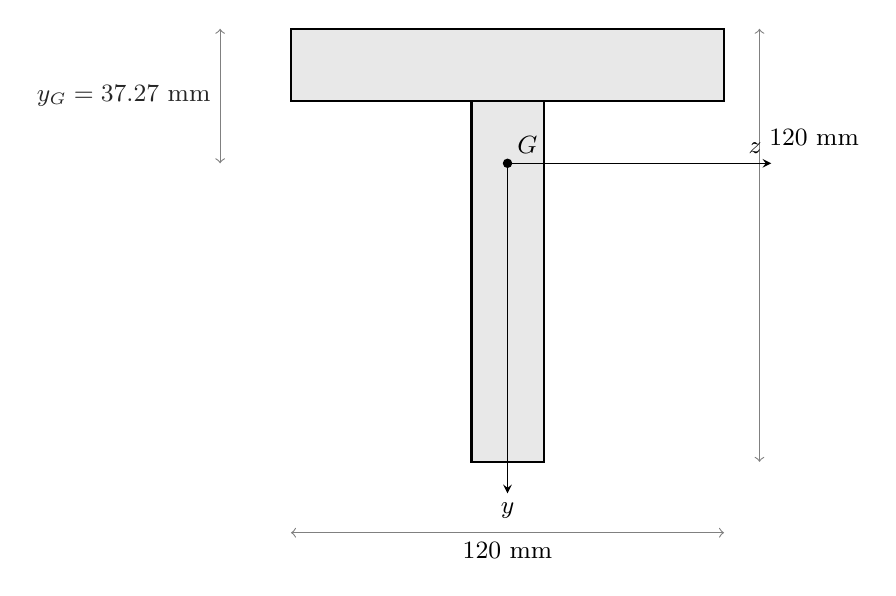
\begin{tikzpicture}
% studium:polygon ala
\filldraw[fill=gray!18,draw=black,thick] (0.0000,0.0000) -- (5.5000,0.0000) -- (5.5000,-0.9167) -- (0.0000,-0.9167) -- cycle;
% studium:polygon alma
\filldraw[fill=gray!18,draw=black,thick] (2.2917,-0.9167) -- (3.2083,-0.9167) -- (3.2083,-5.5000) -- (2.2917,-5.5000) -- cycle;
\draw[<->,gray] (0.0000,-6.4000) -- (5.5000,-6.4000);
\node[font=\small,anchor=north] at (2.7500,-6.4000) {$120$~\mbox{mm}};
\draw[<->,gray] (5.9500,0.0000) -- (5.9500,-5.5000);
\node[font=\small,anchor=west] at (5.9500,-1.3750) {$120$~\mbox{mm}};
% studium:point G z=60 y=410/11
\fill[black] (2.7500,-1.7083) circle (0.06);
\node[font=\small,anchor=south west] at (2.7500,-1.7083) {$G$};
\draw[-stealth,thin] (2.7500,-1.7083) -- (6.1000,-1.7083) node[above left,font=\small] {$z$};
\draw[-stealth,thin] (2.7500,-1.7083) -- (2.7500,-5.9000) node[below,font=\small] {$y$};
\draw[<->,gray] (-0.9000,0.0000) -- (-0.9000,-1.7083);
\node[font=\small,anchor=east,gray!30!black] at (-0.9000,-0.8542) {$y_G = 37.27$~\mbox{mm}};
\end{tikzpicture}}%
\count0=\ht0
\advance\count0 by \dp0
\count2=\wd0
\count4=\dimexpr\textheight/100*38\relax
\count6=\linewidth
\ifnum\count0<1
\count0=1
\fi
\ifnum\count2<1
\count2=1
\fi
\divide\count0 by 4096
\divide\count2 by 4096
\divide\count4 by 4096
\divide\count6 by 4096
\ifnum\count0<1
\count0=1
\fi
\ifnum\count2<1
\count2=1
\fi
\ifnum\count4<1
\count4=1
\fi
\ifnum\count6<1
\count6=1
\fi
\count8=\count2
\ifnum\count0>\count4
\count8=\numexpr\count2*\count4/\count0\relax
\fi
\ifnum\count8>\count6
\resizebox{\linewidth}{!}{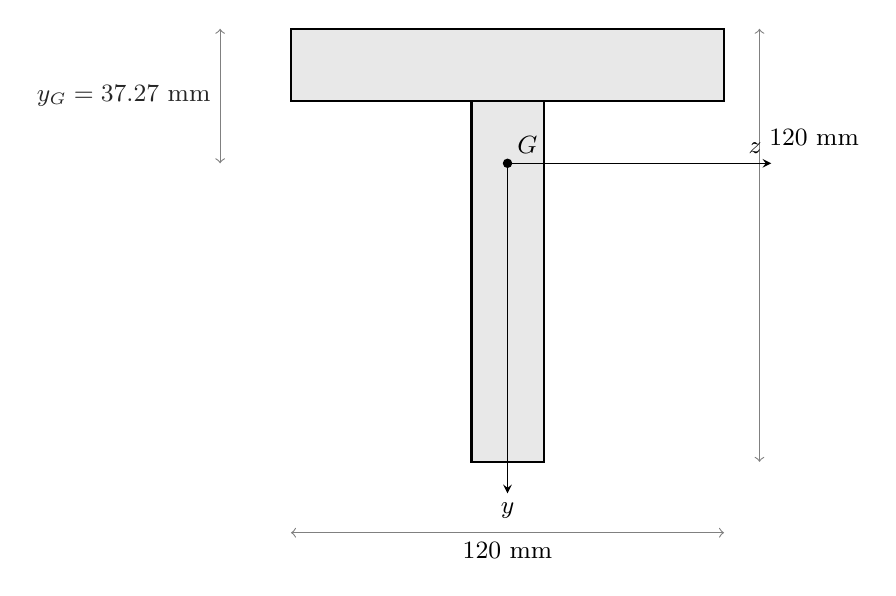
\begin{tikzpicture}
% studium:polygon ala
\filldraw[fill=gray!18,draw=black,thick] (0.0000,0.0000) -- (5.5000,0.0000) -- (5.5000,-0.9167) -- (0.0000,-0.9167) -- cycle;
% studium:polygon alma
\filldraw[fill=gray!18,draw=black,thick] (2.2917,-0.9167) -- (3.2083,-0.9167) -- (3.2083,-5.5000) -- (2.2917,-5.5000) -- cycle;
\draw[<->,gray] (0.0000,-6.4000) -- (5.5000,-6.4000);
\node[font=\small,anchor=north] at (2.7500,-6.4000) {$120$~\mbox{mm}};
\draw[<->,gray] (5.9500,0.0000) -- (5.9500,-5.5000);
\node[font=\small,anchor=west] at (5.9500,-1.3750) {$120$~\mbox{mm}};
% studium:point G z=60 y=410/11
\fill[black] (2.7500,-1.7083) circle (0.06);
\node[font=\small,anchor=south west] at (2.7500,-1.7083) {$G$};
\draw[-stealth,thin] (2.7500,-1.7083) -- (6.1000,-1.7083) node[above left,font=\small] {$z$};
\draw[-stealth,thin] (2.7500,-1.7083) -- (2.7500,-5.9000) node[below,font=\small] {$y$};
\draw[<->,gray] (-0.9000,0.0000) -- (-0.9000,-1.7083);
\node[font=\small,anchor=east,gray!30!black] at (-0.9000,-0.8542) {$y_G = 37.27$~\mbox{mm}};
\end{tikzpicture}}%
\else
\ifnum\count0>\count4
\resizebox{!}{\dimexpr\textheight/100*38\relax}{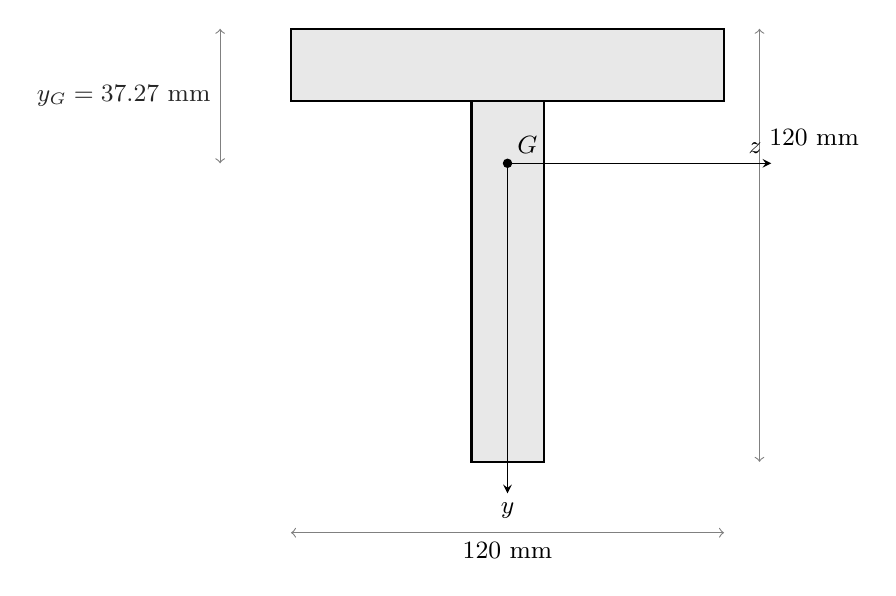
\begin{tikzpicture}
% studium:polygon ala
\filldraw[fill=gray!18,draw=black,thick] (0.0000,0.0000) -- (5.5000,0.0000) -- (5.5000,-0.9167) -- (0.0000,-0.9167) -- cycle;
% studium:polygon alma
\filldraw[fill=gray!18,draw=black,thick] (2.2917,-0.9167) -- (3.2083,-0.9167) -- (3.2083,-5.5000) -- (2.2917,-5.5000) -- cycle;
\draw[<->,gray] (0.0000,-6.4000) -- (5.5000,-6.4000);
\node[font=\small,anchor=north] at (2.7500,-6.4000) {$120$~\mbox{mm}};
\draw[<->,gray] (5.9500,0.0000) -- (5.9500,-5.5000);
\node[font=\small,anchor=west] at (5.9500,-1.3750) {$120$~\mbox{mm}};
% studium:point G z=60 y=410/11
\fill[black] (2.7500,-1.7083) circle (0.06);
\node[font=\small,anchor=south west] at (2.7500,-1.7083) {$G$};
\draw[-stealth,thin] (2.7500,-1.7083) -- (6.1000,-1.7083) node[above left,font=\small] {$z$};
\draw[-stealth,thin] (2.7500,-1.7083) -- (2.7500,-5.9000) node[below,font=\small] {$y$};
\draw[<->,gray] (-0.9000,0.0000) -- (-0.9000,-1.7083);
\node[font=\small,anchor=east,gray!30!black] at (-0.9000,-0.8542) {$y_G = 37.27$~\mbox{mm}};
\end{tikzpicture}}%
\else
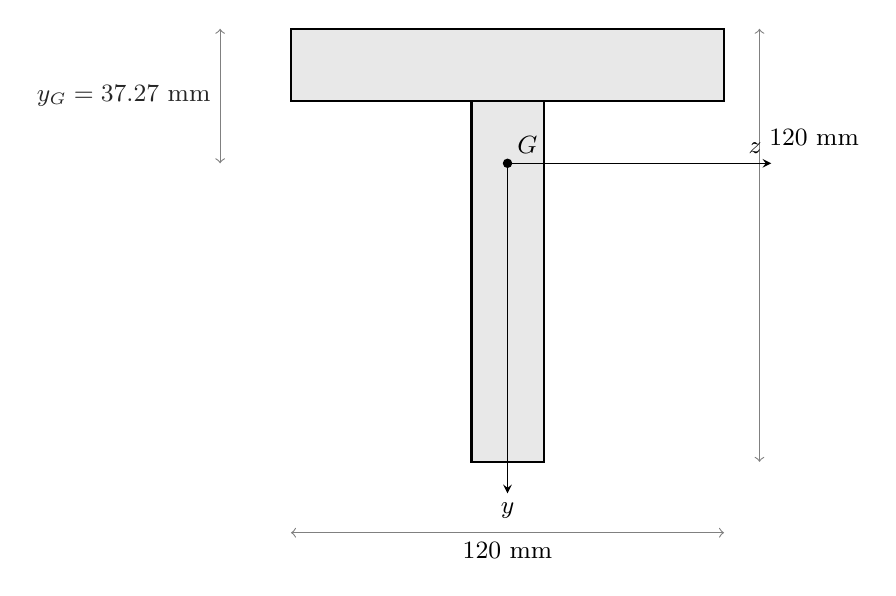
\begin{tikzpicture}
% studium:polygon ala
\filldraw[fill=gray!18,draw=black,thick] (0.0000,0.0000) -- (5.5000,0.0000) -- (5.5000,-0.9167) -- (0.0000,-0.9167) -- cycle;
% studium:polygon alma
\filldraw[fill=gray!18,draw=black,thick] (2.2917,-0.9167) -- (3.2083,-0.9167) -- (3.2083,-5.5000) -- (2.2917,-5.5000) -- cycle;
\draw[<->,gray] (0.0000,-6.4000) -- (5.5000,-6.4000);
\node[font=\small,anchor=north] at (2.7500,-6.4000) {$120$~\mbox{mm}};
\draw[<->,gray] (5.9500,0.0000) -- (5.9500,-5.5000);
\node[font=\small,anchor=west] at (5.9500,-1.3750) {$120$~\mbox{mm}};
% studium:point G z=60 y=410/11
\fill[black] (2.7500,-1.7083) circle (0.06);
\node[font=\small,anchor=south west] at (2.7500,-1.7083) {$G$};
\draw[-stealth,thin] (2.7500,-1.7083) -- (6.1000,-1.7083) node[above left,font=\small] {$z$};
\draw[-stealth,thin] (2.7500,-1.7083) -- (2.7500,-5.9000) node[below,font=\small] {$y$};
\draw[<->,gray] (-0.9000,0.0000) -- (-0.9000,-1.7083);
\node[font=\small,anchor=east,gray!30!black] at (-0.9000,-0.8542) {$y_G = 37.27$~\mbox{mm}};
\end{tikzpicture}%
\fi
\fi
\endgroup
\par\nopagebreak
\studiumcaption{fig:e2-c03-seccion-t}{Sección en T del problema: centro de gravedad \(G\) en el alma, a \(37.27\) mm de la cara superior, y ejes centrales \(y\), \(z\).}
\end{minipage}\par\medskip

\textbf{Resultado e interpretación.}\[\fitmath{y_G \approx 37.3\ \mathrm{mm},\qquad I_z \approx 5.67\times 10^{6}\ \mathrm{mm}^{4}}\]

El centro de gravedad queda a unos $37.3$ mm de la cara superior, es decir, $17.3$ mm por debajo de la cara inferior del ala: está en el alma, no en el ala. Es razonable, porque el alma pesa casi tanto como el ala y tira del centro de gravedad hacia abajo. Los términos de Steiner suman más que los momentos propios.

\par\textbf{Comprobación.} Recalcula los pasos con unidades coherentes y aplica el control específico indicado en la orientación del capítulo.

\textbf{Límites.}\begin{itemize}\item no se incluyen redondeos entre ala y alma\end{itemize}

\textbf{Errores frecuentes.}\begin{itemize}\item medir las distancias desde la cara superior en lugar de hacerlo desde el centro de gravedad de la sección completa
\item olvidar el término $A d^2$
\item afirmar en qué parte de la sección cae el centro de gravedad sin comparar su ordenada con las cotas de cada parte\end{itemize}

\end{studiumworked}

\Needspace{.3\textheight}

\begin{studiumworked}{PRB-0182}

\section{PRB-0182 · Momento flector máximo}

\textbf{Enunciado.} Una viga biapoyada de 6 m de luz soporta una carga uniforme de 12 kN/m en toda su longitud y una carga puntual de 18 kN a 2 m del apoyo izquierdo $A$. Calcule las reacciones y el momento flector máximo, e indique dónde se produce.

\par\medskip\noindent\begin{tabular}{@{}p{.18\linewidth}p{.26\linewidth}p{.48\linewidth}@{}}
\toprule Símbolo & Valor y unidad & Significado\\\midrule
$L$ & $6\,\mathrm{m}$ & luz\\
$q$ & $12\,\mathrm{kN/m}$ & carga uniforme\\
$P$ & $18\,\mathrm{kN}$ & carga puntual\\
$a$ & $2\,\mathrm{m}$ & posición de la carga puntual\\
\bottomrule\end{tabular}\par\medskip

\par\medskip\noindent\begin{minipage}{\linewidth}
\centering
\begingroup
\setbox0=\hbox{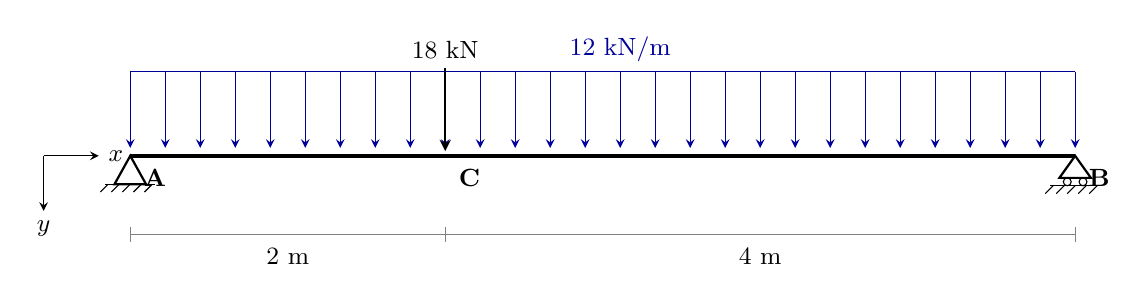
\begin{tikzpicture}
\draw[-stealth,blue!60!black] (0.0000,1.0700) -- (0.0000,0.1000);
\draw[-stealth,blue!60!black] (0.4444,1.0700) -- (0.4444,0.1000);
\draw[-stealth,blue!60!black] (0.8889,1.0700) -- (0.8889,0.1000);
\draw[-stealth,blue!60!black] (1.3333,1.0700) -- (1.3333,0.1000);
\draw[-stealth,blue!60!black] (1.7778,1.0700) -- (1.7778,0.1000);
\draw[-stealth,blue!60!black] (2.2222,1.0700) -- (2.2222,0.1000);
\draw[-stealth,blue!60!black] (2.6667,1.0700) -- (2.6667,0.1000);
\draw[-stealth,blue!60!black] (3.1111,1.0700) -- (3.1111,0.1000);
\draw[-stealth,blue!60!black] (3.5556,1.0700) -- (3.5556,0.1000);
\draw[-stealth,blue!60!black] (4.0000,1.0700) -- (4.0000,0.1000);
\draw[-stealth,blue!60!black] (4.4444,1.0700) -- (4.4444,0.1000);
\draw[-stealth,blue!60!black] (4.8889,1.0700) -- (4.8889,0.1000);
\draw[-stealth,blue!60!black] (5.3333,1.0700) -- (5.3333,0.1000);
\draw[-stealth,blue!60!black] (5.7778,1.0700) -- (5.7778,0.1000);
\draw[-stealth,blue!60!black] (6.2222,1.0700) -- (6.2222,0.1000);
\draw[-stealth,blue!60!black] (6.6667,1.0700) -- (6.6667,0.1000);
\draw[-stealth,blue!60!black] (7.1111,1.0700) -- (7.1111,0.1000);
\draw[-stealth,blue!60!black] (7.5556,1.0700) -- (7.5556,0.1000);
\draw[-stealth,blue!60!black] (8.0000,1.0700) -- (8.0000,0.1000);
\draw[-stealth,blue!60!black] (8.4444,1.0700) -- (8.4444,0.1000);
\draw[-stealth,blue!60!black] (8.8889,1.0700) -- (8.8889,0.1000);
\draw[-stealth,blue!60!black] (9.3333,1.0700) -- (9.3333,0.1000);
\draw[-stealth,blue!60!black] (9.7778,1.0700) -- (9.7778,0.1000);
\draw[-stealth,blue!60!black] (10.2222,1.0700) -- (10.2222,0.1000);
\draw[-stealth,blue!60!black] (10.6667,1.0700) -- (10.6667,0.1000);
\draw[-stealth,blue!60!black] (11.1111,1.0700) -- (11.1111,0.1000);
\draw[-stealth,blue!60!black] (11.5556,1.0700) -- (11.5556,0.1000);
\draw[-stealth,blue!60!black] (12.0000,1.0700) -- (12.0000,0.1000);
% studium:at distributed 0 x=0 to=6 check=span
\draw[blue!60!black] (0.0000,1.0700) -- (0.4444,1.0700) -- (0.8889,1.0700) -- (1.3333,1.0700) -- (1.7778,1.0700) -- (2.2222,1.0700) -- (2.6667,1.0700) -- (3.1111,1.0700) -- (3.5556,1.0700) -- (4.0000,1.0700) -- (4.4444,1.0700) -- (4.8889,1.0700) -- (5.3333,1.0700) -- (5.7778,1.0700) -- (6.2222,1.0700) -- (6.6667,1.0700) -- (7.1111,1.0700) -- (7.5556,1.0700) -- (8.0000,1.0700) -- (8.4444,1.0700) -- (8.8889,1.0700) -- (9.3333,1.0700) -- (9.7778,1.0700) -- (10.2222,1.0700) -- (10.6667,1.0700) -- (11.1111,1.0700) -- (11.5556,1.0700) -- (12.0000,1.0700);
\node[font=\small,anchor=south,blue!60!black] at (6.2222,1.0700) {$12$~\mbox{kN/m}};
\draw[line width=1.6pt] (0,0.0000) -- (12.0000,0.0000);
% studium:at support A x=0 check=first
\draw[thick,fill=white] (0.0000,0.0000) -- (-0.2000,-0.3600) -- (0.2000,-0.3600) -- cycle;
\draw (-0.3200,-0.3600) -- (0.3200,-0.3600);
\draw (-0.2800,-0.3600) -- (-0.3800,-0.4600);
\draw (-0.1400,-0.3600) -- (-0.2400,-0.4600);
\draw (0.0000,-0.3600) -- (-0.1000,-0.4600);
\draw (0.1400,-0.3600) -- (0.0400,-0.4600);
\draw (0.2800,-0.3600) -- (0.1800,-0.4600);
% studium:at support B x=6 check=first
\draw[thick,fill=white] (12.0000,0.0000) -- (11.8000,-0.2800) -- (12.2000,-0.2800) -- cycle;
\draw (11.9000,-0.3300) circle (0.05);
\draw (12.1000,-0.3300) circle (0.05);
\draw (11.6800,-0.3800) -- (12.3200,-0.3800);
\draw (11.7200,-0.3800) -- (11.6200,-0.4800);
\draw (11.8600,-0.3800) -- (11.7600,-0.4800);
\draw (12.0000,-0.3800) -- (11.9000,-0.4800);
\draw (12.1400,-0.3800) -- (12.0400,-0.4800);
\draw (12.2800,-0.3800) -- (12.1800,-0.4800);
% studium:at force 0 x=2 check=tip
\draw[-stealth,thick,black] (4.0000,1.1100) -- (4.0000,0.0600);
\node[font=\small,anchor=south] at (4.0000,1.1100) {$18$~\mbox{kN}};
\node[font=\small\bfseries,anchor=north west] at (0.0500,-0.0500) {A};
\node[font=\small\bfseries,anchor=north west] at (4.0500,-0.0500) {C};
\node[font=\small\bfseries,anchor=north west] at (12.0500,-0.0500) {B};
\draw[gray] (0,-1.0000) -- (12.0000,-1.0000);
\draw[gray] (0.0000,-1.1000) -- (0.0000,-0.9000);
\draw[gray] (4.0000,-1.1000) -- (4.0000,-0.9000);
\draw[gray] (12.0000,-1.1000) -- (12.0000,-0.9000);
\node[font=\small,anchor=north] at (2.0000,-1.0500) {$2$~\mbox{m}};
\node[font=\small,anchor=north] at (8.0000,-1.0500) {$4$~\mbox{m}};
\draw[-stealth] (-1.1,0.0000) -- (-0.4,0.0000) node[right,font=\small] {$x$};
\draw[-stealth] (-1.1,0.0000) -- (-1.1,-0.7000) node[below,font=\small] {$y$};
\end{tikzpicture}}%
\count0=\ht0
\advance\count0 by \dp0
\count2=\wd0
\count4=\dimexpr\textheight/100*38\relax
\count6=\linewidth
\ifnum\count0<1
\count0=1
\fi
\ifnum\count2<1
\count2=1
\fi
\divide\count0 by 4096
\divide\count2 by 4096
\divide\count4 by 4096
\divide\count6 by 4096
\ifnum\count0<1
\count0=1
\fi
\ifnum\count2<1
\count2=1
\fi
\ifnum\count4<1
\count4=1
\fi
\ifnum\count6<1
\count6=1
\fi
\count8=\count2
\ifnum\count0>\count4
\count8=\numexpr\count2*\count4/\count0\relax
\fi
\ifnum\count8>\count6
\resizebox{\linewidth}{!}{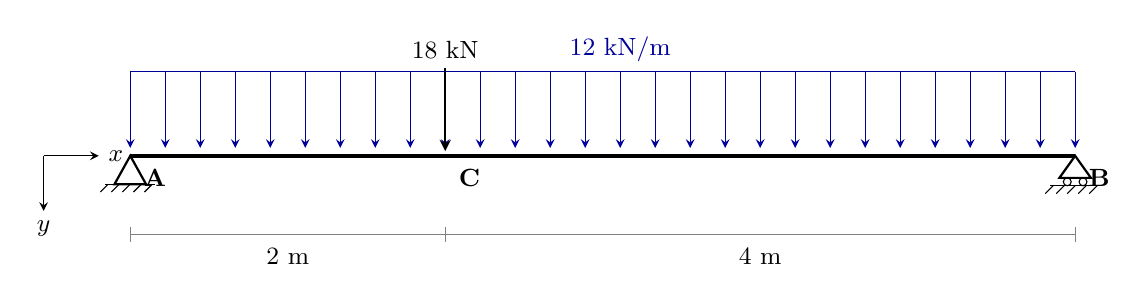
\begin{tikzpicture}
\draw[-stealth,blue!60!black] (0.0000,1.0700) -- (0.0000,0.1000);
\draw[-stealth,blue!60!black] (0.4444,1.0700) -- (0.4444,0.1000);
\draw[-stealth,blue!60!black] (0.8889,1.0700) -- (0.8889,0.1000);
\draw[-stealth,blue!60!black] (1.3333,1.0700) -- (1.3333,0.1000);
\draw[-stealth,blue!60!black] (1.7778,1.0700) -- (1.7778,0.1000);
\draw[-stealth,blue!60!black] (2.2222,1.0700) -- (2.2222,0.1000);
\draw[-stealth,blue!60!black] (2.6667,1.0700) -- (2.6667,0.1000);
\draw[-stealth,blue!60!black] (3.1111,1.0700) -- (3.1111,0.1000);
\draw[-stealth,blue!60!black] (3.5556,1.0700) -- (3.5556,0.1000);
\draw[-stealth,blue!60!black] (4.0000,1.0700) -- (4.0000,0.1000);
\draw[-stealth,blue!60!black] (4.4444,1.0700) -- (4.4444,0.1000);
\draw[-stealth,blue!60!black] (4.8889,1.0700) -- (4.8889,0.1000);
\draw[-stealth,blue!60!black] (5.3333,1.0700) -- (5.3333,0.1000);
\draw[-stealth,blue!60!black] (5.7778,1.0700) -- (5.7778,0.1000);
\draw[-stealth,blue!60!black] (6.2222,1.0700) -- (6.2222,0.1000);
\draw[-stealth,blue!60!black] (6.6667,1.0700) -- (6.6667,0.1000);
\draw[-stealth,blue!60!black] (7.1111,1.0700) -- (7.1111,0.1000);
\draw[-stealth,blue!60!black] (7.5556,1.0700) -- (7.5556,0.1000);
\draw[-stealth,blue!60!black] (8.0000,1.0700) -- (8.0000,0.1000);
\draw[-stealth,blue!60!black] (8.4444,1.0700) -- (8.4444,0.1000);
\draw[-stealth,blue!60!black] (8.8889,1.0700) -- (8.8889,0.1000);
\draw[-stealth,blue!60!black] (9.3333,1.0700) -- (9.3333,0.1000);
\draw[-stealth,blue!60!black] (9.7778,1.0700) -- (9.7778,0.1000);
\draw[-stealth,blue!60!black] (10.2222,1.0700) -- (10.2222,0.1000);
\draw[-stealth,blue!60!black] (10.6667,1.0700) -- (10.6667,0.1000);
\draw[-stealth,blue!60!black] (11.1111,1.0700) -- (11.1111,0.1000);
\draw[-stealth,blue!60!black] (11.5556,1.0700) -- (11.5556,0.1000);
\draw[-stealth,blue!60!black] (12.0000,1.0700) -- (12.0000,0.1000);
% studium:at distributed 0 x=0 to=6 check=span
\draw[blue!60!black] (0.0000,1.0700) -- (0.4444,1.0700) -- (0.8889,1.0700) -- (1.3333,1.0700) -- (1.7778,1.0700) -- (2.2222,1.0700) -- (2.6667,1.0700) -- (3.1111,1.0700) -- (3.5556,1.0700) -- (4.0000,1.0700) -- (4.4444,1.0700) -- (4.8889,1.0700) -- (5.3333,1.0700) -- (5.7778,1.0700) -- (6.2222,1.0700) -- (6.6667,1.0700) -- (7.1111,1.0700) -- (7.5556,1.0700) -- (8.0000,1.0700) -- (8.4444,1.0700) -- (8.8889,1.0700) -- (9.3333,1.0700) -- (9.7778,1.0700) -- (10.2222,1.0700) -- (10.6667,1.0700) -- (11.1111,1.0700) -- (11.5556,1.0700) -- (12.0000,1.0700);
\node[font=\small,anchor=south,blue!60!black] at (6.2222,1.0700) {$12$~\mbox{kN/m}};
\draw[line width=1.6pt] (0,0.0000) -- (12.0000,0.0000);
% studium:at support A x=0 check=first
\draw[thick,fill=white] (0.0000,0.0000) -- (-0.2000,-0.3600) -- (0.2000,-0.3600) -- cycle;
\draw (-0.3200,-0.3600) -- (0.3200,-0.3600);
\draw (-0.2800,-0.3600) -- (-0.3800,-0.4600);
\draw (-0.1400,-0.3600) -- (-0.2400,-0.4600);
\draw (0.0000,-0.3600) -- (-0.1000,-0.4600);
\draw (0.1400,-0.3600) -- (0.0400,-0.4600);
\draw (0.2800,-0.3600) -- (0.1800,-0.4600);
% studium:at support B x=6 check=first
\draw[thick,fill=white] (12.0000,0.0000) -- (11.8000,-0.2800) -- (12.2000,-0.2800) -- cycle;
\draw (11.9000,-0.3300) circle (0.05);
\draw (12.1000,-0.3300) circle (0.05);
\draw (11.6800,-0.3800) -- (12.3200,-0.3800);
\draw (11.7200,-0.3800) -- (11.6200,-0.4800);
\draw (11.8600,-0.3800) -- (11.7600,-0.4800);
\draw (12.0000,-0.3800) -- (11.9000,-0.4800);
\draw (12.1400,-0.3800) -- (12.0400,-0.4800);
\draw (12.2800,-0.3800) -- (12.1800,-0.4800);
% studium:at force 0 x=2 check=tip
\draw[-stealth,thick,black] (4.0000,1.1100) -- (4.0000,0.0600);
\node[font=\small,anchor=south] at (4.0000,1.1100) {$18$~\mbox{kN}};
\node[font=\small\bfseries,anchor=north west] at (0.0500,-0.0500) {A};
\node[font=\small\bfseries,anchor=north west] at (4.0500,-0.0500) {C};
\node[font=\small\bfseries,anchor=north west] at (12.0500,-0.0500) {B};
\draw[gray] (0,-1.0000) -- (12.0000,-1.0000);
\draw[gray] (0.0000,-1.1000) -- (0.0000,-0.9000);
\draw[gray] (4.0000,-1.1000) -- (4.0000,-0.9000);
\draw[gray] (12.0000,-1.1000) -- (12.0000,-0.9000);
\node[font=\small,anchor=north] at (2.0000,-1.0500) {$2$~\mbox{m}};
\node[font=\small,anchor=north] at (8.0000,-1.0500) {$4$~\mbox{m}};
\draw[-stealth] (-1.1,0.0000) -- (-0.4,0.0000) node[right,font=\small] {$x$};
\draw[-stealth] (-1.1,0.0000) -- (-1.1,-0.7000) node[below,font=\small] {$y$};
\end{tikzpicture}}%
\else
\ifnum\count0>\count4
\resizebox{!}{\dimexpr\textheight/100*38\relax}{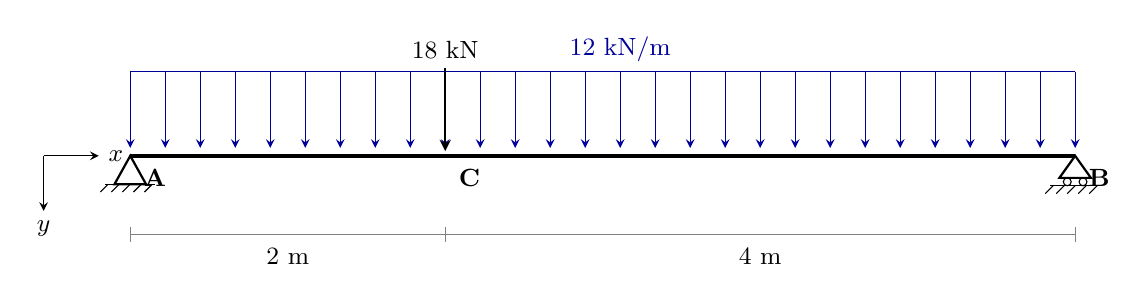
\begin{tikzpicture}
\draw[-stealth,blue!60!black] (0.0000,1.0700) -- (0.0000,0.1000);
\draw[-stealth,blue!60!black] (0.4444,1.0700) -- (0.4444,0.1000);
\draw[-stealth,blue!60!black] (0.8889,1.0700) -- (0.8889,0.1000);
\draw[-stealth,blue!60!black] (1.3333,1.0700) -- (1.3333,0.1000);
\draw[-stealth,blue!60!black] (1.7778,1.0700) -- (1.7778,0.1000);
\draw[-stealth,blue!60!black] (2.2222,1.0700) -- (2.2222,0.1000);
\draw[-stealth,blue!60!black] (2.6667,1.0700) -- (2.6667,0.1000);
\draw[-stealth,blue!60!black] (3.1111,1.0700) -- (3.1111,0.1000);
\draw[-stealth,blue!60!black] (3.5556,1.0700) -- (3.5556,0.1000);
\draw[-stealth,blue!60!black] (4.0000,1.0700) -- (4.0000,0.1000);
\draw[-stealth,blue!60!black] (4.4444,1.0700) -- (4.4444,0.1000);
\draw[-stealth,blue!60!black] (4.8889,1.0700) -- (4.8889,0.1000);
\draw[-stealth,blue!60!black] (5.3333,1.0700) -- (5.3333,0.1000);
\draw[-stealth,blue!60!black] (5.7778,1.0700) -- (5.7778,0.1000);
\draw[-stealth,blue!60!black] (6.2222,1.0700) -- (6.2222,0.1000);
\draw[-stealth,blue!60!black] (6.6667,1.0700) -- (6.6667,0.1000);
\draw[-stealth,blue!60!black] (7.1111,1.0700) -- (7.1111,0.1000);
\draw[-stealth,blue!60!black] (7.5556,1.0700) -- (7.5556,0.1000);
\draw[-stealth,blue!60!black] (8.0000,1.0700) -- (8.0000,0.1000);
\draw[-stealth,blue!60!black] (8.4444,1.0700) -- (8.4444,0.1000);
\draw[-stealth,blue!60!black] (8.8889,1.0700) -- (8.8889,0.1000);
\draw[-stealth,blue!60!black] (9.3333,1.0700) -- (9.3333,0.1000);
\draw[-stealth,blue!60!black] (9.7778,1.0700) -- (9.7778,0.1000);
\draw[-stealth,blue!60!black] (10.2222,1.0700) -- (10.2222,0.1000);
\draw[-stealth,blue!60!black] (10.6667,1.0700) -- (10.6667,0.1000);
\draw[-stealth,blue!60!black] (11.1111,1.0700) -- (11.1111,0.1000);
\draw[-stealth,blue!60!black] (11.5556,1.0700) -- (11.5556,0.1000);
\draw[-stealth,blue!60!black] (12.0000,1.0700) -- (12.0000,0.1000);
% studium:at distributed 0 x=0 to=6 check=span
\draw[blue!60!black] (0.0000,1.0700) -- (0.4444,1.0700) -- (0.8889,1.0700) -- (1.3333,1.0700) -- (1.7778,1.0700) -- (2.2222,1.0700) -- (2.6667,1.0700) -- (3.1111,1.0700) -- (3.5556,1.0700) -- (4.0000,1.0700) -- (4.4444,1.0700) -- (4.8889,1.0700) -- (5.3333,1.0700) -- (5.7778,1.0700) -- (6.2222,1.0700) -- (6.6667,1.0700) -- (7.1111,1.0700) -- (7.5556,1.0700) -- (8.0000,1.0700) -- (8.4444,1.0700) -- (8.8889,1.0700) -- (9.3333,1.0700) -- (9.7778,1.0700) -- (10.2222,1.0700) -- (10.6667,1.0700) -- (11.1111,1.0700) -- (11.5556,1.0700) -- (12.0000,1.0700);
\node[font=\small,anchor=south,blue!60!black] at (6.2222,1.0700) {$12$~\mbox{kN/m}};
\draw[line width=1.6pt] (0,0.0000) -- (12.0000,0.0000);
% studium:at support A x=0 check=first
\draw[thick,fill=white] (0.0000,0.0000) -- (-0.2000,-0.3600) -- (0.2000,-0.3600) -- cycle;
\draw (-0.3200,-0.3600) -- (0.3200,-0.3600);
\draw (-0.2800,-0.3600) -- (-0.3800,-0.4600);
\draw (-0.1400,-0.3600) -- (-0.2400,-0.4600);
\draw (0.0000,-0.3600) -- (-0.1000,-0.4600);
\draw (0.1400,-0.3600) -- (0.0400,-0.4600);
\draw (0.2800,-0.3600) -- (0.1800,-0.4600);
% studium:at support B x=6 check=first
\draw[thick,fill=white] (12.0000,0.0000) -- (11.8000,-0.2800) -- (12.2000,-0.2800) -- cycle;
\draw (11.9000,-0.3300) circle (0.05);
\draw (12.1000,-0.3300) circle (0.05);
\draw (11.6800,-0.3800) -- (12.3200,-0.3800);
\draw (11.7200,-0.3800) -- (11.6200,-0.4800);
\draw (11.8600,-0.3800) -- (11.7600,-0.4800);
\draw (12.0000,-0.3800) -- (11.9000,-0.4800);
\draw (12.1400,-0.3800) -- (12.0400,-0.4800);
\draw (12.2800,-0.3800) -- (12.1800,-0.4800);
% studium:at force 0 x=2 check=tip
\draw[-stealth,thick,black] (4.0000,1.1100) -- (4.0000,0.0600);
\node[font=\small,anchor=south] at (4.0000,1.1100) {$18$~\mbox{kN}};
\node[font=\small\bfseries,anchor=north west] at (0.0500,-0.0500) {A};
\node[font=\small\bfseries,anchor=north west] at (4.0500,-0.0500) {C};
\node[font=\small\bfseries,anchor=north west] at (12.0500,-0.0500) {B};
\draw[gray] (0,-1.0000) -- (12.0000,-1.0000);
\draw[gray] (0.0000,-1.1000) -- (0.0000,-0.9000);
\draw[gray] (4.0000,-1.1000) -- (4.0000,-0.9000);
\draw[gray] (12.0000,-1.1000) -- (12.0000,-0.9000);
\node[font=\small,anchor=north] at (2.0000,-1.0500) {$2$~\mbox{m}};
\node[font=\small,anchor=north] at (8.0000,-1.0500) {$4$~\mbox{m}};
\draw[-stealth] (-1.1,0.0000) -- (-0.4,0.0000) node[right,font=\small] {$x$};
\draw[-stealth] (-1.1,0.0000) -- (-1.1,-0.7000) node[below,font=\small] {$y$};
\end{tikzpicture}}%
\else
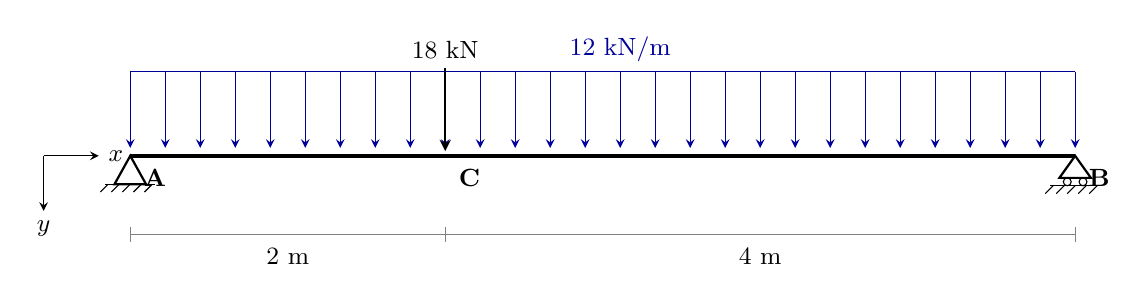
\begin{tikzpicture}
\draw[-stealth,blue!60!black] (0.0000,1.0700) -- (0.0000,0.1000);
\draw[-stealth,blue!60!black] (0.4444,1.0700) -- (0.4444,0.1000);
\draw[-stealth,blue!60!black] (0.8889,1.0700) -- (0.8889,0.1000);
\draw[-stealth,blue!60!black] (1.3333,1.0700) -- (1.3333,0.1000);
\draw[-stealth,blue!60!black] (1.7778,1.0700) -- (1.7778,0.1000);
\draw[-stealth,blue!60!black] (2.2222,1.0700) -- (2.2222,0.1000);
\draw[-stealth,blue!60!black] (2.6667,1.0700) -- (2.6667,0.1000);
\draw[-stealth,blue!60!black] (3.1111,1.0700) -- (3.1111,0.1000);
\draw[-stealth,blue!60!black] (3.5556,1.0700) -- (3.5556,0.1000);
\draw[-stealth,blue!60!black] (4.0000,1.0700) -- (4.0000,0.1000);
\draw[-stealth,blue!60!black] (4.4444,1.0700) -- (4.4444,0.1000);
\draw[-stealth,blue!60!black] (4.8889,1.0700) -- (4.8889,0.1000);
\draw[-stealth,blue!60!black] (5.3333,1.0700) -- (5.3333,0.1000);
\draw[-stealth,blue!60!black] (5.7778,1.0700) -- (5.7778,0.1000);
\draw[-stealth,blue!60!black] (6.2222,1.0700) -- (6.2222,0.1000);
\draw[-stealth,blue!60!black] (6.6667,1.0700) -- (6.6667,0.1000);
\draw[-stealth,blue!60!black] (7.1111,1.0700) -- (7.1111,0.1000);
\draw[-stealth,blue!60!black] (7.5556,1.0700) -- (7.5556,0.1000);
\draw[-stealth,blue!60!black] (8.0000,1.0700) -- (8.0000,0.1000);
\draw[-stealth,blue!60!black] (8.4444,1.0700) -- (8.4444,0.1000);
\draw[-stealth,blue!60!black] (8.8889,1.0700) -- (8.8889,0.1000);
\draw[-stealth,blue!60!black] (9.3333,1.0700) -- (9.3333,0.1000);
\draw[-stealth,blue!60!black] (9.7778,1.0700) -- (9.7778,0.1000);
\draw[-stealth,blue!60!black] (10.2222,1.0700) -- (10.2222,0.1000);
\draw[-stealth,blue!60!black] (10.6667,1.0700) -- (10.6667,0.1000);
\draw[-stealth,blue!60!black] (11.1111,1.0700) -- (11.1111,0.1000);
\draw[-stealth,blue!60!black] (11.5556,1.0700) -- (11.5556,0.1000);
\draw[-stealth,blue!60!black] (12.0000,1.0700) -- (12.0000,0.1000);
% studium:at distributed 0 x=0 to=6 check=span
\draw[blue!60!black] (0.0000,1.0700) -- (0.4444,1.0700) -- (0.8889,1.0700) -- (1.3333,1.0700) -- (1.7778,1.0700) -- (2.2222,1.0700) -- (2.6667,1.0700) -- (3.1111,1.0700) -- (3.5556,1.0700) -- (4.0000,1.0700) -- (4.4444,1.0700) -- (4.8889,1.0700) -- (5.3333,1.0700) -- (5.7778,1.0700) -- (6.2222,1.0700) -- (6.6667,1.0700) -- (7.1111,1.0700) -- (7.5556,1.0700) -- (8.0000,1.0700) -- (8.4444,1.0700) -- (8.8889,1.0700) -- (9.3333,1.0700) -- (9.7778,1.0700) -- (10.2222,1.0700) -- (10.6667,1.0700) -- (11.1111,1.0700) -- (11.5556,1.0700) -- (12.0000,1.0700);
\node[font=\small,anchor=south,blue!60!black] at (6.2222,1.0700) {$12$~\mbox{kN/m}};
\draw[line width=1.6pt] (0,0.0000) -- (12.0000,0.0000);
% studium:at support A x=0 check=first
\draw[thick,fill=white] (0.0000,0.0000) -- (-0.2000,-0.3600) -- (0.2000,-0.3600) -- cycle;
\draw (-0.3200,-0.3600) -- (0.3200,-0.3600);
\draw (-0.2800,-0.3600) -- (-0.3800,-0.4600);
\draw (-0.1400,-0.3600) -- (-0.2400,-0.4600);
\draw (0.0000,-0.3600) -- (-0.1000,-0.4600);
\draw (0.1400,-0.3600) -- (0.0400,-0.4600);
\draw (0.2800,-0.3600) -- (0.1800,-0.4600);
% studium:at support B x=6 check=first
\draw[thick,fill=white] (12.0000,0.0000) -- (11.8000,-0.2800) -- (12.2000,-0.2800) -- cycle;
\draw (11.9000,-0.3300) circle (0.05);
\draw (12.1000,-0.3300) circle (0.05);
\draw (11.6800,-0.3800) -- (12.3200,-0.3800);
\draw (11.7200,-0.3800) -- (11.6200,-0.4800);
\draw (11.8600,-0.3800) -- (11.7600,-0.4800);
\draw (12.0000,-0.3800) -- (11.9000,-0.4800);
\draw (12.1400,-0.3800) -- (12.0400,-0.4800);
\draw (12.2800,-0.3800) -- (12.1800,-0.4800);
% studium:at force 0 x=2 check=tip
\draw[-stealth,thick,black] (4.0000,1.1100) -- (4.0000,0.0600);
\node[font=\small,anchor=south] at (4.0000,1.1100) {$18$~\mbox{kN}};
\node[font=\small\bfseries,anchor=north west] at (0.0500,-0.0500) {A};
\node[font=\small\bfseries,anchor=north west] at (4.0500,-0.0500) {C};
\node[font=\small\bfseries,anchor=north west] at (12.0500,-0.0500) {B};
\draw[gray] (0,-1.0000) -- (12.0000,-1.0000);
\draw[gray] (0.0000,-1.1000) -- (0.0000,-0.9000);
\draw[gray] (4.0000,-1.1000) -- (4.0000,-0.9000);
\draw[gray] (12.0000,-1.1000) -- (12.0000,-0.9000);
\node[font=\small,anchor=north] at (2.0000,-1.0500) {$2$~\mbox{m}};
\node[font=\small,anchor=north] at (8.0000,-1.0500) {$4$~\mbox{m}};
\draw[-stealth] (-1.1,0.0000) -- (-0.4,0.0000) node[right,font=\small] {$x$};
\draw[-stealth] (-1.1,0.0000) -- (-1.1,-0.7000) node[below,font=\small] {$y$};
\end{tikzpicture}%
\fi
\fi
\endgroup
\par\nopagebreak
\studiumcaption{fig:e2-c03-biap-enunciado}{Viga biapoyada con carga uniforme y carga puntual.}
\end{minipage}\par\medskip

\textbf{Hipótesis.}\begin{itemize}\item viga isostática biapoyada
\item cortante positivo si levanta la cara izquierda y flector positivo si comprime arriba\end{itemize}

\textbf{Modelo y desarrollo.}

Flector en el tramo derecho de la carga puntual.\[\fitmath{M_z(x) = R_A\,x - \frac{q\,x^{2}}{2} - P\,(x - a)}\]

\textbf{Procedimiento.}\begin{itemize}\item Momentos respecto a $A$: $R_B L = qL\cdot L/2 + P a$.
\item Equilibrio vertical: $R_A + R_B = qL + P$.
\item En el tramo $x > a$ el cortante es $C_y = R_A - qx - P$ y se anula en $x = 2.5$ m.
\item El flector máximo es el flector en ese punto.\end{itemize}

\textbf{Cálculo de los pasos.}

\begin{enumerate}

\item Reacción en B, de los momentos respecto a A.

\[\fitmath{y_{1}=\frac{12\cdot 6\cdot 3+18\cdot 2}{6}\approx 42\,\mathrm{kN}}\]

\item Reacción en A, del equilibrio vertical.

\[\fitmath{y_{2}=12\cdot 6+18-\frac{12\cdot 6\cdot 3+18\cdot 2}{6}\approx 48\,\mathrm{kN}}\]

\item Abscisa donde se anula el cortante (x mayor que a).

\[\fitmath{y_{3}=\frac{48-18}{12}\approx 2.5\,\mathrm{m}}\]

\item Flector máximo.

\[\fitmath{y_{4}=48\cdot 2.5-\frac{12\cdot {2.5}^{2}}{2}-18\cdot \left(2.5-2\right)\approx 73.5\,\mathrm{kN m}}\]

\end{enumerate}

\par\medskip\noindent\begin{minipage}{\linewidth}
\centering
\begingroup
\setbox0=\hbox{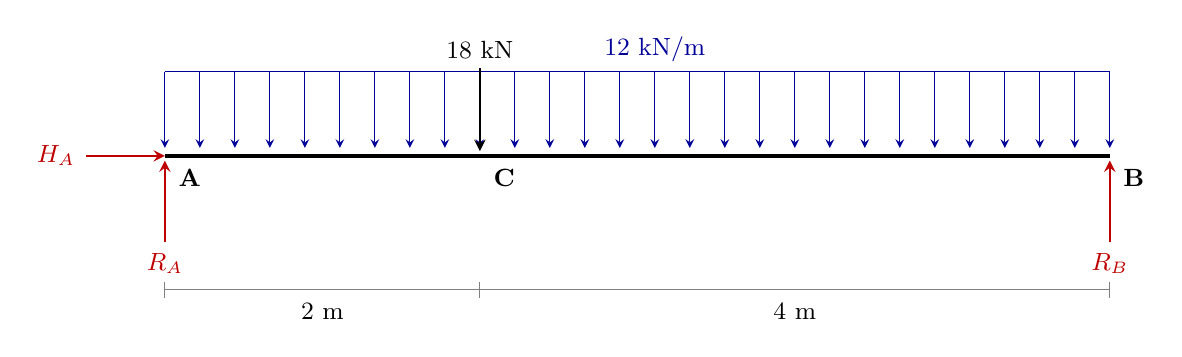
\begin{tikzpicture}
\draw[-stealth,blue!60!black] (0.0000,1.0700) -- (0.0000,0.1000);
\draw[-stealth,blue!60!black] (0.4444,1.0700) -- (0.4444,0.1000);
\draw[-stealth,blue!60!black] (0.8889,1.0700) -- (0.8889,0.1000);
\draw[-stealth,blue!60!black] (1.3333,1.0700) -- (1.3333,0.1000);
\draw[-stealth,blue!60!black] (1.7778,1.0700) -- (1.7778,0.1000);
\draw[-stealth,blue!60!black] (2.2222,1.0700) -- (2.2222,0.1000);
\draw[-stealth,blue!60!black] (2.6667,1.0700) -- (2.6667,0.1000);
\draw[-stealth,blue!60!black] (3.1111,1.0700) -- (3.1111,0.1000);
\draw[-stealth,blue!60!black] (3.5556,1.0700) -- (3.5556,0.1000);
\draw[-stealth,blue!60!black] (4.0000,1.0700) -- (4.0000,0.1000);
\draw[-stealth,blue!60!black] (4.4444,1.0700) -- (4.4444,0.1000);
\draw[-stealth,blue!60!black] (4.8889,1.0700) -- (4.8889,0.1000);
\draw[-stealth,blue!60!black] (5.3333,1.0700) -- (5.3333,0.1000);
\draw[-stealth,blue!60!black] (5.7778,1.0700) -- (5.7778,0.1000);
\draw[-stealth,blue!60!black] (6.2222,1.0700) -- (6.2222,0.1000);
\draw[-stealth,blue!60!black] (6.6667,1.0700) -- (6.6667,0.1000);
\draw[-stealth,blue!60!black] (7.1111,1.0700) -- (7.1111,0.1000);
\draw[-stealth,blue!60!black] (7.5556,1.0700) -- (7.5556,0.1000);
\draw[-stealth,blue!60!black] (8.0000,1.0700) -- (8.0000,0.1000);
\draw[-stealth,blue!60!black] (8.4444,1.0700) -- (8.4444,0.1000);
\draw[-stealth,blue!60!black] (8.8889,1.0700) -- (8.8889,0.1000);
\draw[-stealth,blue!60!black] (9.3333,1.0700) -- (9.3333,0.1000);
\draw[-stealth,blue!60!black] (9.7778,1.0700) -- (9.7778,0.1000);
\draw[-stealth,blue!60!black] (10.2222,1.0700) -- (10.2222,0.1000);
\draw[-stealth,blue!60!black] (10.6667,1.0700) -- (10.6667,0.1000);
\draw[-stealth,blue!60!black] (11.1111,1.0700) -- (11.1111,0.1000);
\draw[-stealth,blue!60!black] (11.5556,1.0700) -- (11.5556,0.1000);
\draw[-stealth,blue!60!black] (12.0000,1.0700) -- (12.0000,0.1000);
% studium:at distributed 0 x=0 to=6 check=span
\draw[blue!60!black] (0.0000,1.0700) -- (0.4444,1.0700) -- (0.8889,1.0700) -- (1.3333,1.0700) -- (1.7778,1.0700) -- (2.2222,1.0700) -- (2.6667,1.0700) -- (3.1111,1.0700) -- (3.5556,1.0700) -- (4.0000,1.0700) -- (4.4444,1.0700) -- (4.8889,1.0700) -- (5.3333,1.0700) -- (5.7778,1.0700) -- (6.2222,1.0700) -- (6.6667,1.0700) -- (7.1111,1.0700) -- (7.5556,1.0700) -- (8.0000,1.0700) -- (8.4444,1.0700) -- (8.8889,1.0700) -- (9.3333,1.0700) -- (9.7778,1.0700) -- (10.2222,1.0700) -- (10.6667,1.0700) -- (11.1111,1.0700) -- (11.5556,1.0700) -- (12.0000,1.0700);
\node[font=\small,anchor=south,blue!60!black] at (6.2222,1.0700) {$12$~\mbox{kN/m}};
\draw[line width=1.6pt] (0,0.0000) -- (12.0000,0.0000);
% studium:at force 0 x=2 check=tip
\draw[-stealth,thick,black] (4.0000,1.1100) -- (4.0000,0.0600);
\node[font=\small,anchor=south] at (4.0000,1.1100) {$18$~\mbox{kN}};
% studium:at reaction H_A x=0 check=tip
\draw[-stealth,thick,red!75!black] (-1.0000,0.0000) -- (0.0000,0.0000);
\node[font=\small,anchor=east,red!75!black] at (-1.0200,0.0000) {$H_{A}$};
% studium:at reaction R_A x=0 check=tip
\draw[-stealth,thick,red!75!black] (0.0000,-1.1000) -- (0.0000,-0.0600);
\node[font=\small,anchor=north,red!75!black] at (0.0000,-1.1200) {$R_{A}$};
% studium:at reaction R_B x=6 check=tip
\draw[-stealth,thick,red!75!black] (12.0000,-1.1000) -- (12.0000,-0.0600);
\node[font=\small,anchor=north,red!75!black] at (12.0000,-1.1200) {$R_{B}$};
\node[font=\small\bfseries,anchor=north west] at (0.0500,-0.0500) {A};
\node[font=\small\bfseries,anchor=north west] at (4.0500,-0.0500) {C};
\node[font=\small\bfseries,anchor=north west] at (12.0500,-0.0500) {B};
\draw[gray] (0,-1.7000) -- (12.0000,-1.7000);
\draw[gray] (0.0000,-1.8000) -- (0.0000,-1.6000);
\draw[gray] (4.0000,-1.8000) -- (4.0000,-1.6000);
\draw[gray] (12.0000,-1.8000) -- (12.0000,-1.6000);
\node[font=\small,anchor=north] at (2.0000,-1.7500) {$2$~\mbox{m}};
\node[font=\small,anchor=north] at (8.0000,-1.7500) {$4$~\mbox{m}};
\end{tikzpicture}}%
\count0=\ht0
\advance\count0 by \dp0
\count2=\wd0
\count4=\dimexpr\textheight/100*38\relax
\count6=\linewidth
\ifnum\count0<1
\count0=1
\fi
\ifnum\count2<1
\count2=1
\fi
\divide\count0 by 4096
\divide\count2 by 4096
\divide\count4 by 4096
\divide\count6 by 4096
\ifnum\count0<1
\count0=1
\fi
\ifnum\count2<1
\count2=1
\fi
\ifnum\count4<1
\count4=1
\fi
\ifnum\count6<1
\count6=1
\fi
\count8=\count2
\ifnum\count0>\count4
\count8=\numexpr\count2*\count4/\count0\relax
\fi
\ifnum\count8>\count6
\resizebox{\linewidth}{!}{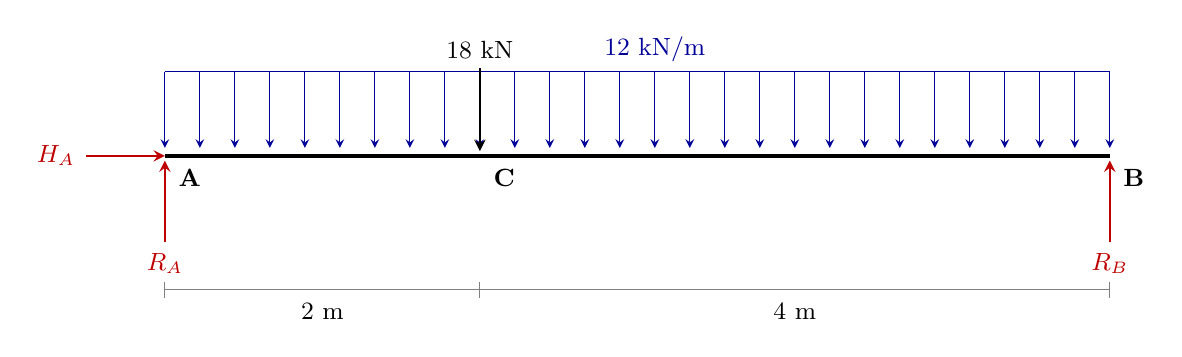
\begin{tikzpicture}
\draw[-stealth,blue!60!black] (0.0000,1.0700) -- (0.0000,0.1000);
\draw[-stealth,blue!60!black] (0.4444,1.0700) -- (0.4444,0.1000);
\draw[-stealth,blue!60!black] (0.8889,1.0700) -- (0.8889,0.1000);
\draw[-stealth,blue!60!black] (1.3333,1.0700) -- (1.3333,0.1000);
\draw[-stealth,blue!60!black] (1.7778,1.0700) -- (1.7778,0.1000);
\draw[-stealth,blue!60!black] (2.2222,1.0700) -- (2.2222,0.1000);
\draw[-stealth,blue!60!black] (2.6667,1.0700) -- (2.6667,0.1000);
\draw[-stealth,blue!60!black] (3.1111,1.0700) -- (3.1111,0.1000);
\draw[-stealth,blue!60!black] (3.5556,1.0700) -- (3.5556,0.1000);
\draw[-stealth,blue!60!black] (4.0000,1.0700) -- (4.0000,0.1000);
\draw[-stealth,blue!60!black] (4.4444,1.0700) -- (4.4444,0.1000);
\draw[-stealth,blue!60!black] (4.8889,1.0700) -- (4.8889,0.1000);
\draw[-stealth,blue!60!black] (5.3333,1.0700) -- (5.3333,0.1000);
\draw[-stealth,blue!60!black] (5.7778,1.0700) -- (5.7778,0.1000);
\draw[-stealth,blue!60!black] (6.2222,1.0700) -- (6.2222,0.1000);
\draw[-stealth,blue!60!black] (6.6667,1.0700) -- (6.6667,0.1000);
\draw[-stealth,blue!60!black] (7.1111,1.0700) -- (7.1111,0.1000);
\draw[-stealth,blue!60!black] (7.5556,1.0700) -- (7.5556,0.1000);
\draw[-stealth,blue!60!black] (8.0000,1.0700) -- (8.0000,0.1000);
\draw[-stealth,blue!60!black] (8.4444,1.0700) -- (8.4444,0.1000);
\draw[-stealth,blue!60!black] (8.8889,1.0700) -- (8.8889,0.1000);
\draw[-stealth,blue!60!black] (9.3333,1.0700) -- (9.3333,0.1000);
\draw[-stealth,blue!60!black] (9.7778,1.0700) -- (9.7778,0.1000);
\draw[-stealth,blue!60!black] (10.2222,1.0700) -- (10.2222,0.1000);
\draw[-stealth,blue!60!black] (10.6667,1.0700) -- (10.6667,0.1000);
\draw[-stealth,blue!60!black] (11.1111,1.0700) -- (11.1111,0.1000);
\draw[-stealth,blue!60!black] (11.5556,1.0700) -- (11.5556,0.1000);
\draw[-stealth,blue!60!black] (12.0000,1.0700) -- (12.0000,0.1000);
% studium:at distributed 0 x=0 to=6 check=span
\draw[blue!60!black] (0.0000,1.0700) -- (0.4444,1.0700) -- (0.8889,1.0700) -- (1.3333,1.0700) -- (1.7778,1.0700) -- (2.2222,1.0700) -- (2.6667,1.0700) -- (3.1111,1.0700) -- (3.5556,1.0700) -- (4.0000,1.0700) -- (4.4444,1.0700) -- (4.8889,1.0700) -- (5.3333,1.0700) -- (5.7778,1.0700) -- (6.2222,1.0700) -- (6.6667,1.0700) -- (7.1111,1.0700) -- (7.5556,1.0700) -- (8.0000,1.0700) -- (8.4444,1.0700) -- (8.8889,1.0700) -- (9.3333,1.0700) -- (9.7778,1.0700) -- (10.2222,1.0700) -- (10.6667,1.0700) -- (11.1111,1.0700) -- (11.5556,1.0700) -- (12.0000,1.0700);
\node[font=\small,anchor=south,blue!60!black] at (6.2222,1.0700) {$12$~\mbox{kN/m}};
\draw[line width=1.6pt] (0,0.0000) -- (12.0000,0.0000);
% studium:at force 0 x=2 check=tip
\draw[-stealth,thick,black] (4.0000,1.1100) -- (4.0000,0.0600);
\node[font=\small,anchor=south] at (4.0000,1.1100) {$18$~\mbox{kN}};
% studium:at reaction H_A x=0 check=tip
\draw[-stealth,thick,red!75!black] (-1.0000,0.0000) -- (0.0000,0.0000);
\node[font=\small,anchor=east,red!75!black] at (-1.0200,0.0000) {$H_{A}$};
% studium:at reaction R_A x=0 check=tip
\draw[-stealth,thick,red!75!black] (0.0000,-1.1000) -- (0.0000,-0.0600);
\node[font=\small,anchor=north,red!75!black] at (0.0000,-1.1200) {$R_{A}$};
% studium:at reaction R_B x=6 check=tip
\draw[-stealth,thick,red!75!black] (12.0000,-1.1000) -- (12.0000,-0.0600);
\node[font=\small,anchor=north,red!75!black] at (12.0000,-1.1200) {$R_{B}$};
\node[font=\small\bfseries,anchor=north west] at (0.0500,-0.0500) {A};
\node[font=\small\bfseries,anchor=north west] at (4.0500,-0.0500) {C};
\node[font=\small\bfseries,anchor=north west] at (12.0500,-0.0500) {B};
\draw[gray] (0,-1.7000) -- (12.0000,-1.7000);
\draw[gray] (0.0000,-1.8000) -- (0.0000,-1.6000);
\draw[gray] (4.0000,-1.8000) -- (4.0000,-1.6000);
\draw[gray] (12.0000,-1.8000) -- (12.0000,-1.6000);
\node[font=\small,anchor=north] at (2.0000,-1.7500) {$2$~\mbox{m}};
\node[font=\small,anchor=north] at (8.0000,-1.7500) {$4$~\mbox{m}};
\end{tikzpicture}}%
\else
\ifnum\count0>\count4
\resizebox{!}{\dimexpr\textheight/100*38\relax}{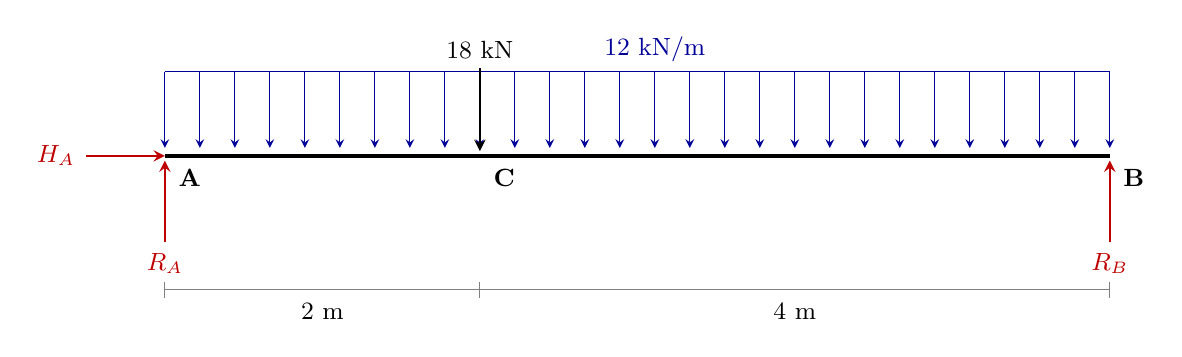
\begin{tikzpicture}
\draw[-stealth,blue!60!black] (0.0000,1.0700) -- (0.0000,0.1000);
\draw[-stealth,blue!60!black] (0.4444,1.0700) -- (0.4444,0.1000);
\draw[-stealth,blue!60!black] (0.8889,1.0700) -- (0.8889,0.1000);
\draw[-stealth,blue!60!black] (1.3333,1.0700) -- (1.3333,0.1000);
\draw[-stealth,blue!60!black] (1.7778,1.0700) -- (1.7778,0.1000);
\draw[-stealth,blue!60!black] (2.2222,1.0700) -- (2.2222,0.1000);
\draw[-stealth,blue!60!black] (2.6667,1.0700) -- (2.6667,0.1000);
\draw[-stealth,blue!60!black] (3.1111,1.0700) -- (3.1111,0.1000);
\draw[-stealth,blue!60!black] (3.5556,1.0700) -- (3.5556,0.1000);
\draw[-stealth,blue!60!black] (4.0000,1.0700) -- (4.0000,0.1000);
\draw[-stealth,blue!60!black] (4.4444,1.0700) -- (4.4444,0.1000);
\draw[-stealth,blue!60!black] (4.8889,1.0700) -- (4.8889,0.1000);
\draw[-stealth,blue!60!black] (5.3333,1.0700) -- (5.3333,0.1000);
\draw[-stealth,blue!60!black] (5.7778,1.0700) -- (5.7778,0.1000);
\draw[-stealth,blue!60!black] (6.2222,1.0700) -- (6.2222,0.1000);
\draw[-stealth,blue!60!black] (6.6667,1.0700) -- (6.6667,0.1000);
\draw[-stealth,blue!60!black] (7.1111,1.0700) -- (7.1111,0.1000);
\draw[-stealth,blue!60!black] (7.5556,1.0700) -- (7.5556,0.1000);
\draw[-stealth,blue!60!black] (8.0000,1.0700) -- (8.0000,0.1000);
\draw[-stealth,blue!60!black] (8.4444,1.0700) -- (8.4444,0.1000);
\draw[-stealth,blue!60!black] (8.8889,1.0700) -- (8.8889,0.1000);
\draw[-stealth,blue!60!black] (9.3333,1.0700) -- (9.3333,0.1000);
\draw[-stealth,blue!60!black] (9.7778,1.0700) -- (9.7778,0.1000);
\draw[-stealth,blue!60!black] (10.2222,1.0700) -- (10.2222,0.1000);
\draw[-stealth,blue!60!black] (10.6667,1.0700) -- (10.6667,0.1000);
\draw[-stealth,blue!60!black] (11.1111,1.0700) -- (11.1111,0.1000);
\draw[-stealth,blue!60!black] (11.5556,1.0700) -- (11.5556,0.1000);
\draw[-stealth,blue!60!black] (12.0000,1.0700) -- (12.0000,0.1000);
% studium:at distributed 0 x=0 to=6 check=span
\draw[blue!60!black] (0.0000,1.0700) -- (0.4444,1.0700) -- (0.8889,1.0700) -- (1.3333,1.0700) -- (1.7778,1.0700) -- (2.2222,1.0700) -- (2.6667,1.0700) -- (3.1111,1.0700) -- (3.5556,1.0700) -- (4.0000,1.0700) -- (4.4444,1.0700) -- (4.8889,1.0700) -- (5.3333,1.0700) -- (5.7778,1.0700) -- (6.2222,1.0700) -- (6.6667,1.0700) -- (7.1111,1.0700) -- (7.5556,1.0700) -- (8.0000,1.0700) -- (8.4444,1.0700) -- (8.8889,1.0700) -- (9.3333,1.0700) -- (9.7778,1.0700) -- (10.2222,1.0700) -- (10.6667,1.0700) -- (11.1111,1.0700) -- (11.5556,1.0700) -- (12.0000,1.0700);
\node[font=\small,anchor=south,blue!60!black] at (6.2222,1.0700) {$12$~\mbox{kN/m}};
\draw[line width=1.6pt] (0,0.0000) -- (12.0000,0.0000);
% studium:at force 0 x=2 check=tip
\draw[-stealth,thick,black] (4.0000,1.1100) -- (4.0000,0.0600);
\node[font=\small,anchor=south] at (4.0000,1.1100) {$18$~\mbox{kN}};
% studium:at reaction H_A x=0 check=tip
\draw[-stealth,thick,red!75!black] (-1.0000,0.0000) -- (0.0000,0.0000);
\node[font=\small,anchor=east,red!75!black] at (-1.0200,0.0000) {$H_{A}$};
% studium:at reaction R_A x=0 check=tip
\draw[-stealth,thick,red!75!black] (0.0000,-1.1000) -- (0.0000,-0.0600);
\node[font=\small,anchor=north,red!75!black] at (0.0000,-1.1200) {$R_{A}$};
% studium:at reaction R_B x=6 check=tip
\draw[-stealth,thick,red!75!black] (12.0000,-1.1000) -- (12.0000,-0.0600);
\node[font=\small,anchor=north,red!75!black] at (12.0000,-1.1200) {$R_{B}$};
\node[font=\small\bfseries,anchor=north west] at (0.0500,-0.0500) {A};
\node[font=\small\bfseries,anchor=north west] at (4.0500,-0.0500) {C};
\node[font=\small\bfseries,anchor=north west] at (12.0500,-0.0500) {B};
\draw[gray] (0,-1.7000) -- (12.0000,-1.7000);
\draw[gray] (0.0000,-1.8000) -- (0.0000,-1.6000);
\draw[gray] (4.0000,-1.8000) -- (4.0000,-1.6000);
\draw[gray] (12.0000,-1.8000) -- (12.0000,-1.6000);
\node[font=\small,anchor=north] at (2.0000,-1.7500) {$2$~\mbox{m}};
\node[font=\small,anchor=north] at (8.0000,-1.7500) {$4$~\mbox{m}};
\end{tikzpicture}}%
\else
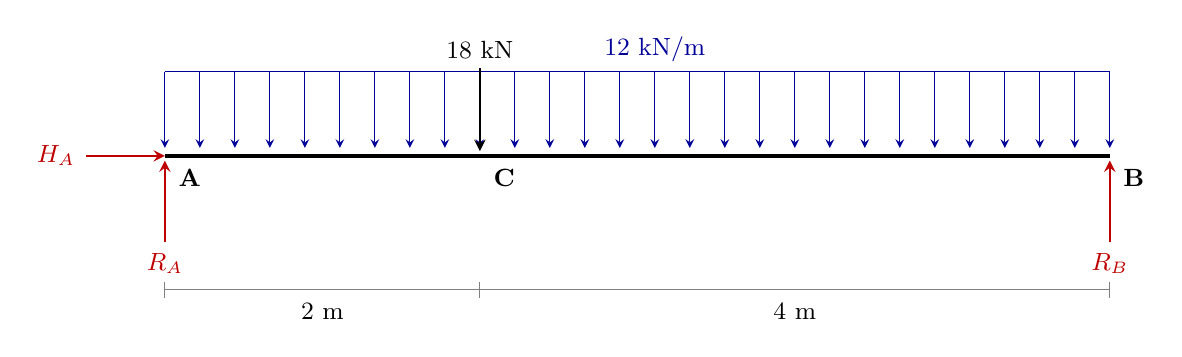
\begin{tikzpicture}
\draw[-stealth,blue!60!black] (0.0000,1.0700) -- (0.0000,0.1000);
\draw[-stealth,blue!60!black] (0.4444,1.0700) -- (0.4444,0.1000);
\draw[-stealth,blue!60!black] (0.8889,1.0700) -- (0.8889,0.1000);
\draw[-stealth,blue!60!black] (1.3333,1.0700) -- (1.3333,0.1000);
\draw[-stealth,blue!60!black] (1.7778,1.0700) -- (1.7778,0.1000);
\draw[-stealth,blue!60!black] (2.2222,1.0700) -- (2.2222,0.1000);
\draw[-stealth,blue!60!black] (2.6667,1.0700) -- (2.6667,0.1000);
\draw[-stealth,blue!60!black] (3.1111,1.0700) -- (3.1111,0.1000);
\draw[-stealth,blue!60!black] (3.5556,1.0700) -- (3.5556,0.1000);
\draw[-stealth,blue!60!black] (4.0000,1.0700) -- (4.0000,0.1000);
\draw[-stealth,blue!60!black] (4.4444,1.0700) -- (4.4444,0.1000);
\draw[-stealth,blue!60!black] (4.8889,1.0700) -- (4.8889,0.1000);
\draw[-stealth,blue!60!black] (5.3333,1.0700) -- (5.3333,0.1000);
\draw[-stealth,blue!60!black] (5.7778,1.0700) -- (5.7778,0.1000);
\draw[-stealth,blue!60!black] (6.2222,1.0700) -- (6.2222,0.1000);
\draw[-stealth,blue!60!black] (6.6667,1.0700) -- (6.6667,0.1000);
\draw[-stealth,blue!60!black] (7.1111,1.0700) -- (7.1111,0.1000);
\draw[-stealth,blue!60!black] (7.5556,1.0700) -- (7.5556,0.1000);
\draw[-stealth,blue!60!black] (8.0000,1.0700) -- (8.0000,0.1000);
\draw[-stealth,blue!60!black] (8.4444,1.0700) -- (8.4444,0.1000);
\draw[-stealth,blue!60!black] (8.8889,1.0700) -- (8.8889,0.1000);
\draw[-stealth,blue!60!black] (9.3333,1.0700) -- (9.3333,0.1000);
\draw[-stealth,blue!60!black] (9.7778,1.0700) -- (9.7778,0.1000);
\draw[-stealth,blue!60!black] (10.2222,1.0700) -- (10.2222,0.1000);
\draw[-stealth,blue!60!black] (10.6667,1.0700) -- (10.6667,0.1000);
\draw[-stealth,blue!60!black] (11.1111,1.0700) -- (11.1111,0.1000);
\draw[-stealth,blue!60!black] (11.5556,1.0700) -- (11.5556,0.1000);
\draw[-stealth,blue!60!black] (12.0000,1.0700) -- (12.0000,0.1000);
% studium:at distributed 0 x=0 to=6 check=span
\draw[blue!60!black] (0.0000,1.0700) -- (0.4444,1.0700) -- (0.8889,1.0700) -- (1.3333,1.0700) -- (1.7778,1.0700) -- (2.2222,1.0700) -- (2.6667,1.0700) -- (3.1111,1.0700) -- (3.5556,1.0700) -- (4.0000,1.0700) -- (4.4444,1.0700) -- (4.8889,1.0700) -- (5.3333,1.0700) -- (5.7778,1.0700) -- (6.2222,1.0700) -- (6.6667,1.0700) -- (7.1111,1.0700) -- (7.5556,1.0700) -- (8.0000,1.0700) -- (8.4444,1.0700) -- (8.8889,1.0700) -- (9.3333,1.0700) -- (9.7778,1.0700) -- (10.2222,1.0700) -- (10.6667,1.0700) -- (11.1111,1.0700) -- (11.5556,1.0700) -- (12.0000,1.0700);
\node[font=\small,anchor=south,blue!60!black] at (6.2222,1.0700) {$12$~\mbox{kN/m}};
\draw[line width=1.6pt] (0,0.0000) -- (12.0000,0.0000);
% studium:at force 0 x=2 check=tip
\draw[-stealth,thick,black] (4.0000,1.1100) -- (4.0000,0.0600);
\node[font=\small,anchor=south] at (4.0000,1.1100) {$18$~\mbox{kN}};
% studium:at reaction H_A x=0 check=tip
\draw[-stealth,thick,red!75!black] (-1.0000,0.0000) -- (0.0000,0.0000);
\node[font=\small,anchor=east,red!75!black] at (-1.0200,0.0000) {$H_{A}$};
% studium:at reaction R_A x=0 check=tip
\draw[-stealth,thick,red!75!black] (0.0000,-1.1000) -- (0.0000,-0.0600);
\node[font=\small,anchor=north,red!75!black] at (0.0000,-1.1200) {$R_{A}$};
% studium:at reaction R_B x=6 check=tip
\draw[-stealth,thick,red!75!black] (12.0000,-1.1000) -- (12.0000,-0.0600);
\node[font=\small,anchor=north,red!75!black] at (12.0000,-1.1200) {$R_{B}$};
\node[font=\small\bfseries,anchor=north west] at (0.0500,-0.0500) {A};
\node[font=\small\bfseries,anchor=north west] at (4.0500,-0.0500) {C};
\node[font=\small\bfseries,anchor=north west] at (12.0500,-0.0500) {B};
\draw[gray] (0,-1.7000) -- (12.0000,-1.7000);
\draw[gray] (0.0000,-1.8000) -- (0.0000,-1.6000);
\draw[gray] (4.0000,-1.8000) -- (4.0000,-1.6000);
\draw[gray] (12.0000,-1.8000) -- (12.0000,-1.6000);
\node[font=\small,anchor=north] at (2.0000,-1.7500) {$2$~\mbox{m}};
\node[font=\small,anchor=north] at (8.0000,-1.7500) {$4$~\mbox{m}};
\end{tikzpicture}%
\fi
\fi
\endgroup
\par\nopagebreak
\studiumcaption{fig:e2-c03-biap-dsl}{Diagrama de sólido libre con las reacciones incógnita en sentido positivo.}
\end{minipage}\par\medskip

\par\medskip\noindent\begin{minipage}{\linewidth}
\centering
\begingroup
\setbox0=\hbox{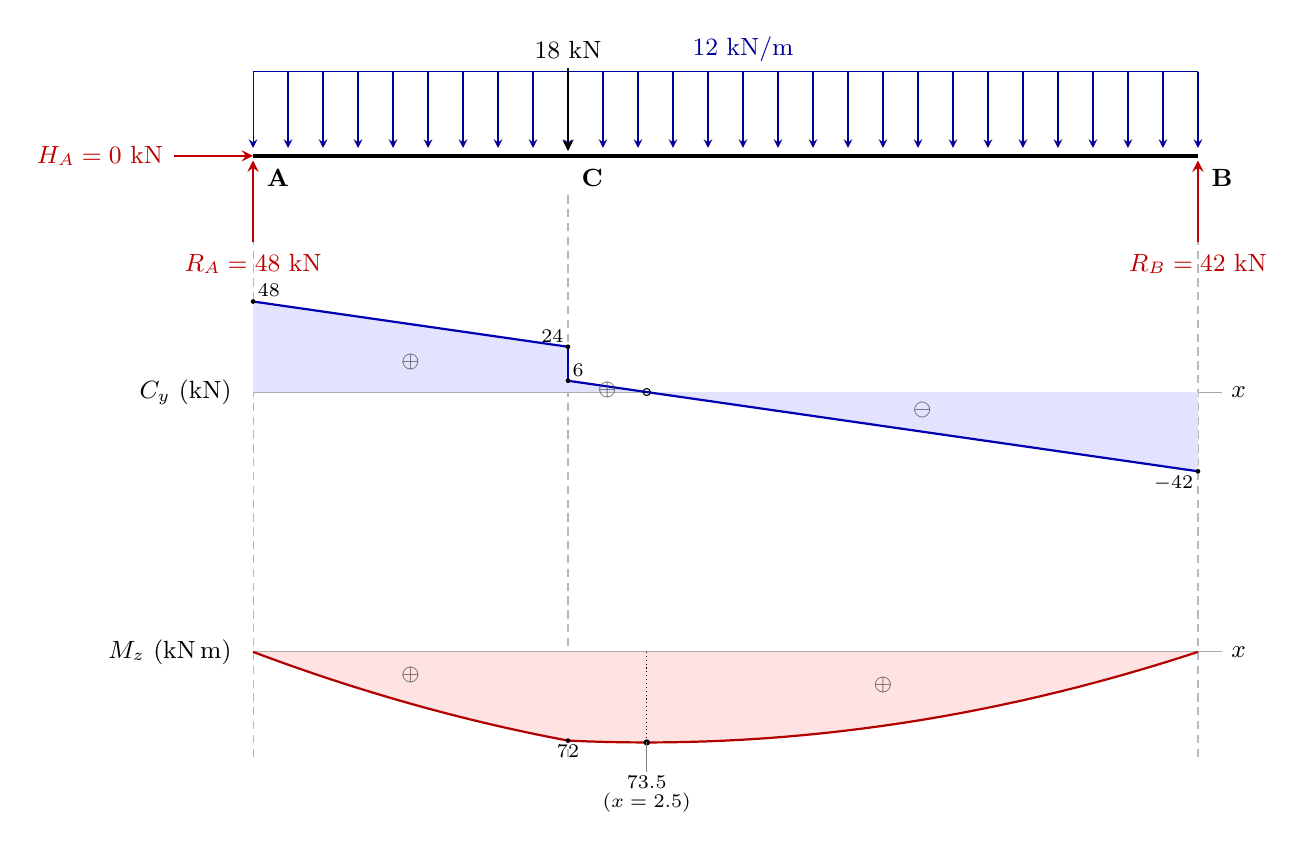
\begin{tikzpicture}
\draw[densely dashed,gray!55] (12.0000,-0.5000) -- (12.0000,-7.7000);
\draw[densely dashed,gray!55] (4.0000,-0.5000) -- (4.0000,-7.7000);
\draw[densely dashed,gray!55] (0.0000,-0.5000) -- (0.0000,-7.7000);
\draw[-stealth,blue!60!black] (0.0000,1.0700) -- (0.0000,0.1000);
\draw[-stealth,blue!60!black] (0.4444,1.0700) -- (0.4444,0.1000);
\draw[-stealth,blue!60!black] (0.8889,1.0700) -- (0.8889,0.1000);
\draw[-stealth,blue!60!black] (1.3333,1.0700) -- (1.3333,0.1000);
\draw[-stealth,blue!60!black] (1.7778,1.0700) -- (1.7778,0.1000);
\draw[-stealth,blue!60!black] (2.2222,1.0700) -- (2.2222,0.1000);
\draw[-stealth,blue!60!black] (2.6667,1.0700) -- (2.6667,0.1000);
\draw[-stealth,blue!60!black] (3.1111,1.0700) -- (3.1111,0.1000);
\draw[-stealth,blue!60!black] (3.5556,1.0700) -- (3.5556,0.1000);
\draw[-stealth,blue!60!black] (4.0000,1.0700) -- (4.0000,0.1000);
\draw[-stealth,blue!60!black] (4.4444,1.0700) -- (4.4444,0.1000);
\draw[-stealth,blue!60!black] (4.8889,1.0700) -- (4.8889,0.1000);
\draw[-stealth,blue!60!black] (5.3333,1.0700) -- (5.3333,0.1000);
\draw[-stealth,blue!60!black] (5.7778,1.0700) -- (5.7778,0.1000);
\draw[-stealth,blue!60!black] (6.2222,1.0700) -- (6.2222,0.1000);
\draw[-stealth,blue!60!black] (6.6667,1.0700) -- (6.6667,0.1000);
\draw[-stealth,blue!60!black] (7.1111,1.0700) -- (7.1111,0.1000);
\draw[-stealth,blue!60!black] (7.5556,1.0700) -- (7.5556,0.1000);
\draw[-stealth,blue!60!black] (8.0000,1.0700) -- (8.0000,0.1000);
\draw[-stealth,blue!60!black] (8.4444,1.0700) -- (8.4444,0.1000);
\draw[-stealth,blue!60!black] (8.8889,1.0700) -- (8.8889,0.1000);
\draw[-stealth,blue!60!black] (9.3333,1.0700) -- (9.3333,0.1000);
\draw[-stealth,blue!60!black] (9.7778,1.0700) -- (9.7778,0.1000);
\draw[-stealth,blue!60!black] (10.2222,1.0700) -- (10.2222,0.1000);
\draw[-stealth,blue!60!black] (10.6667,1.0700) -- (10.6667,0.1000);
\draw[-stealth,blue!60!black] (11.1111,1.0700) -- (11.1111,0.1000);
\draw[-stealth,blue!60!black] (11.5556,1.0700) -- (11.5556,0.1000);
\draw[-stealth,blue!60!black] (12.0000,1.0700) -- (12.0000,0.1000);
% studium:at distributed 0 x=0 to=6 check=span
\draw[blue!60!black] (0.0000,1.0700) -- (0.4444,1.0700) -- (0.8889,1.0700) -- (1.3333,1.0700) -- (1.7778,1.0700) -- (2.2222,1.0700) -- (2.6667,1.0700) -- (3.1111,1.0700) -- (3.5556,1.0700) -- (4.0000,1.0700) -- (4.4444,1.0700) -- (4.8889,1.0700) -- (5.3333,1.0700) -- (5.7778,1.0700) -- (6.2222,1.0700) -- (6.6667,1.0700) -- (7.1111,1.0700) -- (7.5556,1.0700) -- (8.0000,1.0700) -- (8.4444,1.0700) -- (8.8889,1.0700) -- (9.3333,1.0700) -- (9.7778,1.0700) -- (10.2222,1.0700) -- (10.6667,1.0700) -- (11.1111,1.0700) -- (11.5556,1.0700) -- (12.0000,1.0700);
\node[font=\small,anchor=south,blue!60!black] at (6.2222,1.0700) {$12$~\mbox{kN/m}};
\draw[line width=1.6pt] (0,0.0000) -- (12.0000,0.0000);
% studium:at force 0 x=2 check=tip
\draw[-stealth,thick,black] (4.0000,1.1100) -- (4.0000,0.0600);
\node[font=\small,anchor=south] at (4.0000,1.1100) {$18$~\mbox{kN}};
% studium:reaction H_A value=0
% studium:at reaction H_A x=0 check=tip
\draw[-stealth,thick,red!75!black] (-1.0000,0.0000) -- (0.0000,0.0000);
\node[font=\small,anchor=east,red!75!black] at (-1.0200,0.0000) {$H_{A} = 0$~\mbox{kN}};
% studium:reaction R_A value=48
% studium:at reaction R_A x=0 check=tip
\draw[-stealth,thick,red!75!black] (0.0000,-1.1000) -- (0.0000,-0.0600);
\node[font=\small,anchor=north,red!75!black] at (0.0000,-1.1200) {$R_{A} = 48$~\mbox{kN}};
% studium:reaction R_B value=42
% studium:at reaction R_B x=6 check=tip
\draw[-stealth,thick,red!75!black] (12.0000,-1.1000) -- (12.0000,-0.0600);
\node[font=\small,anchor=north,red!75!black] at (12.0000,-1.1200) {$R_{B} = 42$~\mbox{kN}};
\node[font=\small\bfseries,anchor=north west] at (0.0500,-0.0500) {A};
\node[font=\small\bfseries,anchor=north west] at (4.0500,-0.0500) {C};
\node[font=\small\bfseries,anchor=north west] at (12.0500,-0.0500) {B};
\draw[gray!70] (0,-3.0000) -- (12.3000,-3.0000);
\fill[blue!11] (0.0000,-3.0000) -- (0.0000,-1.8500) -- (4.0000,-2.4250) -- (4.0000,-3.0000) -- cycle;
\fill[blue!11] (4.0000,-3.0000) -- (4.0000,-2.8563) -- (12.0000,-4.0062) -- (12.0000,-3.0000) -- cycle;
% studium:series V sx=2.0 sy=0.02395833333333333 x0=0.0 y0=-3.0 sign=1
\draw[thick,blue!70!black] (0.0000,-1.8500) -- (4.0000,-2.4250);
\draw[thick,blue!70!black] (4.0000,-2.8563) -- (12.0000,-4.0062);
% studium:end V
\draw[thick,blue!70!black] (4.0000,-2.4250) -- (4.0000,-2.8563);
\node[font=\small,anchor=east] at (-0.15,-3.0000) {$C_y$ (kN)};
\node[font=\small,anchor=west] at (12.3000,-3.0000) {$x$};
% studium:label V x=0 side=right value=48
\fill (0.0000,-1.8500) circle (0.03);
\node[font=\scriptsize,anchor=south west,inner sep=1.5pt] at (0.0000,-1.8500) {$48$};
% studium:label V x=2 side=left value=24
\fill (4.0000,-2.4250) circle (0.03);
\node[font=\scriptsize,anchor=south east,inner sep=1.5pt] at (4.0000,-2.4250) {$24$};
% studium:label V x=2 side=right value=6
\fill (4.0000,-2.8563) circle (0.03);
\node[font=\scriptsize,anchor=south west,inner sep=1.5pt] at (4.0000,-2.8563) {$6$};
% studium:label V x=6 side=left value=-42
\fill (12.0000,-4.0062) circle (0.03);
\node[font=\scriptsize,anchor=north east,inner sep=1.5pt] at (12.0000,-4.0062) {$-42$};
\draw (5.0000,-3.0000) circle (0.045);
\node[font=\footnotesize,gray!60!black] at (2.0000,-2.6119) {$\oplus$};
\node[font=\footnotesize,gray!60!black] at (4.5000,-2.9677) {$\oplus$};
\node[font=\footnotesize,gray!60!black] at (8.5000,-3.2264) {$\ominus$};
\draw[gray!70] (0,-6.3000) -- (12.3000,-6.3000);
\fill[red!11] (0.0000,-6.3000) -- (0.0000,-6.3000) -- (0.1250,-6.3466) -- (0.2500,-6.3924) -- (0.3750,-6.4375) -- (0.5000,-6.4819) -- (0.6250,-6.5255) -- (0.7500,-6.5684) -- (0.8750,-6.6106) -- (1.0000,-6.6520) -- (1.1250,-6.6927) -- (1.2500,-6.7327) -- (1.3750,-6.7720) -- (1.5000,-6.8105) -- (1.6250,-6.8482) -- (1.7500,-6.8853) -- (1.8750,-6.9216) -- (2.0000,-6.9571) -- (2.1250,-6.9920) -- (2.2500,-7.0261) -- (2.3750,-7.0595) -- (2.5000,-7.0921) -- (2.6250,-7.1240) -- (2.7500,-7.1552) -- (2.8750,-7.1856) -- (3.0000,-7.2153) -- (3.1250,-7.2443) -- (3.2500,-7.2725) -- (3.3750,-7.3000) -- (3.5000,-7.3268) -- (3.6250,-7.3528) -- (3.7500,-7.3781) -- (3.8750,-7.4027) -- (4.0000,-7.4265) -- (4.0000,-6.3000) -- cycle;
\fill[red!11] (4.0000,-6.3000) -- (4.0000,-7.4265) -- (4.2500,-7.4368) -- (4.5000,-7.4441) -- (4.7500,-7.4485) -- (5.0000,-7.4500) -- (5.2500,-7.4485) -- (5.5000,-7.4441) -- (5.7500,-7.4368) -- (6.0000,-7.4265) -- (6.2500,-7.4133) -- (6.5000,-7.3972) -- (6.7500,-7.3781) -- (7.0000,-7.3561) -- (7.2500,-7.3312) -- (7.5000,-7.3033) -- (7.7500,-7.2725) -- (8.0000,-7.2388) -- (8.2500,-7.2021) -- (8.5000,-7.1625) -- (8.7500,-7.1200) -- (9.0000,-7.0745) -- (9.2500,-7.0261) -- (9.5000,-6.9747) -- (9.7500,-6.9205) -- (10.0000,-6.8633) -- (10.2500,-6.8031) -- (10.5000,-6.7401) -- (10.7500,-6.6740) -- (11.0000,-6.6051) -- (11.2500,-6.5332) -- (11.5000,-6.4584) -- (11.7500,-6.3807) -- (12.0000,-6.3000) -- (12.0000,-6.3000) -- cycle;
% studium:series M sx=2.0 sy=0.01564625850340136 x0=0.0 y0=-6.3 sign=-1
\draw[thick,red!70!black] (0.0000,-6.3000) -- (0.1250,-6.3466) -- (0.2500,-6.3924) -- (0.3750,-6.4375) -- (0.5000,-6.4819) -- (0.6250,-6.5255) -- (0.7500,-6.5684) -- (0.8750,-6.6106) -- (1.0000,-6.6520) -- (1.1250,-6.6927) -- (1.2500,-6.7327) -- (1.3750,-6.7720) -- (1.5000,-6.8105) -- (1.6250,-6.8482) -- (1.7500,-6.8853) -- (1.8750,-6.9216) -- (2.0000,-6.9571) -- (2.1250,-6.9920) -- (2.2500,-7.0261) -- (2.3750,-7.0595) -- (2.5000,-7.0921) -- (2.6250,-7.1240) -- (2.7500,-7.1552) -- (2.8750,-7.1856) -- (3.0000,-7.2153) -- (3.1250,-7.2443) -- (3.2500,-7.2725) -- (3.3750,-7.3000) -- (3.5000,-7.3268) -- (3.6250,-7.3528) -- (3.7500,-7.3781) -- (3.8750,-7.4027) -- (4.0000,-7.4265);
\draw[thick,red!70!black] (4.0000,-7.4265) -- (4.2500,-7.4368) -- (4.5000,-7.4441) -- (4.7500,-7.4485) -- (5.0000,-7.4500) -- (5.2500,-7.4485) -- (5.5000,-7.4441) -- (5.7500,-7.4368) -- (6.0000,-7.4265) -- (6.2500,-7.4133) -- (6.5000,-7.3972) -- (6.7500,-7.3781) -- (7.0000,-7.3561) -- (7.2500,-7.3312) -- (7.5000,-7.3033) -- (7.7500,-7.2725) -- (8.0000,-7.2388) -- (8.2500,-7.2021) -- (8.5000,-7.1625) -- (8.7500,-7.1200) -- (9.0000,-7.0745) -- (9.2500,-7.0261) -- (9.5000,-6.9747) -- (9.7500,-6.9205) -- (10.0000,-6.8633) -- (10.2500,-6.8031) -- (10.5000,-6.7401) -- (10.7500,-6.6740) -- (11.0000,-6.6051) -- (11.2500,-6.5332) -- (11.5000,-6.4584) -- (11.7500,-6.3807) -- (12.0000,-6.3000);
% studium:end M
\node[font=\small,anchor=east] at (-0.15,-6.3000) {$M_z$ (kN\,m)};
\node[font=\small,anchor=west] at (12.3000,-6.3000) {$x$};
% studium:label M x=2 side=both value=72
\fill (4.0000,-7.4265) circle (0.03);
\node[font=\scriptsize,anchor=north,inner sep=1.5pt] at (4.0000,-7.4265) {$72$};
% studium:label M x=5/2 side=both value=73.5
\fill (5.0000,-7.4500) circle (0.04);
\draw[densely dotted] (5.0000,-6.3000) -- (5.0000,-7.4500);
\draw[gray] (5.0000,-7.4500) -- (5.0000,-7.8300);
\node[font=\scriptsize,anchor=north,inner sep=1pt,align=center,fill=white,fill opacity=0.8,text opacity=1] at (5.0000,-7.8300) {$73.5$\\[-1pt]$(x = 2.5)$};
\node[font=\footnotesize,gray!60!black] at (2.0000,-6.5957) {$\oplus$};
\node[font=\footnotesize,gray!60!black] at (8.0000,-6.7224) {$\oplus$};
\end{tikzpicture}}%
\count0=\ht0
\advance\count0 by \dp0
\count2=\wd0
\count4=\dimexpr\textheight/100*38\relax
\count6=\linewidth
\ifnum\count0<1
\count0=1
\fi
\ifnum\count2<1
\count2=1
\fi
\divide\count0 by 4096
\divide\count2 by 4096
\divide\count4 by 4096
\divide\count6 by 4096
\ifnum\count0<1
\count0=1
\fi
\ifnum\count2<1
\count2=1
\fi
\ifnum\count4<1
\count4=1
\fi
\ifnum\count6<1
\count6=1
\fi
\count8=\count2
\ifnum\count0>\count4
\count8=\numexpr\count2*\count4/\count0\relax
\fi
\ifnum\count8>\count6
\resizebox{\linewidth}{!}{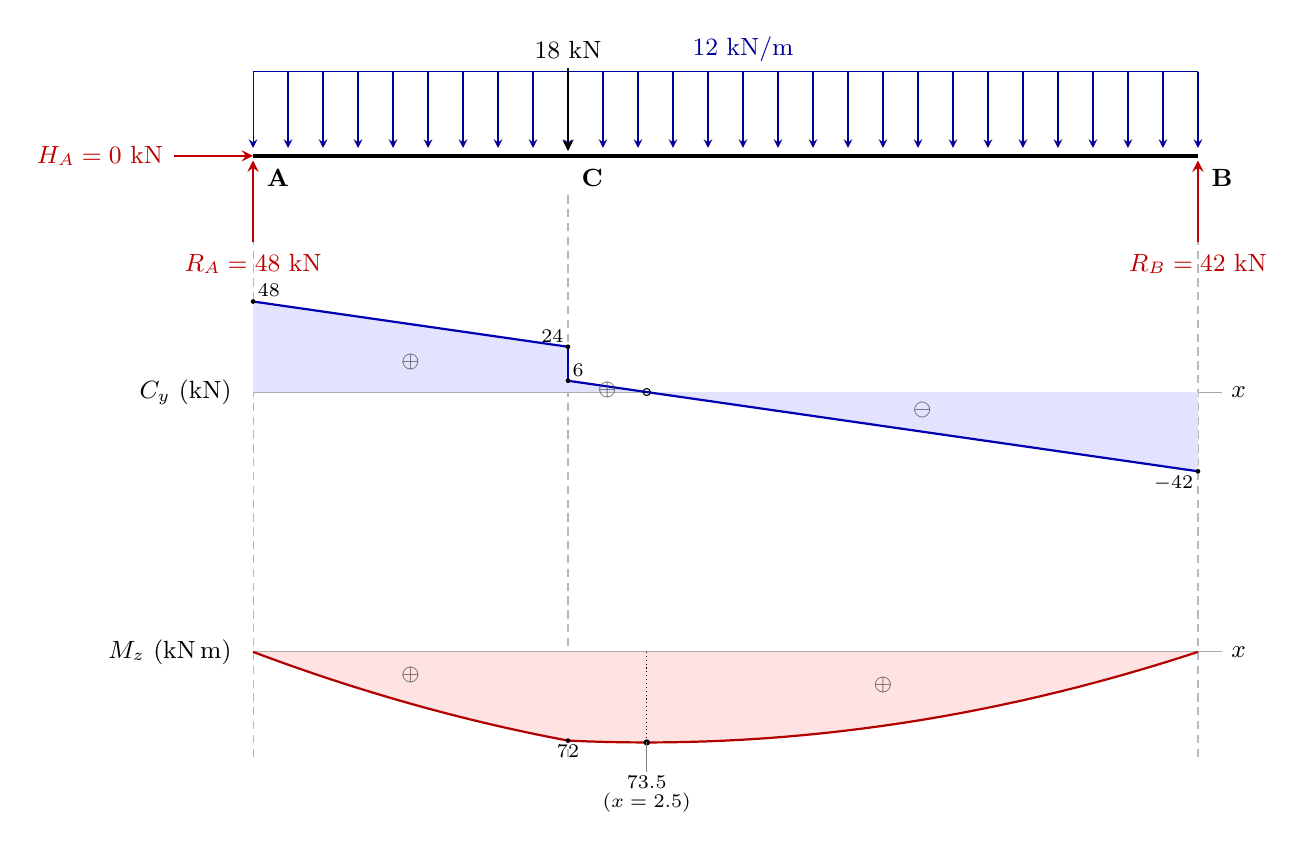
\begin{tikzpicture}
\draw[densely dashed,gray!55] (12.0000,-0.5000) -- (12.0000,-7.7000);
\draw[densely dashed,gray!55] (4.0000,-0.5000) -- (4.0000,-7.7000);
\draw[densely dashed,gray!55] (0.0000,-0.5000) -- (0.0000,-7.7000);
\draw[-stealth,blue!60!black] (0.0000,1.0700) -- (0.0000,0.1000);
\draw[-stealth,blue!60!black] (0.4444,1.0700) -- (0.4444,0.1000);
\draw[-stealth,blue!60!black] (0.8889,1.0700) -- (0.8889,0.1000);
\draw[-stealth,blue!60!black] (1.3333,1.0700) -- (1.3333,0.1000);
\draw[-stealth,blue!60!black] (1.7778,1.0700) -- (1.7778,0.1000);
\draw[-stealth,blue!60!black] (2.2222,1.0700) -- (2.2222,0.1000);
\draw[-stealth,blue!60!black] (2.6667,1.0700) -- (2.6667,0.1000);
\draw[-stealth,blue!60!black] (3.1111,1.0700) -- (3.1111,0.1000);
\draw[-stealth,blue!60!black] (3.5556,1.0700) -- (3.5556,0.1000);
\draw[-stealth,blue!60!black] (4.0000,1.0700) -- (4.0000,0.1000);
\draw[-stealth,blue!60!black] (4.4444,1.0700) -- (4.4444,0.1000);
\draw[-stealth,blue!60!black] (4.8889,1.0700) -- (4.8889,0.1000);
\draw[-stealth,blue!60!black] (5.3333,1.0700) -- (5.3333,0.1000);
\draw[-stealth,blue!60!black] (5.7778,1.0700) -- (5.7778,0.1000);
\draw[-stealth,blue!60!black] (6.2222,1.0700) -- (6.2222,0.1000);
\draw[-stealth,blue!60!black] (6.6667,1.0700) -- (6.6667,0.1000);
\draw[-stealth,blue!60!black] (7.1111,1.0700) -- (7.1111,0.1000);
\draw[-stealth,blue!60!black] (7.5556,1.0700) -- (7.5556,0.1000);
\draw[-stealth,blue!60!black] (8.0000,1.0700) -- (8.0000,0.1000);
\draw[-stealth,blue!60!black] (8.4444,1.0700) -- (8.4444,0.1000);
\draw[-stealth,blue!60!black] (8.8889,1.0700) -- (8.8889,0.1000);
\draw[-stealth,blue!60!black] (9.3333,1.0700) -- (9.3333,0.1000);
\draw[-stealth,blue!60!black] (9.7778,1.0700) -- (9.7778,0.1000);
\draw[-stealth,blue!60!black] (10.2222,1.0700) -- (10.2222,0.1000);
\draw[-stealth,blue!60!black] (10.6667,1.0700) -- (10.6667,0.1000);
\draw[-stealth,blue!60!black] (11.1111,1.0700) -- (11.1111,0.1000);
\draw[-stealth,blue!60!black] (11.5556,1.0700) -- (11.5556,0.1000);
\draw[-stealth,blue!60!black] (12.0000,1.0700) -- (12.0000,0.1000);
% studium:at distributed 0 x=0 to=6 check=span
\draw[blue!60!black] (0.0000,1.0700) -- (0.4444,1.0700) -- (0.8889,1.0700) -- (1.3333,1.0700) -- (1.7778,1.0700) -- (2.2222,1.0700) -- (2.6667,1.0700) -- (3.1111,1.0700) -- (3.5556,1.0700) -- (4.0000,1.0700) -- (4.4444,1.0700) -- (4.8889,1.0700) -- (5.3333,1.0700) -- (5.7778,1.0700) -- (6.2222,1.0700) -- (6.6667,1.0700) -- (7.1111,1.0700) -- (7.5556,1.0700) -- (8.0000,1.0700) -- (8.4444,1.0700) -- (8.8889,1.0700) -- (9.3333,1.0700) -- (9.7778,1.0700) -- (10.2222,1.0700) -- (10.6667,1.0700) -- (11.1111,1.0700) -- (11.5556,1.0700) -- (12.0000,1.0700);
\node[font=\small,anchor=south,blue!60!black] at (6.2222,1.0700) {$12$~\mbox{kN/m}};
\draw[line width=1.6pt] (0,0.0000) -- (12.0000,0.0000);
% studium:at force 0 x=2 check=tip
\draw[-stealth,thick,black] (4.0000,1.1100) -- (4.0000,0.0600);
\node[font=\small,anchor=south] at (4.0000,1.1100) {$18$~\mbox{kN}};
% studium:reaction H_A value=0
% studium:at reaction H_A x=0 check=tip
\draw[-stealth,thick,red!75!black] (-1.0000,0.0000) -- (0.0000,0.0000);
\node[font=\small,anchor=east,red!75!black] at (-1.0200,0.0000) {$H_{A} = 0$~\mbox{kN}};
% studium:reaction R_A value=48
% studium:at reaction R_A x=0 check=tip
\draw[-stealth,thick,red!75!black] (0.0000,-1.1000) -- (0.0000,-0.0600);
\node[font=\small,anchor=north,red!75!black] at (0.0000,-1.1200) {$R_{A} = 48$~\mbox{kN}};
% studium:reaction R_B value=42
% studium:at reaction R_B x=6 check=tip
\draw[-stealth,thick,red!75!black] (12.0000,-1.1000) -- (12.0000,-0.0600);
\node[font=\small,anchor=north,red!75!black] at (12.0000,-1.1200) {$R_{B} = 42$~\mbox{kN}};
\node[font=\small\bfseries,anchor=north west] at (0.0500,-0.0500) {A};
\node[font=\small\bfseries,anchor=north west] at (4.0500,-0.0500) {C};
\node[font=\small\bfseries,anchor=north west] at (12.0500,-0.0500) {B};
\draw[gray!70] (0,-3.0000) -- (12.3000,-3.0000);
\fill[blue!11] (0.0000,-3.0000) -- (0.0000,-1.8500) -- (4.0000,-2.4250) -- (4.0000,-3.0000) -- cycle;
\fill[blue!11] (4.0000,-3.0000) -- (4.0000,-2.8563) -- (12.0000,-4.0062) -- (12.0000,-3.0000) -- cycle;
% studium:series V sx=2.0 sy=0.02395833333333333 x0=0.0 y0=-3.0 sign=1
\draw[thick,blue!70!black] (0.0000,-1.8500) -- (4.0000,-2.4250);
\draw[thick,blue!70!black] (4.0000,-2.8563) -- (12.0000,-4.0062);
% studium:end V
\draw[thick,blue!70!black] (4.0000,-2.4250) -- (4.0000,-2.8563);
\node[font=\small,anchor=east] at (-0.15,-3.0000) {$C_y$ (kN)};
\node[font=\small,anchor=west] at (12.3000,-3.0000) {$x$};
% studium:label V x=0 side=right value=48
\fill (0.0000,-1.8500) circle (0.03);
\node[font=\scriptsize,anchor=south west,inner sep=1.5pt] at (0.0000,-1.8500) {$48$};
% studium:label V x=2 side=left value=24
\fill (4.0000,-2.4250) circle (0.03);
\node[font=\scriptsize,anchor=south east,inner sep=1.5pt] at (4.0000,-2.4250) {$24$};
% studium:label V x=2 side=right value=6
\fill (4.0000,-2.8563) circle (0.03);
\node[font=\scriptsize,anchor=south west,inner sep=1.5pt] at (4.0000,-2.8563) {$6$};
% studium:label V x=6 side=left value=-42
\fill (12.0000,-4.0062) circle (0.03);
\node[font=\scriptsize,anchor=north east,inner sep=1.5pt] at (12.0000,-4.0062) {$-42$};
\draw (5.0000,-3.0000) circle (0.045);
\node[font=\footnotesize,gray!60!black] at (2.0000,-2.6119) {$\oplus$};
\node[font=\footnotesize,gray!60!black] at (4.5000,-2.9677) {$\oplus$};
\node[font=\footnotesize,gray!60!black] at (8.5000,-3.2264) {$\ominus$};
\draw[gray!70] (0,-6.3000) -- (12.3000,-6.3000);
\fill[red!11] (0.0000,-6.3000) -- (0.0000,-6.3000) -- (0.1250,-6.3466) -- (0.2500,-6.3924) -- (0.3750,-6.4375) -- (0.5000,-6.4819) -- (0.6250,-6.5255) -- (0.7500,-6.5684) -- (0.8750,-6.6106) -- (1.0000,-6.6520) -- (1.1250,-6.6927) -- (1.2500,-6.7327) -- (1.3750,-6.7720) -- (1.5000,-6.8105) -- (1.6250,-6.8482) -- (1.7500,-6.8853) -- (1.8750,-6.9216) -- (2.0000,-6.9571) -- (2.1250,-6.9920) -- (2.2500,-7.0261) -- (2.3750,-7.0595) -- (2.5000,-7.0921) -- (2.6250,-7.1240) -- (2.7500,-7.1552) -- (2.8750,-7.1856) -- (3.0000,-7.2153) -- (3.1250,-7.2443) -- (3.2500,-7.2725) -- (3.3750,-7.3000) -- (3.5000,-7.3268) -- (3.6250,-7.3528) -- (3.7500,-7.3781) -- (3.8750,-7.4027) -- (4.0000,-7.4265) -- (4.0000,-6.3000) -- cycle;
\fill[red!11] (4.0000,-6.3000) -- (4.0000,-7.4265) -- (4.2500,-7.4368) -- (4.5000,-7.4441) -- (4.7500,-7.4485) -- (5.0000,-7.4500) -- (5.2500,-7.4485) -- (5.5000,-7.4441) -- (5.7500,-7.4368) -- (6.0000,-7.4265) -- (6.2500,-7.4133) -- (6.5000,-7.3972) -- (6.7500,-7.3781) -- (7.0000,-7.3561) -- (7.2500,-7.3312) -- (7.5000,-7.3033) -- (7.7500,-7.2725) -- (8.0000,-7.2388) -- (8.2500,-7.2021) -- (8.5000,-7.1625) -- (8.7500,-7.1200) -- (9.0000,-7.0745) -- (9.2500,-7.0261) -- (9.5000,-6.9747) -- (9.7500,-6.9205) -- (10.0000,-6.8633) -- (10.2500,-6.8031) -- (10.5000,-6.7401) -- (10.7500,-6.6740) -- (11.0000,-6.6051) -- (11.2500,-6.5332) -- (11.5000,-6.4584) -- (11.7500,-6.3807) -- (12.0000,-6.3000) -- (12.0000,-6.3000) -- cycle;
% studium:series M sx=2.0 sy=0.01564625850340136 x0=0.0 y0=-6.3 sign=-1
\draw[thick,red!70!black] (0.0000,-6.3000) -- (0.1250,-6.3466) -- (0.2500,-6.3924) -- (0.3750,-6.4375) -- (0.5000,-6.4819) -- (0.6250,-6.5255) -- (0.7500,-6.5684) -- (0.8750,-6.6106) -- (1.0000,-6.6520) -- (1.1250,-6.6927) -- (1.2500,-6.7327) -- (1.3750,-6.7720) -- (1.5000,-6.8105) -- (1.6250,-6.8482) -- (1.7500,-6.8853) -- (1.8750,-6.9216) -- (2.0000,-6.9571) -- (2.1250,-6.9920) -- (2.2500,-7.0261) -- (2.3750,-7.0595) -- (2.5000,-7.0921) -- (2.6250,-7.1240) -- (2.7500,-7.1552) -- (2.8750,-7.1856) -- (3.0000,-7.2153) -- (3.1250,-7.2443) -- (3.2500,-7.2725) -- (3.3750,-7.3000) -- (3.5000,-7.3268) -- (3.6250,-7.3528) -- (3.7500,-7.3781) -- (3.8750,-7.4027) -- (4.0000,-7.4265);
\draw[thick,red!70!black] (4.0000,-7.4265) -- (4.2500,-7.4368) -- (4.5000,-7.4441) -- (4.7500,-7.4485) -- (5.0000,-7.4500) -- (5.2500,-7.4485) -- (5.5000,-7.4441) -- (5.7500,-7.4368) -- (6.0000,-7.4265) -- (6.2500,-7.4133) -- (6.5000,-7.3972) -- (6.7500,-7.3781) -- (7.0000,-7.3561) -- (7.2500,-7.3312) -- (7.5000,-7.3033) -- (7.7500,-7.2725) -- (8.0000,-7.2388) -- (8.2500,-7.2021) -- (8.5000,-7.1625) -- (8.7500,-7.1200) -- (9.0000,-7.0745) -- (9.2500,-7.0261) -- (9.5000,-6.9747) -- (9.7500,-6.9205) -- (10.0000,-6.8633) -- (10.2500,-6.8031) -- (10.5000,-6.7401) -- (10.7500,-6.6740) -- (11.0000,-6.6051) -- (11.2500,-6.5332) -- (11.5000,-6.4584) -- (11.7500,-6.3807) -- (12.0000,-6.3000);
% studium:end M
\node[font=\small,anchor=east] at (-0.15,-6.3000) {$M_z$ (kN\,m)};
\node[font=\small,anchor=west] at (12.3000,-6.3000) {$x$};
% studium:label M x=2 side=both value=72
\fill (4.0000,-7.4265) circle (0.03);
\node[font=\scriptsize,anchor=north,inner sep=1.5pt] at (4.0000,-7.4265) {$72$};
% studium:label M x=5/2 side=both value=73.5
\fill (5.0000,-7.4500) circle (0.04);
\draw[densely dotted] (5.0000,-6.3000) -- (5.0000,-7.4500);
\draw[gray] (5.0000,-7.4500) -- (5.0000,-7.8300);
\node[font=\scriptsize,anchor=north,inner sep=1pt,align=center,fill=white,fill opacity=0.8,text opacity=1] at (5.0000,-7.8300) {$73.5$\\[-1pt]$(x = 2.5)$};
\node[font=\footnotesize,gray!60!black] at (2.0000,-6.5957) {$\oplus$};
\node[font=\footnotesize,gray!60!black] at (8.0000,-6.7224) {$\oplus$};
\end{tikzpicture}}%
\else
\ifnum\count0>\count4
\resizebox{!}{\dimexpr\textheight/100*38\relax}{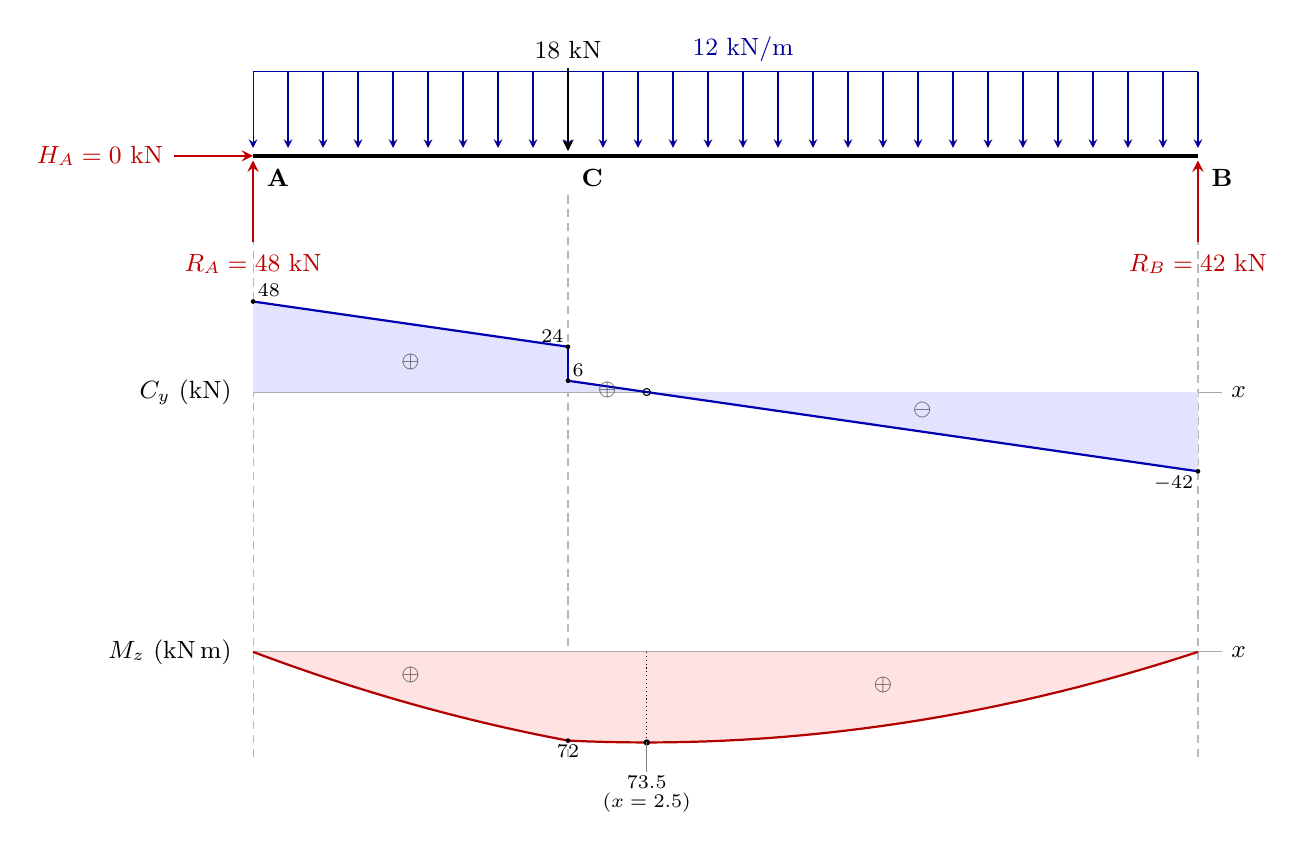
\begin{tikzpicture}
\draw[densely dashed,gray!55] (12.0000,-0.5000) -- (12.0000,-7.7000);
\draw[densely dashed,gray!55] (4.0000,-0.5000) -- (4.0000,-7.7000);
\draw[densely dashed,gray!55] (0.0000,-0.5000) -- (0.0000,-7.7000);
\draw[-stealth,blue!60!black] (0.0000,1.0700) -- (0.0000,0.1000);
\draw[-stealth,blue!60!black] (0.4444,1.0700) -- (0.4444,0.1000);
\draw[-stealth,blue!60!black] (0.8889,1.0700) -- (0.8889,0.1000);
\draw[-stealth,blue!60!black] (1.3333,1.0700) -- (1.3333,0.1000);
\draw[-stealth,blue!60!black] (1.7778,1.0700) -- (1.7778,0.1000);
\draw[-stealth,blue!60!black] (2.2222,1.0700) -- (2.2222,0.1000);
\draw[-stealth,blue!60!black] (2.6667,1.0700) -- (2.6667,0.1000);
\draw[-stealth,blue!60!black] (3.1111,1.0700) -- (3.1111,0.1000);
\draw[-stealth,blue!60!black] (3.5556,1.0700) -- (3.5556,0.1000);
\draw[-stealth,blue!60!black] (4.0000,1.0700) -- (4.0000,0.1000);
\draw[-stealth,blue!60!black] (4.4444,1.0700) -- (4.4444,0.1000);
\draw[-stealth,blue!60!black] (4.8889,1.0700) -- (4.8889,0.1000);
\draw[-stealth,blue!60!black] (5.3333,1.0700) -- (5.3333,0.1000);
\draw[-stealth,blue!60!black] (5.7778,1.0700) -- (5.7778,0.1000);
\draw[-stealth,blue!60!black] (6.2222,1.0700) -- (6.2222,0.1000);
\draw[-stealth,blue!60!black] (6.6667,1.0700) -- (6.6667,0.1000);
\draw[-stealth,blue!60!black] (7.1111,1.0700) -- (7.1111,0.1000);
\draw[-stealth,blue!60!black] (7.5556,1.0700) -- (7.5556,0.1000);
\draw[-stealth,blue!60!black] (8.0000,1.0700) -- (8.0000,0.1000);
\draw[-stealth,blue!60!black] (8.4444,1.0700) -- (8.4444,0.1000);
\draw[-stealth,blue!60!black] (8.8889,1.0700) -- (8.8889,0.1000);
\draw[-stealth,blue!60!black] (9.3333,1.0700) -- (9.3333,0.1000);
\draw[-stealth,blue!60!black] (9.7778,1.0700) -- (9.7778,0.1000);
\draw[-stealth,blue!60!black] (10.2222,1.0700) -- (10.2222,0.1000);
\draw[-stealth,blue!60!black] (10.6667,1.0700) -- (10.6667,0.1000);
\draw[-stealth,blue!60!black] (11.1111,1.0700) -- (11.1111,0.1000);
\draw[-stealth,blue!60!black] (11.5556,1.0700) -- (11.5556,0.1000);
\draw[-stealth,blue!60!black] (12.0000,1.0700) -- (12.0000,0.1000);
% studium:at distributed 0 x=0 to=6 check=span
\draw[blue!60!black] (0.0000,1.0700) -- (0.4444,1.0700) -- (0.8889,1.0700) -- (1.3333,1.0700) -- (1.7778,1.0700) -- (2.2222,1.0700) -- (2.6667,1.0700) -- (3.1111,1.0700) -- (3.5556,1.0700) -- (4.0000,1.0700) -- (4.4444,1.0700) -- (4.8889,1.0700) -- (5.3333,1.0700) -- (5.7778,1.0700) -- (6.2222,1.0700) -- (6.6667,1.0700) -- (7.1111,1.0700) -- (7.5556,1.0700) -- (8.0000,1.0700) -- (8.4444,1.0700) -- (8.8889,1.0700) -- (9.3333,1.0700) -- (9.7778,1.0700) -- (10.2222,1.0700) -- (10.6667,1.0700) -- (11.1111,1.0700) -- (11.5556,1.0700) -- (12.0000,1.0700);
\node[font=\small,anchor=south,blue!60!black] at (6.2222,1.0700) {$12$~\mbox{kN/m}};
\draw[line width=1.6pt] (0,0.0000) -- (12.0000,0.0000);
% studium:at force 0 x=2 check=tip
\draw[-stealth,thick,black] (4.0000,1.1100) -- (4.0000,0.0600);
\node[font=\small,anchor=south] at (4.0000,1.1100) {$18$~\mbox{kN}};
% studium:reaction H_A value=0
% studium:at reaction H_A x=0 check=tip
\draw[-stealth,thick,red!75!black] (-1.0000,0.0000) -- (0.0000,0.0000);
\node[font=\small,anchor=east,red!75!black] at (-1.0200,0.0000) {$H_{A} = 0$~\mbox{kN}};
% studium:reaction R_A value=48
% studium:at reaction R_A x=0 check=tip
\draw[-stealth,thick,red!75!black] (0.0000,-1.1000) -- (0.0000,-0.0600);
\node[font=\small,anchor=north,red!75!black] at (0.0000,-1.1200) {$R_{A} = 48$~\mbox{kN}};
% studium:reaction R_B value=42
% studium:at reaction R_B x=6 check=tip
\draw[-stealth,thick,red!75!black] (12.0000,-1.1000) -- (12.0000,-0.0600);
\node[font=\small,anchor=north,red!75!black] at (12.0000,-1.1200) {$R_{B} = 42$~\mbox{kN}};
\node[font=\small\bfseries,anchor=north west] at (0.0500,-0.0500) {A};
\node[font=\small\bfseries,anchor=north west] at (4.0500,-0.0500) {C};
\node[font=\small\bfseries,anchor=north west] at (12.0500,-0.0500) {B};
\draw[gray!70] (0,-3.0000) -- (12.3000,-3.0000);
\fill[blue!11] (0.0000,-3.0000) -- (0.0000,-1.8500) -- (4.0000,-2.4250) -- (4.0000,-3.0000) -- cycle;
\fill[blue!11] (4.0000,-3.0000) -- (4.0000,-2.8563) -- (12.0000,-4.0062) -- (12.0000,-3.0000) -- cycle;
% studium:series V sx=2.0 sy=0.02395833333333333 x0=0.0 y0=-3.0 sign=1
\draw[thick,blue!70!black] (0.0000,-1.8500) -- (4.0000,-2.4250);
\draw[thick,blue!70!black] (4.0000,-2.8563) -- (12.0000,-4.0062);
% studium:end V
\draw[thick,blue!70!black] (4.0000,-2.4250) -- (4.0000,-2.8563);
\node[font=\small,anchor=east] at (-0.15,-3.0000) {$C_y$ (kN)};
\node[font=\small,anchor=west] at (12.3000,-3.0000) {$x$};
% studium:label V x=0 side=right value=48
\fill (0.0000,-1.8500) circle (0.03);
\node[font=\scriptsize,anchor=south west,inner sep=1.5pt] at (0.0000,-1.8500) {$48$};
% studium:label V x=2 side=left value=24
\fill (4.0000,-2.4250) circle (0.03);
\node[font=\scriptsize,anchor=south east,inner sep=1.5pt] at (4.0000,-2.4250) {$24$};
% studium:label V x=2 side=right value=6
\fill (4.0000,-2.8563) circle (0.03);
\node[font=\scriptsize,anchor=south west,inner sep=1.5pt] at (4.0000,-2.8563) {$6$};
% studium:label V x=6 side=left value=-42
\fill (12.0000,-4.0062) circle (0.03);
\node[font=\scriptsize,anchor=north east,inner sep=1.5pt] at (12.0000,-4.0062) {$-42$};
\draw (5.0000,-3.0000) circle (0.045);
\node[font=\footnotesize,gray!60!black] at (2.0000,-2.6119) {$\oplus$};
\node[font=\footnotesize,gray!60!black] at (4.5000,-2.9677) {$\oplus$};
\node[font=\footnotesize,gray!60!black] at (8.5000,-3.2264) {$\ominus$};
\draw[gray!70] (0,-6.3000) -- (12.3000,-6.3000);
\fill[red!11] (0.0000,-6.3000) -- (0.0000,-6.3000) -- (0.1250,-6.3466) -- (0.2500,-6.3924) -- (0.3750,-6.4375) -- (0.5000,-6.4819) -- (0.6250,-6.5255) -- (0.7500,-6.5684) -- (0.8750,-6.6106) -- (1.0000,-6.6520) -- (1.1250,-6.6927) -- (1.2500,-6.7327) -- (1.3750,-6.7720) -- (1.5000,-6.8105) -- (1.6250,-6.8482) -- (1.7500,-6.8853) -- (1.8750,-6.9216) -- (2.0000,-6.9571) -- (2.1250,-6.9920) -- (2.2500,-7.0261) -- (2.3750,-7.0595) -- (2.5000,-7.0921) -- (2.6250,-7.1240) -- (2.7500,-7.1552) -- (2.8750,-7.1856) -- (3.0000,-7.2153) -- (3.1250,-7.2443) -- (3.2500,-7.2725) -- (3.3750,-7.3000) -- (3.5000,-7.3268) -- (3.6250,-7.3528) -- (3.7500,-7.3781) -- (3.8750,-7.4027) -- (4.0000,-7.4265) -- (4.0000,-6.3000) -- cycle;
\fill[red!11] (4.0000,-6.3000) -- (4.0000,-7.4265) -- (4.2500,-7.4368) -- (4.5000,-7.4441) -- (4.7500,-7.4485) -- (5.0000,-7.4500) -- (5.2500,-7.4485) -- (5.5000,-7.4441) -- (5.7500,-7.4368) -- (6.0000,-7.4265) -- (6.2500,-7.4133) -- (6.5000,-7.3972) -- (6.7500,-7.3781) -- (7.0000,-7.3561) -- (7.2500,-7.3312) -- (7.5000,-7.3033) -- (7.7500,-7.2725) -- (8.0000,-7.2388) -- (8.2500,-7.2021) -- (8.5000,-7.1625) -- (8.7500,-7.1200) -- (9.0000,-7.0745) -- (9.2500,-7.0261) -- (9.5000,-6.9747) -- (9.7500,-6.9205) -- (10.0000,-6.8633) -- (10.2500,-6.8031) -- (10.5000,-6.7401) -- (10.7500,-6.6740) -- (11.0000,-6.6051) -- (11.2500,-6.5332) -- (11.5000,-6.4584) -- (11.7500,-6.3807) -- (12.0000,-6.3000) -- (12.0000,-6.3000) -- cycle;
% studium:series M sx=2.0 sy=0.01564625850340136 x0=0.0 y0=-6.3 sign=-1
\draw[thick,red!70!black] (0.0000,-6.3000) -- (0.1250,-6.3466) -- (0.2500,-6.3924) -- (0.3750,-6.4375) -- (0.5000,-6.4819) -- (0.6250,-6.5255) -- (0.7500,-6.5684) -- (0.8750,-6.6106) -- (1.0000,-6.6520) -- (1.1250,-6.6927) -- (1.2500,-6.7327) -- (1.3750,-6.7720) -- (1.5000,-6.8105) -- (1.6250,-6.8482) -- (1.7500,-6.8853) -- (1.8750,-6.9216) -- (2.0000,-6.9571) -- (2.1250,-6.9920) -- (2.2500,-7.0261) -- (2.3750,-7.0595) -- (2.5000,-7.0921) -- (2.6250,-7.1240) -- (2.7500,-7.1552) -- (2.8750,-7.1856) -- (3.0000,-7.2153) -- (3.1250,-7.2443) -- (3.2500,-7.2725) -- (3.3750,-7.3000) -- (3.5000,-7.3268) -- (3.6250,-7.3528) -- (3.7500,-7.3781) -- (3.8750,-7.4027) -- (4.0000,-7.4265);
\draw[thick,red!70!black] (4.0000,-7.4265) -- (4.2500,-7.4368) -- (4.5000,-7.4441) -- (4.7500,-7.4485) -- (5.0000,-7.4500) -- (5.2500,-7.4485) -- (5.5000,-7.4441) -- (5.7500,-7.4368) -- (6.0000,-7.4265) -- (6.2500,-7.4133) -- (6.5000,-7.3972) -- (6.7500,-7.3781) -- (7.0000,-7.3561) -- (7.2500,-7.3312) -- (7.5000,-7.3033) -- (7.7500,-7.2725) -- (8.0000,-7.2388) -- (8.2500,-7.2021) -- (8.5000,-7.1625) -- (8.7500,-7.1200) -- (9.0000,-7.0745) -- (9.2500,-7.0261) -- (9.5000,-6.9747) -- (9.7500,-6.9205) -- (10.0000,-6.8633) -- (10.2500,-6.8031) -- (10.5000,-6.7401) -- (10.7500,-6.6740) -- (11.0000,-6.6051) -- (11.2500,-6.5332) -- (11.5000,-6.4584) -- (11.7500,-6.3807) -- (12.0000,-6.3000);
% studium:end M
\node[font=\small,anchor=east] at (-0.15,-6.3000) {$M_z$ (kN\,m)};
\node[font=\small,anchor=west] at (12.3000,-6.3000) {$x$};
% studium:label M x=2 side=both value=72
\fill (4.0000,-7.4265) circle (0.03);
\node[font=\scriptsize,anchor=north,inner sep=1.5pt] at (4.0000,-7.4265) {$72$};
% studium:label M x=5/2 side=both value=73.5
\fill (5.0000,-7.4500) circle (0.04);
\draw[densely dotted] (5.0000,-6.3000) -- (5.0000,-7.4500);
\draw[gray] (5.0000,-7.4500) -- (5.0000,-7.8300);
\node[font=\scriptsize,anchor=north,inner sep=1pt,align=center,fill=white,fill opacity=0.8,text opacity=1] at (5.0000,-7.8300) {$73.5$\\[-1pt]$(x = 2.5)$};
\node[font=\footnotesize,gray!60!black] at (2.0000,-6.5957) {$\oplus$};
\node[font=\footnotesize,gray!60!black] at (8.0000,-6.7224) {$\oplus$};
\end{tikzpicture}}%
\else
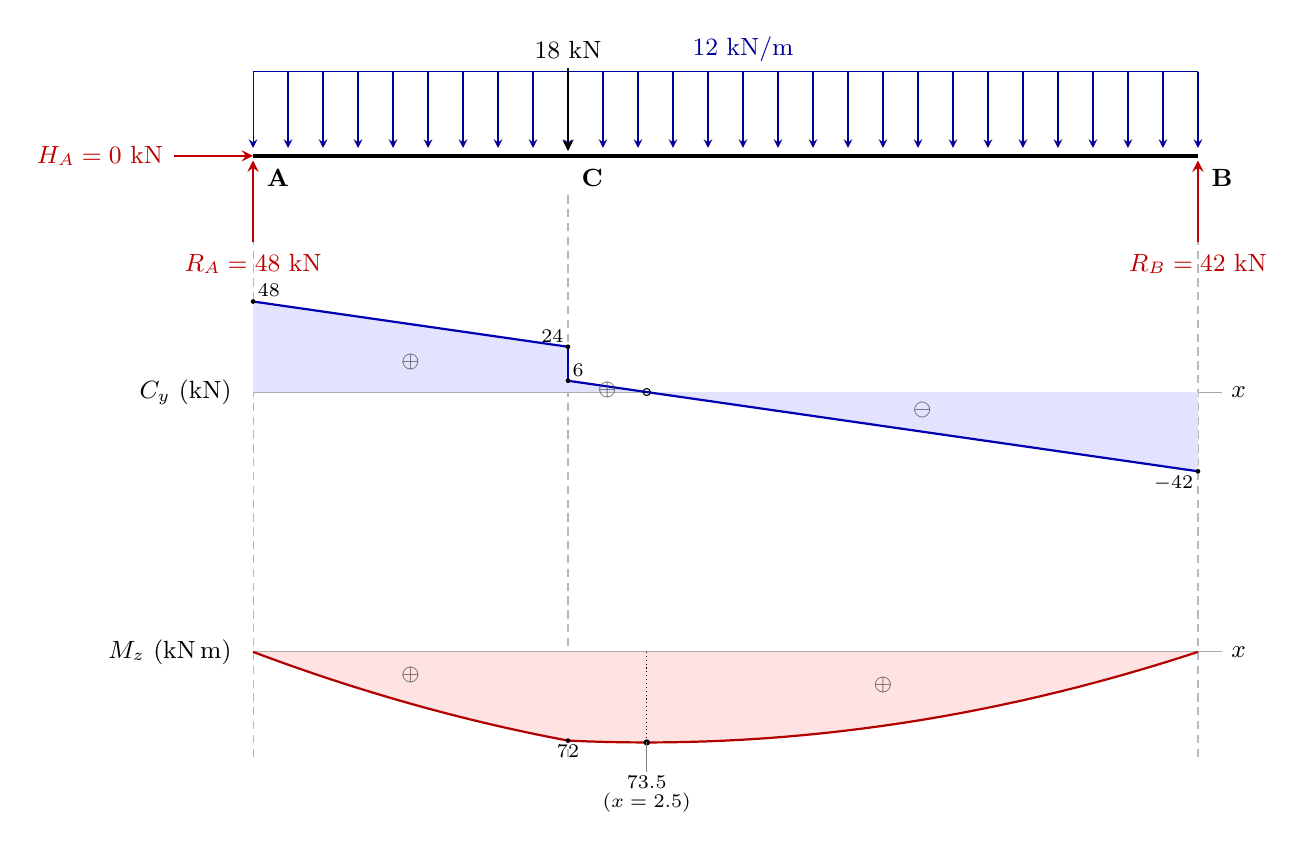
\begin{tikzpicture}
\draw[densely dashed,gray!55] (12.0000,-0.5000) -- (12.0000,-7.7000);
\draw[densely dashed,gray!55] (4.0000,-0.5000) -- (4.0000,-7.7000);
\draw[densely dashed,gray!55] (0.0000,-0.5000) -- (0.0000,-7.7000);
\draw[-stealth,blue!60!black] (0.0000,1.0700) -- (0.0000,0.1000);
\draw[-stealth,blue!60!black] (0.4444,1.0700) -- (0.4444,0.1000);
\draw[-stealth,blue!60!black] (0.8889,1.0700) -- (0.8889,0.1000);
\draw[-stealth,blue!60!black] (1.3333,1.0700) -- (1.3333,0.1000);
\draw[-stealth,blue!60!black] (1.7778,1.0700) -- (1.7778,0.1000);
\draw[-stealth,blue!60!black] (2.2222,1.0700) -- (2.2222,0.1000);
\draw[-stealth,blue!60!black] (2.6667,1.0700) -- (2.6667,0.1000);
\draw[-stealth,blue!60!black] (3.1111,1.0700) -- (3.1111,0.1000);
\draw[-stealth,blue!60!black] (3.5556,1.0700) -- (3.5556,0.1000);
\draw[-stealth,blue!60!black] (4.0000,1.0700) -- (4.0000,0.1000);
\draw[-stealth,blue!60!black] (4.4444,1.0700) -- (4.4444,0.1000);
\draw[-stealth,blue!60!black] (4.8889,1.0700) -- (4.8889,0.1000);
\draw[-stealth,blue!60!black] (5.3333,1.0700) -- (5.3333,0.1000);
\draw[-stealth,blue!60!black] (5.7778,1.0700) -- (5.7778,0.1000);
\draw[-stealth,blue!60!black] (6.2222,1.0700) -- (6.2222,0.1000);
\draw[-stealth,blue!60!black] (6.6667,1.0700) -- (6.6667,0.1000);
\draw[-stealth,blue!60!black] (7.1111,1.0700) -- (7.1111,0.1000);
\draw[-stealth,blue!60!black] (7.5556,1.0700) -- (7.5556,0.1000);
\draw[-stealth,blue!60!black] (8.0000,1.0700) -- (8.0000,0.1000);
\draw[-stealth,blue!60!black] (8.4444,1.0700) -- (8.4444,0.1000);
\draw[-stealth,blue!60!black] (8.8889,1.0700) -- (8.8889,0.1000);
\draw[-stealth,blue!60!black] (9.3333,1.0700) -- (9.3333,0.1000);
\draw[-stealth,blue!60!black] (9.7778,1.0700) -- (9.7778,0.1000);
\draw[-stealth,blue!60!black] (10.2222,1.0700) -- (10.2222,0.1000);
\draw[-stealth,blue!60!black] (10.6667,1.0700) -- (10.6667,0.1000);
\draw[-stealth,blue!60!black] (11.1111,1.0700) -- (11.1111,0.1000);
\draw[-stealth,blue!60!black] (11.5556,1.0700) -- (11.5556,0.1000);
\draw[-stealth,blue!60!black] (12.0000,1.0700) -- (12.0000,0.1000);
% studium:at distributed 0 x=0 to=6 check=span
\draw[blue!60!black] (0.0000,1.0700) -- (0.4444,1.0700) -- (0.8889,1.0700) -- (1.3333,1.0700) -- (1.7778,1.0700) -- (2.2222,1.0700) -- (2.6667,1.0700) -- (3.1111,1.0700) -- (3.5556,1.0700) -- (4.0000,1.0700) -- (4.4444,1.0700) -- (4.8889,1.0700) -- (5.3333,1.0700) -- (5.7778,1.0700) -- (6.2222,1.0700) -- (6.6667,1.0700) -- (7.1111,1.0700) -- (7.5556,1.0700) -- (8.0000,1.0700) -- (8.4444,1.0700) -- (8.8889,1.0700) -- (9.3333,1.0700) -- (9.7778,1.0700) -- (10.2222,1.0700) -- (10.6667,1.0700) -- (11.1111,1.0700) -- (11.5556,1.0700) -- (12.0000,1.0700);
\node[font=\small,anchor=south,blue!60!black] at (6.2222,1.0700) {$12$~\mbox{kN/m}};
\draw[line width=1.6pt] (0,0.0000) -- (12.0000,0.0000);
% studium:at force 0 x=2 check=tip
\draw[-stealth,thick,black] (4.0000,1.1100) -- (4.0000,0.0600);
\node[font=\small,anchor=south] at (4.0000,1.1100) {$18$~\mbox{kN}};
% studium:reaction H_A value=0
% studium:at reaction H_A x=0 check=tip
\draw[-stealth,thick,red!75!black] (-1.0000,0.0000) -- (0.0000,0.0000);
\node[font=\small,anchor=east,red!75!black] at (-1.0200,0.0000) {$H_{A} = 0$~\mbox{kN}};
% studium:reaction R_A value=48
% studium:at reaction R_A x=0 check=tip
\draw[-stealth,thick,red!75!black] (0.0000,-1.1000) -- (0.0000,-0.0600);
\node[font=\small,anchor=north,red!75!black] at (0.0000,-1.1200) {$R_{A} = 48$~\mbox{kN}};
% studium:reaction R_B value=42
% studium:at reaction R_B x=6 check=tip
\draw[-stealth,thick,red!75!black] (12.0000,-1.1000) -- (12.0000,-0.0600);
\node[font=\small,anchor=north,red!75!black] at (12.0000,-1.1200) {$R_{B} = 42$~\mbox{kN}};
\node[font=\small\bfseries,anchor=north west] at (0.0500,-0.0500) {A};
\node[font=\small\bfseries,anchor=north west] at (4.0500,-0.0500) {C};
\node[font=\small\bfseries,anchor=north west] at (12.0500,-0.0500) {B};
\draw[gray!70] (0,-3.0000) -- (12.3000,-3.0000);
\fill[blue!11] (0.0000,-3.0000) -- (0.0000,-1.8500) -- (4.0000,-2.4250) -- (4.0000,-3.0000) -- cycle;
\fill[blue!11] (4.0000,-3.0000) -- (4.0000,-2.8563) -- (12.0000,-4.0062) -- (12.0000,-3.0000) -- cycle;
% studium:series V sx=2.0 sy=0.02395833333333333 x0=0.0 y0=-3.0 sign=1
\draw[thick,blue!70!black] (0.0000,-1.8500) -- (4.0000,-2.4250);
\draw[thick,blue!70!black] (4.0000,-2.8563) -- (12.0000,-4.0062);
% studium:end V
\draw[thick,blue!70!black] (4.0000,-2.4250) -- (4.0000,-2.8563);
\node[font=\small,anchor=east] at (-0.15,-3.0000) {$C_y$ (kN)};
\node[font=\small,anchor=west] at (12.3000,-3.0000) {$x$};
% studium:label V x=0 side=right value=48
\fill (0.0000,-1.8500) circle (0.03);
\node[font=\scriptsize,anchor=south west,inner sep=1.5pt] at (0.0000,-1.8500) {$48$};
% studium:label V x=2 side=left value=24
\fill (4.0000,-2.4250) circle (0.03);
\node[font=\scriptsize,anchor=south east,inner sep=1.5pt] at (4.0000,-2.4250) {$24$};
% studium:label V x=2 side=right value=6
\fill (4.0000,-2.8563) circle (0.03);
\node[font=\scriptsize,anchor=south west,inner sep=1.5pt] at (4.0000,-2.8563) {$6$};
% studium:label V x=6 side=left value=-42
\fill (12.0000,-4.0062) circle (0.03);
\node[font=\scriptsize,anchor=north east,inner sep=1.5pt] at (12.0000,-4.0062) {$-42$};
\draw (5.0000,-3.0000) circle (0.045);
\node[font=\footnotesize,gray!60!black] at (2.0000,-2.6119) {$\oplus$};
\node[font=\footnotesize,gray!60!black] at (4.5000,-2.9677) {$\oplus$};
\node[font=\footnotesize,gray!60!black] at (8.5000,-3.2264) {$\ominus$};
\draw[gray!70] (0,-6.3000) -- (12.3000,-6.3000);
\fill[red!11] (0.0000,-6.3000) -- (0.0000,-6.3000) -- (0.1250,-6.3466) -- (0.2500,-6.3924) -- (0.3750,-6.4375) -- (0.5000,-6.4819) -- (0.6250,-6.5255) -- (0.7500,-6.5684) -- (0.8750,-6.6106) -- (1.0000,-6.6520) -- (1.1250,-6.6927) -- (1.2500,-6.7327) -- (1.3750,-6.7720) -- (1.5000,-6.8105) -- (1.6250,-6.8482) -- (1.7500,-6.8853) -- (1.8750,-6.9216) -- (2.0000,-6.9571) -- (2.1250,-6.9920) -- (2.2500,-7.0261) -- (2.3750,-7.0595) -- (2.5000,-7.0921) -- (2.6250,-7.1240) -- (2.7500,-7.1552) -- (2.8750,-7.1856) -- (3.0000,-7.2153) -- (3.1250,-7.2443) -- (3.2500,-7.2725) -- (3.3750,-7.3000) -- (3.5000,-7.3268) -- (3.6250,-7.3528) -- (3.7500,-7.3781) -- (3.8750,-7.4027) -- (4.0000,-7.4265) -- (4.0000,-6.3000) -- cycle;
\fill[red!11] (4.0000,-6.3000) -- (4.0000,-7.4265) -- (4.2500,-7.4368) -- (4.5000,-7.4441) -- (4.7500,-7.4485) -- (5.0000,-7.4500) -- (5.2500,-7.4485) -- (5.5000,-7.4441) -- (5.7500,-7.4368) -- (6.0000,-7.4265) -- (6.2500,-7.4133) -- (6.5000,-7.3972) -- (6.7500,-7.3781) -- (7.0000,-7.3561) -- (7.2500,-7.3312) -- (7.5000,-7.3033) -- (7.7500,-7.2725) -- (8.0000,-7.2388) -- (8.2500,-7.2021) -- (8.5000,-7.1625) -- (8.7500,-7.1200) -- (9.0000,-7.0745) -- (9.2500,-7.0261) -- (9.5000,-6.9747) -- (9.7500,-6.9205) -- (10.0000,-6.8633) -- (10.2500,-6.8031) -- (10.5000,-6.7401) -- (10.7500,-6.6740) -- (11.0000,-6.6051) -- (11.2500,-6.5332) -- (11.5000,-6.4584) -- (11.7500,-6.3807) -- (12.0000,-6.3000) -- (12.0000,-6.3000) -- cycle;
% studium:series M sx=2.0 sy=0.01564625850340136 x0=0.0 y0=-6.3 sign=-1
\draw[thick,red!70!black] (0.0000,-6.3000) -- (0.1250,-6.3466) -- (0.2500,-6.3924) -- (0.3750,-6.4375) -- (0.5000,-6.4819) -- (0.6250,-6.5255) -- (0.7500,-6.5684) -- (0.8750,-6.6106) -- (1.0000,-6.6520) -- (1.1250,-6.6927) -- (1.2500,-6.7327) -- (1.3750,-6.7720) -- (1.5000,-6.8105) -- (1.6250,-6.8482) -- (1.7500,-6.8853) -- (1.8750,-6.9216) -- (2.0000,-6.9571) -- (2.1250,-6.9920) -- (2.2500,-7.0261) -- (2.3750,-7.0595) -- (2.5000,-7.0921) -- (2.6250,-7.1240) -- (2.7500,-7.1552) -- (2.8750,-7.1856) -- (3.0000,-7.2153) -- (3.1250,-7.2443) -- (3.2500,-7.2725) -- (3.3750,-7.3000) -- (3.5000,-7.3268) -- (3.6250,-7.3528) -- (3.7500,-7.3781) -- (3.8750,-7.4027) -- (4.0000,-7.4265);
\draw[thick,red!70!black] (4.0000,-7.4265) -- (4.2500,-7.4368) -- (4.5000,-7.4441) -- (4.7500,-7.4485) -- (5.0000,-7.4500) -- (5.2500,-7.4485) -- (5.5000,-7.4441) -- (5.7500,-7.4368) -- (6.0000,-7.4265) -- (6.2500,-7.4133) -- (6.5000,-7.3972) -- (6.7500,-7.3781) -- (7.0000,-7.3561) -- (7.2500,-7.3312) -- (7.5000,-7.3033) -- (7.7500,-7.2725) -- (8.0000,-7.2388) -- (8.2500,-7.2021) -- (8.5000,-7.1625) -- (8.7500,-7.1200) -- (9.0000,-7.0745) -- (9.2500,-7.0261) -- (9.5000,-6.9747) -- (9.7500,-6.9205) -- (10.0000,-6.8633) -- (10.2500,-6.8031) -- (10.5000,-6.7401) -- (10.7500,-6.6740) -- (11.0000,-6.6051) -- (11.2500,-6.5332) -- (11.5000,-6.4584) -- (11.7500,-6.3807) -- (12.0000,-6.3000);
% studium:end M
\node[font=\small,anchor=east] at (-0.15,-6.3000) {$M_z$ (kN\,m)};
\node[font=\small,anchor=west] at (12.3000,-6.3000) {$x$};
% studium:label M x=2 side=both value=72
\fill (4.0000,-7.4265) circle (0.03);
\node[font=\scriptsize,anchor=north,inner sep=1.5pt] at (4.0000,-7.4265) {$72$};
% studium:label M x=5/2 side=both value=73.5
\fill (5.0000,-7.4500) circle (0.04);
\draw[densely dotted] (5.0000,-6.3000) -- (5.0000,-7.4500);
\draw[gray] (5.0000,-7.4500) -- (5.0000,-7.8300);
\node[font=\scriptsize,anchor=north,inner sep=1pt,align=center,fill=white,fill opacity=0.8,text opacity=1] at (5.0000,-7.8300) {$73.5$\\[-1pt]$(x = 2.5)$};
\node[font=\footnotesize,gray!60!black] at (2.0000,-6.5957) {$\oplus$};
\node[font=\footnotesize,gray!60!black] at (8.0000,-6.7224) {$\oplus$};
\end{tikzpicture}%
\fi
\fi
\endgroup
\par\nopagebreak
\studiumcaption{fig:e2-c03-biap-esfuerzos}{Diagramas de cortantes y flectores. El cortante salta bajo la carga puntual y se anula en \(x = 2.5\) m, donde el flector es máximo.}
\end{minipage}\par\medskip

\textbf{Resultado e interpretación.}\[\fitmath{R_A = 48\ \mathrm{kN},\quad R_B = 42\ \mathrm{kN},\quad M_{z,max} = 73.5\ \mathrm{kN\,m}\ \text{ en }x = 2.5\ \mathrm{m}}\]

El flector máximo está algo desplazado hacia el apoyo izquierdo del centro de la luz, porque la carga puntual está cerca de ese apoyo y la reacción en $A$ es mayor. A $x = 3$ m el flector sería de $72$ kN m, algo menor.

\par\textbf{Comprobación.} Recalcula los pasos con unidades coherentes y aplica el control específico indicado en la orientación del capítulo.

\textbf{Límites.}\begin{itemize}\item no se incluye el peso propio de la viga\end{itemize}

\textbf{Errores frecuentes.}\begin{itemize}\item buscar el máximo donde se anula el cortante antes del salto de la carga puntual
\item olvidar el término de la carga puntual en el flector del segundo tramo\end{itemize}

\end{studiumworked}

\Needspace{.3\textheight}

\begin{studiumworked}{PRB-0185}

\section{PRB-0185 · Reacciones, leyes y flectores extremos}

\textbf{Enunciado.} La viga $A B C$ de 9 m está empotrada en $A$, tiene una rótula en $H$, a 3 m de $A$, y un apoyo móvil en $B$, a 7 m de $A$; el tramo $BC$ vuela 2 m. Soporta una carga repartida hacia abajo que varía linealmente de 4 kN/m en $A$ a 10 kN/m en $B$, una carga puntual de 15 kN hacia abajo en $D$, a 5 m de $A$, y una fuerza de 6 kN hacia arriba en el extremo $C$. Calcule las reacciones, escriba las leyes de cortantes y flectores por tramos, dibuje los diagramas y determine el flector máximo y el mínimo.

\par\medskip\noindent\begin{tabular}{@{}p{.18\linewidth}p{.26\linewidth}p{.48\linewidth}@{}}
\toprule Símbolo & Valor y unidad & Significado\\\midrule
$q_{A}$ & $4\,\mathrm{kN/m}$ & carga en A\\
$q_{B}$ & $10\,\mathrm{kN/m}$ & carga en B\\
$P$ & $15\,\mathrm{kN}$ & carga en D\\
$F$ & $6\,\mathrm{kN}$ & fuerza hacia arriba en C\\
\bottomrule\end{tabular}\par\medskip

\par\medskip\noindent\begin{minipage}{\linewidth}
\centering
\begingroup
\setbox0=\hbox{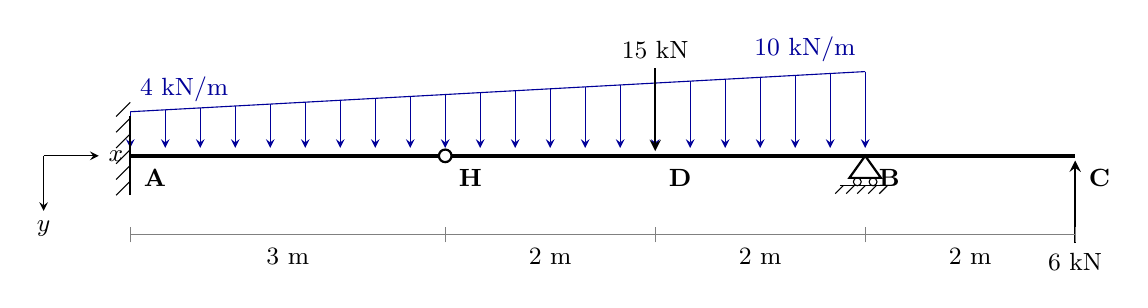
\begin{tikzpicture}
\draw[-stealth,blue!60!black] (0.0000,0.5600) -- (0.0000,0.1000);
\draw[-stealth,blue!60!black] (0.4444,0.5843) -- (0.4444,0.1000);
\draw[-stealth,blue!60!black] (0.8889,0.6086) -- (0.8889,0.1000);
\draw[-stealth,blue!60!black] (1.3333,0.6329) -- (1.3333,0.1000);
\draw[-stealth,blue!60!black] (1.7778,0.6571) -- (1.7778,0.1000);
\draw[-stealth,blue!60!black] (2.2222,0.6814) -- (2.2222,0.1000);
\draw[-stealth,blue!60!black] (2.6667,0.7057) -- (2.6667,0.1000);
\draw[-stealth,blue!60!black] (3.1111,0.7300) -- (3.1111,0.1000);
\draw[-stealth,blue!60!black] (3.5556,0.7543) -- (3.5556,0.1000);
\draw[-stealth,blue!60!black] (4.0000,0.7786) -- (4.0000,0.1000);
\draw[-stealth,blue!60!black] (4.4444,0.8029) -- (4.4444,0.1000);
\draw[-stealth,blue!60!black] (4.8889,0.8271) -- (4.8889,0.1000);
\draw[-stealth,blue!60!black] (5.3333,0.8514) -- (5.3333,0.1000);
\draw[-stealth,blue!60!black] (5.7778,0.8757) -- (5.7778,0.1000);
\draw[-stealth,blue!60!black] (6.2222,0.9000) -- (6.2222,0.1000);
\draw[-stealth,blue!60!black] (6.6667,0.9243) -- (6.6667,0.1000);
\draw[-stealth,blue!60!black] (7.1111,0.9486) -- (7.1111,0.1000);
\draw[-stealth,blue!60!black] (7.5556,0.9729) -- (7.5556,0.1000);
\draw[-stealth,blue!60!black] (8.0000,0.9971) -- (8.0000,0.1000);
\draw[-stealth,blue!60!black] (8.4444,1.0214) -- (8.4444,0.1000);
\draw[-stealth,blue!60!black] (8.8889,1.0457) -- (8.8889,0.1000);
\draw[-stealth,blue!60!black] (9.3333,1.0700) -- (9.3333,0.1000);
% studium:at distributed 0 x=0 to=7 check=span
\draw[blue!60!black] (0.0000,0.5600) -- (0.4444,0.5843) -- (0.8889,0.6086) -- (1.3333,0.6329) -- (1.7778,0.6571) -- (2.2222,0.6814) -- (2.6667,0.7057) -- (3.1111,0.7300) -- (3.5556,0.7543) -- (4.0000,0.7786) -- (4.4444,0.8029) -- (4.8889,0.8271) -- (5.3333,0.8514) -- (5.7778,0.8757) -- (6.2222,0.9000) -- (6.6667,0.9243) -- (7.1111,0.9486) -- (7.5556,0.9729) -- (8.0000,0.9971) -- (8.4444,1.0214) -- (8.8889,1.0457) -- (9.3333,1.0700);
\node[font=\small,anchor=south west,blue!60!black] at (0.0000,0.5600) {$4$~\mbox{kN/m}};
\node[font=\small,anchor=south east,blue!60!black] at (9.3333,1.0700) {$10$~\mbox{kN/m}};
\draw[line width=1.6pt] (0,0.0000) -- (12.0000,0.0000);
% studium:at support A x=0 check=first
\draw[thick] (0.0000,-0.5000) -- (0.0000,0.5000);
\draw (0.0000,-0.3200) -- (-0.1800,-0.5000);
\draw (0.0000,-0.1200) -- (-0.1800,-0.3000);
\draw (0.0000,0.0800) -- (-0.1800,-0.1000);
\draw (0.0000,0.2800) -- (-0.1800,0.1000);
\draw (0.0000,0.4800) -- (-0.1800,0.3000);
\draw (0.0000,0.6800) -- (-0.1800,0.5000);
% studium:at support B x=7 check=first
\draw[thick,fill=white] (9.3333,0.0000) -- (9.1333,-0.2800) -- (9.5333,-0.2800) -- cycle;
\draw (9.2333,-0.3300) circle (0.05);
\draw (9.4333,-0.3300) circle (0.05);
\draw (9.0133,-0.3800) -- (9.6533,-0.3800);
\draw (9.0533,-0.3800) -- (8.9533,-0.4800);
\draw (9.1933,-0.3800) -- (9.0933,-0.4800);
\draw (9.3333,-0.3800) -- (9.2333,-0.4800);
\draw (9.4733,-0.3800) -- (9.3733,-0.4800);
\draw (9.6133,-0.3800) -- (9.5133,-0.4800);
% studium:at hinge 0 x=3 check=first
\draw[thick,fill=white] (4.0000,0.0000) circle (0.08);
% studium:at force 0 x=5 check=tip
\draw[-stealth,thick,black] (6.6667,1.1100) -- (6.6667,0.0600);
\node[font=\small,anchor=south] at (6.6667,1.1100) {$15$~\mbox{kN}};
% studium:at force 1 x=9 check=tip
\draw[-stealth,thick,black] (12.0000,-1.1100) -- (12.0000,-0.0600);
\node[font=\small,anchor=north] at (12.0000,-1.1100) {$6$~\mbox{kN}};
\node[font=\small\bfseries,anchor=north west] at (0.0500,-0.0500) {A};
\node[font=\small\bfseries,anchor=north west] at (4.0500,-0.0500) {H};
\node[font=\small\bfseries,anchor=north west] at (6.7167,-0.0500) {D};
\node[font=\small\bfseries,anchor=north west] at (9.3833,-0.0500) {B};
\node[font=\small\bfseries,anchor=north west] at (12.0500,-0.0500) {C};
\draw[gray] (0,-1.0000) -- (12.0000,-1.0000);
\draw[gray] (0.0000,-1.1000) -- (0.0000,-0.9000);
\draw[gray] (4.0000,-1.1000) -- (4.0000,-0.9000);
\draw[gray] (6.6667,-1.1000) -- (6.6667,-0.9000);
\draw[gray] (9.3333,-1.1000) -- (9.3333,-0.9000);
\draw[gray] (12.0000,-1.1000) -- (12.0000,-0.9000);
\node[font=\small,anchor=north] at (2.0000,-1.0500) {$3$~\mbox{m}};
\node[font=\small,anchor=north] at (5.3333,-1.0500) {$2$~\mbox{m}};
\node[font=\small,anchor=north] at (8.0000,-1.0500) {$2$~\mbox{m}};
\node[font=\small,anchor=north] at (10.6667,-1.0500) {$2$~\mbox{m}};
\draw[-stealth] (-1.1,0.0000) -- (-0.4,0.0000) node[right,font=\small] {$x$};
\draw[-stealth] (-1.1,0.0000) -- (-1.1,-0.7000) node[below,font=\small] {$y$};
\end{tikzpicture}}%
\count0=\ht0
\advance\count0 by \dp0
\count2=\wd0
\count4=\dimexpr\textheight/100*38\relax
\count6=\linewidth
\ifnum\count0<1
\count0=1
\fi
\ifnum\count2<1
\count2=1
\fi
\divide\count0 by 4096
\divide\count2 by 4096
\divide\count4 by 4096
\divide\count6 by 4096
\ifnum\count0<1
\count0=1
\fi
\ifnum\count2<1
\count2=1
\fi
\ifnum\count4<1
\count4=1
\fi
\ifnum\count6<1
\count6=1
\fi
\count8=\count2
\ifnum\count0>\count4
\count8=\numexpr\count2*\count4/\count0\relax
\fi
\ifnum\count8>\count6
\resizebox{\linewidth}{!}{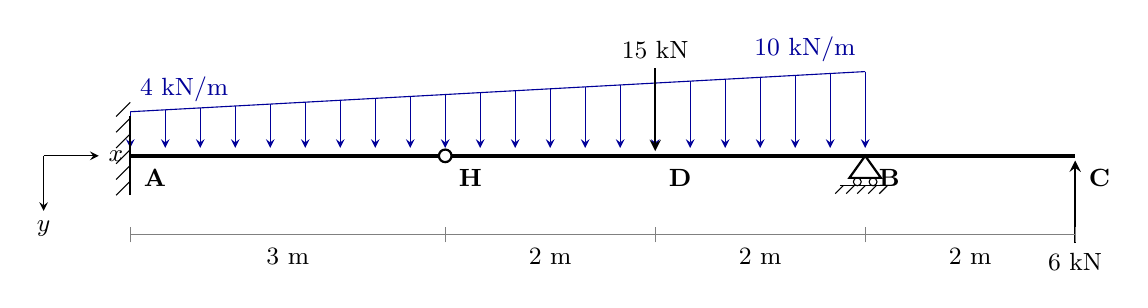
\begin{tikzpicture}
\draw[-stealth,blue!60!black] (0.0000,0.5600) -- (0.0000,0.1000);
\draw[-stealth,blue!60!black] (0.4444,0.5843) -- (0.4444,0.1000);
\draw[-stealth,blue!60!black] (0.8889,0.6086) -- (0.8889,0.1000);
\draw[-stealth,blue!60!black] (1.3333,0.6329) -- (1.3333,0.1000);
\draw[-stealth,blue!60!black] (1.7778,0.6571) -- (1.7778,0.1000);
\draw[-stealth,blue!60!black] (2.2222,0.6814) -- (2.2222,0.1000);
\draw[-stealth,blue!60!black] (2.6667,0.7057) -- (2.6667,0.1000);
\draw[-stealth,blue!60!black] (3.1111,0.7300) -- (3.1111,0.1000);
\draw[-stealth,blue!60!black] (3.5556,0.7543) -- (3.5556,0.1000);
\draw[-stealth,blue!60!black] (4.0000,0.7786) -- (4.0000,0.1000);
\draw[-stealth,blue!60!black] (4.4444,0.8029) -- (4.4444,0.1000);
\draw[-stealth,blue!60!black] (4.8889,0.8271) -- (4.8889,0.1000);
\draw[-stealth,blue!60!black] (5.3333,0.8514) -- (5.3333,0.1000);
\draw[-stealth,blue!60!black] (5.7778,0.8757) -- (5.7778,0.1000);
\draw[-stealth,blue!60!black] (6.2222,0.9000) -- (6.2222,0.1000);
\draw[-stealth,blue!60!black] (6.6667,0.9243) -- (6.6667,0.1000);
\draw[-stealth,blue!60!black] (7.1111,0.9486) -- (7.1111,0.1000);
\draw[-stealth,blue!60!black] (7.5556,0.9729) -- (7.5556,0.1000);
\draw[-stealth,blue!60!black] (8.0000,0.9971) -- (8.0000,0.1000);
\draw[-stealth,blue!60!black] (8.4444,1.0214) -- (8.4444,0.1000);
\draw[-stealth,blue!60!black] (8.8889,1.0457) -- (8.8889,0.1000);
\draw[-stealth,blue!60!black] (9.3333,1.0700) -- (9.3333,0.1000);
% studium:at distributed 0 x=0 to=7 check=span
\draw[blue!60!black] (0.0000,0.5600) -- (0.4444,0.5843) -- (0.8889,0.6086) -- (1.3333,0.6329) -- (1.7778,0.6571) -- (2.2222,0.6814) -- (2.6667,0.7057) -- (3.1111,0.7300) -- (3.5556,0.7543) -- (4.0000,0.7786) -- (4.4444,0.8029) -- (4.8889,0.8271) -- (5.3333,0.8514) -- (5.7778,0.8757) -- (6.2222,0.9000) -- (6.6667,0.9243) -- (7.1111,0.9486) -- (7.5556,0.9729) -- (8.0000,0.9971) -- (8.4444,1.0214) -- (8.8889,1.0457) -- (9.3333,1.0700);
\node[font=\small,anchor=south west,blue!60!black] at (0.0000,0.5600) {$4$~\mbox{kN/m}};
\node[font=\small,anchor=south east,blue!60!black] at (9.3333,1.0700) {$10$~\mbox{kN/m}};
\draw[line width=1.6pt] (0,0.0000) -- (12.0000,0.0000);
% studium:at support A x=0 check=first
\draw[thick] (0.0000,-0.5000) -- (0.0000,0.5000);
\draw (0.0000,-0.3200) -- (-0.1800,-0.5000);
\draw (0.0000,-0.1200) -- (-0.1800,-0.3000);
\draw (0.0000,0.0800) -- (-0.1800,-0.1000);
\draw (0.0000,0.2800) -- (-0.1800,0.1000);
\draw (0.0000,0.4800) -- (-0.1800,0.3000);
\draw (0.0000,0.6800) -- (-0.1800,0.5000);
% studium:at support B x=7 check=first
\draw[thick,fill=white] (9.3333,0.0000) -- (9.1333,-0.2800) -- (9.5333,-0.2800) -- cycle;
\draw (9.2333,-0.3300) circle (0.05);
\draw (9.4333,-0.3300) circle (0.05);
\draw (9.0133,-0.3800) -- (9.6533,-0.3800);
\draw (9.0533,-0.3800) -- (8.9533,-0.4800);
\draw (9.1933,-0.3800) -- (9.0933,-0.4800);
\draw (9.3333,-0.3800) -- (9.2333,-0.4800);
\draw (9.4733,-0.3800) -- (9.3733,-0.4800);
\draw (9.6133,-0.3800) -- (9.5133,-0.4800);
% studium:at hinge 0 x=3 check=first
\draw[thick,fill=white] (4.0000,0.0000) circle (0.08);
% studium:at force 0 x=5 check=tip
\draw[-stealth,thick,black] (6.6667,1.1100) -- (6.6667,0.0600);
\node[font=\small,anchor=south] at (6.6667,1.1100) {$15$~\mbox{kN}};
% studium:at force 1 x=9 check=tip
\draw[-stealth,thick,black] (12.0000,-1.1100) -- (12.0000,-0.0600);
\node[font=\small,anchor=north] at (12.0000,-1.1100) {$6$~\mbox{kN}};
\node[font=\small\bfseries,anchor=north west] at (0.0500,-0.0500) {A};
\node[font=\small\bfseries,anchor=north west] at (4.0500,-0.0500) {H};
\node[font=\small\bfseries,anchor=north west] at (6.7167,-0.0500) {D};
\node[font=\small\bfseries,anchor=north west] at (9.3833,-0.0500) {B};
\node[font=\small\bfseries,anchor=north west] at (12.0500,-0.0500) {C};
\draw[gray] (0,-1.0000) -- (12.0000,-1.0000);
\draw[gray] (0.0000,-1.1000) -- (0.0000,-0.9000);
\draw[gray] (4.0000,-1.1000) -- (4.0000,-0.9000);
\draw[gray] (6.6667,-1.1000) -- (6.6667,-0.9000);
\draw[gray] (9.3333,-1.1000) -- (9.3333,-0.9000);
\draw[gray] (12.0000,-1.1000) -- (12.0000,-0.9000);
\node[font=\small,anchor=north] at (2.0000,-1.0500) {$3$~\mbox{m}};
\node[font=\small,anchor=north] at (5.3333,-1.0500) {$2$~\mbox{m}};
\node[font=\small,anchor=north] at (8.0000,-1.0500) {$2$~\mbox{m}};
\node[font=\small,anchor=north] at (10.6667,-1.0500) {$2$~\mbox{m}};
\draw[-stealth] (-1.1,0.0000) -- (-0.4,0.0000) node[right,font=\small] {$x$};
\draw[-stealth] (-1.1,0.0000) -- (-1.1,-0.7000) node[below,font=\small] {$y$};
\end{tikzpicture}}%
\else
\ifnum\count0>\count4
\resizebox{!}{\dimexpr\textheight/100*38\relax}{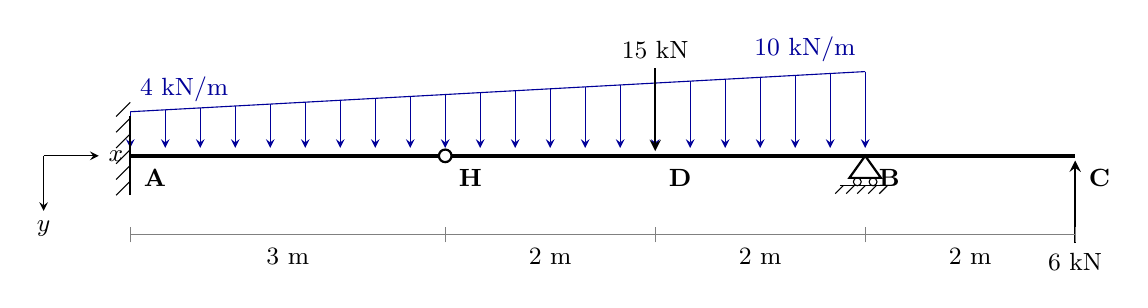
\begin{tikzpicture}
\draw[-stealth,blue!60!black] (0.0000,0.5600) -- (0.0000,0.1000);
\draw[-stealth,blue!60!black] (0.4444,0.5843) -- (0.4444,0.1000);
\draw[-stealth,blue!60!black] (0.8889,0.6086) -- (0.8889,0.1000);
\draw[-stealth,blue!60!black] (1.3333,0.6329) -- (1.3333,0.1000);
\draw[-stealth,blue!60!black] (1.7778,0.6571) -- (1.7778,0.1000);
\draw[-stealth,blue!60!black] (2.2222,0.6814) -- (2.2222,0.1000);
\draw[-stealth,blue!60!black] (2.6667,0.7057) -- (2.6667,0.1000);
\draw[-stealth,blue!60!black] (3.1111,0.7300) -- (3.1111,0.1000);
\draw[-stealth,blue!60!black] (3.5556,0.7543) -- (3.5556,0.1000);
\draw[-stealth,blue!60!black] (4.0000,0.7786) -- (4.0000,0.1000);
\draw[-stealth,blue!60!black] (4.4444,0.8029) -- (4.4444,0.1000);
\draw[-stealth,blue!60!black] (4.8889,0.8271) -- (4.8889,0.1000);
\draw[-stealth,blue!60!black] (5.3333,0.8514) -- (5.3333,0.1000);
\draw[-stealth,blue!60!black] (5.7778,0.8757) -- (5.7778,0.1000);
\draw[-stealth,blue!60!black] (6.2222,0.9000) -- (6.2222,0.1000);
\draw[-stealth,blue!60!black] (6.6667,0.9243) -- (6.6667,0.1000);
\draw[-stealth,blue!60!black] (7.1111,0.9486) -- (7.1111,0.1000);
\draw[-stealth,blue!60!black] (7.5556,0.9729) -- (7.5556,0.1000);
\draw[-stealth,blue!60!black] (8.0000,0.9971) -- (8.0000,0.1000);
\draw[-stealth,blue!60!black] (8.4444,1.0214) -- (8.4444,0.1000);
\draw[-stealth,blue!60!black] (8.8889,1.0457) -- (8.8889,0.1000);
\draw[-stealth,blue!60!black] (9.3333,1.0700) -- (9.3333,0.1000);
% studium:at distributed 0 x=0 to=7 check=span
\draw[blue!60!black] (0.0000,0.5600) -- (0.4444,0.5843) -- (0.8889,0.6086) -- (1.3333,0.6329) -- (1.7778,0.6571) -- (2.2222,0.6814) -- (2.6667,0.7057) -- (3.1111,0.7300) -- (3.5556,0.7543) -- (4.0000,0.7786) -- (4.4444,0.8029) -- (4.8889,0.8271) -- (5.3333,0.8514) -- (5.7778,0.8757) -- (6.2222,0.9000) -- (6.6667,0.9243) -- (7.1111,0.9486) -- (7.5556,0.9729) -- (8.0000,0.9971) -- (8.4444,1.0214) -- (8.8889,1.0457) -- (9.3333,1.0700);
\node[font=\small,anchor=south west,blue!60!black] at (0.0000,0.5600) {$4$~\mbox{kN/m}};
\node[font=\small,anchor=south east,blue!60!black] at (9.3333,1.0700) {$10$~\mbox{kN/m}};
\draw[line width=1.6pt] (0,0.0000) -- (12.0000,0.0000);
% studium:at support A x=0 check=first
\draw[thick] (0.0000,-0.5000) -- (0.0000,0.5000);
\draw (0.0000,-0.3200) -- (-0.1800,-0.5000);
\draw (0.0000,-0.1200) -- (-0.1800,-0.3000);
\draw (0.0000,0.0800) -- (-0.1800,-0.1000);
\draw (0.0000,0.2800) -- (-0.1800,0.1000);
\draw (0.0000,0.4800) -- (-0.1800,0.3000);
\draw (0.0000,0.6800) -- (-0.1800,0.5000);
% studium:at support B x=7 check=first
\draw[thick,fill=white] (9.3333,0.0000) -- (9.1333,-0.2800) -- (9.5333,-0.2800) -- cycle;
\draw (9.2333,-0.3300) circle (0.05);
\draw (9.4333,-0.3300) circle (0.05);
\draw (9.0133,-0.3800) -- (9.6533,-0.3800);
\draw (9.0533,-0.3800) -- (8.9533,-0.4800);
\draw (9.1933,-0.3800) -- (9.0933,-0.4800);
\draw (9.3333,-0.3800) -- (9.2333,-0.4800);
\draw (9.4733,-0.3800) -- (9.3733,-0.4800);
\draw (9.6133,-0.3800) -- (9.5133,-0.4800);
% studium:at hinge 0 x=3 check=first
\draw[thick,fill=white] (4.0000,0.0000) circle (0.08);
% studium:at force 0 x=5 check=tip
\draw[-stealth,thick,black] (6.6667,1.1100) -- (6.6667,0.0600);
\node[font=\small,anchor=south] at (6.6667,1.1100) {$15$~\mbox{kN}};
% studium:at force 1 x=9 check=tip
\draw[-stealth,thick,black] (12.0000,-1.1100) -- (12.0000,-0.0600);
\node[font=\small,anchor=north] at (12.0000,-1.1100) {$6$~\mbox{kN}};
\node[font=\small\bfseries,anchor=north west] at (0.0500,-0.0500) {A};
\node[font=\small\bfseries,anchor=north west] at (4.0500,-0.0500) {H};
\node[font=\small\bfseries,anchor=north west] at (6.7167,-0.0500) {D};
\node[font=\small\bfseries,anchor=north west] at (9.3833,-0.0500) {B};
\node[font=\small\bfseries,anchor=north west] at (12.0500,-0.0500) {C};
\draw[gray] (0,-1.0000) -- (12.0000,-1.0000);
\draw[gray] (0.0000,-1.1000) -- (0.0000,-0.9000);
\draw[gray] (4.0000,-1.1000) -- (4.0000,-0.9000);
\draw[gray] (6.6667,-1.1000) -- (6.6667,-0.9000);
\draw[gray] (9.3333,-1.1000) -- (9.3333,-0.9000);
\draw[gray] (12.0000,-1.1000) -- (12.0000,-0.9000);
\node[font=\small,anchor=north] at (2.0000,-1.0500) {$3$~\mbox{m}};
\node[font=\small,anchor=north] at (5.3333,-1.0500) {$2$~\mbox{m}};
\node[font=\small,anchor=north] at (8.0000,-1.0500) {$2$~\mbox{m}};
\node[font=\small,anchor=north] at (10.6667,-1.0500) {$2$~\mbox{m}};
\draw[-stealth] (-1.1,0.0000) -- (-0.4,0.0000) node[right,font=\small] {$x$};
\draw[-stealth] (-1.1,0.0000) -- (-1.1,-0.7000) node[below,font=\small] {$y$};
\end{tikzpicture}}%
\else
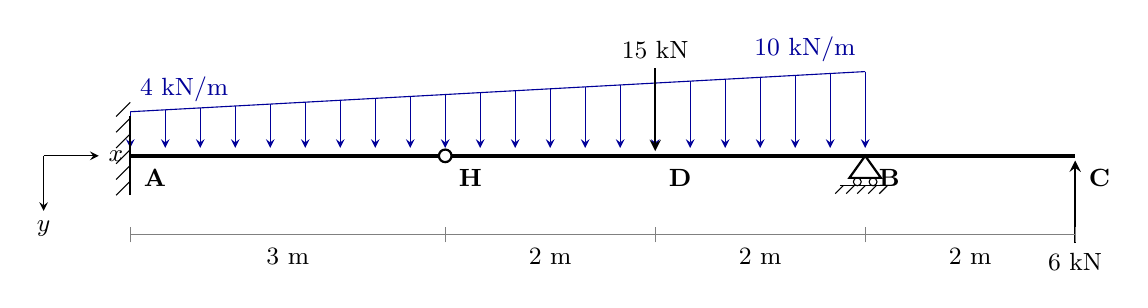
\begin{tikzpicture}
\draw[-stealth,blue!60!black] (0.0000,0.5600) -- (0.0000,0.1000);
\draw[-stealth,blue!60!black] (0.4444,0.5843) -- (0.4444,0.1000);
\draw[-stealth,blue!60!black] (0.8889,0.6086) -- (0.8889,0.1000);
\draw[-stealth,blue!60!black] (1.3333,0.6329) -- (1.3333,0.1000);
\draw[-stealth,blue!60!black] (1.7778,0.6571) -- (1.7778,0.1000);
\draw[-stealth,blue!60!black] (2.2222,0.6814) -- (2.2222,0.1000);
\draw[-stealth,blue!60!black] (2.6667,0.7057) -- (2.6667,0.1000);
\draw[-stealth,blue!60!black] (3.1111,0.7300) -- (3.1111,0.1000);
\draw[-stealth,blue!60!black] (3.5556,0.7543) -- (3.5556,0.1000);
\draw[-stealth,blue!60!black] (4.0000,0.7786) -- (4.0000,0.1000);
\draw[-stealth,blue!60!black] (4.4444,0.8029) -- (4.4444,0.1000);
\draw[-stealth,blue!60!black] (4.8889,0.8271) -- (4.8889,0.1000);
\draw[-stealth,blue!60!black] (5.3333,0.8514) -- (5.3333,0.1000);
\draw[-stealth,blue!60!black] (5.7778,0.8757) -- (5.7778,0.1000);
\draw[-stealth,blue!60!black] (6.2222,0.9000) -- (6.2222,0.1000);
\draw[-stealth,blue!60!black] (6.6667,0.9243) -- (6.6667,0.1000);
\draw[-stealth,blue!60!black] (7.1111,0.9486) -- (7.1111,0.1000);
\draw[-stealth,blue!60!black] (7.5556,0.9729) -- (7.5556,0.1000);
\draw[-stealth,blue!60!black] (8.0000,0.9971) -- (8.0000,0.1000);
\draw[-stealth,blue!60!black] (8.4444,1.0214) -- (8.4444,0.1000);
\draw[-stealth,blue!60!black] (8.8889,1.0457) -- (8.8889,0.1000);
\draw[-stealth,blue!60!black] (9.3333,1.0700) -- (9.3333,0.1000);
% studium:at distributed 0 x=0 to=7 check=span
\draw[blue!60!black] (0.0000,0.5600) -- (0.4444,0.5843) -- (0.8889,0.6086) -- (1.3333,0.6329) -- (1.7778,0.6571) -- (2.2222,0.6814) -- (2.6667,0.7057) -- (3.1111,0.7300) -- (3.5556,0.7543) -- (4.0000,0.7786) -- (4.4444,0.8029) -- (4.8889,0.8271) -- (5.3333,0.8514) -- (5.7778,0.8757) -- (6.2222,0.9000) -- (6.6667,0.9243) -- (7.1111,0.9486) -- (7.5556,0.9729) -- (8.0000,0.9971) -- (8.4444,1.0214) -- (8.8889,1.0457) -- (9.3333,1.0700);
\node[font=\small,anchor=south west,blue!60!black] at (0.0000,0.5600) {$4$~\mbox{kN/m}};
\node[font=\small,anchor=south east,blue!60!black] at (9.3333,1.0700) {$10$~\mbox{kN/m}};
\draw[line width=1.6pt] (0,0.0000) -- (12.0000,0.0000);
% studium:at support A x=0 check=first
\draw[thick] (0.0000,-0.5000) -- (0.0000,0.5000);
\draw (0.0000,-0.3200) -- (-0.1800,-0.5000);
\draw (0.0000,-0.1200) -- (-0.1800,-0.3000);
\draw (0.0000,0.0800) -- (-0.1800,-0.1000);
\draw (0.0000,0.2800) -- (-0.1800,0.1000);
\draw (0.0000,0.4800) -- (-0.1800,0.3000);
\draw (0.0000,0.6800) -- (-0.1800,0.5000);
% studium:at support B x=7 check=first
\draw[thick,fill=white] (9.3333,0.0000) -- (9.1333,-0.2800) -- (9.5333,-0.2800) -- cycle;
\draw (9.2333,-0.3300) circle (0.05);
\draw (9.4333,-0.3300) circle (0.05);
\draw (9.0133,-0.3800) -- (9.6533,-0.3800);
\draw (9.0533,-0.3800) -- (8.9533,-0.4800);
\draw (9.1933,-0.3800) -- (9.0933,-0.4800);
\draw (9.3333,-0.3800) -- (9.2333,-0.4800);
\draw (9.4733,-0.3800) -- (9.3733,-0.4800);
\draw (9.6133,-0.3800) -- (9.5133,-0.4800);
% studium:at hinge 0 x=3 check=first
\draw[thick,fill=white] (4.0000,0.0000) circle (0.08);
% studium:at force 0 x=5 check=tip
\draw[-stealth,thick,black] (6.6667,1.1100) -- (6.6667,0.0600);
\node[font=\small,anchor=south] at (6.6667,1.1100) {$15$~\mbox{kN}};
% studium:at force 1 x=9 check=tip
\draw[-stealth,thick,black] (12.0000,-1.1100) -- (12.0000,-0.0600);
\node[font=\small,anchor=north] at (12.0000,-1.1100) {$6$~\mbox{kN}};
\node[font=\small\bfseries,anchor=north west] at (0.0500,-0.0500) {A};
\node[font=\small\bfseries,anchor=north west] at (4.0500,-0.0500) {H};
\node[font=\small\bfseries,anchor=north west] at (6.7167,-0.0500) {D};
\node[font=\small\bfseries,anchor=north west] at (9.3833,-0.0500) {B};
\node[font=\small\bfseries,anchor=north west] at (12.0500,-0.0500) {C};
\draw[gray] (0,-1.0000) -- (12.0000,-1.0000);
\draw[gray] (0.0000,-1.1000) -- (0.0000,-0.9000);
\draw[gray] (4.0000,-1.1000) -- (4.0000,-0.9000);
\draw[gray] (6.6667,-1.1000) -- (6.6667,-0.9000);
\draw[gray] (9.3333,-1.1000) -- (9.3333,-0.9000);
\draw[gray] (12.0000,-1.1000) -- (12.0000,-0.9000);
\node[font=\small,anchor=north] at (2.0000,-1.0500) {$3$~\mbox{m}};
\node[font=\small,anchor=north] at (5.3333,-1.0500) {$2$~\mbox{m}};
\node[font=\small,anchor=north] at (8.0000,-1.0500) {$2$~\mbox{m}};
\node[font=\small,anchor=north] at (10.6667,-1.0500) {$2$~\mbox{m}};
\draw[-stealth] (-1.1,0.0000) -- (-0.4,0.0000) node[right,font=\small] {$x$};
\draw[-stealth] (-1.1,0.0000) -- (-1.1,-0.7000) node[below,font=\small] {$y$};
\end{tikzpicture}%
\fi
\fi
\endgroup
\par\nopagebreak
\studiumcaption{fig:e2-c03-gerber-enunciado}{Viga con empotramiento, rótula \(H\), apoyo móvil \(B\) y voladizo, con carga trapezoidal y cargas puntuales.}
\end{minipage}\par\medskip

\textbf{Hipótesis.}\begin{itemize}\item viga plana con cargas verticales, sin axil
\item la rótula transmite cortante pero no flector
\item criterio de signos del curso\end{itemize}

\textbf{Modelo y desarrollo.}

Flector nulo en la rótula (parte derecha).\[\fitmath{R_B\,(x_B - x_H) + F\,(x_C - x_H) = \int_{x_H}^{x_B} q(t)\,(t - x_H)\,\mathrm{d}t + P\,(x_D - x_H)}\]

\textbf{Procedimiento.}\begin{itemize}\item Las incógnitas son $R_A$, $M_A$ y $R_B$, y hay tres ecuaciones: equilibrio vertical, momentos y flector nulo en $H$. La rótula hace isostática una viga que sin ella sería hiperestática.
\item La parte $HC$ solo contiene $R_B$ como incógnita, así que el flector nulo en $H$, escrito con la parte derecha, da $R_B$ directamente.
\item Con $R_B$ conocida, el equilibrio vertical da $R_A$ y el de momentos respecto a $A$ da el momento del empotramiento.
\item Los tramos son $AH$, $HD$, $DB$ y $BC$. En $AH$ y $HD$ la ley es la misma, porque en la rótula no actúa ninguna carga; el cortante salta en $D$ y en $B$.
\item El cortante del tramo $DB$ no se anula, de modo que el flector máximo positivo está en $D$, donde el cortante cambia de signo; el mínimo está en el empotramiento.\end{itemize}

\textbf{Cálculo de los pasos.}

\begin{enumerate}

\item Momento de la carga de HB respecto a H.

\[\fitmath{y_{1}=\frac{\frac{46}{7}\cdot {4}^{2}}{2}+\frac{\frac{6}{7}\cdot {4}^{3}}{3}\approx 70.85714\,\mathrm{kN m}}\]

\item Reacción en B (flector nulo en H).

\[\fitmath{y_{2}=\frac{\frac{496}{7}+15\cdot 2-6\cdot 6}{4}\approx 16.21429\,\mathrm{kN}}\]

\item Reacción en A.

\[\fitmath{y_{3}=\frac{4+10}{2}\cdot 7+15-6-\frac{\frac{496}{7}+15\cdot 2-6\cdot 6}{4}\approx 41.78571\,\mathrm{kN}}\]

\item Flector en el empotramiento, con la parte derecha.

\[\fitmath{y_{4}=\frac{\frac{496}{7}+15\cdot 2-6\cdot 6}{4}\cdot 7+6\cdot 9-\left(\frac{4\cdot {7}^{2}}{2}+\frac{\frac{6}{7}\cdot {7}^{3}}{3}\right)-15\cdot 5\approx -103.5\,\mathrm{kN m}}\]

\end{enumerate}

\par\medskip\noindent\begin{minipage}{\linewidth}
\centering
\begingroup
\setbox0=\hbox{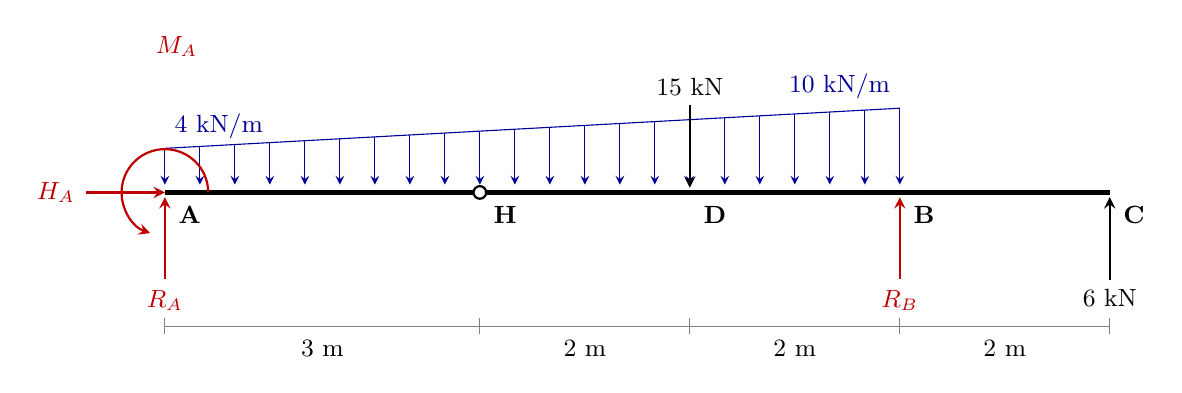
\begin{tikzpicture}
\draw[-stealth,blue!60!black] (0.0000,0.5600) -- (0.0000,0.1000);
\draw[-stealth,blue!60!black] (0.4444,0.5843) -- (0.4444,0.1000);
\draw[-stealth,blue!60!black] (0.8889,0.6086) -- (0.8889,0.1000);
\draw[-stealth,blue!60!black] (1.3333,0.6329) -- (1.3333,0.1000);
\draw[-stealth,blue!60!black] (1.7778,0.6571) -- (1.7778,0.1000);
\draw[-stealth,blue!60!black] (2.2222,0.6814) -- (2.2222,0.1000);
\draw[-stealth,blue!60!black] (2.6667,0.7057) -- (2.6667,0.1000);
\draw[-stealth,blue!60!black] (3.1111,0.7300) -- (3.1111,0.1000);
\draw[-stealth,blue!60!black] (3.5556,0.7543) -- (3.5556,0.1000);
\draw[-stealth,blue!60!black] (4.0000,0.7786) -- (4.0000,0.1000);
\draw[-stealth,blue!60!black] (4.4444,0.8029) -- (4.4444,0.1000);
\draw[-stealth,blue!60!black] (4.8889,0.8271) -- (4.8889,0.1000);
\draw[-stealth,blue!60!black] (5.3333,0.8514) -- (5.3333,0.1000);
\draw[-stealth,blue!60!black] (5.7778,0.8757) -- (5.7778,0.1000);
\draw[-stealth,blue!60!black] (6.2222,0.9000) -- (6.2222,0.1000);
\draw[-stealth,blue!60!black] (6.6667,0.9243) -- (6.6667,0.1000);
\draw[-stealth,blue!60!black] (7.1111,0.9486) -- (7.1111,0.1000);
\draw[-stealth,blue!60!black] (7.5556,0.9729) -- (7.5556,0.1000);
\draw[-stealth,blue!60!black] (8.0000,0.9971) -- (8.0000,0.1000);
\draw[-stealth,blue!60!black] (8.4444,1.0214) -- (8.4444,0.1000);
\draw[-stealth,blue!60!black] (8.8889,1.0457) -- (8.8889,0.1000);
\draw[-stealth,blue!60!black] (9.3333,1.0700) -- (9.3333,0.1000);
% studium:at distributed 0 x=0 to=7 check=span
\draw[blue!60!black] (0.0000,0.5600) -- (0.4444,0.5843) -- (0.8889,0.6086) -- (1.3333,0.6329) -- (1.7778,0.6571) -- (2.2222,0.6814) -- (2.6667,0.7057) -- (3.1111,0.7300) -- (3.5556,0.7543) -- (4.0000,0.7786) -- (4.4444,0.8029) -- (4.8889,0.8271) -- (5.3333,0.8514) -- (5.7778,0.8757) -- (6.2222,0.9000) -- (6.6667,0.9243) -- (7.1111,0.9486) -- (7.5556,0.9729) -- (8.0000,0.9971) -- (8.4444,1.0214) -- (8.8889,1.0457) -- (9.3333,1.0700);
\node[font=\small,anchor=south west,blue!60!black] at (0.0000,0.5600) {$4$~\mbox{kN/m}};
\node[font=\small,anchor=south east,blue!60!black] at (9.3333,1.0700) {$10$~\mbox{kN/m}};
\draw[line width=1.6pt] (0,0.0000) -- (12.0000,0.0000);
% studium:at hinge 0 x=3 check=first
\draw[thick,fill=white] (4.0000,0.0000) circle (0.08);
% studium:at force 0 x=5 check=tip
\draw[-stealth,thick,black] (6.6667,1.1100) -- (6.6667,0.0600);
\node[font=\small,anchor=south] at (6.6667,1.1100) {$15$~\mbox{kN}};
% studium:at force 1 x=9 check=tip
\draw[-stealth,thick,black] (12.0000,-1.1100) -- (12.0000,-0.0600);
\node[font=\small,anchor=north] at (12.0000,-1.1100) {$6$~\mbox{kN}};
% studium:at reaction H_A x=0 check=tip
\draw[-stealth,thick,red!75!black] (-1.0000,0.0000) -- (0.0000,0.0000);
\node[font=\small,anchor=east,red!75!black] at (-1.0200,0.0000) {$H_{A}$};
% studium:at reaction R_A x=0 check=tip
\draw[-stealth,thick,red!75!black] (0.0000,-1.1000) -- (0.0000,-0.0600);
\node[font=\small,anchor=north,red!75!black] at (0.0000,-1.1200) {$R_{A}$};
% studium:at reaction M_A x=0 check=arc
\draw[-stealth,thick,red!75!black] (0.5500,0.0000) arc (0:250:0.55);
\node[font=\small,anchor=south,red!75!black] at (0.1500,1.6000) {$M_{A}$};
% studium:at reaction R_B x=7 check=tip
\draw[-stealth,thick,red!75!black] (9.3333,-1.1000) -- (9.3333,-0.0600);
\node[font=\small,anchor=north,red!75!black] at (9.3333,-1.1200) {$R_{B}$};
\node[font=\small\bfseries,anchor=north west] at (0.0500,-0.0500) {A};
\node[font=\small\bfseries,anchor=north west] at (4.0500,-0.0500) {H};
\node[font=\small\bfseries,anchor=north west] at (6.7167,-0.0500) {D};
\node[font=\small\bfseries,anchor=north west] at (9.3833,-0.0500) {B};
\node[font=\small\bfseries,anchor=north west] at (12.0500,-0.0500) {C};
\draw[gray] (0,-1.7000) -- (12.0000,-1.7000);
\draw[gray] (0.0000,-1.8000) -- (0.0000,-1.6000);
\draw[gray] (4.0000,-1.8000) -- (4.0000,-1.6000);
\draw[gray] (6.6667,-1.8000) -- (6.6667,-1.6000);
\draw[gray] (9.3333,-1.8000) -- (9.3333,-1.6000);
\draw[gray] (12.0000,-1.8000) -- (12.0000,-1.6000);
\node[font=\small,anchor=north] at (2.0000,-1.7500) {$3$~\mbox{m}};
\node[font=\small,anchor=north] at (5.3333,-1.7500) {$2$~\mbox{m}};
\node[font=\small,anchor=north] at (8.0000,-1.7500) {$2$~\mbox{m}};
\node[font=\small,anchor=north] at (10.6667,-1.7500) {$2$~\mbox{m}};
\end{tikzpicture}}%
\count0=\ht0
\advance\count0 by \dp0
\count2=\wd0
\count4=\dimexpr\textheight/100*38\relax
\count6=\linewidth
\ifnum\count0<1
\count0=1
\fi
\ifnum\count2<1
\count2=1
\fi
\divide\count0 by 4096
\divide\count2 by 4096
\divide\count4 by 4096
\divide\count6 by 4096
\ifnum\count0<1
\count0=1
\fi
\ifnum\count2<1
\count2=1
\fi
\ifnum\count4<1
\count4=1
\fi
\ifnum\count6<1
\count6=1
\fi
\count8=\count2
\ifnum\count0>\count4
\count8=\numexpr\count2*\count4/\count0\relax
\fi
\ifnum\count8>\count6
\resizebox{\linewidth}{!}{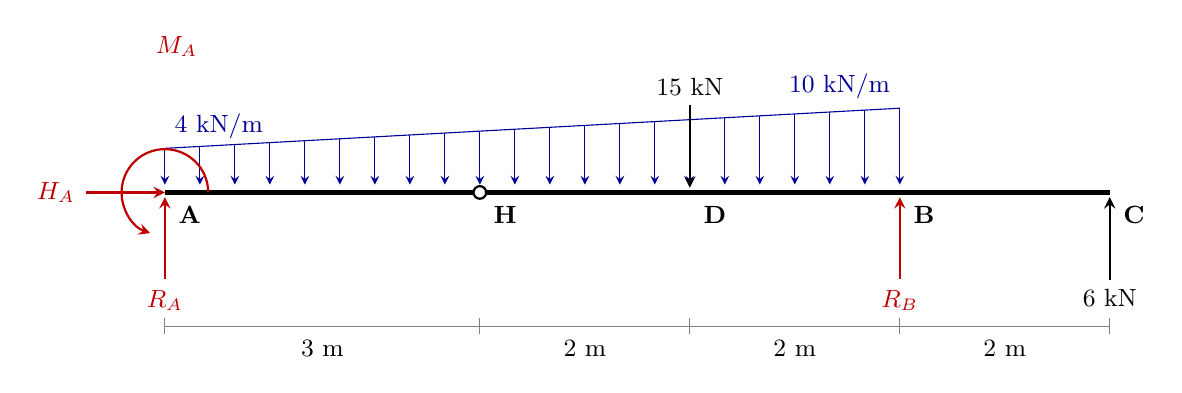
\begin{tikzpicture}
\draw[-stealth,blue!60!black] (0.0000,0.5600) -- (0.0000,0.1000);
\draw[-stealth,blue!60!black] (0.4444,0.5843) -- (0.4444,0.1000);
\draw[-stealth,blue!60!black] (0.8889,0.6086) -- (0.8889,0.1000);
\draw[-stealth,blue!60!black] (1.3333,0.6329) -- (1.3333,0.1000);
\draw[-stealth,blue!60!black] (1.7778,0.6571) -- (1.7778,0.1000);
\draw[-stealth,blue!60!black] (2.2222,0.6814) -- (2.2222,0.1000);
\draw[-stealth,blue!60!black] (2.6667,0.7057) -- (2.6667,0.1000);
\draw[-stealth,blue!60!black] (3.1111,0.7300) -- (3.1111,0.1000);
\draw[-stealth,blue!60!black] (3.5556,0.7543) -- (3.5556,0.1000);
\draw[-stealth,blue!60!black] (4.0000,0.7786) -- (4.0000,0.1000);
\draw[-stealth,blue!60!black] (4.4444,0.8029) -- (4.4444,0.1000);
\draw[-stealth,blue!60!black] (4.8889,0.8271) -- (4.8889,0.1000);
\draw[-stealth,blue!60!black] (5.3333,0.8514) -- (5.3333,0.1000);
\draw[-stealth,blue!60!black] (5.7778,0.8757) -- (5.7778,0.1000);
\draw[-stealth,blue!60!black] (6.2222,0.9000) -- (6.2222,0.1000);
\draw[-stealth,blue!60!black] (6.6667,0.9243) -- (6.6667,0.1000);
\draw[-stealth,blue!60!black] (7.1111,0.9486) -- (7.1111,0.1000);
\draw[-stealth,blue!60!black] (7.5556,0.9729) -- (7.5556,0.1000);
\draw[-stealth,blue!60!black] (8.0000,0.9971) -- (8.0000,0.1000);
\draw[-stealth,blue!60!black] (8.4444,1.0214) -- (8.4444,0.1000);
\draw[-stealth,blue!60!black] (8.8889,1.0457) -- (8.8889,0.1000);
\draw[-stealth,blue!60!black] (9.3333,1.0700) -- (9.3333,0.1000);
% studium:at distributed 0 x=0 to=7 check=span
\draw[blue!60!black] (0.0000,0.5600) -- (0.4444,0.5843) -- (0.8889,0.6086) -- (1.3333,0.6329) -- (1.7778,0.6571) -- (2.2222,0.6814) -- (2.6667,0.7057) -- (3.1111,0.7300) -- (3.5556,0.7543) -- (4.0000,0.7786) -- (4.4444,0.8029) -- (4.8889,0.8271) -- (5.3333,0.8514) -- (5.7778,0.8757) -- (6.2222,0.9000) -- (6.6667,0.9243) -- (7.1111,0.9486) -- (7.5556,0.9729) -- (8.0000,0.9971) -- (8.4444,1.0214) -- (8.8889,1.0457) -- (9.3333,1.0700);
\node[font=\small,anchor=south west,blue!60!black] at (0.0000,0.5600) {$4$~\mbox{kN/m}};
\node[font=\small,anchor=south east,blue!60!black] at (9.3333,1.0700) {$10$~\mbox{kN/m}};
\draw[line width=1.6pt] (0,0.0000) -- (12.0000,0.0000);
% studium:at hinge 0 x=3 check=first
\draw[thick,fill=white] (4.0000,0.0000) circle (0.08);
% studium:at force 0 x=5 check=tip
\draw[-stealth,thick,black] (6.6667,1.1100) -- (6.6667,0.0600);
\node[font=\small,anchor=south] at (6.6667,1.1100) {$15$~\mbox{kN}};
% studium:at force 1 x=9 check=tip
\draw[-stealth,thick,black] (12.0000,-1.1100) -- (12.0000,-0.0600);
\node[font=\small,anchor=north] at (12.0000,-1.1100) {$6$~\mbox{kN}};
% studium:at reaction H_A x=0 check=tip
\draw[-stealth,thick,red!75!black] (-1.0000,0.0000) -- (0.0000,0.0000);
\node[font=\small,anchor=east,red!75!black] at (-1.0200,0.0000) {$H_{A}$};
% studium:at reaction R_A x=0 check=tip
\draw[-stealth,thick,red!75!black] (0.0000,-1.1000) -- (0.0000,-0.0600);
\node[font=\small,anchor=north,red!75!black] at (0.0000,-1.1200) {$R_{A}$};
% studium:at reaction M_A x=0 check=arc
\draw[-stealth,thick,red!75!black] (0.5500,0.0000) arc (0:250:0.55);
\node[font=\small,anchor=south,red!75!black] at (0.1500,1.6000) {$M_{A}$};
% studium:at reaction R_B x=7 check=tip
\draw[-stealth,thick,red!75!black] (9.3333,-1.1000) -- (9.3333,-0.0600);
\node[font=\small,anchor=north,red!75!black] at (9.3333,-1.1200) {$R_{B}$};
\node[font=\small\bfseries,anchor=north west] at (0.0500,-0.0500) {A};
\node[font=\small\bfseries,anchor=north west] at (4.0500,-0.0500) {H};
\node[font=\small\bfseries,anchor=north west] at (6.7167,-0.0500) {D};
\node[font=\small\bfseries,anchor=north west] at (9.3833,-0.0500) {B};
\node[font=\small\bfseries,anchor=north west] at (12.0500,-0.0500) {C};
\draw[gray] (0,-1.7000) -- (12.0000,-1.7000);
\draw[gray] (0.0000,-1.8000) -- (0.0000,-1.6000);
\draw[gray] (4.0000,-1.8000) -- (4.0000,-1.6000);
\draw[gray] (6.6667,-1.8000) -- (6.6667,-1.6000);
\draw[gray] (9.3333,-1.8000) -- (9.3333,-1.6000);
\draw[gray] (12.0000,-1.8000) -- (12.0000,-1.6000);
\node[font=\small,anchor=north] at (2.0000,-1.7500) {$3$~\mbox{m}};
\node[font=\small,anchor=north] at (5.3333,-1.7500) {$2$~\mbox{m}};
\node[font=\small,anchor=north] at (8.0000,-1.7500) {$2$~\mbox{m}};
\node[font=\small,anchor=north] at (10.6667,-1.7500) {$2$~\mbox{m}};
\end{tikzpicture}}%
\else
\ifnum\count0>\count4
\resizebox{!}{\dimexpr\textheight/100*38\relax}{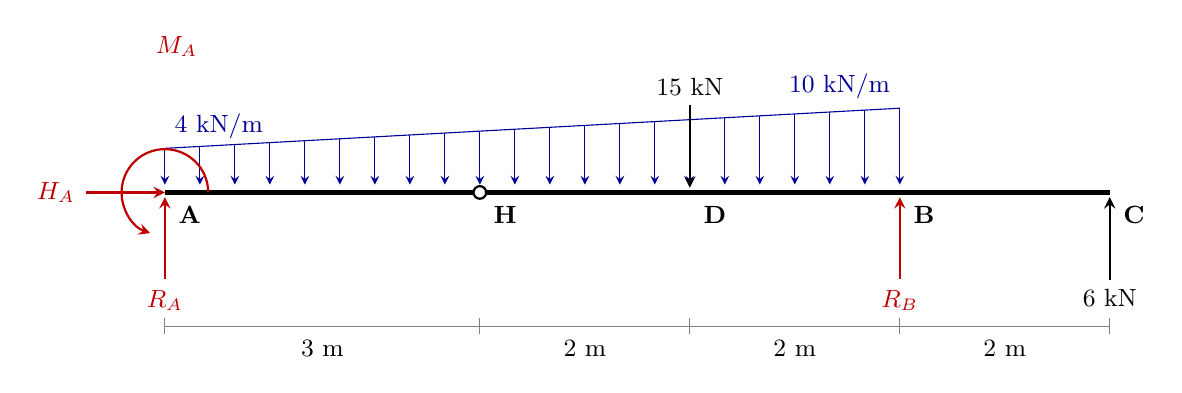
\begin{tikzpicture}
\draw[-stealth,blue!60!black] (0.0000,0.5600) -- (0.0000,0.1000);
\draw[-stealth,blue!60!black] (0.4444,0.5843) -- (0.4444,0.1000);
\draw[-stealth,blue!60!black] (0.8889,0.6086) -- (0.8889,0.1000);
\draw[-stealth,blue!60!black] (1.3333,0.6329) -- (1.3333,0.1000);
\draw[-stealth,blue!60!black] (1.7778,0.6571) -- (1.7778,0.1000);
\draw[-stealth,blue!60!black] (2.2222,0.6814) -- (2.2222,0.1000);
\draw[-stealth,blue!60!black] (2.6667,0.7057) -- (2.6667,0.1000);
\draw[-stealth,blue!60!black] (3.1111,0.7300) -- (3.1111,0.1000);
\draw[-stealth,blue!60!black] (3.5556,0.7543) -- (3.5556,0.1000);
\draw[-stealth,blue!60!black] (4.0000,0.7786) -- (4.0000,0.1000);
\draw[-stealth,blue!60!black] (4.4444,0.8029) -- (4.4444,0.1000);
\draw[-stealth,blue!60!black] (4.8889,0.8271) -- (4.8889,0.1000);
\draw[-stealth,blue!60!black] (5.3333,0.8514) -- (5.3333,0.1000);
\draw[-stealth,blue!60!black] (5.7778,0.8757) -- (5.7778,0.1000);
\draw[-stealth,blue!60!black] (6.2222,0.9000) -- (6.2222,0.1000);
\draw[-stealth,blue!60!black] (6.6667,0.9243) -- (6.6667,0.1000);
\draw[-stealth,blue!60!black] (7.1111,0.9486) -- (7.1111,0.1000);
\draw[-stealth,blue!60!black] (7.5556,0.9729) -- (7.5556,0.1000);
\draw[-stealth,blue!60!black] (8.0000,0.9971) -- (8.0000,0.1000);
\draw[-stealth,blue!60!black] (8.4444,1.0214) -- (8.4444,0.1000);
\draw[-stealth,blue!60!black] (8.8889,1.0457) -- (8.8889,0.1000);
\draw[-stealth,blue!60!black] (9.3333,1.0700) -- (9.3333,0.1000);
% studium:at distributed 0 x=0 to=7 check=span
\draw[blue!60!black] (0.0000,0.5600) -- (0.4444,0.5843) -- (0.8889,0.6086) -- (1.3333,0.6329) -- (1.7778,0.6571) -- (2.2222,0.6814) -- (2.6667,0.7057) -- (3.1111,0.7300) -- (3.5556,0.7543) -- (4.0000,0.7786) -- (4.4444,0.8029) -- (4.8889,0.8271) -- (5.3333,0.8514) -- (5.7778,0.8757) -- (6.2222,0.9000) -- (6.6667,0.9243) -- (7.1111,0.9486) -- (7.5556,0.9729) -- (8.0000,0.9971) -- (8.4444,1.0214) -- (8.8889,1.0457) -- (9.3333,1.0700);
\node[font=\small,anchor=south west,blue!60!black] at (0.0000,0.5600) {$4$~\mbox{kN/m}};
\node[font=\small,anchor=south east,blue!60!black] at (9.3333,1.0700) {$10$~\mbox{kN/m}};
\draw[line width=1.6pt] (0,0.0000) -- (12.0000,0.0000);
% studium:at hinge 0 x=3 check=first
\draw[thick,fill=white] (4.0000,0.0000) circle (0.08);
% studium:at force 0 x=5 check=tip
\draw[-stealth,thick,black] (6.6667,1.1100) -- (6.6667,0.0600);
\node[font=\small,anchor=south] at (6.6667,1.1100) {$15$~\mbox{kN}};
% studium:at force 1 x=9 check=tip
\draw[-stealth,thick,black] (12.0000,-1.1100) -- (12.0000,-0.0600);
\node[font=\small,anchor=north] at (12.0000,-1.1100) {$6$~\mbox{kN}};
% studium:at reaction H_A x=0 check=tip
\draw[-stealth,thick,red!75!black] (-1.0000,0.0000) -- (0.0000,0.0000);
\node[font=\small,anchor=east,red!75!black] at (-1.0200,0.0000) {$H_{A}$};
% studium:at reaction R_A x=0 check=tip
\draw[-stealth,thick,red!75!black] (0.0000,-1.1000) -- (0.0000,-0.0600);
\node[font=\small,anchor=north,red!75!black] at (0.0000,-1.1200) {$R_{A}$};
% studium:at reaction M_A x=0 check=arc
\draw[-stealth,thick,red!75!black] (0.5500,0.0000) arc (0:250:0.55);
\node[font=\small,anchor=south,red!75!black] at (0.1500,1.6000) {$M_{A}$};
% studium:at reaction R_B x=7 check=tip
\draw[-stealth,thick,red!75!black] (9.3333,-1.1000) -- (9.3333,-0.0600);
\node[font=\small,anchor=north,red!75!black] at (9.3333,-1.1200) {$R_{B}$};
\node[font=\small\bfseries,anchor=north west] at (0.0500,-0.0500) {A};
\node[font=\small\bfseries,anchor=north west] at (4.0500,-0.0500) {H};
\node[font=\small\bfseries,anchor=north west] at (6.7167,-0.0500) {D};
\node[font=\small\bfseries,anchor=north west] at (9.3833,-0.0500) {B};
\node[font=\small\bfseries,anchor=north west] at (12.0500,-0.0500) {C};
\draw[gray] (0,-1.7000) -- (12.0000,-1.7000);
\draw[gray] (0.0000,-1.8000) -- (0.0000,-1.6000);
\draw[gray] (4.0000,-1.8000) -- (4.0000,-1.6000);
\draw[gray] (6.6667,-1.8000) -- (6.6667,-1.6000);
\draw[gray] (9.3333,-1.8000) -- (9.3333,-1.6000);
\draw[gray] (12.0000,-1.8000) -- (12.0000,-1.6000);
\node[font=\small,anchor=north] at (2.0000,-1.7500) {$3$~\mbox{m}};
\node[font=\small,anchor=north] at (5.3333,-1.7500) {$2$~\mbox{m}};
\node[font=\small,anchor=north] at (8.0000,-1.7500) {$2$~\mbox{m}};
\node[font=\small,anchor=north] at (10.6667,-1.7500) {$2$~\mbox{m}};
\end{tikzpicture}}%
\else
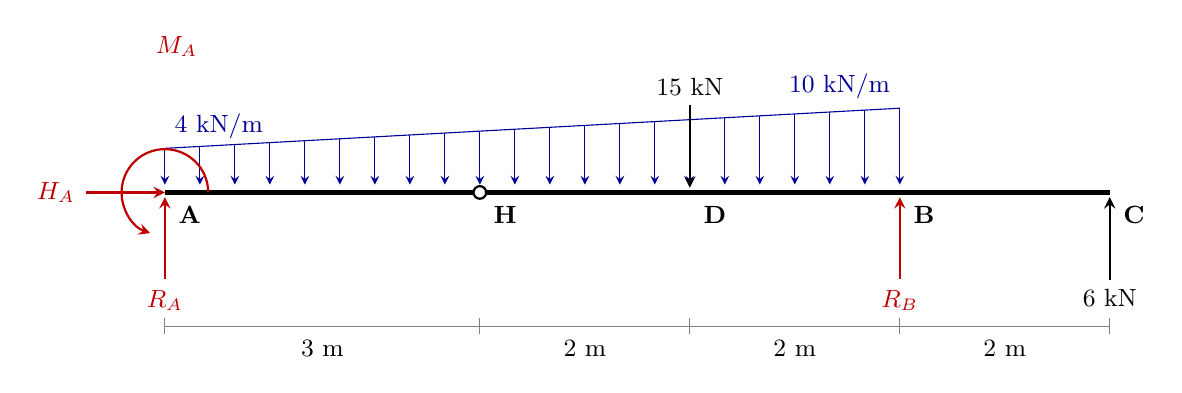
\begin{tikzpicture}
\draw[-stealth,blue!60!black] (0.0000,0.5600) -- (0.0000,0.1000);
\draw[-stealth,blue!60!black] (0.4444,0.5843) -- (0.4444,0.1000);
\draw[-stealth,blue!60!black] (0.8889,0.6086) -- (0.8889,0.1000);
\draw[-stealth,blue!60!black] (1.3333,0.6329) -- (1.3333,0.1000);
\draw[-stealth,blue!60!black] (1.7778,0.6571) -- (1.7778,0.1000);
\draw[-stealth,blue!60!black] (2.2222,0.6814) -- (2.2222,0.1000);
\draw[-stealth,blue!60!black] (2.6667,0.7057) -- (2.6667,0.1000);
\draw[-stealth,blue!60!black] (3.1111,0.7300) -- (3.1111,0.1000);
\draw[-stealth,blue!60!black] (3.5556,0.7543) -- (3.5556,0.1000);
\draw[-stealth,blue!60!black] (4.0000,0.7786) -- (4.0000,0.1000);
\draw[-stealth,blue!60!black] (4.4444,0.8029) -- (4.4444,0.1000);
\draw[-stealth,blue!60!black] (4.8889,0.8271) -- (4.8889,0.1000);
\draw[-stealth,blue!60!black] (5.3333,0.8514) -- (5.3333,0.1000);
\draw[-stealth,blue!60!black] (5.7778,0.8757) -- (5.7778,0.1000);
\draw[-stealth,blue!60!black] (6.2222,0.9000) -- (6.2222,0.1000);
\draw[-stealth,blue!60!black] (6.6667,0.9243) -- (6.6667,0.1000);
\draw[-stealth,blue!60!black] (7.1111,0.9486) -- (7.1111,0.1000);
\draw[-stealth,blue!60!black] (7.5556,0.9729) -- (7.5556,0.1000);
\draw[-stealth,blue!60!black] (8.0000,0.9971) -- (8.0000,0.1000);
\draw[-stealth,blue!60!black] (8.4444,1.0214) -- (8.4444,0.1000);
\draw[-stealth,blue!60!black] (8.8889,1.0457) -- (8.8889,0.1000);
\draw[-stealth,blue!60!black] (9.3333,1.0700) -- (9.3333,0.1000);
% studium:at distributed 0 x=0 to=7 check=span
\draw[blue!60!black] (0.0000,0.5600) -- (0.4444,0.5843) -- (0.8889,0.6086) -- (1.3333,0.6329) -- (1.7778,0.6571) -- (2.2222,0.6814) -- (2.6667,0.7057) -- (3.1111,0.7300) -- (3.5556,0.7543) -- (4.0000,0.7786) -- (4.4444,0.8029) -- (4.8889,0.8271) -- (5.3333,0.8514) -- (5.7778,0.8757) -- (6.2222,0.9000) -- (6.6667,0.9243) -- (7.1111,0.9486) -- (7.5556,0.9729) -- (8.0000,0.9971) -- (8.4444,1.0214) -- (8.8889,1.0457) -- (9.3333,1.0700);
\node[font=\small,anchor=south west,blue!60!black] at (0.0000,0.5600) {$4$~\mbox{kN/m}};
\node[font=\small,anchor=south east,blue!60!black] at (9.3333,1.0700) {$10$~\mbox{kN/m}};
\draw[line width=1.6pt] (0,0.0000) -- (12.0000,0.0000);
% studium:at hinge 0 x=3 check=first
\draw[thick,fill=white] (4.0000,0.0000) circle (0.08);
% studium:at force 0 x=5 check=tip
\draw[-stealth,thick,black] (6.6667,1.1100) -- (6.6667,0.0600);
\node[font=\small,anchor=south] at (6.6667,1.1100) {$15$~\mbox{kN}};
% studium:at force 1 x=9 check=tip
\draw[-stealth,thick,black] (12.0000,-1.1100) -- (12.0000,-0.0600);
\node[font=\small,anchor=north] at (12.0000,-1.1100) {$6$~\mbox{kN}};
% studium:at reaction H_A x=0 check=tip
\draw[-stealth,thick,red!75!black] (-1.0000,0.0000) -- (0.0000,0.0000);
\node[font=\small,anchor=east,red!75!black] at (-1.0200,0.0000) {$H_{A}$};
% studium:at reaction R_A x=0 check=tip
\draw[-stealth,thick,red!75!black] (0.0000,-1.1000) -- (0.0000,-0.0600);
\node[font=\small,anchor=north,red!75!black] at (0.0000,-1.1200) {$R_{A}$};
% studium:at reaction M_A x=0 check=arc
\draw[-stealth,thick,red!75!black] (0.5500,0.0000) arc (0:250:0.55);
\node[font=\small,anchor=south,red!75!black] at (0.1500,1.6000) {$M_{A}$};
% studium:at reaction R_B x=7 check=tip
\draw[-stealth,thick,red!75!black] (9.3333,-1.1000) -- (9.3333,-0.0600);
\node[font=\small,anchor=north,red!75!black] at (9.3333,-1.1200) {$R_{B}$};
\node[font=\small\bfseries,anchor=north west] at (0.0500,-0.0500) {A};
\node[font=\small\bfseries,anchor=north west] at (4.0500,-0.0500) {H};
\node[font=\small\bfseries,anchor=north west] at (6.7167,-0.0500) {D};
\node[font=\small\bfseries,anchor=north west] at (9.3833,-0.0500) {B};
\node[font=\small\bfseries,anchor=north west] at (12.0500,-0.0500) {C};
\draw[gray] (0,-1.7000) -- (12.0000,-1.7000);
\draw[gray] (0.0000,-1.8000) -- (0.0000,-1.6000);
\draw[gray] (4.0000,-1.8000) -- (4.0000,-1.6000);
\draw[gray] (6.6667,-1.8000) -- (6.6667,-1.6000);
\draw[gray] (9.3333,-1.8000) -- (9.3333,-1.6000);
\draw[gray] (12.0000,-1.8000) -- (12.0000,-1.6000);
\node[font=\small,anchor=north] at (2.0000,-1.7500) {$3$~\mbox{m}};
\node[font=\small,anchor=north] at (5.3333,-1.7500) {$2$~\mbox{m}};
\node[font=\small,anchor=north] at (8.0000,-1.7500) {$2$~\mbox{m}};
\node[font=\small,anchor=north] at (10.6667,-1.7500) {$2$~\mbox{m}};
\end{tikzpicture}%
\fi
\fi
\endgroup
\par\nopagebreak
\studiumcaption{fig:e2-c03-gerber-dsl}{Sólido libre: tres reacciones incógnita y la rótula, que aporta la cuarta ecuación.}
\end{minipage}\par\medskip

\par\medskip\noindent\begin{minipage}{\linewidth}
\centering
\begingroup
\setbox0=\hbox{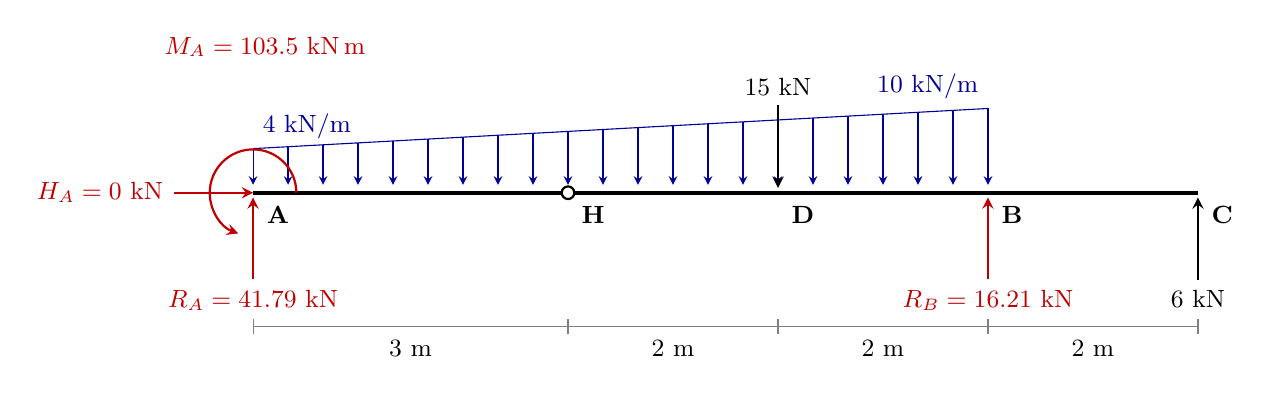
\begin{tikzpicture}
\draw[-stealth,blue!60!black] (0.0000,0.5600) -- (0.0000,0.1000);
\draw[-stealth,blue!60!black] (0.4444,0.5843) -- (0.4444,0.1000);
\draw[-stealth,blue!60!black] (0.8889,0.6086) -- (0.8889,0.1000);
\draw[-stealth,blue!60!black] (1.3333,0.6329) -- (1.3333,0.1000);
\draw[-stealth,blue!60!black] (1.7778,0.6571) -- (1.7778,0.1000);
\draw[-stealth,blue!60!black] (2.2222,0.6814) -- (2.2222,0.1000);
\draw[-stealth,blue!60!black] (2.6667,0.7057) -- (2.6667,0.1000);
\draw[-stealth,blue!60!black] (3.1111,0.7300) -- (3.1111,0.1000);
\draw[-stealth,blue!60!black] (3.5556,0.7543) -- (3.5556,0.1000);
\draw[-stealth,blue!60!black] (4.0000,0.7786) -- (4.0000,0.1000);
\draw[-stealth,blue!60!black] (4.4444,0.8029) -- (4.4444,0.1000);
\draw[-stealth,blue!60!black] (4.8889,0.8271) -- (4.8889,0.1000);
\draw[-stealth,blue!60!black] (5.3333,0.8514) -- (5.3333,0.1000);
\draw[-stealth,blue!60!black] (5.7778,0.8757) -- (5.7778,0.1000);
\draw[-stealth,blue!60!black] (6.2222,0.9000) -- (6.2222,0.1000);
\draw[-stealth,blue!60!black] (6.6667,0.9243) -- (6.6667,0.1000);
\draw[-stealth,blue!60!black] (7.1111,0.9486) -- (7.1111,0.1000);
\draw[-stealth,blue!60!black] (7.5556,0.9729) -- (7.5556,0.1000);
\draw[-stealth,blue!60!black] (8.0000,0.9971) -- (8.0000,0.1000);
\draw[-stealth,blue!60!black] (8.4444,1.0214) -- (8.4444,0.1000);
\draw[-stealth,blue!60!black] (8.8889,1.0457) -- (8.8889,0.1000);
\draw[-stealth,blue!60!black] (9.3333,1.0700) -- (9.3333,0.1000);
% studium:at distributed 0 x=0 to=7 check=span
\draw[blue!60!black] (0.0000,0.5600) -- (0.4444,0.5843) -- (0.8889,0.6086) -- (1.3333,0.6329) -- (1.7778,0.6571) -- (2.2222,0.6814) -- (2.6667,0.7057) -- (3.1111,0.7300) -- (3.5556,0.7543) -- (4.0000,0.7786) -- (4.4444,0.8029) -- (4.8889,0.8271) -- (5.3333,0.8514) -- (5.7778,0.8757) -- (6.2222,0.9000) -- (6.6667,0.9243) -- (7.1111,0.9486) -- (7.5556,0.9729) -- (8.0000,0.9971) -- (8.4444,1.0214) -- (8.8889,1.0457) -- (9.3333,1.0700);
\node[font=\small,anchor=south west,blue!60!black] at (0.0000,0.5600) {$4$~\mbox{kN/m}};
\node[font=\small,anchor=south east,blue!60!black] at (9.3333,1.0700) {$10$~\mbox{kN/m}};
\draw[line width=1.6pt] (0,0.0000) -- (12.0000,0.0000);
% studium:at hinge 0 x=3 check=first
\draw[thick,fill=white] (4.0000,0.0000) circle (0.08);
% studium:at force 0 x=5 check=tip
\draw[-stealth,thick,black] (6.6667,1.1100) -- (6.6667,0.0600);
\node[font=\small,anchor=south] at (6.6667,1.1100) {$15$~\mbox{kN}};
% studium:at force 1 x=9 check=tip
\draw[-stealth,thick,black] (12.0000,-1.1100) -- (12.0000,-0.0600);
\node[font=\small,anchor=north] at (12.0000,-1.1100) {$6$~\mbox{kN}};
% studium:reaction H_A value=0
% studium:at reaction H_A x=0 check=tip
\draw[-stealth,thick,red!75!black] (-1.0000,0.0000) -- (0.0000,0.0000);
\node[font=\small,anchor=east,red!75!black] at (-1.0200,0.0000) {$H_{A} = 0$~\mbox{kN}};
% studium:reaction R_A value=41.79
% studium:at reaction R_A x=0 check=tip
\draw[-stealth,thick,red!75!black] (0.0000,-1.1000) -- (0.0000,-0.0600);
\node[font=\small,anchor=north,red!75!black] at (0.0000,-1.1200) {$R_{A} = 41.79$~\mbox{kN}};
% studium:reaction M_A value=103.5
% studium:at reaction M_A x=0 check=arc
\draw[-stealth,thick,red!75!black] (0.5500,0.0000) arc (0:250:0.55);
\node[font=\small,anchor=south,red!75!black] at (0.1500,1.6000) {$M_{A} = 103.5$~\mbox{kN\,m}};
% studium:reaction R_B value=16.21
% studium:at reaction R_B x=7 check=tip
\draw[-stealth,thick,red!75!black] (9.3333,-1.1000) -- (9.3333,-0.0600);
\node[font=\small,anchor=north,red!75!black] at (9.3333,-1.1200) {$R_{B} = 16.21$~\mbox{kN}};
\node[font=\small\bfseries,anchor=north west] at (0.0500,-0.0500) {A};
\node[font=\small\bfseries,anchor=north west] at (4.0500,-0.0500) {H};
\node[font=\small\bfseries,anchor=north west] at (6.7167,-0.0500) {D};
\node[font=\small\bfseries,anchor=north west] at (9.3833,-0.0500) {B};
\node[font=\small\bfseries,anchor=north west] at (12.0500,-0.0500) {C};
\draw[gray] (0,-1.7000) -- (12.0000,-1.7000);
\draw[gray] (0.0000,-1.8000) -- (0.0000,-1.6000);
\draw[gray] (4.0000,-1.8000) -- (4.0000,-1.6000);
\draw[gray] (6.6667,-1.8000) -- (6.6667,-1.6000);
\draw[gray] (9.3333,-1.8000) -- (9.3333,-1.6000);
\draw[gray] (12.0000,-1.8000) -- (12.0000,-1.6000);
\node[font=\small,anchor=north] at (2.0000,-1.7500) {$3$~\mbox{m}};
\node[font=\small,anchor=north] at (5.3333,-1.7500) {$2$~\mbox{m}};
\node[font=\small,anchor=north] at (8.0000,-1.7500) {$2$~\mbox{m}};
\node[font=\small,anchor=north] at (10.6667,-1.7500) {$2$~\mbox{m}};
\end{tikzpicture}}%
\count0=\ht0
\advance\count0 by \dp0
\count2=\wd0
\count4=\dimexpr\textheight/100*38\relax
\count6=\linewidth
\ifnum\count0<1
\count0=1
\fi
\ifnum\count2<1
\count2=1
\fi
\divide\count0 by 4096
\divide\count2 by 4096
\divide\count4 by 4096
\divide\count6 by 4096
\ifnum\count0<1
\count0=1
\fi
\ifnum\count2<1
\count2=1
\fi
\ifnum\count4<1
\count4=1
\fi
\ifnum\count6<1
\count6=1
\fi
\count8=\count2
\ifnum\count0>\count4
\count8=\numexpr\count2*\count4/\count0\relax
\fi
\ifnum\count8>\count6
\resizebox{\linewidth}{!}{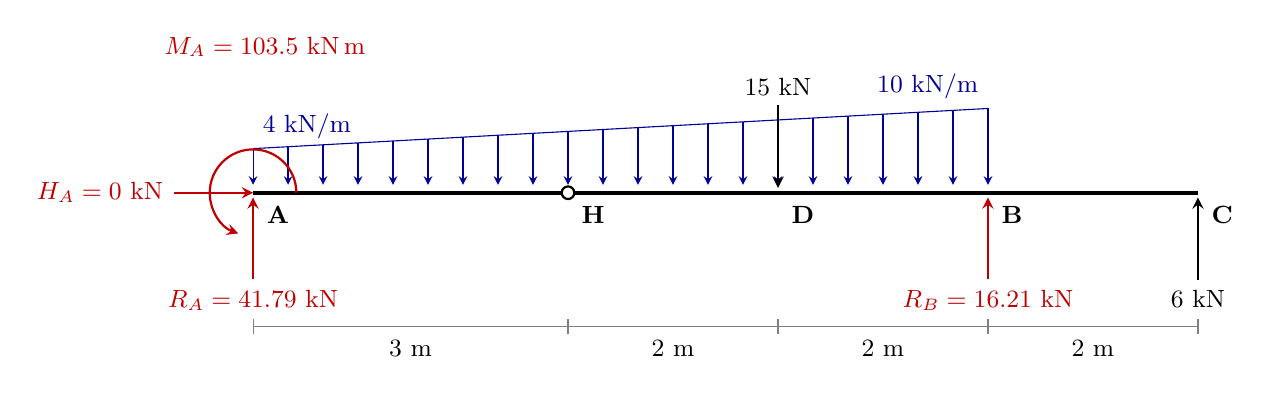
\begin{tikzpicture}
\draw[-stealth,blue!60!black] (0.0000,0.5600) -- (0.0000,0.1000);
\draw[-stealth,blue!60!black] (0.4444,0.5843) -- (0.4444,0.1000);
\draw[-stealth,blue!60!black] (0.8889,0.6086) -- (0.8889,0.1000);
\draw[-stealth,blue!60!black] (1.3333,0.6329) -- (1.3333,0.1000);
\draw[-stealth,blue!60!black] (1.7778,0.6571) -- (1.7778,0.1000);
\draw[-stealth,blue!60!black] (2.2222,0.6814) -- (2.2222,0.1000);
\draw[-stealth,blue!60!black] (2.6667,0.7057) -- (2.6667,0.1000);
\draw[-stealth,blue!60!black] (3.1111,0.7300) -- (3.1111,0.1000);
\draw[-stealth,blue!60!black] (3.5556,0.7543) -- (3.5556,0.1000);
\draw[-stealth,blue!60!black] (4.0000,0.7786) -- (4.0000,0.1000);
\draw[-stealth,blue!60!black] (4.4444,0.8029) -- (4.4444,0.1000);
\draw[-stealth,blue!60!black] (4.8889,0.8271) -- (4.8889,0.1000);
\draw[-stealth,blue!60!black] (5.3333,0.8514) -- (5.3333,0.1000);
\draw[-stealth,blue!60!black] (5.7778,0.8757) -- (5.7778,0.1000);
\draw[-stealth,blue!60!black] (6.2222,0.9000) -- (6.2222,0.1000);
\draw[-stealth,blue!60!black] (6.6667,0.9243) -- (6.6667,0.1000);
\draw[-stealth,blue!60!black] (7.1111,0.9486) -- (7.1111,0.1000);
\draw[-stealth,blue!60!black] (7.5556,0.9729) -- (7.5556,0.1000);
\draw[-stealth,blue!60!black] (8.0000,0.9971) -- (8.0000,0.1000);
\draw[-stealth,blue!60!black] (8.4444,1.0214) -- (8.4444,0.1000);
\draw[-stealth,blue!60!black] (8.8889,1.0457) -- (8.8889,0.1000);
\draw[-stealth,blue!60!black] (9.3333,1.0700) -- (9.3333,0.1000);
% studium:at distributed 0 x=0 to=7 check=span
\draw[blue!60!black] (0.0000,0.5600) -- (0.4444,0.5843) -- (0.8889,0.6086) -- (1.3333,0.6329) -- (1.7778,0.6571) -- (2.2222,0.6814) -- (2.6667,0.7057) -- (3.1111,0.7300) -- (3.5556,0.7543) -- (4.0000,0.7786) -- (4.4444,0.8029) -- (4.8889,0.8271) -- (5.3333,0.8514) -- (5.7778,0.8757) -- (6.2222,0.9000) -- (6.6667,0.9243) -- (7.1111,0.9486) -- (7.5556,0.9729) -- (8.0000,0.9971) -- (8.4444,1.0214) -- (8.8889,1.0457) -- (9.3333,1.0700);
\node[font=\small,anchor=south west,blue!60!black] at (0.0000,0.5600) {$4$~\mbox{kN/m}};
\node[font=\small,anchor=south east,blue!60!black] at (9.3333,1.0700) {$10$~\mbox{kN/m}};
\draw[line width=1.6pt] (0,0.0000) -- (12.0000,0.0000);
% studium:at hinge 0 x=3 check=first
\draw[thick,fill=white] (4.0000,0.0000) circle (0.08);
% studium:at force 0 x=5 check=tip
\draw[-stealth,thick,black] (6.6667,1.1100) -- (6.6667,0.0600);
\node[font=\small,anchor=south] at (6.6667,1.1100) {$15$~\mbox{kN}};
% studium:at force 1 x=9 check=tip
\draw[-stealth,thick,black] (12.0000,-1.1100) -- (12.0000,-0.0600);
\node[font=\small,anchor=north] at (12.0000,-1.1100) {$6$~\mbox{kN}};
% studium:reaction H_A value=0
% studium:at reaction H_A x=0 check=tip
\draw[-stealth,thick,red!75!black] (-1.0000,0.0000) -- (0.0000,0.0000);
\node[font=\small,anchor=east,red!75!black] at (-1.0200,0.0000) {$H_{A} = 0$~\mbox{kN}};
% studium:reaction R_A value=41.79
% studium:at reaction R_A x=0 check=tip
\draw[-stealth,thick,red!75!black] (0.0000,-1.1000) -- (0.0000,-0.0600);
\node[font=\small,anchor=north,red!75!black] at (0.0000,-1.1200) {$R_{A} = 41.79$~\mbox{kN}};
% studium:reaction M_A value=103.5
% studium:at reaction M_A x=0 check=arc
\draw[-stealth,thick,red!75!black] (0.5500,0.0000) arc (0:250:0.55);
\node[font=\small,anchor=south,red!75!black] at (0.1500,1.6000) {$M_{A} = 103.5$~\mbox{kN\,m}};
% studium:reaction R_B value=16.21
% studium:at reaction R_B x=7 check=tip
\draw[-stealth,thick,red!75!black] (9.3333,-1.1000) -- (9.3333,-0.0600);
\node[font=\small,anchor=north,red!75!black] at (9.3333,-1.1200) {$R_{B} = 16.21$~\mbox{kN}};
\node[font=\small\bfseries,anchor=north west] at (0.0500,-0.0500) {A};
\node[font=\small\bfseries,anchor=north west] at (4.0500,-0.0500) {H};
\node[font=\small\bfseries,anchor=north west] at (6.7167,-0.0500) {D};
\node[font=\small\bfseries,anchor=north west] at (9.3833,-0.0500) {B};
\node[font=\small\bfseries,anchor=north west] at (12.0500,-0.0500) {C};
\draw[gray] (0,-1.7000) -- (12.0000,-1.7000);
\draw[gray] (0.0000,-1.8000) -- (0.0000,-1.6000);
\draw[gray] (4.0000,-1.8000) -- (4.0000,-1.6000);
\draw[gray] (6.6667,-1.8000) -- (6.6667,-1.6000);
\draw[gray] (9.3333,-1.8000) -- (9.3333,-1.6000);
\draw[gray] (12.0000,-1.8000) -- (12.0000,-1.6000);
\node[font=\small,anchor=north] at (2.0000,-1.7500) {$3$~\mbox{m}};
\node[font=\small,anchor=north] at (5.3333,-1.7500) {$2$~\mbox{m}};
\node[font=\small,anchor=north] at (8.0000,-1.7500) {$2$~\mbox{m}};
\node[font=\small,anchor=north] at (10.6667,-1.7500) {$2$~\mbox{m}};
\end{tikzpicture}}%
\else
\ifnum\count0>\count4
\resizebox{!}{\dimexpr\textheight/100*38\relax}{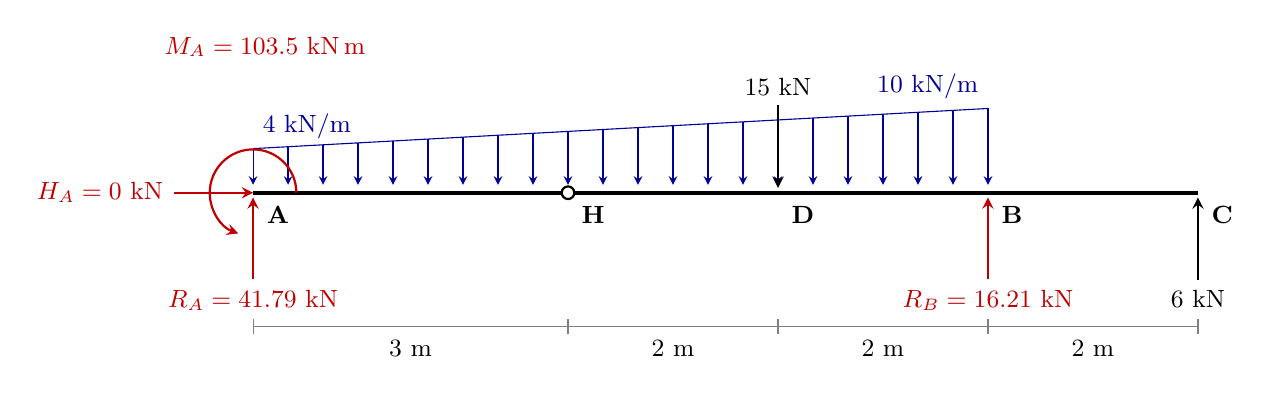
\begin{tikzpicture}
\draw[-stealth,blue!60!black] (0.0000,0.5600) -- (0.0000,0.1000);
\draw[-stealth,blue!60!black] (0.4444,0.5843) -- (0.4444,0.1000);
\draw[-stealth,blue!60!black] (0.8889,0.6086) -- (0.8889,0.1000);
\draw[-stealth,blue!60!black] (1.3333,0.6329) -- (1.3333,0.1000);
\draw[-stealth,blue!60!black] (1.7778,0.6571) -- (1.7778,0.1000);
\draw[-stealth,blue!60!black] (2.2222,0.6814) -- (2.2222,0.1000);
\draw[-stealth,blue!60!black] (2.6667,0.7057) -- (2.6667,0.1000);
\draw[-stealth,blue!60!black] (3.1111,0.7300) -- (3.1111,0.1000);
\draw[-stealth,blue!60!black] (3.5556,0.7543) -- (3.5556,0.1000);
\draw[-stealth,blue!60!black] (4.0000,0.7786) -- (4.0000,0.1000);
\draw[-stealth,blue!60!black] (4.4444,0.8029) -- (4.4444,0.1000);
\draw[-stealth,blue!60!black] (4.8889,0.8271) -- (4.8889,0.1000);
\draw[-stealth,blue!60!black] (5.3333,0.8514) -- (5.3333,0.1000);
\draw[-stealth,blue!60!black] (5.7778,0.8757) -- (5.7778,0.1000);
\draw[-stealth,blue!60!black] (6.2222,0.9000) -- (6.2222,0.1000);
\draw[-stealth,blue!60!black] (6.6667,0.9243) -- (6.6667,0.1000);
\draw[-stealth,blue!60!black] (7.1111,0.9486) -- (7.1111,0.1000);
\draw[-stealth,blue!60!black] (7.5556,0.9729) -- (7.5556,0.1000);
\draw[-stealth,blue!60!black] (8.0000,0.9971) -- (8.0000,0.1000);
\draw[-stealth,blue!60!black] (8.4444,1.0214) -- (8.4444,0.1000);
\draw[-stealth,blue!60!black] (8.8889,1.0457) -- (8.8889,0.1000);
\draw[-stealth,blue!60!black] (9.3333,1.0700) -- (9.3333,0.1000);
% studium:at distributed 0 x=0 to=7 check=span
\draw[blue!60!black] (0.0000,0.5600) -- (0.4444,0.5843) -- (0.8889,0.6086) -- (1.3333,0.6329) -- (1.7778,0.6571) -- (2.2222,0.6814) -- (2.6667,0.7057) -- (3.1111,0.7300) -- (3.5556,0.7543) -- (4.0000,0.7786) -- (4.4444,0.8029) -- (4.8889,0.8271) -- (5.3333,0.8514) -- (5.7778,0.8757) -- (6.2222,0.9000) -- (6.6667,0.9243) -- (7.1111,0.9486) -- (7.5556,0.9729) -- (8.0000,0.9971) -- (8.4444,1.0214) -- (8.8889,1.0457) -- (9.3333,1.0700);
\node[font=\small,anchor=south west,blue!60!black] at (0.0000,0.5600) {$4$~\mbox{kN/m}};
\node[font=\small,anchor=south east,blue!60!black] at (9.3333,1.0700) {$10$~\mbox{kN/m}};
\draw[line width=1.6pt] (0,0.0000) -- (12.0000,0.0000);
% studium:at hinge 0 x=3 check=first
\draw[thick,fill=white] (4.0000,0.0000) circle (0.08);
% studium:at force 0 x=5 check=tip
\draw[-stealth,thick,black] (6.6667,1.1100) -- (6.6667,0.0600);
\node[font=\small,anchor=south] at (6.6667,1.1100) {$15$~\mbox{kN}};
% studium:at force 1 x=9 check=tip
\draw[-stealth,thick,black] (12.0000,-1.1100) -- (12.0000,-0.0600);
\node[font=\small,anchor=north] at (12.0000,-1.1100) {$6$~\mbox{kN}};
% studium:reaction H_A value=0
% studium:at reaction H_A x=0 check=tip
\draw[-stealth,thick,red!75!black] (-1.0000,0.0000) -- (0.0000,0.0000);
\node[font=\small,anchor=east,red!75!black] at (-1.0200,0.0000) {$H_{A} = 0$~\mbox{kN}};
% studium:reaction R_A value=41.79
% studium:at reaction R_A x=0 check=tip
\draw[-stealth,thick,red!75!black] (0.0000,-1.1000) -- (0.0000,-0.0600);
\node[font=\small,anchor=north,red!75!black] at (0.0000,-1.1200) {$R_{A} = 41.79$~\mbox{kN}};
% studium:reaction M_A value=103.5
% studium:at reaction M_A x=0 check=arc
\draw[-stealth,thick,red!75!black] (0.5500,0.0000) arc (0:250:0.55);
\node[font=\small,anchor=south,red!75!black] at (0.1500,1.6000) {$M_{A} = 103.5$~\mbox{kN\,m}};
% studium:reaction R_B value=16.21
% studium:at reaction R_B x=7 check=tip
\draw[-stealth,thick,red!75!black] (9.3333,-1.1000) -- (9.3333,-0.0600);
\node[font=\small,anchor=north,red!75!black] at (9.3333,-1.1200) {$R_{B} = 16.21$~\mbox{kN}};
\node[font=\small\bfseries,anchor=north west] at (0.0500,-0.0500) {A};
\node[font=\small\bfseries,anchor=north west] at (4.0500,-0.0500) {H};
\node[font=\small\bfseries,anchor=north west] at (6.7167,-0.0500) {D};
\node[font=\small\bfseries,anchor=north west] at (9.3833,-0.0500) {B};
\node[font=\small\bfseries,anchor=north west] at (12.0500,-0.0500) {C};
\draw[gray] (0,-1.7000) -- (12.0000,-1.7000);
\draw[gray] (0.0000,-1.8000) -- (0.0000,-1.6000);
\draw[gray] (4.0000,-1.8000) -- (4.0000,-1.6000);
\draw[gray] (6.6667,-1.8000) -- (6.6667,-1.6000);
\draw[gray] (9.3333,-1.8000) -- (9.3333,-1.6000);
\draw[gray] (12.0000,-1.8000) -- (12.0000,-1.6000);
\node[font=\small,anchor=north] at (2.0000,-1.7500) {$3$~\mbox{m}};
\node[font=\small,anchor=north] at (5.3333,-1.7500) {$2$~\mbox{m}};
\node[font=\small,anchor=north] at (8.0000,-1.7500) {$2$~\mbox{m}};
\node[font=\small,anchor=north] at (10.6667,-1.7500) {$2$~\mbox{m}};
\end{tikzpicture}}%
\else
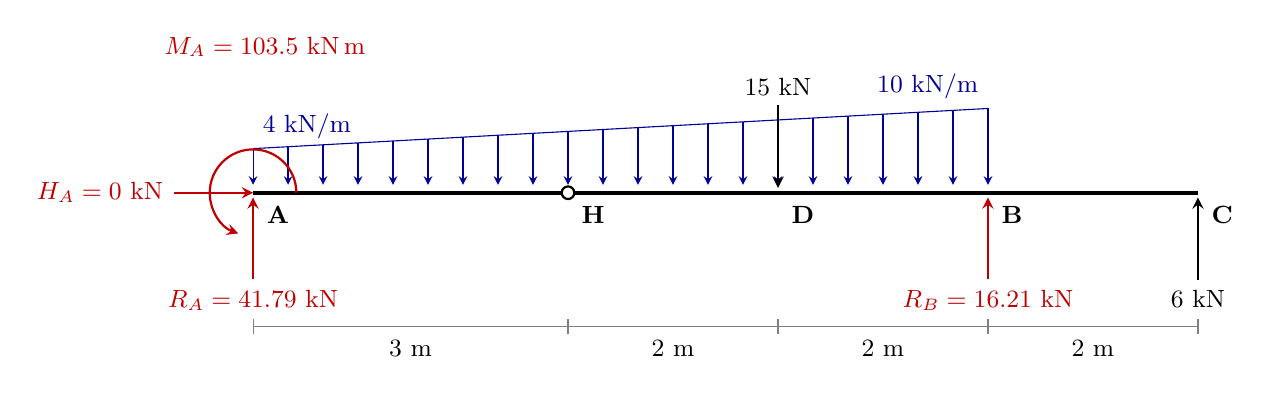
\begin{tikzpicture}
\draw[-stealth,blue!60!black] (0.0000,0.5600) -- (0.0000,0.1000);
\draw[-stealth,blue!60!black] (0.4444,0.5843) -- (0.4444,0.1000);
\draw[-stealth,blue!60!black] (0.8889,0.6086) -- (0.8889,0.1000);
\draw[-stealth,blue!60!black] (1.3333,0.6329) -- (1.3333,0.1000);
\draw[-stealth,blue!60!black] (1.7778,0.6571) -- (1.7778,0.1000);
\draw[-stealth,blue!60!black] (2.2222,0.6814) -- (2.2222,0.1000);
\draw[-stealth,blue!60!black] (2.6667,0.7057) -- (2.6667,0.1000);
\draw[-stealth,blue!60!black] (3.1111,0.7300) -- (3.1111,0.1000);
\draw[-stealth,blue!60!black] (3.5556,0.7543) -- (3.5556,0.1000);
\draw[-stealth,blue!60!black] (4.0000,0.7786) -- (4.0000,0.1000);
\draw[-stealth,blue!60!black] (4.4444,0.8029) -- (4.4444,0.1000);
\draw[-stealth,blue!60!black] (4.8889,0.8271) -- (4.8889,0.1000);
\draw[-stealth,blue!60!black] (5.3333,0.8514) -- (5.3333,0.1000);
\draw[-stealth,blue!60!black] (5.7778,0.8757) -- (5.7778,0.1000);
\draw[-stealth,blue!60!black] (6.2222,0.9000) -- (6.2222,0.1000);
\draw[-stealth,blue!60!black] (6.6667,0.9243) -- (6.6667,0.1000);
\draw[-stealth,blue!60!black] (7.1111,0.9486) -- (7.1111,0.1000);
\draw[-stealth,blue!60!black] (7.5556,0.9729) -- (7.5556,0.1000);
\draw[-stealth,blue!60!black] (8.0000,0.9971) -- (8.0000,0.1000);
\draw[-stealth,blue!60!black] (8.4444,1.0214) -- (8.4444,0.1000);
\draw[-stealth,blue!60!black] (8.8889,1.0457) -- (8.8889,0.1000);
\draw[-stealth,blue!60!black] (9.3333,1.0700) -- (9.3333,0.1000);
% studium:at distributed 0 x=0 to=7 check=span
\draw[blue!60!black] (0.0000,0.5600) -- (0.4444,0.5843) -- (0.8889,0.6086) -- (1.3333,0.6329) -- (1.7778,0.6571) -- (2.2222,0.6814) -- (2.6667,0.7057) -- (3.1111,0.7300) -- (3.5556,0.7543) -- (4.0000,0.7786) -- (4.4444,0.8029) -- (4.8889,0.8271) -- (5.3333,0.8514) -- (5.7778,0.8757) -- (6.2222,0.9000) -- (6.6667,0.9243) -- (7.1111,0.9486) -- (7.5556,0.9729) -- (8.0000,0.9971) -- (8.4444,1.0214) -- (8.8889,1.0457) -- (9.3333,1.0700);
\node[font=\small,anchor=south west,blue!60!black] at (0.0000,0.5600) {$4$~\mbox{kN/m}};
\node[font=\small,anchor=south east,blue!60!black] at (9.3333,1.0700) {$10$~\mbox{kN/m}};
\draw[line width=1.6pt] (0,0.0000) -- (12.0000,0.0000);
% studium:at hinge 0 x=3 check=first
\draw[thick,fill=white] (4.0000,0.0000) circle (0.08);
% studium:at force 0 x=5 check=tip
\draw[-stealth,thick,black] (6.6667,1.1100) -- (6.6667,0.0600);
\node[font=\small,anchor=south] at (6.6667,1.1100) {$15$~\mbox{kN}};
% studium:at force 1 x=9 check=tip
\draw[-stealth,thick,black] (12.0000,-1.1100) -- (12.0000,-0.0600);
\node[font=\small,anchor=north] at (12.0000,-1.1100) {$6$~\mbox{kN}};
% studium:reaction H_A value=0
% studium:at reaction H_A x=0 check=tip
\draw[-stealth,thick,red!75!black] (-1.0000,0.0000) -- (0.0000,0.0000);
\node[font=\small,anchor=east,red!75!black] at (-1.0200,0.0000) {$H_{A} = 0$~\mbox{kN}};
% studium:reaction R_A value=41.79
% studium:at reaction R_A x=0 check=tip
\draw[-stealth,thick,red!75!black] (0.0000,-1.1000) -- (0.0000,-0.0600);
\node[font=\small,anchor=north,red!75!black] at (0.0000,-1.1200) {$R_{A} = 41.79$~\mbox{kN}};
% studium:reaction M_A value=103.5
% studium:at reaction M_A x=0 check=arc
\draw[-stealth,thick,red!75!black] (0.5500,0.0000) arc (0:250:0.55);
\node[font=\small,anchor=south,red!75!black] at (0.1500,1.6000) {$M_{A} = 103.5$~\mbox{kN\,m}};
% studium:reaction R_B value=16.21
% studium:at reaction R_B x=7 check=tip
\draw[-stealth,thick,red!75!black] (9.3333,-1.1000) -- (9.3333,-0.0600);
\node[font=\small,anchor=north,red!75!black] at (9.3333,-1.1200) {$R_{B} = 16.21$~\mbox{kN}};
\node[font=\small\bfseries,anchor=north west] at (0.0500,-0.0500) {A};
\node[font=\small\bfseries,anchor=north west] at (4.0500,-0.0500) {H};
\node[font=\small\bfseries,anchor=north west] at (6.7167,-0.0500) {D};
\node[font=\small\bfseries,anchor=north west] at (9.3833,-0.0500) {B};
\node[font=\small\bfseries,anchor=north west] at (12.0500,-0.0500) {C};
\draw[gray] (0,-1.7000) -- (12.0000,-1.7000);
\draw[gray] (0.0000,-1.8000) -- (0.0000,-1.6000);
\draw[gray] (4.0000,-1.8000) -- (4.0000,-1.6000);
\draw[gray] (6.6667,-1.8000) -- (6.6667,-1.6000);
\draw[gray] (9.3333,-1.8000) -- (9.3333,-1.6000);
\draw[gray] (12.0000,-1.8000) -- (12.0000,-1.6000);
\node[font=\small,anchor=north] at (2.0000,-1.7500) {$3$~\mbox{m}};
\node[font=\small,anchor=north] at (5.3333,-1.7500) {$2$~\mbox{m}};
\node[font=\small,anchor=north] at (8.0000,-1.7500) {$2$~\mbox{m}};
\node[font=\small,anchor=north] at (10.6667,-1.7500) {$2$~\mbox{m}};
\end{tikzpicture}%
\fi
\fi
\endgroup
\par\nopagebreak
\studiumcaption{fig:e2-c03-gerber-reacciones}{Reacciones obtenidas. El signo de cada valor se refiere al sentido dibujado: \(M_A\) negativo es un momento horario.}
\end{minipage}\par\medskip

\par\medskip\noindent\begin{minipage}{\linewidth}
\centering
\begingroup
\setbox0=\hbox{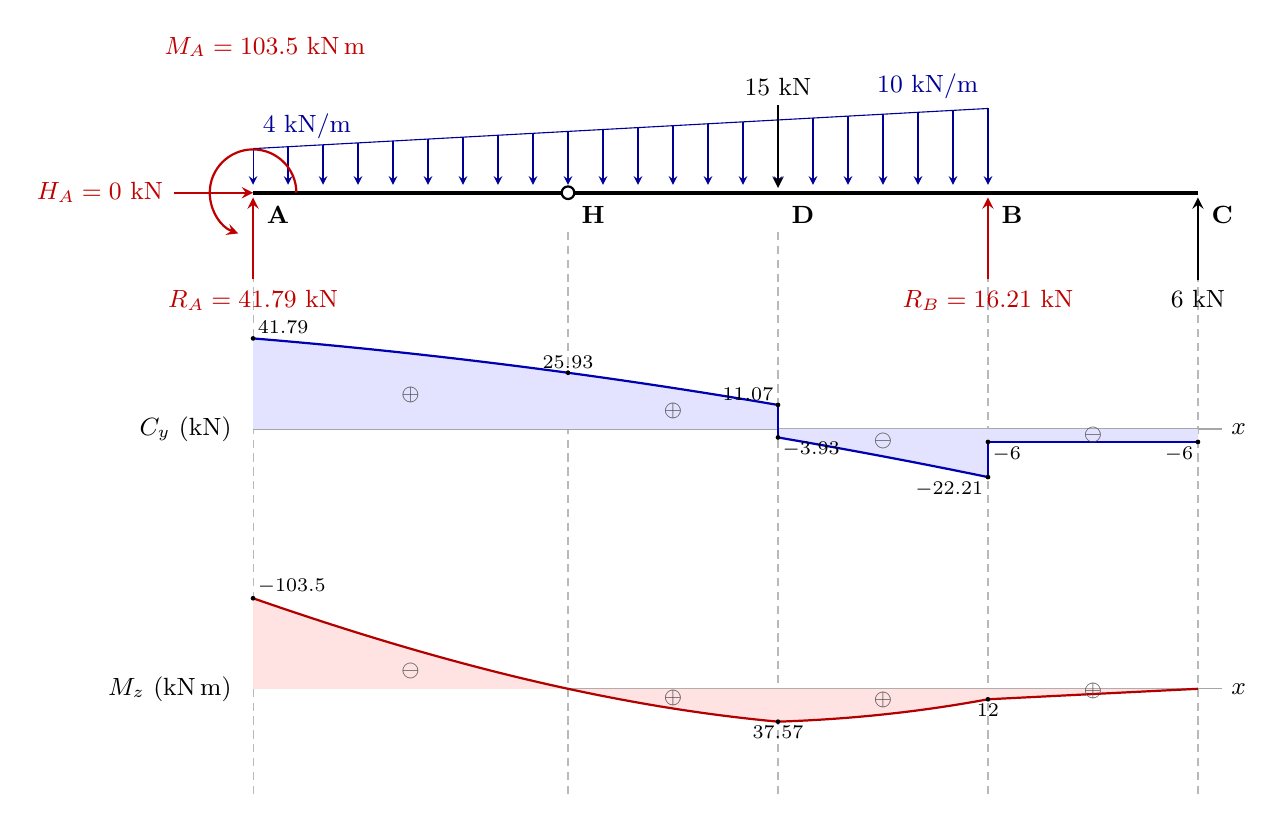
\begin{tikzpicture}
\draw[densely dashed,gray!55] (12.0000,-0.5000) -- (12.0000,-7.7000);
\draw[densely dashed,gray!55] (9.3333,-0.5000) -- (9.3333,-7.7000);
\draw[densely dashed,gray!55] (6.6667,-0.5000) -- (6.6667,-7.7000);
\draw[densely dashed,gray!55] (4.0000,-0.5000) -- (4.0000,-7.7000);
\draw[densely dashed,gray!55] (0.0000,-0.5000) -- (0.0000,-7.7000);
\draw[-stealth,blue!60!black] (0.0000,0.5600) -- (0.0000,0.1000);
\draw[-stealth,blue!60!black] (0.4444,0.5843) -- (0.4444,0.1000);
\draw[-stealth,blue!60!black] (0.8889,0.6086) -- (0.8889,0.1000);
\draw[-stealth,blue!60!black] (1.3333,0.6329) -- (1.3333,0.1000);
\draw[-stealth,blue!60!black] (1.7778,0.6571) -- (1.7778,0.1000);
\draw[-stealth,blue!60!black] (2.2222,0.6814) -- (2.2222,0.1000);
\draw[-stealth,blue!60!black] (2.6667,0.7057) -- (2.6667,0.1000);
\draw[-stealth,blue!60!black] (3.1111,0.7300) -- (3.1111,0.1000);
\draw[-stealth,blue!60!black] (3.5556,0.7543) -- (3.5556,0.1000);
\draw[-stealth,blue!60!black] (4.0000,0.7786) -- (4.0000,0.1000);
\draw[-stealth,blue!60!black] (4.4444,0.8029) -- (4.4444,0.1000);
\draw[-stealth,blue!60!black] (4.8889,0.8271) -- (4.8889,0.1000);
\draw[-stealth,blue!60!black] (5.3333,0.8514) -- (5.3333,0.1000);
\draw[-stealth,blue!60!black] (5.7778,0.8757) -- (5.7778,0.1000);
\draw[-stealth,blue!60!black] (6.2222,0.9000) -- (6.2222,0.1000);
\draw[-stealth,blue!60!black] (6.6667,0.9243) -- (6.6667,0.1000);
\draw[-stealth,blue!60!black] (7.1111,0.9486) -- (7.1111,0.1000);
\draw[-stealth,blue!60!black] (7.5556,0.9729) -- (7.5556,0.1000);
\draw[-stealth,blue!60!black] (8.0000,0.9971) -- (8.0000,0.1000);
\draw[-stealth,blue!60!black] (8.4444,1.0214) -- (8.4444,0.1000);
\draw[-stealth,blue!60!black] (8.8889,1.0457) -- (8.8889,0.1000);
\draw[-stealth,blue!60!black] (9.3333,1.0700) -- (9.3333,0.1000);
% studium:at distributed 0 x=0 to=7 check=span
\draw[blue!60!black] (0.0000,0.5600) -- (0.4444,0.5843) -- (0.8889,0.6086) -- (1.3333,0.6329) -- (1.7778,0.6571) -- (2.2222,0.6814) -- (2.6667,0.7057) -- (3.1111,0.7300) -- (3.5556,0.7543) -- (4.0000,0.7786) -- (4.4444,0.8029) -- (4.8889,0.8271) -- (5.3333,0.8514) -- (5.7778,0.8757) -- (6.2222,0.9000) -- (6.6667,0.9243) -- (7.1111,0.9486) -- (7.5556,0.9729) -- (8.0000,0.9971) -- (8.4444,1.0214) -- (8.8889,1.0457) -- (9.3333,1.0700);
\node[font=\small,anchor=south west,blue!60!black] at (0.0000,0.5600) {$4$~\mbox{kN/m}};
\node[font=\small,anchor=south east,blue!60!black] at (9.3333,1.0700) {$10$~\mbox{kN/m}};
\draw[line width=1.6pt] (0,0.0000) -- (12.0000,0.0000);
% studium:at hinge 0 x=3 check=first
\draw[thick,fill=white] (4.0000,0.0000) circle (0.08);
% studium:at force 0 x=5 check=tip
\draw[-stealth,thick,black] (6.6667,1.1100) -- (6.6667,0.0600);
\node[font=\small,anchor=south] at (6.6667,1.1100) {$15$~\mbox{kN}};
% studium:at force 1 x=9 check=tip
\draw[-stealth,thick,black] (12.0000,-1.1100) -- (12.0000,-0.0600);
\node[font=\small,anchor=north] at (12.0000,-1.1100) {$6$~\mbox{kN}};
% studium:reaction H_A value=0
% studium:at reaction H_A x=0 check=tip
\draw[-stealth,thick,red!75!black] (-1.0000,0.0000) -- (0.0000,0.0000);
\node[font=\small,anchor=east,red!75!black] at (-1.0200,0.0000) {$H_{A} = 0$~\mbox{kN}};
% studium:reaction R_A value=41.79
% studium:at reaction R_A x=0 check=tip
\draw[-stealth,thick,red!75!black] (0.0000,-1.1000) -- (0.0000,-0.0600);
\node[font=\small,anchor=north,red!75!black] at (0.0000,-1.1200) {$R_{A} = 41.79$~\mbox{kN}};
% studium:reaction M_A value=103.5
% studium:at reaction M_A x=0 check=arc
\draw[-stealth,thick,red!75!black] (0.5500,0.0000) arc (0:250:0.55);
\node[font=\small,anchor=south,red!75!black] at (0.1500,1.6000) {$M_{A} = 103.5$~\mbox{kN\,m}};
% studium:reaction R_B value=16.21
% studium:at reaction R_B x=7 check=tip
\draw[-stealth,thick,red!75!black] (9.3333,-1.1000) -- (9.3333,-0.0600);
\node[font=\small,anchor=north,red!75!black] at (9.3333,-1.1200) {$R_{B} = 16.21$~\mbox{kN}};
\node[font=\small\bfseries,anchor=north west] at (0.0500,-0.0500) {A};
\node[font=\small\bfseries,anchor=north west] at (4.0500,-0.0500) {H};
\node[font=\small\bfseries,anchor=north west] at (6.7167,-0.0500) {D};
\node[font=\small\bfseries,anchor=north west] at (9.3833,-0.0500) {B};
\node[font=\small\bfseries,anchor=north west] at (12.0500,-0.0500) {C};
\draw[gray!70] (0,-3.0000) -- (12.3000,-3.0000);
\fill[blue!11] (0.0000,-3.0000) -- (0.0000,-1.8500) -- (0.1250,-1.8604) -- (0.2500,-1.8711) -- (0.3750,-1.8819) -- (0.5000,-1.8929) -- (0.6250,-1.9042) -- (0.7500,-1.9157) -- (0.8750,-1.9273) -- (1.0000,-1.9392) -- (1.1250,-1.9513) -- (1.2500,-1.9636) -- (1.3750,-1.9761) -- (1.5000,-1.9888) -- (1.6250,-2.0017) -- (1.7500,-2.0148) -- (1.8750,-2.0281) -- (2.0000,-2.0417) -- (2.1250,-2.0554) -- (2.2500,-2.0694) -- (2.3750,-2.0835) -- (2.5000,-2.0979) -- (2.6250,-2.1124) -- (2.7500,-2.1272) -- (2.8750,-2.1422) -- (3.0000,-2.1574) -- (3.1250,-2.1728) -- (3.2500,-2.1884) -- (3.3750,-2.2042) -- (3.5000,-2.2202) -- (3.6250,-2.2365) -- (3.7500,-2.2529) -- (3.8750,-2.2696) -- (4.0000,-2.2864) -- (4.0000,-3.0000) -- cycle;
\fill[blue!11] (4.0000,-3.0000) -- (4.0000,-2.2864) -- (4.0833,-2.2978) -- (4.1667,-2.3092) -- (4.2500,-2.3207) -- (4.3333,-2.3324) -- (4.4167,-2.3441) -- (4.5000,-2.3559) -- (4.5833,-2.3678) -- (4.6667,-2.3798) -- (4.7500,-2.3919) -- (4.8333,-2.4041) -- (4.9167,-2.4163) -- (5.0000,-2.4287) -- (5.0833,-2.4411) -- (5.1667,-2.4537) -- (5.2500,-2.4663) -- (5.3333,-2.4791) -- (5.4167,-2.4919) -- (5.5000,-2.5048) -- (5.5833,-2.5178) -- (5.6667,-2.5309) -- (5.7500,-2.5441) -- (5.8333,-2.5574) -- (5.9167,-2.5708) -- (6.0000,-2.5842) -- (6.0833,-2.5978) -- (6.1667,-2.6114) -- (6.2500,-2.6252) -- (6.3333,-2.6390) -- (6.4167,-2.6530) -- (6.5000,-2.6670) -- (6.5833,-2.6811) -- (6.6667,-2.6953) -- (6.6667,-3.0000) -- cycle;
\fill[blue!11] (6.6667,-3.0000) -- (6.6667,-3.1081) -- (6.7500,-3.1224) -- (6.8333,-3.1368) -- (6.9167,-3.1513) -- (7.0000,-3.1659) -- (7.0833,-3.1805) -- (7.1667,-3.1953) -- (7.2500,-3.2101) -- (7.3333,-3.2251) -- (7.4167,-3.2401) -- (7.5000,-3.2552) -- (7.5833,-3.2705) -- (7.6667,-3.2858) -- (7.7500,-3.3012) -- (7.8333,-3.3167) -- (7.9167,-3.3323) -- (8.0000,-3.3479) -- (8.0833,-3.3637) -- (8.1667,-3.3796) -- (8.2500,-3.3955) -- (8.3333,-3.4116) -- (8.4167,-3.4277) -- (8.5000,-3.4440) -- (8.5833,-3.4603) -- (8.6667,-3.4767) -- (8.7500,-3.4932) -- (8.8333,-3.5098) -- (8.9167,-3.5265) -- (9.0000,-3.5433) -- (9.0833,-3.5602) -- (9.1667,-3.5772) -- (9.2500,-3.5942) -- (9.3333,-3.6114) -- (9.3333,-3.0000) -- cycle;
\fill[blue!11] (9.3333,-3.0000) -- (9.3333,-3.1651) -- (12.0000,-3.1651) -- (12.0000,-3.0000) -- cycle;
% studium:series V sx=1.3333333333333333 sy=0.02752136752136752 x0=0.0 y0=-3.0 sign=1
\draw[thick,blue!70!black] (0.0000,-1.8500) -- (0.1250,-1.8604) -- (0.2500,-1.8711) -- (0.3750,-1.8819) -- (0.5000,-1.8929) -- (0.6250,-1.9042) -- (0.7500,-1.9157) -- (0.8750,-1.9273) -- (1.0000,-1.9392) -- (1.1250,-1.9513) -- (1.2500,-1.9636) -- (1.3750,-1.9761) -- (1.5000,-1.9888) -- (1.6250,-2.0017) -- (1.7500,-2.0148) -- (1.8750,-2.0281) -- (2.0000,-2.0417) -- (2.1250,-2.0554) -- (2.2500,-2.0694) -- (2.3750,-2.0835) -- (2.5000,-2.0979) -- (2.6250,-2.1124) -- (2.7500,-2.1272) -- (2.8750,-2.1422) -- (3.0000,-2.1574) -- (3.1250,-2.1728) -- (3.2500,-2.1884) -- (3.3750,-2.2042) -- (3.5000,-2.2202) -- (3.6250,-2.2365) -- (3.7500,-2.2529) -- (3.8750,-2.2696) -- (4.0000,-2.2864);
\draw[thick,blue!70!black] (4.0000,-2.2864) -- (4.0833,-2.2978) -- (4.1667,-2.3092) -- (4.2500,-2.3207) -- (4.3333,-2.3324) -- (4.4167,-2.3441) -- (4.5000,-2.3559) -- (4.5833,-2.3678) -- (4.6667,-2.3798) -- (4.7500,-2.3919) -- (4.8333,-2.4041) -- (4.9167,-2.4163) -- (5.0000,-2.4287) -- (5.0833,-2.4411) -- (5.1667,-2.4537) -- (5.2500,-2.4663) -- (5.3333,-2.4791) -- (5.4167,-2.4919) -- (5.5000,-2.5048) -- (5.5833,-2.5178) -- (5.6667,-2.5309) -- (5.7500,-2.5441) -- (5.8333,-2.5574) -- (5.9167,-2.5708) -- (6.0000,-2.5842) -- (6.0833,-2.5978) -- (6.1667,-2.6114) -- (6.2500,-2.6252) -- (6.3333,-2.6390) -- (6.4167,-2.6530) -- (6.5000,-2.6670) -- (6.5833,-2.6811) -- (6.6667,-2.6953);
\draw[thick,blue!70!black] (6.6667,-3.1081) -- (6.7500,-3.1224) -- (6.8333,-3.1368) -- (6.9167,-3.1513) -- (7.0000,-3.1659) -- (7.0833,-3.1805) -- (7.1667,-3.1953) -- (7.2500,-3.2101) -- (7.3333,-3.2251) -- (7.4167,-3.2401) -- (7.5000,-3.2552) -- (7.5833,-3.2705) -- (7.6667,-3.2858) -- (7.7500,-3.3012) -- (7.8333,-3.3167) -- (7.9167,-3.3323) -- (8.0000,-3.3479) -- (8.0833,-3.3637) -- (8.1667,-3.3796) -- (8.2500,-3.3955) -- (8.3333,-3.4116) -- (8.4167,-3.4277) -- (8.5000,-3.4440) -- (8.5833,-3.4603) -- (8.6667,-3.4767) -- (8.7500,-3.4932) -- (8.8333,-3.5098) -- (8.9167,-3.5265) -- (9.0000,-3.5433) -- (9.0833,-3.5602) -- (9.1667,-3.5772) -- (9.2500,-3.5942) -- (9.3333,-3.6114);
\draw[thick,blue!70!black] (9.3333,-3.1651) -- (12.0000,-3.1651);
% studium:end V
\draw[thick,blue!70!black] (6.6667,-2.6953) -- (6.6667,-3.1081);
\draw[thick,blue!70!black] (9.3333,-3.6114) -- (9.3333,-3.1651);
\node[font=\small,anchor=east] at (-0.15,-3.0000) {$C_y$ (kN)};
\node[font=\small,anchor=west] at (12.3000,-3.0000) {$x$};
% studium:label V x=0 side=right value=41.79
\fill (0.0000,-1.8500) circle (0.03);
\node[font=\scriptsize,anchor=south west,inner sep=1.5pt] at (0.0000,-1.8500) {$41.79$};
% studium:label V x=3 side=both value=25.93
\fill (4.0000,-2.2864) circle (0.03);
\node[font=\scriptsize,anchor=south,inner sep=1.5pt] at (4.0000,-2.2864) {$25.93$};
% studium:label V x=5 side=left value=11.07
\fill (6.6667,-2.6953) circle (0.03);
\node[font=\scriptsize,anchor=south east,inner sep=1.5pt] at (6.6667,-2.6953) {$11.07$};
% studium:label V x=5 side=right value=-3.93
\fill (6.6667,-3.1081) circle (0.03);
\node[font=\scriptsize,anchor=north west,inner sep=1.5pt] at (6.6667,-3.1081) {$-3.93$};
% studium:label V x=7 side=left value=-22.21
\fill (9.3333,-3.6114) circle (0.03);
\node[font=\scriptsize,anchor=north east,inner sep=1.5pt] at (9.3333,-3.6114) {$-22.21$};
% studium:label V x=7 side=right value=-6
\fill (9.3333,-3.1651) circle (0.03);
\node[font=\scriptsize,anchor=north west,inner sep=1.5pt] at (9.3333,-3.1651) {$-6$};
% studium:label V x=9 side=left value=-6
\fill (12.0000,-3.1651) circle (0.03);
\node[font=\scriptsize,anchor=north east,inner sep=1.5pt] at (12.0000,-3.1651) {$-6$};
\node[font=\footnotesize,gray!60!black] at (2.0000,-2.5688) {$\oplus$};
\node[font=\footnotesize,gray!60!black] at (5.3333,-2.7656) {$\oplus$};
\node[font=\footnotesize,gray!60!black] at (8.0000,-3.1566) {$\ominus$};
\node[font=\footnotesize,gray!60!black] at (10.6667,-3.0743) {$\ominus$};
\draw[gray!70] (0,-6.3000) -- (12.3000,-6.3000);
\fill[red!11] (0.0000,-6.3000) -- (0.0000,-5.1500) -- (0.1250,-5.1933) -- (0.2500,-5.2363) -- (0.3750,-5.2788) -- (0.5000,-5.3209) -- (0.6250,-5.3626) -- (0.7500,-5.4038) -- (0.8750,-5.4447) -- (1.0000,-5.4850) -- (1.1250,-5.5250) -- (1.2500,-5.5644) -- (1.3750,-5.6034) -- (1.5000,-5.6419) -- (1.6250,-5.6800) -- (1.7500,-5.7175) -- (1.8750,-5.7545) -- (2.0000,-5.7911) -- (2.1250,-5.8271) -- (2.2500,-5.8626) -- (2.3750,-5.8975) -- (2.5000,-5.9319) -- (2.6250,-5.9658) -- (2.7500,-5.9991) -- (2.8750,-6.0319) -- (3.0000,-6.0641) -- (3.1250,-6.0957) -- (3.2500,-6.1267) -- (3.3750,-6.1571) -- (3.5000,-6.1869) -- (3.6250,-6.2161) -- (3.7500,-6.2447) -- (3.8750,-6.2727) -- (4.0000,-6.3000) -- (4.0000,-6.3000) -- cycle;
\fill[red!11] (4.0000,-6.3000) -- (4.0000,-6.3000) -- (4.0833,-6.3179) -- (4.1667,-6.3354) -- (4.2500,-6.3527) -- (4.3333,-6.3697) -- (4.4167,-6.3864) -- (4.5000,-6.4028) -- (4.5833,-6.4189) -- (4.6667,-6.4347) -- (4.7500,-6.4502) -- (4.8333,-6.4654) -- (4.9167,-6.4803) -- (5.0000,-6.4949) -- (5.0833,-6.5091) -- (5.1667,-6.5231) -- (5.2500,-6.5367) -- (5.3333,-6.5500) -- (5.4167,-6.5630) -- (5.5000,-6.5756) -- (5.5833,-6.5880) -- (5.6667,-6.6000) -- (5.7500,-6.6116) -- (5.8333,-6.6230) -- (5.9167,-6.6340) -- (6.0000,-6.6446) -- (6.0833,-6.6550) -- (6.1667,-6.6649) -- (6.2500,-6.6746) -- (6.3333,-6.6839) -- (6.4167,-6.6928) -- (6.5000,-6.7014) -- (6.5833,-6.7096) -- (6.6667,-6.7175) -- (6.6667,-6.3000) -- cycle;
\fill[red!11] (6.6667,-6.3000) -- (6.6667,-6.7175) -- (6.7500,-6.7146) -- (6.8333,-6.7113) -- (6.9167,-6.7076) -- (7.0000,-6.7036) -- (7.0833,-6.6993) -- (7.1667,-6.6945) -- (7.2500,-6.6894) -- (7.3333,-6.6839) -- (7.4167,-6.6781) -- (7.5000,-6.6718) -- (7.5833,-6.6652) -- (7.6667,-6.6582) -- (7.7500,-6.6508) -- (7.8333,-6.6430) -- (7.9167,-6.6348) -- (8.0000,-6.6262) -- (8.0833,-6.6172) -- (8.1667,-6.6078) -- (8.2500,-6.5981) -- (8.3333,-6.5879) -- (8.4167,-6.5773) -- (8.5000,-6.5663) -- (8.5833,-6.5549) -- (8.6667,-6.5431) -- (8.7500,-6.5308) -- (8.8333,-6.5182) -- (8.9167,-6.5051) -- (9.0000,-6.4916) -- (9.0833,-6.4777) -- (9.1667,-6.4633) -- (9.2500,-6.4485) -- (9.3333,-6.4333) -- (9.3333,-6.3000) -- cycle;
\fill[red!11] (9.3333,-6.3000) -- (9.3333,-6.4333) -- (12.0000,-6.3000) -- (12.0000,-6.3000) -- cycle;
% studium:series M sx=1.3333333333333333 sy=0.01111111111111111 x0=0.0 y0=-6.3 sign=-1
\draw[thick,red!70!black] (0.0000,-5.1500) -- (0.1250,-5.1933) -- (0.2500,-5.2363) -- (0.3750,-5.2788) -- (0.5000,-5.3209) -- (0.6250,-5.3626) -- (0.7500,-5.4038) -- (0.8750,-5.4447) -- (1.0000,-5.4850) -- (1.1250,-5.5250) -- (1.2500,-5.5644) -- (1.3750,-5.6034) -- (1.5000,-5.6419) -- (1.6250,-5.6800) -- (1.7500,-5.7175) -- (1.8750,-5.7545) -- (2.0000,-5.7911) -- (2.1250,-5.8271) -- (2.2500,-5.8626) -- (2.3750,-5.8975) -- (2.5000,-5.9319) -- (2.6250,-5.9658) -- (2.7500,-5.9991) -- (2.8750,-6.0319) -- (3.0000,-6.0641) -- (3.1250,-6.0957) -- (3.2500,-6.1267) -- (3.3750,-6.1571) -- (3.5000,-6.1869) -- (3.6250,-6.2161) -- (3.7500,-6.2447) -- (3.8750,-6.2727) -- (4.0000,-6.3000);
\draw[thick,red!70!black] (4.0000,-6.3000) -- (4.0833,-6.3179) -- (4.1667,-6.3354) -- (4.2500,-6.3527) -- (4.3333,-6.3697) -- (4.4167,-6.3864) -- (4.5000,-6.4028) -- (4.5833,-6.4189) -- (4.6667,-6.4347) -- (4.7500,-6.4502) -- (4.8333,-6.4654) -- (4.9167,-6.4803) -- (5.0000,-6.4949) -- (5.0833,-6.5091) -- (5.1667,-6.5231) -- (5.2500,-6.5367) -- (5.3333,-6.5500) -- (5.4167,-6.5630) -- (5.5000,-6.5756) -- (5.5833,-6.5880) -- (5.6667,-6.6000) -- (5.7500,-6.6116) -- (5.8333,-6.6230) -- (5.9167,-6.6340) -- (6.0000,-6.6446) -- (6.0833,-6.6550) -- (6.1667,-6.6649) -- (6.2500,-6.6746) -- (6.3333,-6.6839) -- (6.4167,-6.6928) -- (6.5000,-6.7014) -- (6.5833,-6.7096) -- (6.6667,-6.7175);
\draw[thick,red!70!black] (6.6667,-6.7175) -- (6.7500,-6.7146) -- (6.8333,-6.7113) -- (6.9167,-6.7076) -- (7.0000,-6.7036) -- (7.0833,-6.6993) -- (7.1667,-6.6945) -- (7.2500,-6.6894) -- (7.3333,-6.6839) -- (7.4167,-6.6781) -- (7.5000,-6.6718) -- (7.5833,-6.6652) -- (7.6667,-6.6582) -- (7.7500,-6.6508) -- (7.8333,-6.6430) -- (7.9167,-6.6348) -- (8.0000,-6.6262) -- (8.0833,-6.6172) -- (8.1667,-6.6078) -- (8.2500,-6.5981) -- (8.3333,-6.5879) -- (8.4167,-6.5773) -- (8.5000,-6.5663) -- (8.5833,-6.5549) -- (8.6667,-6.5431) -- (8.7500,-6.5308) -- (8.8333,-6.5182) -- (8.9167,-6.5051) -- (9.0000,-6.4916) -- (9.0833,-6.4777) -- (9.1667,-6.4633) -- (9.2500,-6.4485) -- (9.3333,-6.4333);
\draw[thick,red!70!black] (9.3333,-6.4333) -- (12.0000,-6.3000);
% studium:end M
\node[font=\small,anchor=east] at (-0.15,-6.3000) {$M_z$ (kN\,m)};
\node[font=\small,anchor=west] at (12.3000,-6.3000) {$x$};
% studium:label M x=0 side=right value=-103.5
\fill (0.0000,-5.1500) circle (0.03);
\node[font=\scriptsize,anchor=south west,inner sep=1.5pt] at (0.0000,-5.1500) {$-103.5$};
% studium:label M x=5 side=both value=37.57
\fill (6.6667,-6.7175) circle (0.03);
\node[font=\scriptsize,anchor=north,inner sep=1.5pt] at (6.6667,-6.7175) {$37.57$};
% studium:label M x=7 side=both value=12
\fill (9.3333,-6.4333) circle (0.03);
\node[font=\scriptsize,anchor=north,inner sep=1.5pt] at (9.3333,-6.4333) {$12$};
\node[font=\footnotesize,gray!60!black] at (2.0000,-6.0710) {$\ominus$};
\node[font=\footnotesize,gray!60!black] at (5.3333,-6.4125) {$\oplus$};
\node[font=\footnotesize,gray!60!black] at (8.0000,-6.4468) {$\oplus$};
\node[font=\footnotesize,gray!60!black] at (10.6667,-6.3300) {$\oplus$};
\end{tikzpicture}}%
\count0=\ht0
\advance\count0 by \dp0
\count2=\wd0
\count4=\dimexpr\textheight/100*38\relax
\count6=\linewidth
\ifnum\count0<1
\count0=1
\fi
\ifnum\count2<1
\count2=1
\fi
\divide\count0 by 4096
\divide\count2 by 4096
\divide\count4 by 4096
\divide\count6 by 4096
\ifnum\count0<1
\count0=1
\fi
\ifnum\count2<1
\count2=1
\fi
\ifnum\count4<1
\count4=1
\fi
\ifnum\count6<1
\count6=1
\fi
\count8=\count2
\ifnum\count0>\count4
\count8=\numexpr\count2*\count4/\count0\relax
\fi
\ifnum\count8>\count6
\resizebox{\linewidth}{!}{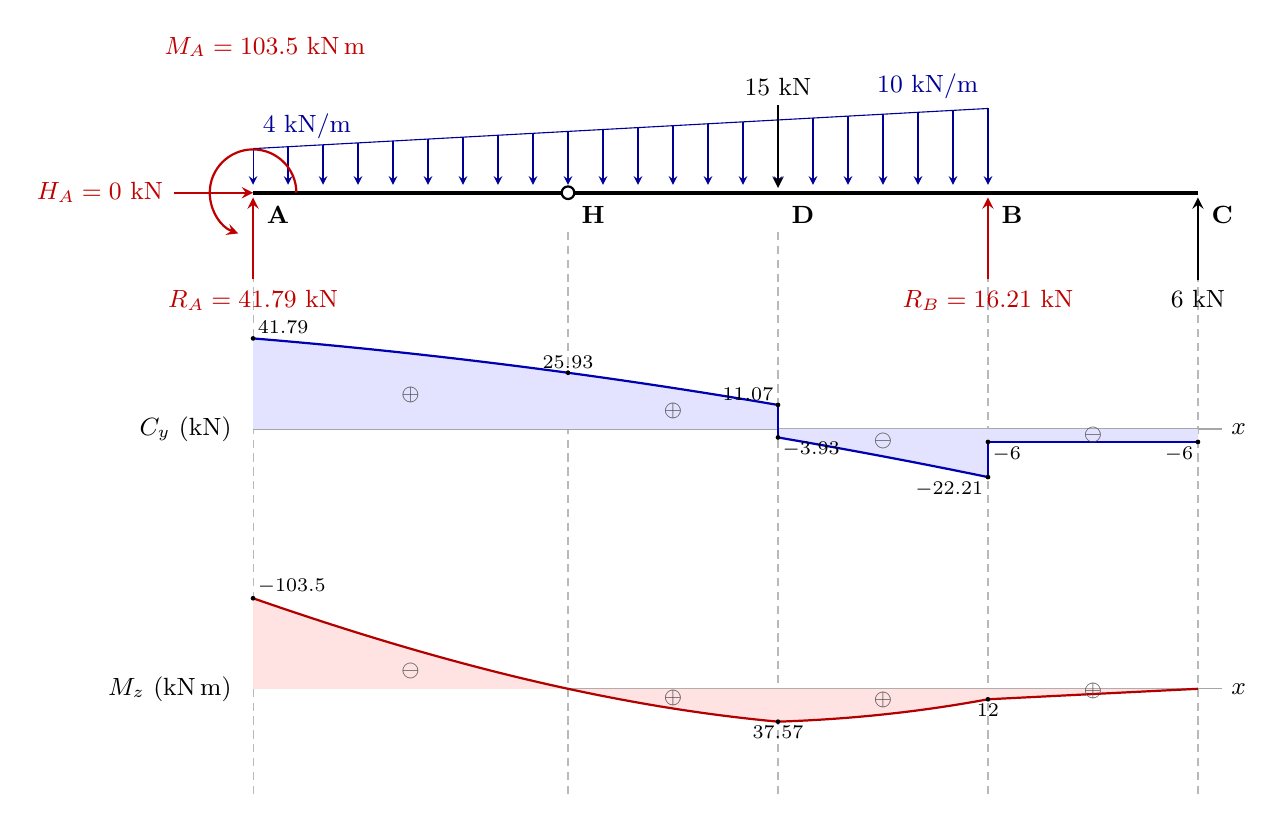
\begin{tikzpicture}
\draw[densely dashed,gray!55] (12.0000,-0.5000) -- (12.0000,-7.7000);
\draw[densely dashed,gray!55] (9.3333,-0.5000) -- (9.3333,-7.7000);
\draw[densely dashed,gray!55] (6.6667,-0.5000) -- (6.6667,-7.7000);
\draw[densely dashed,gray!55] (4.0000,-0.5000) -- (4.0000,-7.7000);
\draw[densely dashed,gray!55] (0.0000,-0.5000) -- (0.0000,-7.7000);
\draw[-stealth,blue!60!black] (0.0000,0.5600) -- (0.0000,0.1000);
\draw[-stealth,blue!60!black] (0.4444,0.5843) -- (0.4444,0.1000);
\draw[-stealth,blue!60!black] (0.8889,0.6086) -- (0.8889,0.1000);
\draw[-stealth,blue!60!black] (1.3333,0.6329) -- (1.3333,0.1000);
\draw[-stealth,blue!60!black] (1.7778,0.6571) -- (1.7778,0.1000);
\draw[-stealth,blue!60!black] (2.2222,0.6814) -- (2.2222,0.1000);
\draw[-stealth,blue!60!black] (2.6667,0.7057) -- (2.6667,0.1000);
\draw[-stealth,blue!60!black] (3.1111,0.7300) -- (3.1111,0.1000);
\draw[-stealth,blue!60!black] (3.5556,0.7543) -- (3.5556,0.1000);
\draw[-stealth,blue!60!black] (4.0000,0.7786) -- (4.0000,0.1000);
\draw[-stealth,blue!60!black] (4.4444,0.8029) -- (4.4444,0.1000);
\draw[-stealth,blue!60!black] (4.8889,0.8271) -- (4.8889,0.1000);
\draw[-stealth,blue!60!black] (5.3333,0.8514) -- (5.3333,0.1000);
\draw[-stealth,blue!60!black] (5.7778,0.8757) -- (5.7778,0.1000);
\draw[-stealth,blue!60!black] (6.2222,0.9000) -- (6.2222,0.1000);
\draw[-stealth,blue!60!black] (6.6667,0.9243) -- (6.6667,0.1000);
\draw[-stealth,blue!60!black] (7.1111,0.9486) -- (7.1111,0.1000);
\draw[-stealth,blue!60!black] (7.5556,0.9729) -- (7.5556,0.1000);
\draw[-stealth,blue!60!black] (8.0000,0.9971) -- (8.0000,0.1000);
\draw[-stealth,blue!60!black] (8.4444,1.0214) -- (8.4444,0.1000);
\draw[-stealth,blue!60!black] (8.8889,1.0457) -- (8.8889,0.1000);
\draw[-stealth,blue!60!black] (9.3333,1.0700) -- (9.3333,0.1000);
% studium:at distributed 0 x=0 to=7 check=span
\draw[blue!60!black] (0.0000,0.5600) -- (0.4444,0.5843) -- (0.8889,0.6086) -- (1.3333,0.6329) -- (1.7778,0.6571) -- (2.2222,0.6814) -- (2.6667,0.7057) -- (3.1111,0.7300) -- (3.5556,0.7543) -- (4.0000,0.7786) -- (4.4444,0.8029) -- (4.8889,0.8271) -- (5.3333,0.8514) -- (5.7778,0.8757) -- (6.2222,0.9000) -- (6.6667,0.9243) -- (7.1111,0.9486) -- (7.5556,0.9729) -- (8.0000,0.9971) -- (8.4444,1.0214) -- (8.8889,1.0457) -- (9.3333,1.0700);
\node[font=\small,anchor=south west,blue!60!black] at (0.0000,0.5600) {$4$~\mbox{kN/m}};
\node[font=\small,anchor=south east,blue!60!black] at (9.3333,1.0700) {$10$~\mbox{kN/m}};
\draw[line width=1.6pt] (0,0.0000) -- (12.0000,0.0000);
% studium:at hinge 0 x=3 check=first
\draw[thick,fill=white] (4.0000,0.0000) circle (0.08);
% studium:at force 0 x=5 check=tip
\draw[-stealth,thick,black] (6.6667,1.1100) -- (6.6667,0.0600);
\node[font=\small,anchor=south] at (6.6667,1.1100) {$15$~\mbox{kN}};
% studium:at force 1 x=9 check=tip
\draw[-stealth,thick,black] (12.0000,-1.1100) -- (12.0000,-0.0600);
\node[font=\small,anchor=north] at (12.0000,-1.1100) {$6$~\mbox{kN}};
% studium:reaction H_A value=0
% studium:at reaction H_A x=0 check=tip
\draw[-stealth,thick,red!75!black] (-1.0000,0.0000) -- (0.0000,0.0000);
\node[font=\small,anchor=east,red!75!black] at (-1.0200,0.0000) {$H_{A} = 0$~\mbox{kN}};
% studium:reaction R_A value=41.79
% studium:at reaction R_A x=0 check=tip
\draw[-stealth,thick,red!75!black] (0.0000,-1.1000) -- (0.0000,-0.0600);
\node[font=\small,anchor=north,red!75!black] at (0.0000,-1.1200) {$R_{A} = 41.79$~\mbox{kN}};
% studium:reaction M_A value=103.5
% studium:at reaction M_A x=0 check=arc
\draw[-stealth,thick,red!75!black] (0.5500,0.0000) arc (0:250:0.55);
\node[font=\small,anchor=south,red!75!black] at (0.1500,1.6000) {$M_{A} = 103.5$~\mbox{kN\,m}};
% studium:reaction R_B value=16.21
% studium:at reaction R_B x=7 check=tip
\draw[-stealth,thick,red!75!black] (9.3333,-1.1000) -- (9.3333,-0.0600);
\node[font=\small,anchor=north,red!75!black] at (9.3333,-1.1200) {$R_{B} = 16.21$~\mbox{kN}};
\node[font=\small\bfseries,anchor=north west] at (0.0500,-0.0500) {A};
\node[font=\small\bfseries,anchor=north west] at (4.0500,-0.0500) {H};
\node[font=\small\bfseries,anchor=north west] at (6.7167,-0.0500) {D};
\node[font=\small\bfseries,anchor=north west] at (9.3833,-0.0500) {B};
\node[font=\small\bfseries,anchor=north west] at (12.0500,-0.0500) {C};
\draw[gray!70] (0,-3.0000) -- (12.3000,-3.0000);
\fill[blue!11] (0.0000,-3.0000) -- (0.0000,-1.8500) -- (0.1250,-1.8604) -- (0.2500,-1.8711) -- (0.3750,-1.8819) -- (0.5000,-1.8929) -- (0.6250,-1.9042) -- (0.7500,-1.9157) -- (0.8750,-1.9273) -- (1.0000,-1.9392) -- (1.1250,-1.9513) -- (1.2500,-1.9636) -- (1.3750,-1.9761) -- (1.5000,-1.9888) -- (1.6250,-2.0017) -- (1.7500,-2.0148) -- (1.8750,-2.0281) -- (2.0000,-2.0417) -- (2.1250,-2.0554) -- (2.2500,-2.0694) -- (2.3750,-2.0835) -- (2.5000,-2.0979) -- (2.6250,-2.1124) -- (2.7500,-2.1272) -- (2.8750,-2.1422) -- (3.0000,-2.1574) -- (3.1250,-2.1728) -- (3.2500,-2.1884) -- (3.3750,-2.2042) -- (3.5000,-2.2202) -- (3.6250,-2.2365) -- (3.7500,-2.2529) -- (3.8750,-2.2696) -- (4.0000,-2.2864) -- (4.0000,-3.0000) -- cycle;
\fill[blue!11] (4.0000,-3.0000) -- (4.0000,-2.2864) -- (4.0833,-2.2978) -- (4.1667,-2.3092) -- (4.2500,-2.3207) -- (4.3333,-2.3324) -- (4.4167,-2.3441) -- (4.5000,-2.3559) -- (4.5833,-2.3678) -- (4.6667,-2.3798) -- (4.7500,-2.3919) -- (4.8333,-2.4041) -- (4.9167,-2.4163) -- (5.0000,-2.4287) -- (5.0833,-2.4411) -- (5.1667,-2.4537) -- (5.2500,-2.4663) -- (5.3333,-2.4791) -- (5.4167,-2.4919) -- (5.5000,-2.5048) -- (5.5833,-2.5178) -- (5.6667,-2.5309) -- (5.7500,-2.5441) -- (5.8333,-2.5574) -- (5.9167,-2.5708) -- (6.0000,-2.5842) -- (6.0833,-2.5978) -- (6.1667,-2.6114) -- (6.2500,-2.6252) -- (6.3333,-2.6390) -- (6.4167,-2.6530) -- (6.5000,-2.6670) -- (6.5833,-2.6811) -- (6.6667,-2.6953) -- (6.6667,-3.0000) -- cycle;
\fill[blue!11] (6.6667,-3.0000) -- (6.6667,-3.1081) -- (6.7500,-3.1224) -- (6.8333,-3.1368) -- (6.9167,-3.1513) -- (7.0000,-3.1659) -- (7.0833,-3.1805) -- (7.1667,-3.1953) -- (7.2500,-3.2101) -- (7.3333,-3.2251) -- (7.4167,-3.2401) -- (7.5000,-3.2552) -- (7.5833,-3.2705) -- (7.6667,-3.2858) -- (7.7500,-3.3012) -- (7.8333,-3.3167) -- (7.9167,-3.3323) -- (8.0000,-3.3479) -- (8.0833,-3.3637) -- (8.1667,-3.3796) -- (8.2500,-3.3955) -- (8.3333,-3.4116) -- (8.4167,-3.4277) -- (8.5000,-3.4440) -- (8.5833,-3.4603) -- (8.6667,-3.4767) -- (8.7500,-3.4932) -- (8.8333,-3.5098) -- (8.9167,-3.5265) -- (9.0000,-3.5433) -- (9.0833,-3.5602) -- (9.1667,-3.5772) -- (9.2500,-3.5942) -- (9.3333,-3.6114) -- (9.3333,-3.0000) -- cycle;
\fill[blue!11] (9.3333,-3.0000) -- (9.3333,-3.1651) -- (12.0000,-3.1651) -- (12.0000,-3.0000) -- cycle;
% studium:series V sx=1.3333333333333333 sy=0.02752136752136752 x0=0.0 y0=-3.0 sign=1
\draw[thick,blue!70!black] (0.0000,-1.8500) -- (0.1250,-1.8604) -- (0.2500,-1.8711) -- (0.3750,-1.8819) -- (0.5000,-1.8929) -- (0.6250,-1.9042) -- (0.7500,-1.9157) -- (0.8750,-1.9273) -- (1.0000,-1.9392) -- (1.1250,-1.9513) -- (1.2500,-1.9636) -- (1.3750,-1.9761) -- (1.5000,-1.9888) -- (1.6250,-2.0017) -- (1.7500,-2.0148) -- (1.8750,-2.0281) -- (2.0000,-2.0417) -- (2.1250,-2.0554) -- (2.2500,-2.0694) -- (2.3750,-2.0835) -- (2.5000,-2.0979) -- (2.6250,-2.1124) -- (2.7500,-2.1272) -- (2.8750,-2.1422) -- (3.0000,-2.1574) -- (3.1250,-2.1728) -- (3.2500,-2.1884) -- (3.3750,-2.2042) -- (3.5000,-2.2202) -- (3.6250,-2.2365) -- (3.7500,-2.2529) -- (3.8750,-2.2696) -- (4.0000,-2.2864);
\draw[thick,blue!70!black] (4.0000,-2.2864) -- (4.0833,-2.2978) -- (4.1667,-2.3092) -- (4.2500,-2.3207) -- (4.3333,-2.3324) -- (4.4167,-2.3441) -- (4.5000,-2.3559) -- (4.5833,-2.3678) -- (4.6667,-2.3798) -- (4.7500,-2.3919) -- (4.8333,-2.4041) -- (4.9167,-2.4163) -- (5.0000,-2.4287) -- (5.0833,-2.4411) -- (5.1667,-2.4537) -- (5.2500,-2.4663) -- (5.3333,-2.4791) -- (5.4167,-2.4919) -- (5.5000,-2.5048) -- (5.5833,-2.5178) -- (5.6667,-2.5309) -- (5.7500,-2.5441) -- (5.8333,-2.5574) -- (5.9167,-2.5708) -- (6.0000,-2.5842) -- (6.0833,-2.5978) -- (6.1667,-2.6114) -- (6.2500,-2.6252) -- (6.3333,-2.6390) -- (6.4167,-2.6530) -- (6.5000,-2.6670) -- (6.5833,-2.6811) -- (6.6667,-2.6953);
\draw[thick,blue!70!black] (6.6667,-3.1081) -- (6.7500,-3.1224) -- (6.8333,-3.1368) -- (6.9167,-3.1513) -- (7.0000,-3.1659) -- (7.0833,-3.1805) -- (7.1667,-3.1953) -- (7.2500,-3.2101) -- (7.3333,-3.2251) -- (7.4167,-3.2401) -- (7.5000,-3.2552) -- (7.5833,-3.2705) -- (7.6667,-3.2858) -- (7.7500,-3.3012) -- (7.8333,-3.3167) -- (7.9167,-3.3323) -- (8.0000,-3.3479) -- (8.0833,-3.3637) -- (8.1667,-3.3796) -- (8.2500,-3.3955) -- (8.3333,-3.4116) -- (8.4167,-3.4277) -- (8.5000,-3.4440) -- (8.5833,-3.4603) -- (8.6667,-3.4767) -- (8.7500,-3.4932) -- (8.8333,-3.5098) -- (8.9167,-3.5265) -- (9.0000,-3.5433) -- (9.0833,-3.5602) -- (9.1667,-3.5772) -- (9.2500,-3.5942) -- (9.3333,-3.6114);
\draw[thick,blue!70!black] (9.3333,-3.1651) -- (12.0000,-3.1651);
% studium:end V
\draw[thick,blue!70!black] (6.6667,-2.6953) -- (6.6667,-3.1081);
\draw[thick,blue!70!black] (9.3333,-3.6114) -- (9.3333,-3.1651);
\node[font=\small,anchor=east] at (-0.15,-3.0000) {$C_y$ (kN)};
\node[font=\small,anchor=west] at (12.3000,-3.0000) {$x$};
% studium:label V x=0 side=right value=41.79
\fill (0.0000,-1.8500) circle (0.03);
\node[font=\scriptsize,anchor=south west,inner sep=1.5pt] at (0.0000,-1.8500) {$41.79$};
% studium:label V x=3 side=both value=25.93
\fill (4.0000,-2.2864) circle (0.03);
\node[font=\scriptsize,anchor=south,inner sep=1.5pt] at (4.0000,-2.2864) {$25.93$};
% studium:label V x=5 side=left value=11.07
\fill (6.6667,-2.6953) circle (0.03);
\node[font=\scriptsize,anchor=south east,inner sep=1.5pt] at (6.6667,-2.6953) {$11.07$};
% studium:label V x=5 side=right value=-3.93
\fill (6.6667,-3.1081) circle (0.03);
\node[font=\scriptsize,anchor=north west,inner sep=1.5pt] at (6.6667,-3.1081) {$-3.93$};
% studium:label V x=7 side=left value=-22.21
\fill (9.3333,-3.6114) circle (0.03);
\node[font=\scriptsize,anchor=north east,inner sep=1.5pt] at (9.3333,-3.6114) {$-22.21$};
% studium:label V x=7 side=right value=-6
\fill (9.3333,-3.1651) circle (0.03);
\node[font=\scriptsize,anchor=north west,inner sep=1.5pt] at (9.3333,-3.1651) {$-6$};
% studium:label V x=9 side=left value=-6
\fill (12.0000,-3.1651) circle (0.03);
\node[font=\scriptsize,anchor=north east,inner sep=1.5pt] at (12.0000,-3.1651) {$-6$};
\node[font=\footnotesize,gray!60!black] at (2.0000,-2.5688) {$\oplus$};
\node[font=\footnotesize,gray!60!black] at (5.3333,-2.7656) {$\oplus$};
\node[font=\footnotesize,gray!60!black] at (8.0000,-3.1566) {$\ominus$};
\node[font=\footnotesize,gray!60!black] at (10.6667,-3.0743) {$\ominus$};
\draw[gray!70] (0,-6.3000) -- (12.3000,-6.3000);
\fill[red!11] (0.0000,-6.3000) -- (0.0000,-5.1500) -- (0.1250,-5.1933) -- (0.2500,-5.2363) -- (0.3750,-5.2788) -- (0.5000,-5.3209) -- (0.6250,-5.3626) -- (0.7500,-5.4038) -- (0.8750,-5.4447) -- (1.0000,-5.4850) -- (1.1250,-5.5250) -- (1.2500,-5.5644) -- (1.3750,-5.6034) -- (1.5000,-5.6419) -- (1.6250,-5.6800) -- (1.7500,-5.7175) -- (1.8750,-5.7545) -- (2.0000,-5.7911) -- (2.1250,-5.8271) -- (2.2500,-5.8626) -- (2.3750,-5.8975) -- (2.5000,-5.9319) -- (2.6250,-5.9658) -- (2.7500,-5.9991) -- (2.8750,-6.0319) -- (3.0000,-6.0641) -- (3.1250,-6.0957) -- (3.2500,-6.1267) -- (3.3750,-6.1571) -- (3.5000,-6.1869) -- (3.6250,-6.2161) -- (3.7500,-6.2447) -- (3.8750,-6.2727) -- (4.0000,-6.3000) -- (4.0000,-6.3000) -- cycle;
\fill[red!11] (4.0000,-6.3000) -- (4.0000,-6.3000) -- (4.0833,-6.3179) -- (4.1667,-6.3354) -- (4.2500,-6.3527) -- (4.3333,-6.3697) -- (4.4167,-6.3864) -- (4.5000,-6.4028) -- (4.5833,-6.4189) -- (4.6667,-6.4347) -- (4.7500,-6.4502) -- (4.8333,-6.4654) -- (4.9167,-6.4803) -- (5.0000,-6.4949) -- (5.0833,-6.5091) -- (5.1667,-6.5231) -- (5.2500,-6.5367) -- (5.3333,-6.5500) -- (5.4167,-6.5630) -- (5.5000,-6.5756) -- (5.5833,-6.5880) -- (5.6667,-6.6000) -- (5.7500,-6.6116) -- (5.8333,-6.6230) -- (5.9167,-6.6340) -- (6.0000,-6.6446) -- (6.0833,-6.6550) -- (6.1667,-6.6649) -- (6.2500,-6.6746) -- (6.3333,-6.6839) -- (6.4167,-6.6928) -- (6.5000,-6.7014) -- (6.5833,-6.7096) -- (6.6667,-6.7175) -- (6.6667,-6.3000) -- cycle;
\fill[red!11] (6.6667,-6.3000) -- (6.6667,-6.7175) -- (6.7500,-6.7146) -- (6.8333,-6.7113) -- (6.9167,-6.7076) -- (7.0000,-6.7036) -- (7.0833,-6.6993) -- (7.1667,-6.6945) -- (7.2500,-6.6894) -- (7.3333,-6.6839) -- (7.4167,-6.6781) -- (7.5000,-6.6718) -- (7.5833,-6.6652) -- (7.6667,-6.6582) -- (7.7500,-6.6508) -- (7.8333,-6.6430) -- (7.9167,-6.6348) -- (8.0000,-6.6262) -- (8.0833,-6.6172) -- (8.1667,-6.6078) -- (8.2500,-6.5981) -- (8.3333,-6.5879) -- (8.4167,-6.5773) -- (8.5000,-6.5663) -- (8.5833,-6.5549) -- (8.6667,-6.5431) -- (8.7500,-6.5308) -- (8.8333,-6.5182) -- (8.9167,-6.5051) -- (9.0000,-6.4916) -- (9.0833,-6.4777) -- (9.1667,-6.4633) -- (9.2500,-6.4485) -- (9.3333,-6.4333) -- (9.3333,-6.3000) -- cycle;
\fill[red!11] (9.3333,-6.3000) -- (9.3333,-6.4333) -- (12.0000,-6.3000) -- (12.0000,-6.3000) -- cycle;
% studium:series M sx=1.3333333333333333 sy=0.01111111111111111 x0=0.0 y0=-6.3 sign=-1
\draw[thick,red!70!black] (0.0000,-5.1500) -- (0.1250,-5.1933) -- (0.2500,-5.2363) -- (0.3750,-5.2788) -- (0.5000,-5.3209) -- (0.6250,-5.3626) -- (0.7500,-5.4038) -- (0.8750,-5.4447) -- (1.0000,-5.4850) -- (1.1250,-5.5250) -- (1.2500,-5.5644) -- (1.3750,-5.6034) -- (1.5000,-5.6419) -- (1.6250,-5.6800) -- (1.7500,-5.7175) -- (1.8750,-5.7545) -- (2.0000,-5.7911) -- (2.1250,-5.8271) -- (2.2500,-5.8626) -- (2.3750,-5.8975) -- (2.5000,-5.9319) -- (2.6250,-5.9658) -- (2.7500,-5.9991) -- (2.8750,-6.0319) -- (3.0000,-6.0641) -- (3.1250,-6.0957) -- (3.2500,-6.1267) -- (3.3750,-6.1571) -- (3.5000,-6.1869) -- (3.6250,-6.2161) -- (3.7500,-6.2447) -- (3.8750,-6.2727) -- (4.0000,-6.3000);
\draw[thick,red!70!black] (4.0000,-6.3000) -- (4.0833,-6.3179) -- (4.1667,-6.3354) -- (4.2500,-6.3527) -- (4.3333,-6.3697) -- (4.4167,-6.3864) -- (4.5000,-6.4028) -- (4.5833,-6.4189) -- (4.6667,-6.4347) -- (4.7500,-6.4502) -- (4.8333,-6.4654) -- (4.9167,-6.4803) -- (5.0000,-6.4949) -- (5.0833,-6.5091) -- (5.1667,-6.5231) -- (5.2500,-6.5367) -- (5.3333,-6.5500) -- (5.4167,-6.5630) -- (5.5000,-6.5756) -- (5.5833,-6.5880) -- (5.6667,-6.6000) -- (5.7500,-6.6116) -- (5.8333,-6.6230) -- (5.9167,-6.6340) -- (6.0000,-6.6446) -- (6.0833,-6.6550) -- (6.1667,-6.6649) -- (6.2500,-6.6746) -- (6.3333,-6.6839) -- (6.4167,-6.6928) -- (6.5000,-6.7014) -- (6.5833,-6.7096) -- (6.6667,-6.7175);
\draw[thick,red!70!black] (6.6667,-6.7175) -- (6.7500,-6.7146) -- (6.8333,-6.7113) -- (6.9167,-6.7076) -- (7.0000,-6.7036) -- (7.0833,-6.6993) -- (7.1667,-6.6945) -- (7.2500,-6.6894) -- (7.3333,-6.6839) -- (7.4167,-6.6781) -- (7.5000,-6.6718) -- (7.5833,-6.6652) -- (7.6667,-6.6582) -- (7.7500,-6.6508) -- (7.8333,-6.6430) -- (7.9167,-6.6348) -- (8.0000,-6.6262) -- (8.0833,-6.6172) -- (8.1667,-6.6078) -- (8.2500,-6.5981) -- (8.3333,-6.5879) -- (8.4167,-6.5773) -- (8.5000,-6.5663) -- (8.5833,-6.5549) -- (8.6667,-6.5431) -- (8.7500,-6.5308) -- (8.8333,-6.5182) -- (8.9167,-6.5051) -- (9.0000,-6.4916) -- (9.0833,-6.4777) -- (9.1667,-6.4633) -- (9.2500,-6.4485) -- (9.3333,-6.4333);
\draw[thick,red!70!black] (9.3333,-6.4333) -- (12.0000,-6.3000);
% studium:end M
\node[font=\small,anchor=east] at (-0.15,-6.3000) {$M_z$ (kN\,m)};
\node[font=\small,anchor=west] at (12.3000,-6.3000) {$x$};
% studium:label M x=0 side=right value=-103.5
\fill (0.0000,-5.1500) circle (0.03);
\node[font=\scriptsize,anchor=south west,inner sep=1.5pt] at (0.0000,-5.1500) {$-103.5$};
% studium:label M x=5 side=both value=37.57
\fill (6.6667,-6.7175) circle (0.03);
\node[font=\scriptsize,anchor=north,inner sep=1.5pt] at (6.6667,-6.7175) {$37.57$};
% studium:label M x=7 side=both value=12
\fill (9.3333,-6.4333) circle (0.03);
\node[font=\scriptsize,anchor=north,inner sep=1.5pt] at (9.3333,-6.4333) {$12$};
\node[font=\footnotesize,gray!60!black] at (2.0000,-6.0710) {$\ominus$};
\node[font=\footnotesize,gray!60!black] at (5.3333,-6.4125) {$\oplus$};
\node[font=\footnotesize,gray!60!black] at (8.0000,-6.4468) {$\oplus$};
\node[font=\footnotesize,gray!60!black] at (10.6667,-6.3300) {$\oplus$};
\end{tikzpicture}}%
\else
\ifnum\count0>\count4
\resizebox{!}{\dimexpr\textheight/100*38\relax}{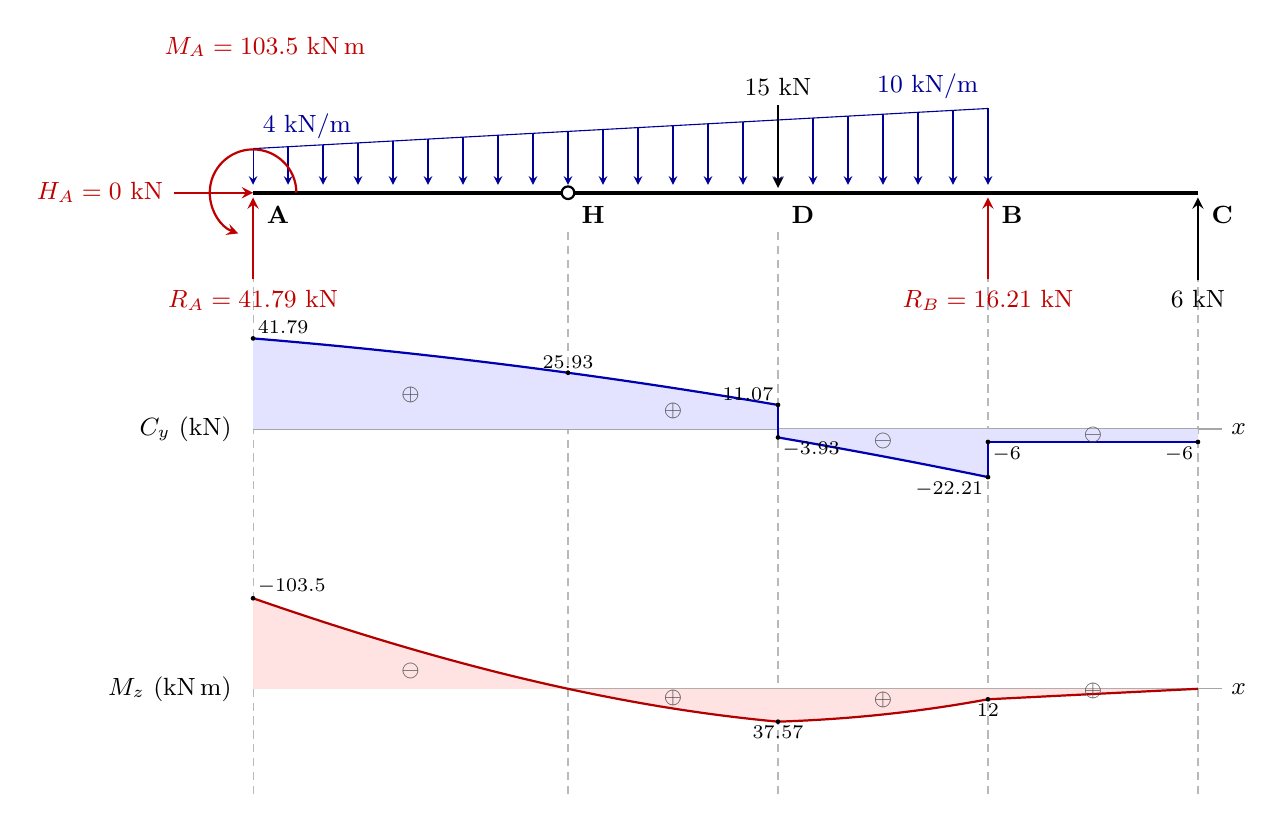
\begin{tikzpicture}
\draw[densely dashed,gray!55] (12.0000,-0.5000) -- (12.0000,-7.7000);
\draw[densely dashed,gray!55] (9.3333,-0.5000) -- (9.3333,-7.7000);
\draw[densely dashed,gray!55] (6.6667,-0.5000) -- (6.6667,-7.7000);
\draw[densely dashed,gray!55] (4.0000,-0.5000) -- (4.0000,-7.7000);
\draw[densely dashed,gray!55] (0.0000,-0.5000) -- (0.0000,-7.7000);
\draw[-stealth,blue!60!black] (0.0000,0.5600) -- (0.0000,0.1000);
\draw[-stealth,blue!60!black] (0.4444,0.5843) -- (0.4444,0.1000);
\draw[-stealth,blue!60!black] (0.8889,0.6086) -- (0.8889,0.1000);
\draw[-stealth,blue!60!black] (1.3333,0.6329) -- (1.3333,0.1000);
\draw[-stealth,blue!60!black] (1.7778,0.6571) -- (1.7778,0.1000);
\draw[-stealth,blue!60!black] (2.2222,0.6814) -- (2.2222,0.1000);
\draw[-stealth,blue!60!black] (2.6667,0.7057) -- (2.6667,0.1000);
\draw[-stealth,blue!60!black] (3.1111,0.7300) -- (3.1111,0.1000);
\draw[-stealth,blue!60!black] (3.5556,0.7543) -- (3.5556,0.1000);
\draw[-stealth,blue!60!black] (4.0000,0.7786) -- (4.0000,0.1000);
\draw[-stealth,blue!60!black] (4.4444,0.8029) -- (4.4444,0.1000);
\draw[-stealth,blue!60!black] (4.8889,0.8271) -- (4.8889,0.1000);
\draw[-stealth,blue!60!black] (5.3333,0.8514) -- (5.3333,0.1000);
\draw[-stealth,blue!60!black] (5.7778,0.8757) -- (5.7778,0.1000);
\draw[-stealth,blue!60!black] (6.2222,0.9000) -- (6.2222,0.1000);
\draw[-stealth,blue!60!black] (6.6667,0.9243) -- (6.6667,0.1000);
\draw[-stealth,blue!60!black] (7.1111,0.9486) -- (7.1111,0.1000);
\draw[-stealth,blue!60!black] (7.5556,0.9729) -- (7.5556,0.1000);
\draw[-stealth,blue!60!black] (8.0000,0.9971) -- (8.0000,0.1000);
\draw[-stealth,blue!60!black] (8.4444,1.0214) -- (8.4444,0.1000);
\draw[-stealth,blue!60!black] (8.8889,1.0457) -- (8.8889,0.1000);
\draw[-stealth,blue!60!black] (9.3333,1.0700) -- (9.3333,0.1000);
% studium:at distributed 0 x=0 to=7 check=span
\draw[blue!60!black] (0.0000,0.5600) -- (0.4444,0.5843) -- (0.8889,0.6086) -- (1.3333,0.6329) -- (1.7778,0.6571) -- (2.2222,0.6814) -- (2.6667,0.7057) -- (3.1111,0.7300) -- (3.5556,0.7543) -- (4.0000,0.7786) -- (4.4444,0.8029) -- (4.8889,0.8271) -- (5.3333,0.8514) -- (5.7778,0.8757) -- (6.2222,0.9000) -- (6.6667,0.9243) -- (7.1111,0.9486) -- (7.5556,0.9729) -- (8.0000,0.9971) -- (8.4444,1.0214) -- (8.8889,1.0457) -- (9.3333,1.0700);
\node[font=\small,anchor=south west,blue!60!black] at (0.0000,0.5600) {$4$~\mbox{kN/m}};
\node[font=\small,anchor=south east,blue!60!black] at (9.3333,1.0700) {$10$~\mbox{kN/m}};
\draw[line width=1.6pt] (0,0.0000) -- (12.0000,0.0000);
% studium:at hinge 0 x=3 check=first
\draw[thick,fill=white] (4.0000,0.0000) circle (0.08);
% studium:at force 0 x=5 check=tip
\draw[-stealth,thick,black] (6.6667,1.1100) -- (6.6667,0.0600);
\node[font=\small,anchor=south] at (6.6667,1.1100) {$15$~\mbox{kN}};
% studium:at force 1 x=9 check=tip
\draw[-stealth,thick,black] (12.0000,-1.1100) -- (12.0000,-0.0600);
\node[font=\small,anchor=north] at (12.0000,-1.1100) {$6$~\mbox{kN}};
% studium:reaction H_A value=0
% studium:at reaction H_A x=0 check=tip
\draw[-stealth,thick,red!75!black] (-1.0000,0.0000) -- (0.0000,0.0000);
\node[font=\small,anchor=east,red!75!black] at (-1.0200,0.0000) {$H_{A} = 0$~\mbox{kN}};
% studium:reaction R_A value=41.79
% studium:at reaction R_A x=0 check=tip
\draw[-stealth,thick,red!75!black] (0.0000,-1.1000) -- (0.0000,-0.0600);
\node[font=\small,anchor=north,red!75!black] at (0.0000,-1.1200) {$R_{A} = 41.79$~\mbox{kN}};
% studium:reaction M_A value=103.5
% studium:at reaction M_A x=0 check=arc
\draw[-stealth,thick,red!75!black] (0.5500,0.0000) arc (0:250:0.55);
\node[font=\small,anchor=south,red!75!black] at (0.1500,1.6000) {$M_{A} = 103.5$~\mbox{kN\,m}};
% studium:reaction R_B value=16.21
% studium:at reaction R_B x=7 check=tip
\draw[-stealth,thick,red!75!black] (9.3333,-1.1000) -- (9.3333,-0.0600);
\node[font=\small,anchor=north,red!75!black] at (9.3333,-1.1200) {$R_{B} = 16.21$~\mbox{kN}};
\node[font=\small\bfseries,anchor=north west] at (0.0500,-0.0500) {A};
\node[font=\small\bfseries,anchor=north west] at (4.0500,-0.0500) {H};
\node[font=\small\bfseries,anchor=north west] at (6.7167,-0.0500) {D};
\node[font=\small\bfseries,anchor=north west] at (9.3833,-0.0500) {B};
\node[font=\small\bfseries,anchor=north west] at (12.0500,-0.0500) {C};
\draw[gray!70] (0,-3.0000) -- (12.3000,-3.0000);
\fill[blue!11] (0.0000,-3.0000) -- (0.0000,-1.8500) -- (0.1250,-1.8604) -- (0.2500,-1.8711) -- (0.3750,-1.8819) -- (0.5000,-1.8929) -- (0.6250,-1.9042) -- (0.7500,-1.9157) -- (0.8750,-1.9273) -- (1.0000,-1.9392) -- (1.1250,-1.9513) -- (1.2500,-1.9636) -- (1.3750,-1.9761) -- (1.5000,-1.9888) -- (1.6250,-2.0017) -- (1.7500,-2.0148) -- (1.8750,-2.0281) -- (2.0000,-2.0417) -- (2.1250,-2.0554) -- (2.2500,-2.0694) -- (2.3750,-2.0835) -- (2.5000,-2.0979) -- (2.6250,-2.1124) -- (2.7500,-2.1272) -- (2.8750,-2.1422) -- (3.0000,-2.1574) -- (3.1250,-2.1728) -- (3.2500,-2.1884) -- (3.3750,-2.2042) -- (3.5000,-2.2202) -- (3.6250,-2.2365) -- (3.7500,-2.2529) -- (3.8750,-2.2696) -- (4.0000,-2.2864) -- (4.0000,-3.0000) -- cycle;
\fill[blue!11] (4.0000,-3.0000) -- (4.0000,-2.2864) -- (4.0833,-2.2978) -- (4.1667,-2.3092) -- (4.2500,-2.3207) -- (4.3333,-2.3324) -- (4.4167,-2.3441) -- (4.5000,-2.3559) -- (4.5833,-2.3678) -- (4.6667,-2.3798) -- (4.7500,-2.3919) -- (4.8333,-2.4041) -- (4.9167,-2.4163) -- (5.0000,-2.4287) -- (5.0833,-2.4411) -- (5.1667,-2.4537) -- (5.2500,-2.4663) -- (5.3333,-2.4791) -- (5.4167,-2.4919) -- (5.5000,-2.5048) -- (5.5833,-2.5178) -- (5.6667,-2.5309) -- (5.7500,-2.5441) -- (5.8333,-2.5574) -- (5.9167,-2.5708) -- (6.0000,-2.5842) -- (6.0833,-2.5978) -- (6.1667,-2.6114) -- (6.2500,-2.6252) -- (6.3333,-2.6390) -- (6.4167,-2.6530) -- (6.5000,-2.6670) -- (6.5833,-2.6811) -- (6.6667,-2.6953) -- (6.6667,-3.0000) -- cycle;
\fill[blue!11] (6.6667,-3.0000) -- (6.6667,-3.1081) -- (6.7500,-3.1224) -- (6.8333,-3.1368) -- (6.9167,-3.1513) -- (7.0000,-3.1659) -- (7.0833,-3.1805) -- (7.1667,-3.1953) -- (7.2500,-3.2101) -- (7.3333,-3.2251) -- (7.4167,-3.2401) -- (7.5000,-3.2552) -- (7.5833,-3.2705) -- (7.6667,-3.2858) -- (7.7500,-3.3012) -- (7.8333,-3.3167) -- (7.9167,-3.3323) -- (8.0000,-3.3479) -- (8.0833,-3.3637) -- (8.1667,-3.3796) -- (8.2500,-3.3955) -- (8.3333,-3.4116) -- (8.4167,-3.4277) -- (8.5000,-3.4440) -- (8.5833,-3.4603) -- (8.6667,-3.4767) -- (8.7500,-3.4932) -- (8.8333,-3.5098) -- (8.9167,-3.5265) -- (9.0000,-3.5433) -- (9.0833,-3.5602) -- (9.1667,-3.5772) -- (9.2500,-3.5942) -- (9.3333,-3.6114) -- (9.3333,-3.0000) -- cycle;
\fill[blue!11] (9.3333,-3.0000) -- (9.3333,-3.1651) -- (12.0000,-3.1651) -- (12.0000,-3.0000) -- cycle;
% studium:series V sx=1.3333333333333333 sy=0.02752136752136752 x0=0.0 y0=-3.0 sign=1
\draw[thick,blue!70!black] (0.0000,-1.8500) -- (0.1250,-1.8604) -- (0.2500,-1.8711) -- (0.3750,-1.8819) -- (0.5000,-1.8929) -- (0.6250,-1.9042) -- (0.7500,-1.9157) -- (0.8750,-1.9273) -- (1.0000,-1.9392) -- (1.1250,-1.9513) -- (1.2500,-1.9636) -- (1.3750,-1.9761) -- (1.5000,-1.9888) -- (1.6250,-2.0017) -- (1.7500,-2.0148) -- (1.8750,-2.0281) -- (2.0000,-2.0417) -- (2.1250,-2.0554) -- (2.2500,-2.0694) -- (2.3750,-2.0835) -- (2.5000,-2.0979) -- (2.6250,-2.1124) -- (2.7500,-2.1272) -- (2.8750,-2.1422) -- (3.0000,-2.1574) -- (3.1250,-2.1728) -- (3.2500,-2.1884) -- (3.3750,-2.2042) -- (3.5000,-2.2202) -- (3.6250,-2.2365) -- (3.7500,-2.2529) -- (3.8750,-2.2696) -- (4.0000,-2.2864);
\draw[thick,blue!70!black] (4.0000,-2.2864) -- (4.0833,-2.2978) -- (4.1667,-2.3092) -- (4.2500,-2.3207) -- (4.3333,-2.3324) -- (4.4167,-2.3441) -- (4.5000,-2.3559) -- (4.5833,-2.3678) -- (4.6667,-2.3798) -- (4.7500,-2.3919) -- (4.8333,-2.4041) -- (4.9167,-2.4163) -- (5.0000,-2.4287) -- (5.0833,-2.4411) -- (5.1667,-2.4537) -- (5.2500,-2.4663) -- (5.3333,-2.4791) -- (5.4167,-2.4919) -- (5.5000,-2.5048) -- (5.5833,-2.5178) -- (5.6667,-2.5309) -- (5.7500,-2.5441) -- (5.8333,-2.5574) -- (5.9167,-2.5708) -- (6.0000,-2.5842) -- (6.0833,-2.5978) -- (6.1667,-2.6114) -- (6.2500,-2.6252) -- (6.3333,-2.6390) -- (6.4167,-2.6530) -- (6.5000,-2.6670) -- (6.5833,-2.6811) -- (6.6667,-2.6953);
\draw[thick,blue!70!black] (6.6667,-3.1081) -- (6.7500,-3.1224) -- (6.8333,-3.1368) -- (6.9167,-3.1513) -- (7.0000,-3.1659) -- (7.0833,-3.1805) -- (7.1667,-3.1953) -- (7.2500,-3.2101) -- (7.3333,-3.2251) -- (7.4167,-3.2401) -- (7.5000,-3.2552) -- (7.5833,-3.2705) -- (7.6667,-3.2858) -- (7.7500,-3.3012) -- (7.8333,-3.3167) -- (7.9167,-3.3323) -- (8.0000,-3.3479) -- (8.0833,-3.3637) -- (8.1667,-3.3796) -- (8.2500,-3.3955) -- (8.3333,-3.4116) -- (8.4167,-3.4277) -- (8.5000,-3.4440) -- (8.5833,-3.4603) -- (8.6667,-3.4767) -- (8.7500,-3.4932) -- (8.8333,-3.5098) -- (8.9167,-3.5265) -- (9.0000,-3.5433) -- (9.0833,-3.5602) -- (9.1667,-3.5772) -- (9.2500,-3.5942) -- (9.3333,-3.6114);
\draw[thick,blue!70!black] (9.3333,-3.1651) -- (12.0000,-3.1651);
% studium:end V
\draw[thick,blue!70!black] (6.6667,-2.6953) -- (6.6667,-3.1081);
\draw[thick,blue!70!black] (9.3333,-3.6114) -- (9.3333,-3.1651);
\node[font=\small,anchor=east] at (-0.15,-3.0000) {$C_y$ (kN)};
\node[font=\small,anchor=west] at (12.3000,-3.0000) {$x$};
% studium:label V x=0 side=right value=41.79
\fill (0.0000,-1.8500) circle (0.03);
\node[font=\scriptsize,anchor=south west,inner sep=1.5pt] at (0.0000,-1.8500) {$41.79$};
% studium:label V x=3 side=both value=25.93
\fill (4.0000,-2.2864) circle (0.03);
\node[font=\scriptsize,anchor=south,inner sep=1.5pt] at (4.0000,-2.2864) {$25.93$};
% studium:label V x=5 side=left value=11.07
\fill (6.6667,-2.6953) circle (0.03);
\node[font=\scriptsize,anchor=south east,inner sep=1.5pt] at (6.6667,-2.6953) {$11.07$};
% studium:label V x=5 side=right value=-3.93
\fill (6.6667,-3.1081) circle (0.03);
\node[font=\scriptsize,anchor=north west,inner sep=1.5pt] at (6.6667,-3.1081) {$-3.93$};
% studium:label V x=7 side=left value=-22.21
\fill (9.3333,-3.6114) circle (0.03);
\node[font=\scriptsize,anchor=north east,inner sep=1.5pt] at (9.3333,-3.6114) {$-22.21$};
% studium:label V x=7 side=right value=-6
\fill (9.3333,-3.1651) circle (0.03);
\node[font=\scriptsize,anchor=north west,inner sep=1.5pt] at (9.3333,-3.1651) {$-6$};
% studium:label V x=9 side=left value=-6
\fill (12.0000,-3.1651) circle (0.03);
\node[font=\scriptsize,anchor=north east,inner sep=1.5pt] at (12.0000,-3.1651) {$-6$};
\node[font=\footnotesize,gray!60!black] at (2.0000,-2.5688) {$\oplus$};
\node[font=\footnotesize,gray!60!black] at (5.3333,-2.7656) {$\oplus$};
\node[font=\footnotesize,gray!60!black] at (8.0000,-3.1566) {$\ominus$};
\node[font=\footnotesize,gray!60!black] at (10.6667,-3.0743) {$\ominus$};
\draw[gray!70] (0,-6.3000) -- (12.3000,-6.3000);
\fill[red!11] (0.0000,-6.3000) -- (0.0000,-5.1500) -- (0.1250,-5.1933) -- (0.2500,-5.2363) -- (0.3750,-5.2788) -- (0.5000,-5.3209) -- (0.6250,-5.3626) -- (0.7500,-5.4038) -- (0.8750,-5.4447) -- (1.0000,-5.4850) -- (1.1250,-5.5250) -- (1.2500,-5.5644) -- (1.3750,-5.6034) -- (1.5000,-5.6419) -- (1.6250,-5.6800) -- (1.7500,-5.7175) -- (1.8750,-5.7545) -- (2.0000,-5.7911) -- (2.1250,-5.8271) -- (2.2500,-5.8626) -- (2.3750,-5.8975) -- (2.5000,-5.9319) -- (2.6250,-5.9658) -- (2.7500,-5.9991) -- (2.8750,-6.0319) -- (3.0000,-6.0641) -- (3.1250,-6.0957) -- (3.2500,-6.1267) -- (3.3750,-6.1571) -- (3.5000,-6.1869) -- (3.6250,-6.2161) -- (3.7500,-6.2447) -- (3.8750,-6.2727) -- (4.0000,-6.3000) -- (4.0000,-6.3000) -- cycle;
\fill[red!11] (4.0000,-6.3000) -- (4.0000,-6.3000) -- (4.0833,-6.3179) -- (4.1667,-6.3354) -- (4.2500,-6.3527) -- (4.3333,-6.3697) -- (4.4167,-6.3864) -- (4.5000,-6.4028) -- (4.5833,-6.4189) -- (4.6667,-6.4347) -- (4.7500,-6.4502) -- (4.8333,-6.4654) -- (4.9167,-6.4803) -- (5.0000,-6.4949) -- (5.0833,-6.5091) -- (5.1667,-6.5231) -- (5.2500,-6.5367) -- (5.3333,-6.5500) -- (5.4167,-6.5630) -- (5.5000,-6.5756) -- (5.5833,-6.5880) -- (5.6667,-6.6000) -- (5.7500,-6.6116) -- (5.8333,-6.6230) -- (5.9167,-6.6340) -- (6.0000,-6.6446) -- (6.0833,-6.6550) -- (6.1667,-6.6649) -- (6.2500,-6.6746) -- (6.3333,-6.6839) -- (6.4167,-6.6928) -- (6.5000,-6.7014) -- (6.5833,-6.7096) -- (6.6667,-6.7175) -- (6.6667,-6.3000) -- cycle;
\fill[red!11] (6.6667,-6.3000) -- (6.6667,-6.7175) -- (6.7500,-6.7146) -- (6.8333,-6.7113) -- (6.9167,-6.7076) -- (7.0000,-6.7036) -- (7.0833,-6.6993) -- (7.1667,-6.6945) -- (7.2500,-6.6894) -- (7.3333,-6.6839) -- (7.4167,-6.6781) -- (7.5000,-6.6718) -- (7.5833,-6.6652) -- (7.6667,-6.6582) -- (7.7500,-6.6508) -- (7.8333,-6.6430) -- (7.9167,-6.6348) -- (8.0000,-6.6262) -- (8.0833,-6.6172) -- (8.1667,-6.6078) -- (8.2500,-6.5981) -- (8.3333,-6.5879) -- (8.4167,-6.5773) -- (8.5000,-6.5663) -- (8.5833,-6.5549) -- (8.6667,-6.5431) -- (8.7500,-6.5308) -- (8.8333,-6.5182) -- (8.9167,-6.5051) -- (9.0000,-6.4916) -- (9.0833,-6.4777) -- (9.1667,-6.4633) -- (9.2500,-6.4485) -- (9.3333,-6.4333) -- (9.3333,-6.3000) -- cycle;
\fill[red!11] (9.3333,-6.3000) -- (9.3333,-6.4333) -- (12.0000,-6.3000) -- (12.0000,-6.3000) -- cycle;
% studium:series M sx=1.3333333333333333 sy=0.01111111111111111 x0=0.0 y0=-6.3 sign=-1
\draw[thick,red!70!black] (0.0000,-5.1500) -- (0.1250,-5.1933) -- (0.2500,-5.2363) -- (0.3750,-5.2788) -- (0.5000,-5.3209) -- (0.6250,-5.3626) -- (0.7500,-5.4038) -- (0.8750,-5.4447) -- (1.0000,-5.4850) -- (1.1250,-5.5250) -- (1.2500,-5.5644) -- (1.3750,-5.6034) -- (1.5000,-5.6419) -- (1.6250,-5.6800) -- (1.7500,-5.7175) -- (1.8750,-5.7545) -- (2.0000,-5.7911) -- (2.1250,-5.8271) -- (2.2500,-5.8626) -- (2.3750,-5.8975) -- (2.5000,-5.9319) -- (2.6250,-5.9658) -- (2.7500,-5.9991) -- (2.8750,-6.0319) -- (3.0000,-6.0641) -- (3.1250,-6.0957) -- (3.2500,-6.1267) -- (3.3750,-6.1571) -- (3.5000,-6.1869) -- (3.6250,-6.2161) -- (3.7500,-6.2447) -- (3.8750,-6.2727) -- (4.0000,-6.3000);
\draw[thick,red!70!black] (4.0000,-6.3000) -- (4.0833,-6.3179) -- (4.1667,-6.3354) -- (4.2500,-6.3527) -- (4.3333,-6.3697) -- (4.4167,-6.3864) -- (4.5000,-6.4028) -- (4.5833,-6.4189) -- (4.6667,-6.4347) -- (4.7500,-6.4502) -- (4.8333,-6.4654) -- (4.9167,-6.4803) -- (5.0000,-6.4949) -- (5.0833,-6.5091) -- (5.1667,-6.5231) -- (5.2500,-6.5367) -- (5.3333,-6.5500) -- (5.4167,-6.5630) -- (5.5000,-6.5756) -- (5.5833,-6.5880) -- (5.6667,-6.6000) -- (5.7500,-6.6116) -- (5.8333,-6.6230) -- (5.9167,-6.6340) -- (6.0000,-6.6446) -- (6.0833,-6.6550) -- (6.1667,-6.6649) -- (6.2500,-6.6746) -- (6.3333,-6.6839) -- (6.4167,-6.6928) -- (6.5000,-6.7014) -- (6.5833,-6.7096) -- (6.6667,-6.7175);
\draw[thick,red!70!black] (6.6667,-6.7175) -- (6.7500,-6.7146) -- (6.8333,-6.7113) -- (6.9167,-6.7076) -- (7.0000,-6.7036) -- (7.0833,-6.6993) -- (7.1667,-6.6945) -- (7.2500,-6.6894) -- (7.3333,-6.6839) -- (7.4167,-6.6781) -- (7.5000,-6.6718) -- (7.5833,-6.6652) -- (7.6667,-6.6582) -- (7.7500,-6.6508) -- (7.8333,-6.6430) -- (7.9167,-6.6348) -- (8.0000,-6.6262) -- (8.0833,-6.6172) -- (8.1667,-6.6078) -- (8.2500,-6.5981) -- (8.3333,-6.5879) -- (8.4167,-6.5773) -- (8.5000,-6.5663) -- (8.5833,-6.5549) -- (8.6667,-6.5431) -- (8.7500,-6.5308) -- (8.8333,-6.5182) -- (8.9167,-6.5051) -- (9.0000,-6.4916) -- (9.0833,-6.4777) -- (9.1667,-6.4633) -- (9.2500,-6.4485) -- (9.3333,-6.4333);
\draw[thick,red!70!black] (9.3333,-6.4333) -- (12.0000,-6.3000);
% studium:end M
\node[font=\small,anchor=east] at (-0.15,-6.3000) {$M_z$ (kN\,m)};
\node[font=\small,anchor=west] at (12.3000,-6.3000) {$x$};
% studium:label M x=0 side=right value=-103.5
\fill (0.0000,-5.1500) circle (0.03);
\node[font=\scriptsize,anchor=south west,inner sep=1.5pt] at (0.0000,-5.1500) {$-103.5$};
% studium:label M x=5 side=both value=37.57
\fill (6.6667,-6.7175) circle (0.03);
\node[font=\scriptsize,anchor=north,inner sep=1.5pt] at (6.6667,-6.7175) {$37.57$};
% studium:label M x=7 side=both value=12
\fill (9.3333,-6.4333) circle (0.03);
\node[font=\scriptsize,anchor=north,inner sep=1.5pt] at (9.3333,-6.4333) {$12$};
\node[font=\footnotesize,gray!60!black] at (2.0000,-6.0710) {$\ominus$};
\node[font=\footnotesize,gray!60!black] at (5.3333,-6.4125) {$\oplus$};
\node[font=\footnotesize,gray!60!black] at (8.0000,-6.4468) {$\oplus$};
\node[font=\footnotesize,gray!60!black] at (10.6667,-6.3300) {$\oplus$};
\end{tikzpicture}}%
\else
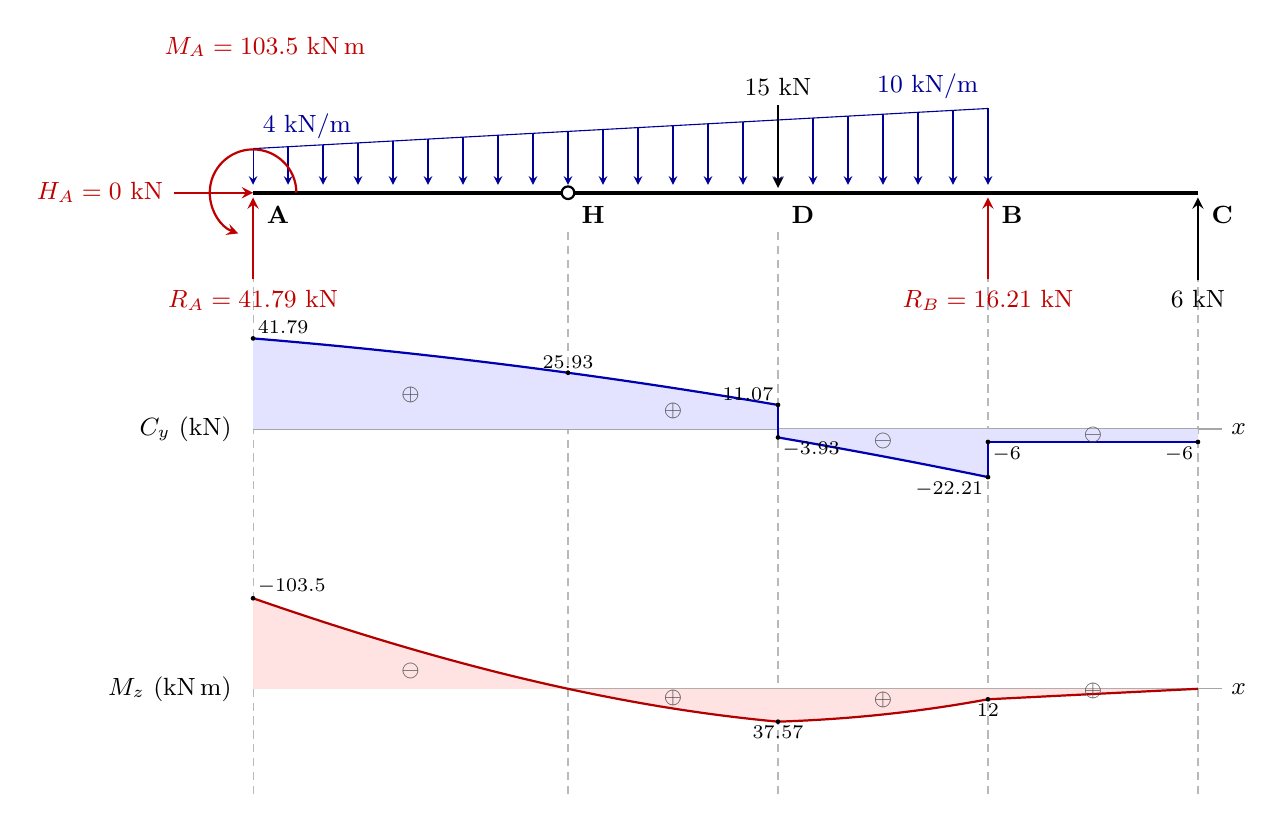
\begin{tikzpicture}
\draw[densely dashed,gray!55] (12.0000,-0.5000) -- (12.0000,-7.7000);
\draw[densely dashed,gray!55] (9.3333,-0.5000) -- (9.3333,-7.7000);
\draw[densely dashed,gray!55] (6.6667,-0.5000) -- (6.6667,-7.7000);
\draw[densely dashed,gray!55] (4.0000,-0.5000) -- (4.0000,-7.7000);
\draw[densely dashed,gray!55] (0.0000,-0.5000) -- (0.0000,-7.7000);
\draw[-stealth,blue!60!black] (0.0000,0.5600) -- (0.0000,0.1000);
\draw[-stealth,blue!60!black] (0.4444,0.5843) -- (0.4444,0.1000);
\draw[-stealth,blue!60!black] (0.8889,0.6086) -- (0.8889,0.1000);
\draw[-stealth,blue!60!black] (1.3333,0.6329) -- (1.3333,0.1000);
\draw[-stealth,blue!60!black] (1.7778,0.6571) -- (1.7778,0.1000);
\draw[-stealth,blue!60!black] (2.2222,0.6814) -- (2.2222,0.1000);
\draw[-stealth,blue!60!black] (2.6667,0.7057) -- (2.6667,0.1000);
\draw[-stealth,blue!60!black] (3.1111,0.7300) -- (3.1111,0.1000);
\draw[-stealth,blue!60!black] (3.5556,0.7543) -- (3.5556,0.1000);
\draw[-stealth,blue!60!black] (4.0000,0.7786) -- (4.0000,0.1000);
\draw[-stealth,blue!60!black] (4.4444,0.8029) -- (4.4444,0.1000);
\draw[-stealth,blue!60!black] (4.8889,0.8271) -- (4.8889,0.1000);
\draw[-stealth,blue!60!black] (5.3333,0.8514) -- (5.3333,0.1000);
\draw[-stealth,blue!60!black] (5.7778,0.8757) -- (5.7778,0.1000);
\draw[-stealth,blue!60!black] (6.2222,0.9000) -- (6.2222,0.1000);
\draw[-stealth,blue!60!black] (6.6667,0.9243) -- (6.6667,0.1000);
\draw[-stealth,blue!60!black] (7.1111,0.9486) -- (7.1111,0.1000);
\draw[-stealth,blue!60!black] (7.5556,0.9729) -- (7.5556,0.1000);
\draw[-stealth,blue!60!black] (8.0000,0.9971) -- (8.0000,0.1000);
\draw[-stealth,blue!60!black] (8.4444,1.0214) -- (8.4444,0.1000);
\draw[-stealth,blue!60!black] (8.8889,1.0457) -- (8.8889,0.1000);
\draw[-stealth,blue!60!black] (9.3333,1.0700) -- (9.3333,0.1000);
% studium:at distributed 0 x=0 to=7 check=span
\draw[blue!60!black] (0.0000,0.5600) -- (0.4444,0.5843) -- (0.8889,0.6086) -- (1.3333,0.6329) -- (1.7778,0.6571) -- (2.2222,0.6814) -- (2.6667,0.7057) -- (3.1111,0.7300) -- (3.5556,0.7543) -- (4.0000,0.7786) -- (4.4444,0.8029) -- (4.8889,0.8271) -- (5.3333,0.8514) -- (5.7778,0.8757) -- (6.2222,0.9000) -- (6.6667,0.9243) -- (7.1111,0.9486) -- (7.5556,0.9729) -- (8.0000,0.9971) -- (8.4444,1.0214) -- (8.8889,1.0457) -- (9.3333,1.0700);
\node[font=\small,anchor=south west,blue!60!black] at (0.0000,0.5600) {$4$~\mbox{kN/m}};
\node[font=\small,anchor=south east,blue!60!black] at (9.3333,1.0700) {$10$~\mbox{kN/m}};
\draw[line width=1.6pt] (0,0.0000) -- (12.0000,0.0000);
% studium:at hinge 0 x=3 check=first
\draw[thick,fill=white] (4.0000,0.0000) circle (0.08);
% studium:at force 0 x=5 check=tip
\draw[-stealth,thick,black] (6.6667,1.1100) -- (6.6667,0.0600);
\node[font=\small,anchor=south] at (6.6667,1.1100) {$15$~\mbox{kN}};
% studium:at force 1 x=9 check=tip
\draw[-stealth,thick,black] (12.0000,-1.1100) -- (12.0000,-0.0600);
\node[font=\small,anchor=north] at (12.0000,-1.1100) {$6$~\mbox{kN}};
% studium:reaction H_A value=0
% studium:at reaction H_A x=0 check=tip
\draw[-stealth,thick,red!75!black] (-1.0000,0.0000) -- (0.0000,0.0000);
\node[font=\small,anchor=east,red!75!black] at (-1.0200,0.0000) {$H_{A} = 0$~\mbox{kN}};
% studium:reaction R_A value=41.79
% studium:at reaction R_A x=0 check=tip
\draw[-stealth,thick,red!75!black] (0.0000,-1.1000) -- (0.0000,-0.0600);
\node[font=\small,anchor=north,red!75!black] at (0.0000,-1.1200) {$R_{A} = 41.79$~\mbox{kN}};
% studium:reaction M_A value=103.5
% studium:at reaction M_A x=0 check=arc
\draw[-stealth,thick,red!75!black] (0.5500,0.0000) arc (0:250:0.55);
\node[font=\small,anchor=south,red!75!black] at (0.1500,1.6000) {$M_{A} = 103.5$~\mbox{kN\,m}};
% studium:reaction R_B value=16.21
% studium:at reaction R_B x=7 check=tip
\draw[-stealth,thick,red!75!black] (9.3333,-1.1000) -- (9.3333,-0.0600);
\node[font=\small,anchor=north,red!75!black] at (9.3333,-1.1200) {$R_{B} = 16.21$~\mbox{kN}};
\node[font=\small\bfseries,anchor=north west] at (0.0500,-0.0500) {A};
\node[font=\small\bfseries,anchor=north west] at (4.0500,-0.0500) {H};
\node[font=\small\bfseries,anchor=north west] at (6.7167,-0.0500) {D};
\node[font=\small\bfseries,anchor=north west] at (9.3833,-0.0500) {B};
\node[font=\small\bfseries,anchor=north west] at (12.0500,-0.0500) {C};
\draw[gray!70] (0,-3.0000) -- (12.3000,-3.0000);
\fill[blue!11] (0.0000,-3.0000) -- (0.0000,-1.8500) -- (0.1250,-1.8604) -- (0.2500,-1.8711) -- (0.3750,-1.8819) -- (0.5000,-1.8929) -- (0.6250,-1.9042) -- (0.7500,-1.9157) -- (0.8750,-1.9273) -- (1.0000,-1.9392) -- (1.1250,-1.9513) -- (1.2500,-1.9636) -- (1.3750,-1.9761) -- (1.5000,-1.9888) -- (1.6250,-2.0017) -- (1.7500,-2.0148) -- (1.8750,-2.0281) -- (2.0000,-2.0417) -- (2.1250,-2.0554) -- (2.2500,-2.0694) -- (2.3750,-2.0835) -- (2.5000,-2.0979) -- (2.6250,-2.1124) -- (2.7500,-2.1272) -- (2.8750,-2.1422) -- (3.0000,-2.1574) -- (3.1250,-2.1728) -- (3.2500,-2.1884) -- (3.3750,-2.2042) -- (3.5000,-2.2202) -- (3.6250,-2.2365) -- (3.7500,-2.2529) -- (3.8750,-2.2696) -- (4.0000,-2.2864) -- (4.0000,-3.0000) -- cycle;
\fill[blue!11] (4.0000,-3.0000) -- (4.0000,-2.2864) -- (4.0833,-2.2978) -- (4.1667,-2.3092) -- (4.2500,-2.3207) -- (4.3333,-2.3324) -- (4.4167,-2.3441) -- (4.5000,-2.3559) -- (4.5833,-2.3678) -- (4.6667,-2.3798) -- (4.7500,-2.3919) -- (4.8333,-2.4041) -- (4.9167,-2.4163) -- (5.0000,-2.4287) -- (5.0833,-2.4411) -- (5.1667,-2.4537) -- (5.2500,-2.4663) -- (5.3333,-2.4791) -- (5.4167,-2.4919) -- (5.5000,-2.5048) -- (5.5833,-2.5178) -- (5.6667,-2.5309) -- (5.7500,-2.5441) -- (5.8333,-2.5574) -- (5.9167,-2.5708) -- (6.0000,-2.5842) -- (6.0833,-2.5978) -- (6.1667,-2.6114) -- (6.2500,-2.6252) -- (6.3333,-2.6390) -- (6.4167,-2.6530) -- (6.5000,-2.6670) -- (6.5833,-2.6811) -- (6.6667,-2.6953) -- (6.6667,-3.0000) -- cycle;
\fill[blue!11] (6.6667,-3.0000) -- (6.6667,-3.1081) -- (6.7500,-3.1224) -- (6.8333,-3.1368) -- (6.9167,-3.1513) -- (7.0000,-3.1659) -- (7.0833,-3.1805) -- (7.1667,-3.1953) -- (7.2500,-3.2101) -- (7.3333,-3.2251) -- (7.4167,-3.2401) -- (7.5000,-3.2552) -- (7.5833,-3.2705) -- (7.6667,-3.2858) -- (7.7500,-3.3012) -- (7.8333,-3.3167) -- (7.9167,-3.3323) -- (8.0000,-3.3479) -- (8.0833,-3.3637) -- (8.1667,-3.3796) -- (8.2500,-3.3955) -- (8.3333,-3.4116) -- (8.4167,-3.4277) -- (8.5000,-3.4440) -- (8.5833,-3.4603) -- (8.6667,-3.4767) -- (8.7500,-3.4932) -- (8.8333,-3.5098) -- (8.9167,-3.5265) -- (9.0000,-3.5433) -- (9.0833,-3.5602) -- (9.1667,-3.5772) -- (9.2500,-3.5942) -- (9.3333,-3.6114) -- (9.3333,-3.0000) -- cycle;
\fill[blue!11] (9.3333,-3.0000) -- (9.3333,-3.1651) -- (12.0000,-3.1651) -- (12.0000,-3.0000) -- cycle;
% studium:series V sx=1.3333333333333333 sy=0.02752136752136752 x0=0.0 y0=-3.0 sign=1
\draw[thick,blue!70!black] (0.0000,-1.8500) -- (0.1250,-1.8604) -- (0.2500,-1.8711) -- (0.3750,-1.8819) -- (0.5000,-1.8929) -- (0.6250,-1.9042) -- (0.7500,-1.9157) -- (0.8750,-1.9273) -- (1.0000,-1.9392) -- (1.1250,-1.9513) -- (1.2500,-1.9636) -- (1.3750,-1.9761) -- (1.5000,-1.9888) -- (1.6250,-2.0017) -- (1.7500,-2.0148) -- (1.8750,-2.0281) -- (2.0000,-2.0417) -- (2.1250,-2.0554) -- (2.2500,-2.0694) -- (2.3750,-2.0835) -- (2.5000,-2.0979) -- (2.6250,-2.1124) -- (2.7500,-2.1272) -- (2.8750,-2.1422) -- (3.0000,-2.1574) -- (3.1250,-2.1728) -- (3.2500,-2.1884) -- (3.3750,-2.2042) -- (3.5000,-2.2202) -- (3.6250,-2.2365) -- (3.7500,-2.2529) -- (3.8750,-2.2696) -- (4.0000,-2.2864);
\draw[thick,blue!70!black] (4.0000,-2.2864) -- (4.0833,-2.2978) -- (4.1667,-2.3092) -- (4.2500,-2.3207) -- (4.3333,-2.3324) -- (4.4167,-2.3441) -- (4.5000,-2.3559) -- (4.5833,-2.3678) -- (4.6667,-2.3798) -- (4.7500,-2.3919) -- (4.8333,-2.4041) -- (4.9167,-2.4163) -- (5.0000,-2.4287) -- (5.0833,-2.4411) -- (5.1667,-2.4537) -- (5.2500,-2.4663) -- (5.3333,-2.4791) -- (5.4167,-2.4919) -- (5.5000,-2.5048) -- (5.5833,-2.5178) -- (5.6667,-2.5309) -- (5.7500,-2.5441) -- (5.8333,-2.5574) -- (5.9167,-2.5708) -- (6.0000,-2.5842) -- (6.0833,-2.5978) -- (6.1667,-2.6114) -- (6.2500,-2.6252) -- (6.3333,-2.6390) -- (6.4167,-2.6530) -- (6.5000,-2.6670) -- (6.5833,-2.6811) -- (6.6667,-2.6953);
\draw[thick,blue!70!black] (6.6667,-3.1081) -- (6.7500,-3.1224) -- (6.8333,-3.1368) -- (6.9167,-3.1513) -- (7.0000,-3.1659) -- (7.0833,-3.1805) -- (7.1667,-3.1953) -- (7.2500,-3.2101) -- (7.3333,-3.2251) -- (7.4167,-3.2401) -- (7.5000,-3.2552) -- (7.5833,-3.2705) -- (7.6667,-3.2858) -- (7.7500,-3.3012) -- (7.8333,-3.3167) -- (7.9167,-3.3323) -- (8.0000,-3.3479) -- (8.0833,-3.3637) -- (8.1667,-3.3796) -- (8.2500,-3.3955) -- (8.3333,-3.4116) -- (8.4167,-3.4277) -- (8.5000,-3.4440) -- (8.5833,-3.4603) -- (8.6667,-3.4767) -- (8.7500,-3.4932) -- (8.8333,-3.5098) -- (8.9167,-3.5265) -- (9.0000,-3.5433) -- (9.0833,-3.5602) -- (9.1667,-3.5772) -- (9.2500,-3.5942) -- (9.3333,-3.6114);
\draw[thick,blue!70!black] (9.3333,-3.1651) -- (12.0000,-3.1651);
% studium:end V
\draw[thick,blue!70!black] (6.6667,-2.6953) -- (6.6667,-3.1081);
\draw[thick,blue!70!black] (9.3333,-3.6114) -- (9.3333,-3.1651);
\node[font=\small,anchor=east] at (-0.15,-3.0000) {$C_y$ (kN)};
\node[font=\small,anchor=west] at (12.3000,-3.0000) {$x$};
% studium:label V x=0 side=right value=41.79
\fill (0.0000,-1.8500) circle (0.03);
\node[font=\scriptsize,anchor=south west,inner sep=1.5pt] at (0.0000,-1.8500) {$41.79$};
% studium:label V x=3 side=both value=25.93
\fill (4.0000,-2.2864) circle (0.03);
\node[font=\scriptsize,anchor=south,inner sep=1.5pt] at (4.0000,-2.2864) {$25.93$};
% studium:label V x=5 side=left value=11.07
\fill (6.6667,-2.6953) circle (0.03);
\node[font=\scriptsize,anchor=south east,inner sep=1.5pt] at (6.6667,-2.6953) {$11.07$};
% studium:label V x=5 side=right value=-3.93
\fill (6.6667,-3.1081) circle (0.03);
\node[font=\scriptsize,anchor=north west,inner sep=1.5pt] at (6.6667,-3.1081) {$-3.93$};
% studium:label V x=7 side=left value=-22.21
\fill (9.3333,-3.6114) circle (0.03);
\node[font=\scriptsize,anchor=north east,inner sep=1.5pt] at (9.3333,-3.6114) {$-22.21$};
% studium:label V x=7 side=right value=-6
\fill (9.3333,-3.1651) circle (0.03);
\node[font=\scriptsize,anchor=north west,inner sep=1.5pt] at (9.3333,-3.1651) {$-6$};
% studium:label V x=9 side=left value=-6
\fill (12.0000,-3.1651) circle (0.03);
\node[font=\scriptsize,anchor=north east,inner sep=1.5pt] at (12.0000,-3.1651) {$-6$};
\node[font=\footnotesize,gray!60!black] at (2.0000,-2.5688) {$\oplus$};
\node[font=\footnotesize,gray!60!black] at (5.3333,-2.7656) {$\oplus$};
\node[font=\footnotesize,gray!60!black] at (8.0000,-3.1566) {$\ominus$};
\node[font=\footnotesize,gray!60!black] at (10.6667,-3.0743) {$\ominus$};
\draw[gray!70] (0,-6.3000) -- (12.3000,-6.3000);
\fill[red!11] (0.0000,-6.3000) -- (0.0000,-5.1500) -- (0.1250,-5.1933) -- (0.2500,-5.2363) -- (0.3750,-5.2788) -- (0.5000,-5.3209) -- (0.6250,-5.3626) -- (0.7500,-5.4038) -- (0.8750,-5.4447) -- (1.0000,-5.4850) -- (1.1250,-5.5250) -- (1.2500,-5.5644) -- (1.3750,-5.6034) -- (1.5000,-5.6419) -- (1.6250,-5.6800) -- (1.7500,-5.7175) -- (1.8750,-5.7545) -- (2.0000,-5.7911) -- (2.1250,-5.8271) -- (2.2500,-5.8626) -- (2.3750,-5.8975) -- (2.5000,-5.9319) -- (2.6250,-5.9658) -- (2.7500,-5.9991) -- (2.8750,-6.0319) -- (3.0000,-6.0641) -- (3.1250,-6.0957) -- (3.2500,-6.1267) -- (3.3750,-6.1571) -- (3.5000,-6.1869) -- (3.6250,-6.2161) -- (3.7500,-6.2447) -- (3.8750,-6.2727) -- (4.0000,-6.3000) -- (4.0000,-6.3000) -- cycle;
\fill[red!11] (4.0000,-6.3000) -- (4.0000,-6.3000) -- (4.0833,-6.3179) -- (4.1667,-6.3354) -- (4.2500,-6.3527) -- (4.3333,-6.3697) -- (4.4167,-6.3864) -- (4.5000,-6.4028) -- (4.5833,-6.4189) -- (4.6667,-6.4347) -- (4.7500,-6.4502) -- (4.8333,-6.4654) -- (4.9167,-6.4803) -- (5.0000,-6.4949) -- (5.0833,-6.5091) -- (5.1667,-6.5231) -- (5.2500,-6.5367) -- (5.3333,-6.5500) -- (5.4167,-6.5630) -- (5.5000,-6.5756) -- (5.5833,-6.5880) -- (5.6667,-6.6000) -- (5.7500,-6.6116) -- (5.8333,-6.6230) -- (5.9167,-6.6340) -- (6.0000,-6.6446) -- (6.0833,-6.6550) -- (6.1667,-6.6649) -- (6.2500,-6.6746) -- (6.3333,-6.6839) -- (6.4167,-6.6928) -- (6.5000,-6.7014) -- (6.5833,-6.7096) -- (6.6667,-6.7175) -- (6.6667,-6.3000) -- cycle;
\fill[red!11] (6.6667,-6.3000) -- (6.6667,-6.7175) -- (6.7500,-6.7146) -- (6.8333,-6.7113) -- (6.9167,-6.7076) -- (7.0000,-6.7036) -- (7.0833,-6.6993) -- (7.1667,-6.6945) -- (7.2500,-6.6894) -- (7.3333,-6.6839) -- (7.4167,-6.6781) -- (7.5000,-6.6718) -- (7.5833,-6.6652) -- (7.6667,-6.6582) -- (7.7500,-6.6508) -- (7.8333,-6.6430) -- (7.9167,-6.6348) -- (8.0000,-6.6262) -- (8.0833,-6.6172) -- (8.1667,-6.6078) -- (8.2500,-6.5981) -- (8.3333,-6.5879) -- (8.4167,-6.5773) -- (8.5000,-6.5663) -- (8.5833,-6.5549) -- (8.6667,-6.5431) -- (8.7500,-6.5308) -- (8.8333,-6.5182) -- (8.9167,-6.5051) -- (9.0000,-6.4916) -- (9.0833,-6.4777) -- (9.1667,-6.4633) -- (9.2500,-6.4485) -- (9.3333,-6.4333) -- (9.3333,-6.3000) -- cycle;
\fill[red!11] (9.3333,-6.3000) -- (9.3333,-6.4333) -- (12.0000,-6.3000) -- (12.0000,-6.3000) -- cycle;
% studium:series M sx=1.3333333333333333 sy=0.01111111111111111 x0=0.0 y0=-6.3 sign=-1
\draw[thick,red!70!black] (0.0000,-5.1500) -- (0.1250,-5.1933) -- (0.2500,-5.2363) -- (0.3750,-5.2788) -- (0.5000,-5.3209) -- (0.6250,-5.3626) -- (0.7500,-5.4038) -- (0.8750,-5.4447) -- (1.0000,-5.4850) -- (1.1250,-5.5250) -- (1.2500,-5.5644) -- (1.3750,-5.6034) -- (1.5000,-5.6419) -- (1.6250,-5.6800) -- (1.7500,-5.7175) -- (1.8750,-5.7545) -- (2.0000,-5.7911) -- (2.1250,-5.8271) -- (2.2500,-5.8626) -- (2.3750,-5.8975) -- (2.5000,-5.9319) -- (2.6250,-5.9658) -- (2.7500,-5.9991) -- (2.8750,-6.0319) -- (3.0000,-6.0641) -- (3.1250,-6.0957) -- (3.2500,-6.1267) -- (3.3750,-6.1571) -- (3.5000,-6.1869) -- (3.6250,-6.2161) -- (3.7500,-6.2447) -- (3.8750,-6.2727) -- (4.0000,-6.3000);
\draw[thick,red!70!black] (4.0000,-6.3000) -- (4.0833,-6.3179) -- (4.1667,-6.3354) -- (4.2500,-6.3527) -- (4.3333,-6.3697) -- (4.4167,-6.3864) -- (4.5000,-6.4028) -- (4.5833,-6.4189) -- (4.6667,-6.4347) -- (4.7500,-6.4502) -- (4.8333,-6.4654) -- (4.9167,-6.4803) -- (5.0000,-6.4949) -- (5.0833,-6.5091) -- (5.1667,-6.5231) -- (5.2500,-6.5367) -- (5.3333,-6.5500) -- (5.4167,-6.5630) -- (5.5000,-6.5756) -- (5.5833,-6.5880) -- (5.6667,-6.6000) -- (5.7500,-6.6116) -- (5.8333,-6.6230) -- (5.9167,-6.6340) -- (6.0000,-6.6446) -- (6.0833,-6.6550) -- (6.1667,-6.6649) -- (6.2500,-6.6746) -- (6.3333,-6.6839) -- (6.4167,-6.6928) -- (6.5000,-6.7014) -- (6.5833,-6.7096) -- (6.6667,-6.7175);
\draw[thick,red!70!black] (6.6667,-6.7175) -- (6.7500,-6.7146) -- (6.8333,-6.7113) -- (6.9167,-6.7076) -- (7.0000,-6.7036) -- (7.0833,-6.6993) -- (7.1667,-6.6945) -- (7.2500,-6.6894) -- (7.3333,-6.6839) -- (7.4167,-6.6781) -- (7.5000,-6.6718) -- (7.5833,-6.6652) -- (7.6667,-6.6582) -- (7.7500,-6.6508) -- (7.8333,-6.6430) -- (7.9167,-6.6348) -- (8.0000,-6.6262) -- (8.0833,-6.6172) -- (8.1667,-6.6078) -- (8.2500,-6.5981) -- (8.3333,-6.5879) -- (8.4167,-6.5773) -- (8.5000,-6.5663) -- (8.5833,-6.5549) -- (8.6667,-6.5431) -- (8.7500,-6.5308) -- (8.8333,-6.5182) -- (8.9167,-6.5051) -- (9.0000,-6.4916) -- (9.0833,-6.4777) -- (9.1667,-6.4633) -- (9.2500,-6.4485) -- (9.3333,-6.4333);
\draw[thick,red!70!black] (9.3333,-6.4333) -- (12.0000,-6.3000);
% studium:end M
\node[font=\small,anchor=east] at (-0.15,-6.3000) {$M_z$ (kN\,m)};
\node[font=\small,anchor=west] at (12.3000,-6.3000) {$x$};
% studium:label M x=0 side=right value=-103.5
\fill (0.0000,-5.1500) circle (0.03);
\node[font=\scriptsize,anchor=south west,inner sep=1.5pt] at (0.0000,-5.1500) {$-103.5$};
% studium:label M x=5 side=both value=37.57
\fill (6.6667,-6.7175) circle (0.03);
\node[font=\scriptsize,anchor=north,inner sep=1.5pt] at (6.6667,-6.7175) {$37.57$};
% studium:label M x=7 side=both value=12
\fill (9.3333,-6.4333) circle (0.03);
\node[font=\scriptsize,anchor=north,inner sep=1.5pt] at (9.3333,-6.4333) {$12$};
\node[font=\footnotesize,gray!60!black] at (2.0000,-6.0710) {$\ominus$};
\node[font=\footnotesize,gray!60!black] at (5.3333,-6.4125) {$\oplus$};
\node[font=\footnotesize,gray!60!black] at (8.0000,-6.4468) {$\oplus$};
\node[font=\footnotesize,gray!60!black] at (10.6667,-6.3300) {$\oplus$};
\end{tikzpicture}%
\fi
\fi
\endgroup
\par\nopagebreak
\studiumcaption{fig:e2-c03-gerber-esfuerzos}{Diagramas de la viga Gerber: flector nulo en la rótula, saltos del cortante en \(D\), \(B\) y \(C\), y extremos del flector en el empotramiento y en \(D\).}
\end{minipage}\par\medskip

\textbf{Resultado e interpretación.}\[\fitmath{\begin{gathered}R_A = 41.79\ \mathrm{kN}\\R_B = 16.21\ \mathrm{kN}\\M_A = 103.5\ \mathrm{kN\,m}\ \text{(horario)}\\M_{z,\max} = 37.57\ \mathrm{kN\,m}\ (x = 5)\\M_{z,\min} = -103.5\ \mathrm{kN\,m}\ (x = 0)\end{gathered}}\]

La rótula fija un cero del flector en $x = 3$ m: a su izquierda el empotramiento trabaja como una ménsula, con flexión negativa grande, y a su derecha el tramo $HB$ se comporta como una viga apoyada en la rótula y en $B$, con flexión positiva. La fuerza hacia arriba en el voladizo reduce la reacción en $B$ y produce un flector positivo sobre el apoyo.

\par\textbf{Comprobación.} Recalcula los pasos con unidades coherentes y aplica el control específico indicado en la orientación del capítulo.

\textbf{Límites.}\begin{itemize}\item modelo plano de Euler-Bernoulli; no se comprueban flechas\end{itemize}

\textbf{Errores frecuentes.}\begin{itemize}\item tratar la rótula como un apoyo y añadirle una reacción
\item escribir la condición de la rótula con momentos de toda la viga en lugar de los de una de sus partes
\item aplicar la resultante de la carga trapezoidal en el centro del tramo\end{itemize}

\end{studiumworked}

\Needspace{.3\textheight}

\begin{studiumworked}{PRB-0186}

\section{PRB-0186 · Diagramas de esfuerzos y flector máximo}

\textbf{Enunciado.} Una viga $AB$ de 4 m con apoyo fijo en $A$ y apoyo móvil en $B$ soporta su peso como carga uniforme de 3 kN/m y una fuerza de 20 kN aplicada en $C$, a $1.5$ m de $A$, inclinada $60^{\circ}$ por debajo de la horizontal y dirigida hacia $B$. Dibuje los diagramas de axiles, cortantes y flectores y calcule el flector máximo.

\par\medskip\noindent\begin{tabular}{@{}p{.18\linewidth}p{.26\linewidth}p{.48\linewidth}@{}}
\toprule Símbolo & Valor y unidad & Significado\\\midrule
$F$ & $20\,\mathrm{kN}$ & fuerza inclinada\\
$q$ & $3\,\mathrm{kN/m}$ & peso propio\\
\bottomrule\end{tabular}\par\medskip

\par\medskip\noindent\begin{minipage}{\linewidth}
\centering
\begingroup
\setbox0=\hbox{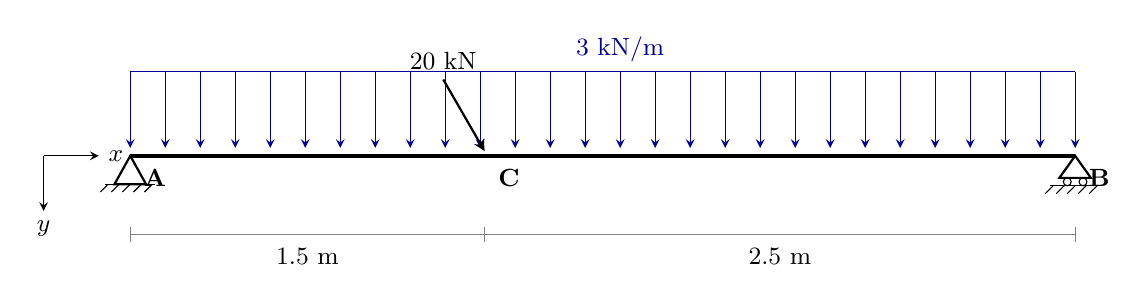
\begin{tikzpicture}
\draw[-stealth,blue!60!black] (0.0000,1.0700) -- (0.0000,0.1000);
\draw[-stealth,blue!60!black] (0.4444,1.0700) -- (0.4444,0.1000);
\draw[-stealth,blue!60!black] (0.8889,1.0700) -- (0.8889,0.1000);
\draw[-stealth,blue!60!black] (1.3333,1.0700) -- (1.3333,0.1000);
\draw[-stealth,blue!60!black] (1.7778,1.0700) -- (1.7778,0.1000);
\draw[-stealth,blue!60!black] (2.2222,1.0700) -- (2.2222,0.1000);
\draw[-stealth,blue!60!black] (2.6667,1.0700) -- (2.6667,0.1000);
\draw[-stealth,blue!60!black] (3.1111,1.0700) -- (3.1111,0.1000);
\draw[-stealth,blue!60!black] (3.5556,1.0700) -- (3.5556,0.1000);
\draw[-stealth,blue!60!black] (4.0000,1.0700) -- (4.0000,0.1000);
\draw[-stealth,blue!60!black] (4.4444,1.0700) -- (4.4444,0.1000);
\draw[-stealth,blue!60!black] (4.8889,1.0700) -- (4.8889,0.1000);
\draw[-stealth,blue!60!black] (5.3333,1.0700) -- (5.3333,0.1000);
\draw[-stealth,blue!60!black] (5.7778,1.0700) -- (5.7778,0.1000);
\draw[-stealth,blue!60!black] (6.2222,1.0700) -- (6.2222,0.1000);
\draw[-stealth,blue!60!black] (6.6667,1.0700) -- (6.6667,0.1000);
\draw[-stealth,blue!60!black] (7.1111,1.0700) -- (7.1111,0.1000);
\draw[-stealth,blue!60!black] (7.5556,1.0700) -- (7.5556,0.1000);
\draw[-stealth,blue!60!black] (8.0000,1.0700) -- (8.0000,0.1000);
\draw[-stealth,blue!60!black] (8.4444,1.0700) -- (8.4444,0.1000);
\draw[-stealth,blue!60!black] (8.8889,1.0700) -- (8.8889,0.1000);
\draw[-stealth,blue!60!black] (9.3333,1.0700) -- (9.3333,0.1000);
\draw[-stealth,blue!60!black] (9.7778,1.0700) -- (9.7778,0.1000);
\draw[-stealth,blue!60!black] (10.2222,1.0700) -- (10.2222,0.1000);
\draw[-stealth,blue!60!black] (10.6667,1.0700) -- (10.6667,0.1000);
\draw[-stealth,blue!60!black] (11.1111,1.0700) -- (11.1111,0.1000);
\draw[-stealth,blue!60!black] (11.5556,1.0700) -- (11.5556,0.1000);
\draw[-stealth,blue!60!black] (12.0000,1.0700) -- (12.0000,0.1000);
% studium:at distributed 0 x=0 to=4 check=span
\draw[blue!60!black] (0.0000,1.0700) -- (0.4444,1.0700) -- (0.8889,1.0700) -- (1.3333,1.0700) -- (1.7778,1.0700) -- (2.2222,1.0700) -- (2.6667,1.0700) -- (3.1111,1.0700) -- (3.5556,1.0700) -- (4.0000,1.0700) -- (4.4444,1.0700) -- (4.8889,1.0700) -- (5.3333,1.0700) -- (5.7778,1.0700) -- (6.2222,1.0700) -- (6.6667,1.0700) -- (7.1111,1.0700) -- (7.5556,1.0700) -- (8.0000,1.0700) -- (8.4444,1.0700) -- (8.8889,1.0700) -- (9.3333,1.0700) -- (9.7778,1.0700) -- (10.2222,1.0700) -- (10.6667,1.0700) -- (11.1111,1.0700) -- (11.5556,1.0700) -- (12.0000,1.0700);
\node[font=\small,anchor=south,blue!60!black] at (6.2222,1.0700) {$3$~\mbox{kN/m}};
\draw[line width=1.6pt] (0,0.0000) -- (12.0000,0.0000);
% studium:at support A x=0 check=first
\draw[thick,fill=white] (0.0000,0.0000) -- (-0.2000,-0.3600) -- (0.2000,-0.3600) -- cycle;
\draw (-0.3200,-0.3600) -- (0.3200,-0.3600);
\draw (-0.2800,-0.3600) -- (-0.3800,-0.4600);
\draw (-0.1400,-0.3600) -- (-0.2400,-0.4600);
\draw (0.0000,-0.3600) -- (-0.1000,-0.4600);
\draw (0.1400,-0.3600) -- (0.0400,-0.4600);
\draw (0.2800,-0.3600) -- (0.1800,-0.4600);
% studium:at support B x=4 check=first
\draw[thick,fill=white] (12.0000,0.0000) -- (11.8000,-0.2800) -- (12.2000,-0.2800) -- cycle;
\draw (11.9000,-0.3300) circle (0.05);
\draw (12.1000,-0.3300) circle (0.05);
\draw (11.6800,-0.3800) -- (12.3200,-0.3800);
\draw (11.7200,-0.3800) -- (11.6200,-0.4800);
\draw (11.8600,-0.3800) -- (11.7600,-0.4800);
\draw (12.0000,-0.3800) -- (11.9000,-0.4800);
\draw (12.1400,-0.3800) -- (12.0400,-0.4800);
\draw (12.2800,-0.3800) -- (12.1800,-0.4800);
% studium:at force 0 x=3/2 check=tip
\draw[-stealth,thick,black] (3.9750,0.9693) -- (4.5000,0.0600);
\node[font=\small,anchor=south] at (3.9750,0.9693) {$20$~\mbox{kN}};
\node[font=\small\bfseries,anchor=north west] at (0.0500,-0.0500) {A};
\node[font=\small\bfseries,anchor=north west] at (4.5500,-0.0500) {C};
\node[font=\small\bfseries,anchor=north west] at (12.0500,-0.0500) {B};
\draw[gray] (0,-1.0000) -- (12.0000,-1.0000);
\draw[gray] (0.0000,-1.1000) -- (0.0000,-0.9000);
\draw[gray] (4.5000,-1.1000) -- (4.5000,-0.9000);
\draw[gray] (12.0000,-1.1000) -- (12.0000,-0.9000);
\node[font=\small,anchor=north] at (2.2500,-1.0500) {$1.5$~\mbox{m}};
\node[font=\small,anchor=north] at (8.2500,-1.0500) {$2.5$~\mbox{m}};
\draw[-stealth] (-1.1,0.0000) -- (-0.4,0.0000) node[right,font=\small] {$x$};
\draw[-stealth] (-1.1,0.0000) -- (-1.1,-0.7000) node[below,font=\small] {$y$};
\end{tikzpicture}}%
\count0=\ht0
\advance\count0 by \dp0
\count2=\wd0
\count4=\dimexpr\textheight/100*38\relax
\count6=\linewidth
\ifnum\count0<1
\count0=1
\fi
\ifnum\count2<1
\count2=1
\fi
\divide\count0 by 4096
\divide\count2 by 4096
\divide\count4 by 4096
\divide\count6 by 4096
\ifnum\count0<1
\count0=1
\fi
\ifnum\count2<1
\count2=1
\fi
\ifnum\count4<1
\count4=1
\fi
\ifnum\count6<1
\count6=1
\fi
\count8=\count2
\ifnum\count0>\count4
\count8=\numexpr\count2*\count4/\count0\relax
\fi
\ifnum\count8>\count6
\resizebox{\linewidth}{!}{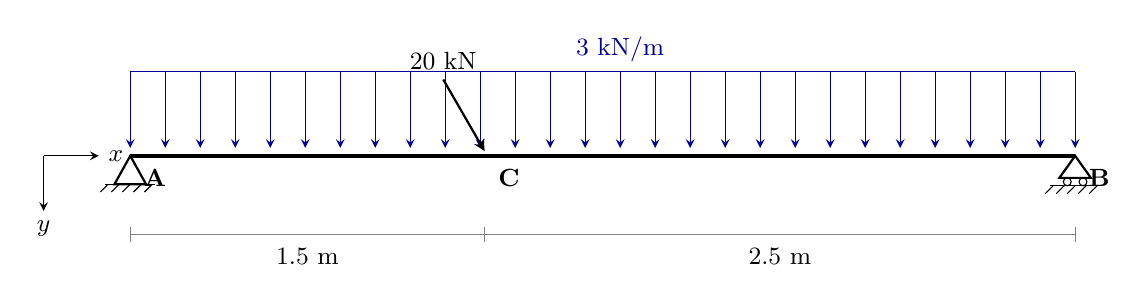
\begin{tikzpicture}
\draw[-stealth,blue!60!black] (0.0000,1.0700) -- (0.0000,0.1000);
\draw[-stealth,blue!60!black] (0.4444,1.0700) -- (0.4444,0.1000);
\draw[-stealth,blue!60!black] (0.8889,1.0700) -- (0.8889,0.1000);
\draw[-stealth,blue!60!black] (1.3333,1.0700) -- (1.3333,0.1000);
\draw[-stealth,blue!60!black] (1.7778,1.0700) -- (1.7778,0.1000);
\draw[-stealth,blue!60!black] (2.2222,1.0700) -- (2.2222,0.1000);
\draw[-stealth,blue!60!black] (2.6667,1.0700) -- (2.6667,0.1000);
\draw[-stealth,blue!60!black] (3.1111,1.0700) -- (3.1111,0.1000);
\draw[-stealth,blue!60!black] (3.5556,1.0700) -- (3.5556,0.1000);
\draw[-stealth,blue!60!black] (4.0000,1.0700) -- (4.0000,0.1000);
\draw[-stealth,blue!60!black] (4.4444,1.0700) -- (4.4444,0.1000);
\draw[-stealth,blue!60!black] (4.8889,1.0700) -- (4.8889,0.1000);
\draw[-stealth,blue!60!black] (5.3333,1.0700) -- (5.3333,0.1000);
\draw[-stealth,blue!60!black] (5.7778,1.0700) -- (5.7778,0.1000);
\draw[-stealth,blue!60!black] (6.2222,1.0700) -- (6.2222,0.1000);
\draw[-stealth,blue!60!black] (6.6667,1.0700) -- (6.6667,0.1000);
\draw[-stealth,blue!60!black] (7.1111,1.0700) -- (7.1111,0.1000);
\draw[-stealth,blue!60!black] (7.5556,1.0700) -- (7.5556,0.1000);
\draw[-stealth,blue!60!black] (8.0000,1.0700) -- (8.0000,0.1000);
\draw[-stealth,blue!60!black] (8.4444,1.0700) -- (8.4444,0.1000);
\draw[-stealth,blue!60!black] (8.8889,1.0700) -- (8.8889,0.1000);
\draw[-stealth,blue!60!black] (9.3333,1.0700) -- (9.3333,0.1000);
\draw[-stealth,blue!60!black] (9.7778,1.0700) -- (9.7778,0.1000);
\draw[-stealth,blue!60!black] (10.2222,1.0700) -- (10.2222,0.1000);
\draw[-stealth,blue!60!black] (10.6667,1.0700) -- (10.6667,0.1000);
\draw[-stealth,blue!60!black] (11.1111,1.0700) -- (11.1111,0.1000);
\draw[-stealth,blue!60!black] (11.5556,1.0700) -- (11.5556,0.1000);
\draw[-stealth,blue!60!black] (12.0000,1.0700) -- (12.0000,0.1000);
% studium:at distributed 0 x=0 to=4 check=span
\draw[blue!60!black] (0.0000,1.0700) -- (0.4444,1.0700) -- (0.8889,1.0700) -- (1.3333,1.0700) -- (1.7778,1.0700) -- (2.2222,1.0700) -- (2.6667,1.0700) -- (3.1111,1.0700) -- (3.5556,1.0700) -- (4.0000,1.0700) -- (4.4444,1.0700) -- (4.8889,1.0700) -- (5.3333,1.0700) -- (5.7778,1.0700) -- (6.2222,1.0700) -- (6.6667,1.0700) -- (7.1111,1.0700) -- (7.5556,1.0700) -- (8.0000,1.0700) -- (8.4444,1.0700) -- (8.8889,1.0700) -- (9.3333,1.0700) -- (9.7778,1.0700) -- (10.2222,1.0700) -- (10.6667,1.0700) -- (11.1111,1.0700) -- (11.5556,1.0700) -- (12.0000,1.0700);
\node[font=\small,anchor=south,blue!60!black] at (6.2222,1.0700) {$3$~\mbox{kN/m}};
\draw[line width=1.6pt] (0,0.0000) -- (12.0000,0.0000);
% studium:at support A x=0 check=first
\draw[thick,fill=white] (0.0000,0.0000) -- (-0.2000,-0.3600) -- (0.2000,-0.3600) -- cycle;
\draw (-0.3200,-0.3600) -- (0.3200,-0.3600);
\draw (-0.2800,-0.3600) -- (-0.3800,-0.4600);
\draw (-0.1400,-0.3600) -- (-0.2400,-0.4600);
\draw (0.0000,-0.3600) -- (-0.1000,-0.4600);
\draw (0.1400,-0.3600) -- (0.0400,-0.4600);
\draw (0.2800,-0.3600) -- (0.1800,-0.4600);
% studium:at support B x=4 check=first
\draw[thick,fill=white] (12.0000,0.0000) -- (11.8000,-0.2800) -- (12.2000,-0.2800) -- cycle;
\draw (11.9000,-0.3300) circle (0.05);
\draw (12.1000,-0.3300) circle (0.05);
\draw (11.6800,-0.3800) -- (12.3200,-0.3800);
\draw (11.7200,-0.3800) -- (11.6200,-0.4800);
\draw (11.8600,-0.3800) -- (11.7600,-0.4800);
\draw (12.0000,-0.3800) -- (11.9000,-0.4800);
\draw (12.1400,-0.3800) -- (12.0400,-0.4800);
\draw (12.2800,-0.3800) -- (12.1800,-0.4800);
% studium:at force 0 x=3/2 check=tip
\draw[-stealth,thick,black] (3.9750,0.9693) -- (4.5000,0.0600);
\node[font=\small,anchor=south] at (3.9750,0.9693) {$20$~\mbox{kN}};
\node[font=\small\bfseries,anchor=north west] at (0.0500,-0.0500) {A};
\node[font=\small\bfseries,anchor=north west] at (4.5500,-0.0500) {C};
\node[font=\small\bfseries,anchor=north west] at (12.0500,-0.0500) {B};
\draw[gray] (0,-1.0000) -- (12.0000,-1.0000);
\draw[gray] (0.0000,-1.1000) -- (0.0000,-0.9000);
\draw[gray] (4.5000,-1.1000) -- (4.5000,-0.9000);
\draw[gray] (12.0000,-1.1000) -- (12.0000,-0.9000);
\node[font=\small,anchor=north] at (2.2500,-1.0500) {$1.5$~\mbox{m}};
\node[font=\small,anchor=north] at (8.2500,-1.0500) {$2.5$~\mbox{m}};
\draw[-stealth] (-1.1,0.0000) -- (-0.4,0.0000) node[right,font=\small] {$x$};
\draw[-stealth] (-1.1,0.0000) -- (-1.1,-0.7000) node[below,font=\small] {$y$};
\end{tikzpicture}}%
\else
\ifnum\count0>\count4
\resizebox{!}{\dimexpr\textheight/100*38\relax}{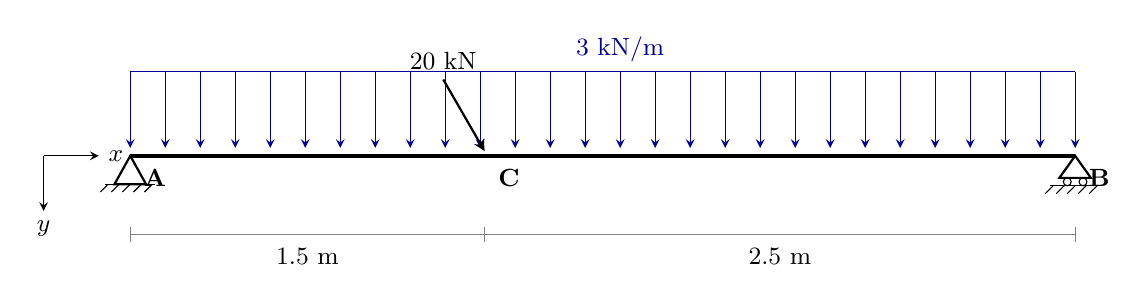
\begin{tikzpicture}
\draw[-stealth,blue!60!black] (0.0000,1.0700) -- (0.0000,0.1000);
\draw[-stealth,blue!60!black] (0.4444,1.0700) -- (0.4444,0.1000);
\draw[-stealth,blue!60!black] (0.8889,1.0700) -- (0.8889,0.1000);
\draw[-stealth,blue!60!black] (1.3333,1.0700) -- (1.3333,0.1000);
\draw[-stealth,blue!60!black] (1.7778,1.0700) -- (1.7778,0.1000);
\draw[-stealth,blue!60!black] (2.2222,1.0700) -- (2.2222,0.1000);
\draw[-stealth,blue!60!black] (2.6667,1.0700) -- (2.6667,0.1000);
\draw[-stealth,blue!60!black] (3.1111,1.0700) -- (3.1111,0.1000);
\draw[-stealth,blue!60!black] (3.5556,1.0700) -- (3.5556,0.1000);
\draw[-stealth,blue!60!black] (4.0000,1.0700) -- (4.0000,0.1000);
\draw[-stealth,blue!60!black] (4.4444,1.0700) -- (4.4444,0.1000);
\draw[-stealth,blue!60!black] (4.8889,1.0700) -- (4.8889,0.1000);
\draw[-stealth,blue!60!black] (5.3333,1.0700) -- (5.3333,0.1000);
\draw[-stealth,blue!60!black] (5.7778,1.0700) -- (5.7778,0.1000);
\draw[-stealth,blue!60!black] (6.2222,1.0700) -- (6.2222,0.1000);
\draw[-stealth,blue!60!black] (6.6667,1.0700) -- (6.6667,0.1000);
\draw[-stealth,blue!60!black] (7.1111,1.0700) -- (7.1111,0.1000);
\draw[-stealth,blue!60!black] (7.5556,1.0700) -- (7.5556,0.1000);
\draw[-stealth,blue!60!black] (8.0000,1.0700) -- (8.0000,0.1000);
\draw[-stealth,blue!60!black] (8.4444,1.0700) -- (8.4444,0.1000);
\draw[-stealth,blue!60!black] (8.8889,1.0700) -- (8.8889,0.1000);
\draw[-stealth,blue!60!black] (9.3333,1.0700) -- (9.3333,0.1000);
\draw[-stealth,blue!60!black] (9.7778,1.0700) -- (9.7778,0.1000);
\draw[-stealth,blue!60!black] (10.2222,1.0700) -- (10.2222,0.1000);
\draw[-stealth,blue!60!black] (10.6667,1.0700) -- (10.6667,0.1000);
\draw[-stealth,blue!60!black] (11.1111,1.0700) -- (11.1111,0.1000);
\draw[-stealth,blue!60!black] (11.5556,1.0700) -- (11.5556,0.1000);
\draw[-stealth,blue!60!black] (12.0000,1.0700) -- (12.0000,0.1000);
% studium:at distributed 0 x=0 to=4 check=span
\draw[blue!60!black] (0.0000,1.0700) -- (0.4444,1.0700) -- (0.8889,1.0700) -- (1.3333,1.0700) -- (1.7778,1.0700) -- (2.2222,1.0700) -- (2.6667,1.0700) -- (3.1111,1.0700) -- (3.5556,1.0700) -- (4.0000,1.0700) -- (4.4444,1.0700) -- (4.8889,1.0700) -- (5.3333,1.0700) -- (5.7778,1.0700) -- (6.2222,1.0700) -- (6.6667,1.0700) -- (7.1111,1.0700) -- (7.5556,1.0700) -- (8.0000,1.0700) -- (8.4444,1.0700) -- (8.8889,1.0700) -- (9.3333,1.0700) -- (9.7778,1.0700) -- (10.2222,1.0700) -- (10.6667,1.0700) -- (11.1111,1.0700) -- (11.5556,1.0700) -- (12.0000,1.0700);
\node[font=\small,anchor=south,blue!60!black] at (6.2222,1.0700) {$3$~\mbox{kN/m}};
\draw[line width=1.6pt] (0,0.0000) -- (12.0000,0.0000);
% studium:at support A x=0 check=first
\draw[thick,fill=white] (0.0000,0.0000) -- (-0.2000,-0.3600) -- (0.2000,-0.3600) -- cycle;
\draw (-0.3200,-0.3600) -- (0.3200,-0.3600);
\draw (-0.2800,-0.3600) -- (-0.3800,-0.4600);
\draw (-0.1400,-0.3600) -- (-0.2400,-0.4600);
\draw (0.0000,-0.3600) -- (-0.1000,-0.4600);
\draw (0.1400,-0.3600) -- (0.0400,-0.4600);
\draw (0.2800,-0.3600) -- (0.1800,-0.4600);
% studium:at support B x=4 check=first
\draw[thick,fill=white] (12.0000,0.0000) -- (11.8000,-0.2800) -- (12.2000,-0.2800) -- cycle;
\draw (11.9000,-0.3300) circle (0.05);
\draw (12.1000,-0.3300) circle (0.05);
\draw (11.6800,-0.3800) -- (12.3200,-0.3800);
\draw (11.7200,-0.3800) -- (11.6200,-0.4800);
\draw (11.8600,-0.3800) -- (11.7600,-0.4800);
\draw (12.0000,-0.3800) -- (11.9000,-0.4800);
\draw (12.1400,-0.3800) -- (12.0400,-0.4800);
\draw (12.2800,-0.3800) -- (12.1800,-0.4800);
% studium:at force 0 x=3/2 check=tip
\draw[-stealth,thick,black] (3.9750,0.9693) -- (4.5000,0.0600);
\node[font=\small,anchor=south] at (3.9750,0.9693) {$20$~\mbox{kN}};
\node[font=\small\bfseries,anchor=north west] at (0.0500,-0.0500) {A};
\node[font=\small\bfseries,anchor=north west] at (4.5500,-0.0500) {C};
\node[font=\small\bfseries,anchor=north west] at (12.0500,-0.0500) {B};
\draw[gray] (0,-1.0000) -- (12.0000,-1.0000);
\draw[gray] (0.0000,-1.1000) -- (0.0000,-0.9000);
\draw[gray] (4.5000,-1.1000) -- (4.5000,-0.9000);
\draw[gray] (12.0000,-1.1000) -- (12.0000,-0.9000);
\node[font=\small,anchor=north] at (2.2500,-1.0500) {$1.5$~\mbox{m}};
\node[font=\small,anchor=north] at (8.2500,-1.0500) {$2.5$~\mbox{m}};
\draw[-stealth] (-1.1,0.0000) -- (-0.4,0.0000) node[right,font=\small] {$x$};
\draw[-stealth] (-1.1,0.0000) -- (-1.1,-0.7000) node[below,font=\small] {$y$};
\end{tikzpicture}}%
\else
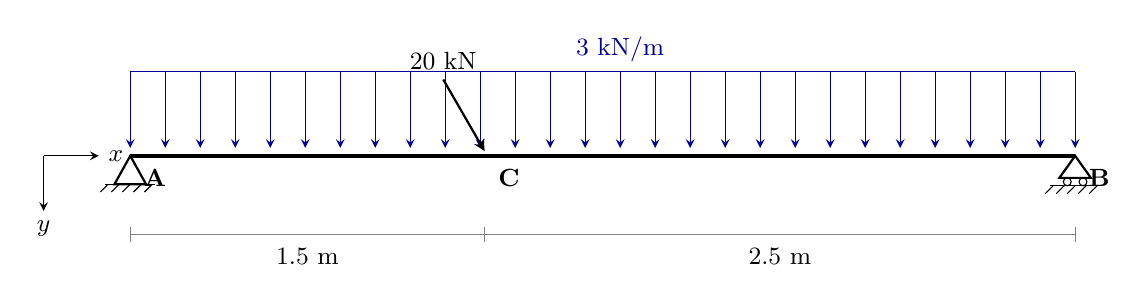
\begin{tikzpicture}
\draw[-stealth,blue!60!black] (0.0000,1.0700) -- (0.0000,0.1000);
\draw[-stealth,blue!60!black] (0.4444,1.0700) -- (0.4444,0.1000);
\draw[-stealth,blue!60!black] (0.8889,1.0700) -- (0.8889,0.1000);
\draw[-stealth,blue!60!black] (1.3333,1.0700) -- (1.3333,0.1000);
\draw[-stealth,blue!60!black] (1.7778,1.0700) -- (1.7778,0.1000);
\draw[-stealth,blue!60!black] (2.2222,1.0700) -- (2.2222,0.1000);
\draw[-stealth,blue!60!black] (2.6667,1.0700) -- (2.6667,0.1000);
\draw[-stealth,blue!60!black] (3.1111,1.0700) -- (3.1111,0.1000);
\draw[-stealth,blue!60!black] (3.5556,1.0700) -- (3.5556,0.1000);
\draw[-stealth,blue!60!black] (4.0000,1.0700) -- (4.0000,0.1000);
\draw[-stealth,blue!60!black] (4.4444,1.0700) -- (4.4444,0.1000);
\draw[-stealth,blue!60!black] (4.8889,1.0700) -- (4.8889,0.1000);
\draw[-stealth,blue!60!black] (5.3333,1.0700) -- (5.3333,0.1000);
\draw[-stealth,blue!60!black] (5.7778,1.0700) -- (5.7778,0.1000);
\draw[-stealth,blue!60!black] (6.2222,1.0700) -- (6.2222,0.1000);
\draw[-stealth,blue!60!black] (6.6667,1.0700) -- (6.6667,0.1000);
\draw[-stealth,blue!60!black] (7.1111,1.0700) -- (7.1111,0.1000);
\draw[-stealth,blue!60!black] (7.5556,1.0700) -- (7.5556,0.1000);
\draw[-stealth,blue!60!black] (8.0000,1.0700) -- (8.0000,0.1000);
\draw[-stealth,blue!60!black] (8.4444,1.0700) -- (8.4444,0.1000);
\draw[-stealth,blue!60!black] (8.8889,1.0700) -- (8.8889,0.1000);
\draw[-stealth,blue!60!black] (9.3333,1.0700) -- (9.3333,0.1000);
\draw[-stealth,blue!60!black] (9.7778,1.0700) -- (9.7778,0.1000);
\draw[-stealth,blue!60!black] (10.2222,1.0700) -- (10.2222,0.1000);
\draw[-stealth,blue!60!black] (10.6667,1.0700) -- (10.6667,0.1000);
\draw[-stealth,blue!60!black] (11.1111,1.0700) -- (11.1111,0.1000);
\draw[-stealth,blue!60!black] (11.5556,1.0700) -- (11.5556,0.1000);
\draw[-stealth,blue!60!black] (12.0000,1.0700) -- (12.0000,0.1000);
% studium:at distributed 0 x=0 to=4 check=span
\draw[blue!60!black] (0.0000,1.0700) -- (0.4444,1.0700) -- (0.8889,1.0700) -- (1.3333,1.0700) -- (1.7778,1.0700) -- (2.2222,1.0700) -- (2.6667,1.0700) -- (3.1111,1.0700) -- (3.5556,1.0700) -- (4.0000,1.0700) -- (4.4444,1.0700) -- (4.8889,1.0700) -- (5.3333,1.0700) -- (5.7778,1.0700) -- (6.2222,1.0700) -- (6.6667,1.0700) -- (7.1111,1.0700) -- (7.5556,1.0700) -- (8.0000,1.0700) -- (8.4444,1.0700) -- (8.8889,1.0700) -- (9.3333,1.0700) -- (9.7778,1.0700) -- (10.2222,1.0700) -- (10.6667,1.0700) -- (11.1111,1.0700) -- (11.5556,1.0700) -- (12.0000,1.0700);
\node[font=\small,anchor=south,blue!60!black] at (6.2222,1.0700) {$3$~\mbox{kN/m}};
\draw[line width=1.6pt] (0,0.0000) -- (12.0000,0.0000);
% studium:at support A x=0 check=first
\draw[thick,fill=white] (0.0000,0.0000) -- (-0.2000,-0.3600) -- (0.2000,-0.3600) -- cycle;
\draw (-0.3200,-0.3600) -- (0.3200,-0.3600);
\draw (-0.2800,-0.3600) -- (-0.3800,-0.4600);
\draw (-0.1400,-0.3600) -- (-0.2400,-0.4600);
\draw (0.0000,-0.3600) -- (-0.1000,-0.4600);
\draw (0.1400,-0.3600) -- (0.0400,-0.4600);
\draw (0.2800,-0.3600) -- (0.1800,-0.4600);
% studium:at support B x=4 check=first
\draw[thick,fill=white] (12.0000,0.0000) -- (11.8000,-0.2800) -- (12.2000,-0.2800) -- cycle;
\draw (11.9000,-0.3300) circle (0.05);
\draw (12.1000,-0.3300) circle (0.05);
\draw (11.6800,-0.3800) -- (12.3200,-0.3800);
\draw (11.7200,-0.3800) -- (11.6200,-0.4800);
\draw (11.8600,-0.3800) -- (11.7600,-0.4800);
\draw (12.0000,-0.3800) -- (11.9000,-0.4800);
\draw (12.1400,-0.3800) -- (12.0400,-0.4800);
\draw (12.2800,-0.3800) -- (12.1800,-0.4800);
% studium:at force 0 x=3/2 check=tip
\draw[-stealth,thick,black] (3.9750,0.9693) -- (4.5000,0.0600);
\node[font=\small,anchor=south] at (3.9750,0.9693) {$20$~\mbox{kN}};
\node[font=\small\bfseries,anchor=north west] at (0.0500,-0.0500) {A};
\node[font=\small\bfseries,anchor=north west] at (4.5500,-0.0500) {C};
\node[font=\small\bfseries,anchor=north west] at (12.0500,-0.0500) {B};
\draw[gray] (0,-1.0000) -- (12.0000,-1.0000);
\draw[gray] (0.0000,-1.1000) -- (0.0000,-0.9000);
\draw[gray] (4.5000,-1.1000) -- (4.5000,-0.9000);
\draw[gray] (12.0000,-1.1000) -- (12.0000,-0.9000);
\node[font=\small,anchor=north] at (2.2500,-1.0500) {$1.5$~\mbox{m}};
\node[font=\small,anchor=north] at (8.2500,-1.0500) {$2.5$~\mbox{m}};
\draw[-stealth] (-1.1,0.0000) -- (-0.4,0.0000) node[right,font=\small] {$x$};
\draw[-stealth] (-1.1,0.0000) -- (-1.1,-0.7000) node[below,font=\small] {$y$};
\end{tikzpicture}%
\fi
\fi
\endgroup
\par\nopagebreak
\studiumcaption{fig:e2-c03-incl-enunciado}{Viga biapoyada con peso propio y fuerza inclinada en \(C\).}
\end{minipage}\par\medskip

\textbf{Hipótesis.}\begin{itemize}\item viga isostática
\item axil positivo de tracción\end{itemize}

\textbf{Modelo y desarrollo.}

Componentes de la fuerza.\[\fitmath{F_x = F\cos 60^{\circ},\qquad F_y = F\sin 60^{\circ}}\]

\textbf{Procedimiento.}\begin{itemize}\item La fuerza tiene una componente horizontal de $10$ kN hacia $B$ y una vertical de $17.32$ kN hacia abajo.
\item Solo el apoyo fijo resiste fuerzas horizontales, así que su reacción horizontal equilibra la componente de $10$ kN; el tramo $AC$ queda traccionado y el $CB$ sin axil.
\item Las reacciones verticales salen de los momentos respecto a $A$ y del equilibrio vertical con la componente vertical y el peso.
\item El cortante cambia de signo en $C$, donde salta la componente vertical, y allí está el flector máximo.\end{itemize}

\textbf{Cálculo de los pasos.}

\begin{enumerate}

\item Componente vertical de la fuerza.

\[\fitmath{y_{1}=\frac{20\cdot \sqrt{3}}{2}\approx 17.32051\,\mathrm{kN}}\]

\item Reacción vertical en B.

\[\fitmath{y_{2}=\frac{\frac{20\cdot \sqrt{3}}{2}\cdot 1.5+3\cdot 4\cdot 2}{4}\approx 12.49519\,\mathrm{kN}}\]

\item Reacción vertical en A.

\[\fitmath{y_{3}=\frac{20\cdot \sqrt{3}}{2}+3\cdot 4-\frac{\frac{20\cdot \sqrt{3}}{2}\cdot 1.5+3\cdot 4\cdot 2}{4}\approx 16.82532\,\mathrm{kN}}\]

\item Flector máximo, en C.

\[\fitmath{y_{4}=\left(\frac{20\cdot \sqrt{3}}{2}+3\cdot 4-\frac{\frac{20\cdot \sqrt{3}}{2}\cdot 1.5+3\cdot 4\cdot 2}{4}\right)\cdot 1.5-\frac{3\cdot {1.5}^{2}}{2}\approx 21.86298\,\mathrm{kN m}}\]

\end{enumerate}

\par\medskip\noindent\begin{minipage}{\linewidth}
\centering
\begingroup
\setbox0=\hbox{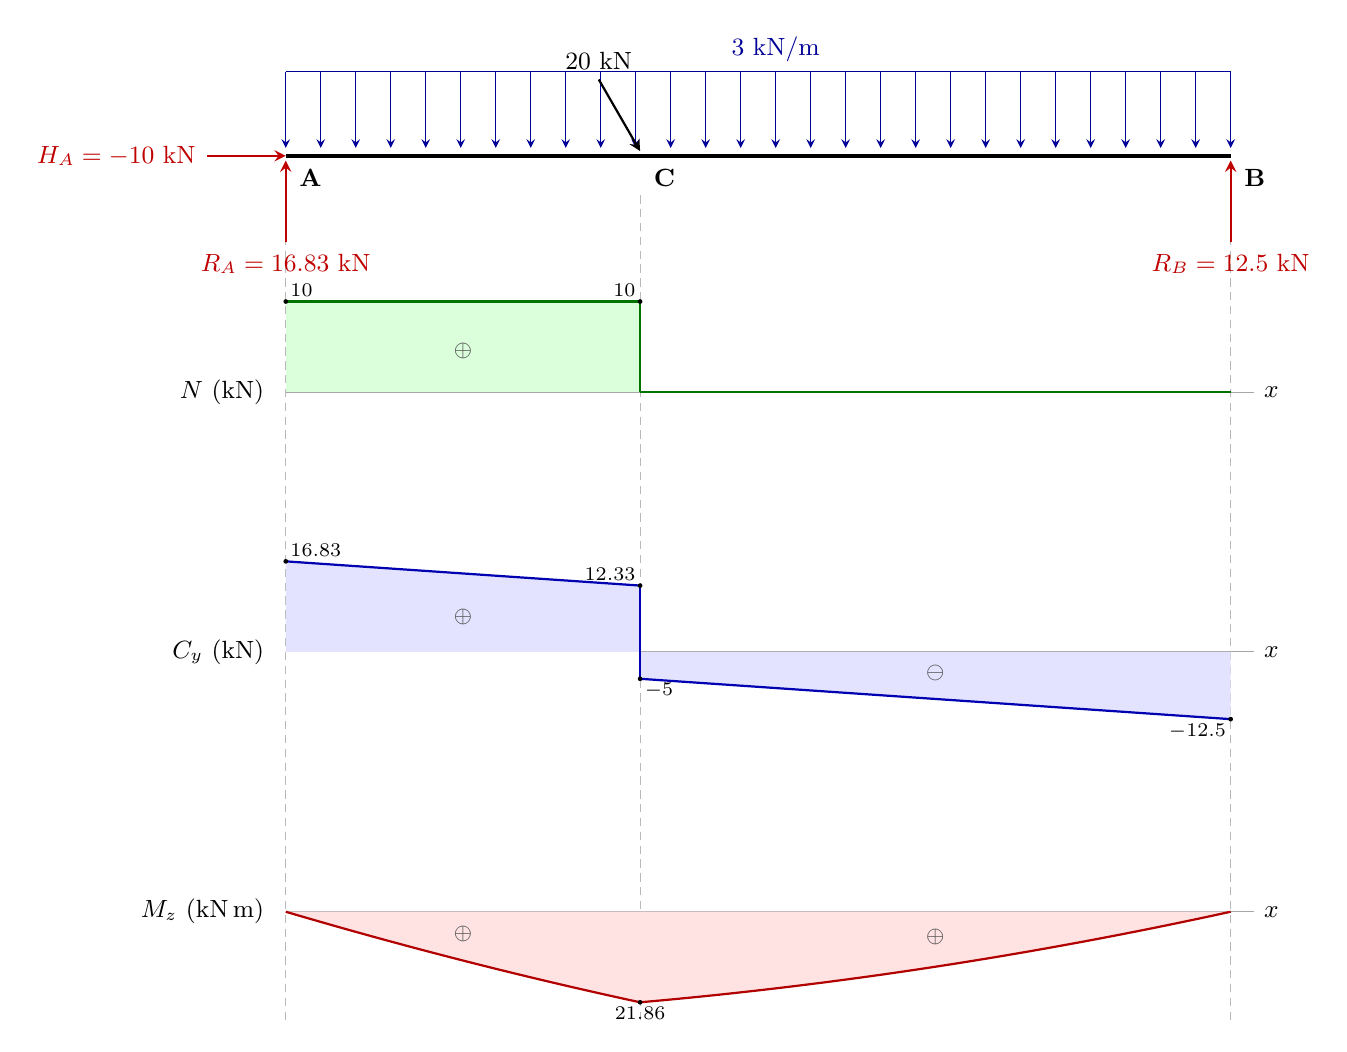
\begin{tikzpicture}
\draw[densely dashed,gray!55] (12.0000,-0.5000) -- (12.0000,-11.0000);
\draw[densely dashed,gray!55] (4.5000,-0.5000) -- (4.5000,-11.0000);
\draw[densely dashed,gray!55] (0.0000,-0.5000) -- (0.0000,-11.0000);
\draw[-stealth,blue!60!black] (0.0000,1.0700) -- (0.0000,0.1000);
\draw[-stealth,blue!60!black] (0.4444,1.0700) -- (0.4444,0.1000);
\draw[-stealth,blue!60!black] (0.8889,1.0700) -- (0.8889,0.1000);
\draw[-stealth,blue!60!black] (1.3333,1.0700) -- (1.3333,0.1000);
\draw[-stealth,blue!60!black] (1.7778,1.0700) -- (1.7778,0.1000);
\draw[-stealth,blue!60!black] (2.2222,1.0700) -- (2.2222,0.1000);
\draw[-stealth,blue!60!black] (2.6667,1.0700) -- (2.6667,0.1000);
\draw[-stealth,blue!60!black] (3.1111,1.0700) -- (3.1111,0.1000);
\draw[-stealth,blue!60!black] (3.5556,1.0700) -- (3.5556,0.1000);
\draw[-stealth,blue!60!black] (4.0000,1.0700) -- (4.0000,0.1000);
\draw[-stealth,blue!60!black] (4.4444,1.0700) -- (4.4444,0.1000);
\draw[-stealth,blue!60!black] (4.8889,1.0700) -- (4.8889,0.1000);
\draw[-stealth,blue!60!black] (5.3333,1.0700) -- (5.3333,0.1000);
\draw[-stealth,blue!60!black] (5.7778,1.0700) -- (5.7778,0.1000);
\draw[-stealth,blue!60!black] (6.2222,1.0700) -- (6.2222,0.1000);
\draw[-stealth,blue!60!black] (6.6667,1.0700) -- (6.6667,0.1000);
\draw[-stealth,blue!60!black] (7.1111,1.0700) -- (7.1111,0.1000);
\draw[-stealth,blue!60!black] (7.5556,1.0700) -- (7.5556,0.1000);
\draw[-stealth,blue!60!black] (8.0000,1.0700) -- (8.0000,0.1000);
\draw[-stealth,blue!60!black] (8.4444,1.0700) -- (8.4444,0.1000);
\draw[-stealth,blue!60!black] (8.8889,1.0700) -- (8.8889,0.1000);
\draw[-stealth,blue!60!black] (9.3333,1.0700) -- (9.3333,0.1000);
\draw[-stealth,blue!60!black] (9.7778,1.0700) -- (9.7778,0.1000);
\draw[-stealth,blue!60!black] (10.2222,1.0700) -- (10.2222,0.1000);
\draw[-stealth,blue!60!black] (10.6667,1.0700) -- (10.6667,0.1000);
\draw[-stealth,blue!60!black] (11.1111,1.0700) -- (11.1111,0.1000);
\draw[-stealth,blue!60!black] (11.5556,1.0700) -- (11.5556,0.1000);
\draw[-stealth,blue!60!black] (12.0000,1.0700) -- (12.0000,0.1000);
% studium:at distributed 0 x=0 to=4 check=span
\draw[blue!60!black] (0.0000,1.0700) -- (0.4444,1.0700) -- (0.8889,1.0700) -- (1.3333,1.0700) -- (1.7778,1.0700) -- (2.2222,1.0700) -- (2.6667,1.0700) -- (3.1111,1.0700) -- (3.5556,1.0700) -- (4.0000,1.0700) -- (4.4444,1.0700) -- (4.8889,1.0700) -- (5.3333,1.0700) -- (5.7778,1.0700) -- (6.2222,1.0700) -- (6.6667,1.0700) -- (7.1111,1.0700) -- (7.5556,1.0700) -- (8.0000,1.0700) -- (8.4444,1.0700) -- (8.8889,1.0700) -- (9.3333,1.0700) -- (9.7778,1.0700) -- (10.2222,1.0700) -- (10.6667,1.0700) -- (11.1111,1.0700) -- (11.5556,1.0700) -- (12.0000,1.0700);
\node[font=\small,anchor=south,blue!60!black] at (6.2222,1.0700) {$3$~\mbox{kN/m}};
\draw[line width=1.6pt] (0,0.0000) -- (12.0000,0.0000);
% studium:at force 0 x=3/2 check=tip
\draw[-stealth,thick,black] (3.9750,0.9693) -- (4.5000,0.0600);
\node[font=\small,anchor=south] at (3.9750,0.9693) {$20$~\mbox{kN}};
% studium:reaction H_A value=-10
% studium:at reaction H_A x=0 check=tip
\draw[-stealth,thick,red!75!black] (-1.0000,0.0000) -- (0.0000,0.0000);
\node[font=\small,anchor=east,red!75!black] at (-1.0200,0.0000) {$H_{A} = -10$~\mbox{kN}};
% studium:reaction R_A value=16.83
% studium:at reaction R_A x=0 check=tip
\draw[-stealth,thick,red!75!black] (0.0000,-1.1000) -- (0.0000,-0.0600);
\node[font=\small,anchor=north,red!75!black] at (0.0000,-1.1200) {$R_{A} = 16.83$~\mbox{kN}};
% studium:reaction R_B value=12.5
% studium:at reaction R_B x=4 check=tip
\draw[-stealth,thick,red!75!black] (12.0000,-1.1000) -- (12.0000,-0.0600);
\node[font=\small,anchor=north,red!75!black] at (12.0000,-1.1200) {$R_{B} = 12.5$~\mbox{kN}};
\node[font=\small\bfseries,anchor=north west] at (0.0500,-0.0500) {A};
\node[font=\small\bfseries,anchor=north west] at (4.5500,-0.0500) {C};
\node[font=\small\bfseries,anchor=north west] at (12.0500,-0.0500) {B};
\draw[gray!70] (0,-3.0000) -- (12.3000,-3.0000);
\fill[green!14] (0.0000,-3.0000) -- (0.0000,-1.8500) -- (4.5000,-1.8500) -- (4.5000,-3.0000) -- cycle;
\fill[green!14] (4.5000,-3.0000) -- (4.5000,-3.0000) -- (12.0000,-3.0000) -- (12.0000,-3.0000) -- cycle;
% studium:series N sx=3.0 sy=0.11499999999999999 x0=0.0 y0=-3.0 sign=1
\draw[thick,green!45!black] (0.0000,-1.8500) -- (4.5000,-1.8500);
\draw[thick,green!45!black] (4.5000,-3.0000) -- (12.0000,-3.0000);
% studium:end N
\draw[thick,green!45!black] (4.5000,-1.8500) -- (4.5000,-3.0000);
\node[font=\small,anchor=east] at (-0.15,-3.0000) {$N$ (kN)};
\node[font=\small,anchor=west] at (12.3000,-3.0000) {$x$};
% studium:label N x=0 side=right value=10
\fill (0.0000,-1.8500) circle (0.03);
\node[font=\scriptsize,anchor=south west,inner sep=1.5pt] at (0.0000,-1.8500) {$10$};
% studium:label N x=3/2 side=left value=10
\fill (4.5000,-1.8500) circle (0.03);
\node[font=\scriptsize,anchor=south east,inner sep=1.5pt] at (4.5000,-1.8500) {$10$};
\node[font=\footnotesize,gray!60!black] at (2.2500,-2.4825) {$\oplus$};
\draw[gray!70] (0,-6.3000) -- (12.3000,-6.3000);
\fill[blue!11] (0.0000,-6.3000) -- (0.0000,-5.1500) -- (4.5000,-5.4576) -- (4.5000,-6.3000) -- cycle;
\fill[blue!11] (4.5000,-6.3000) -- (4.5000,-6.6414) -- (12.0000,-7.1540) -- (12.0000,-6.3000) -- cycle;
% studium:series V sx=3.0 sy=0.06834937865313385 x0=0.0 y0=-6.3 sign=1
\draw[thick,blue!70!black] (0.0000,-5.1500) -- (4.5000,-5.4576);
\draw[thick,blue!70!black] (4.5000,-6.6414) -- (12.0000,-7.1540);
% studium:end V
\draw[thick,blue!70!black] (4.5000,-5.4576) -- (4.5000,-6.6414);
\node[font=\small,anchor=east] at (-0.15,-6.3000) {$C_y$ (kN)};
\node[font=\small,anchor=west] at (12.3000,-6.3000) {$x$};
% studium:label V x=0 side=right value=16.83
\fill (0.0000,-5.1500) circle (0.03);
\node[font=\scriptsize,anchor=south west,inner sep=1.5pt] at (0.0000,-5.1500) {$16.83$};
% studium:label V x=3/2 side=left value=12.33
\fill (4.5000,-5.4576) circle (0.03);
\node[font=\scriptsize,anchor=south east,inner sep=1.5pt] at (4.5000,-5.4576) {$12.33$};
% studium:label V x=3/2 side=right value=-5
\fill (4.5000,-6.6414) circle (0.03);
\node[font=\scriptsize,anchor=north west,inner sep=1.5pt] at (4.5000,-6.6414) {$-5$};
% studium:label V x=4 side=left value=-12.5
\fill (12.0000,-7.1540) circle (0.03);
\node[font=\scriptsize,anchor=north east,inner sep=1.5pt] at (12.0000,-7.1540) {$-12.5$};
\node[font=\footnotesize,gray!60!black] at (2.2500,-5.8517) {$\oplus$};
\node[font=\footnotesize,gray!60!black] at (8.2500,-6.5690) {$\ominus$};
\draw[gray!70] (0,-9.6000) -- (12.3000,-9.6000);
\fill[red!11] (0.0000,-9.6000) -- (0.0000,-9.6000) -- (0.1406,-9.6413) -- (0.2812,-9.6823) -- (0.4219,-9.7229) -- (0.5625,-9.7632) -- (0.7031,-9.8031) -- (0.8438,-9.8427) -- (0.9844,-9.8819) -- (1.1250,-9.9208) -- (1.2656,-9.9593) -- (1.4062,-9.9975) -- (1.5469,-10.0354) -- (1.6875,-10.0729) -- (1.8281,-10.1100) -- (1.9688,-10.1468) -- (2.1094,-10.1833) -- (2.2500,-10.2194) -- (2.3906,-10.2551) -- (2.5312,-10.2906) -- (2.6719,-10.3256) -- (2.8125,-10.3604) -- (2.9531,-10.3947) -- (3.0938,-10.4288) -- (3.2344,-10.4624) -- (3.3750,-10.4958) -- (3.5156,-10.5288) -- (3.6562,-10.5614) -- (3.7969,-10.5937) -- (3.9375,-10.6257) -- (4.0781,-10.6573) -- (4.2188,-10.6885) -- (4.3594,-10.7194) -- (4.5000,-10.7500) -- (4.5000,-9.6000) -- cycle;
\fill[red!11] (4.5000,-9.6000) -- (4.5000,-10.7500) -- (4.7344,-10.7290) -- (4.9688,-10.7070) -- (5.2031,-10.6841) -- (5.4375,-10.6602) -- (5.6719,-10.6353) -- (5.9062,-10.6095) -- (6.1406,-10.5827) -- (6.3750,-10.5550) -- (6.6094,-10.5262) -- (6.8438,-10.4966) -- (7.0781,-10.4659) -- (7.3125,-10.4343) -- (7.5469,-10.4018) -- (7.7812,-10.3682) -- (8.0156,-10.3337) -- (8.2500,-10.2983) -- (8.4844,-10.2619) -- (8.7188,-10.2245) -- (8.9531,-10.1861) -- (9.1875,-10.1468) -- (9.4219,-10.1066) -- (9.6562,-10.0653) -- (9.8906,-10.0231) -- (10.1250,-9.9800) -- (10.3594,-9.9358) -- (10.5938,-9.8907) -- (10.8281,-9.8447) -- (11.0625,-9.7977) -- (11.2969,-9.7497) -- (11.5312,-9.7008) -- (11.7656,-9.6509) -- (12.0000,-9.6000) -- (12.0000,-9.6000) -- cycle;
% studium:series M sx=3.0 sy=0.0526003405537054 x0=0.0 y0=-9.6 sign=-1
\draw[thick,red!70!black] (0.0000,-9.6000) -- (0.1406,-9.6413) -- (0.2812,-9.6823) -- (0.4219,-9.7229) -- (0.5625,-9.7632) -- (0.7031,-9.8031) -- (0.8438,-9.8427) -- (0.9844,-9.8819) -- (1.1250,-9.9208) -- (1.2656,-9.9593) -- (1.4062,-9.9975) -- (1.5469,-10.0354) -- (1.6875,-10.0729) -- (1.8281,-10.1100) -- (1.9688,-10.1468) -- (2.1094,-10.1833) -- (2.2500,-10.2194) -- (2.3906,-10.2551) -- (2.5312,-10.2906) -- (2.6719,-10.3256) -- (2.8125,-10.3604) -- (2.9531,-10.3947) -- (3.0938,-10.4288) -- (3.2344,-10.4624) -- (3.3750,-10.4958) -- (3.5156,-10.5288) -- (3.6562,-10.5614) -- (3.7969,-10.5937) -- (3.9375,-10.6257) -- (4.0781,-10.6573) -- (4.2188,-10.6885) -- (4.3594,-10.7194) -- (4.5000,-10.7500);
\draw[thick,red!70!black] (4.5000,-10.7500) -- (4.7344,-10.7290) -- (4.9688,-10.7070) -- (5.2031,-10.6841) -- (5.4375,-10.6602) -- (5.6719,-10.6353) -- (5.9062,-10.6095) -- (6.1406,-10.5827) -- (6.3750,-10.5550) -- (6.6094,-10.5262) -- (6.8438,-10.4966) -- (7.0781,-10.4659) -- (7.3125,-10.4343) -- (7.5469,-10.4018) -- (7.7812,-10.3682) -- (8.0156,-10.3337) -- (8.2500,-10.2983) -- (8.4844,-10.2619) -- (8.7188,-10.2245) -- (8.9531,-10.1861) -- (9.1875,-10.1468) -- (9.4219,-10.1066) -- (9.6562,-10.0653) -- (9.8906,-10.0231) -- (10.1250,-9.9800) -- (10.3594,-9.9358) -- (10.5938,-9.8907) -- (10.8281,-9.8447) -- (11.0625,-9.7977) -- (11.2969,-9.7497) -- (11.5312,-9.7008) -- (11.7656,-9.6509) -- (12.0000,-9.6000);
% studium:end M
\node[font=\small,anchor=east] at (-0.15,-9.6000) {$M_z$ (kN\,m)};
\node[font=\small,anchor=west] at (12.3000,-9.6000) {$x$};
% studium:label M x=3/2 side=both value=21.86
\fill (4.5000,-10.7500) circle (0.03);
\node[font=\scriptsize,anchor=north,inner sep=1.5pt] at (4.5000,-10.7500) {$21.86$};
\node[font=\footnotesize,gray!60!black] at (2.2500,-9.8787) {$\oplus$};
\node[font=\footnotesize,gray!60!black] at (8.2500,-9.9142) {$\oplus$};
\end{tikzpicture}}%
\count0=\ht0
\advance\count0 by \dp0
\count2=\wd0
\count4=\dimexpr\textheight/100*38\relax
\count6=\linewidth
\ifnum\count0<1
\count0=1
\fi
\ifnum\count2<1
\count2=1
\fi
\divide\count0 by 4096
\divide\count2 by 4096
\divide\count4 by 4096
\divide\count6 by 4096
\ifnum\count0<1
\count0=1
\fi
\ifnum\count2<1
\count2=1
\fi
\ifnum\count4<1
\count4=1
\fi
\ifnum\count6<1
\count6=1
\fi
\count8=\count2
\ifnum\count0>\count4
\count8=\numexpr\count2*\count4/\count0\relax
\fi
\ifnum\count8>\count6
\resizebox{\linewidth}{!}{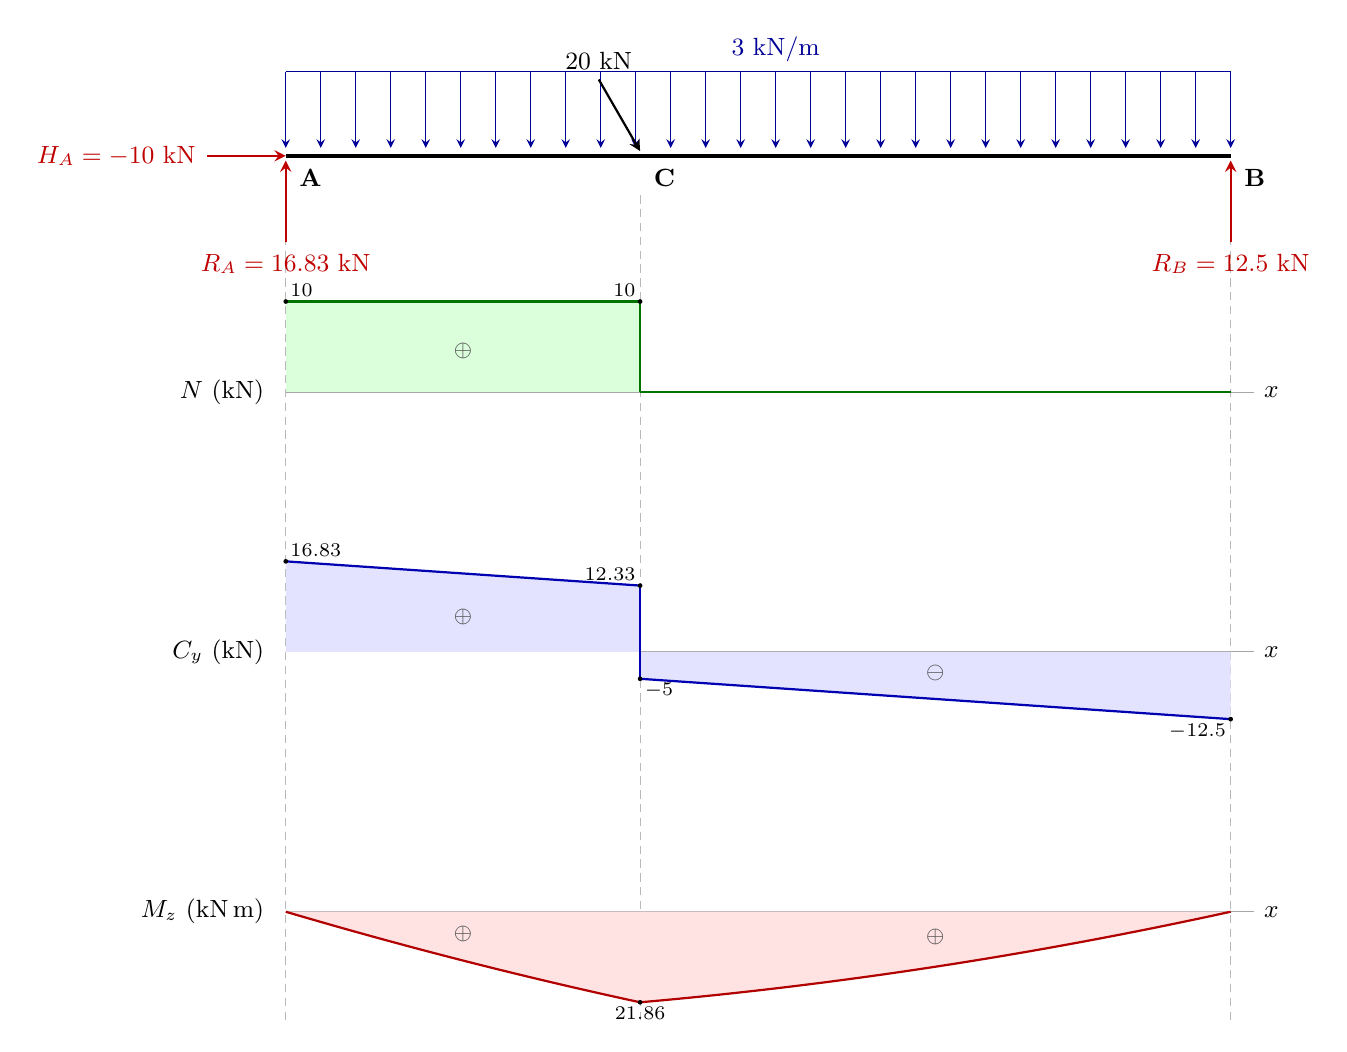
\begin{tikzpicture}
\draw[densely dashed,gray!55] (12.0000,-0.5000) -- (12.0000,-11.0000);
\draw[densely dashed,gray!55] (4.5000,-0.5000) -- (4.5000,-11.0000);
\draw[densely dashed,gray!55] (0.0000,-0.5000) -- (0.0000,-11.0000);
\draw[-stealth,blue!60!black] (0.0000,1.0700) -- (0.0000,0.1000);
\draw[-stealth,blue!60!black] (0.4444,1.0700) -- (0.4444,0.1000);
\draw[-stealth,blue!60!black] (0.8889,1.0700) -- (0.8889,0.1000);
\draw[-stealth,blue!60!black] (1.3333,1.0700) -- (1.3333,0.1000);
\draw[-stealth,blue!60!black] (1.7778,1.0700) -- (1.7778,0.1000);
\draw[-stealth,blue!60!black] (2.2222,1.0700) -- (2.2222,0.1000);
\draw[-stealth,blue!60!black] (2.6667,1.0700) -- (2.6667,0.1000);
\draw[-stealth,blue!60!black] (3.1111,1.0700) -- (3.1111,0.1000);
\draw[-stealth,blue!60!black] (3.5556,1.0700) -- (3.5556,0.1000);
\draw[-stealth,blue!60!black] (4.0000,1.0700) -- (4.0000,0.1000);
\draw[-stealth,blue!60!black] (4.4444,1.0700) -- (4.4444,0.1000);
\draw[-stealth,blue!60!black] (4.8889,1.0700) -- (4.8889,0.1000);
\draw[-stealth,blue!60!black] (5.3333,1.0700) -- (5.3333,0.1000);
\draw[-stealth,blue!60!black] (5.7778,1.0700) -- (5.7778,0.1000);
\draw[-stealth,blue!60!black] (6.2222,1.0700) -- (6.2222,0.1000);
\draw[-stealth,blue!60!black] (6.6667,1.0700) -- (6.6667,0.1000);
\draw[-stealth,blue!60!black] (7.1111,1.0700) -- (7.1111,0.1000);
\draw[-stealth,blue!60!black] (7.5556,1.0700) -- (7.5556,0.1000);
\draw[-stealth,blue!60!black] (8.0000,1.0700) -- (8.0000,0.1000);
\draw[-stealth,blue!60!black] (8.4444,1.0700) -- (8.4444,0.1000);
\draw[-stealth,blue!60!black] (8.8889,1.0700) -- (8.8889,0.1000);
\draw[-stealth,blue!60!black] (9.3333,1.0700) -- (9.3333,0.1000);
\draw[-stealth,blue!60!black] (9.7778,1.0700) -- (9.7778,0.1000);
\draw[-stealth,blue!60!black] (10.2222,1.0700) -- (10.2222,0.1000);
\draw[-stealth,blue!60!black] (10.6667,1.0700) -- (10.6667,0.1000);
\draw[-stealth,blue!60!black] (11.1111,1.0700) -- (11.1111,0.1000);
\draw[-stealth,blue!60!black] (11.5556,1.0700) -- (11.5556,0.1000);
\draw[-stealth,blue!60!black] (12.0000,1.0700) -- (12.0000,0.1000);
% studium:at distributed 0 x=0 to=4 check=span
\draw[blue!60!black] (0.0000,1.0700) -- (0.4444,1.0700) -- (0.8889,1.0700) -- (1.3333,1.0700) -- (1.7778,1.0700) -- (2.2222,1.0700) -- (2.6667,1.0700) -- (3.1111,1.0700) -- (3.5556,1.0700) -- (4.0000,1.0700) -- (4.4444,1.0700) -- (4.8889,1.0700) -- (5.3333,1.0700) -- (5.7778,1.0700) -- (6.2222,1.0700) -- (6.6667,1.0700) -- (7.1111,1.0700) -- (7.5556,1.0700) -- (8.0000,1.0700) -- (8.4444,1.0700) -- (8.8889,1.0700) -- (9.3333,1.0700) -- (9.7778,1.0700) -- (10.2222,1.0700) -- (10.6667,1.0700) -- (11.1111,1.0700) -- (11.5556,1.0700) -- (12.0000,1.0700);
\node[font=\small,anchor=south,blue!60!black] at (6.2222,1.0700) {$3$~\mbox{kN/m}};
\draw[line width=1.6pt] (0,0.0000) -- (12.0000,0.0000);
% studium:at force 0 x=3/2 check=tip
\draw[-stealth,thick,black] (3.9750,0.9693) -- (4.5000,0.0600);
\node[font=\small,anchor=south] at (3.9750,0.9693) {$20$~\mbox{kN}};
% studium:reaction H_A value=-10
% studium:at reaction H_A x=0 check=tip
\draw[-stealth,thick,red!75!black] (-1.0000,0.0000) -- (0.0000,0.0000);
\node[font=\small,anchor=east,red!75!black] at (-1.0200,0.0000) {$H_{A} = -10$~\mbox{kN}};
% studium:reaction R_A value=16.83
% studium:at reaction R_A x=0 check=tip
\draw[-stealth,thick,red!75!black] (0.0000,-1.1000) -- (0.0000,-0.0600);
\node[font=\small,anchor=north,red!75!black] at (0.0000,-1.1200) {$R_{A} = 16.83$~\mbox{kN}};
% studium:reaction R_B value=12.5
% studium:at reaction R_B x=4 check=tip
\draw[-stealth,thick,red!75!black] (12.0000,-1.1000) -- (12.0000,-0.0600);
\node[font=\small,anchor=north,red!75!black] at (12.0000,-1.1200) {$R_{B} = 12.5$~\mbox{kN}};
\node[font=\small\bfseries,anchor=north west] at (0.0500,-0.0500) {A};
\node[font=\small\bfseries,anchor=north west] at (4.5500,-0.0500) {C};
\node[font=\small\bfseries,anchor=north west] at (12.0500,-0.0500) {B};
\draw[gray!70] (0,-3.0000) -- (12.3000,-3.0000);
\fill[green!14] (0.0000,-3.0000) -- (0.0000,-1.8500) -- (4.5000,-1.8500) -- (4.5000,-3.0000) -- cycle;
\fill[green!14] (4.5000,-3.0000) -- (4.5000,-3.0000) -- (12.0000,-3.0000) -- (12.0000,-3.0000) -- cycle;
% studium:series N sx=3.0 sy=0.11499999999999999 x0=0.0 y0=-3.0 sign=1
\draw[thick,green!45!black] (0.0000,-1.8500) -- (4.5000,-1.8500);
\draw[thick,green!45!black] (4.5000,-3.0000) -- (12.0000,-3.0000);
% studium:end N
\draw[thick,green!45!black] (4.5000,-1.8500) -- (4.5000,-3.0000);
\node[font=\small,anchor=east] at (-0.15,-3.0000) {$N$ (kN)};
\node[font=\small,anchor=west] at (12.3000,-3.0000) {$x$};
% studium:label N x=0 side=right value=10
\fill (0.0000,-1.8500) circle (0.03);
\node[font=\scriptsize,anchor=south west,inner sep=1.5pt] at (0.0000,-1.8500) {$10$};
% studium:label N x=3/2 side=left value=10
\fill (4.5000,-1.8500) circle (0.03);
\node[font=\scriptsize,anchor=south east,inner sep=1.5pt] at (4.5000,-1.8500) {$10$};
\node[font=\footnotesize,gray!60!black] at (2.2500,-2.4825) {$\oplus$};
\draw[gray!70] (0,-6.3000) -- (12.3000,-6.3000);
\fill[blue!11] (0.0000,-6.3000) -- (0.0000,-5.1500) -- (4.5000,-5.4576) -- (4.5000,-6.3000) -- cycle;
\fill[blue!11] (4.5000,-6.3000) -- (4.5000,-6.6414) -- (12.0000,-7.1540) -- (12.0000,-6.3000) -- cycle;
% studium:series V sx=3.0 sy=0.06834937865313385 x0=0.0 y0=-6.3 sign=1
\draw[thick,blue!70!black] (0.0000,-5.1500) -- (4.5000,-5.4576);
\draw[thick,blue!70!black] (4.5000,-6.6414) -- (12.0000,-7.1540);
% studium:end V
\draw[thick,blue!70!black] (4.5000,-5.4576) -- (4.5000,-6.6414);
\node[font=\small,anchor=east] at (-0.15,-6.3000) {$C_y$ (kN)};
\node[font=\small,anchor=west] at (12.3000,-6.3000) {$x$};
% studium:label V x=0 side=right value=16.83
\fill (0.0000,-5.1500) circle (0.03);
\node[font=\scriptsize,anchor=south west,inner sep=1.5pt] at (0.0000,-5.1500) {$16.83$};
% studium:label V x=3/2 side=left value=12.33
\fill (4.5000,-5.4576) circle (0.03);
\node[font=\scriptsize,anchor=south east,inner sep=1.5pt] at (4.5000,-5.4576) {$12.33$};
% studium:label V x=3/2 side=right value=-5
\fill (4.5000,-6.6414) circle (0.03);
\node[font=\scriptsize,anchor=north west,inner sep=1.5pt] at (4.5000,-6.6414) {$-5$};
% studium:label V x=4 side=left value=-12.5
\fill (12.0000,-7.1540) circle (0.03);
\node[font=\scriptsize,anchor=north east,inner sep=1.5pt] at (12.0000,-7.1540) {$-12.5$};
\node[font=\footnotesize,gray!60!black] at (2.2500,-5.8517) {$\oplus$};
\node[font=\footnotesize,gray!60!black] at (8.2500,-6.5690) {$\ominus$};
\draw[gray!70] (0,-9.6000) -- (12.3000,-9.6000);
\fill[red!11] (0.0000,-9.6000) -- (0.0000,-9.6000) -- (0.1406,-9.6413) -- (0.2812,-9.6823) -- (0.4219,-9.7229) -- (0.5625,-9.7632) -- (0.7031,-9.8031) -- (0.8438,-9.8427) -- (0.9844,-9.8819) -- (1.1250,-9.9208) -- (1.2656,-9.9593) -- (1.4062,-9.9975) -- (1.5469,-10.0354) -- (1.6875,-10.0729) -- (1.8281,-10.1100) -- (1.9688,-10.1468) -- (2.1094,-10.1833) -- (2.2500,-10.2194) -- (2.3906,-10.2551) -- (2.5312,-10.2906) -- (2.6719,-10.3256) -- (2.8125,-10.3604) -- (2.9531,-10.3947) -- (3.0938,-10.4288) -- (3.2344,-10.4624) -- (3.3750,-10.4958) -- (3.5156,-10.5288) -- (3.6562,-10.5614) -- (3.7969,-10.5937) -- (3.9375,-10.6257) -- (4.0781,-10.6573) -- (4.2188,-10.6885) -- (4.3594,-10.7194) -- (4.5000,-10.7500) -- (4.5000,-9.6000) -- cycle;
\fill[red!11] (4.5000,-9.6000) -- (4.5000,-10.7500) -- (4.7344,-10.7290) -- (4.9688,-10.7070) -- (5.2031,-10.6841) -- (5.4375,-10.6602) -- (5.6719,-10.6353) -- (5.9062,-10.6095) -- (6.1406,-10.5827) -- (6.3750,-10.5550) -- (6.6094,-10.5262) -- (6.8438,-10.4966) -- (7.0781,-10.4659) -- (7.3125,-10.4343) -- (7.5469,-10.4018) -- (7.7812,-10.3682) -- (8.0156,-10.3337) -- (8.2500,-10.2983) -- (8.4844,-10.2619) -- (8.7188,-10.2245) -- (8.9531,-10.1861) -- (9.1875,-10.1468) -- (9.4219,-10.1066) -- (9.6562,-10.0653) -- (9.8906,-10.0231) -- (10.1250,-9.9800) -- (10.3594,-9.9358) -- (10.5938,-9.8907) -- (10.8281,-9.8447) -- (11.0625,-9.7977) -- (11.2969,-9.7497) -- (11.5312,-9.7008) -- (11.7656,-9.6509) -- (12.0000,-9.6000) -- (12.0000,-9.6000) -- cycle;
% studium:series M sx=3.0 sy=0.0526003405537054 x0=0.0 y0=-9.6 sign=-1
\draw[thick,red!70!black] (0.0000,-9.6000) -- (0.1406,-9.6413) -- (0.2812,-9.6823) -- (0.4219,-9.7229) -- (0.5625,-9.7632) -- (0.7031,-9.8031) -- (0.8438,-9.8427) -- (0.9844,-9.8819) -- (1.1250,-9.9208) -- (1.2656,-9.9593) -- (1.4062,-9.9975) -- (1.5469,-10.0354) -- (1.6875,-10.0729) -- (1.8281,-10.1100) -- (1.9688,-10.1468) -- (2.1094,-10.1833) -- (2.2500,-10.2194) -- (2.3906,-10.2551) -- (2.5312,-10.2906) -- (2.6719,-10.3256) -- (2.8125,-10.3604) -- (2.9531,-10.3947) -- (3.0938,-10.4288) -- (3.2344,-10.4624) -- (3.3750,-10.4958) -- (3.5156,-10.5288) -- (3.6562,-10.5614) -- (3.7969,-10.5937) -- (3.9375,-10.6257) -- (4.0781,-10.6573) -- (4.2188,-10.6885) -- (4.3594,-10.7194) -- (4.5000,-10.7500);
\draw[thick,red!70!black] (4.5000,-10.7500) -- (4.7344,-10.7290) -- (4.9688,-10.7070) -- (5.2031,-10.6841) -- (5.4375,-10.6602) -- (5.6719,-10.6353) -- (5.9062,-10.6095) -- (6.1406,-10.5827) -- (6.3750,-10.5550) -- (6.6094,-10.5262) -- (6.8438,-10.4966) -- (7.0781,-10.4659) -- (7.3125,-10.4343) -- (7.5469,-10.4018) -- (7.7812,-10.3682) -- (8.0156,-10.3337) -- (8.2500,-10.2983) -- (8.4844,-10.2619) -- (8.7188,-10.2245) -- (8.9531,-10.1861) -- (9.1875,-10.1468) -- (9.4219,-10.1066) -- (9.6562,-10.0653) -- (9.8906,-10.0231) -- (10.1250,-9.9800) -- (10.3594,-9.9358) -- (10.5938,-9.8907) -- (10.8281,-9.8447) -- (11.0625,-9.7977) -- (11.2969,-9.7497) -- (11.5312,-9.7008) -- (11.7656,-9.6509) -- (12.0000,-9.6000);
% studium:end M
\node[font=\small,anchor=east] at (-0.15,-9.6000) {$M_z$ (kN\,m)};
\node[font=\small,anchor=west] at (12.3000,-9.6000) {$x$};
% studium:label M x=3/2 side=both value=21.86
\fill (4.5000,-10.7500) circle (0.03);
\node[font=\scriptsize,anchor=north,inner sep=1.5pt] at (4.5000,-10.7500) {$21.86$};
\node[font=\footnotesize,gray!60!black] at (2.2500,-9.8787) {$\oplus$};
\node[font=\footnotesize,gray!60!black] at (8.2500,-9.9142) {$\oplus$};
\end{tikzpicture}}%
\else
\ifnum\count0>\count4
\resizebox{!}{\dimexpr\textheight/100*38\relax}{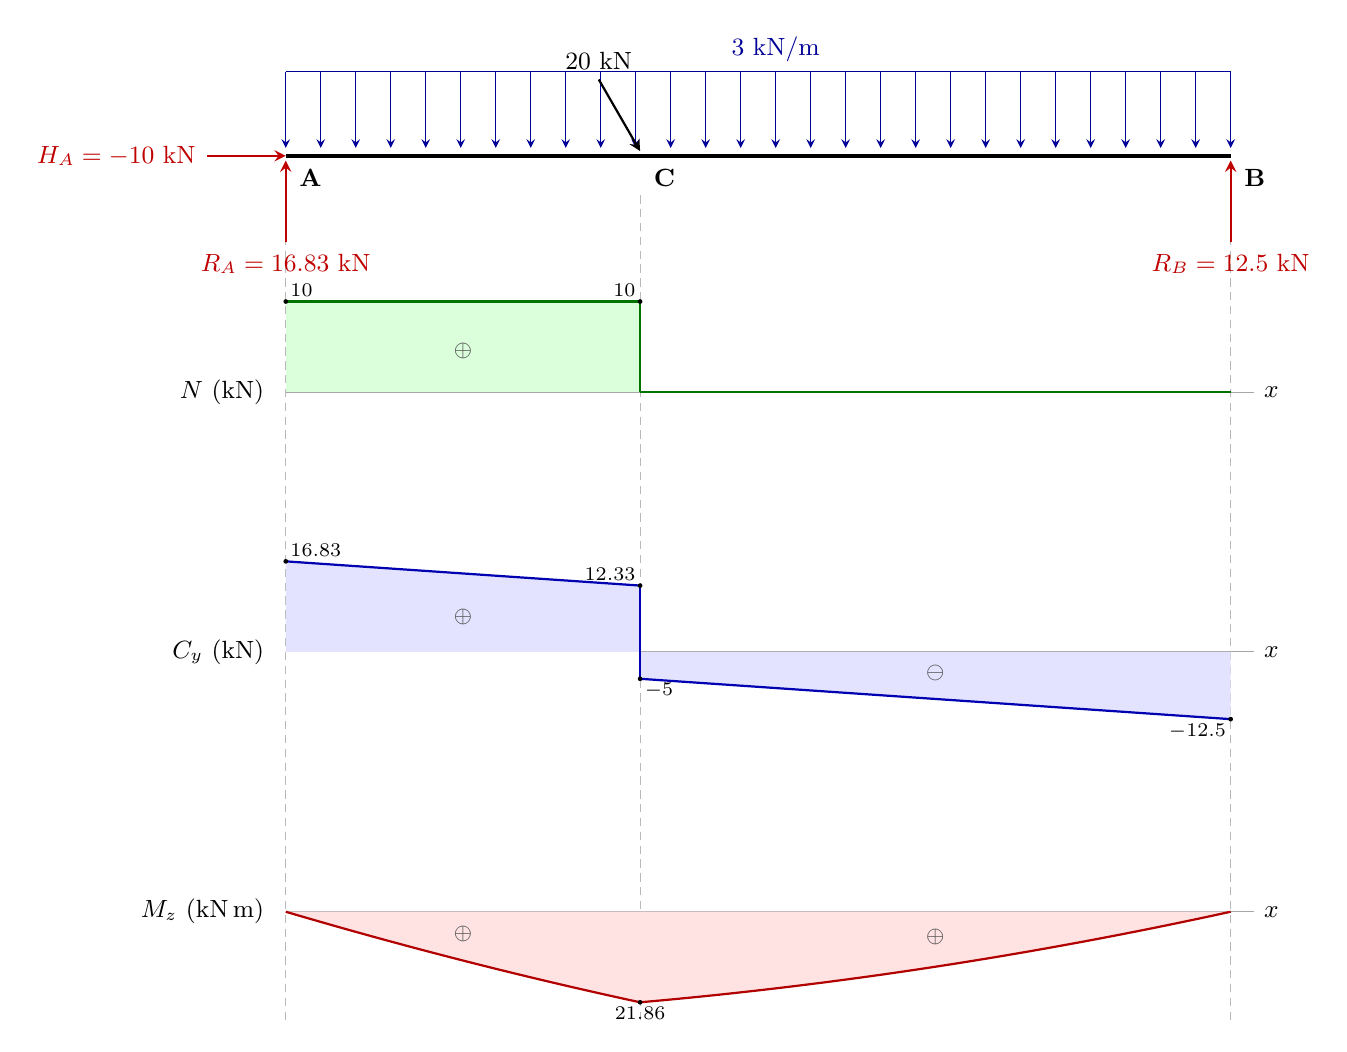
\begin{tikzpicture}
\draw[densely dashed,gray!55] (12.0000,-0.5000) -- (12.0000,-11.0000);
\draw[densely dashed,gray!55] (4.5000,-0.5000) -- (4.5000,-11.0000);
\draw[densely dashed,gray!55] (0.0000,-0.5000) -- (0.0000,-11.0000);
\draw[-stealth,blue!60!black] (0.0000,1.0700) -- (0.0000,0.1000);
\draw[-stealth,blue!60!black] (0.4444,1.0700) -- (0.4444,0.1000);
\draw[-stealth,blue!60!black] (0.8889,1.0700) -- (0.8889,0.1000);
\draw[-stealth,blue!60!black] (1.3333,1.0700) -- (1.3333,0.1000);
\draw[-stealth,blue!60!black] (1.7778,1.0700) -- (1.7778,0.1000);
\draw[-stealth,blue!60!black] (2.2222,1.0700) -- (2.2222,0.1000);
\draw[-stealth,blue!60!black] (2.6667,1.0700) -- (2.6667,0.1000);
\draw[-stealth,blue!60!black] (3.1111,1.0700) -- (3.1111,0.1000);
\draw[-stealth,blue!60!black] (3.5556,1.0700) -- (3.5556,0.1000);
\draw[-stealth,blue!60!black] (4.0000,1.0700) -- (4.0000,0.1000);
\draw[-stealth,blue!60!black] (4.4444,1.0700) -- (4.4444,0.1000);
\draw[-stealth,blue!60!black] (4.8889,1.0700) -- (4.8889,0.1000);
\draw[-stealth,blue!60!black] (5.3333,1.0700) -- (5.3333,0.1000);
\draw[-stealth,blue!60!black] (5.7778,1.0700) -- (5.7778,0.1000);
\draw[-stealth,blue!60!black] (6.2222,1.0700) -- (6.2222,0.1000);
\draw[-stealth,blue!60!black] (6.6667,1.0700) -- (6.6667,0.1000);
\draw[-stealth,blue!60!black] (7.1111,1.0700) -- (7.1111,0.1000);
\draw[-stealth,blue!60!black] (7.5556,1.0700) -- (7.5556,0.1000);
\draw[-stealth,blue!60!black] (8.0000,1.0700) -- (8.0000,0.1000);
\draw[-stealth,blue!60!black] (8.4444,1.0700) -- (8.4444,0.1000);
\draw[-stealth,blue!60!black] (8.8889,1.0700) -- (8.8889,0.1000);
\draw[-stealth,blue!60!black] (9.3333,1.0700) -- (9.3333,0.1000);
\draw[-stealth,blue!60!black] (9.7778,1.0700) -- (9.7778,0.1000);
\draw[-stealth,blue!60!black] (10.2222,1.0700) -- (10.2222,0.1000);
\draw[-stealth,blue!60!black] (10.6667,1.0700) -- (10.6667,0.1000);
\draw[-stealth,blue!60!black] (11.1111,1.0700) -- (11.1111,0.1000);
\draw[-stealth,blue!60!black] (11.5556,1.0700) -- (11.5556,0.1000);
\draw[-stealth,blue!60!black] (12.0000,1.0700) -- (12.0000,0.1000);
% studium:at distributed 0 x=0 to=4 check=span
\draw[blue!60!black] (0.0000,1.0700) -- (0.4444,1.0700) -- (0.8889,1.0700) -- (1.3333,1.0700) -- (1.7778,1.0700) -- (2.2222,1.0700) -- (2.6667,1.0700) -- (3.1111,1.0700) -- (3.5556,1.0700) -- (4.0000,1.0700) -- (4.4444,1.0700) -- (4.8889,1.0700) -- (5.3333,1.0700) -- (5.7778,1.0700) -- (6.2222,1.0700) -- (6.6667,1.0700) -- (7.1111,1.0700) -- (7.5556,1.0700) -- (8.0000,1.0700) -- (8.4444,1.0700) -- (8.8889,1.0700) -- (9.3333,1.0700) -- (9.7778,1.0700) -- (10.2222,1.0700) -- (10.6667,1.0700) -- (11.1111,1.0700) -- (11.5556,1.0700) -- (12.0000,1.0700);
\node[font=\small,anchor=south,blue!60!black] at (6.2222,1.0700) {$3$~\mbox{kN/m}};
\draw[line width=1.6pt] (0,0.0000) -- (12.0000,0.0000);
% studium:at force 0 x=3/2 check=tip
\draw[-stealth,thick,black] (3.9750,0.9693) -- (4.5000,0.0600);
\node[font=\small,anchor=south] at (3.9750,0.9693) {$20$~\mbox{kN}};
% studium:reaction H_A value=-10
% studium:at reaction H_A x=0 check=tip
\draw[-stealth,thick,red!75!black] (-1.0000,0.0000) -- (0.0000,0.0000);
\node[font=\small,anchor=east,red!75!black] at (-1.0200,0.0000) {$H_{A} = -10$~\mbox{kN}};
% studium:reaction R_A value=16.83
% studium:at reaction R_A x=0 check=tip
\draw[-stealth,thick,red!75!black] (0.0000,-1.1000) -- (0.0000,-0.0600);
\node[font=\small,anchor=north,red!75!black] at (0.0000,-1.1200) {$R_{A} = 16.83$~\mbox{kN}};
% studium:reaction R_B value=12.5
% studium:at reaction R_B x=4 check=tip
\draw[-stealth,thick,red!75!black] (12.0000,-1.1000) -- (12.0000,-0.0600);
\node[font=\small,anchor=north,red!75!black] at (12.0000,-1.1200) {$R_{B} = 12.5$~\mbox{kN}};
\node[font=\small\bfseries,anchor=north west] at (0.0500,-0.0500) {A};
\node[font=\small\bfseries,anchor=north west] at (4.5500,-0.0500) {C};
\node[font=\small\bfseries,anchor=north west] at (12.0500,-0.0500) {B};
\draw[gray!70] (0,-3.0000) -- (12.3000,-3.0000);
\fill[green!14] (0.0000,-3.0000) -- (0.0000,-1.8500) -- (4.5000,-1.8500) -- (4.5000,-3.0000) -- cycle;
\fill[green!14] (4.5000,-3.0000) -- (4.5000,-3.0000) -- (12.0000,-3.0000) -- (12.0000,-3.0000) -- cycle;
% studium:series N sx=3.0 sy=0.11499999999999999 x0=0.0 y0=-3.0 sign=1
\draw[thick,green!45!black] (0.0000,-1.8500) -- (4.5000,-1.8500);
\draw[thick,green!45!black] (4.5000,-3.0000) -- (12.0000,-3.0000);
% studium:end N
\draw[thick,green!45!black] (4.5000,-1.8500) -- (4.5000,-3.0000);
\node[font=\small,anchor=east] at (-0.15,-3.0000) {$N$ (kN)};
\node[font=\small,anchor=west] at (12.3000,-3.0000) {$x$};
% studium:label N x=0 side=right value=10
\fill (0.0000,-1.8500) circle (0.03);
\node[font=\scriptsize,anchor=south west,inner sep=1.5pt] at (0.0000,-1.8500) {$10$};
% studium:label N x=3/2 side=left value=10
\fill (4.5000,-1.8500) circle (0.03);
\node[font=\scriptsize,anchor=south east,inner sep=1.5pt] at (4.5000,-1.8500) {$10$};
\node[font=\footnotesize,gray!60!black] at (2.2500,-2.4825) {$\oplus$};
\draw[gray!70] (0,-6.3000) -- (12.3000,-6.3000);
\fill[blue!11] (0.0000,-6.3000) -- (0.0000,-5.1500) -- (4.5000,-5.4576) -- (4.5000,-6.3000) -- cycle;
\fill[blue!11] (4.5000,-6.3000) -- (4.5000,-6.6414) -- (12.0000,-7.1540) -- (12.0000,-6.3000) -- cycle;
% studium:series V sx=3.0 sy=0.06834937865313385 x0=0.0 y0=-6.3 sign=1
\draw[thick,blue!70!black] (0.0000,-5.1500) -- (4.5000,-5.4576);
\draw[thick,blue!70!black] (4.5000,-6.6414) -- (12.0000,-7.1540);
% studium:end V
\draw[thick,blue!70!black] (4.5000,-5.4576) -- (4.5000,-6.6414);
\node[font=\small,anchor=east] at (-0.15,-6.3000) {$C_y$ (kN)};
\node[font=\small,anchor=west] at (12.3000,-6.3000) {$x$};
% studium:label V x=0 side=right value=16.83
\fill (0.0000,-5.1500) circle (0.03);
\node[font=\scriptsize,anchor=south west,inner sep=1.5pt] at (0.0000,-5.1500) {$16.83$};
% studium:label V x=3/2 side=left value=12.33
\fill (4.5000,-5.4576) circle (0.03);
\node[font=\scriptsize,anchor=south east,inner sep=1.5pt] at (4.5000,-5.4576) {$12.33$};
% studium:label V x=3/2 side=right value=-5
\fill (4.5000,-6.6414) circle (0.03);
\node[font=\scriptsize,anchor=north west,inner sep=1.5pt] at (4.5000,-6.6414) {$-5$};
% studium:label V x=4 side=left value=-12.5
\fill (12.0000,-7.1540) circle (0.03);
\node[font=\scriptsize,anchor=north east,inner sep=1.5pt] at (12.0000,-7.1540) {$-12.5$};
\node[font=\footnotesize,gray!60!black] at (2.2500,-5.8517) {$\oplus$};
\node[font=\footnotesize,gray!60!black] at (8.2500,-6.5690) {$\ominus$};
\draw[gray!70] (0,-9.6000) -- (12.3000,-9.6000);
\fill[red!11] (0.0000,-9.6000) -- (0.0000,-9.6000) -- (0.1406,-9.6413) -- (0.2812,-9.6823) -- (0.4219,-9.7229) -- (0.5625,-9.7632) -- (0.7031,-9.8031) -- (0.8438,-9.8427) -- (0.9844,-9.8819) -- (1.1250,-9.9208) -- (1.2656,-9.9593) -- (1.4062,-9.9975) -- (1.5469,-10.0354) -- (1.6875,-10.0729) -- (1.8281,-10.1100) -- (1.9688,-10.1468) -- (2.1094,-10.1833) -- (2.2500,-10.2194) -- (2.3906,-10.2551) -- (2.5312,-10.2906) -- (2.6719,-10.3256) -- (2.8125,-10.3604) -- (2.9531,-10.3947) -- (3.0938,-10.4288) -- (3.2344,-10.4624) -- (3.3750,-10.4958) -- (3.5156,-10.5288) -- (3.6562,-10.5614) -- (3.7969,-10.5937) -- (3.9375,-10.6257) -- (4.0781,-10.6573) -- (4.2188,-10.6885) -- (4.3594,-10.7194) -- (4.5000,-10.7500) -- (4.5000,-9.6000) -- cycle;
\fill[red!11] (4.5000,-9.6000) -- (4.5000,-10.7500) -- (4.7344,-10.7290) -- (4.9688,-10.7070) -- (5.2031,-10.6841) -- (5.4375,-10.6602) -- (5.6719,-10.6353) -- (5.9062,-10.6095) -- (6.1406,-10.5827) -- (6.3750,-10.5550) -- (6.6094,-10.5262) -- (6.8438,-10.4966) -- (7.0781,-10.4659) -- (7.3125,-10.4343) -- (7.5469,-10.4018) -- (7.7812,-10.3682) -- (8.0156,-10.3337) -- (8.2500,-10.2983) -- (8.4844,-10.2619) -- (8.7188,-10.2245) -- (8.9531,-10.1861) -- (9.1875,-10.1468) -- (9.4219,-10.1066) -- (9.6562,-10.0653) -- (9.8906,-10.0231) -- (10.1250,-9.9800) -- (10.3594,-9.9358) -- (10.5938,-9.8907) -- (10.8281,-9.8447) -- (11.0625,-9.7977) -- (11.2969,-9.7497) -- (11.5312,-9.7008) -- (11.7656,-9.6509) -- (12.0000,-9.6000) -- (12.0000,-9.6000) -- cycle;
% studium:series M sx=3.0 sy=0.0526003405537054 x0=0.0 y0=-9.6 sign=-1
\draw[thick,red!70!black] (0.0000,-9.6000) -- (0.1406,-9.6413) -- (0.2812,-9.6823) -- (0.4219,-9.7229) -- (0.5625,-9.7632) -- (0.7031,-9.8031) -- (0.8438,-9.8427) -- (0.9844,-9.8819) -- (1.1250,-9.9208) -- (1.2656,-9.9593) -- (1.4062,-9.9975) -- (1.5469,-10.0354) -- (1.6875,-10.0729) -- (1.8281,-10.1100) -- (1.9688,-10.1468) -- (2.1094,-10.1833) -- (2.2500,-10.2194) -- (2.3906,-10.2551) -- (2.5312,-10.2906) -- (2.6719,-10.3256) -- (2.8125,-10.3604) -- (2.9531,-10.3947) -- (3.0938,-10.4288) -- (3.2344,-10.4624) -- (3.3750,-10.4958) -- (3.5156,-10.5288) -- (3.6562,-10.5614) -- (3.7969,-10.5937) -- (3.9375,-10.6257) -- (4.0781,-10.6573) -- (4.2188,-10.6885) -- (4.3594,-10.7194) -- (4.5000,-10.7500);
\draw[thick,red!70!black] (4.5000,-10.7500) -- (4.7344,-10.7290) -- (4.9688,-10.7070) -- (5.2031,-10.6841) -- (5.4375,-10.6602) -- (5.6719,-10.6353) -- (5.9062,-10.6095) -- (6.1406,-10.5827) -- (6.3750,-10.5550) -- (6.6094,-10.5262) -- (6.8438,-10.4966) -- (7.0781,-10.4659) -- (7.3125,-10.4343) -- (7.5469,-10.4018) -- (7.7812,-10.3682) -- (8.0156,-10.3337) -- (8.2500,-10.2983) -- (8.4844,-10.2619) -- (8.7188,-10.2245) -- (8.9531,-10.1861) -- (9.1875,-10.1468) -- (9.4219,-10.1066) -- (9.6562,-10.0653) -- (9.8906,-10.0231) -- (10.1250,-9.9800) -- (10.3594,-9.9358) -- (10.5938,-9.8907) -- (10.8281,-9.8447) -- (11.0625,-9.7977) -- (11.2969,-9.7497) -- (11.5312,-9.7008) -- (11.7656,-9.6509) -- (12.0000,-9.6000);
% studium:end M
\node[font=\small,anchor=east] at (-0.15,-9.6000) {$M_z$ (kN\,m)};
\node[font=\small,anchor=west] at (12.3000,-9.6000) {$x$};
% studium:label M x=3/2 side=both value=21.86
\fill (4.5000,-10.7500) circle (0.03);
\node[font=\scriptsize,anchor=north,inner sep=1.5pt] at (4.5000,-10.7500) {$21.86$};
\node[font=\footnotesize,gray!60!black] at (2.2500,-9.8787) {$\oplus$};
\node[font=\footnotesize,gray!60!black] at (8.2500,-9.9142) {$\oplus$};
\end{tikzpicture}}%
\else
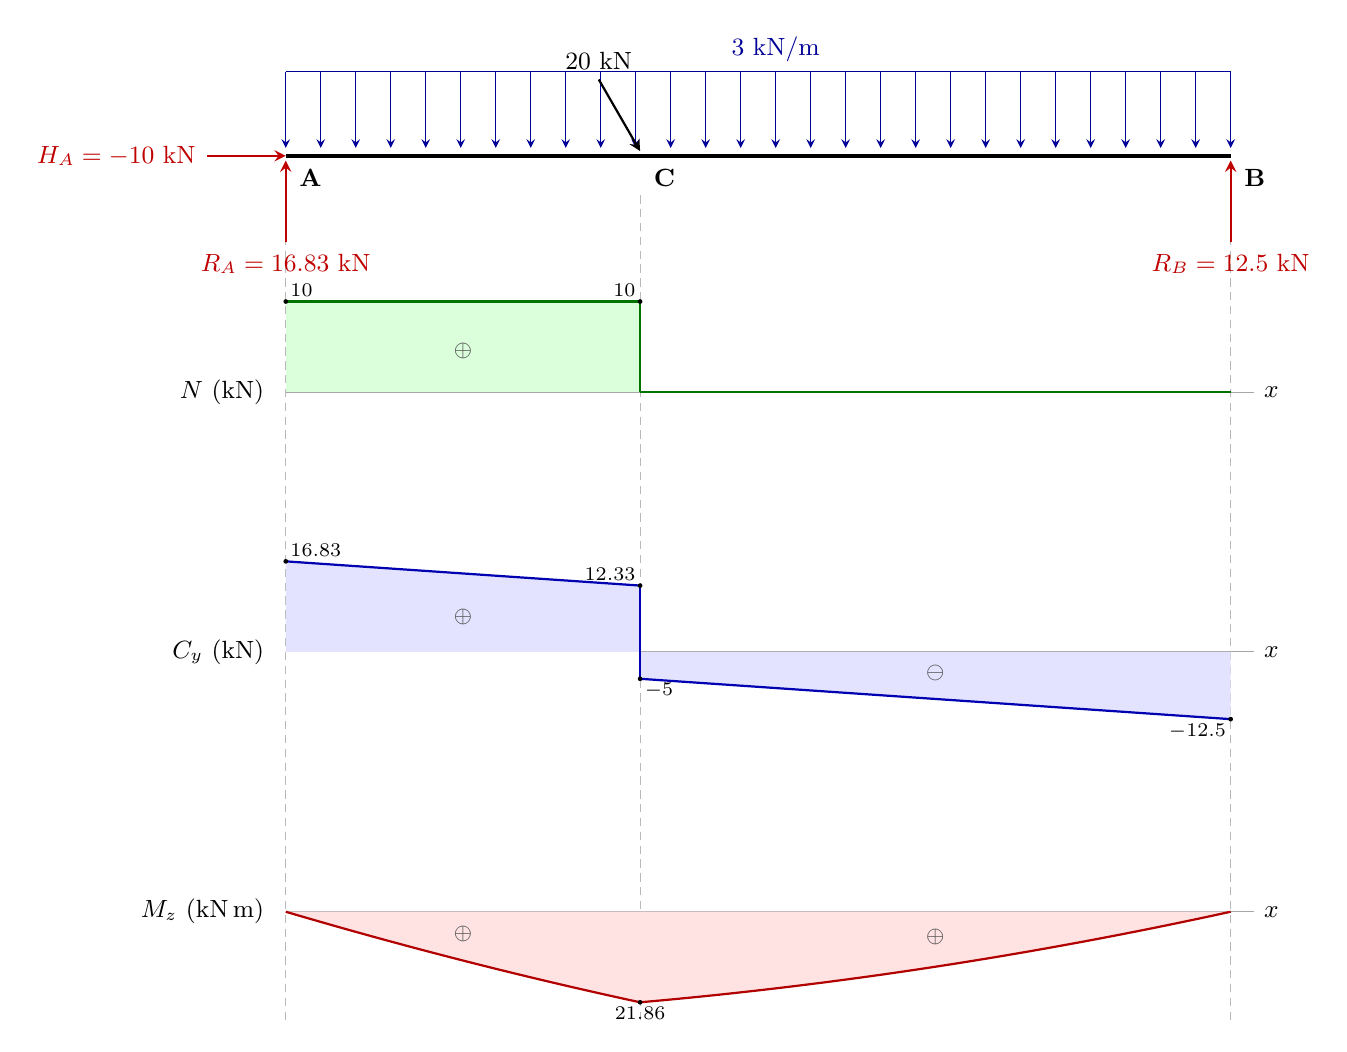
\begin{tikzpicture}
\draw[densely dashed,gray!55] (12.0000,-0.5000) -- (12.0000,-11.0000);
\draw[densely dashed,gray!55] (4.5000,-0.5000) -- (4.5000,-11.0000);
\draw[densely dashed,gray!55] (0.0000,-0.5000) -- (0.0000,-11.0000);
\draw[-stealth,blue!60!black] (0.0000,1.0700) -- (0.0000,0.1000);
\draw[-stealth,blue!60!black] (0.4444,1.0700) -- (0.4444,0.1000);
\draw[-stealth,blue!60!black] (0.8889,1.0700) -- (0.8889,0.1000);
\draw[-stealth,blue!60!black] (1.3333,1.0700) -- (1.3333,0.1000);
\draw[-stealth,blue!60!black] (1.7778,1.0700) -- (1.7778,0.1000);
\draw[-stealth,blue!60!black] (2.2222,1.0700) -- (2.2222,0.1000);
\draw[-stealth,blue!60!black] (2.6667,1.0700) -- (2.6667,0.1000);
\draw[-stealth,blue!60!black] (3.1111,1.0700) -- (3.1111,0.1000);
\draw[-stealth,blue!60!black] (3.5556,1.0700) -- (3.5556,0.1000);
\draw[-stealth,blue!60!black] (4.0000,1.0700) -- (4.0000,0.1000);
\draw[-stealth,blue!60!black] (4.4444,1.0700) -- (4.4444,0.1000);
\draw[-stealth,blue!60!black] (4.8889,1.0700) -- (4.8889,0.1000);
\draw[-stealth,blue!60!black] (5.3333,1.0700) -- (5.3333,0.1000);
\draw[-stealth,blue!60!black] (5.7778,1.0700) -- (5.7778,0.1000);
\draw[-stealth,blue!60!black] (6.2222,1.0700) -- (6.2222,0.1000);
\draw[-stealth,blue!60!black] (6.6667,1.0700) -- (6.6667,0.1000);
\draw[-stealth,blue!60!black] (7.1111,1.0700) -- (7.1111,0.1000);
\draw[-stealth,blue!60!black] (7.5556,1.0700) -- (7.5556,0.1000);
\draw[-stealth,blue!60!black] (8.0000,1.0700) -- (8.0000,0.1000);
\draw[-stealth,blue!60!black] (8.4444,1.0700) -- (8.4444,0.1000);
\draw[-stealth,blue!60!black] (8.8889,1.0700) -- (8.8889,0.1000);
\draw[-stealth,blue!60!black] (9.3333,1.0700) -- (9.3333,0.1000);
\draw[-stealth,blue!60!black] (9.7778,1.0700) -- (9.7778,0.1000);
\draw[-stealth,blue!60!black] (10.2222,1.0700) -- (10.2222,0.1000);
\draw[-stealth,blue!60!black] (10.6667,1.0700) -- (10.6667,0.1000);
\draw[-stealth,blue!60!black] (11.1111,1.0700) -- (11.1111,0.1000);
\draw[-stealth,blue!60!black] (11.5556,1.0700) -- (11.5556,0.1000);
\draw[-stealth,blue!60!black] (12.0000,1.0700) -- (12.0000,0.1000);
% studium:at distributed 0 x=0 to=4 check=span
\draw[blue!60!black] (0.0000,1.0700) -- (0.4444,1.0700) -- (0.8889,1.0700) -- (1.3333,1.0700) -- (1.7778,1.0700) -- (2.2222,1.0700) -- (2.6667,1.0700) -- (3.1111,1.0700) -- (3.5556,1.0700) -- (4.0000,1.0700) -- (4.4444,1.0700) -- (4.8889,1.0700) -- (5.3333,1.0700) -- (5.7778,1.0700) -- (6.2222,1.0700) -- (6.6667,1.0700) -- (7.1111,1.0700) -- (7.5556,1.0700) -- (8.0000,1.0700) -- (8.4444,1.0700) -- (8.8889,1.0700) -- (9.3333,1.0700) -- (9.7778,1.0700) -- (10.2222,1.0700) -- (10.6667,1.0700) -- (11.1111,1.0700) -- (11.5556,1.0700) -- (12.0000,1.0700);
\node[font=\small,anchor=south,blue!60!black] at (6.2222,1.0700) {$3$~\mbox{kN/m}};
\draw[line width=1.6pt] (0,0.0000) -- (12.0000,0.0000);
% studium:at force 0 x=3/2 check=tip
\draw[-stealth,thick,black] (3.9750,0.9693) -- (4.5000,0.0600);
\node[font=\small,anchor=south] at (3.9750,0.9693) {$20$~\mbox{kN}};
% studium:reaction H_A value=-10
% studium:at reaction H_A x=0 check=tip
\draw[-stealth,thick,red!75!black] (-1.0000,0.0000) -- (0.0000,0.0000);
\node[font=\small,anchor=east,red!75!black] at (-1.0200,0.0000) {$H_{A} = -10$~\mbox{kN}};
% studium:reaction R_A value=16.83
% studium:at reaction R_A x=0 check=tip
\draw[-stealth,thick,red!75!black] (0.0000,-1.1000) -- (0.0000,-0.0600);
\node[font=\small,anchor=north,red!75!black] at (0.0000,-1.1200) {$R_{A} = 16.83$~\mbox{kN}};
% studium:reaction R_B value=12.5
% studium:at reaction R_B x=4 check=tip
\draw[-stealth,thick,red!75!black] (12.0000,-1.1000) -- (12.0000,-0.0600);
\node[font=\small,anchor=north,red!75!black] at (12.0000,-1.1200) {$R_{B} = 12.5$~\mbox{kN}};
\node[font=\small\bfseries,anchor=north west] at (0.0500,-0.0500) {A};
\node[font=\small\bfseries,anchor=north west] at (4.5500,-0.0500) {C};
\node[font=\small\bfseries,anchor=north west] at (12.0500,-0.0500) {B};
\draw[gray!70] (0,-3.0000) -- (12.3000,-3.0000);
\fill[green!14] (0.0000,-3.0000) -- (0.0000,-1.8500) -- (4.5000,-1.8500) -- (4.5000,-3.0000) -- cycle;
\fill[green!14] (4.5000,-3.0000) -- (4.5000,-3.0000) -- (12.0000,-3.0000) -- (12.0000,-3.0000) -- cycle;
% studium:series N sx=3.0 sy=0.11499999999999999 x0=0.0 y0=-3.0 sign=1
\draw[thick,green!45!black] (0.0000,-1.8500) -- (4.5000,-1.8500);
\draw[thick,green!45!black] (4.5000,-3.0000) -- (12.0000,-3.0000);
% studium:end N
\draw[thick,green!45!black] (4.5000,-1.8500) -- (4.5000,-3.0000);
\node[font=\small,anchor=east] at (-0.15,-3.0000) {$N$ (kN)};
\node[font=\small,anchor=west] at (12.3000,-3.0000) {$x$};
% studium:label N x=0 side=right value=10
\fill (0.0000,-1.8500) circle (0.03);
\node[font=\scriptsize,anchor=south west,inner sep=1.5pt] at (0.0000,-1.8500) {$10$};
% studium:label N x=3/2 side=left value=10
\fill (4.5000,-1.8500) circle (0.03);
\node[font=\scriptsize,anchor=south east,inner sep=1.5pt] at (4.5000,-1.8500) {$10$};
\node[font=\footnotesize,gray!60!black] at (2.2500,-2.4825) {$\oplus$};
\draw[gray!70] (0,-6.3000) -- (12.3000,-6.3000);
\fill[blue!11] (0.0000,-6.3000) -- (0.0000,-5.1500) -- (4.5000,-5.4576) -- (4.5000,-6.3000) -- cycle;
\fill[blue!11] (4.5000,-6.3000) -- (4.5000,-6.6414) -- (12.0000,-7.1540) -- (12.0000,-6.3000) -- cycle;
% studium:series V sx=3.0 sy=0.06834937865313385 x0=0.0 y0=-6.3 sign=1
\draw[thick,blue!70!black] (0.0000,-5.1500) -- (4.5000,-5.4576);
\draw[thick,blue!70!black] (4.5000,-6.6414) -- (12.0000,-7.1540);
% studium:end V
\draw[thick,blue!70!black] (4.5000,-5.4576) -- (4.5000,-6.6414);
\node[font=\small,anchor=east] at (-0.15,-6.3000) {$C_y$ (kN)};
\node[font=\small,anchor=west] at (12.3000,-6.3000) {$x$};
% studium:label V x=0 side=right value=16.83
\fill (0.0000,-5.1500) circle (0.03);
\node[font=\scriptsize,anchor=south west,inner sep=1.5pt] at (0.0000,-5.1500) {$16.83$};
% studium:label V x=3/2 side=left value=12.33
\fill (4.5000,-5.4576) circle (0.03);
\node[font=\scriptsize,anchor=south east,inner sep=1.5pt] at (4.5000,-5.4576) {$12.33$};
% studium:label V x=3/2 side=right value=-5
\fill (4.5000,-6.6414) circle (0.03);
\node[font=\scriptsize,anchor=north west,inner sep=1.5pt] at (4.5000,-6.6414) {$-5$};
% studium:label V x=4 side=left value=-12.5
\fill (12.0000,-7.1540) circle (0.03);
\node[font=\scriptsize,anchor=north east,inner sep=1.5pt] at (12.0000,-7.1540) {$-12.5$};
\node[font=\footnotesize,gray!60!black] at (2.2500,-5.8517) {$\oplus$};
\node[font=\footnotesize,gray!60!black] at (8.2500,-6.5690) {$\ominus$};
\draw[gray!70] (0,-9.6000) -- (12.3000,-9.6000);
\fill[red!11] (0.0000,-9.6000) -- (0.0000,-9.6000) -- (0.1406,-9.6413) -- (0.2812,-9.6823) -- (0.4219,-9.7229) -- (0.5625,-9.7632) -- (0.7031,-9.8031) -- (0.8438,-9.8427) -- (0.9844,-9.8819) -- (1.1250,-9.9208) -- (1.2656,-9.9593) -- (1.4062,-9.9975) -- (1.5469,-10.0354) -- (1.6875,-10.0729) -- (1.8281,-10.1100) -- (1.9688,-10.1468) -- (2.1094,-10.1833) -- (2.2500,-10.2194) -- (2.3906,-10.2551) -- (2.5312,-10.2906) -- (2.6719,-10.3256) -- (2.8125,-10.3604) -- (2.9531,-10.3947) -- (3.0938,-10.4288) -- (3.2344,-10.4624) -- (3.3750,-10.4958) -- (3.5156,-10.5288) -- (3.6562,-10.5614) -- (3.7969,-10.5937) -- (3.9375,-10.6257) -- (4.0781,-10.6573) -- (4.2188,-10.6885) -- (4.3594,-10.7194) -- (4.5000,-10.7500) -- (4.5000,-9.6000) -- cycle;
\fill[red!11] (4.5000,-9.6000) -- (4.5000,-10.7500) -- (4.7344,-10.7290) -- (4.9688,-10.7070) -- (5.2031,-10.6841) -- (5.4375,-10.6602) -- (5.6719,-10.6353) -- (5.9062,-10.6095) -- (6.1406,-10.5827) -- (6.3750,-10.5550) -- (6.6094,-10.5262) -- (6.8438,-10.4966) -- (7.0781,-10.4659) -- (7.3125,-10.4343) -- (7.5469,-10.4018) -- (7.7812,-10.3682) -- (8.0156,-10.3337) -- (8.2500,-10.2983) -- (8.4844,-10.2619) -- (8.7188,-10.2245) -- (8.9531,-10.1861) -- (9.1875,-10.1468) -- (9.4219,-10.1066) -- (9.6562,-10.0653) -- (9.8906,-10.0231) -- (10.1250,-9.9800) -- (10.3594,-9.9358) -- (10.5938,-9.8907) -- (10.8281,-9.8447) -- (11.0625,-9.7977) -- (11.2969,-9.7497) -- (11.5312,-9.7008) -- (11.7656,-9.6509) -- (12.0000,-9.6000) -- (12.0000,-9.6000) -- cycle;
% studium:series M sx=3.0 sy=0.0526003405537054 x0=0.0 y0=-9.6 sign=-1
\draw[thick,red!70!black] (0.0000,-9.6000) -- (0.1406,-9.6413) -- (0.2812,-9.6823) -- (0.4219,-9.7229) -- (0.5625,-9.7632) -- (0.7031,-9.8031) -- (0.8438,-9.8427) -- (0.9844,-9.8819) -- (1.1250,-9.9208) -- (1.2656,-9.9593) -- (1.4062,-9.9975) -- (1.5469,-10.0354) -- (1.6875,-10.0729) -- (1.8281,-10.1100) -- (1.9688,-10.1468) -- (2.1094,-10.1833) -- (2.2500,-10.2194) -- (2.3906,-10.2551) -- (2.5312,-10.2906) -- (2.6719,-10.3256) -- (2.8125,-10.3604) -- (2.9531,-10.3947) -- (3.0938,-10.4288) -- (3.2344,-10.4624) -- (3.3750,-10.4958) -- (3.5156,-10.5288) -- (3.6562,-10.5614) -- (3.7969,-10.5937) -- (3.9375,-10.6257) -- (4.0781,-10.6573) -- (4.2188,-10.6885) -- (4.3594,-10.7194) -- (4.5000,-10.7500);
\draw[thick,red!70!black] (4.5000,-10.7500) -- (4.7344,-10.7290) -- (4.9688,-10.7070) -- (5.2031,-10.6841) -- (5.4375,-10.6602) -- (5.6719,-10.6353) -- (5.9062,-10.6095) -- (6.1406,-10.5827) -- (6.3750,-10.5550) -- (6.6094,-10.5262) -- (6.8438,-10.4966) -- (7.0781,-10.4659) -- (7.3125,-10.4343) -- (7.5469,-10.4018) -- (7.7812,-10.3682) -- (8.0156,-10.3337) -- (8.2500,-10.2983) -- (8.4844,-10.2619) -- (8.7188,-10.2245) -- (8.9531,-10.1861) -- (9.1875,-10.1468) -- (9.4219,-10.1066) -- (9.6562,-10.0653) -- (9.8906,-10.0231) -- (10.1250,-9.9800) -- (10.3594,-9.9358) -- (10.5938,-9.8907) -- (10.8281,-9.8447) -- (11.0625,-9.7977) -- (11.2969,-9.7497) -- (11.5312,-9.7008) -- (11.7656,-9.6509) -- (12.0000,-9.6000);
% studium:end M
\node[font=\small,anchor=east] at (-0.15,-9.6000) {$M_z$ (kN\,m)};
\node[font=\small,anchor=west] at (12.3000,-9.6000) {$x$};
% studium:label M x=3/2 side=both value=21.86
\fill (4.5000,-10.7500) circle (0.03);
\node[font=\scriptsize,anchor=north,inner sep=1.5pt] at (4.5000,-10.7500) {$21.86$};
\node[font=\footnotesize,gray!60!black] at (2.2500,-9.8787) {$\oplus$};
\node[font=\footnotesize,gray!60!black] at (8.2500,-9.9142) {$\oplus$};
\end{tikzpicture}%
\fi
\fi
\endgroup
\par\nopagebreak
\studiumcaption{fig:e2-c03-incl-esfuerzos}{Axiles, cortantes y flectores: el axil solo existe entre el apoyo fijo y el punto de aplicación de la fuerza.}
\end{minipage}\par\medskip

\textbf{Resultado e interpretación.}\[\fitmath{N_{AC} = 10\ \mathrm{kN},\quad N_{CB} = 0,\quad M_{z,\max} = 21.86\ \mathrm{kN\,m}\ (x = 1.5\ \mathrm{m})}\]

La fuerza inclinada hace trabajar a la viga a la vez en tracción y en flexión. El axil es constante a trozos porque no hay cargas axiales repartidas, y se anula a la derecha de $C$ porque el apoyo móvil no ejerce fuerza horizontal.

\par\textbf{Comprobación.} Recalcula los pasos con unidades coherentes y aplica el control específico indicado en la orientación del capítulo.

\textbf{Límites.}\begin{itemize}\item no se considera la excentricidad de la fuerza respecto a la directriz\end{itemize}

\textbf{Errores frecuentes.}\begin{itemize}\item repartir la componente horizontal entre los dos apoyos
\item olvidar la componente vertical de la fuerza inclinada en el equilibrio de momentos\end{itemize}

\end{studiumworked}

\Needspace{.3\textheight}

\begin{studiumworked}{PRB-0187}

\section{PRB-0187 · Flector en el empotramiento}

\textbf{Enunciado.} Una ménsula de 2 m de longitud, empotrada en su extremo izquierdo, soporta una carga puntual de 10 kN hacia abajo en su extremo libre. Calcule el flector en el empotramiento con el criterio de signos del curso (positivo si comprime la fibra superior).

\par\medskip\noindent\begin{tabular}{@{}p{.18\linewidth}p{.26\linewidth}p{.48\linewidth}@{}}
\toprule Símbolo & Valor y unidad & Significado\\\midrule
$P$ & $10\,\mathrm{kN}$ & carga en el extremo\\
$L$ & $2\,\mathrm{m}$ & longitud\\
\bottomrule\end{tabular}\par\medskip

\textbf{Hipótesis.}\begin{itemize}\item ménsula empotrada en x = 0
\item carga hacia abajo\end{itemize}

\textbf{Modelo y desarrollo.}

Flector de una ménsula con carga en el extremo.\[\fitmath{M_z(0) = -P\,L}\]

\textbf{Procedimiento.}\begin{itemize}\item En una sección de abscisa $x$ el flector es $M_z(x) = -P(L - x)$, negativo, porque la carga tracciona las fibras superiores.
\item En $x = 0$ resulta $-PL$.\end{itemize}

\textbf{Cálculo de los pasos.}

\begin{enumerate}

\item Flector en el empotramiento.

\[\fitmath{y_{1}=-10\cdot 2\approx -20\,\mathrm{kN m}}\]

\end{enumerate}

\textbf{Resultado e interpretación.}\[\fitmath{M_z(0) = -20.0\ \mathrm{kN\,m}}\]

El signo negativo indica que el empotramiento comprime la fibra inferior y tracciona la superior; el diagrama se dibuja hacia arriba.

\par\textbf{Comprobación.} Recalcula los pasos con unidades coherentes y aplica el control específico indicado en la orientación del capítulo.

\textbf{Límites.}\begin{itemize}\item no incluye el peso propio\end{itemize}

\textbf{Errores frecuentes.}\begin{itemize}\item dar el flector en valor absoluto sin signo\end{itemize}

\end{studiumworked}

\Needspace{.3\textheight}

\begin{studiumworked}{PRB-0188}

\section{PRB-0188 · Flector máximo}

\textbf{Enunciado.} Una viga biapoyada de 5 m de luz soporta una carga puntual de 20 kN en el centro. Calcule el momento flector máximo.

\par\medskip\noindent\begin{tabular}{@{}p{.18\linewidth}p{.26\linewidth}p{.48\linewidth}@{}}
\toprule Símbolo & Valor y unidad & Significado\\\midrule
$P$ & $20\,\mathrm{kN}$ & carga central\\
$L$ & $5\,\mathrm{m}$ & luz\\
\bottomrule\end{tabular}\par\medskip

\textbf{Hipótesis.}\begin{itemize}\item viga biapoyada isostática\end{itemize}

\textbf{Modelo y desarrollo.}

Flector máximo con carga central.\[\fitmath{M_{max} = \frac{P\,L}{4}}\]

\textbf{Procedimiento.}\begin{itemize}\item Cada reacción vale $P/2 = 10$ kN.
\item El flector en el centro es $R_A\,L/2 = P L/4$.\end{itemize}

\textbf{Cálculo de los pasos.}

\begin{enumerate}

\item Flector máximo.

\[\fitmath{y_{1}=\frac{20\cdot 5}{4}\approx 25\,\mathrm{kN m}}\]

\end{enumerate}

\textbf{Resultado e interpretación.}\[\fitmath{M_{max} = 25.0\ \mathrm{kN\,m}}\]

El máximo está bajo la carga, donde el cortante cambia de signo.

\par\textbf{Comprobación.} Recalcula los pasos con unidades coherentes y aplica el control específico indicado en la orientación del capítulo.

\textbf{Límites.}\begin{itemize}\item no incluye el peso propio\end{itemize}

\textbf{Errores frecuentes.}\begin{itemize}\item usar PL/2 en lugar de PL/4\end{itemize}

\end{studiumworked}

\Needspace{.3\textheight}

\begin{studiumworked}{PRB-0189}

\section{PRB-0189 · Momento de inercia}

\textbf{Enunciado.} Calcule el momento de inercia respecto al eje horizontal por el centro de gravedad de una sección rectangular de 50 mm de ancho y 120 mm de alto.

\par\medskip\noindent\begin{tabular}{@{}p{.18\linewidth}p{.26\linewidth}p{.48\linewidth}@{}}
\toprule Símbolo & Valor y unidad & Significado\\\midrule
$b$ & $50\,\mathrm{mm}$ & ancho\\
$h$ & $120\,\mathrm{mm}$ & alto\\
\bottomrule\end{tabular}\par\medskip

\textbf{Hipótesis.}\begin{itemize}\item rectángulo macizo\end{itemize}

\textbf{Modelo y desarrollo.}

Inercia de un rectángulo.\[\fitmath{I_z = \frac{b\,h^{3}}{12}}\]

\textbf{Elección del procedimiento.} La inercia respecto al eje horizontal es $I_z=\int_A y^2dA=b\int_{-h/2}^{h/2}y^2dy=bh^3/12$. La dimensión perpendicular al eje es la que aparece al cubo.

\textbf{Procedimiento.}\begin{itemize}\item La altura es la dimensión perpendicular al eje, y entra al cubo.\end{itemize}

\textbf{Cálculo de los pasos.}

\begin{enumerate}

\item Momento de inercia.

\[\fitmath{y_{1}=\frac{50\cdot {120}^{3}}{12}\approx 7200000\,\mathrm{mm^{4}}}\]

\end{enumerate}

\textbf{Resultado e interpretación.}\[\fitmath{I_z = 7.2\times 10^{6}\ \mathrm{mm}^{4}}\]

Girando la sección 90 grados la inercia sería $120\cdot 50^3/12 = 1.25\times 10^6$ mm$^4$, casi seis veces menor.

\par\textbf{Comprobación.} Recalcula los pasos con unidades coherentes y aplica el control específico indicado en la orientación del capítulo.

\textbf{Límites.}\begin{itemize}\item solo rectángulos\end{itemize}

\textbf{Errores frecuentes.}\begin{itemize}\item usar la dimensión paralela al eje elevada al cubo\end{itemize}

\end{studiumworked}

\Needspace{.3\textheight}

\begin{studiumworked}{PRB-0190}

\section{PRB-0190 · Reacción en b}

\textbf{Enunciado.} Una viga biapoyada de 4 m de luz soporta una carga triangular que vale cero en el apoyo izquierdo $A$ y 9 kN/m en el derecho $B$. Calcule la reacción en $B$.

\par\medskip\noindent\begin{tabular}{@{}p{.18\linewidth}p{.26\linewidth}p{.48\linewidth}@{}}
\toprule Símbolo & Valor y unidad & Significado\\\midrule
$L$ & $4\,\mathrm{m}$ & luz\\
$q_{0}$ & $9\,\mathrm{kN/m}$ & carga máxima\\
\bottomrule\end{tabular}\par\medskip

\textbf{Hipótesis.}\begin{itemize}\item viga isostática biapoyada\end{itemize}

\textbf{Modelo y desarrollo.}

Reacción por carga triangular.\[\fitmath{R_B = \frac{Q\cdot 2L/3}{L} = \frac{q_0\,L}{3}}\]

\textbf{Procedimiento.}\begin{itemize}\item La resultante es $Q = q_0 L/2 = 18$ kN, aplicada a $2L/3$ de $A$.
\item Momentos respecto a $A$: $R_B L = Q\cdot 2L/3$.\end{itemize}

\textbf{Cálculo de los pasos.}

\begin{enumerate}

\item Resultante de la carga.

\[\fitmath{y_{1}=\frac{9\cdot 4}{2}\approx 18\,\mathrm{kN}}\]

\item Reacción en B.

\[\fitmath{y_{2}=\frac{18\cdot \frac{2\cdot 4}{3}}{4}\approx 12\,\mathrm{kN}}\]

\end{enumerate}

\textbf{Resultado e interpretación.}\[\fitmath{R_B = 12.0\ \mathrm{kN},\qquad R_A = 6.0\ \mathrm{kN}}\]

El apoyo del lado de mayor carga recoge dos tercios de la resultante.

\par\textbf{Comprobación.} Recalcula los pasos con unidades coherentes y aplica el control específico indicado en la orientación del capítulo.

\textbf{Límites.}\begin{itemize}\item no incluye el peso propio\end{itemize}

\textbf{Errores frecuentes.}\begin{itemize}\item aplicar la resultante en el centro de la luz\end{itemize}

\end{studiumworked}

\Needspace{.3\textheight}

\begin{studiumworked}{PRB-0191}

\section{PRB-0191 · Momento de inercia respecto a la base}

\textbf{Enunciado.} Calcule el momento de inercia de un rectángulo de 40 mm de ancho y 100 mm de alto respecto al eje horizontal que pasa por su base.

\par\medskip\noindent\begin{tabular}{@{}p{.18\linewidth}p{.26\linewidth}p{.48\linewidth}@{}}
\toprule Símbolo & Valor y unidad & Significado\\\midrule
$b$ & $40\,\mathrm{mm}$ & ancho\\
$h$ & $100\,\mathrm{mm}$ & alto\\
\bottomrule\end{tabular}\par\medskip

\textbf{Hipótesis.}\begin{itemize}\item rectángulo macizo\end{itemize}

\textbf{Modelo y desarrollo.}

Steiner para un rectángulo.\[\fitmath{I_{z'} = \frac{b\,h^{3}}{12} + b\,h\left(\frac{h}{2}\right)^{2} = \frac{b\,h^{3}}{3}}\]

\textbf{Procedimiento.}\begin{itemize}\item La inercia centroidal es $bh^3/12$.
\item La distancia entre el eje centroidal y la base es $h/2$.\end{itemize}

\textbf{Cálculo de los pasos.}

\begin{enumerate}

\item Momento de inercia respecto a la base.

\[\fitmath{y_{1}=\frac{40\cdot {100}^{3}}{12}+40\cdot 100\cdot {\left(\frac{100}{2}\right)}^{2}\approx 1.333333\times10^{7}\,\mathrm{mm^{4}}}\]

\end{enumerate}

\textbf{Resultado e interpretación.}\[\fitmath{I_{z'} = 1.333\times 10^{7}\ \mathrm{mm}^{4}}\]

Coincide con $bh^3/3$, cuatro veces la inercia centroidal.

\par\textbf{Comprobación.} Recalcula los pasos con unidades coherentes y aplica el control específico indicado en la orientación del capítulo.

\textbf{Límites.}\begin{itemize}\item solo rectángulos\end{itemize}

\textbf{Errores frecuentes.}\begin{itemize}\item usar $d = h$ en lugar de $d = h/2$\end{itemize}

\end{studiumworked}

\Needspace{.3\textheight}

\begin{studiumworked}{PRB-0192}

\section{PRB-0192 · Flector máximo}

\textbf{Enunciado.} Una viga biapoyada de 5 m soporta dos cargas puntuales hacia abajo: 10 kN a 1 m del apoyo izquierdo $A$ y 20 kN a 3 m. Dibuje los diagramas de cortantes y flectores y calcule el flector máximo.

\par\medskip\noindent\begin{tabular}{@{}p{.18\linewidth}p{.26\linewidth}p{.48\linewidth}@{}}
\toprule Símbolo & Valor y unidad & Significado\\\midrule
$L$ & $5\,\mathrm{m}$ & luz\\
\bottomrule\end{tabular}\par\medskip

\textbf{Hipótesis.}\begin{itemize}\item criterio de signos del curso\end{itemize}

\textbf{Modelo y desarrollo.}

Equilibrio de la viga.\[\fitmath{\sum F_y = 0,\qquad \sum M = 0}\]

\textbf{Cálculo de los pasos.}

\begin{enumerate}

\item Reacción en B.

\[\fitmath{y_{1}=\frac{10\cdot 1+20\cdot 3}{5}\approx 14\,\mathrm{kN}}\]

\item Reacción en A.

\[\fitmath{y_{2}=30-14\approx 16\,\mathrm{kN}}\]

\item Flector máximo, bajo la carga de 20 kN.

\[\fitmath{y_{3}=14\cdot 2\approx 28\,\mathrm{kN m}}\]

\end{enumerate}

\textbf{Resultado e interpretación.}\[\fitmath{M_{z,\max} = 28\ \mathrm{kN\,m}\ (x = 3\ \mathrm{m})}\]

Sin cargas repartidas el cortante es constante entre cargas y el flector es lineal; el máximo está bajo la carga en la que el cortante pasa de positivo a negativo.

\par\textbf{Comprobación.} Recalcula los pasos con unidades coherentes y aplica el control específico indicado en la orientación del capítulo.

\textbf{Límites.}\begin{itemize}\item no se incluye el peso propio\end{itemize}

\textbf{Errores frecuentes.}\begin{itemize}\item buscar el máximo en el centro de la luz\end{itemize}

\end{studiumworked}

\Needspace{.3\textheight}

\begin{studiumworked}{PRB-0193}

\section{PRB-0193 · Flector en el empotramiento}

\textbf{Enunciado.} Una ménsula de 4 m empotrada en $A$ soporta una carga uniforme de 5 kN/m hacia abajo en su mitad exterior y una carga puntual de 4 kN hacia abajo en el centro. Escriba las leyes de esfuerzos por tramos, dibuje los diagramas y calcule el flector en el empotramiento.

\par\medskip\noindent\begin{tabular}{@{}p{.18\linewidth}p{.26\linewidth}p{.48\linewidth}@{}}
\toprule Símbolo & Valor y unidad & Significado\\\midrule
$q$ & $5\,\mathrm{kN/m}$ & carga repartida\\
\bottomrule\end{tabular}\par\medskip

\textbf{Hipótesis.}\begin{itemize}\item criterio de signos del curso\end{itemize}

\textbf{Modelo y desarrollo.}

Equilibrio de la viga.\[\fitmath{\sum F_y = 0,\qquad \sum M = 0}\]

\textbf{Cálculo de los pasos.}

\begin{enumerate}

\item Reacción vertical en A.

\[\fitmath{y_{1}=5\cdot 2+4\approx 14\,\mathrm{kN}}\]

\item Flector en el empotramiento.

\[\fitmath{y_{2}=-\left(5\cdot 2\cdot 3+4\cdot 2\right)\approx -38\,\mathrm{kN m}}\]

\end{enumerate}

\textbf{Resultado e interpretación.}\[\fitmath{M_z(0) = -38\ \mathrm{kN\,m}}\]

Toda la ménsula trabaja con la fibra superior traccionada; el flector crece en valor absoluto hacia el empotramiento, primero de forma parabólica y después lineal.

\par\textbf{Comprobación.} Recalcula los pasos con unidades coherentes y aplica el control específico indicado en la orientación del capítulo.

\textbf{Límites.}\begin{itemize}\item no se incluye el peso propio\end{itemize}

\textbf{Errores frecuentes.}\begin{itemize}\item olvidar el tramo sin carga repartida al escribir las leyes\end{itemize}

\end{studiumworked}

\Needspace{.3\textheight}

\begin{studiumworked}{PRB-0194}

\section{PRB-0194 · Reacciones y flector sobre b}

\textbf{Enunciado.} Una viga de 6 m con apoyo fijo en $A$ y apoyo móvil en $B$, a 4 m de $A$, solo está cargada en el voladizo $BC$, con 8 kN/m hacia abajo. Calcule las reacciones, dibuje los diagramas y explique por qué la reacción en $A$ resulta negativa.

\par\medskip\noindent\begin{tabular}{@{}p{.18\linewidth}p{.26\linewidth}p{.48\linewidth}@{}}
\toprule Símbolo & Valor y unidad & Significado\\\midrule
$q$ & $8\,\mathrm{kN/m}$ & carga del voladizo\\
\bottomrule\end{tabular}\par\medskip

\textbf{Hipótesis.}\begin{itemize}\item criterio de signos del curso\end{itemize}

\textbf{Modelo y desarrollo.}

Equilibrio de la viga.\[\fitmath{\sum F_y = 0,\qquad \sum M = 0}\]

\textbf{Cálculo de los pasos.}

\begin{enumerate}

\item Reacción en A, de los momentos respecto a B.

\[\fitmath{y_{1}=\frac{-\left(8\cdot 2\cdot 1\right)}{4}\approx -4\,\mathrm{kN}}\]

\item Flector sobre el apoyo B.

\[\fitmath{y_{2}=\frac{-8\cdot {2}^{2}}{2}\approx -16\,\mathrm{kN m}}\]

\end{enumerate}

\textbf{Resultado e interpretación.}\[\fitmath{R_A = -4\ \mathrm{kN},\qquad M_z(4) = -16\ \mathrm{kN\,m}}\]

La carga del voladizo hace bascular la viga sobre $B$ y levanta el extremo $A$: el apoyo tiene que tirar hacia abajo, y el signo negativo lo indica. Todo el flector es negativo.

\par\textbf{Comprobación.} Recalcula los pasos con unidades coherentes y aplica el control específico indicado en la orientación del capítulo.

\textbf{Límites.}\begin{itemize}\item no se incluye el peso propio\end{itemize}

\textbf{Errores frecuentes.}\begin{itemize}\item dibujar la reacción negativa sin cambiar su sentido al interpretar el resultado\end{itemize}

\end{studiumworked}

\Needspace{.3\textheight}

\begin{studiumworked}{PRB-0195}

\section{PRB-0195 · Reacciones y flector sobre b}

\textbf{Enunciado.} La viga $A B C$ de 9 m tiene un apoyo fijo en $A$, apoyos móviles en $B$ ($x = 5$ m) y $C$ ($x = 9$ m) y una rótula en $H$ ($x = 6.5$ m). Soporta una carga uniforme de 4 kN/m en toda su longitud y una carga puntual de 12 kN en $D$ ($x = 8$ m). Compruebe que es isostática, calcule las reacciones, dibuje los diagramas y determine el flector sobre el apoyo $B$.

\par\medskip\noindent\begin{tabular}{@{}p{.18\linewidth}p{.26\linewidth}p{.48\linewidth}@{}}
\toprule Símbolo & Valor y unidad & Significado\\\midrule
$q$ & $4\,\mathrm{kN/m}$ & carga uniforme\\
\bottomrule\end{tabular}\par\medskip

\textbf{Hipótesis.}\begin{itemize}\item criterio de signos del curso\end{itemize}

\textbf{Modelo y desarrollo.}

Equilibrio de la viga.\[\fitmath{\sum F_y = 0,\qquad \sum M = 0}\]

\textbf{Cálculo de los pasos.}

\begin{enumerate}

\item Reacción en C, flector nulo en H con la parte HC.

\[\fitmath{y_{1}=\frac{\frac{4\cdot 2.5\cdot 2.5}{2}+12\cdot 1.5}{2.5}\approx 12.2\,\mathrm{kN}}\]

\item Flector sobre el apoyo B.

\[\fitmath{y_{2}=12.2\cdot 4-\frac{4\cdot {4}^{2}}{2}-12\cdot 3\approx -19.2\,\mathrm{kN m}}\]

\end{enumerate}

\textbf{Resultado e interpretación.}\[\fitmath{R_C = 12.2\ \mathrm{kN},\qquad M_z(5) = -19.2\ \mathrm{kN\,m}}\]

La rótula separa una viga apoyada $HC$, colgada del voladizo $BH$, del resto: el tramo $HC$ se resuelve primero y su reacción en $H$ actúa como una carga sobre $ABH$.

\par\textbf{Comprobación.} Recalcula los pasos con unidades coherentes y aplica el control específico indicado en la orientación del capítulo.

\textbf{Límites.}\begin{itemize}\item no se incluye el peso propio\end{itemize}

\textbf{Errores frecuentes.}\begin{itemize}\item contar la rótula como un apoyo más
\item calcular el flector en la rótula y no obtener cero\end{itemize}

\end{studiumworked}

\Needspace{.3\textheight}

\begin{studiumworked}{PRB-0196}

\section{PRB-0196 · Flector en el empotramiento}

\textbf{Enunciado.} Una ménsula de 3 m empotrada en $A$ recibe una carga triangular hacia arriba, de 6 kN/m en $A$ a cero en el extremo libre, y un momento horario de 4 kN$\cdot$m en el extremo libre. Determine el signo y el valor del flector en el empotramiento y dibuje los diagramas.

\par\medskip\noindent\begin{tabular}{@{}p{.18\linewidth}p{.26\linewidth}p{.48\linewidth}@{}}
\toprule Símbolo & Valor y unidad & Significado\\\midrule
$q_{0}$ & $6\,\mathrm{kN/m}$ & carga en el empotramiento\\
\bottomrule\end{tabular}\par\medskip

\textbf{Hipótesis.}\begin{itemize}\item criterio de signos del curso\end{itemize}

\textbf{Modelo y desarrollo.}

Equilibrio de la viga.\[\fitmath{\sum F_y = 0,\qquad \sum M = 0}\]

\textbf{Cálculo de los pasos.}

\begin{enumerate}

\item Resultante de la carga (hacia arriba).

\[\fitmath{y_{1}=\frac{6\cdot 3}{2}\approx 9\,\mathrm{kN}}\]

\item Flector en el empotramiento.

\[\fitmath{y_{2}=9\cdot 1-4\approx 5\,\mathrm{kN m}}\]

\end{enumerate}

\textbf{Resultado e interpretación.}\[\fitmath{M_z(0) = 5\ \mathrm{kN\,m}}\]

La carga hacia arriba comprime la fibra superior cerca del empotramiento, mientras que el momento horario del extremo la tracciona: el flector cambia de signo dentro de la ménsula.

\par\textbf{Comprobación.} Recalcula los pasos con unidades coherentes y aplica el control específico indicado en la orientación del capítulo.

\textbf{Límites.}\begin{itemize}\item no se incluye el peso propio\end{itemize}

\textbf{Errores frecuentes.}\begin{itemize}\item tomar la resultante de la carga triangular a un tercio del extremo equivocado\end{itemize}

\end{studiumworked}

\Needspace{.3\textheight}

\begin{studiumworked}{PRB-0197}

\section{PRB-0197 · Axiles}

\textbf{Enunciado.} La viga $AB$ de 5 m, con apoyo fijo en $A$ y móvil en $B$, recibe en $C$, a 2 m de $A$, una fuerza de 16 kN inclinada $30^{\circ}$ por debajo de la horizontal y dirigida hacia $A$, y en $B$ una fuerza horizontal de 6 kN hacia la derecha. Dibuje el diagrama de axiles e indique qué tramo trabaja a compresión.

\par\medskip\noindent\begin{tabular}{@{}p{.18\linewidth}p{.26\linewidth}p{.48\linewidth}@{}}
\toprule Símbolo & Valor y unidad & Significado\\\midrule
$F$ & $16\,\mathrm{kN}$ & fuerza inclinada\\
\bottomrule\end{tabular}\par\medskip

\textbf{Hipótesis.}\begin{itemize}\item criterio de signos del curso\end{itemize}

\textbf{Modelo y desarrollo.}

Equilibrio de la viga.\[\fitmath{\sum F_y = 0,\qquad \sum M = 0}\]

\textbf{Cálculo de los pasos.}

\begin{enumerate}

\item Componente horizontal de la fuerza en C (hacia A).

\[\fitmath{y_{1}=\frac{16\cdot \sqrt{3}}{2}\approx 13.85641\,\mathrm{kN}}\]

\item Axil del tramo AC.

\[\fitmath{y_{2}=6-\frac{16\cdot \sqrt{3}}{2}\approx -7.856406\,\mathrm{kN}}\]

\end{enumerate}

\textbf{Resultado e interpretación.}\[\fitmath{N_{AC} = -7.856\ \mathrm{kN},\qquad N_{CB} = 6\ \mathrm{kN}}\]

El tramo $CB$ está traccionado por la fuerza de $6$ kN; el tramo $AC$ recibe además la componente horizontal de la fuerza inclinada, que empuja hacia el apoyo fijo, y queda comprimido.

\par\textbf{Comprobación.} Recalcula los pasos con unidades coherentes y aplica el control específico indicado en la orientación del capítulo.

\textbf{Límites.}\begin{itemize}\item no se incluye el peso propio\end{itemize}

\textbf{Errores frecuentes.}\begin{itemize}\item repartir las fuerzas horizontales entre los dos apoyos\end{itemize}

\end{studiumworked}

\Needspace{.3\textheight}

\begin{studiumworked}{PRB-0198}

\section{PRB-0198 · Reacciones y leyes de esfuerzos}

\textbf{Enunciado.} Una ménsula $AB$ de 3 m, empotrada en $A$, soporta una carga triangular hacia abajo que crece desde cero en $A$ hasta 8 kN/m en el extremo libre $B$ y un momento antihorario de 6 kN$\cdot$m aplicado en $B$. Calcule las reacciones del empotramiento, escriba las leyes de cortantes y flectores y dibuje sus diagramas.

\par\medskip\noindent\begin{tabular}{@{}p{.18\linewidth}p{.26\linewidth}p{.48\linewidth}@{}}
\toprule Símbolo & Valor y unidad & Significado\\\midrule
$L$ & $3\,\mathrm{m}$ & longitud\\
$q_{0}$ & $8\,\mathrm{kN/m}$ & carga en el extremo libre\\
$M_{0}$ & $6\,\mathrm{kN\,m}$ & momento antihorario en B\\
\bottomrule\end{tabular}\par\medskip

\par\medskip\noindent\begin{minipage}{\linewidth}
\centering
\begingroup
\setbox0=\hbox{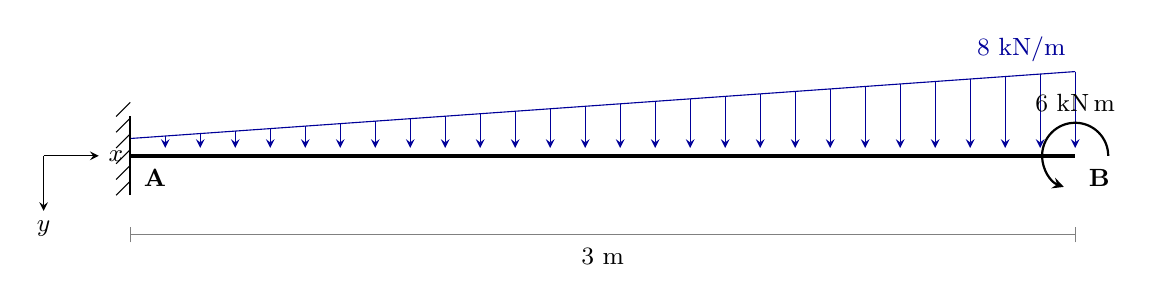
\begin{tikzpicture}
\draw[-stealth,blue!60!black] (0.4444,0.2515) -- (0.4444,0.1000);
\draw[-stealth,blue!60!black] (0.8889,0.2830) -- (0.8889,0.1000);
\draw[-stealth,blue!60!black] (1.3333,0.3144) -- (1.3333,0.1000);
\draw[-stealth,blue!60!black] (1.7778,0.3459) -- (1.7778,0.1000);
\draw[-stealth,blue!60!black] (2.2222,0.3774) -- (2.2222,0.1000);
\draw[-stealth,blue!60!black] (2.6667,0.4089) -- (2.6667,0.1000);
\draw[-stealth,blue!60!black] (3.1111,0.4404) -- (3.1111,0.1000);
\draw[-stealth,blue!60!black] (3.5556,0.4719) -- (3.5556,0.1000);
\draw[-stealth,blue!60!black] (4.0000,0.5033) -- (4.0000,0.1000);
\draw[-stealth,blue!60!black] (4.4444,0.5348) -- (4.4444,0.1000);
\draw[-stealth,blue!60!black] (4.8889,0.5663) -- (4.8889,0.1000);
\draw[-stealth,blue!60!black] (5.3333,0.5978) -- (5.3333,0.1000);
\draw[-stealth,blue!60!black] (5.7778,0.6293) -- (5.7778,0.1000);
\draw[-stealth,blue!60!black] (6.2222,0.6607) -- (6.2222,0.1000);
\draw[-stealth,blue!60!black] (6.6667,0.6922) -- (6.6667,0.1000);
\draw[-stealth,blue!60!black] (7.1111,0.7237) -- (7.1111,0.1000);
\draw[-stealth,blue!60!black] (7.5556,0.7552) -- (7.5556,0.1000);
\draw[-stealth,blue!60!black] (8.0000,0.7867) -- (8.0000,0.1000);
\draw[-stealth,blue!60!black] (8.4444,0.8181) -- (8.4444,0.1000);
\draw[-stealth,blue!60!black] (8.8889,0.8496) -- (8.8889,0.1000);
\draw[-stealth,blue!60!black] (9.3333,0.8811) -- (9.3333,0.1000);
\draw[-stealth,blue!60!black] (9.7778,0.9126) -- (9.7778,0.1000);
\draw[-stealth,blue!60!black] (10.2222,0.9441) -- (10.2222,0.1000);
\draw[-stealth,blue!60!black] (10.6667,0.9756) -- (10.6667,0.1000);
\draw[-stealth,blue!60!black] (11.1111,1.0070) -- (11.1111,0.1000);
\draw[-stealth,blue!60!black] (11.5556,1.0385) -- (11.5556,0.1000);
\draw[-stealth,blue!60!black] (12.0000,1.0700) -- (12.0000,0.1000);
% studium:at distributed 0 x=0 to=3 check=span
\draw[blue!60!black] (0.0000,0.2200) -- (0.4444,0.2515) -- (0.8889,0.2830) -- (1.3333,0.3144) -- (1.7778,0.3459) -- (2.2222,0.3774) -- (2.6667,0.4089) -- (3.1111,0.4404) -- (3.5556,0.4719) -- (4.0000,0.5033) -- (4.4444,0.5348) -- (4.8889,0.5663) -- (5.3333,0.5978) -- (5.7778,0.6293) -- (6.2222,0.6607) -- (6.6667,0.6922) -- (7.1111,0.7237) -- (7.5556,0.7552) -- (8.0000,0.7867) -- (8.4444,0.8181) -- (8.8889,0.8496) -- (9.3333,0.8811) -- (9.7778,0.9126) -- (10.2222,0.9441) -- (10.6667,0.9756) -- (11.1111,1.0070) -- (11.5556,1.0385) -- (12.0000,1.0700);
\node[font=\small,anchor=south east,blue!60!black] at (12.0000,1.0700) {$8$~\mbox{kN/m}};
\draw[line width=1.6pt] (0,0.0000) -- (12.0000,0.0000);
% studium:at support A x=0 check=first
\draw[thick] (0.0000,-0.5000) -- (0.0000,0.5000);
\draw (0.0000,-0.3200) -- (-0.1800,-0.5000);
\draw (0.0000,-0.1200) -- (-0.1800,-0.3000);
\draw (0.0000,0.0800) -- (-0.1800,-0.1000);
\draw (0.0000,0.2800) -- (-0.1800,0.1000);
\draw (0.0000,0.4800) -- (-0.1800,0.3000);
\draw (0.0000,0.6800) -- (-0.1800,0.5000);
% studium:at couple 0 x=3 check=first
\node[font=\small,anchor=south,black] at (12.0000,0.4400) {$6$~\mbox{kN\,m}};
\draw[-stealth,thick,black] (12.4200,0.0000) arc (0:250:0.42);
\node[font=\small\bfseries,anchor=north west] at (0.0500,-0.0500) {A};
\node[font=\small\bfseries,anchor=north west] at (12.0500,-0.0500) {B};
\draw[gray] (0,-1.0000) -- (12.0000,-1.0000);
\draw[gray] (0.0000,-1.1000) -- (0.0000,-0.9000);
\draw[gray] (12.0000,-1.1000) -- (12.0000,-0.9000);
\node[font=\small,anchor=north] at (6.0000,-1.0500) {$3$~\mbox{m}};
\draw[-stealth] (-1.1,0.0000) -- (-0.4,0.0000) node[right,font=\small] {$x$};
\draw[-stealth] (-1.1,0.0000) -- (-1.1,-0.7000) node[below,font=\small] {$y$};
\end{tikzpicture}}%
\count0=\ht0
\advance\count0 by \dp0
\count2=\wd0
\count4=\dimexpr\textheight/100*38\relax
\count6=\linewidth
\ifnum\count0<1
\count0=1
\fi
\ifnum\count2<1
\count2=1
\fi
\divide\count0 by 4096
\divide\count2 by 4096
\divide\count4 by 4096
\divide\count6 by 4096
\ifnum\count0<1
\count0=1
\fi
\ifnum\count2<1
\count2=1
\fi
\ifnum\count4<1
\count4=1
\fi
\ifnum\count6<1
\count6=1
\fi
\count8=\count2
\ifnum\count0>\count4
\count8=\numexpr\count2*\count4/\count0\relax
\fi
\ifnum\count8>\count6
\resizebox{\linewidth}{!}{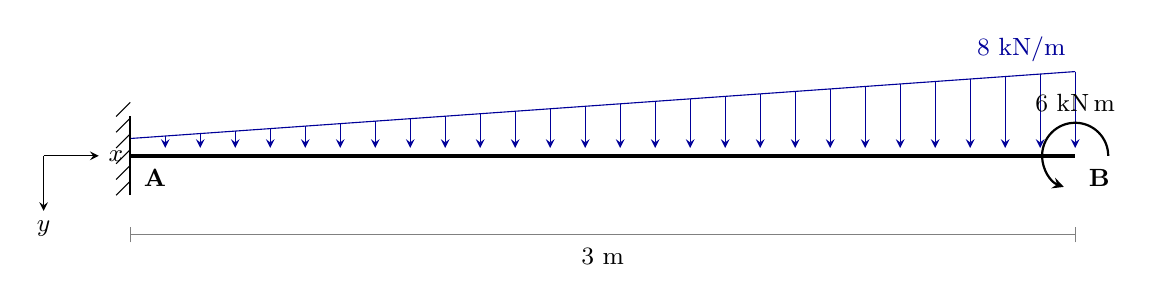
\begin{tikzpicture}
\draw[-stealth,blue!60!black] (0.4444,0.2515) -- (0.4444,0.1000);
\draw[-stealth,blue!60!black] (0.8889,0.2830) -- (0.8889,0.1000);
\draw[-stealth,blue!60!black] (1.3333,0.3144) -- (1.3333,0.1000);
\draw[-stealth,blue!60!black] (1.7778,0.3459) -- (1.7778,0.1000);
\draw[-stealth,blue!60!black] (2.2222,0.3774) -- (2.2222,0.1000);
\draw[-stealth,blue!60!black] (2.6667,0.4089) -- (2.6667,0.1000);
\draw[-stealth,blue!60!black] (3.1111,0.4404) -- (3.1111,0.1000);
\draw[-stealth,blue!60!black] (3.5556,0.4719) -- (3.5556,0.1000);
\draw[-stealth,blue!60!black] (4.0000,0.5033) -- (4.0000,0.1000);
\draw[-stealth,blue!60!black] (4.4444,0.5348) -- (4.4444,0.1000);
\draw[-stealth,blue!60!black] (4.8889,0.5663) -- (4.8889,0.1000);
\draw[-stealth,blue!60!black] (5.3333,0.5978) -- (5.3333,0.1000);
\draw[-stealth,blue!60!black] (5.7778,0.6293) -- (5.7778,0.1000);
\draw[-stealth,blue!60!black] (6.2222,0.6607) -- (6.2222,0.1000);
\draw[-stealth,blue!60!black] (6.6667,0.6922) -- (6.6667,0.1000);
\draw[-stealth,blue!60!black] (7.1111,0.7237) -- (7.1111,0.1000);
\draw[-stealth,blue!60!black] (7.5556,0.7552) -- (7.5556,0.1000);
\draw[-stealth,blue!60!black] (8.0000,0.7867) -- (8.0000,0.1000);
\draw[-stealth,blue!60!black] (8.4444,0.8181) -- (8.4444,0.1000);
\draw[-stealth,blue!60!black] (8.8889,0.8496) -- (8.8889,0.1000);
\draw[-stealth,blue!60!black] (9.3333,0.8811) -- (9.3333,0.1000);
\draw[-stealth,blue!60!black] (9.7778,0.9126) -- (9.7778,0.1000);
\draw[-stealth,blue!60!black] (10.2222,0.9441) -- (10.2222,0.1000);
\draw[-stealth,blue!60!black] (10.6667,0.9756) -- (10.6667,0.1000);
\draw[-stealth,blue!60!black] (11.1111,1.0070) -- (11.1111,0.1000);
\draw[-stealth,blue!60!black] (11.5556,1.0385) -- (11.5556,0.1000);
\draw[-stealth,blue!60!black] (12.0000,1.0700) -- (12.0000,0.1000);
% studium:at distributed 0 x=0 to=3 check=span
\draw[blue!60!black] (0.0000,0.2200) -- (0.4444,0.2515) -- (0.8889,0.2830) -- (1.3333,0.3144) -- (1.7778,0.3459) -- (2.2222,0.3774) -- (2.6667,0.4089) -- (3.1111,0.4404) -- (3.5556,0.4719) -- (4.0000,0.5033) -- (4.4444,0.5348) -- (4.8889,0.5663) -- (5.3333,0.5978) -- (5.7778,0.6293) -- (6.2222,0.6607) -- (6.6667,0.6922) -- (7.1111,0.7237) -- (7.5556,0.7552) -- (8.0000,0.7867) -- (8.4444,0.8181) -- (8.8889,0.8496) -- (9.3333,0.8811) -- (9.7778,0.9126) -- (10.2222,0.9441) -- (10.6667,0.9756) -- (11.1111,1.0070) -- (11.5556,1.0385) -- (12.0000,1.0700);
\node[font=\small,anchor=south east,blue!60!black] at (12.0000,1.0700) {$8$~\mbox{kN/m}};
\draw[line width=1.6pt] (0,0.0000) -- (12.0000,0.0000);
% studium:at support A x=0 check=first
\draw[thick] (0.0000,-0.5000) -- (0.0000,0.5000);
\draw (0.0000,-0.3200) -- (-0.1800,-0.5000);
\draw (0.0000,-0.1200) -- (-0.1800,-0.3000);
\draw (0.0000,0.0800) -- (-0.1800,-0.1000);
\draw (0.0000,0.2800) -- (-0.1800,0.1000);
\draw (0.0000,0.4800) -- (-0.1800,0.3000);
\draw (0.0000,0.6800) -- (-0.1800,0.5000);
% studium:at couple 0 x=3 check=first
\node[font=\small,anchor=south,black] at (12.0000,0.4400) {$6$~\mbox{kN\,m}};
\draw[-stealth,thick,black] (12.4200,0.0000) arc (0:250:0.42);
\node[font=\small\bfseries,anchor=north west] at (0.0500,-0.0500) {A};
\node[font=\small\bfseries,anchor=north west] at (12.0500,-0.0500) {B};
\draw[gray] (0,-1.0000) -- (12.0000,-1.0000);
\draw[gray] (0.0000,-1.1000) -- (0.0000,-0.9000);
\draw[gray] (12.0000,-1.1000) -- (12.0000,-0.9000);
\node[font=\small,anchor=north] at (6.0000,-1.0500) {$3$~\mbox{m}};
\draw[-stealth] (-1.1,0.0000) -- (-0.4,0.0000) node[right,font=\small] {$x$};
\draw[-stealth] (-1.1,0.0000) -- (-1.1,-0.7000) node[below,font=\small] {$y$};
\end{tikzpicture}}%
\else
\ifnum\count0>\count4
\resizebox{!}{\dimexpr\textheight/100*38\relax}{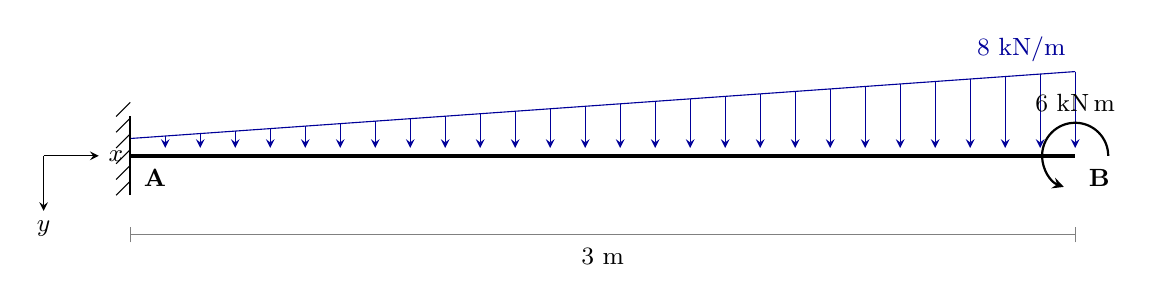
\begin{tikzpicture}
\draw[-stealth,blue!60!black] (0.4444,0.2515) -- (0.4444,0.1000);
\draw[-stealth,blue!60!black] (0.8889,0.2830) -- (0.8889,0.1000);
\draw[-stealth,blue!60!black] (1.3333,0.3144) -- (1.3333,0.1000);
\draw[-stealth,blue!60!black] (1.7778,0.3459) -- (1.7778,0.1000);
\draw[-stealth,blue!60!black] (2.2222,0.3774) -- (2.2222,0.1000);
\draw[-stealth,blue!60!black] (2.6667,0.4089) -- (2.6667,0.1000);
\draw[-stealth,blue!60!black] (3.1111,0.4404) -- (3.1111,0.1000);
\draw[-stealth,blue!60!black] (3.5556,0.4719) -- (3.5556,0.1000);
\draw[-stealth,blue!60!black] (4.0000,0.5033) -- (4.0000,0.1000);
\draw[-stealth,blue!60!black] (4.4444,0.5348) -- (4.4444,0.1000);
\draw[-stealth,blue!60!black] (4.8889,0.5663) -- (4.8889,0.1000);
\draw[-stealth,blue!60!black] (5.3333,0.5978) -- (5.3333,0.1000);
\draw[-stealth,blue!60!black] (5.7778,0.6293) -- (5.7778,0.1000);
\draw[-stealth,blue!60!black] (6.2222,0.6607) -- (6.2222,0.1000);
\draw[-stealth,blue!60!black] (6.6667,0.6922) -- (6.6667,0.1000);
\draw[-stealth,blue!60!black] (7.1111,0.7237) -- (7.1111,0.1000);
\draw[-stealth,blue!60!black] (7.5556,0.7552) -- (7.5556,0.1000);
\draw[-stealth,blue!60!black] (8.0000,0.7867) -- (8.0000,0.1000);
\draw[-stealth,blue!60!black] (8.4444,0.8181) -- (8.4444,0.1000);
\draw[-stealth,blue!60!black] (8.8889,0.8496) -- (8.8889,0.1000);
\draw[-stealth,blue!60!black] (9.3333,0.8811) -- (9.3333,0.1000);
\draw[-stealth,blue!60!black] (9.7778,0.9126) -- (9.7778,0.1000);
\draw[-stealth,blue!60!black] (10.2222,0.9441) -- (10.2222,0.1000);
\draw[-stealth,blue!60!black] (10.6667,0.9756) -- (10.6667,0.1000);
\draw[-stealth,blue!60!black] (11.1111,1.0070) -- (11.1111,0.1000);
\draw[-stealth,blue!60!black] (11.5556,1.0385) -- (11.5556,0.1000);
\draw[-stealth,blue!60!black] (12.0000,1.0700) -- (12.0000,0.1000);
% studium:at distributed 0 x=0 to=3 check=span
\draw[blue!60!black] (0.0000,0.2200) -- (0.4444,0.2515) -- (0.8889,0.2830) -- (1.3333,0.3144) -- (1.7778,0.3459) -- (2.2222,0.3774) -- (2.6667,0.4089) -- (3.1111,0.4404) -- (3.5556,0.4719) -- (4.0000,0.5033) -- (4.4444,0.5348) -- (4.8889,0.5663) -- (5.3333,0.5978) -- (5.7778,0.6293) -- (6.2222,0.6607) -- (6.6667,0.6922) -- (7.1111,0.7237) -- (7.5556,0.7552) -- (8.0000,0.7867) -- (8.4444,0.8181) -- (8.8889,0.8496) -- (9.3333,0.8811) -- (9.7778,0.9126) -- (10.2222,0.9441) -- (10.6667,0.9756) -- (11.1111,1.0070) -- (11.5556,1.0385) -- (12.0000,1.0700);
\node[font=\small,anchor=south east,blue!60!black] at (12.0000,1.0700) {$8$~\mbox{kN/m}};
\draw[line width=1.6pt] (0,0.0000) -- (12.0000,0.0000);
% studium:at support A x=0 check=first
\draw[thick] (0.0000,-0.5000) -- (0.0000,0.5000);
\draw (0.0000,-0.3200) -- (-0.1800,-0.5000);
\draw (0.0000,-0.1200) -- (-0.1800,-0.3000);
\draw (0.0000,0.0800) -- (-0.1800,-0.1000);
\draw (0.0000,0.2800) -- (-0.1800,0.1000);
\draw (0.0000,0.4800) -- (-0.1800,0.3000);
\draw (0.0000,0.6800) -- (-0.1800,0.5000);
% studium:at couple 0 x=3 check=first
\node[font=\small,anchor=south,black] at (12.0000,0.4400) {$6$~\mbox{kN\,m}};
\draw[-stealth,thick,black] (12.4200,0.0000) arc (0:250:0.42);
\node[font=\small\bfseries,anchor=north west] at (0.0500,-0.0500) {A};
\node[font=\small\bfseries,anchor=north west] at (12.0500,-0.0500) {B};
\draw[gray] (0,-1.0000) -- (12.0000,-1.0000);
\draw[gray] (0.0000,-1.1000) -- (0.0000,-0.9000);
\draw[gray] (12.0000,-1.1000) -- (12.0000,-0.9000);
\node[font=\small,anchor=north] at (6.0000,-1.0500) {$3$~\mbox{m}};
\draw[-stealth] (-1.1,0.0000) -- (-0.4,0.0000) node[right,font=\small] {$x$};
\draw[-stealth] (-1.1,0.0000) -- (-1.1,-0.7000) node[below,font=\small] {$y$};
\end{tikzpicture}}%
\else
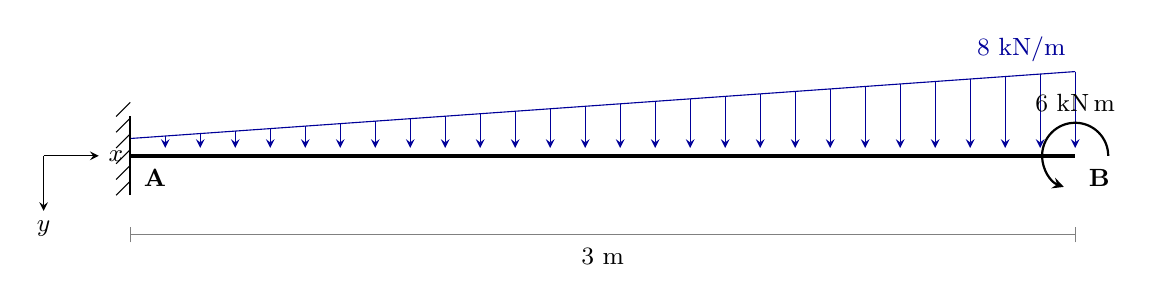
\begin{tikzpicture}
\draw[-stealth,blue!60!black] (0.4444,0.2515) -- (0.4444,0.1000);
\draw[-stealth,blue!60!black] (0.8889,0.2830) -- (0.8889,0.1000);
\draw[-stealth,blue!60!black] (1.3333,0.3144) -- (1.3333,0.1000);
\draw[-stealth,blue!60!black] (1.7778,0.3459) -- (1.7778,0.1000);
\draw[-stealth,blue!60!black] (2.2222,0.3774) -- (2.2222,0.1000);
\draw[-stealth,blue!60!black] (2.6667,0.4089) -- (2.6667,0.1000);
\draw[-stealth,blue!60!black] (3.1111,0.4404) -- (3.1111,0.1000);
\draw[-stealth,blue!60!black] (3.5556,0.4719) -- (3.5556,0.1000);
\draw[-stealth,blue!60!black] (4.0000,0.5033) -- (4.0000,0.1000);
\draw[-stealth,blue!60!black] (4.4444,0.5348) -- (4.4444,0.1000);
\draw[-stealth,blue!60!black] (4.8889,0.5663) -- (4.8889,0.1000);
\draw[-stealth,blue!60!black] (5.3333,0.5978) -- (5.3333,0.1000);
\draw[-stealth,blue!60!black] (5.7778,0.6293) -- (5.7778,0.1000);
\draw[-stealth,blue!60!black] (6.2222,0.6607) -- (6.2222,0.1000);
\draw[-stealth,blue!60!black] (6.6667,0.6922) -- (6.6667,0.1000);
\draw[-stealth,blue!60!black] (7.1111,0.7237) -- (7.1111,0.1000);
\draw[-stealth,blue!60!black] (7.5556,0.7552) -- (7.5556,0.1000);
\draw[-stealth,blue!60!black] (8.0000,0.7867) -- (8.0000,0.1000);
\draw[-stealth,blue!60!black] (8.4444,0.8181) -- (8.4444,0.1000);
\draw[-stealth,blue!60!black] (8.8889,0.8496) -- (8.8889,0.1000);
\draw[-stealth,blue!60!black] (9.3333,0.8811) -- (9.3333,0.1000);
\draw[-stealth,blue!60!black] (9.7778,0.9126) -- (9.7778,0.1000);
\draw[-stealth,blue!60!black] (10.2222,0.9441) -- (10.2222,0.1000);
\draw[-stealth,blue!60!black] (10.6667,0.9756) -- (10.6667,0.1000);
\draw[-stealth,blue!60!black] (11.1111,1.0070) -- (11.1111,0.1000);
\draw[-stealth,blue!60!black] (11.5556,1.0385) -- (11.5556,0.1000);
\draw[-stealth,blue!60!black] (12.0000,1.0700) -- (12.0000,0.1000);
% studium:at distributed 0 x=0 to=3 check=span
\draw[blue!60!black] (0.0000,0.2200) -- (0.4444,0.2515) -- (0.8889,0.2830) -- (1.3333,0.3144) -- (1.7778,0.3459) -- (2.2222,0.3774) -- (2.6667,0.4089) -- (3.1111,0.4404) -- (3.5556,0.4719) -- (4.0000,0.5033) -- (4.4444,0.5348) -- (4.8889,0.5663) -- (5.3333,0.5978) -- (5.7778,0.6293) -- (6.2222,0.6607) -- (6.6667,0.6922) -- (7.1111,0.7237) -- (7.5556,0.7552) -- (8.0000,0.7867) -- (8.4444,0.8181) -- (8.8889,0.8496) -- (9.3333,0.8811) -- (9.7778,0.9126) -- (10.2222,0.9441) -- (10.6667,0.9756) -- (11.1111,1.0070) -- (11.5556,1.0385) -- (12.0000,1.0700);
\node[font=\small,anchor=south east,blue!60!black] at (12.0000,1.0700) {$8$~\mbox{kN/m}};
\draw[line width=1.6pt] (0,0.0000) -- (12.0000,0.0000);
% studium:at support A x=0 check=first
\draw[thick] (0.0000,-0.5000) -- (0.0000,0.5000);
\draw (0.0000,-0.3200) -- (-0.1800,-0.5000);
\draw (0.0000,-0.1200) -- (-0.1800,-0.3000);
\draw (0.0000,0.0800) -- (-0.1800,-0.1000);
\draw (0.0000,0.2800) -- (-0.1800,0.1000);
\draw (0.0000,0.4800) -- (-0.1800,0.3000);
\draw (0.0000,0.6800) -- (-0.1800,0.5000);
% studium:at couple 0 x=3 check=first
\node[font=\small,anchor=south,black] at (12.0000,0.4400) {$6$~\mbox{kN\,m}};
\draw[-stealth,thick,black] (12.4200,0.0000) arc (0:250:0.42);
\node[font=\small\bfseries,anchor=north west] at (0.0500,-0.0500) {A};
\node[font=\small\bfseries,anchor=north west] at (12.0500,-0.0500) {B};
\draw[gray] (0,-1.0000) -- (12.0000,-1.0000);
\draw[gray] (0.0000,-1.1000) -- (0.0000,-0.9000);
\draw[gray] (12.0000,-1.1000) -- (12.0000,-0.9000);
\node[font=\small,anchor=north] at (6.0000,-1.0500) {$3$~\mbox{m}};
\draw[-stealth] (-1.1,0.0000) -- (-0.4,0.0000) node[right,font=\small] {$x$};
\draw[-stealth] (-1.1,0.0000) -- (-1.1,-0.7000) node[below,font=\small] {$y$};
\end{tikzpicture}%
\fi
\fi
\endgroup
\par\nopagebreak
\studiumcaption{fig:e2-c03-mens-enunciado}{Ménsula con carga triangular y momento en el extremo libre.}
\end{minipage}\par\medskip

\textbf{Hipótesis.}\begin{itemize}\item ménsula isostática empotrada en $x = 0$
\item cortante positivo si levanta la cara izquierda y flector positivo si comprime arriba\end{itemize}

\textbf{Modelo y desarrollo.}

Resultante de la carga triangular.\[\fitmath{Q = \frac{q_0\,L}{2}}\]

\textbf{Procedimiento.}\begin{itemize}\item La carga vale $q(x) = q_0\,x/L$ y su resultante, $Q = q_0 L/2$, actúa a $\tfrac{2}{3}L$ del empotramiento.
\item Las fuerzas verticales dan la reacción $R_A = Q$, hacia arriba.
\item Con la parte derecha de la sección, la carga entre $x$ y $L$ y el momento $M_0$ dan $C_y(x) = q_0 (L^2 - x^2)/(2L)$ y $M_z(x) = -q_0 (L - x)^2 (2L + x)/(6L) + M_0$.
\item En el empotramiento el flector es $M_z(0) = -q_0 L^2/3 + M_0$; en el extremo libre vale $M_0$.\end{itemize}

\textbf{Cálculo de los pasos.}

\begin{enumerate}

\item Resultante de la carga.

\[\fitmath{y_{1}=\frac{8\cdot 3}{2}\approx 12\,\mathrm{kN}}\]

\item Reacción vertical en A.

\[\fitmath{y_{2}=\frac{8\cdot 3}{2}\approx 12\,\mathrm{kN}}\]

\item Flector en el extremo libre.

\[\fitmath{y_{3}=6\approx 6\,\mathrm{kN m}}\]

\item Flector en el empotramiento.

\[\fitmath{y_{4}=\frac{-8\cdot {3}^{2}}{3}+6\approx -18\,\mathrm{kN m}}\]

\end{enumerate}

\par\medskip\noindent\begin{minipage}{\linewidth}
\centering
\begingroup
\setbox0=\hbox{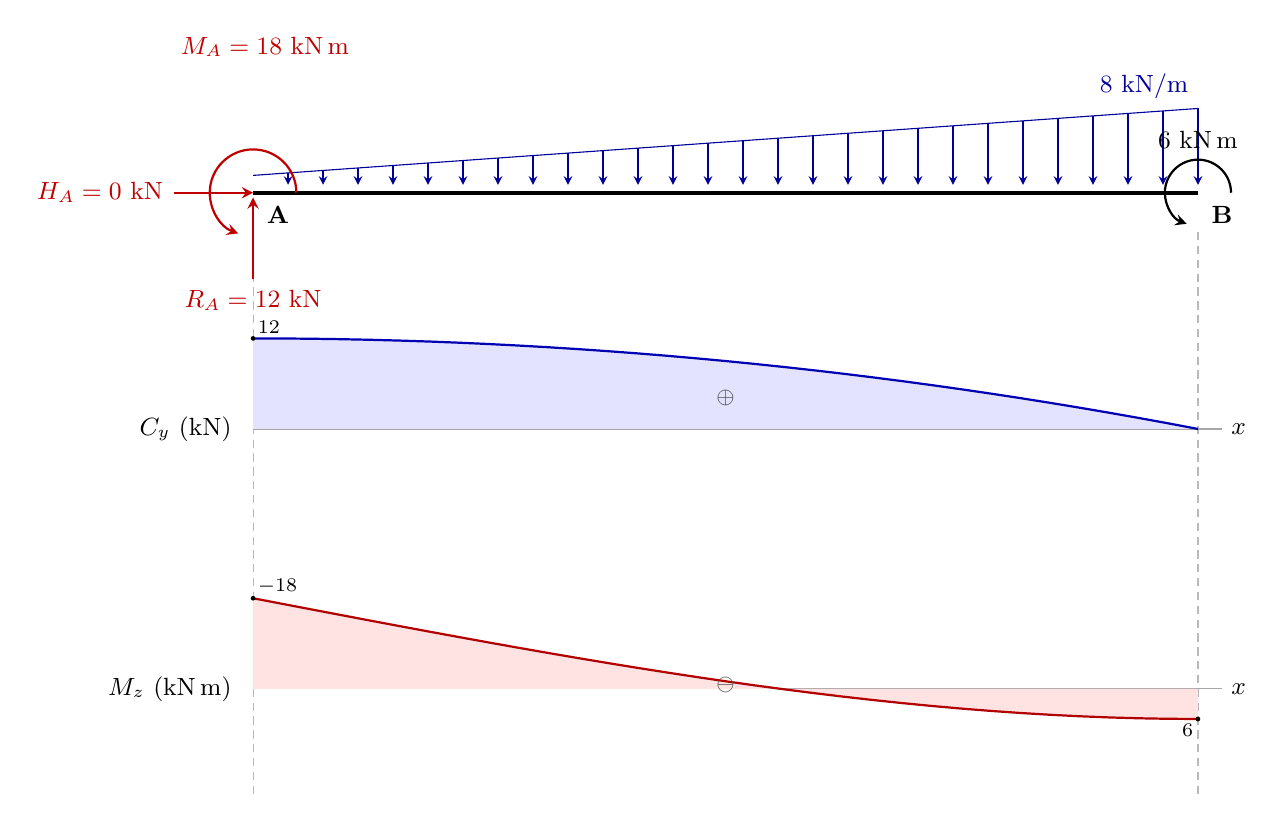
\begin{tikzpicture}
\draw[densely dashed,gray!55] (12.0000,-0.5000) -- (12.0000,-7.7000);
\draw[densely dashed,gray!55] (0.0000,-0.5000) -- (0.0000,-7.7000);
\draw[-stealth,blue!60!black] (0.4444,0.2515) -- (0.4444,0.1000);
\draw[-stealth,blue!60!black] (0.8889,0.2830) -- (0.8889,0.1000);
\draw[-stealth,blue!60!black] (1.3333,0.3144) -- (1.3333,0.1000);
\draw[-stealth,blue!60!black] (1.7778,0.3459) -- (1.7778,0.1000);
\draw[-stealth,blue!60!black] (2.2222,0.3774) -- (2.2222,0.1000);
\draw[-stealth,blue!60!black] (2.6667,0.4089) -- (2.6667,0.1000);
\draw[-stealth,blue!60!black] (3.1111,0.4404) -- (3.1111,0.1000);
\draw[-stealth,blue!60!black] (3.5556,0.4719) -- (3.5556,0.1000);
\draw[-stealth,blue!60!black] (4.0000,0.5033) -- (4.0000,0.1000);
\draw[-stealth,blue!60!black] (4.4444,0.5348) -- (4.4444,0.1000);
\draw[-stealth,blue!60!black] (4.8889,0.5663) -- (4.8889,0.1000);
\draw[-stealth,blue!60!black] (5.3333,0.5978) -- (5.3333,0.1000);
\draw[-stealth,blue!60!black] (5.7778,0.6293) -- (5.7778,0.1000);
\draw[-stealth,blue!60!black] (6.2222,0.6607) -- (6.2222,0.1000);
\draw[-stealth,blue!60!black] (6.6667,0.6922) -- (6.6667,0.1000);
\draw[-stealth,blue!60!black] (7.1111,0.7237) -- (7.1111,0.1000);
\draw[-stealth,blue!60!black] (7.5556,0.7552) -- (7.5556,0.1000);
\draw[-stealth,blue!60!black] (8.0000,0.7867) -- (8.0000,0.1000);
\draw[-stealth,blue!60!black] (8.4444,0.8181) -- (8.4444,0.1000);
\draw[-stealth,blue!60!black] (8.8889,0.8496) -- (8.8889,0.1000);
\draw[-stealth,blue!60!black] (9.3333,0.8811) -- (9.3333,0.1000);
\draw[-stealth,blue!60!black] (9.7778,0.9126) -- (9.7778,0.1000);
\draw[-stealth,blue!60!black] (10.2222,0.9441) -- (10.2222,0.1000);
\draw[-stealth,blue!60!black] (10.6667,0.9756) -- (10.6667,0.1000);
\draw[-stealth,blue!60!black] (11.1111,1.0070) -- (11.1111,0.1000);
\draw[-stealth,blue!60!black] (11.5556,1.0385) -- (11.5556,0.1000);
\draw[-stealth,blue!60!black] (12.0000,1.0700) -- (12.0000,0.1000);
% studium:at distributed 0 x=0 to=3 check=span
\draw[blue!60!black] (0.0000,0.2200) -- (0.4444,0.2515) -- (0.8889,0.2830) -- (1.3333,0.3144) -- (1.7778,0.3459) -- (2.2222,0.3774) -- (2.6667,0.4089) -- (3.1111,0.4404) -- (3.5556,0.4719) -- (4.0000,0.5033) -- (4.4444,0.5348) -- (4.8889,0.5663) -- (5.3333,0.5978) -- (5.7778,0.6293) -- (6.2222,0.6607) -- (6.6667,0.6922) -- (7.1111,0.7237) -- (7.5556,0.7552) -- (8.0000,0.7867) -- (8.4444,0.8181) -- (8.8889,0.8496) -- (9.3333,0.8811) -- (9.7778,0.9126) -- (10.2222,0.9441) -- (10.6667,0.9756) -- (11.1111,1.0070) -- (11.5556,1.0385) -- (12.0000,1.0700);
\node[font=\small,anchor=south east,blue!60!black] at (12.0000,1.0700) {$8$~\mbox{kN/m}};
\draw[line width=1.6pt] (0,0.0000) -- (12.0000,0.0000);
% studium:at couple 0 x=3 check=first
\node[font=\small,anchor=south,black] at (12.0000,0.4400) {$6$~\mbox{kN\,m}};
\draw[-stealth,thick,black] (12.4200,0.0000) arc (0:250:0.42);
% studium:reaction H_A value=0
% studium:at reaction H_A x=0 check=tip
\draw[-stealth,thick,red!75!black] (-1.0000,0.0000) -- (0.0000,0.0000);
\node[font=\small,anchor=east,red!75!black] at (-1.0200,0.0000) {$H_{A} = 0$~\mbox{kN}};
% studium:reaction R_A value=12
% studium:at reaction R_A x=0 check=tip
\draw[-stealth,thick,red!75!black] (0.0000,-1.1000) -- (0.0000,-0.0600);
\node[font=\small,anchor=north,red!75!black] at (0.0000,-1.1200) {$R_{A} = 12$~\mbox{kN}};
% studium:reaction M_A value=18
% studium:at reaction M_A x=0 check=arc
\draw[-stealth,thick,red!75!black] (0.5500,0.0000) arc (0:250:0.55);
\node[font=\small,anchor=south,red!75!black] at (0.1500,1.6000) {$M_{A} = 18$~\mbox{kN\,m}};
\node[font=\small\bfseries,anchor=north west] at (0.0500,-0.0500) {A};
\node[font=\small\bfseries,anchor=north west] at (12.0500,-0.0500) {B};
\draw[gray!70] (0,-3.0000) -- (12.3000,-3.0000);
\fill[blue!11] (0.0000,-3.0000) -- (0.0000,-1.8500) -- (0.3750,-1.8511) -- (0.7500,-1.8545) -- (1.1250,-1.8601) -- (1.5000,-1.8680) -- (1.8750,-1.8781) -- (2.2500,-1.8904) -- (2.6250,-1.9050) -- (3.0000,-1.9219) -- (3.3750,-1.9410) -- (3.7500,-1.9623) -- (4.1250,-1.9859) -- (4.5000,-2.0117) -- (4.8750,-2.0398) -- (5.2500,-2.0701) -- (5.6250,-2.1027) -- (6.0000,-2.1375) -- (6.3750,-2.1746) -- (6.7500,-2.2139) -- (7.1250,-2.2554) -- (7.5000,-2.2992) -- (7.8750,-2.3453) -- (8.2500,-2.3936) -- (8.6250,-2.4441) -- (9.0000,-2.4969) -- (9.3750,-2.5519) -- (9.7500,-2.6092) -- (10.1250,-2.6687) -- (10.5000,-2.7305) -- (10.8750,-2.7945) -- (11.2500,-2.8607) -- (11.6250,-2.9292) -- (12.0000,-3.0000) -- (12.0000,-3.0000) -- cycle;
% studium:series V sx=4.0 sy=0.09583333333333333 x0=0.0 y0=-3.0 sign=1
\draw[thick,blue!70!black] (0.0000,-1.8500) -- (0.3750,-1.8511) -- (0.7500,-1.8545) -- (1.1250,-1.8601) -- (1.5000,-1.8680) -- (1.8750,-1.8781) -- (2.2500,-1.8904) -- (2.6250,-1.9050) -- (3.0000,-1.9219) -- (3.3750,-1.9410) -- (3.7500,-1.9623) -- (4.1250,-1.9859) -- (4.5000,-2.0117) -- (4.8750,-2.0398) -- (5.2500,-2.0701) -- (5.6250,-2.1027) -- (6.0000,-2.1375) -- (6.3750,-2.1746) -- (6.7500,-2.2139) -- (7.1250,-2.2554) -- (7.5000,-2.2992) -- (7.8750,-2.3453) -- (8.2500,-2.3936) -- (8.6250,-2.4441) -- (9.0000,-2.4969) -- (9.3750,-2.5519) -- (9.7500,-2.6092) -- (10.1250,-2.6687) -- (10.5000,-2.7305) -- (10.8750,-2.7945) -- (11.2500,-2.8607) -- (11.6250,-2.9292) -- (12.0000,-3.0000);
% studium:end V
\node[font=\small,anchor=east] at (-0.15,-3.0000) {$C_y$ (kN)};
\node[font=\small,anchor=west] at (12.3000,-3.0000) {$x$};
% studium:label V x=0 side=right value=12
\fill (0.0000,-1.8500) circle (0.03);
\node[font=\scriptsize,anchor=south west,inner sep=1.5pt] at (0.0000,-1.8500) {$12$};
\node[font=\footnotesize,gray!60!black] at (6.0000,-2.6119) {$\oplus$};
\draw[gray!70] (0,-6.3000) -- (12.3000,-6.3000);
\fill[red!11] (0.0000,-6.3000) -- (0.0000,-5.1500) -- (0.3750,-5.2219) -- (0.7500,-5.2936) -- (1.1250,-5.3650) -- (1.5000,-5.4360) -- (1.8750,-5.5065) -- (2.2500,-5.5762) -- (2.6250,-5.6451) -- (3.0000,-5.7130) -- (3.3750,-5.7798) -- (3.7500,-5.8454) -- (4.1250,-5.9095) -- (4.5000,-5.9721) -- (4.8750,-6.0330) -- (5.2500,-6.0920) -- (5.6250,-6.1492) -- (6.0000,-6.2042) -- (6.3750,-6.2569) -- (6.7500,-6.3073) -- (7.1250,-6.3551) -- (7.5000,-6.4003) -- (7.8750,-6.4427) -- (8.2500,-6.4821) -- (8.6250,-6.5185) -- (9.0000,-6.5516) -- (9.3750,-6.5813) -- (9.7500,-6.6075) -- (10.1250,-6.6301) -- (10.5000,-6.6489) -- (10.8750,-6.6638) -- (11.2500,-6.6745) -- (11.6250,-6.6811) -- (12.0000,-6.6833) -- (12.0000,-6.3000) -- cycle;
% studium:series M sx=4.0 sy=0.06388888888888888 x0=0.0 y0=-6.3 sign=-1
\draw[thick,red!70!black] (0.0000,-5.1500) -- (0.3750,-5.2219) -- (0.7500,-5.2936) -- (1.1250,-5.3650) -- (1.5000,-5.4360) -- (1.8750,-5.5065) -- (2.2500,-5.5762) -- (2.6250,-5.6451) -- (3.0000,-5.7130) -- (3.3750,-5.7798) -- (3.7500,-5.8454) -- (4.1250,-5.9095) -- (4.5000,-5.9721) -- (4.8750,-6.0330) -- (5.2500,-6.0920) -- (5.6250,-6.1492) -- (6.0000,-6.2042) -- (6.3750,-6.2569) -- (6.7500,-6.3073) -- (7.1250,-6.3551) -- (7.5000,-6.4003) -- (7.8750,-6.4427) -- (8.2500,-6.4821) -- (8.6250,-6.5185) -- (9.0000,-6.5516) -- (9.3750,-6.5813) -- (9.7500,-6.6075) -- (10.1250,-6.6301) -- (10.5000,-6.6489) -- (10.8750,-6.6638) -- (11.2500,-6.6745) -- (11.6250,-6.6811) -- (12.0000,-6.6833);
% studium:end M
\node[font=\small,anchor=east] at (-0.15,-6.3000) {$M_z$ (kN\,m)};
\node[font=\small,anchor=west] at (12.3000,-6.3000) {$x$};
% studium:label M x=0 side=right value=-18
\fill (0.0000,-5.1500) circle (0.03);
\node[font=\scriptsize,anchor=south west,inner sep=1.5pt] at (0.0000,-5.1500) {$-18$};
% studium:label M x=3 side=left value=6
\fill (12.0000,-6.6833) circle (0.03);
\node[font=\scriptsize,anchor=north east,inner sep=1.5pt] at (12.0000,-6.6833) {$6$};
\node[font=\footnotesize,gray!60!black] at (6.0000,-6.2569) {$\ominus$};
\end{tikzpicture}}%
\count0=\ht0
\advance\count0 by \dp0
\count2=\wd0
\count4=\dimexpr\textheight/100*38\relax
\count6=\linewidth
\ifnum\count0<1
\count0=1
\fi
\ifnum\count2<1
\count2=1
\fi
\divide\count0 by 4096
\divide\count2 by 4096
\divide\count4 by 4096
\divide\count6 by 4096
\ifnum\count0<1
\count0=1
\fi
\ifnum\count2<1
\count2=1
\fi
\ifnum\count4<1
\count4=1
\fi
\ifnum\count6<1
\count6=1
\fi
\count8=\count2
\ifnum\count0>\count4
\count8=\numexpr\count2*\count4/\count0\relax
\fi
\ifnum\count8>\count6
\resizebox{\linewidth}{!}{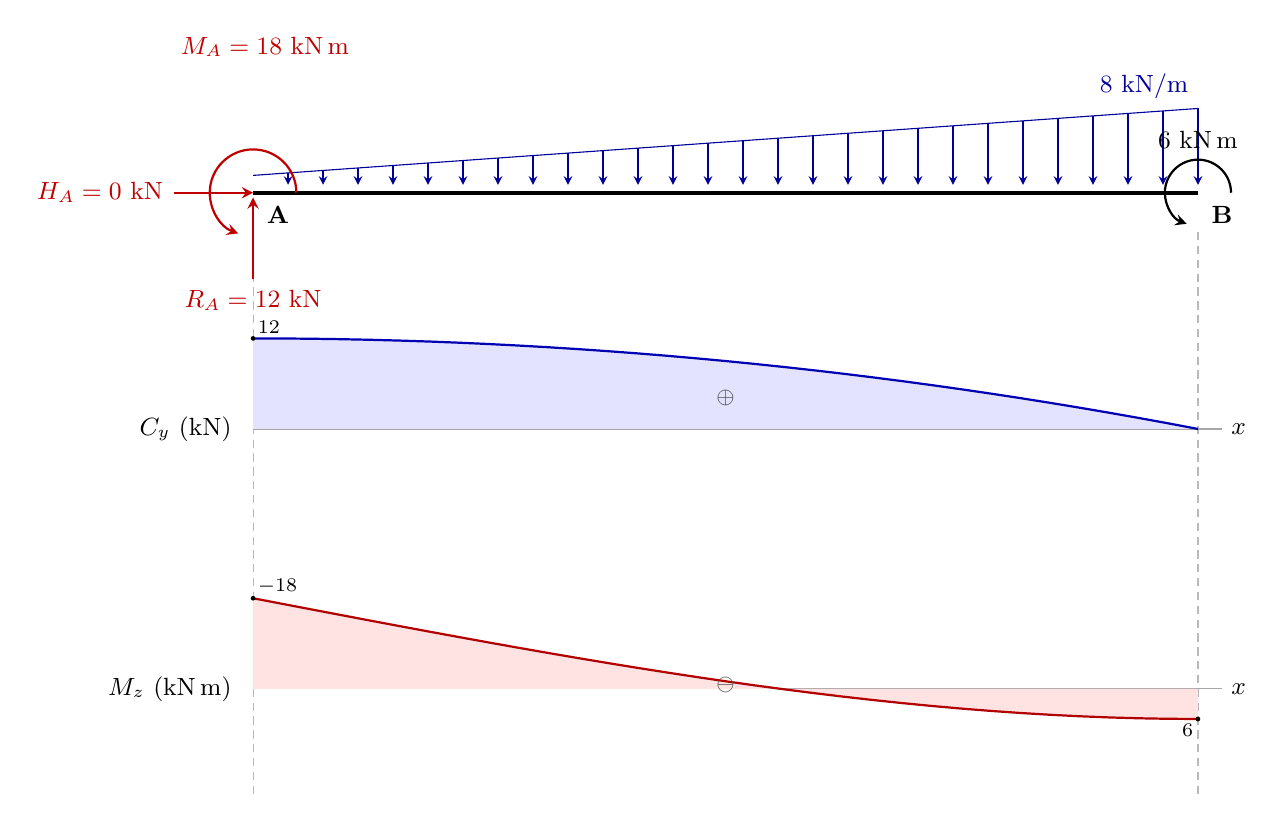
\begin{tikzpicture}
\draw[densely dashed,gray!55] (12.0000,-0.5000) -- (12.0000,-7.7000);
\draw[densely dashed,gray!55] (0.0000,-0.5000) -- (0.0000,-7.7000);
\draw[-stealth,blue!60!black] (0.4444,0.2515) -- (0.4444,0.1000);
\draw[-stealth,blue!60!black] (0.8889,0.2830) -- (0.8889,0.1000);
\draw[-stealth,blue!60!black] (1.3333,0.3144) -- (1.3333,0.1000);
\draw[-stealth,blue!60!black] (1.7778,0.3459) -- (1.7778,0.1000);
\draw[-stealth,blue!60!black] (2.2222,0.3774) -- (2.2222,0.1000);
\draw[-stealth,blue!60!black] (2.6667,0.4089) -- (2.6667,0.1000);
\draw[-stealth,blue!60!black] (3.1111,0.4404) -- (3.1111,0.1000);
\draw[-stealth,blue!60!black] (3.5556,0.4719) -- (3.5556,0.1000);
\draw[-stealth,blue!60!black] (4.0000,0.5033) -- (4.0000,0.1000);
\draw[-stealth,blue!60!black] (4.4444,0.5348) -- (4.4444,0.1000);
\draw[-stealth,blue!60!black] (4.8889,0.5663) -- (4.8889,0.1000);
\draw[-stealth,blue!60!black] (5.3333,0.5978) -- (5.3333,0.1000);
\draw[-stealth,blue!60!black] (5.7778,0.6293) -- (5.7778,0.1000);
\draw[-stealth,blue!60!black] (6.2222,0.6607) -- (6.2222,0.1000);
\draw[-stealth,blue!60!black] (6.6667,0.6922) -- (6.6667,0.1000);
\draw[-stealth,blue!60!black] (7.1111,0.7237) -- (7.1111,0.1000);
\draw[-stealth,blue!60!black] (7.5556,0.7552) -- (7.5556,0.1000);
\draw[-stealth,blue!60!black] (8.0000,0.7867) -- (8.0000,0.1000);
\draw[-stealth,blue!60!black] (8.4444,0.8181) -- (8.4444,0.1000);
\draw[-stealth,blue!60!black] (8.8889,0.8496) -- (8.8889,0.1000);
\draw[-stealth,blue!60!black] (9.3333,0.8811) -- (9.3333,0.1000);
\draw[-stealth,blue!60!black] (9.7778,0.9126) -- (9.7778,0.1000);
\draw[-stealth,blue!60!black] (10.2222,0.9441) -- (10.2222,0.1000);
\draw[-stealth,blue!60!black] (10.6667,0.9756) -- (10.6667,0.1000);
\draw[-stealth,blue!60!black] (11.1111,1.0070) -- (11.1111,0.1000);
\draw[-stealth,blue!60!black] (11.5556,1.0385) -- (11.5556,0.1000);
\draw[-stealth,blue!60!black] (12.0000,1.0700) -- (12.0000,0.1000);
% studium:at distributed 0 x=0 to=3 check=span
\draw[blue!60!black] (0.0000,0.2200) -- (0.4444,0.2515) -- (0.8889,0.2830) -- (1.3333,0.3144) -- (1.7778,0.3459) -- (2.2222,0.3774) -- (2.6667,0.4089) -- (3.1111,0.4404) -- (3.5556,0.4719) -- (4.0000,0.5033) -- (4.4444,0.5348) -- (4.8889,0.5663) -- (5.3333,0.5978) -- (5.7778,0.6293) -- (6.2222,0.6607) -- (6.6667,0.6922) -- (7.1111,0.7237) -- (7.5556,0.7552) -- (8.0000,0.7867) -- (8.4444,0.8181) -- (8.8889,0.8496) -- (9.3333,0.8811) -- (9.7778,0.9126) -- (10.2222,0.9441) -- (10.6667,0.9756) -- (11.1111,1.0070) -- (11.5556,1.0385) -- (12.0000,1.0700);
\node[font=\small,anchor=south east,blue!60!black] at (12.0000,1.0700) {$8$~\mbox{kN/m}};
\draw[line width=1.6pt] (0,0.0000) -- (12.0000,0.0000);
% studium:at couple 0 x=3 check=first
\node[font=\small,anchor=south,black] at (12.0000,0.4400) {$6$~\mbox{kN\,m}};
\draw[-stealth,thick,black] (12.4200,0.0000) arc (0:250:0.42);
% studium:reaction H_A value=0
% studium:at reaction H_A x=0 check=tip
\draw[-stealth,thick,red!75!black] (-1.0000,0.0000) -- (0.0000,0.0000);
\node[font=\small,anchor=east,red!75!black] at (-1.0200,0.0000) {$H_{A} = 0$~\mbox{kN}};
% studium:reaction R_A value=12
% studium:at reaction R_A x=0 check=tip
\draw[-stealth,thick,red!75!black] (0.0000,-1.1000) -- (0.0000,-0.0600);
\node[font=\small,anchor=north,red!75!black] at (0.0000,-1.1200) {$R_{A} = 12$~\mbox{kN}};
% studium:reaction M_A value=18
% studium:at reaction M_A x=0 check=arc
\draw[-stealth,thick,red!75!black] (0.5500,0.0000) arc (0:250:0.55);
\node[font=\small,anchor=south,red!75!black] at (0.1500,1.6000) {$M_{A} = 18$~\mbox{kN\,m}};
\node[font=\small\bfseries,anchor=north west] at (0.0500,-0.0500) {A};
\node[font=\small\bfseries,anchor=north west] at (12.0500,-0.0500) {B};
\draw[gray!70] (0,-3.0000) -- (12.3000,-3.0000);
\fill[blue!11] (0.0000,-3.0000) -- (0.0000,-1.8500) -- (0.3750,-1.8511) -- (0.7500,-1.8545) -- (1.1250,-1.8601) -- (1.5000,-1.8680) -- (1.8750,-1.8781) -- (2.2500,-1.8904) -- (2.6250,-1.9050) -- (3.0000,-1.9219) -- (3.3750,-1.9410) -- (3.7500,-1.9623) -- (4.1250,-1.9859) -- (4.5000,-2.0117) -- (4.8750,-2.0398) -- (5.2500,-2.0701) -- (5.6250,-2.1027) -- (6.0000,-2.1375) -- (6.3750,-2.1746) -- (6.7500,-2.2139) -- (7.1250,-2.2554) -- (7.5000,-2.2992) -- (7.8750,-2.3453) -- (8.2500,-2.3936) -- (8.6250,-2.4441) -- (9.0000,-2.4969) -- (9.3750,-2.5519) -- (9.7500,-2.6092) -- (10.1250,-2.6687) -- (10.5000,-2.7305) -- (10.8750,-2.7945) -- (11.2500,-2.8607) -- (11.6250,-2.9292) -- (12.0000,-3.0000) -- (12.0000,-3.0000) -- cycle;
% studium:series V sx=4.0 sy=0.09583333333333333 x0=0.0 y0=-3.0 sign=1
\draw[thick,blue!70!black] (0.0000,-1.8500) -- (0.3750,-1.8511) -- (0.7500,-1.8545) -- (1.1250,-1.8601) -- (1.5000,-1.8680) -- (1.8750,-1.8781) -- (2.2500,-1.8904) -- (2.6250,-1.9050) -- (3.0000,-1.9219) -- (3.3750,-1.9410) -- (3.7500,-1.9623) -- (4.1250,-1.9859) -- (4.5000,-2.0117) -- (4.8750,-2.0398) -- (5.2500,-2.0701) -- (5.6250,-2.1027) -- (6.0000,-2.1375) -- (6.3750,-2.1746) -- (6.7500,-2.2139) -- (7.1250,-2.2554) -- (7.5000,-2.2992) -- (7.8750,-2.3453) -- (8.2500,-2.3936) -- (8.6250,-2.4441) -- (9.0000,-2.4969) -- (9.3750,-2.5519) -- (9.7500,-2.6092) -- (10.1250,-2.6687) -- (10.5000,-2.7305) -- (10.8750,-2.7945) -- (11.2500,-2.8607) -- (11.6250,-2.9292) -- (12.0000,-3.0000);
% studium:end V
\node[font=\small,anchor=east] at (-0.15,-3.0000) {$C_y$ (kN)};
\node[font=\small,anchor=west] at (12.3000,-3.0000) {$x$};
% studium:label V x=0 side=right value=12
\fill (0.0000,-1.8500) circle (0.03);
\node[font=\scriptsize,anchor=south west,inner sep=1.5pt] at (0.0000,-1.8500) {$12$};
\node[font=\footnotesize,gray!60!black] at (6.0000,-2.6119) {$\oplus$};
\draw[gray!70] (0,-6.3000) -- (12.3000,-6.3000);
\fill[red!11] (0.0000,-6.3000) -- (0.0000,-5.1500) -- (0.3750,-5.2219) -- (0.7500,-5.2936) -- (1.1250,-5.3650) -- (1.5000,-5.4360) -- (1.8750,-5.5065) -- (2.2500,-5.5762) -- (2.6250,-5.6451) -- (3.0000,-5.7130) -- (3.3750,-5.7798) -- (3.7500,-5.8454) -- (4.1250,-5.9095) -- (4.5000,-5.9721) -- (4.8750,-6.0330) -- (5.2500,-6.0920) -- (5.6250,-6.1492) -- (6.0000,-6.2042) -- (6.3750,-6.2569) -- (6.7500,-6.3073) -- (7.1250,-6.3551) -- (7.5000,-6.4003) -- (7.8750,-6.4427) -- (8.2500,-6.4821) -- (8.6250,-6.5185) -- (9.0000,-6.5516) -- (9.3750,-6.5813) -- (9.7500,-6.6075) -- (10.1250,-6.6301) -- (10.5000,-6.6489) -- (10.8750,-6.6638) -- (11.2500,-6.6745) -- (11.6250,-6.6811) -- (12.0000,-6.6833) -- (12.0000,-6.3000) -- cycle;
% studium:series M sx=4.0 sy=0.06388888888888888 x0=0.0 y0=-6.3 sign=-1
\draw[thick,red!70!black] (0.0000,-5.1500) -- (0.3750,-5.2219) -- (0.7500,-5.2936) -- (1.1250,-5.3650) -- (1.5000,-5.4360) -- (1.8750,-5.5065) -- (2.2500,-5.5762) -- (2.6250,-5.6451) -- (3.0000,-5.7130) -- (3.3750,-5.7798) -- (3.7500,-5.8454) -- (4.1250,-5.9095) -- (4.5000,-5.9721) -- (4.8750,-6.0330) -- (5.2500,-6.0920) -- (5.6250,-6.1492) -- (6.0000,-6.2042) -- (6.3750,-6.2569) -- (6.7500,-6.3073) -- (7.1250,-6.3551) -- (7.5000,-6.4003) -- (7.8750,-6.4427) -- (8.2500,-6.4821) -- (8.6250,-6.5185) -- (9.0000,-6.5516) -- (9.3750,-6.5813) -- (9.7500,-6.6075) -- (10.1250,-6.6301) -- (10.5000,-6.6489) -- (10.8750,-6.6638) -- (11.2500,-6.6745) -- (11.6250,-6.6811) -- (12.0000,-6.6833);
% studium:end M
\node[font=\small,anchor=east] at (-0.15,-6.3000) {$M_z$ (kN\,m)};
\node[font=\small,anchor=west] at (12.3000,-6.3000) {$x$};
% studium:label M x=0 side=right value=-18
\fill (0.0000,-5.1500) circle (0.03);
\node[font=\scriptsize,anchor=south west,inner sep=1.5pt] at (0.0000,-5.1500) {$-18$};
% studium:label M x=3 side=left value=6
\fill (12.0000,-6.6833) circle (0.03);
\node[font=\scriptsize,anchor=north east,inner sep=1.5pt] at (12.0000,-6.6833) {$6$};
\node[font=\footnotesize,gray!60!black] at (6.0000,-6.2569) {$\ominus$};
\end{tikzpicture}}%
\else
\ifnum\count0>\count4
\resizebox{!}{\dimexpr\textheight/100*38\relax}{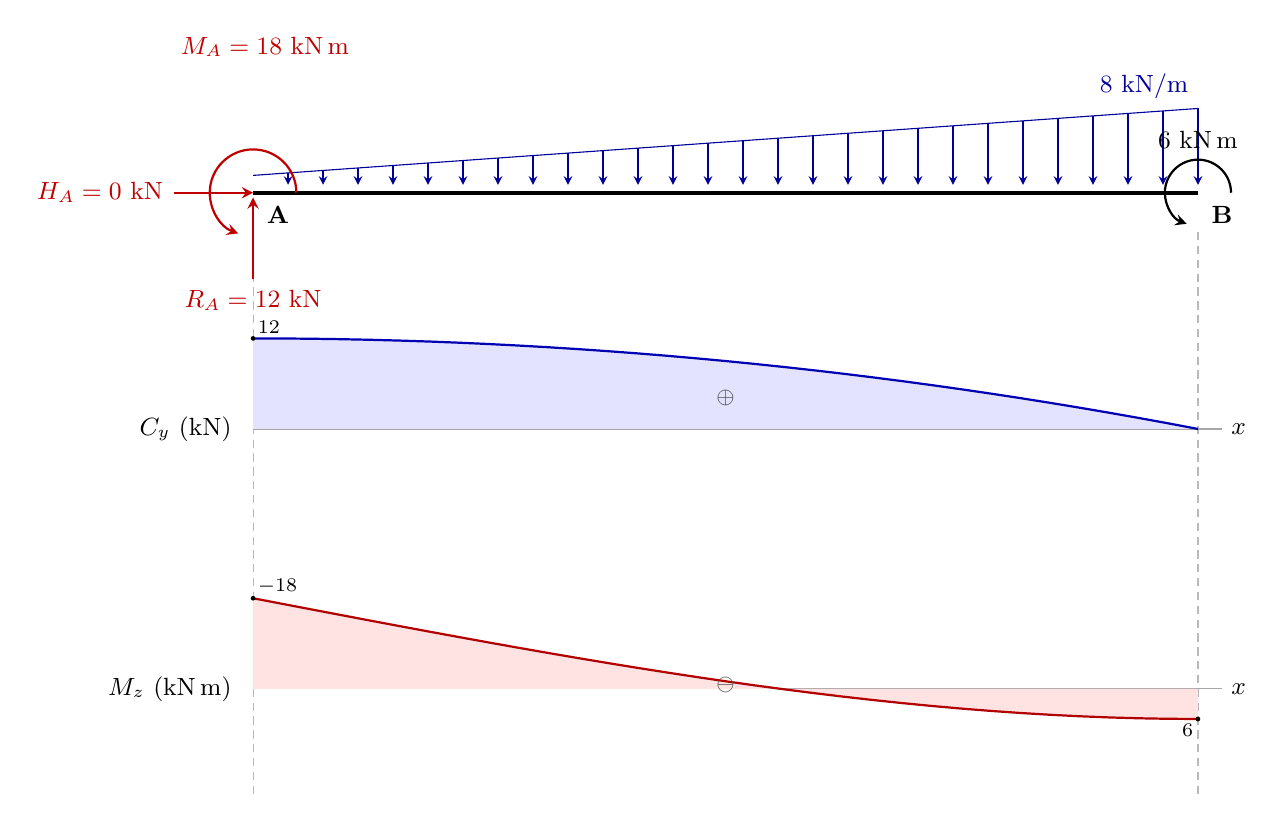
\begin{tikzpicture}
\draw[densely dashed,gray!55] (12.0000,-0.5000) -- (12.0000,-7.7000);
\draw[densely dashed,gray!55] (0.0000,-0.5000) -- (0.0000,-7.7000);
\draw[-stealth,blue!60!black] (0.4444,0.2515) -- (0.4444,0.1000);
\draw[-stealth,blue!60!black] (0.8889,0.2830) -- (0.8889,0.1000);
\draw[-stealth,blue!60!black] (1.3333,0.3144) -- (1.3333,0.1000);
\draw[-stealth,blue!60!black] (1.7778,0.3459) -- (1.7778,0.1000);
\draw[-stealth,blue!60!black] (2.2222,0.3774) -- (2.2222,0.1000);
\draw[-stealth,blue!60!black] (2.6667,0.4089) -- (2.6667,0.1000);
\draw[-stealth,blue!60!black] (3.1111,0.4404) -- (3.1111,0.1000);
\draw[-stealth,blue!60!black] (3.5556,0.4719) -- (3.5556,0.1000);
\draw[-stealth,blue!60!black] (4.0000,0.5033) -- (4.0000,0.1000);
\draw[-stealth,blue!60!black] (4.4444,0.5348) -- (4.4444,0.1000);
\draw[-stealth,blue!60!black] (4.8889,0.5663) -- (4.8889,0.1000);
\draw[-stealth,blue!60!black] (5.3333,0.5978) -- (5.3333,0.1000);
\draw[-stealth,blue!60!black] (5.7778,0.6293) -- (5.7778,0.1000);
\draw[-stealth,blue!60!black] (6.2222,0.6607) -- (6.2222,0.1000);
\draw[-stealth,blue!60!black] (6.6667,0.6922) -- (6.6667,0.1000);
\draw[-stealth,blue!60!black] (7.1111,0.7237) -- (7.1111,0.1000);
\draw[-stealth,blue!60!black] (7.5556,0.7552) -- (7.5556,0.1000);
\draw[-stealth,blue!60!black] (8.0000,0.7867) -- (8.0000,0.1000);
\draw[-stealth,blue!60!black] (8.4444,0.8181) -- (8.4444,0.1000);
\draw[-stealth,blue!60!black] (8.8889,0.8496) -- (8.8889,0.1000);
\draw[-stealth,blue!60!black] (9.3333,0.8811) -- (9.3333,0.1000);
\draw[-stealth,blue!60!black] (9.7778,0.9126) -- (9.7778,0.1000);
\draw[-stealth,blue!60!black] (10.2222,0.9441) -- (10.2222,0.1000);
\draw[-stealth,blue!60!black] (10.6667,0.9756) -- (10.6667,0.1000);
\draw[-stealth,blue!60!black] (11.1111,1.0070) -- (11.1111,0.1000);
\draw[-stealth,blue!60!black] (11.5556,1.0385) -- (11.5556,0.1000);
\draw[-stealth,blue!60!black] (12.0000,1.0700) -- (12.0000,0.1000);
% studium:at distributed 0 x=0 to=3 check=span
\draw[blue!60!black] (0.0000,0.2200) -- (0.4444,0.2515) -- (0.8889,0.2830) -- (1.3333,0.3144) -- (1.7778,0.3459) -- (2.2222,0.3774) -- (2.6667,0.4089) -- (3.1111,0.4404) -- (3.5556,0.4719) -- (4.0000,0.5033) -- (4.4444,0.5348) -- (4.8889,0.5663) -- (5.3333,0.5978) -- (5.7778,0.6293) -- (6.2222,0.6607) -- (6.6667,0.6922) -- (7.1111,0.7237) -- (7.5556,0.7552) -- (8.0000,0.7867) -- (8.4444,0.8181) -- (8.8889,0.8496) -- (9.3333,0.8811) -- (9.7778,0.9126) -- (10.2222,0.9441) -- (10.6667,0.9756) -- (11.1111,1.0070) -- (11.5556,1.0385) -- (12.0000,1.0700);
\node[font=\small,anchor=south east,blue!60!black] at (12.0000,1.0700) {$8$~\mbox{kN/m}};
\draw[line width=1.6pt] (0,0.0000) -- (12.0000,0.0000);
% studium:at couple 0 x=3 check=first
\node[font=\small,anchor=south,black] at (12.0000,0.4400) {$6$~\mbox{kN\,m}};
\draw[-stealth,thick,black] (12.4200,0.0000) arc (0:250:0.42);
% studium:reaction H_A value=0
% studium:at reaction H_A x=0 check=tip
\draw[-stealth,thick,red!75!black] (-1.0000,0.0000) -- (0.0000,0.0000);
\node[font=\small,anchor=east,red!75!black] at (-1.0200,0.0000) {$H_{A} = 0$~\mbox{kN}};
% studium:reaction R_A value=12
% studium:at reaction R_A x=0 check=tip
\draw[-stealth,thick,red!75!black] (0.0000,-1.1000) -- (0.0000,-0.0600);
\node[font=\small,anchor=north,red!75!black] at (0.0000,-1.1200) {$R_{A} = 12$~\mbox{kN}};
% studium:reaction M_A value=18
% studium:at reaction M_A x=0 check=arc
\draw[-stealth,thick,red!75!black] (0.5500,0.0000) arc (0:250:0.55);
\node[font=\small,anchor=south,red!75!black] at (0.1500,1.6000) {$M_{A} = 18$~\mbox{kN\,m}};
\node[font=\small\bfseries,anchor=north west] at (0.0500,-0.0500) {A};
\node[font=\small\bfseries,anchor=north west] at (12.0500,-0.0500) {B};
\draw[gray!70] (0,-3.0000) -- (12.3000,-3.0000);
\fill[blue!11] (0.0000,-3.0000) -- (0.0000,-1.8500) -- (0.3750,-1.8511) -- (0.7500,-1.8545) -- (1.1250,-1.8601) -- (1.5000,-1.8680) -- (1.8750,-1.8781) -- (2.2500,-1.8904) -- (2.6250,-1.9050) -- (3.0000,-1.9219) -- (3.3750,-1.9410) -- (3.7500,-1.9623) -- (4.1250,-1.9859) -- (4.5000,-2.0117) -- (4.8750,-2.0398) -- (5.2500,-2.0701) -- (5.6250,-2.1027) -- (6.0000,-2.1375) -- (6.3750,-2.1746) -- (6.7500,-2.2139) -- (7.1250,-2.2554) -- (7.5000,-2.2992) -- (7.8750,-2.3453) -- (8.2500,-2.3936) -- (8.6250,-2.4441) -- (9.0000,-2.4969) -- (9.3750,-2.5519) -- (9.7500,-2.6092) -- (10.1250,-2.6687) -- (10.5000,-2.7305) -- (10.8750,-2.7945) -- (11.2500,-2.8607) -- (11.6250,-2.9292) -- (12.0000,-3.0000) -- (12.0000,-3.0000) -- cycle;
% studium:series V sx=4.0 sy=0.09583333333333333 x0=0.0 y0=-3.0 sign=1
\draw[thick,blue!70!black] (0.0000,-1.8500) -- (0.3750,-1.8511) -- (0.7500,-1.8545) -- (1.1250,-1.8601) -- (1.5000,-1.8680) -- (1.8750,-1.8781) -- (2.2500,-1.8904) -- (2.6250,-1.9050) -- (3.0000,-1.9219) -- (3.3750,-1.9410) -- (3.7500,-1.9623) -- (4.1250,-1.9859) -- (4.5000,-2.0117) -- (4.8750,-2.0398) -- (5.2500,-2.0701) -- (5.6250,-2.1027) -- (6.0000,-2.1375) -- (6.3750,-2.1746) -- (6.7500,-2.2139) -- (7.1250,-2.2554) -- (7.5000,-2.2992) -- (7.8750,-2.3453) -- (8.2500,-2.3936) -- (8.6250,-2.4441) -- (9.0000,-2.4969) -- (9.3750,-2.5519) -- (9.7500,-2.6092) -- (10.1250,-2.6687) -- (10.5000,-2.7305) -- (10.8750,-2.7945) -- (11.2500,-2.8607) -- (11.6250,-2.9292) -- (12.0000,-3.0000);
% studium:end V
\node[font=\small,anchor=east] at (-0.15,-3.0000) {$C_y$ (kN)};
\node[font=\small,anchor=west] at (12.3000,-3.0000) {$x$};
% studium:label V x=0 side=right value=12
\fill (0.0000,-1.8500) circle (0.03);
\node[font=\scriptsize,anchor=south west,inner sep=1.5pt] at (0.0000,-1.8500) {$12$};
\node[font=\footnotesize,gray!60!black] at (6.0000,-2.6119) {$\oplus$};
\draw[gray!70] (0,-6.3000) -- (12.3000,-6.3000);
\fill[red!11] (0.0000,-6.3000) -- (0.0000,-5.1500) -- (0.3750,-5.2219) -- (0.7500,-5.2936) -- (1.1250,-5.3650) -- (1.5000,-5.4360) -- (1.8750,-5.5065) -- (2.2500,-5.5762) -- (2.6250,-5.6451) -- (3.0000,-5.7130) -- (3.3750,-5.7798) -- (3.7500,-5.8454) -- (4.1250,-5.9095) -- (4.5000,-5.9721) -- (4.8750,-6.0330) -- (5.2500,-6.0920) -- (5.6250,-6.1492) -- (6.0000,-6.2042) -- (6.3750,-6.2569) -- (6.7500,-6.3073) -- (7.1250,-6.3551) -- (7.5000,-6.4003) -- (7.8750,-6.4427) -- (8.2500,-6.4821) -- (8.6250,-6.5185) -- (9.0000,-6.5516) -- (9.3750,-6.5813) -- (9.7500,-6.6075) -- (10.1250,-6.6301) -- (10.5000,-6.6489) -- (10.8750,-6.6638) -- (11.2500,-6.6745) -- (11.6250,-6.6811) -- (12.0000,-6.6833) -- (12.0000,-6.3000) -- cycle;
% studium:series M sx=4.0 sy=0.06388888888888888 x0=0.0 y0=-6.3 sign=-1
\draw[thick,red!70!black] (0.0000,-5.1500) -- (0.3750,-5.2219) -- (0.7500,-5.2936) -- (1.1250,-5.3650) -- (1.5000,-5.4360) -- (1.8750,-5.5065) -- (2.2500,-5.5762) -- (2.6250,-5.6451) -- (3.0000,-5.7130) -- (3.3750,-5.7798) -- (3.7500,-5.8454) -- (4.1250,-5.9095) -- (4.5000,-5.9721) -- (4.8750,-6.0330) -- (5.2500,-6.0920) -- (5.6250,-6.1492) -- (6.0000,-6.2042) -- (6.3750,-6.2569) -- (6.7500,-6.3073) -- (7.1250,-6.3551) -- (7.5000,-6.4003) -- (7.8750,-6.4427) -- (8.2500,-6.4821) -- (8.6250,-6.5185) -- (9.0000,-6.5516) -- (9.3750,-6.5813) -- (9.7500,-6.6075) -- (10.1250,-6.6301) -- (10.5000,-6.6489) -- (10.8750,-6.6638) -- (11.2500,-6.6745) -- (11.6250,-6.6811) -- (12.0000,-6.6833);
% studium:end M
\node[font=\small,anchor=east] at (-0.15,-6.3000) {$M_z$ (kN\,m)};
\node[font=\small,anchor=west] at (12.3000,-6.3000) {$x$};
% studium:label M x=0 side=right value=-18
\fill (0.0000,-5.1500) circle (0.03);
\node[font=\scriptsize,anchor=south west,inner sep=1.5pt] at (0.0000,-5.1500) {$-18$};
% studium:label M x=3 side=left value=6
\fill (12.0000,-6.6833) circle (0.03);
\node[font=\scriptsize,anchor=north east,inner sep=1.5pt] at (12.0000,-6.6833) {$6$};
\node[font=\footnotesize,gray!60!black] at (6.0000,-6.2569) {$\ominus$};
\end{tikzpicture}}%
\else
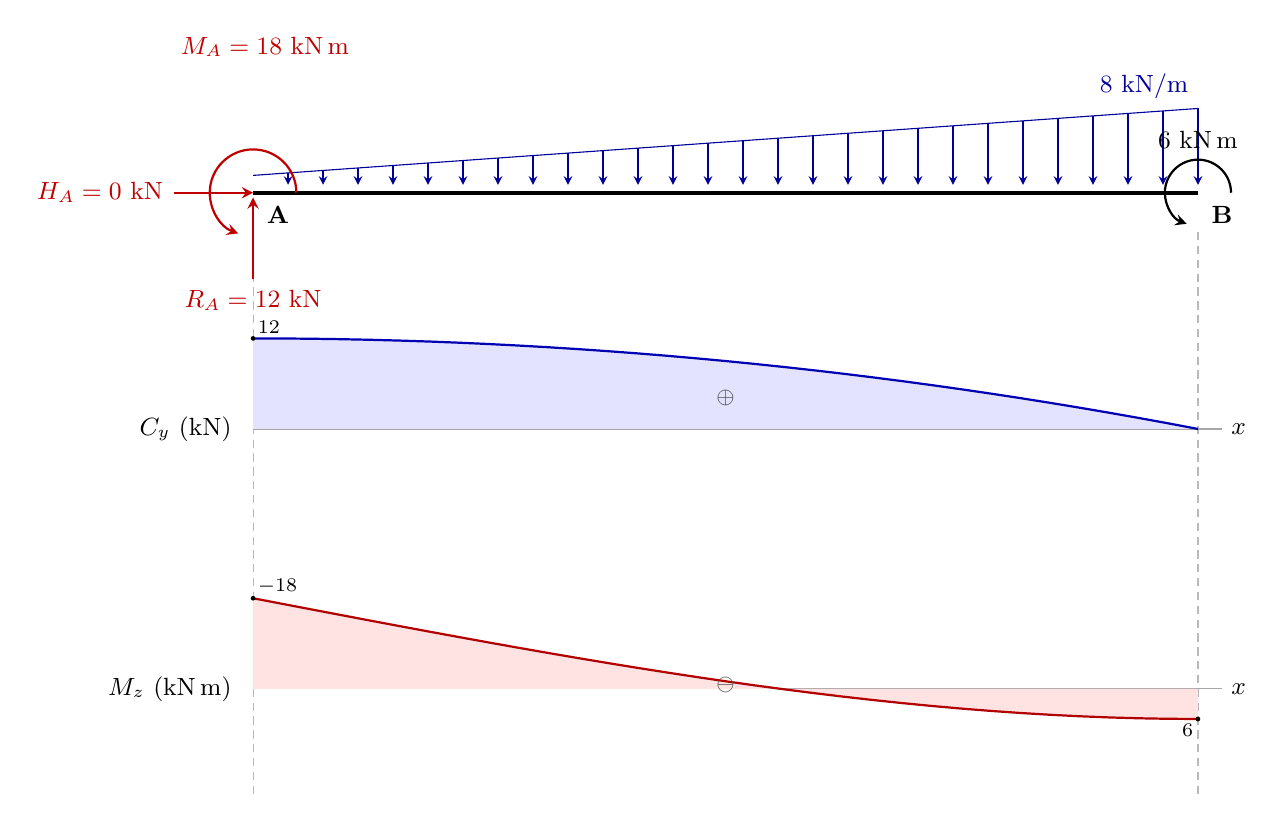
\begin{tikzpicture}
\draw[densely dashed,gray!55] (12.0000,-0.5000) -- (12.0000,-7.7000);
\draw[densely dashed,gray!55] (0.0000,-0.5000) -- (0.0000,-7.7000);
\draw[-stealth,blue!60!black] (0.4444,0.2515) -- (0.4444,0.1000);
\draw[-stealth,blue!60!black] (0.8889,0.2830) -- (0.8889,0.1000);
\draw[-stealth,blue!60!black] (1.3333,0.3144) -- (1.3333,0.1000);
\draw[-stealth,blue!60!black] (1.7778,0.3459) -- (1.7778,0.1000);
\draw[-stealth,blue!60!black] (2.2222,0.3774) -- (2.2222,0.1000);
\draw[-stealth,blue!60!black] (2.6667,0.4089) -- (2.6667,0.1000);
\draw[-stealth,blue!60!black] (3.1111,0.4404) -- (3.1111,0.1000);
\draw[-stealth,blue!60!black] (3.5556,0.4719) -- (3.5556,0.1000);
\draw[-stealth,blue!60!black] (4.0000,0.5033) -- (4.0000,0.1000);
\draw[-stealth,blue!60!black] (4.4444,0.5348) -- (4.4444,0.1000);
\draw[-stealth,blue!60!black] (4.8889,0.5663) -- (4.8889,0.1000);
\draw[-stealth,blue!60!black] (5.3333,0.5978) -- (5.3333,0.1000);
\draw[-stealth,blue!60!black] (5.7778,0.6293) -- (5.7778,0.1000);
\draw[-stealth,blue!60!black] (6.2222,0.6607) -- (6.2222,0.1000);
\draw[-stealth,blue!60!black] (6.6667,0.6922) -- (6.6667,0.1000);
\draw[-stealth,blue!60!black] (7.1111,0.7237) -- (7.1111,0.1000);
\draw[-stealth,blue!60!black] (7.5556,0.7552) -- (7.5556,0.1000);
\draw[-stealth,blue!60!black] (8.0000,0.7867) -- (8.0000,0.1000);
\draw[-stealth,blue!60!black] (8.4444,0.8181) -- (8.4444,0.1000);
\draw[-stealth,blue!60!black] (8.8889,0.8496) -- (8.8889,0.1000);
\draw[-stealth,blue!60!black] (9.3333,0.8811) -- (9.3333,0.1000);
\draw[-stealth,blue!60!black] (9.7778,0.9126) -- (9.7778,0.1000);
\draw[-stealth,blue!60!black] (10.2222,0.9441) -- (10.2222,0.1000);
\draw[-stealth,blue!60!black] (10.6667,0.9756) -- (10.6667,0.1000);
\draw[-stealth,blue!60!black] (11.1111,1.0070) -- (11.1111,0.1000);
\draw[-stealth,blue!60!black] (11.5556,1.0385) -- (11.5556,0.1000);
\draw[-stealth,blue!60!black] (12.0000,1.0700) -- (12.0000,0.1000);
% studium:at distributed 0 x=0 to=3 check=span
\draw[blue!60!black] (0.0000,0.2200) -- (0.4444,0.2515) -- (0.8889,0.2830) -- (1.3333,0.3144) -- (1.7778,0.3459) -- (2.2222,0.3774) -- (2.6667,0.4089) -- (3.1111,0.4404) -- (3.5556,0.4719) -- (4.0000,0.5033) -- (4.4444,0.5348) -- (4.8889,0.5663) -- (5.3333,0.5978) -- (5.7778,0.6293) -- (6.2222,0.6607) -- (6.6667,0.6922) -- (7.1111,0.7237) -- (7.5556,0.7552) -- (8.0000,0.7867) -- (8.4444,0.8181) -- (8.8889,0.8496) -- (9.3333,0.8811) -- (9.7778,0.9126) -- (10.2222,0.9441) -- (10.6667,0.9756) -- (11.1111,1.0070) -- (11.5556,1.0385) -- (12.0000,1.0700);
\node[font=\small,anchor=south east,blue!60!black] at (12.0000,1.0700) {$8$~\mbox{kN/m}};
\draw[line width=1.6pt] (0,0.0000) -- (12.0000,0.0000);
% studium:at couple 0 x=3 check=first
\node[font=\small,anchor=south,black] at (12.0000,0.4400) {$6$~\mbox{kN\,m}};
\draw[-stealth,thick,black] (12.4200,0.0000) arc (0:250:0.42);
% studium:reaction H_A value=0
% studium:at reaction H_A x=0 check=tip
\draw[-stealth,thick,red!75!black] (-1.0000,0.0000) -- (0.0000,0.0000);
\node[font=\small,anchor=east,red!75!black] at (-1.0200,0.0000) {$H_{A} = 0$~\mbox{kN}};
% studium:reaction R_A value=12
% studium:at reaction R_A x=0 check=tip
\draw[-stealth,thick,red!75!black] (0.0000,-1.1000) -- (0.0000,-0.0600);
\node[font=\small,anchor=north,red!75!black] at (0.0000,-1.1200) {$R_{A} = 12$~\mbox{kN}};
% studium:reaction M_A value=18
% studium:at reaction M_A x=0 check=arc
\draw[-stealth,thick,red!75!black] (0.5500,0.0000) arc (0:250:0.55);
\node[font=\small,anchor=south,red!75!black] at (0.1500,1.6000) {$M_{A} = 18$~\mbox{kN\,m}};
\node[font=\small\bfseries,anchor=north west] at (0.0500,-0.0500) {A};
\node[font=\small\bfseries,anchor=north west] at (12.0500,-0.0500) {B};
\draw[gray!70] (0,-3.0000) -- (12.3000,-3.0000);
\fill[blue!11] (0.0000,-3.0000) -- (0.0000,-1.8500) -- (0.3750,-1.8511) -- (0.7500,-1.8545) -- (1.1250,-1.8601) -- (1.5000,-1.8680) -- (1.8750,-1.8781) -- (2.2500,-1.8904) -- (2.6250,-1.9050) -- (3.0000,-1.9219) -- (3.3750,-1.9410) -- (3.7500,-1.9623) -- (4.1250,-1.9859) -- (4.5000,-2.0117) -- (4.8750,-2.0398) -- (5.2500,-2.0701) -- (5.6250,-2.1027) -- (6.0000,-2.1375) -- (6.3750,-2.1746) -- (6.7500,-2.2139) -- (7.1250,-2.2554) -- (7.5000,-2.2992) -- (7.8750,-2.3453) -- (8.2500,-2.3936) -- (8.6250,-2.4441) -- (9.0000,-2.4969) -- (9.3750,-2.5519) -- (9.7500,-2.6092) -- (10.1250,-2.6687) -- (10.5000,-2.7305) -- (10.8750,-2.7945) -- (11.2500,-2.8607) -- (11.6250,-2.9292) -- (12.0000,-3.0000) -- (12.0000,-3.0000) -- cycle;
% studium:series V sx=4.0 sy=0.09583333333333333 x0=0.0 y0=-3.0 sign=1
\draw[thick,blue!70!black] (0.0000,-1.8500) -- (0.3750,-1.8511) -- (0.7500,-1.8545) -- (1.1250,-1.8601) -- (1.5000,-1.8680) -- (1.8750,-1.8781) -- (2.2500,-1.8904) -- (2.6250,-1.9050) -- (3.0000,-1.9219) -- (3.3750,-1.9410) -- (3.7500,-1.9623) -- (4.1250,-1.9859) -- (4.5000,-2.0117) -- (4.8750,-2.0398) -- (5.2500,-2.0701) -- (5.6250,-2.1027) -- (6.0000,-2.1375) -- (6.3750,-2.1746) -- (6.7500,-2.2139) -- (7.1250,-2.2554) -- (7.5000,-2.2992) -- (7.8750,-2.3453) -- (8.2500,-2.3936) -- (8.6250,-2.4441) -- (9.0000,-2.4969) -- (9.3750,-2.5519) -- (9.7500,-2.6092) -- (10.1250,-2.6687) -- (10.5000,-2.7305) -- (10.8750,-2.7945) -- (11.2500,-2.8607) -- (11.6250,-2.9292) -- (12.0000,-3.0000);
% studium:end V
\node[font=\small,anchor=east] at (-0.15,-3.0000) {$C_y$ (kN)};
\node[font=\small,anchor=west] at (12.3000,-3.0000) {$x$};
% studium:label V x=0 side=right value=12
\fill (0.0000,-1.8500) circle (0.03);
\node[font=\scriptsize,anchor=south west,inner sep=1.5pt] at (0.0000,-1.8500) {$12$};
\node[font=\footnotesize,gray!60!black] at (6.0000,-2.6119) {$\oplus$};
\draw[gray!70] (0,-6.3000) -- (12.3000,-6.3000);
\fill[red!11] (0.0000,-6.3000) -- (0.0000,-5.1500) -- (0.3750,-5.2219) -- (0.7500,-5.2936) -- (1.1250,-5.3650) -- (1.5000,-5.4360) -- (1.8750,-5.5065) -- (2.2500,-5.5762) -- (2.6250,-5.6451) -- (3.0000,-5.7130) -- (3.3750,-5.7798) -- (3.7500,-5.8454) -- (4.1250,-5.9095) -- (4.5000,-5.9721) -- (4.8750,-6.0330) -- (5.2500,-6.0920) -- (5.6250,-6.1492) -- (6.0000,-6.2042) -- (6.3750,-6.2569) -- (6.7500,-6.3073) -- (7.1250,-6.3551) -- (7.5000,-6.4003) -- (7.8750,-6.4427) -- (8.2500,-6.4821) -- (8.6250,-6.5185) -- (9.0000,-6.5516) -- (9.3750,-6.5813) -- (9.7500,-6.6075) -- (10.1250,-6.6301) -- (10.5000,-6.6489) -- (10.8750,-6.6638) -- (11.2500,-6.6745) -- (11.6250,-6.6811) -- (12.0000,-6.6833) -- (12.0000,-6.3000) -- cycle;
% studium:series M sx=4.0 sy=0.06388888888888888 x0=0.0 y0=-6.3 sign=-1
\draw[thick,red!70!black] (0.0000,-5.1500) -- (0.3750,-5.2219) -- (0.7500,-5.2936) -- (1.1250,-5.3650) -- (1.5000,-5.4360) -- (1.8750,-5.5065) -- (2.2500,-5.5762) -- (2.6250,-5.6451) -- (3.0000,-5.7130) -- (3.3750,-5.7798) -- (3.7500,-5.8454) -- (4.1250,-5.9095) -- (4.5000,-5.9721) -- (4.8750,-6.0330) -- (5.2500,-6.0920) -- (5.6250,-6.1492) -- (6.0000,-6.2042) -- (6.3750,-6.2569) -- (6.7500,-6.3073) -- (7.1250,-6.3551) -- (7.5000,-6.4003) -- (7.8750,-6.4427) -- (8.2500,-6.4821) -- (8.6250,-6.5185) -- (9.0000,-6.5516) -- (9.3750,-6.5813) -- (9.7500,-6.6075) -- (10.1250,-6.6301) -- (10.5000,-6.6489) -- (10.8750,-6.6638) -- (11.2500,-6.6745) -- (11.6250,-6.6811) -- (12.0000,-6.6833);
% studium:end M
\node[font=\small,anchor=east] at (-0.15,-6.3000) {$M_z$ (kN\,m)};
\node[font=\small,anchor=west] at (12.3000,-6.3000) {$x$};
% studium:label M x=0 side=right value=-18
\fill (0.0000,-5.1500) circle (0.03);
\node[font=\scriptsize,anchor=south west,inner sep=1.5pt] at (0.0000,-5.1500) {$-18$};
% studium:label M x=3 side=left value=6
\fill (12.0000,-6.6833) circle (0.03);
\node[font=\scriptsize,anchor=north east,inner sep=1.5pt] at (12.0000,-6.6833) {$6$};
\node[font=\footnotesize,gray!60!black] at (6.0000,-6.2569) {$\ominus$};
\end{tikzpicture}%
\fi
\fi
\endgroup
\par\nopagebreak
\studiumcaption{fig:e2-c03-mens-esfuerzos}{Diagramas de la ménsula: cortante parabólico que se anula en el extremo libre y flector cúbico que cambia de signo.}
\end{minipage}\par\medskip

\textbf{Resultado e interpretación.}\[\fitmath{R_A = 12\ \mathrm{kN},\qquad M_z(0) = -18\ \mathrm{kN\,m},\qquad M_z(3) = 6\ \mathrm{kN\,m}}\]

El flector cambia de signo a lo largo de la ménsula: cerca del empotramiento domina la carga, que tracciona la fibra superior, y cerca del extremo domina el momento antihorario, que comprime la fibra superior. El cortante no cambia de signo, de modo que el flector es monótono y sus extremos están en los bordes de la barra.

\par\textbf{Comprobación.} Recalcula los pasos con unidades coherentes y aplica el control específico indicado en la orientación del capítulo.

\textbf{Límites.}\begin{itemize}\item no se incluye el peso propio\end{itemize}

\textbf{Errores frecuentes.}\begin{itemize}\item aplicar la resultante de la carga triangular en el centro de la ménsula
\item olvidar que un momento aplicado en el extremo libre fija el valor del flector en ese extremo
\item dibujar el flector negativo hacia abajo\end{itemize}

\end{studiumworked}

\Needspace{.3\textheight}

\begin{studiumworked}{PRB-0199}

\section{PRB-0199 · Reacciones y flectores extremos}

\textbf{Enunciado.} Una viga $A B C$ de 7 m tiene un apoyo fijo en $A$ y un apoyo móvil en $B$, a 5 m de $A$, y vuela 2 m hasta $C$. Soporta una carga uniforme de 6 kN/m hacia abajo entre $A$ y $B$, un momento horario de 12 kN$\cdot$m en el punto medio $D$ de $AB$ y una carga puntual de 10 kN hacia abajo en $C$. Calcule las reacciones, dibuje los diagramas de cortantes y flectores e indique el flector máximo positivo y el negativo.

\par\medskip\noindent\begin{tabular}{@{}p{.18\linewidth}p{.26\linewidth}p{.48\linewidth}@{}}
\toprule Símbolo & Valor y unidad & Significado\\\midrule
$q$ & $6\,\mathrm{kN/m}$ & carga uniforme en AB\\
$M_{D}$ & $12\,\mathrm{kN\,m}$ & momento horario en D\\
$P$ & $10\,\mathrm{kN}$ & carga en el voladizo\\
\bottomrule\end{tabular}\par\medskip

\par\medskip\noindent\begin{minipage}{\linewidth}
\centering
\begingroup
\setbox0=\hbox{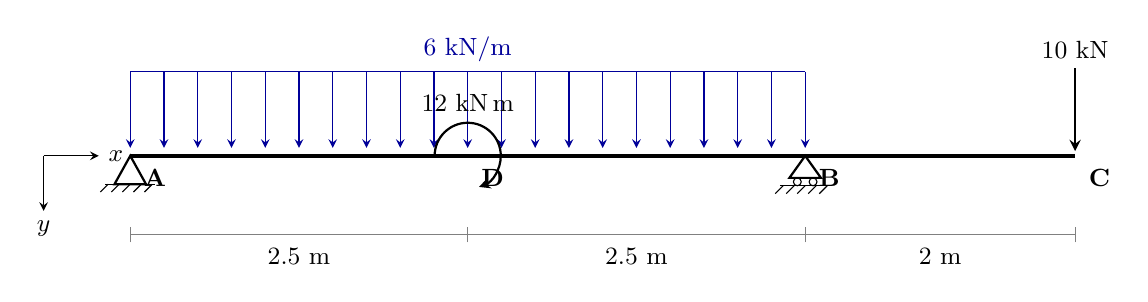
\begin{tikzpicture}
\draw[-stealth,blue!60!black] (0.0000,1.0700) -- (0.0000,0.1000);
\draw[-stealth,blue!60!black] (0.4286,1.0700) -- (0.4286,0.1000);
\draw[-stealth,blue!60!black] (0.8571,1.0700) -- (0.8571,0.1000);
\draw[-stealth,blue!60!black] (1.2857,1.0700) -- (1.2857,0.1000);
\draw[-stealth,blue!60!black] (1.7143,1.0700) -- (1.7143,0.1000);
\draw[-stealth,blue!60!black] (2.1429,1.0700) -- (2.1429,0.1000);
\draw[-stealth,blue!60!black] (2.5714,1.0700) -- (2.5714,0.1000);
\draw[-stealth,blue!60!black] (3.0000,1.0700) -- (3.0000,0.1000);
\draw[-stealth,blue!60!black] (3.4286,1.0700) -- (3.4286,0.1000);
\draw[-stealth,blue!60!black] (3.8571,1.0700) -- (3.8571,0.1000);
\draw[-stealth,blue!60!black] (4.2857,1.0700) -- (4.2857,0.1000);
\draw[-stealth,blue!60!black] (4.7143,1.0700) -- (4.7143,0.1000);
\draw[-stealth,blue!60!black] (5.1429,1.0700) -- (5.1429,0.1000);
\draw[-stealth,blue!60!black] (5.5714,1.0700) -- (5.5714,0.1000);
\draw[-stealth,blue!60!black] (6.0000,1.0700) -- (6.0000,0.1000);
\draw[-stealth,blue!60!black] (6.4286,1.0700) -- (6.4286,0.1000);
\draw[-stealth,blue!60!black] (6.8571,1.0700) -- (6.8571,0.1000);
\draw[-stealth,blue!60!black] (7.2857,1.0700) -- (7.2857,0.1000);
\draw[-stealth,blue!60!black] (7.7143,1.0700) -- (7.7143,0.1000);
\draw[-stealth,blue!60!black] (8.1429,1.0700) -- (8.1429,0.1000);
\draw[-stealth,blue!60!black] (8.5714,1.0700) -- (8.5714,0.1000);
% studium:at distributed 0 x=0 to=5 check=span
\draw[blue!60!black] (0.0000,1.0700) -- (0.4286,1.0700) -- (0.8571,1.0700) -- (1.2857,1.0700) -- (1.7143,1.0700) -- (2.1429,1.0700) -- (2.5714,1.0700) -- (3.0000,1.0700) -- (3.4286,1.0700) -- (3.8571,1.0700) -- (4.2857,1.0700) -- (4.7143,1.0700) -- (5.1429,1.0700) -- (5.5714,1.0700) -- (6.0000,1.0700) -- (6.4286,1.0700) -- (6.8571,1.0700) -- (7.2857,1.0700) -- (7.7143,1.0700) -- (8.1429,1.0700) -- (8.5714,1.0700);
\node[font=\small,anchor=south,blue!60!black] at (4.2857,1.0700) {$6$~\mbox{kN/m}};
\draw[line width=1.6pt] (0,0.0000) -- (12.0000,0.0000);
% studium:at support A x=0 check=first
\draw[thick,fill=white] (0.0000,0.0000) -- (-0.2000,-0.3600) -- (0.2000,-0.3600) -- cycle;
\draw (-0.3200,-0.3600) -- (0.3200,-0.3600);
\draw (-0.2800,-0.3600) -- (-0.3800,-0.4600);
\draw (-0.1400,-0.3600) -- (-0.2400,-0.4600);
\draw (0.0000,-0.3600) -- (-0.1000,-0.4600);
\draw (0.1400,-0.3600) -- (0.0400,-0.4600);
\draw (0.2800,-0.3600) -- (0.1800,-0.4600);
% studium:at support B x=5 check=first
\draw[thick,fill=white] (8.5714,0.0000) -- (8.3714,-0.2800) -- (8.7714,-0.2800) -- cycle;
\draw (8.4714,-0.3300) circle (0.05);
\draw (8.6714,-0.3300) circle (0.05);
\draw (8.2514,-0.3800) -- (8.8914,-0.3800);
\draw (8.2914,-0.3800) -- (8.1914,-0.4800);
\draw (8.4314,-0.3800) -- (8.3314,-0.4800);
\draw (8.5714,-0.3800) -- (8.4714,-0.4800);
\draw (8.7114,-0.3800) -- (8.6114,-0.4800);
\draw (8.8514,-0.3800) -- (8.7514,-0.4800);
% studium:at force 0 x=7 check=tip
\draw[-stealth,thick,black] (12.0000,1.1100) -- (12.0000,0.0600);
\node[font=\small,anchor=south] at (12.0000,1.1100) {$10$~\mbox{kN}};
% studium:at couple 0 x=5/2 check=first
\node[font=\small,anchor=south,black] at (4.2857,0.4400) {$12$~\mbox{kN\,m}};
\draw[-stealth,thick,black] (3.8657,0.0000) arc (180:-70:0.42);
\node[font=\small\bfseries,anchor=north west] at (0.0500,-0.0500) {A};
\node[font=\small\bfseries,anchor=north west] at (4.3357,-0.0500) {D};
\node[font=\small\bfseries,anchor=north west] at (8.6214,-0.0500) {B};
\node[font=\small\bfseries,anchor=north west] at (12.0500,-0.0500) {C};
\draw[gray] (0,-1.0000) -- (12.0000,-1.0000);
\draw[gray] (0.0000,-1.1000) -- (0.0000,-0.9000);
\draw[gray] (4.2857,-1.1000) -- (4.2857,-0.9000);
\draw[gray] (8.5714,-1.1000) -- (8.5714,-0.9000);
\draw[gray] (12.0000,-1.1000) -- (12.0000,-0.9000);
\node[font=\small,anchor=north] at (2.1429,-1.0500) {$2.5$~\mbox{m}};
\node[font=\small,anchor=north] at (6.4286,-1.0500) {$2.5$~\mbox{m}};
\node[font=\small,anchor=north] at (10.2857,-1.0500) {$2$~\mbox{m}};
\draw[-stealth] (-1.1,0.0000) -- (-0.4,0.0000) node[right,font=\small] {$x$};
\draw[-stealth] (-1.1,0.0000) -- (-1.1,-0.7000) node[below,font=\small] {$y$};
\end{tikzpicture}}%
\count0=\ht0
\advance\count0 by \dp0
\count2=\wd0
\count4=\dimexpr\textheight/100*38\relax
\count6=\linewidth
\ifnum\count0<1
\count0=1
\fi
\ifnum\count2<1
\count2=1
\fi
\divide\count0 by 4096
\divide\count2 by 4096
\divide\count4 by 4096
\divide\count6 by 4096
\ifnum\count0<1
\count0=1
\fi
\ifnum\count2<1
\count2=1
\fi
\ifnum\count4<1
\count4=1
\fi
\ifnum\count6<1
\count6=1
\fi
\count8=\count2
\ifnum\count0>\count4
\count8=\numexpr\count2*\count4/\count0\relax
\fi
\ifnum\count8>\count6
\resizebox{\linewidth}{!}{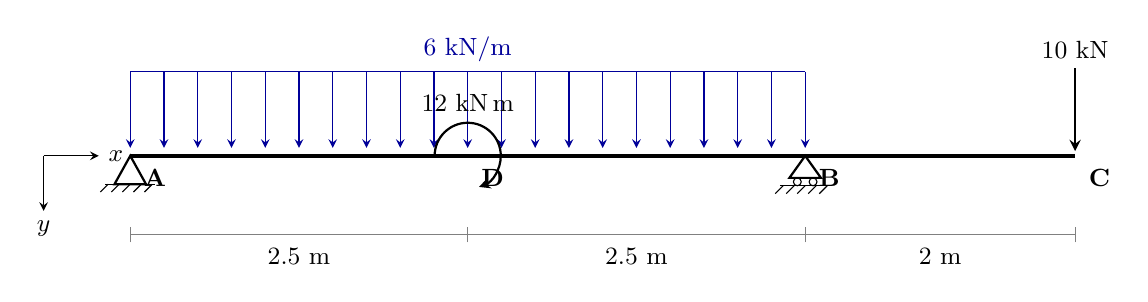
\begin{tikzpicture}
\draw[-stealth,blue!60!black] (0.0000,1.0700) -- (0.0000,0.1000);
\draw[-stealth,blue!60!black] (0.4286,1.0700) -- (0.4286,0.1000);
\draw[-stealth,blue!60!black] (0.8571,1.0700) -- (0.8571,0.1000);
\draw[-stealth,blue!60!black] (1.2857,1.0700) -- (1.2857,0.1000);
\draw[-stealth,blue!60!black] (1.7143,1.0700) -- (1.7143,0.1000);
\draw[-stealth,blue!60!black] (2.1429,1.0700) -- (2.1429,0.1000);
\draw[-stealth,blue!60!black] (2.5714,1.0700) -- (2.5714,0.1000);
\draw[-stealth,blue!60!black] (3.0000,1.0700) -- (3.0000,0.1000);
\draw[-stealth,blue!60!black] (3.4286,1.0700) -- (3.4286,0.1000);
\draw[-stealth,blue!60!black] (3.8571,1.0700) -- (3.8571,0.1000);
\draw[-stealth,blue!60!black] (4.2857,1.0700) -- (4.2857,0.1000);
\draw[-stealth,blue!60!black] (4.7143,1.0700) -- (4.7143,0.1000);
\draw[-stealth,blue!60!black] (5.1429,1.0700) -- (5.1429,0.1000);
\draw[-stealth,blue!60!black] (5.5714,1.0700) -- (5.5714,0.1000);
\draw[-stealth,blue!60!black] (6.0000,1.0700) -- (6.0000,0.1000);
\draw[-stealth,blue!60!black] (6.4286,1.0700) -- (6.4286,0.1000);
\draw[-stealth,blue!60!black] (6.8571,1.0700) -- (6.8571,0.1000);
\draw[-stealth,blue!60!black] (7.2857,1.0700) -- (7.2857,0.1000);
\draw[-stealth,blue!60!black] (7.7143,1.0700) -- (7.7143,0.1000);
\draw[-stealth,blue!60!black] (8.1429,1.0700) -- (8.1429,0.1000);
\draw[-stealth,blue!60!black] (8.5714,1.0700) -- (8.5714,0.1000);
% studium:at distributed 0 x=0 to=5 check=span
\draw[blue!60!black] (0.0000,1.0700) -- (0.4286,1.0700) -- (0.8571,1.0700) -- (1.2857,1.0700) -- (1.7143,1.0700) -- (2.1429,1.0700) -- (2.5714,1.0700) -- (3.0000,1.0700) -- (3.4286,1.0700) -- (3.8571,1.0700) -- (4.2857,1.0700) -- (4.7143,1.0700) -- (5.1429,1.0700) -- (5.5714,1.0700) -- (6.0000,1.0700) -- (6.4286,1.0700) -- (6.8571,1.0700) -- (7.2857,1.0700) -- (7.7143,1.0700) -- (8.1429,1.0700) -- (8.5714,1.0700);
\node[font=\small,anchor=south,blue!60!black] at (4.2857,1.0700) {$6$~\mbox{kN/m}};
\draw[line width=1.6pt] (0,0.0000) -- (12.0000,0.0000);
% studium:at support A x=0 check=first
\draw[thick,fill=white] (0.0000,0.0000) -- (-0.2000,-0.3600) -- (0.2000,-0.3600) -- cycle;
\draw (-0.3200,-0.3600) -- (0.3200,-0.3600);
\draw (-0.2800,-0.3600) -- (-0.3800,-0.4600);
\draw (-0.1400,-0.3600) -- (-0.2400,-0.4600);
\draw (0.0000,-0.3600) -- (-0.1000,-0.4600);
\draw (0.1400,-0.3600) -- (0.0400,-0.4600);
\draw (0.2800,-0.3600) -- (0.1800,-0.4600);
% studium:at support B x=5 check=first
\draw[thick,fill=white] (8.5714,0.0000) -- (8.3714,-0.2800) -- (8.7714,-0.2800) -- cycle;
\draw (8.4714,-0.3300) circle (0.05);
\draw (8.6714,-0.3300) circle (0.05);
\draw (8.2514,-0.3800) -- (8.8914,-0.3800);
\draw (8.2914,-0.3800) -- (8.1914,-0.4800);
\draw (8.4314,-0.3800) -- (8.3314,-0.4800);
\draw (8.5714,-0.3800) -- (8.4714,-0.4800);
\draw (8.7114,-0.3800) -- (8.6114,-0.4800);
\draw (8.8514,-0.3800) -- (8.7514,-0.4800);
% studium:at force 0 x=7 check=tip
\draw[-stealth,thick,black] (12.0000,1.1100) -- (12.0000,0.0600);
\node[font=\small,anchor=south] at (12.0000,1.1100) {$10$~\mbox{kN}};
% studium:at couple 0 x=5/2 check=first
\node[font=\small,anchor=south,black] at (4.2857,0.4400) {$12$~\mbox{kN\,m}};
\draw[-stealth,thick,black] (3.8657,0.0000) arc (180:-70:0.42);
\node[font=\small\bfseries,anchor=north west] at (0.0500,-0.0500) {A};
\node[font=\small\bfseries,anchor=north west] at (4.3357,-0.0500) {D};
\node[font=\small\bfseries,anchor=north west] at (8.6214,-0.0500) {B};
\node[font=\small\bfseries,anchor=north west] at (12.0500,-0.0500) {C};
\draw[gray] (0,-1.0000) -- (12.0000,-1.0000);
\draw[gray] (0.0000,-1.1000) -- (0.0000,-0.9000);
\draw[gray] (4.2857,-1.1000) -- (4.2857,-0.9000);
\draw[gray] (8.5714,-1.1000) -- (8.5714,-0.9000);
\draw[gray] (12.0000,-1.1000) -- (12.0000,-0.9000);
\node[font=\small,anchor=north] at (2.1429,-1.0500) {$2.5$~\mbox{m}};
\node[font=\small,anchor=north] at (6.4286,-1.0500) {$2.5$~\mbox{m}};
\node[font=\small,anchor=north] at (10.2857,-1.0500) {$2$~\mbox{m}};
\draw[-stealth] (-1.1,0.0000) -- (-0.4,0.0000) node[right,font=\small] {$x$};
\draw[-stealth] (-1.1,0.0000) -- (-1.1,-0.7000) node[below,font=\small] {$y$};
\end{tikzpicture}}%
\else
\ifnum\count0>\count4
\resizebox{!}{\dimexpr\textheight/100*38\relax}{\begin{tikzpicture}
\draw[-stealth,blue!60!black] (0.0000,1.0700) -- (0.0000,0.1000);
\draw[-stealth,blue!60!black] (0.4286,1.0700) -- (0.4286,0.1000);
\draw[-stealth,blue!60!black] (0.8571,1.0700) -- (0.8571,0.1000);
\draw[-stealth,blue!60!black] (1.2857,1.0700) -- (1.2857,0.1000);
\draw[-stealth,blue!60!black] (1.7143,1.0700) -- (1.7143,0.1000);
\draw[-stealth,blue!60!black] (2.1429,1.0700) -- (2.1429,0.1000);
\draw[-stealth,blue!60!black] (2.5714,1.0700) -- (2.5714,0.1000);
\draw[-stealth,blue!60!black] (3.0000,1.0700) -- (3.0000,0.1000);
\draw[-stealth,blue!60!black] (3.4286,1.0700) -- (3.4286,0.1000);
\draw[-stealth,blue!60!black] (3.8571,1.0700) -- (3.8571,0.1000);
\draw[-stealth,blue!60!black] (4.2857,1.0700) -- (4.2857,0.1000);
\draw[-stealth,blue!60!black] (4.7143,1.0700) -- (4.7143,0.1000);
\draw[-stealth,blue!60!black] (5.1429,1.0700) -- (5.1429,0.1000);
\draw[-stealth,blue!60!black] (5.5714,1.0700) -- (5.5714,0.1000);
\draw[-stealth,blue!60!black] (6.0000,1.0700) -- (6.0000,0.1000);
\draw[-stealth,blue!60!black] (6.4286,1.0700) -- (6.4286,0.1000);
\draw[-stealth,blue!60!black] (6.8571,1.0700) -- (6.8571,0.1000);
\draw[-stealth,blue!60!black] (7.2857,1.0700) -- (7.2857,0.1000);
\draw[-stealth,blue!60!black] (7.7143,1.0700) -- (7.7143,0.1000);
\draw[-stealth,blue!60!black] (8.1429,1.0700) -- (8.1429,0.1000);
\draw[-stealth,blue!60!black] (8.5714,1.0700) -- (8.5714,0.1000);
% studium:at distributed 0 x=0 to=5 check=span
\draw[blue!60!black] (0.0000,1.0700) -- (0.4286,1.0700) -- (0.8571,1.0700) -- (1.2857,1.0700) -- (1.7143,1.0700) -- (2.1429,1.0700) -- (2.5714,1.0700) -- (3.0000,1.0700) -- (3.4286,1.0700) -- (3.8571,1.0700) -- (4.2857,1.0700) -- (4.7143,1.0700) -- (5.1429,1.0700) -- (5.5714,1.0700) -- (6.0000,1.0700) -- (6.4286,1.0700) -- (6.8571,1.0700) -- (7.2857,1.0700) -- (7.7143,1.0700) -- (8.1429,1.0700) -- (8.5714,1.0700);
\node[font=\small,anchor=south,blue!60!black] at (4.2857,1.0700) {$6$~\mbox{kN/m}};
\draw[line width=1.6pt] (0,0.0000) -- (12.0000,0.0000);
% studium:at support A x=0 check=first
\draw[thick,fill=white] (0.0000,0.0000) -- (-0.2000,-0.3600) -- (0.2000,-0.3600) -- cycle;
\draw (-0.3200,-0.3600) -- (0.3200,-0.3600);
\draw (-0.2800,-0.3600) -- (-0.3800,-0.4600);
\draw (-0.1400,-0.3600) -- (-0.2400,-0.4600);
\draw (0.0000,-0.3600) -- (-0.1000,-0.4600);
\draw (0.1400,-0.3600) -- (0.0400,-0.4600);
\draw (0.2800,-0.3600) -- (0.1800,-0.4600);
% studium:at support B x=5 check=first
\draw[thick,fill=white] (8.5714,0.0000) -- (8.3714,-0.2800) -- (8.7714,-0.2800) -- cycle;
\draw (8.4714,-0.3300) circle (0.05);
\draw (8.6714,-0.3300) circle (0.05);
\draw (8.2514,-0.3800) -- (8.8914,-0.3800);
\draw (8.2914,-0.3800) -- (8.1914,-0.4800);
\draw (8.4314,-0.3800) -- (8.3314,-0.4800);
\draw (8.5714,-0.3800) -- (8.4714,-0.4800);
\draw (8.7114,-0.3800) -- (8.6114,-0.4800);
\draw (8.8514,-0.3800) -- (8.7514,-0.4800);
% studium:at force 0 x=7 check=tip
\draw[-stealth,thick,black] (12.0000,1.1100) -- (12.0000,0.0600);
\node[font=\small,anchor=south] at (12.0000,1.1100) {$10$~\mbox{kN}};
% studium:at couple 0 x=5/2 check=first
\node[font=\small,anchor=south,black] at (4.2857,0.4400) {$12$~\mbox{kN\,m}};
\draw[-stealth,thick,black] (3.8657,0.0000) arc (180:-70:0.42);
\node[font=\small\bfseries,anchor=north west] at (0.0500,-0.0500) {A};
\node[font=\small\bfseries,anchor=north west] at (4.3357,-0.0500) {D};
\node[font=\small\bfseries,anchor=north west] at (8.6214,-0.0500) {B};
\node[font=\small\bfseries,anchor=north west] at (12.0500,-0.0500) {C};
\draw[gray] (0,-1.0000) -- (12.0000,-1.0000);
\draw[gray] (0.0000,-1.1000) -- (0.0000,-0.9000);
\draw[gray] (4.2857,-1.1000) -- (4.2857,-0.9000);
\draw[gray] (8.5714,-1.1000) -- (8.5714,-0.9000);
\draw[gray] (12.0000,-1.1000) -- (12.0000,-0.9000);
\node[font=\small,anchor=north] at (2.1429,-1.0500) {$2.5$~\mbox{m}};
\node[font=\small,anchor=north] at (6.4286,-1.0500) {$2.5$~\mbox{m}};
\node[font=\small,anchor=north] at (10.2857,-1.0500) {$2$~\mbox{m}};
\draw[-stealth] (-1.1,0.0000) -- (-0.4,0.0000) node[right,font=\small] {$x$};
\draw[-stealth] (-1.1,0.0000) -- (-1.1,-0.7000) node[below,font=\small] {$y$};
\end{tikzpicture}}%
\else
\begin{tikzpicture}
\draw[-stealth,blue!60!black] (0.0000,1.0700) -- (0.0000,0.1000);
\draw[-stealth,blue!60!black] (0.4286,1.0700) -- (0.4286,0.1000);
\draw[-stealth,blue!60!black] (0.8571,1.0700) -- (0.8571,0.1000);
\draw[-stealth,blue!60!black] (1.2857,1.0700) -- (1.2857,0.1000);
\draw[-stealth,blue!60!black] (1.7143,1.0700) -- (1.7143,0.1000);
\draw[-stealth,blue!60!black] (2.1429,1.0700) -- (2.1429,0.1000);
\draw[-stealth,blue!60!black] (2.5714,1.0700) -- (2.5714,0.1000);
\draw[-stealth,blue!60!black] (3.0000,1.0700) -- (3.0000,0.1000);
\draw[-stealth,blue!60!black] (3.4286,1.0700) -- (3.4286,0.1000);
\draw[-stealth,blue!60!black] (3.8571,1.0700) -- (3.8571,0.1000);
\draw[-stealth,blue!60!black] (4.2857,1.0700) -- (4.2857,0.1000);
\draw[-stealth,blue!60!black] (4.7143,1.0700) -- (4.7143,0.1000);
\draw[-stealth,blue!60!black] (5.1429,1.0700) -- (5.1429,0.1000);
\draw[-stealth,blue!60!black] (5.5714,1.0700) -- (5.5714,0.1000);
\draw[-stealth,blue!60!black] (6.0000,1.0700) -- (6.0000,0.1000);
\draw[-stealth,blue!60!black] (6.4286,1.0700) -- (6.4286,0.1000);
\draw[-stealth,blue!60!black] (6.8571,1.0700) -- (6.8571,0.1000);
\draw[-stealth,blue!60!black] (7.2857,1.0700) -- (7.2857,0.1000);
\draw[-stealth,blue!60!black] (7.7143,1.0700) -- (7.7143,0.1000);
\draw[-stealth,blue!60!black] (8.1429,1.0700) -- (8.1429,0.1000);
\draw[-stealth,blue!60!black] (8.5714,1.0700) -- (8.5714,0.1000);
% studium:at distributed 0 x=0 to=5 check=span
\draw[blue!60!black] (0.0000,1.0700) -- (0.4286,1.0700) -- (0.8571,1.0700) -- (1.2857,1.0700) -- (1.7143,1.0700) -- (2.1429,1.0700) -- (2.5714,1.0700) -- (3.0000,1.0700) -- (3.4286,1.0700) -- (3.8571,1.0700) -- (4.2857,1.0700) -- (4.7143,1.0700) -- (5.1429,1.0700) -- (5.5714,1.0700) -- (6.0000,1.0700) -- (6.4286,1.0700) -- (6.8571,1.0700) -- (7.2857,1.0700) -- (7.7143,1.0700) -- (8.1429,1.0700) -- (8.5714,1.0700);
\node[font=\small,anchor=south,blue!60!black] at (4.2857,1.0700) {$6$~\mbox{kN/m}};
\draw[line width=1.6pt] (0,0.0000) -- (12.0000,0.0000);
% studium:at support A x=0 check=first
\draw[thick,fill=white] (0.0000,0.0000) -- (-0.2000,-0.3600) -- (0.2000,-0.3600) -- cycle;
\draw (-0.3200,-0.3600) -- (0.3200,-0.3600);
\draw (-0.2800,-0.3600) -- (-0.3800,-0.4600);
\draw (-0.1400,-0.3600) -- (-0.2400,-0.4600);
\draw (0.0000,-0.3600) -- (-0.1000,-0.4600);
\draw (0.1400,-0.3600) -- (0.0400,-0.4600);
\draw (0.2800,-0.3600) -- (0.1800,-0.4600);
% studium:at support B x=5 check=first
\draw[thick,fill=white] (8.5714,0.0000) -- (8.3714,-0.2800) -- (8.7714,-0.2800) -- cycle;
\draw (8.4714,-0.3300) circle (0.05);
\draw (8.6714,-0.3300) circle (0.05);
\draw (8.2514,-0.3800) -- (8.8914,-0.3800);
\draw (8.2914,-0.3800) -- (8.1914,-0.4800);
\draw (8.4314,-0.3800) -- (8.3314,-0.4800);
\draw (8.5714,-0.3800) -- (8.4714,-0.4800);
\draw (8.7114,-0.3800) -- (8.6114,-0.4800);
\draw (8.8514,-0.3800) -- (8.7514,-0.4800);
% studium:at force 0 x=7 check=tip
\draw[-stealth,thick,black] (12.0000,1.1100) -- (12.0000,0.0600);
\node[font=\small,anchor=south] at (12.0000,1.1100) {$10$~\mbox{kN}};
% studium:at couple 0 x=5/2 check=first
\node[font=\small,anchor=south,black] at (4.2857,0.4400) {$12$~\mbox{kN\,m}};
\draw[-stealth,thick,black] (3.8657,0.0000) arc (180:-70:0.42);
\node[font=\small\bfseries,anchor=north west] at (0.0500,-0.0500) {A};
\node[font=\small\bfseries,anchor=north west] at (4.3357,-0.0500) {D};
\node[font=\small\bfseries,anchor=north west] at (8.6214,-0.0500) {B};
\node[font=\small\bfseries,anchor=north west] at (12.0500,-0.0500) {C};
\draw[gray] (0,-1.0000) -- (12.0000,-1.0000);
\draw[gray] (0.0000,-1.1000) -- (0.0000,-0.9000);
\draw[gray] (4.2857,-1.1000) -- (4.2857,-0.9000);
\draw[gray] (8.5714,-1.1000) -- (8.5714,-0.9000);
\draw[gray] (12.0000,-1.1000) -- (12.0000,-0.9000);
\node[font=\small,anchor=north] at (2.1429,-1.0500) {$2.5$~\mbox{m}};
\node[font=\small,anchor=north] at (6.4286,-1.0500) {$2.5$~\mbox{m}};
\node[font=\small,anchor=north] at (10.2857,-1.0500) {$2$~\mbox{m}};
\draw[-stealth] (-1.1,0.0000) -- (-0.4,0.0000) node[right,font=\small] {$x$};
\draw[-stealth] (-1.1,0.0000) -- (-1.1,-0.7000) node[below,font=\small] {$y$};
\end{tikzpicture}%
\fi
\fi
\endgroup
\par\nopagebreak
\studiumcaption{fig:e2-c03-volad-enunciado}{Viga con voladizo, carga uniforme, momento aplicado en \(D\) y carga en el extremo.}
\end{minipage}\par\medskip

\textbf{Hipótesis.}\begin{itemize}\item viga isostática con apoyos en A y B
\item momento horario positivo en el sentido de las agujas del reloj\end{itemize}

\textbf{Modelo y desarrollo.}

Momentos respecto al apoyo A.\[\fitmath{R_B\,L_{AB} = q\,L_{AB}\,\frac{L_{AB}}{2} + M_D + P\,L_{AC}}\]

\textbf{Procedimiento.}\begin{itemize}\item Momentos respecto a $A$: $R_B \cdot 5 = 6 \cdot 5 \cdot 2.5 + 12 + 10 \cdot 7$; el momento horario aplicado entra con su valor, sin brazo, y del mismo lado que las cargas, que también giran en sentido horario respecto a $A$.
\item Fuerzas verticales: $R_A + R_B = 6 \cdot 5 + 10$.
\item En el voladizo el cortante es constante e igual a la carga $P$; el flector varía linealmente hasta anularse en $C$.
\item En $D$ el flector salta 12 kN m hacia los positivos, porque un momento horario sobre la parte izquierda comprime la fibra superior a su derecha.
\item El cortante del tramo $AB$ se anula en $x = R_A/q$; ese punto queda a la izquierda de $D$, de modo que el flector máximo positivo está justo a la derecha del salto.\end{itemize}

\textbf{Cálculo de los pasos.}

\begin{enumerate}

\item Reacción en B.

\[\fitmath{y_{1}=\frac{6\cdot 5\cdot 2.5+12+10\cdot 7}{5}\approx 31.4\,\mathrm{kN}}\]

\item Reacción en A.

\[\fitmath{y_{2}=6\cdot 5+10-31.4\approx 8.6\,\mathrm{kN}}\]

\item Flector a la derecha de D.

\[\fitmath{y_{3}=8.6\cdot 2.5-\frac{6\cdot {2.5}^{2}}{2}+12\approx 14.75\,\mathrm{kN m}}\]

\item Flector sobre el apoyo B.

\[\fitmath{y_{4}=-10\cdot 2\approx -20\,\mathrm{kN m}}\]

\end{enumerate}

\par\medskip\noindent\begin{minipage}{\linewidth}
\centering
\begingroup
\setbox0=\hbox{\begin{tikzpicture}
\draw[-stealth,blue!60!black] (0.0000,1.0700) -- (0.0000,0.1000);
\draw[-stealth,blue!60!black] (0.4286,1.0700) -- (0.4286,0.1000);
\draw[-stealth,blue!60!black] (0.8571,1.0700) -- (0.8571,0.1000);
\draw[-stealth,blue!60!black] (1.2857,1.0700) -- (1.2857,0.1000);
\draw[-stealth,blue!60!black] (1.7143,1.0700) -- (1.7143,0.1000);
\draw[-stealth,blue!60!black] (2.1429,1.0700) -- (2.1429,0.1000);
\draw[-stealth,blue!60!black] (2.5714,1.0700) -- (2.5714,0.1000);
\draw[-stealth,blue!60!black] (3.0000,1.0700) -- (3.0000,0.1000);
\draw[-stealth,blue!60!black] (3.4286,1.0700) -- (3.4286,0.1000);
\draw[-stealth,blue!60!black] (3.8571,1.0700) -- (3.8571,0.1000);
\draw[-stealth,blue!60!black] (4.2857,1.0700) -- (4.2857,0.1000);
\draw[-stealth,blue!60!black] (4.7143,1.0700) -- (4.7143,0.1000);
\draw[-stealth,blue!60!black] (5.1429,1.0700) -- (5.1429,0.1000);
\draw[-stealth,blue!60!black] (5.5714,1.0700) -- (5.5714,0.1000);
\draw[-stealth,blue!60!black] (6.0000,1.0700) -- (6.0000,0.1000);
\draw[-stealth,blue!60!black] (6.4286,1.0700) -- (6.4286,0.1000);
\draw[-stealth,blue!60!black] (6.8571,1.0700) -- (6.8571,0.1000);
\draw[-stealth,blue!60!black] (7.2857,1.0700) -- (7.2857,0.1000);
\draw[-stealth,blue!60!black] (7.7143,1.0700) -- (7.7143,0.1000);
\draw[-stealth,blue!60!black] (8.1429,1.0700) -- (8.1429,0.1000);
\draw[-stealth,blue!60!black] (8.5714,1.0700) -- (8.5714,0.1000);
% studium:at distributed 0 x=0 to=5 check=span
\draw[blue!60!black] (0.0000,1.0700) -- (0.4286,1.0700) -- (0.8571,1.0700) -- (1.2857,1.0700) -- (1.7143,1.0700) -- (2.1429,1.0700) -- (2.5714,1.0700) -- (3.0000,1.0700) -- (3.4286,1.0700) -- (3.8571,1.0700) -- (4.2857,1.0700) -- (4.7143,1.0700) -- (5.1429,1.0700) -- (5.5714,1.0700) -- (6.0000,1.0700) -- (6.4286,1.0700) -- (6.8571,1.0700) -- (7.2857,1.0700) -- (7.7143,1.0700) -- (8.1429,1.0700) -- (8.5714,1.0700);
\node[font=\small,anchor=south,blue!60!black] at (4.2857,1.0700) {$6$~\mbox{kN/m}};
\draw[line width=1.6pt] (0,0.0000) -- (12.0000,0.0000);
% studium:at force 0 x=7 check=tip
\draw[-stealth,thick,black] (12.0000,1.1100) -- (12.0000,0.0600);
\node[font=\small,anchor=south] at (12.0000,1.1100) {$10$~\mbox{kN}};
% studium:at couple 0 x=5/2 check=first
\node[font=\small,anchor=south,black] at (4.2857,0.4400) {$12$~\mbox{kN\,m}};
\draw[-stealth,thick,black] (3.8657,0.0000) arc (180:-70:0.42);
% studium:at reaction H_A x=0 check=tip
\draw[-stealth,thick,red!75!black] (-1.0000,0.0000) -- (0.0000,0.0000);
\node[font=\small,anchor=east,red!75!black] at (-1.0200,0.0000) {$H_{A}$};
% studium:at reaction R_A x=0 check=tip
\draw[-stealth,thick,red!75!black] (0.0000,-1.1000) -- (0.0000,-0.0600);
\node[font=\small,anchor=north,red!75!black] at (0.0000,-1.1200) {$R_{A}$};
% studium:at reaction R_B x=5 check=tip
\draw[-stealth,thick,red!75!black] (8.5714,-1.1000) -- (8.5714,-0.0600);
\node[font=\small,anchor=north,red!75!black] at (8.5714,-1.1200) {$R_{B}$};
\node[font=\small\bfseries,anchor=north west] at (0.0500,-0.0500) {A};
\node[font=\small\bfseries,anchor=north west] at (4.3357,-0.0500) {D};
\node[font=\small\bfseries,anchor=north west] at (8.6214,-0.0500) {B};
\node[font=\small\bfseries,anchor=north west] at (12.0500,-0.0500) {C};
\draw[gray] (0,-1.7000) -- (12.0000,-1.7000);
\draw[gray] (0.0000,-1.8000) -- (0.0000,-1.6000);
\draw[gray] (4.2857,-1.8000) -- (4.2857,-1.6000);
\draw[gray] (8.5714,-1.8000) -- (8.5714,-1.6000);
\draw[gray] (12.0000,-1.8000) -- (12.0000,-1.6000);
\node[font=\small,anchor=north] at (2.1429,-1.7500) {$2.5$~\mbox{m}};
\node[font=\small,anchor=north] at (6.4286,-1.7500) {$2.5$~\mbox{m}};
\node[font=\small,anchor=north] at (10.2857,-1.7500) {$2$~\mbox{m}};
\end{tikzpicture}}%
\count0=\ht0
\advance\count0 by \dp0
\count2=\wd0
\count4=\dimexpr\textheight/100*38\relax
\count6=\linewidth
\ifnum\count0<1
\count0=1
\fi
\ifnum\count2<1
\count2=1
\fi
\divide\count0 by 4096
\divide\count2 by 4096
\divide\count4 by 4096
\divide\count6 by 4096
\ifnum\count0<1
\count0=1
\fi
\ifnum\count2<1
\count2=1
\fi
\ifnum\count4<1
\count4=1
\fi
\ifnum\count6<1
\count6=1
\fi
\count8=\count2
\ifnum\count0>\count4
\count8=\numexpr\count2*\count4/\count0\relax
\fi
\ifnum\count8>\count6
\resizebox{\linewidth}{!}{\begin{tikzpicture}
\draw[-stealth,blue!60!black] (0.0000,1.0700) -- (0.0000,0.1000);
\draw[-stealth,blue!60!black] (0.4286,1.0700) -- (0.4286,0.1000);
\draw[-stealth,blue!60!black] (0.8571,1.0700) -- (0.8571,0.1000);
\draw[-stealth,blue!60!black] (1.2857,1.0700) -- (1.2857,0.1000);
\draw[-stealth,blue!60!black] (1.7143,1.0700) -- (1.7143,0.1000);
\draw[-stealth,blue!60!black] (2.1429,1.0700) -- (2.1429,0.1000);
\draw[-stealth,blue!60!black] (2.5714,1.0700) -- (2.5714,0.1000);
\draw[-stealth,blue!60!black] (3.0000,1.0700) -- (3.0000,0.1000);
\draw[-stealth,blue!60!black] (3.4286,1.0700) -- (3.4286,0.1000);
\draw[-stealth,blue!60!black] (3.8571,1.0700) -- (3.8571,0.1000);
\draw[-stealth,blue!60!black] (4.2857,1.0700) -- (4.2857,0.1000);
\draw[-stealth,blue!60!black] (4.7143,1.0700) -- (4.7143,0.1000);
\draw[-stealth,blue!60!black] (5.1429,1.0700) -- (5.1429,0.1000);
\draw[-stealth,blue!60!black] (5.5714,1.0700) -- (5.5714,0.1000);
\draw[-stealth,blue!60!black] (6.0000,1.0700) -- (6.0000,0.1000);
\draw[-stealth,blue!60!black] (6.4286,1.0700) -- (6.4286,0.1000);
\draw[-stealth,blue!60!black] (6.8571,1.0700) -- (6.8571,0.1000);
\draw[-stealth,blue!60!black] (7.2857,1.0700) -- (7.2857,0.1000);
\draw[-stealth,blue!60!black] (7.7143,1.0700) -- (7.7143,0.1000);
\draw[-stealth,blue!60!black] (8.1429,1.0700) -- (8.1429,0.1000);
\draw[-stealth,blue!60!black] (8.5714,1.0700) -- (8.5714,0.1000);
% studium:at distributed 0 x=0 to=5 check=span
\draw[blue!60!black] (0.0000,1.0700) -- (0.4286,1.0700) -- (0.8571,1.0700) -- (1.2857,1.0700) -- (1.7143,1.0700) -- (2.1429,1.0700) -- (2.5714,1.0700) -- (3.0000,1.0700) -- (3.4286,1.0700) -- (3.8571,1.0700) -- (4.2857,1.0700) -- (4.7143,1.0700) -- (5.1429,1.0700) -- (5.5714,1.0700) -- (6.0000,1.0700) -- (6.4286,1.0700) -- (6.8571,1.0700) -- (7.2857,1.0700) -- (7.7143,1.0700) -- (8.1429,1.0700) -- (8.5714,1.0700);
\node[font=\small,anchor=south,blue!60!black] at (4.2857,1.0700) {$6$~\mbox{kN/m}};
\draw[line width=1.6pt] (0,0.0000) -- (12.0000,0.0000);
% studium:at force 0 x=7 check=tip
\draw[-stealth,thick,black] (12.0000,1.1100) -- (12.0000,0.0600);
\node[font=\small,anchor=south] at (12.0000,1.1100) {$10$~\mbox{kN}};
% studium:at couple 0 x=5/2 check=first
\node[font=\small,anchor=south,black] at (4.2857,0.4400) {$12$~\mbox{kN\,m}};
\draw[-stealth,thick,black] (3.8657,0.0000) arc (180:-70:0.42);
% studium:at reaction H_A x=0 check=tip
\draw[-stealth,thick,red!75!black] (-1.0000,0.0000) -- (0.0000,0.0000);
\node[font=\small,anchor=east,red!75!black] at (-1.0200,0.0000) {$H_{A}$};
% studium:at reaction R_A x=0 check=tip
\draw[-stealth,thick,red!75!black] (0.0000,-1.1000) -- (0.0000,-0.0600);
\node[font=\small,anchor=north,red!75!black] at (0.0000,-1.1200) {$R_{A}$};
% studium:at reaction R_B x=5 check=tip
\draw[-stealth,thick,red!75!black] (8.5714,-1.1000) -- (8.5714,-0.0600);
\node[font=\small,anchor=north,red!75!black] at (8.5714,-1.1200) {$R_{B}$};
\node[font=\small\bfseries,anchor=north west] at (0.0500,-0.0500) {A};
\node[font=\small\bfseries,anchor=north west] at (4.3357,-0.0500) {D};
\node[font=\small\bfseries,anchor=north west] at (8.6214,-0.0500) {B};
\node[font=\small\bfseries,anchor=north west] at (12.0500,-0.0500) {C};
\draw[gray] (0,-1.7000) -- (12.0000,-1.7000);
\draw[gray] (0.0000,-1.8000) -- (0.0000,-1.6000);
\draw[gray] (4.2857,-1.8000) -- (4.2857,-1.6000);
\draw[gray] (8.5714,-1.8000) -- (8.5714,-1.6000);
\draw[gray] (12.0000,-1.8000) -- (12.0000,-1.6000);
\node[font=\small,anchor=north] at (2.1429,-1.7500) {$2.5$~\mbox{m}};
\node[font=\small,anchor=north] at (6.4286,-1.7500) {$2.5$~\mbox{m}};
\node[font=\small,anchor=north] at (10.2857,-1.7500) {$2$~\mbox{m}};
\end{tikzpicture}}%
\else
\ifnum\count0>\count4
\resizebox{!}{\dimexpr\textheight/100*38\relax}{\begin{tikzpicture}
\draw[-stealth,blue!60!black] (0.0000,1.0700) -- (0.0000,0.1000);
\draw[-stealth,blue!60!black] (0.4286,1.0700) -- (0.4286,0.1000);
\draw[-stealth,blue!60!black] (0.8571,1.0700) -- (0.8571,0.1000);
\draw[-stealth,blue!60!black] (1.2857,1.0700) -- (1.2857,0.1000);
\draw[-stealth,blue!60!black] (1.7143,1.0700) -- (1.7143,0.1000);
\draw[-stealth,blue!60!black] (2.1429,1.0700) -- (2.1429,0.1000);
\draw[-stealth,blue!60!black] (2.5714,1.0700) -- (2.5714,0.1000);
\draw[-stealth,blue!60!black] (3.0000,1.0700) -- (3.0000,0.1000);
\draw[-stealth,blue!60!black] (3.4286,1.0700) -- (3.4286,0.1000);
\draw[-stealth,blue!60!black] (3.8571,1.0700) -- (3.8571,0.1000);
\draw[-stealth,blue!60!black] (4.2857,1.0700) -- (4.2857,0.1000);
\draw[-stealth,blue!60!black] (4.7143,1.0700) -- (4.7143,0.1000);
\draw[-stealth,blue!60!black] (5.1429,1.0700) -- (5.1429,0.1000);
\draw[-stealth,blue!60!black] (5.5714,1.0700) -- (5.5714,0.1000);
\draw[-stealth,blue!60!black] (6.0000,1.0700) -- (6.0000,0.1000);
\draw[-stealth,blue!60!black] (6.4286,1.0700) -- (6.4286,0.1000);
\draw[-stealth,blue!60!black] (6.8571,1.0700) -- (6.8571,0.1000);
\draw[-stealth,blue!60!black] (7.2857,1.0700) -- (7.2857,0.1000);
\draw[-stealth,blue!60!black] (7.7143,1.0700) -- (7.7143,0.1000);
\draw[-stealth,blue!60!black] (8.1429,1.0700) -- (8.1429,0.1000);
\draw[-stealth,blue!60!black] (8.5714,1.0700) -- (8.5714,0.1000);
% studium:at distributed 0 x=0 to=5 check=span
\draw[blue!60!black] (0.0000,1.0700) -- (0.4286,1.0700) -- (0.8571,1.0700) -- (1.2857,1.0700) -- (1.7143,1.0700) -- (2.1429,1.0700) -- (2.5714,1.0700) -- (3.0000,1.0700) -- (3.4286,1.0700) -- (3.8571,1.0700) -- (4.2857,1.0700) -- (4.7143,1.0700) -- (5.1429,1.0700) -- (5.5714,1.0700) -- (6.0000,1.0700) -- (6.4286,1.0700) -- (6.8571,1.0700) -- (7.2857,1.0700) -- (7.7143,1.0700) -- (8.1429,1.0700) -- (8.5714,1.0700);
\node[font=\small,anchor=south,blue!60!black] at (4.2857,1.0700) {$6$~\mbox{kN/m}};
\draw[line width=1.6pt] (0,0.0000) -- (12.0000,0.0000);
% studium:at force 0 x=7 check=tip
\draw[-stealth,thick,black] (12.0000,1.1100) -- (12.0000,0.0600);
\node[font=\small,anchor=south] at (12.0000,1.1100) {$10$~\mbox{kN}};
% studium:at couple 0 x=5/2 check=first
\node[font=\small,anchor=south,black] at (4.2857,0.4400) {$12$~\mbox{kN\,m}};
\draw[-stealth,thick,black] (3.8657,0.0000) arc (180:-70:0.42);
% studium:at reaction H_A x=0 check=tip
\draw[-stealth,thick,red!75!black] (-1.0000,0.0000) -- (0.0000,0.0000);
\node[font=\small,anchor=east,red!75!black] at (-1.0200,0.0000) {$H_{A}$};
% studium:at reaction R_A x=0 check=tip
\draw[-stealth,thick,red!75!black] (0.0000,-1.1000) -- (0.0000,-0.0600);
\node[font=\small,anchor=north,red!75!black] at (0.0000,-1.1200) {$R_{A}$};
% studium:at reaction R_B x=5 check=tip
\draw[-stealth,thick,red!75!black] (8.5714,-1.1000) -- (8.5714,-0.0600);
\node[font=\small,anchor=north,red!75!black] at (8.5714,-1.1200) {$R_{B}$};
\node[font=\small\bfseries,anchor=north west] at (0.0500,-0.0500) {A};
\node[font=\small\bfseries,anchor=north west] at (4.3357,-0.0500) {D};
\node[font=\small\bfseries,anchor=north west] at (8.6214,-0.0500) {B};
\node[font=\small\bfseries,anchor=north west] at (12.0500,-0.0500) {C};
\draw[gray] (0,-1.7000) -- (12.0000,-1.7000);
\draw[gray] (0.0000,-1.8000) -- (0.0000,-1.6000);
\draw[gray] (4.2857,-1.8000) -- (4.2857,-1.6000);
\draw[gray] (8.5714,-1.8000) -- (8.5714,-1.6000);
\draw[gray] (12.0000,-1.8000) -- (12.0000,-1.6000);
\node[font=\small,anchor=north] at (2.1429,-1.7500) {$2.5$~\mbox{m}};
\node[font=\small,anchor=north] at (6.4286,-1.7500) {$2.5$~\mbox{m}};
\node[font=\small,anchor=north] at (10.2857,-1.7500) {$2$~\mbox{m}};
\end{tikzpicture}}%
\else
\begin{tikzpicture}
\draw[-stealth,blue!60!black] (0.0000,1.0700) -- (0.0000,0.1000);
\draw[-stealth,blue!60!black] (0.4286,1.0700) -- (0.4286,0.1000);
\draw[-stealth,blue!60!black] (0.8571,1.0700) -- (0.8571,0.1000);
\draw[-stealth,blue!60!black] (1.2857,1.0700) -- (1.2857,0.1000);
\draw[-stealth,blue!60!black] (1.7143,1.0700) -- (1.7143,0.1000);
\draw[-stealth,blue!60!black] (2.1429,1.0700) -- (2.1429,0.1000);
\draw[-stealth,blue!60!black] (2.5714,1.0700) -- (2.5714,0.1000);
\draw[-stealth,blue!60!black] (3.0000,1.0700) -- (3.0000,0.1000);
\draw[-stealth,blue!60!black] (3.4286,1.0700) -- (3.4286,0.1000);
\draw[-stealth,blue!60!black] (3.8571,1.0700) -- (3.8571,0.1000);
\draw[-stealth,blue!60!black] (4.2857,1.0700) -- (4.2857,0.1000);
\draw[-stealth,blue!60!black] (4.7143,1.0700) -- (4.7143,0.1000);
\draw[-stealth,blue!60!black] (5.1429,1.0700) -- (5.1429,0.1000);
\draw[-stealth,blue!60!black] (5.5714,1.0700) -- (5.5714,0.1000);
\draw[-stealth,blue!60!black] (6.0000,1.0700) -- (6.0000,0.1000);
\draw[-stealth,blue!60!black] (6.4286,1.0700) -- (6.4286,0.1000);
\draw[-stealth,blue!60!black] (6.8571,1.0700) -- (6.8571,0.1000);
\draw[-stealth,blue!60!black] (7.2857,1.0700) -- (7.2857,0.1000);
\draw[-stealth,blue!60!black] (7.7143,1.0700) -- (7.7143,0.1000);
\draw[-stealth,blue!60!black] (8.1429,1.0700) -- (8.1429,0.1000);
\draw[-stealth,blue!60!black] (8.5714,1.0700) -- (8.5714,0.1000);
% studium:at distributed 0 x=0 to=5 check=span
\draw[blue!60!black] (0.0000,1.0700) -- (0.4286,1.0700) -- (0.8571,1.0700) -- (1.2857,1.0700) -- (1.7143,1.0700) -- (2.1429,1.0700) -- (2.5714,1.0700) -- (3.0000,1.0700) -- (3.4286,1.0700) -- (3.8571,1.0700) -- (4.2857,1.0700) -- (4.7143,1.0700) -- (5.1429,1.0700) -- (5.5714,1.0700) -- (6.0000,1.0700) -- (6.4286,1.0700) -- (6.8571,1.0700) -- (7.2857,1.0700) -- (7.7143,1.0700) -- (8.1429,1.0700) -- (8.5714,1.0700);
\node[font=\small,anchor=south,blue!60!black] at (4.2857,1.0700) {$6$~\mbox{kN/m}};
\draw[line width=1.6pt] (0,0.0000) -- (12.0000,0.0000);
% studium:at force 0 x=7 check=tip
\draw[-stealth,thick,black] (12.0000,1.1100) -- (12.0000,0.0600);
\node[font=\small,anchor=south] at (12.0000,1.1100) {$10$~\mbox{kN}};
% studium:at couple 0 x=5/2 check=first
\node[font=\small,anchor=south,black] at (4.2857,0.4400) {$12$~\mbox{kN\,m}};
\draw[-stealth,thick,black] (3.8657,0.0000) arc (180:-70:0.42);
% studium:at reaction H_A x=0 check=tip
\draw[-stealth,thick,red!75!black] (-1.0000,0.0000) -- (0.0000,0.0000);
\node[font=\small,anchor=east,red!75!black] at (-1.0200,0.0000) {$H_{A}$};
% studium:at reaction R_A x=0 check=tip
\draw[-stealth,thick,red!75!black] (0.0000,-1.1000) -- (0.0000,-0.0600);
\node[font=\small,anchor=north,red!75!black] at (0.0000,-1.1200) {$R_{A}$};
% studium:at reaction R_B x=5 check=tip
\draw[-stealth,thick,red!75!black] (8.5714,-1.1000) -- (8.5714,-0.0600);
\node[font=\small,anchor=north,red!75!black] at (8.5714,-1.1200) {$R_{B}$};
\node[font=\small\bfseries,anchor=north west] at (0.0500,-0.0500) {A};
\node[font=\small\bfseries,anchor=north west] at (4.3357,-0.0500) {D};
\node[font=\small\bfseries,anchor=north west] at (8.6214,-0.0500) {B};
\node[font=\small\bfseries,anchor=north west] at (12.0500,-0.0500) {C};
\draw[gray] (0,-1.7000) -- (12.0000,-1.7000);
\draw[gray] (0.0000,-1.8000) -- (0.0000,-1.6000);
\draw[gray] (4.2857,-1.8000) -- (4.2857,-1.6000);
\draw[gray] (8.5714,-1.8000) -- (8.5714,-1.6000);
\draw[gray] (12.0000,-1.8000) -- (12.0000,-1.6000);
\node[font=\small,anchor=north] at (2.1429,-1.7500) {$2.5$~\mbox{m}};
\node[font=\small,anchor=north] at (6.4286,-1.7500) {$2.5$~\mbox{m}};
\node[font=\small,anchor=north] at (10.2857,-1.7500) {$2$~\mbox{m}};
\end{tikzpicture}%
\fi
\fi
\endgroup
\par\nopagebreak
\studiumcaption{fig:e2-c03-volad-dsl}{Sólido libre de la viga con voladizo.}
\end{minipage}\par\medskip

\par\medskip\noindent\begin{minipage}{\linewidth}
\centering
\begingroup
\setbox0=\hbox{\begin{tikzpicture}
\draw[densely dashed,gray!55] (12.0000,-0.5000) -- (12.0000,-7.7000);
\draw[densely dashed,gray!55] (8.5714,-0.5000) -- (8.5714,-7.7000);
\draw[densely dashed,gray!55] (4.2857,-0.5000) -- (4.2857,-7.7000);
\draw[densely dashed,gray!55] (0.0000,-0.5000) -- (0.0000,-7.7000);
\draw[-stealth,blue!60!black] (0.0000,1.0700) -- (0.0000,0.1000);
\draw[-stealth,blue!60!black] (0.4286,1.0700) -- (0.4286,0.1000);
\draw[-stealth,blue!60!black] (0.8571,1.0700) -- (0.8571,0.1000);
\draw[-stealth,blue!60!black] (1.2857,1.0700) -- (1.2857,0.1000);
\draw[-stealth,blue!60!black] (1.7143,1.0700) -- (1.7143,0.1000);
\draw[-stealth,blue!60!black] (2.1429,1.0700) -- (2.1429,0.1000);
\draw[-stealth,blue!60!black] (2.5714,1.0700) -- (2.5714,0.1000);
\draw[-stealth,blue!60!black] (3.0000,1.0700) -- (3.0000,0.1000);
\draw[-stealth,blue!60!black] (3.4286,1.0700) -- (3.4286,0.1000);
\draw[-stealth,blue!60!black] (3.8571,1.0700) -- (3.8571,0.1000);
\draw[-stealth,blue!60!black] (4.2857,1.0700) -- (4.2857,0.1000);
\draw[-stealth,blue!60!black] (4.7143,1.0700) -- (4.7143,0.1000);
\draw[-stealth,blue!60!black] (5.1429,1.0700) -- (5.1429,0.1000);
\draw[-stealth,blue!60!black] (5.5714,1.0700) -- (5.5714,0.1000);
\draw[-stealth,blue!60!black] (6.0000,1.0700) -- (6.0000,0.1000);
\draw[-stealth,blue!60!black] (6.4286,1.0700) -- (6.4286,0.1000);
\draw[-stealth,blue!60!black] (6.8571,1.0700) -- (6.8571,0.1000);
\draw[-stealth,blue!60!black] (7.2857,1.0700) -- (7.2857,0.1000);
\draw[-stealth,blue!60!black] (7.7143,1.0700) -- (7.7143,0.1000);
\draw[-stealth,blue!60!black] (8.1429,1.0700) -- (8.1429,0.1000);
\draw[-stealth,blue!60!black] (8.5714,1.0700) -- (8.5714,0.1000);
% studium:at distributed 0 x=0 to=5 check=span
\draw[blue!60!black] (0.0000,1.0700) -- (0.4286,1.0700) -- (0.8571,1.0700) -- (1.2857,1.0700) -- (1.7143,1.0700) -- (2.1429,1.0700) -- (2.5714,1.0700) -- (3.0000,1.0700) -- (3.4286,1.0700) -- (3.8571,1.0700) -- (4.2857,1.0700) -- (4.7143,1.0700) -- (5.1429,1.0700) -- (5.5714,1.0700) -- (6.0000,1.0700) -- (6.4286,1.0700) -- (6.8571,1.0700) -- (7.2857,1.0700) -- (7.7143,1.0700) -- (8.1429,1.0700) -- (8.5714,1.0700);
\node[font=\small,anchor=south,blue!60!black] at (4.2857,1.0700) {$6$~\mbox{kN/m}};
\draw[line width=1.6pt] (0,0.0000) -- (12.0000,0.0000);
% studium:at force 0 x=7 check=tip
\draw[-stealth,thick,black] (12.0000,1.1100) -- (12.0000,0.0600);
\node[font=\small,anchor=south] at (12.0000,1.1100) {$10$~\mbox{kN}};
% studium:at couple 0 x=5/2 check=first
\node[font=\small,anchor=south,black] at (4.2857,0.4400) {$12$~\mbox{kN\,m}};
\draw[-stealth,thick,black] (3.8657,0.0000) arc (180:-70:0.42);
% studium:reaction H_A value=0
% studium:at reaction H_A x=0 check=tip
\draw[-stealth,thick,red!75!black] (-1.0000,0.0000) -- (0.0000,0.0000);
\node[font=\small,anchor=east,red!75!black] at (-1.0200,0.0000) {$H_{A} = 0$~\mbox{kN}};
% studium:reaction R_A value=8.6
% studium:at reaction R_A x=0 check=tip
\draw[-stealth,thick,red!75!black] (0.0000,-1.1000) -- (0.0000,-0.0600);
\node[font=\small,anchor=north,red!75!black] at (0.0000,-1.1200) {$R_{A} = 8.6$~\mbox{kN}};
% studium:reaction R_B value=31.4
% studium:at reaction R_B x=5 check=tip
\draw[-stealth,thick,red!75!black] (8.5714,-1.1000) -- (8.5714,-0.0600);
\node[font=\small,anchor=north,red!75!black] at (8.5714,-1.1200) {$R_{B} = 31.4$~\mbox{kN}};
\node[font=\small\bfseries,anchor=north west] at (0.0500,-0.0500) {A};
\node[font=\small\bfseries,anchor=north west] at (4.3357,-0.0500) {D};
\node[font=\small\bfseries,anchor=north west] at (8.6214,-0.0500) {B};
\node[font=\small\bfseries,anchor=north west] at (12.0500,-0.0500) {C};
\draw[gray!70] (0,-3.0000) -- (12.3000,-3.0000);
\fill[blue!11] (0.0000,-3.0000) -- (0.0000,-2.5379) -- (4.2857,-3.3439) -- (4.2857,-3.0000) -- cycle;
\fill[blue!11] (4.2857,-3.0000) -- (4.2857,-3.3439) -- (8.5714,-4.1500) -- (8.5714,-3.0000) -- cycle;
\fill[blue!11] (8.5714,-3.0000) -- (8.5714,-2.4626) -- (12.0000,-2.4626) -- (12.0000,-3.0000) -- cycle;
% studium:series V sx=1.7142857142857142 sy=0.053738317757009345 x0=0.0 y0=-3.0 sign=1
\draw[thick,blue!70!black] (0.0000,-2.5379) -- (4.2857,-3.3439);
\draw[thick,blue!70!black] (4.2857,-3.3439) -- (8.5714,-4.1500);
\draw[thick,blue!70!black] (8.5714,-2.4626) -- (12.0000,-2.4626);
% studium:end V
\draw[thick,blue!70!black] (8.5714,-4.1500) -- (8.5714,-2.4626);
\node[font=\small,anchor=east] at (-0.15,-3.0000) {$C_y$ (kN)};
\node[font=\small,anchor=west] at (12.3000,-3.0000) {$x$};
% studium:label V x=0 side=right value=8.6
\fill (0.0000,-2.5379) circle (0.03);
\node[font=\scriptsize,anchor=south west,inner sep=1.5pt] at (0.0000,-2.5379) {$8.6$};
% studium:label V x=5/2 side=both value=-6.4
\fill (4.2857,-3.3439) circle (0.03);
\node[font=\scriptsize,anchor=north,inner sep=1.5pt] at (4.2857,-3.3439) {$-6.4$};
% studium:label V x=5 side=left value=-21.4
\fill (8.5714,-4.1500) circle (0.03);
\node[font=\scriptsize,anchor=north east,inner sep=1.5pt] at (8.5714,-4.1500) {$-21.4$};
% studium:label V x=5 side=right value=10
\fill (8.5714,-2.4626) circle (0.03);
\node[font=\scriptsize,anchor=south west,inner sep=1.5pt] at (8.5714,-2.4626) {$10$};
% studium:label V x=7 side=left value=10
\fill (12.0000,-2.4626) circle (0.03);
\node[font=\scriptsize,anchor=south east,inner sep=1.5pt] at (12.0000,-2.4626) {$10$};
\draw (2.4571,-3.0000) circle (0.045);
\node[font=\footnotesize,gray!60!black] at (1.2286,-2.8960) {$\oplus$};
\node[font=\footnotesize,gray!60!black] at (3.3714,-3.0774) {$\ominus$};
\node[font=\footnotesize,gray!60!black] at (6.4286,-3.3361) {$\ominus$};
\node[font=\footnotesize,gray!60!black] at (10.2857,-2.7582) {$\oplus$};
\draw[gray!70] (0,-6.3000) -- (12.3000,-6.3000);
\fill[red!11] (0.0000,-6.3000) -- (0.0000,-6.3000) -- (0.1339,-6.3376) -- (0.2679,-6.3731) -- (0.4018,-6.4064) -- (0.5357,-6.4377) -- (0.6696,-6.4668) -- (0.8036,-6.4939) -- (0.9375,-6.5188) -- (1.0714,-6.5417) -- (1.2054,-6.5624) -- (1.3393,-6.5810) -- (1.4732,-6.5976) -- (1.6071,-6.6120) -- (1.7411,-6.6243) -- (1.8750,-6.6345) -- (2.0089,-6.6426) -- (2.1429,-6.6486) -- (2.2768,-6.6525) -- (2.4107,-6.6543) -- (2.4571,-6.6544) -- (2.5446,-6.6539) -- (2.6786,-6.6515) -- (2.8125,-6.6470) -- (2.9464,-6.6403) -- (3.0804,-6.6316) -- (3.2143,-6.6207) -- (3.3482,-6.6078) -- (3.4821,-6.5927) -- (3.6161,-6.5756) -- (3.7500,-6.5563) -- (3.8839,-6.5349) -- (4.0179,-6.5114) -- (4.1518,-6.4858) -- (4.2857,-6.4581) -- (4.2857,-6.3000) -- cycle;
\fill[red!11] (4.2857,-6.3000) -- (4.2857,-7.1481) -- (4.4196,-7.1183) -- (4.5536,-7.0864) -- (4.6875,-7.0524) -- (4.8214,-7.0163) -- (4.9554,-6.9781) -- (5.0893,-6.9377) -- (5.2232,-6.8953) -- (5.3571,-6.8507) -- (5.4911,-6.8041) -- (5.6250,-6.7553) -- (5.7589,-6.7045) -- (5.8929,-6.6515) -- (6.0268,-6.5964) -- (6.1607,-6.5393) -- (6.2946,-6.4800) -- (6.4286,-6.4186) -- (6.5625,-6.3551) -- (6.6964,-6.2895) -- (6.8304,-6.2218) -- (6.9643,-6.1520) -- (7.0982,-6.0801) -- (7.2321,-6.0060) -- (7.3661,-5.9299) -- (7.5000,-5.8517) -- (7.6339,-5.7713) -- (7.7679,-5.6889) -- (7.9018,-5.6043) -- (8.0357,-5.5177) -- (8.1696,-5.4289) -- (8.3036,-5.3381) -- (8.4375,-5.2451) -- (8.5714,-5.1500) -- (8.5714,-6.3000) -- cycle;
\fill[red!11] (8.5714,-6.3000) -- (8.5714,-5.1500) -- (12.0000,-6.3000) -- (12.0000,-6.3000) -- cycle;
% studium:series M sx=1.7142857142857142 sy=0.057499999999999996 x0=0.0 y0=-6.3 sign=-1
\draw[thick,red!70!black] (0.0000,-6.3000) -- (0.1339,-6.3376) -- (0.2679,-6.3731) -- (0.4018,-6.4064) -- (0.5357,-6.4377) -- (0.6696,-6.4668) -- (0.8036,-6.4939) -- (0.9375,-6.5188) -- (1.0714,-6.5417) -- (1.2054,-6.5624) -- (1.3393,-6.5810) -- (1.4732,-6.5976) -- (1.6071,-6.6120) -- (1.7411,-6.6243) -- (1.8750,-6.6345) -- (2.0089,-6.6426) -- (2.1429,-6.6486) -- (2.2768,-6.6525) -- (2.4107,-6.6543) -- (2.4571,-6.6544) -- (2.5446,-6.6539) -- (2.6786,-6.6515) -- (2.8125,-6.6470) -- (2.9464,-6.6403) -- (3.0804,-6.6316) -- (3.2143,-6.6207) -- (3.3482,-6.6078) -- (3.4821,-6.5927) -- (3.6161,-6.5756) -- (3.7500,-6.5563) -- (3.8839,-6.5349) -- (4.0179,-6.5114) -- (4.1518,-6.4858) -- (4.2857,-6.4581);
\draw[thick,red!70!black] (4.2857,-7.1481) -- (4.4196,-7.1183) -- (4.5536,-7.0864) -- (4.6875,-7.0524) -- (4.8214,-7.0163) -- (4.9554,-6.9781) -- (5.0893,-6.9377) -- (5.2232,-6.8953) -- (5.3571,-6.8507) -- (5.4911,-6.8041) -- (5.6250,-6.7553) -- (5.7589,-6.7045) -- (5.8929,-6.6515) -- (6.0268,-6.5964) -- (6.1607,-6.5393) -- (6.2946,-6.4800) -- (6.4286,-6.4186) -- (6.5625,-6.3551) -- (6.6964,-6.2895) -- (6.8304,-6.2218) -- (6.9643,-6.1520) -- (7.0982,-6.0801) -- (7.2321,-6.0060) -- (7.3661,-5.9299) -- (7.5000,-5.8517) -- (7.6339,-5.7713) -- (7.7679,-5.6889) -- (7.9018,-5.6043) -- (8.0357,-5.5177) -- (8.1696,-5.4289) -- (8.3036,-5.3381) -- (8.4375,-5.2451) -- (8.5714,-5.1500);
\draw[thick,red!70!black] (8.5714,-5.1500) -- (12.0000,-6.3000);
% studium:end M
\draw[thick,red!70!black] (4.2857,-6.4581) -- (4.2857,-7.1481);
\node[font=\small,anchor=east] at (-0.15,-6.3000) {$M_z$ (kN\,m)};
\node[font=\small,anchor=west] at (12.3000,-6.3000) {$x$};
% studium:label M x=5/2 side=left value=2.75
\fill (4.2857,-6.4581) circle (0.03);
\node[font=\scriptsize,anchor=north east,inner sep=1.5pt] at (4.2857,-6.4581) {$2.75$};
% studium:label M x=5/2 side=right value=14.75
\fill (4.2857,-7.1481) circle (0.03);
\node[font=\scriptsize,anchor=north west,inner sep=1.5pt] at (4.2857,-7.1481) {$14.75$};
% studium:label M x=5 side=both value=-20
\fill (8.5714,-5.1500) circle (0.03);
\node[font=\scriptsize,anchor=south,inner sep=1.5pt] at (8.5714,-5.1500) {$-20$};
% studium:label M x=43/30 side=both value=6.16
\fill (2.4571,-6.6544) circle (0.04);
\draw[densely dotted] (2.4571,-6.3000) -- (2.4571,-6.6544);
\draw[gray] (2.4571,-6.6544) -- (2.4571,-7.0344);
\node[font=\scriptsize,anchor=north,inner sep=1pt,align=center,fill=white,fill opacity=0.8,text opacity=1] at (2.4571,-7.0344) {$6.16$\\[-1pt]$(x = 1.43)$};
\draw (6.6753,-6.3000) circle (0.045);
\node[font=\footnotesize,gray!60!black] at (2.1429,-6.4569) {$\oplus$};
\node[font=\footnotesize,gray!60!black] at (5.4805,-6.5285) {$\oplus$};
\node[font=\footnotesize,gray!60!black] at (7.6234,-6.0650) {$\ominus$};
\node[font=\footnotesize,gray!60!black] at (10.2857,-6.0412) {$\ominus$};
\end{tikzpicture}}%
\count0=\ht0
\advance\count0 by \dp0
\count2=\wd0
\count4=\dimexpr\textheight/100*38\relax
\count6=\linewidth
\ifnum\count0<1
\count0=1
\fi
\ifnum\count2<1
\count2=1
\fi
\divide\count0 by 4096
\divide\count2 by 4096
\divide\count4 by 4096
\divide\count6 by 4096
\ifnum\count0<1
\count0=1
\fi
\ifnum\count2<1
\count2=1
\fi
\ifnum\count4<1
\count4=1
\fi
\ifnum\count6<1
\count6=1
\fi
\count8=\count2
\ifnum\count0>\count4
\count8=\numexpr\count2*\count4/\count0\relax
\fi
\ifnum\count8>\count6
\resizebox{\linewidth}{!}{\begin{tikzpicture}
\draw[densely dashed,gray!55] (12.0000,-0.5000) -- (12.0000,-7.7000);
\draw[densely dashed,gray!55] (8.5714,-0.5000) -- (8.5714,-7.7000);
\draw[densely dashed,gray!55] (4.2857,-0.5000) -- (4.2857,-7.7000);
\draw[densely dashed,gray!55] (0.0000,-0.5000) -- (0.0000,-7.7000);
\draw[-stealth,blue!60!black] (0.0000,1.0700) -- (0.0000,0.1000);
\draw[-stealth,blue!60!black] (0.4286,1.0700) -- (0.4286,0.1000);
\draw[-stealth,blue!60!black] (0.8571,1.0700) -- (0.8571,0.1000);
\draw[-stealth,blue!60!black] (1.2857,1.0700) -- (1.2857,0.1000);
\draw[-stealth,blue!60!black] (1.7143,1.0700) -- (1.7143,0.1000);
\draw[-stealth,blue!60!black] (2.1429,1.0700) -- (2.1429,0.1000);
\draw[-stealth,blue!60!black] (2.5714,1.0700) -- (2.5714,0.1000);
\draw[-stealth,blue!60!black] (3.0000,1.0700) -- (3.0000,0.1000);
\draw[-stealth,blue!60!black] (3.4286,1.0700) -- (3.4286,0.1000);
\draw[-stealth,blue!60!black] (3.8571,1.0700) -- (3.8571,0.1000);
\draw[-stealth,blue!60!black] (4.2857,1.0700) -- (4.2857,0.1000);
\draw[-stealth,blue!60!black] (4.7143,1.0700) -- (4.7143,0.1000);
\draw[-stealth,blue!60!black] (5.1429,1.0700) -- (5.1429,0.1000);
\draw[-stealth,blue!60!black] (5.5714,1.0700) -- (5.5714,0.1000);
\draw[-stealth,blue!60!black] (6.0000,1.0700) -- (6.0000,0.1000);
\draw[-stealth,blue!60!black] (6.4286,1.0700) -- (6.4286,0.1000);
\draw[-stealth,blue!60!black] (6.8571,1.0700) -- (6.8571,0.1000);
\draw[-stealth,blue!60!black] (7.2857,1.0700) -- (7.2857,0.1000);
\draw[-stealth,blue!60!black] (7.7143,1.0700) -- (7.7143,0.1000);
\draw[-stealth,blue!60!black] (8.1429,1.0700) -- (8.1429,0.1000);
\draw[-stealth,blue!60!black] (8.5714,1.0700) -- (8.5714,0.1000);
% studium:at distributed 0 x=0 to=5 check=span
\draw[blue!60!black] (0.0000,1.0700) -- (0.4286,1.0700) -- (0.8571,1.0700) -- (1.2857,1.0700) -- (1.7143,1.0700) -- (2.1429,1.0700) -- (2.5714,1.0700) -- (3.0000,1.0700) -- (3.4286,1.0700) -- (3.8571,1.0700) -- (4.2857,1.0700) -- (4.7143,1.0700) -- (5.1429,1.0700) -- (5.5714,1.0700) -- (6.0000,1.0700) -- (6.4286,1.0700) -- (6.8571,1.0700) -- (7.2857,1.0700) -- (7.7143,1.0700) -- (8.1429,1.0700) -- (8.5714,1.0700);
\node[font=\small,anchor=south,blue!60!black] at (4.2857,1.0700) {$6$~\mbox{kN/m}};
\draw[line width=1.6pt] (0,0.0000) -- (12.0000,0.0000);
% studium:at force 0 x=7 check=tip
\draw[-stealth,thick,black] (12.0000,1.1100) -- (12.0000,0.0600);
\node[font=\small,anchor=south] at (12.0000,1.1100) {$10$~\mbox{kN}};
% studium:at couple 0 x=5/2 check=first
\node[font=\small,anchor=south,black] at (4.2857,0.4400) {$12$~\mbox{kN\,m}};
\draw[-stealth,thick,black] (3.8657,0.0000) arc (180:-70:0.42);
% studium:reaction H_A value=0
% studium:at reaction H_A x=0 check=tip
\draw[-stealth,thick,red!75!black] (-1.0000,0.0000) -- (0.0000,0.0000);
\node[font=\small,anchor=east,red!75!black] at (-1.0200,0.0000) {$H_{A} = 0$~\mbox{kN}};
% studium:reaction R_A value=8.6
% studium:at reaction R_A x=0 check=tip
\draw[-stealth,thick,red!75!black] (0.0000,-1.1000) -- (0.0000,-0.0600);
\node[font=\small,anchor=north,red!75!black] at (0.0000,-1.1200) {$R_{A} = 8.6$~\mbox{kN}};
% studium:reaction R_B value=31.4
% studium:at reaction R_B x=5 check=tip
\draw[-stealth,thick,red!75!black] (8.5714,-1.1000) -- (8.5714,-0.0600);
\node[font=\small,anchor=north,red!75!black] at (8.5714,-1.1200) {$R_{B} = 31.4$~\mbox{kN}};
\node[font=\small\bfseries,anchor=north west] at (0.0500,-0.0500) {A};
\node[font=\small\bfseries,anchor=north west] at (4.3357,-0.0500) {D};
\node[font=\small\bfseries,anchor=north west] at (8.6214,-0.0500) {B};
\node[font=\small\bfseries,anchor=north west] at (12.0500,-0.0500) {C};
\draw[gray!70] (0,-3.0000) -- (12.3000,-3.0000);
\fill[blue!11] (0.0000,-3.0000) -- (0.0000,-2.5379) -- (4.2857,-3.3439) -- (4.2857,-3.0000) -- cycle;
\fill[blue!11] (4.2857,-3.0000) -- (4.2857,-3.3439) -- (8.5714,-4.1500) -- (8.5714,-3.0000) -- cycle;
\fill[blue!11] (8.5714,-3.0000) -- (8.5714,-2.4626) -- (12.0000,-2.4626) -- (12.0000,-3.0000) -- cycle;
% studium:series V sx=1.7142857142857142 sy=0.053738317757009345 x0=0.0 y0=-3.0 sign=1
\draw[thick,blue!70!black] (0.0000,-2.5379) -- (4.2857,-3.3439);
\draw[thick,blue!70!black] (4.2857,-3.3439) -- (8.5714,-4.1500);
\draw[thick,blue!70!black] (8.5714,-2.4626) -- (12.0000,-2.4626);
% studium:end V
\draw[thick,blue!70!black] (8.5714,-4.1500) -- (8.5714,-2.4626);
\node[font=\small,anchor=east] at (-0.15,-3.0000) {$C_y$ (kN)};
\node[font=\small,anchor=west] at (12.3000,-3.0000) {$x$};
% studium:label V x=0 side=right value=8.6
\fill (0.0000,-2.5379) circle (0.03);
\node[font=\scriptsize,anchor=south west,inner sep=1.5pt] at (0.0000,-2.5379) {$8.6$};
% studium:label V x=5/2 side=both value=-6.4
\fill (4.2857,-3.3439) circle (0.03);
\node[font=\scriptsize,anchor=north,inner sep=1.5pt] at (4.2857,-3.3439) {$-6.4$};
% studium:label V x=5 side=left value=-21.4
\fill (8.5714,-4.1500) circle (0.03);
\node[font=\scriptsize,anchor=north east,inner sep=1.5pt] at (8.5714,-4.1500) {$-21.4$};
% studium:label V x=5 side=right value=10
\fill (8.5714,-2.4626) circle (0.03);
\node[font=\scriptsize,anchor=south west,inner sep=1.5pt] at (8.5714,-2.4626) {$10$};
% studium:label V x=7 side=left value=10
\fill (12.0000,-2.4626) circle (0.03);
\node[font=\scriptsize,anchor=south east,inner sep=1.5pt] at (12.0000,-2.4626) {$10$};
\draw (2.4571,-3.0000) circle (0.045);
\node[font=\footnotesize,gray!60!black] at (1.2286,-2.8960) {$\oplus$};
\node[font=\footnotesize,gray!60!black] at (3.3714,-3.0774) {$\ominus$};
\node[font=\footnotesize,gray!60!black] at (6.4286,-3.3361) {$\ominus$};
\node[font=\footnotesize,gray!60!black] at (10.2857,-2.7582) {$\oplus$};
\draw[gray!70] (0,-6.3000) -- (12.3000,-6.3000);
\fill[red!11] (0.0000,-6.3000) -- (0.0000,-6.3000) -- (0.1339,-6.3376) -- (0.2679,-6.3731) -- (0.4018,-6.4064) -- (0.5357,-6.4377) -- (0.6696,-6.4668) -- (0.8036,-6.4939) -- (0.9375,-6.5188) -- (1.0714,-6.5417) -- (1.2054,-6.5624) -- (1.3393,-6.5810) -- (1.4732,-6.5976) -- (1.6071,-6.6120) -- (1.7411,-6.6243) -- (1.8750,-6.6345) -- (2.0089,-6.6426) -- (2.1429,-6.6486) -- (2.2768,-6.6525) -- (2.4107,-6.6543) -- (2.4571,-6.6544) -- (2.5446,-6.6539) -- (2.6786,-6.6515) -- (2.8125,-6.6470) -- (2.9464,-6.6403) -- (3.0804,-6.6316) -- (3.2143,-6.6207) -- (3.3482,-6.6078) -- (3.4821,-6.5927) -- (3.6161,-6.5756) -- (3.7500,-6.5563) -- (3.8839,-6.5349) -- (4.0179,-6.5114) -- (4.1518,-6.4858) -- (4.2857,-6.4581) -- (4.2857,-6.3000) -- cycle;
\fill[red!11] (4.2857,-6.3000) -- (4.2857,-7.1481) -- (4.4196,-7.1183) -- (4.5536,-7.0864) -- (4.6875,-7.0524) -- (4.8214,-7.0163) -- (4.9554,-6.9781) -- (5.0893,-6.9377) -- (5.2232,-6.8953) -- (5.3571,-6.8507) -- (5.4911,-6.8041) -- (5.6250,-6.7553) -- (5.7589,-6.7045) -- (5.8929,-6.6515) -- (6.0268,-6.5964) -- (6.1607,-6.5393) -- (6.2946,-6.4800) -- (6.4286,-6.4186) -- (6.5625,-6.3551) -- (6.6964,-6.2895) -- (6.8304,-6.2218) -- (6.9643,-6.1520) -- (7.0982,-6.0801) -- (7.2321,-6.0060) -- (7.3661,-5.9299) -- (7.5000,-5.8517) -- (7.6339,-5.7713) -- (7.7679,-5.6889) -- (7.9018,-5.6043) -- (8.0357,-5.5177) -- (8.1696,-5.4289) -- (8.3036,-5.3381) -- (8.4375,-5.2451) -- (8.5714,-5.1500) -- (8.5714,-6.3000) -- cycle;
\fill[red!11] (8.5714,-6.3000) -- (8.5714,-5.1500) -- (12.0000,-6.3000) -- (12.0000,-6.3000) -- cycle;
% studium:series M sx=1.7142857142857142 sy=0.057499999999999996 x0=0.0 y0=-6.3 sign=-1
\draw[thick,red!70!black] (0.0000,-6.3000) -- (0.1339,-6.3376) -- (0.2679,-6.3731) -- (0.4018,-6.4064) -- (0.5357,-6.4377) -- (0.6696,-6.4668) -- (0.8036,-6.4939) -- (0.9375,-6.5188) -- (1.0714,-6.5417) -- (1.2054,-6.5624) -- (1.3393,-6.5810) -- (1.4732,-6.5976) -- (1.6071,-6.6120) -- (1.7411,-6.6243) -- (1.8750,-6.6345) -- (2.0089,-6.6426) -- (2.1429,-6.6486) -- (2.2768,-6.6525) -- (2.4107,-6.6543) -- (2.4571,-6.6544) -- (2.5446,-6.6539) -- (2.6786,-6.6515) -- (2.8125,-6.6470) -- (2.9464,-6.6403) -- (3.0804,-6.6316) -- (3.2143,-6.6207) -- (3.3482,-6.6078) -- (3.4821,-6.5927) -- (3.6161,-6.5756) -- (3.7500,-6.5563) -- (3.8839,-6.5349) -- (4.0179,-6.5114) -- (4.1518,-6.4858) -- (4.2857,-6.4581);
\draw[thick,red!70!black] (4.2857,-7.1481) -- (4.4196,-7.1183) -- (4.5536,-7.0864) -- (4.6875,-7.0524) -- (4.8214,-7.0163) -- (4.9554,-6.9781) -- (5.0893,-6.9377) -- (5.2232,-6.8953) -- (5.3571,-6.8507) -- (5.4911,-6.8041) -- (5.6250,-6.7553) -- (5.7589,-6.7045) -- (5.8929,-6.6515) -- (6.0268,-6.5964) -- (6.1607,-6.5393) -- (6.2946,-6.4800) -- (6.4286,-6.4186) -- (6.5625,-6.3551) -- (6.6964,-6.2895) -- (6.8304,-6.2218) -- (6.9643,-6.1520) -- (7.0982,-6.0801) -- (7.2321,-6.0060) -- (7.3661,-5.9299) -- (7.5000,-5.8517) -- (7.6339,-5.7713) -- (7.7679,-5.6889) -- (7.9018,-5.6043) -- (8.0357,-5.5177) -- (8.1696,-5.4289) -- (8.3036,-5.3381) -- (8.4375,-5.2451) -- (8.5714,-5.1500);
\draw[thick,red!70!black] (8.5714,-5.1500) -- (12.0000,-6.3000);
% studium:end M
\draw[thick,red!70!black] (4.2857,-6.4581) -- (4.2857,-7.1481);
\node[font=\small,anchor=east] at (-0.15,-6.3000) {$M_z$ (kN\,m)};
\node[font=\small,anchor=west] at (12.3000,-6.3000) {$x$};
% studium:label M x=5/2 side=left value=2.75
\fill (4.2857,-6.4581) circle (0.03);
\node[font=\scriptsize,anchor=north east,inner sep=1.5pt] at (4.2857,-6.4581) {$2.75$};
% studium:label M x=5/2 side=right value=14.75
\fill (4.2857,-7.1481) circle (0.03);
\node[font=\scriptsize,anchor=north west,inner sep=1.5pt] at (4.2857,-7.1481) {$14.75$};
% studium:label M x=5 side=both value=-20
\fill (8.5714,-5.1500) circle (0.03);
\node[font=\scriptsize,anchor=south,inner sep=1.5pt] at (8.5714,-5.1500) {$-20$};
% studium:label M x=43/30 side=both value=6.16
\fill (2.4571,-6.6544) circle (0.04);
\draw[densely dotted] (2.4571,-6.3000) -- (2.4571,-6.6544);
\draw[gray] (2.4571,-6.6544) -- (2.4571,-7.0344);
\node[font=\scriptsize,anchor=north,inner sep=1pt,align=center,fill=white,fill opacity=0.8,text opacity=1] at (2.4571,-7.0344) {$6.16$\\[-1pt]$(x = 1.43)$};
\draw (6.6753,-6.3000) circle (0.045);
\node[font=\footnotesize,gray!60!black] at (2.1429,-6.4569) {$\oplus$};
\node[font=\footnotesize,gray!60!black] at (5.4805,-6.5285) {$\oplus$};
\node[font=\footnotesize,gray!60!black] at (7.6234,-6.0650) {$\ominus$};
\node[font=\footnotesize,gray!60!black] at (10.2857,-6.0412) {$\ominus$};
\end{tikzpicture}}%
\else
\ifnum\count0>\count4
\resizebox{!}{\dimexpr\textheight/100*38\relax}{\begin{tikzpicture}
\draw[densely dashed,gray!55] (12.0000,-0.5000) -- (12.0000,-7.7000);
\draw[densely dashed,gray!55] (8.5714,-0.5000) -- (8.5714,-7.7000);
\draw[densely dashed,gray!55] (4.2857,-0.5000) -- (4.2857,-7.7000);
\draw[densely dashed,gray!55] (0.0000,-0.5000) -- (0.0000,-7.7000);
\draw[-stealth,blue!60!black] (0.0000,1.0700) -- (0.0000,0.1000);
\draw[-stealth,blue!60!black] (0.4286,1.0700) -- (0.4286,0.1000);
\draw[-stealth,blue!60!black] (0.8571,1.0700) -- (0.8571,0.1000);
\draw[-stealth,blue!60!black] (1.2857,1.0700) -- (1.2857,0.1000);
\draw[-stealth,blue!60!black] (1.7143,1.0700) -- (1.7143,0.1000);
\draw[-stealth,blue!60!black] (2.1429,1.0700) -- (2.1429,0.1000);
\draw[-stealth,blue!60!black] (2.5714,1.0700) -- (2.5714,0.1000);
\draw[-stealth,blue!60!black] (3.0000,1.0700) -- (3.0000,0.1000);
\draw[-stealth,blue!60!black] (3.4286,1.0700) -- (3.4286,0.1000);
\draw[-stealth,blue!60!black] (3.8571,1.0700) -- (3.8571,0.1000);
\draw[-stealth,blue!60!black] (4.2857,1.0700) -- (4.2857,0.1000);
\draw[-stealth,blue!60!black] (4.7143,1.0700) -- (4.7143,0.1000);
\draw[-stealth,blue!60!black] (5.1429,1.0700) -- (5.1429,0.1000);
\draw[-stealth,blue!60!black] (5.5714,1.0700) -- (5.5714,0.1000);
\draw[-stealth,blue!60!black] (6.0000,1.0700) -- (6.0000,0.1000);
\draw[-stealth,blue!60!black] (6.4286,1.0700) -- (6.4286,0.1000);
\draw[-stealth,blue!60!black] (6.8571,1.0700) -- (6.8571,0.1000);
\draw[-stealth,blue!60!black] (7.2857,1.0700) -- (7.2857,0.1000);
\draw[-stealth,blue!60!black] (7.7143,1.0700) -- (7.7143,0.1000);
\draw[-stealth,blue!60!black] (8.1429,1.0700) -- (8.1429,0.1000);
\draw[-stealth,blue!60!black] (8.5714,1.0700) -- (8.5714,0.1000);
% studium:at distributed 0 x=0 to=5 check=span
\draw[blue!60!black] (0.0000,1.0700) -- (0.4286,1.0700) -- (0.8571,1.0700) -- (1.2857,1.0700) -- (1.7143,1.0700) -- (2.1429,1.0700) -- (2.5714,1.0700) -- (3.0000,1.0700) -- (3.4286,1.0700) -- (3.8571,1.0700) -- (4.2857,1.0700) -- (4.7143,1.0700) -- (5.1429,1.0700) -- (5.5714,1.0700) -- (6.0000,1.0700) -- (6.4286,1.0700) -- (6.8571,1.0700) -- (7.2857,1.0700) -- (7.7143,1.0700) -- (8.1429,1.0700) -- (8.5714,1.0700);
\node[font=\small,anchor=south,blue!60!black] at (4.2857,1.0700) {$6$~\mbox{kN/m}};
\draw[line width=1.6pt] (0,0.0000) -- (12.0000,0.0000);
% studium:at force 0 x=7 check=tip
\draw[-stealth,thick,black] (12.0000,1.1100) -- (12.0000,0.0600);
\node[font=\small,anchor=south] at (12.0000,1.1100) {$10$~\mbox{kN}};
% studium:at couple 0 x=5/2 check=first
\node[font=\small,anchor=south,black] at (4.2857,0.4400) {$12$~\mbox{kN\,m}};
\draw[-stealth,thick,black] (3.8657,0.0000) arc (180:-70:0.42);
% studium:reaction H_A value=0
% studium:at reaction H_A x=0 check=tip
\draw[-stealth,thick,red!75!black] (-1.0000,0.0000) -- (0.0000,0.0000);
\node[font=\small,anchor=east,red!75!black] at (-1.0200,0.0000) {$H_{A} = 0$~\mbox{kN}};
% studium:reaction R_A value=8.6
% studium:at reaction R_A x=0 check=tip
\draw[-stealth,thick,red!75!black] (0.0000,-1.1000) -- (0.0000,-0.0600);
\node[font=\small,anchor=north,red!75!black] at (0.0000,-1.1200) {$R_{A} = 8.6$~\mbox{kN}};
% studium:reaction R_B value=31.4
% studium:at reaction R_B x=5 check=tip
\draw[-stealth,thick,red!75!black] (8.5714,-1.1000) -- (8.5714,-0.0600);
\node[font=\small,anchor=north,red!75!black] at (8.5714,-1.1200) {$R_{B} = 31.4$~\mbox{kN}};
\node[font=\small\bfseries,anchor=north west] at (0.0500,-0.0500) {A};
\node[font=\small\bfseries,anchor=north west] at (4.3357,-0.0500) {D};
\node[font=\small\bfseries,anchor=north west] at (8.6214,-0.0500) {B};
\node[font=\small\bfseries,anchor=north west] at (12.0500,-0.0500) {C};
\draw[gray!70] (0,-3.0000) -- (12.3000,-3.0000);
\fill[blue!11] (0.0000,-3.0000) -- (0.0000,-2.5379) -- (4.2857,-3.3439) -- (4.2857,-3.0000) -- cycle;
\fill[blue!11] (4.2857,-3.0000) -- (4.2857,-3.3439) -- (8.5714,-4.1500) -- (8.5714,-3.0000) -- cycle;
\fill[blue!11] (8.5714,-3.0000) -- (8.5714,-2.4626) -- (12.0000,-2.4626) -- (12.0000,-3.0000) -- cycle;
% studium:series V sx=1.7142857142857142 sy=0.053738317757009345 x0=0.0 y0=-3.0 sign=1
\draw[thick,blue!70!black] (0.0000,-2.5379) -- (4.2857,-3.3439);
\draw[thick,blue!70!black] (4.2857,-3.3439) -- (8.5714,-4.1500);
\draw[thick,blue!70!black] (8.5714,-2.4626) -- (12.0000,-2.4626);
% studium:end V
\draw[thick,blue!70!black] (8.5714,-4.1500) -- (8.5714,-2.4626);
\node[font=\small,anchor=east] at (-0.15,-3.0000) {$C_y$ (kN)};
\node[font=\small,anchor=west] at (12.3000,-3.0000) {$x$};
% studium:label V x=0 side=right value=8.6
\fill (0.0000,-2.5379) circle (0.03);
\node[font=\scriptsize,anchor=south west,inner sep=1.5pt] at (0.0000,-2.5379) {$8.6$};
% studium:label V x=5/2 side=both value=-6.4
\fill (4.2857,-3.3439) circle (0.03);
\node[font=\scriptsize,anchor=north,inner sep=1.5pt] at (4.2857,-3.3439) {$-6.4$};
% studium:label V x=5 side=left value=-21.4
\fill (8.5714,-4.1500) circle (0.03);
\node[font=\scriptsize,anchor=north east,inner sep=1.5pt] at (8.5714,-4.1500) {$-21.4$};
% studium:label V x=5 side=right value=10
\fill (8.5714,-2.4626) circle (0.03);
\node[font=\scriptsize,anchor=south west,inner sep=1.5pt] at (8.5714,-2.4626) {$10$};
% studium:label V x=7 side=left value=10
\fill (12.0000,-2.4626) circle (0.03);
\node[font=\scriptsize,anchor=south east,inner sep=1.5pt] at (12.0000,-2.4626) {$10$};
\draw (2.4571,-3.0000) circle (0.045);
\node[font=\footnotesize,gray!60!black] at (1.2286,-2.8960) {$\oplus$};
\node[font=\footnotesize,gray!60!black] at (3.3714,-3.0774) {$\ominus$};
\node[font=\footnotesize,gray!60!black] at (6.4286,-3.3361) {$\ominus$};
\node[font=\footnotesize,gray!60!black] at (10.2857,-2.7582) {$\oplus$};
\draw[gray!70] (0,-6.3000) -- (12.3000,-6.3000);
\fill[red!11] (0.0000,-6.3000) -- (0.0000,-6.3000) -- (0.1339,-6.3376) -- (0.2679,-6.3731) -- (0.4018,-6.4064) -- (0.5357,-6.4377) -- (0.6696,-6.4668) -- (0.8036,-6.4939) -- (0.9375,-6.5188) -- (1.0714,-6.5417) -- (1.2054,-6.5624) -- (1.3393,-6.5810) -- (1.4732,-6.5976) -- (1.6071,-6.6120) -- (1.7411,-6.6243) -- (1.8750,-6.6345) -- (2.0089,-6.6426) -- (2.1429,-6.6486) -- (2.2768,-6.6525) -- (2.4107,-6.6543) -- (2.4571,-6.6544) -- (2.5446,-6.6539) -- (2.6786,-6.6515) -- (2.8125,-6.6470) -- (2.9464,-6.6403) -- (3.0804,-6.6316) -- (3.2143,-6.6207) -- (3.3482,-6.6078) -- (3.4821,-6.5927) -- (3.6161,-6.5756) -- (3.7500,-6.5563) -- (3.8839,-6.5349) -- (4.0179,-6.5114) -- (4.1518,-6.4858) -- (4.2857,-6.4581) -- (4.2857,-6.3000) -- cycle;
\fill[red!11] (4.2857,-6.3000) -- (4.2857,-7.1481) -- (4.4196,-7.1183) -- (4.5536,-7.0864) -- (4.6875,-7.0524) -- (4.8214,-7.0163) -- (4.9554,-6.9781) -- (5.0893,-6.9377) -- (5.2232,-6.8953) -- (5.3571,-6.8507) -- (5.4911,-6.8041) -- (5.6250,-6.7553) -- (5.7589,-6.7045) -- (5.8929,-6.6515) -- (6.0268,-6.5964) -- (6.1607,-6.5393) -- (6.2946,-6.4800) -- (6.4286,-6.4186) -- (6.5625,-6.3551) -- (6.6964,-6.2895) -- (6.8304,-6.2218) -- (6.9643,-6.1520) -- (7.0982,-6.0801) -- (7.2321,-6.0060) -- (7.3661,-5.9299) -- (7.5000,-5.8517) -- (7.6339,-5.7713) -- (7.7679,-5.6889) -- (7.9018,-5.6043) -- (8.0357,-5.5177) -- (8.1696,-5.4289) -- (8.3036,-5.3381) -- (8.4375,-5.2451) -- (8.5714,-5.1500) -- (8.5714,-6.3000) -- cycle;
\fill[red!11] (8.5714,-6.3000) -- (8.5714,-5.1500) -- (12.0000,-6.3000) -- (12.0000,-6.3000) -- cycle;
% studium:series M sx=1.7142857142857142 sy=0.057499999999999996 x0=0.0 y0=-6.3 sign=-1
\draw[thick,red!70!black] (0.0000,-6.3000) -- (0.1339,-6.3376) -- (0.2679,-6.3731) -- (0.4018,-6.4064) -- (0.5357,-6.4377) -- (0.6696,-6.4668) -- (0.8036,-6.4939) -- (0.9375,-6.5188) -- (1.0714,-6.5417) -- (1.2054,-6.5624) -- (1.3393,-6.5810) -- (1.4732,-6.5976) -- (1.6071,-6.6120) -- (1.7411,-6.6243) -- (1.8750,-6.6345) -- (2.0089,-6.6426) -- (2.1429,-6.6486) -- (2.2768,-6.6525) -- (2.4107,-6.6543) -- (2.4571,-6.6544) -- (2.5446,-6.6539) -- (2.6786,-6.6515) -- (2.8125,-6.6470) -- (2.9464,-6.6403) -- (3.0804,-6.6316) -- (3.2143,-6.6207) -- (3.3482,-6.6078) -- (3.4821,-6.5927) -- (3.6161,-6.5756) -- (3.7500,-6.5563) -- (3.8839,-6.5349) -- (4.0179,-6.5114) -- (4.1518,-6.4858) -- (4.2857,-6.4581);
\draw[thick,red!70!black] (4.2857,-7.1481) -- (4.4196,-7.1183) -- (4.5536,-7.0864) -- (4.6875,-7.0524) -- (4.8214,-7.0163) -- (4.9554,-6.9781) -- (5.0893,-6.9377) -- (5.2232,-6.8953) -- (5.3571,-6.8507) -- (5.4911,-6.8041) -- (5.6250,-6.7553) -- (5.7589,-6.7045) -- (5.8929,-6.6515) -- (6.0268,-6.5964) -- (6.1607,-6.5393) -- (6.2946,-6.4800) -- (6.4286,-6.4186) -- (6.5625,-6.3551) -- (6.6964,-6.2895) -- (6.8304,-6.2218) -- (6.9643,-6.1520) -- (7.0982,-6.0801) -- (7.2321,-6.0060) -- (7.3661,-5.9299) -- (7.5000,-5.8517) -- (7.6339,-5.7713) -- (7.7679,-5.6889) -- (7.9018,-5.6043) -- (8.0357,-5.5177) -- (8.1696,-5.4289) -- (8.3036,-5.3381) -- (8.4375,-5.2451) -- (8.5714,-5.1500);
\draw[thick,red!70!black] (8.5714,-5.1500) -- (12.0000,-6.3000);
% studium:end M
\draw[thick,red!70!black] (4.2857,-6.4581) -- (4.2857,-7.1481);
\node[font=\small,anchor=east] at (-0.15,-6.3000) {$M_z$ (kN\,m)};
\node[font=\small,anchor=west] at (12.3000,-6.3000) {$x$};
% studium:label M x=5/2 side=left value=2.75
\fill (4.2857,-6.4581) circle (0.03);
\node[font=\scriptsize,anchor=north east,inner sep=1.5pt] at (4.2857,-6.4581) {$2.75$};
% studium:label M x=5/2 side=right value=14.75
\fill (4.2857,-7.1481) circle (0.03);
\node[font=\scriptsize,anchor=north west,inner sep=1.5pt] at (4.2857,-7.1481) {$14.75$};
% studium:label M x=5 side=both value=-20
\fill (8.5714,-5.1500) circle (0.03);
\node[font=\scriptsize,anchor=south,inner sep=1.5pt] at (8.5714,-5.1500) {$-20$};
% studium:label M x=43/30 side=both value=6.16
\fill (2.4571,-6.6544) circle (0.04);
\draw[densely dotted] (2.4571,-6.3000) -- (2.4571,-6.6544);
\draw[gray] (2.4571,-6.6544) -- (2.4571,-7.0344);
\node[font=\scriptsize,anchor=north,inner sep=1pt,align=center,fill=white,fill opacity=0.8,text opacity=1] at (2.4571,-7.0344) {$6.16$\\[-1pt]$(x = 1.43)$};
\draw (6.6753,-6.3000) circle (0.045);
\node[font=\footnotesize,gray!60!black] at (2.1429,-6.4569) {$\oplus$};
\node[font=\footnotesize,gray!60!black] at (5.4805,-6.5285) {$\oplus$};
\node[font=\footnotesize,gray!60!black] at (7.6234,-6.0650) {$\ominus$};
\node[font=\footnotesize,gray!60!black] at (10.2857,-6.0412) {$\ominus$};
\end{tikzpicture}}%
\else
\begin{tikzpicture}
\draw[densely dashed,gray!55] (12.0000,-0.5000) -- (12.0000,-7.7000);
\draw[densely dashed,gray!55] (8.5714,-0.5000) -- (8.5714,-7.7000);
\draw[densely dashed,gray!55] (4.2857,-0.5000) -- (4.2857,-7.7000);
\draw[densely dashed,gray!55] (0.0000,-0.5000) -- (0.0000,-7.7000);
\draw[-stealth,blue!60!black] (0.0000,1.0700) -- (0.0000,0.1000);
\draw[-stealth,blue!60!black] (0.4286,1.0700) -- (0.4286,0.1000);
\draw[-stealth,blue!60!black] (0.8571,1.0700) -- (0.8571,0.1000);
\draw[-stealth,blue!60!black] (1.2857,1.0700) -- (1.2857,0.1000);
\draw[-stealth,blue!60!black] (1.7143,1.0700) -- (1.7143,0.1000);
\draw[-stealth,blue!60!black] (2.1429,1.0700) -- (2.1429,0.1000);
\draw[-stealth,blue!60!black] (2.5714,1.0700) -- (2.5714,0.1000);
\draw[-stealth,blue!60!black] (3.0000,1.0700) -- (3.0000,0.1000);
\draw[-stealth,blue!60!black] (3.4286,1.0700) -- (3.4286,0.1000);
\draw[-stealth,blue!60!black] (3.8571,1.0700) -- (3.8571,0.1000);
\draw[-stealth,blue!60!black] (4.2857,1.0700) -- (4.2857,0.1000);
\draw[-stealth,blue!60!black] (4.7143,1.0700) -- (4.7143,0.1000);
\draw[-stealth,blue!60!black] (5.1429,1.0700) -- (5.1429,0.1000);
\draw[-stealth,blue!60!black] (5.5714,1.0700) -- (5.5714,0.1000);
\draw[-stealth,blue!60!black] (6.0000,1.0700) -- (6.0000,0.1000);
\draw[-stealth,blue!60!black] (6.4286,1.0700) -- (6.4286,0.1000);
\draw[-stealth,blue!60!black] (6.8571,1.0700) -- (6.8571,0.1000);
\draw[-stealth,blue!60!black] (7.2857,1.0700) -- (7.2857,0.1000);
\draw[-stealth,blue!60!black] (7.7143,1.0700) -- (7.7143,0.1000);
\draw[-stealth,blue!60!black] (8.1429,1.0700) -- (8.1429,0.1000);
\draw[-stealth,blue!60!black] (8.5714,1.0700) -- (8.5714,0.1000);
% studium:at distributed 0 x=0 to=5 check=span
\draw[blue!60!black] (0.0000,1.0700) -- (0.4286,1.0700) -- (0.8571,1.0700) -- (1.2857,1.0700) -- (1.7143,1.0700) -- (2.1429,1.0700) -- (2.5714,1.0700) -- (3.0000,1.0700) -- (3.4286,1.0700) -- (3.8571,1.0700) -- (4.2857,1.0700) -- (4.7143,1.0700) -- (5.1429,1.0700) -- (5.5714,1.0700) -- (6.0000,1.0700) -- (6.4286,1.0700) -- (6.8571,1.0700) -- (7.2857,1.0700) -- (7.7143,1.0700) -- (8.1429,1.0700) -- (8.5714,1.0700);
\node[font=\small,anchor=south,blue!60!black] at (4.2857,1.0700) {$6$~\mbox{kN/m}};
\draw[line width=1.6pt] (0,0.0000) -- (12.0000,0.0000);
% studium:at force 0 x=7 check=tip
\draw[-stealth,thick,black] (12.0000,1.1100) -- (12.0000,0.0600);
\node[font=\small,anchor=south] at (12.0000,1.1100) {$10$~\mbox{kN}};
% studium:at couple 0 x=5/2 check=first
\node[font=\small,anchor=south,black] at (4.2857,0.4400) {$12$~\mbox{kN\,m}};
\draw[-stealth,thick,black] (3.8657,0.0000) arc (180:-70:0.42);
% studium:reaction H_A value=0
% studium:at reaction H_A x=0 check=tip
\draw[-stealth,thick,red!75!black] (-1.0000,0.0000) -- (0.0000,0.0000);
\node[font=\small,anchor=east,red!75!black] at (-1.0200,0.0000) {$H_{A} = 0$~\mbox{kN}};
% studium:reaction R_A value=8.6
% studium:at reaction R_A x=0 check=tip
\draw[-stealth,thick,red!75!black] (0.0000,-1.1000) -- (0.0000,-0.0600);
\node[font=\small,anchor=north,red!75!black] at (0.0000,-1.1200) {$R_{A} = 8.6$~\mbox{kN}};
% studium:reaction R_B value=31.4
% studium:at reaction R_B x=5 check=tip
\draw[-stealth,thick,red!75!black] (8.5714,-1.1000) -- (8.5714,-0.0600);
\node[font=\small,anchor=north,red!75!black] at (8.5714,-1.1200) {$R_{B} = 31.4$~\mbox{kN}};
\node[font=\small\bfseries,anchor=north west] at (0.0500,-0.0500) {A};
\node[font=\small\bfseries,anchor=north west] at (4.3357,-0.0500) {D};
\node[font=\small\bfseries,anchor=north west] at (8.6214,-0.0500) {B};
\node[font=\small\bfseries,anchor=north west] at (12.0500,-0.0500) {C};
\draw[gray!70] (0,-3.0000) -- (12.3000,-3.0000);
\fill[blue!11] (0.0000,-3.0000) -- (0.0000,-2.5379) -- (4.2857,-3.3439) -- (4.2857,-3.0000) -- cycle;
\fill[blue!11] (4.2857,-3.0000) -- (4.2857,-3.3439) -- (8.5714,-4.1500) -- (8.5714,-3.0000) -- cycle;
\fill[blue!11] (8.5714,-3.0000) -- (8.5714,-2.4626) -- (12.0000,-2.4626) -- (12.0000,-3.0000) -- cycle;
% studium:series V sx=1.7142857142857142 sy=0.053738317757009345 x0=0.0 y0=-3.0 sign=1
\draw[thick,blue!70!black] (0.0000,-2.5379) -- (4.2857,-3.3439);
\draw[thick,blue!70!black] (4.2857,-3.3439) -- (8.5714,-4.1500);
\draw[thick,blue!70!black] (8.5714,-2.4626) -- (12.0000,-2.4626);
% studium:end V
\draw[thick,blue!70!black] (8.5714,-4.1500) -- (8.5714,-2.4626);
\node[font=\small,anchor=east] at (-0.15,-3.0000) {$C_y$ (kN)};
\node[font=\small,anchor=west] at (12.3000,-3.0000) {$x$};
% studium:label V x=0 side=right value=8.6
\fill (0.0000,-2.5379) circle (0.03);
\node[font=\scriptsize,anchor=south west,inner sep=1.5pt] at (0.0000,-2.5379) {$8.6$};
% studium:label V x=5/2 side=both value=-6.4
\fill (4.2857,-3.3439) circle (0.03);
\node[font=\scriptsize,anchor=north,inner sep=1.5pt] at (4.2857,-3.3439) {$-6.4$};
% studium:label V x=5 side=left value=-21.4
\fill (8.5714,-4.1500) circle (0.03);
\node[font=\scriptsize,anchor=north east,inner sep=1.5pt] at (8.5714,-4.1500) {$-21.4$};
% studium:label V x=5 side=right value=10
\fill (8.5714,-2.4626) circle (0.03);
\node[font=\scriptsize,anchor=south west,inner sep=1.5pt] at (8.5714,-2.4626) {$10$};
% studium:label V x=7 side=left value=10
\fill (12.0000,-2.4626) circle (0.03);
\node[font=\scriptsize,anchor=south east,inner sep=1.5pt] at (12.0000,-2.4626) {$10$};
\draw (2.4571,-3.0000) circle (0.045);
\node[font=\footnotesize,gray!60!black] at (1.2286,-2.8960) {$\oplus$};
\node[font=\footnotesize,gray!60!black] at (3.3714,-3.0774) {$\ominus$};
\node[font=\footnotesize,gray!60!black] at (6.4286,-3.3361) {$\ominus$};
\node[font=\footnotesize,gray!60!black] at (10.2857,-2.7582) {$\oplus$};
\draw[gray!70] (0,-6.3000) -- (12.3000,-6.3000);
\fill[red!11] (0.0000,-6.3000) -- (0.0000,-6.3000) -- (0.1339,-6.3376) -- (0.2679,-6.3731) -- (0.4018,-6.4064) -- (0.5357,-6.4377) -- (0.6696,-6.4668) -- (0.8036,-6.4939) -- (0.9375,-6.5188) -- (1.0714,-6.5417) -- (1.2054,-6.5624) -- (1.3393,-6.5810) -- (1.4732,-6.5976) -- (1.6071,-6.6120) -- (1.7411,-6.6243) -- (1.8750,-6.6345) -- (2.0089,-6.6426) -- (2.1429,-6.6486) -- (2.2768,-6.6525) -- (2.4107,-6.6543) -- (2.4571,-6.6544) -- (2.5446,-6.6539) -- (2.6786,-6.6515) -- (2.8125,-6.6470) -- (2.9464,-6.6403) -- (3.0804,-6.6316) -- (3.2143,-6.6207) -- (3.3482,-6.6078) -- (3.4821,-6.5927) -- (3.6161,-6.5756) -- (3.7500,-6.5563) -- (3.8839,-6.5349) -- (4.0179,-6.5114) -- (4.1518,-6.4858) -- (4.2857,-6.4581) -- (4.2857,-6.3000) -- cycle;
\fill[red!11] (4.2857,-6.3000) -- (4.2857,-7.1481) -- (4.4196,-7.1183) -- (4.5536,-7.0864) -- (4.6875,-7.0524) -- (4.8214,-7.0163) -- (4.9554,-6.9781) -- (5.0893,-6.9377) -- (5.2232,-6.8953) -- (5.3571,-6.8507) -- (5.4911,-6.8041) -- (5.6250,-6.7553) -- (5.7589,-6.7045) -- (5.8929,-6.6515) -- (6.0268,-6.5964) -- (6.1607,-6.5393) -- (6.2946,-6.4800) -- (6.4286,-6.4186) -- (6.5625,-6.3551) -- (6.6964,-6.2895) -- (6.8304,-6.2218) -- (6.9643,-6.1520) -- (7.0982,-6.0801) -- (7.2321,-6.0060) -- (7.3661,-5.9299) -- (7.5000,-5.8517) -- (7.6339,-5.7713) -- (7.7679,-5.6889) -- (7.9018,-5.6043) -- (8.0357,-5.5177) -- (8.1696,-5.4289) -- (8.3036,-5.3381) -- (8.4375,-5.2451) -- (8.5714,-5.1500) -- (8.5714,-6.3000) -- cycle;
\fill[red!11] (8.5714,-6.3000) -- (8.5714,-5.1500) -- (12.0000,-6.3000) -- (12.0000,-6.3000) -- cycle;
% studium:series M sx=1.7142857142857142 sy=0.057499999999999996 x0=0.0 y0=-6.3 sign=-1
\draw[thick,red!70!black] (0.0000,-6.3000) -- (0.1339,-6.3376) -- (0.2679,-6.3731) -- (0.4018,-6.4064) -- (0.5357,-6.4377) -- (0.6696,-6.4668) -- (0.8036,-6.4939) -- (0.9375,-6.5188) -- (1.0714,-6.5417) -- (1.2054,-6.5624) -- (1.3393,-6.5810) -- (1.4732,-6.5976) -- (1.6071,-6.6120) -- (1.7411,-6.6243) -- (1.8750,-6.6345) -- (2.0089,-6.6426) -- (2.1429,-6.6486) -- (2.2768,-6.6525) -- (2.4107,-6.6543) -- (2.4571,-6.6544) -- (2.5446,-6.6539) -- (2.6786,-6.6515) -- (2.8125,-6.6470) -- (2.9464,-6.6403) -- (3.0804,-6.6316) -- (3.2143,-6.6207) -- (3.3482,-6.6078) -- (3.4821,-6.5927) -- (3.6161,-6.5756) -- (3.7500,-6.5563) -- (3.8839,-6.5349) -- (4.0179,-6.5114) -- (4.1518,-6.4858) -- (4.2857,-6.4581);
\draw[thick,red!70!black] (4.2857,-7.1481) -- (4.4196,-7.1183) -- (4.5536,-7.0864) -- (4.6875,-7.0524) -- (4.8214,-7.0163) -- (4.9554,-6.9781) -- (5.0893,-6.9377) -- (5.2232,-6.8953) -- (5.3571,-6.8507) -- (5.4911,-6.8041) -- (5.6250,-6.7553) -- (5.7589,-6.7045) -- (5.8929,-6.6515) -- (6.0268,-6.5964) -- (6.1607,-6.5393) -- (6.2946,-6.4800) -- (6.4286,-6.4186) -- (6.5625,-6.3551) -- (6.6964,-6.2895) -- (6.8304,-6.2218) -- (6.9643,-6.1520) -- (7.0982,-6.0801) -- (7.2321,-6.0060) -- (7.3661,-5.9299) -- (7.5000,-5.8517) -- (7.6339,-5.7713) -- (7.7679,-5.6889) -- (7.9018,-5.6043) -- (8.0357,-5.5177) -- (8.1696,-5.4289) -- (8.3036,-5.3381) -- (8.4375,-5.2451) -- (8.5714,-5.1500);
\draw[thick,red!70!black] (8.5714,-5.1500) -- (12.0000,-6.3000);
% studium:end M
\draw[thick,red!70!black] (4.2857,-6.4581) -- (4.2857,-7.1481);
\node[font=\small,anchor=east] at (-0.15,-6.3000) {$M_z$ (kN\,m)};
\node[font=\small,anchor=west] at (12.3000,-6.3000) {$x$};
% studium:label M x=5/2 side=left value=2.75
\fill (4.2857,-6.4581) circle (0.03);
\node[font=\scriptsize,anchor=north east,inner sep=1.5pt] at (4.2857,-6.4581) {$2.75$};
% studium:label M x=5/2 side=right value=14.75
\fill (4.2857,-7.1481) circle (0.03);
\node[font=\scriptsize,anchor=north west,inner sep=1.5pt] at (4.2857,-7.1481) {$14.75$};
% studium:label M x=5 side=both value=-20
\fill (8.5714,-5.1500) circle (0.03);
\node[font=\scriptsize,anchor=south,inner sep=1.5pt] at (8.5714,-5.1500) {$-20$};
% studium:label M x=43/30 side=both value=6.16
\fill (2.4571,-6.6544) circle (0.04);
\draw[densely dotted] (2.4571,-6.3000) -- (2.4571,-6.6544);
\draw[gray] (2.4571,-6.6544) -- (2.4571,-7.0344);
\node[font=\scriptsize,anchor=north,inner sep=1pt,align=center,fill=white,fill opacity=0.8,text opacity=1] at (2.4571,-7.0344) {$6.16$\\[-1pt]$(x = 1.43)$};
\draw (6.6753,-6.3000) circle (0.045);
\node[font=\footnotesize,gray!60!black] at (2.1429,-6.4569) {$\oplus$};
\node[font=\footnotesize,gray!60!black] at (5.4805,-6.5285) {$\oplus$};
\node[font=\footnotesize,gray!60!black] at (7.6234,-6.0650) {$\ominus$};
\node[font=\footnotesize,gray!60!black] at (10.2857,-6.0412) {$\ominus$};
\end{tikzpicture}%
\fi
\fi
\endgroup
\par\nopagebreak
\studiumcaption{fig:e2-c03-volad-esfuerzos}{Cortantes y flectores: salto del cortante en los apoyos y en \(C\), salto del flector en \(D\) y flector negativo sobre el apoyo \(B\).}
\end{minipage}\par\medskip

\textbf{Resultado e interpretación.}\[\fitmath{\begin{gathered}R_A = 8.6\ \mathrm{kN}\\R_B = 31.4\ \mathrm{kN}\\M_{z,\max} = 14.75\ \mathrm{kN\,m}\ (x = 2.5^{+})\\M_{z,\min} = -20\ \mathrm{kN\,m}\ (x = 5)\end{gathered}}\]

El voladizo hace trabajar la viga en flexión negativa sobre el apoyo $B$, con la fibra superior traccionada, mientras que el vano central tiene flexión positiva. El momento aplicado no cambia el cortante, pero sí desplaza todo el diagrama de flectores a partir de $D$; por eso el máximo positivo no está donde se anula el cortante, sino en el salto.

\par\textbf{Comprobación.} Recalcula los pasos con unidades coherentes y aplica el control específico indicado en la orientación del capítulo.

\par\noindent\begin{minipage}{\linewidth}

\textbf{Límites.}\begin{itemize}\item no se incluye el peso propio\end{itemize}

\textbf{Errores frecuentes.}\begin{itemize}\item dar un brazo al momento aplicado en la ecuación de momentos
\item buscar el máximo solo donde se anula el cortante y olvidar los saltos
\item cambiar el signo del salto del flector por el sentido del momento\end{itemize}

\begin{tcolorbox}[studiumcheck,breakable=false,title={Síntesis y comprobación}]Verifica las tres ecuaciones de equilibrio, los saltos de cortante y momento y las condiciones de cada apoyo o rótula.\end{tcolorbox}

\end{minipage}

\end{studiumworked}

\chapter{Esfuerzo axil y momento flector}

\objetivos{Fija los ejes centroidales y el signo del axil y del flector. Comprueba la posición del eje neutro y la fibra extrema.}

\Needspace{.3\textheight}

\begin{studiumworked}{PRB-0156}

\section{PRB-0156 · Tensión normal máxima}

\textbf{Enunciado.} Una viga de sección rectangular de 50 mm de ancho y 120 mm de alto soporta en una sección un momento flector de 10 kN$\cdot$m que comprime la fibra superior. Calcule el módulo resistente y la tensión normal máxima.

\par\medskip\noindent\begin{tabular}{@{}p{.18\linewidth}p{.26\linewidth}p{.48\linewidth}@{}}
\toprule Símbolo & Valor y unidad & Significado\\\midrule
$b$ & $50\,\mathrm{mm}$ & ancho\\
$h$ & $120\,\mathrm{mm}$ & alto\\
$M_{z}$ & $10\,\mathrm{kN\,m}$ & momento flector\\
\bottomrule\end{tabular}\par\medskip

\textbf{Hipótesis.}\begin{itemize}\item flexión simple sin axil
\item material elástico lineal
\item sección alejada de las cargas\end{itemize}

\textbf{Modelo y desarrollo.}

Flexión simple.\[\fitmath{\sigma_{max} = \frac{M_z}{W_z},\quad W_z = \frac{b\,h^{2}}{6}}\]

\textbf{Procedimiento.}\begin{itemize}\item El módulo resistente es $W_z = b h^2/6$.
\item La tensión máxima es $M_z/W_z$, en las fibras extremas: de compresión arriba y de tracción abajo.\end{itemize}

\textbf{Cálculo de los pasos.}

\begin{enumerate}

\item Módulo resistente.

\[\fitmath{y_{1}=\frac{50\cdot {120}^{2}}{6}\approx 120000\,\mathrm{mm^{3}}}\]

\item Tensión máxima.

\[\fitmath{y_{2}=\frac{10000000}{\frac{50\cdot {120}^{2}}{6}}\approx 83.33333\,\mathrm{MPa}}\]

\end{enumerate}

\textbf{Resultado e interpretación.}\[\fitmath{W_z = 1.2\times 10^{5}\ \mathrm{mm}^{3},\qquad \sigma_{max} \approx 83.3\ \mathrm{MPa}}\]

La tensión de compresión arriba y de tracción abajo valen $83.3$ MPa, por debajo del límite elástico mínimo de $430$ MPa de la aleación 7075-T6.

\par\textbf{Comprobación.} Recalcula los pasos con unidades coherentes y aplica el control específico indicado en la orientación del capítulo.

\textbf{Límites.}\begin{itemize}\item no se incluye el cortante ni el peso propio\end{itemize}

\textbf{Errores frecuentes.}\begin{itemize}\item convertir mal los kN m a N mm
\item usar $h^2$ con la dimensión que no es la altura\end{itemize}

\end{studiumworked}

\Needspace{.3\textheight}

\begin{studiumworked}{PRB-0157}

\section{PRB-0157 · Tensión en los largueros extremos}

\textbf{Enunciado.} Una sección de cajón idealizada tiene cuatro largueros de 400 mm$^2$ cada uno situados en las esquinas de un rectángulo de 300 mm de ancho y 200 mm de alto, con centro de gravedad en el centro del rectángulo. Soporta un flector $M_z = 20$ kN$\cdot$m. Calcule la inercia $I_z$ de la sección idealizada y la tensión en los largueros superiores e inferiores.

\par\medskip\noindent\begin{tabular}{@{}p{.18\linewidth}p{.26\linewidth}p{.48\linewidth}@{}}
\toprule Símbolo & Valor y unidad & Significado\\\midrule
$B$ & $400\,\mathrm{mm^2}$ & área de cada larguero\\
$y_{i}$ & $100\,\mathrm{mm}$ & distancia de los largueros al centro de gravedad\\
$M_{z}$ & $20\,\mathrm{kN\,m}$ & momento flector\\
\bottomrule\end{tabular}\par\medskip

\textbf{Hipótesis.}\begin{itemize}\item los paneles no soportan tensión normal
\item los cuatro largueros tienen la misma área y están a la misma distancia del eje\end{itemize}

\textbf{Modelo y desarrollo.}

Sección idealizada.\[\fitmath{I_z = 4\,B\,y_i^{2},\quad \sigma_i = \frac{M_z\,y_i}{I_z}}\]

\textbf{Procedimiento.}\begin{itemize}\item Cada larguero está a $y_i = 100$ mm del eje horizontal por el centro de gravedad.
\item La inercia es la suma de $B y_i^2$ de los cuatro largueros.
\item La tensión es $\sigma_i = M_z y_i/I_z$, de compresión en los superiores y de tracción en los inferiores.\end{itemize}

\textbf{Cálculo de los pasos.}

\begin{enumerate}

\item Inercia de la sección idealizada.

\[\fitmath{y_{1}=4\cdot 400\cdot {100}^{2}\approx 1.6\times10^{7}\,\mathrm{mm^{4}}}\]

\item Tensión en los largueros extremos.

\[\fitmath{y_{2}=\frac{20000000\cdot 100}{4\cdot 400\cdot {100}^{2}}\approx 125\,\mathrm{MPa}}\]

\end{enumerate}

\textbf{Resultado e interpretación.}\[\fitmath{I_z = 1.6\times 10^{7}\ \mathrm{mm}^{4},\qquad \sigma = 125\ \mathrm{MPa}}\]

La tensión normal calculada es de 125 MPa en magnitud. No puede concluirse que sea admisible ni reducirse el área de los largueros sin especificar material, estado, tensiones admisibles y criterios de diseño. También deben examinarse la estabilidad a compresión y el comportamiento del revestimiento.

\par\textbf{Comprobación.} Recalcula los pasos con unidades coherentes y aplica el control específico indicado en la orientación del capítulo.

\textbf{Límites.}\begin{itemize}\item no se incluye la contribución de los paneles a la flexión
\item sin cortante\end{itemize}

\textbf{Errores frecuentes.}\begin{itemize}\item medir $y_i$ hasta el borde del revestimiento en lugar de hasta los largueros
\item olvidar un larguero en la suma\end{itemize}

\end{studiumworked}

\Needspace{.3\textheight}

\begin{studiumworked}{PRB-0158}

\section{PRB-0158 · Tensión máxima en el acero}

\textbf{Enunciado.} Una viga rectangular de 50 mm de ancho está formada por una capa superior de aluminio 7075 ($E_1 = 71.7$ GPa) de 10 mm de espesor unida a una capa inferior de acero ($E_2 = 200$ GPa) de 10 mm de espesor. Soporta un flector que comprime la capa superior, $M_z = 0.5$ kN$\cdot$m. Calcule la posición del eje neutro, la rigidez a flexión y la tensión máxima en el acero.

\par\medskip\noindent\begin{tabular}{@{}p{.18\linewidth}p{.26\linewidth}p{.48\linewidth}@{}}
\toprule Símbolo & Valor y unidad & Significado\\\midrule
$b$ & $50\,\mathrm{mm}$ & ancho\\
$t$ & $10\,\mathrm{mm}$ & espesor de cada capa\\
$E_{1}$ & $71700\,\mathrm{MPa}$ & módulo del aluminio\\
$E_{2}$ & $200000\,\mathrm{MPa}$ & módulo del acero\\
$M_{z}$ & $0.5\,\mathrm{kN\,m}$ & flector\\
\bottomrule\end{tabular}\par\medskip

\textbf{Hipótesis.}\begin{itemize}\item capas bien unidas, sin deslizamiento
\item flexión simple, materiales elásticos lineales\end{itemize}

\textbf{Modelo y desarrollo.}

Tensión en una sección mixta.\[\fitmath{\sigma_2 = \frac{E_2\,M_z\,y}{E_1 I_1 + E_2 I_2}}\]

\textbf{Procedimiento.}\begin{itemize}\item El eje neutro es el centro de gravedad ponderado por los módulos: $y_n = (E_1 A_1 y_1 + E_2 A_2 y_2)/(E_1 A_1 + E_2 A_2)$ medido desde la cara superior.
\item La rigidez es la suma de $E_i (I_i + A_i d_i^2)$, con $d_i$ la distancia del centro de la capa al eje neutro.
\item La tensión en la fibra inferior del acero, a $20 - y_n$ del eje neutro, es $E_2 M_z (20 - y_n)/\text{rigidez}$.\end{itemize}

\textbf{Cálculo de los pasos.}

\begin{enumerate}

\item Eje neutro desde la cara superior.

\[\fitmath{y_{1}=\frac{71700\cdot 500\cdot 5+200000\cdot 500\cdot 15}{71700\cdot 500+200000\cdot 500}\approx 12.36106\,\mathrm{mm}}\]

\item Rigidez a flexión de la sección mixta.

\[\fitmath{y_{2}=71700\cdot \left(\frac{50\cdot {10}^{3}}{12}+500\cdot {\left(\frac{71700\cdot 500\cdot 5+200000\cdot 500\cdot 15}{71700\cdot 500+200000\cdot 500}-5\right)}^{2}\right)+200000\cdot \left(\frac{50\cdot {10}^{3}}{12}+500\cdot {\left(15-\frac{71700\cdot 500\cdot 5+200000\cdot 500\cdot 15}{71700\cdot 500+200000\cdot 500}\right)}^{2}\right)\approx 3.771023\times10^{9}\,\mathrm{N mm^{2}}}\]

\item Tensión máxima en la fibra inferior del acero.

\[\fitmath{y_{3}=\frac{200000\cdot 500000\cdot \left(20-\frac{71700\cdot 500\cdot 5+200000\cdot 500\cdot 15}{71700\cdot 500+200000\cdot 500}\right)}{71700\cdot \left(\frac{50\cdot {10}^{3}}{12}+500\cdot {\left(\frac{71700\cdot 500\cdot 5+200000\cdot 500\cdot 15}{71700\cdot 500+200000\cdot 500}-5\right)}^{2}\right)+200000\cdot \left(\frac{50\cdot {10}^{3}}{12}+500\cdot {\left(15-\frac{71700\cdot 500\cdot 5+200000\cdot 500\cdot 15}{71700\cdot 500+200000\cdot 500}\right)}^{2}\right)}\approx 202.5694\,\mathrm{MPa}}\]

\end{enumerate}

\textbf{Resultado e interpretación.}\[\fitmath{y_n \approx 12.4\ \mathrm{mm},\quad \sum E_i I_i \approx 3.77\times 10^{9}\ \mathrm{N\,mm^2},\quad \sigma_{acero,max} \approx 203\ \mathrm{MPa}}\]

El eje neutro queda en la capa de acero, desplazado hacia la mitad más rígida, a $12.4$ mm de la cara superior en lugar de a $10$ mm. En la fibra superior del aluminio la tensión de compresión es de unos $117$ MPa, y en la unión hay un salto de tensión por la diferencia de módulos.

\par\textbf{Comprobación.} Recalcula los pasos con unidades coherentes y aplica el control específico indicado en la orientación del capítulo.

\textbf{Límites.}\begin{itemize}\item no se incluye el cortante en la unión
\item no se considera la dilatación térmica diferencial\end{itemize}

\textbf{Errores frecuentes.}\begin{itemize}\item usar el centro de gravedad geométrico como eje neutro
\item usar un solo módulo para toda la sección\end{itemize}

\end{studiumworked}

\Needspace{.3\textheight}

\begin{studiumworked}{PRB-0159}

\section{PRB-0159 · Flecha en el extremo libre}

\textbf{Enunciado.} Una ménsula de aleación 7075 ($E = 71.7$ GPa) de $1.2$ m de longitud tiene sección rectangular de 40 mm de ancho y 60 mm de alto, con la dimensión mayor en el plano de flexión. Calcule su inercia $I_z$ y la flecha en el extremo libre cuando soporta una carga de 800 N allí.

\par\medskip\noindent\begin{tabular}{@{}p{.18\linewidth}p{.26\linewidth}p{.48\linewidth}@{}}
\toprule Símbolo & Valor y unidad & Significado\\\midrule
$F$ & $800\,\mathrm{N}$ & carga en el extremo\\
$L$ & $1200\,\mathrm{mm}$ & longitud\\
$E$ & $71700\,\mathrm{MPa}$ & módulo de Young\\
$b$ & $40\,\mathrm{mm}$ & ancho\\
$h$ & $60\,\mathrm{mm}$ & alto\\
\bottomrule\end{tabular}\par\medskip

\textbf{Hipótesis.}\begin{itemize}\item pequeños giros
\item material elástico lineal
\item se desprecia el peso propio y la deformación por cortante\end{itemize}

\textbf{Modelo y desarrollo.}

Flecha de ménsula con carga en el extremo.\[\fitmath{\delta_B = \frac{F\,L^{3}}{3\,E\,I},\quad I = \frac{b\,h^{3}}{12}}\]

\textbf{Procedimiento.}\begin{itemize}\item La inercia es $I = b h^3/12$ con $h$ la dimensión en el plano de flexión.
\item La flecha es $\delta_B = F L^3/(3 E I)$.\end{itemize}

\textbf{Cálculo de los pasos.}

\begin{enumerate}

\item Inercia de la sección.

\[\fitmath{y_{1}=\frac{40\cdot {60}^{3}}{12}\approx 720000\,\mathrm{mm^{4}}}\]

\item Flecha en el extremo libre.

\[\fitmath{y_{2}=\frac{800\cdot {1200}^{3}}{3\cdot 71700\cdot \frac{40\cdot {60}^{3}}{12}}\approx 8.926081\,\mathrm{mm}}\]

\end{enumerate}

\textbf{Resultado e interpretación.}\[\fitmath{I_z = 7.2\times 10^{5}\ \mathrm{mm}^{4},\qquad \delta_B \approx 8.93\ \mathrm{mm}}\]

La flecha es del $0.74\ \%$ de la luz, lo bastante pequeña para que la hipótesis de pequeños giros sea válida. Con la dimensión mayor horizontal la inercia sería $40^3\cdot 60/12$ y la flecha unas $2.25$ veces mayor.

\par\textbf{Comprobación.} Recalcula los pasos con unidades coherentes y aplica el control específico indicado en la orientación del capítulo.

\textbf{Límites.}\begin{itemize}\item no incluye el cortante
\item no incluye el peso propio\end{itemize}

\textbf{Errores frecuentes.}\begin{itemize}\item usar la dimensión mayor al cubo cuando es la que está en el plano de flexión
\item usar el módulo en GPa con la carga en N y la longitud en mm\end{itemize}

\end{studiumworked}

\Needspace{.3\textheight}

\begin{studiumworked}{PRB-0160}

\section{PRB-0160 · Alargamiento total}

\textbf{Enunciado.} Una barra escalonada de aleación 7075 ($E = 71.7$ GPa) cuelga de su extremo superior. El tramo superior $AB$ tiene una sección de 400 mm$^2$ y una longitud de 1000 mm, y el inferior $BC$ una sección de 200 mm$^2$ y una longitud de 800 mm. Se aplican una carga de 20 kN en $B$ y otra de 30 kN en el extremo $C$, ambas hacia abajo. Calcule el alargamiento total.

\par\medskip\noindent\begin{tabular}{@{}p{.18\linewidth}p{.26\linewidth}p{.48\linewidth}@{}}
\toprule Símbolo & Valor y unidad & Significado\\\midrule
$E$ & $71700\,\mathrm{MPa}$ & módulo de Young\\
$A_{1}$ & $400\,\mathrm{mm^2}$ & sección del tramo AB\\
$A_{2}$ & $200\,\mathrm{mm^2}$ & sección del tramo BC\\
\bottomrule\end{tabular}\par\medskip

\textbf{Hipótesis.}\begin{itemize}\item axil constante en cada tramo
\item sin peso propio\end{itemize}

\textbf{Modelo y desarrollo.}

Alargamiento de una barra escalonada.\[\fitmath{\delta = \frac{N_1 L_1}{E A_1} + \frac{N_2 L_2}{E A_2}}\]

\textbf{Procedimiento.}\begin{itemize}\item El axil en $AB$ es $20 + 30 = 50$ kN y en $BC$ es $30$ kN, ambos de tracción.
\item El alargamiento es la suma de los de los dos tramos.\end{itemize}

\textbf{Cálculo de los pasos.}

\begin{enumerate}

\item Alargamiento del tramo AB.

\[\fitmath{y_{1}=\frac{50000\cdot 1000}{71700\cdot 400}\approx 1.743375\,\mathrm{mm}}\]

\item Alargamiento total.

\[\fitmath{y_{2}=\frac{50000\cdot 1000}{71700\cdot 400}+\frac{30000\cdot 800}{71700\cdot 200}\approx 3.417015\,\mathrm{mm}}\]

\end{enumerate}

\textbf{Resultado e interpretación.}\[\fitmath{\delta \approx 3.42\ \mathrm{mm}}\]

El tramo inferior, con la mitad de sección y menos axil, aporta casi tanto alargamiento como el superior.

\par\textbf{Comprobación.} Recalcula los pasos con unidades coherentes y aplica el control específico indicado en la orientación del capítulo.

\textbf{Límites.}\begin{itemize}\item no incluye el peso propio\end{itemize}

\textbf{Errores frecuentes.}\begin{itemize}\item usar el mismo axil en los dos tramos\end{itemize}

\end{studiumworked}

\Needspace{.3\textheight}

\begin{studiumworked}{PRB-0161}

\section{PRB-0161 · Flecha en el centro}

\textbf{Enunciado.} Una viga biapoyada de aleación 7075 ($E = 71.7$ GPa), de 2 m de luz y con una inercia $I = 2.0\times 10^{6}$ mm$^4$, soporta una carga uniforme de 2 kN/m. Calcule la flecha en el centro.

\par\medskip\noindent\begin{tabular}{@{}p{.18\linewidth}p{.26\linewidth}p{.48\linewidth}@{}}
\toprule Símbolo & Valor y unidad & Significado\\\midrule
$q$ & $2\,\mathrm{N/mm}$ & carga uniforme\\
$L$ & $2000\,\mathrm{mm}$ & luz\\
$E$ & $71700\,\mathrm{MPa}$ & módulo de Young\\
$I$ & $200\,\mathrm{cm^4}$ & inercia\\
\bottomrule\end{tabular}\par\medskip

\textbf{Hipótesis.}\begin{itemize}\item pequeños giros
\item carga uniforme en toda la luz\end{itemize}

\textbf{Modelo y desarrollo.}

Flecha de viga biapoyada con carga uniforme.\[\fitmath{\delta_C = \frac{5\,q\,L^{4}}{384\,E\,I}}\]

\textbf{Elección del procedimiento.} Con equilibrio y $EI\,v\prime\prime=M(x)$, integrar por tramos e imponer flecha nula en los dos apoyos da para carga uniforme $\delta_C=5qL^4/(384EI)$. Usar $q$ en N/mm cuando $L$ e inercia estén en mm; la flecha resulta en mm.

\textbf{Procedimiento.}\begin{itemize}\item Se usan las unidades N y mm; $2$ kN/m $= 2$ N/mm.\end{itemize}

\textbf{Cálculo de los pasos.}

\begin{enumerate}

\item Flecha en el centro.

\[\fitmath{y_{1}=\frac{5\cdot 2\cdot {2000}^{4}}{384\cdot 71700\cdot 2000000}\approx 2.905625\,\mathrm{mm}}\]

\end{enumerate}

\textbf{Resultado e interpretación.}\[\fitmath{\delta_C \approx 2.91\ \mathrm{mm}}\]

Es la milésima y media de la luz, del orden habitual de las flechas admisibles.

\par\textbf{Comprobación.} Recalcula los pasos con unidades coherentes y aplica el control específico indicado en la orientación del capítulo.

\textbf{Límites.}\begin{itemize}\item sin cortante\end{itemize}

\textbf{Errores frecuentes.}\begin{itemize}\item confundir kN/m con N/mm al pasar las unidades\end{itemize}

\end{studiumworked}

\Needspace{.3\textheight}

\begin{studiumworked}{PRB-0162}

\section{PRB-0162 · Flecha en el extremo}

\textbf{Enunciado.} Una ménsula de acero ($E = 200$ GPa) de 1 m de longitud y rigidez a flexión $E I = 2.0\times 10^{9}$ N$\cdot$mm$^2$ soporta una carga uniforme de $0.002$ N/mm (es decir, 2 N/m). Calcule la flecha en el extremo libre, en mm, con $\delta_B = q L^4/(8EI)$.

\par\medskip\noindent\begin{tabular}{@{}p{.18\linewidth}p{.26\linewidth}p{.48\linewidth}@{}}
\toprule Símbolo & Valor y unidad & Significado\\\midrule
$q$ & $0.002\,\mathrm{N/mm}$ & carga uniforme\\
$L$ & $1000\,\mathrm{mm}$ & longitud\\
$EI$ & $2.0\,\mathrm{kN\,m^2}$ & rigidez a flexión\\
\bottomrule\end{tabular}\par\medskip

\textbf{Hipótesis.}\begin{itemize}\item pequeños giros\end{itemize}

\textbf{Modelo y desarrollo.}

Ménsula con carga uniforme.\[\fitmath{\delta_B = \frac{q\,L^{4}}{8\,EI}}\]

\textbf{Elección del procedimiento.} Para el voladizo, $M(x)=-q(L-x)^2/2$ con el convenio adoptado. Integrar $EI\,v\prime\prime=M$ e imponer $v(0)=v\prime(0)=0$ produce módulo de flecha final $qL^4/(8EI)$. El signo físico sigue el sentido de la carga.

\textbf{Procedimiento.}\begin{itemize}\item Con q en N/mm, L en mm y EI en N mm$^2$ la flecha sale en mm.\end{itemize}

\textbf{Cálculo de los pasos.}

\begin{enumerate}

\item Flecha en el extremo.

\[\fitmath{y_{1}=\frac{0.002\cdot {1000}^{4}}{8\cdot 2000000000}\approx 0.125\,\mathrm{mm}}\]

\end{enumerate}

\textbf{Resultado e interpretación.}\[\fitmath{\delta_B = 0.125\ \mathrm{mm}}\]

Con tan poca carga la flecha es una fracción de milímetro.

\par\textbf{Comprobación.} Recalcula los pasos con unidades coherentes y aplica el control específico indicado en la orientación del capítulo.

\textbf{Límites.}\begin{itemize}\item sin cortante\end{itemize}

\textbf{Errores frecuentes.}\begin{itemize}\item usar la carga en N/m con la longitud en mm\end{itemize}

\end{studiumworked}

\Needspace{.3\textheight}

\begin{studiumworked}{PRB-0163}

\section{PRB-0163 · Tensión máxima}

\textbf{Enunciado.} Un eje macizo de 50 mm de diámetro soporta un flector de $1.56$ kN$\cdot$m. Calcule la tensión normal máxima por flexión.

\par\medskip\noindent\begin{tabular}{@{}p{.18\linewidth}p{.26\linewidth}p{.48\linewidth}@{}}
\toprule Símbolo & Valor y unidad & Significado\\\midrule
$d$ & $50\,\mathrm{mm}$ & diámetro\\
$M$ & $1.56\,\mathrm{kN\,m}$ & flector\\
\bottomrule\end{tabular}\par\medskip

\textbf{Hipótesis.}\begin{itemize}\item flexión simple\end{itemize}

\textbf{Modelo y desarrollo.}

Flexión de un círculo.\[\fitmath{\sigma_{max} = \frac{M}{W},\quad W = \frac{\pi\,d^{3}}{32}}\]

\textbf{Elección del procedimiento.} La ley de flexión es $\sigma=My/I$. En un círculo macizo, $I=\pi d^4/64$ e $y_{max}=d/2$; por tanto $W=I/y_{max}=\pi d^3/32$ y $\sigma_{max}=M/W$.

\textbf{Procedimiento.}\begin{itemize}\item El módulo resistente es $\pi d^3/32$.\end{itemize}

\textbf{Cálculo de los pasos.}

\begin{enumerate}

\item Módulo resistente.

\[\fitmath{y_{1}=\frac{\pi\cdot {50}^{3}}{32}\approx 12271.85\,\mathrm{mm^{3}}}\]

\item Tensión máxima.

\[\fitmath{y_{2}=\frac{1560000}{\frac{\pi\cdot {50}^{3}}{32}}\approx 127.1202\,\mathrm{MPa}}\]

\end{enumerate}

\textbf{Resultado e interpretación.}\[\fitmath{\sigma_{max} \approx 127\ \mathrm{MPa}}\]

Es una tensión moderada para una aleación de aluminio.

\par\textbf{Comprobación.} Recalcula los pasos con unidades coherentes y aplica el control específico indicado en la orientación del capítulo.

\textbf{Límites.}\begin{itemize}\item sin cortante ni torsión\end{itemize}

\textbf{Errores frecuentes.}\begin{itemize}\item usar $\pi d^3/64$\end{itemize}

\end{studiumworked}

\Needspace{.3\textheight}

\begin{studiumworked}{PRB-0164}

\section{PRB-0164 · Semialtura del núcleo central}

\textbf{Enunciado.} Una pieza de sección rectangular de 60 mm de ancho y 120 mm de alto recibe una carga axial de compresión aplicada en el eje vertical de simetría. Calcule la excentricidad máxima $k_y$ para que la sección no sufra tracción (semialtura del núcleo central), en mm.

\par\medskip\noindent\begin{tabular}{@{}p{.18\linewidth}p{.26\linewidth}p{.48\linewidth}@{}}
\toprule Símbolo & Valor y unidad & Significado\\\midrule
$h$ & $120\,\mathrm{mm}$ & altura\\
\bottomrule\end{tabular}\par\medskip

\textbf{Hipótesis.}\begin{itemize}\item rectángulo macizo\end{itemize}

\textbf{Modelo y desarrollo.}

Núcleo central del rectángulo.\[\fitmath{k_y = \frac{h}{6}}\]

\textbf{Elección del procedimiento.} El límite del núcleo exige que la tensión no cambie de signo en ninguna esquina. Con axil excéntrico, $\sigma=N/A\pm Ne_y(h/2)/I_z\pm Ne_z(b/2)/I_y$. Imponer tensión nula en una esquina fija las intersecciones $h/6$ y $b/6$ del rombo.

\textbf{Procedimiento.}\begin{itemize}\item El núcleo central es un rombo de semidiagonales $h/6$ y $b/6$.\end{itemize}

\textbf{Cálculo de los pasos.}

\begin{enumerate}

\item Semialtura del núcleo.

\[\fitmath{y_{1}=\frac{120}{6}\approx 20\,\mathrm{mm}}\]

\end{enumerate}

\textbf{Resultado e interpretación.}\[\fitmath{k_y = 20.0\ \mathrm{mm}}\]

La carga puede alejarse del centro hasta una sexta parte de la altura sin que aparezca tracción.

\par\textbf{Comprobación.} Recalcula los pasos con unidades coherentes y aplica el control específico indicado en la orientación del capítulo.

\textbf{Límites.}\begin{itemize}\item rectángulo macizo\end{itemize}

\textbf{Errores frecuentes.}\begin{itemize}\item usar $h/2$\end{itemize}

\end{studiumworked}

\Needspace{.3\textheight}

\begin{studiumworked}{PRB-0200}

\section{PRB-0200 · Sección en T y flexión simple}

\textbf{Enunciado.} Se construye una sección en T con un ala de 120 \ensuremath{\times} 20 mm situada entre y = 0 y 20 mm, y un alma de 20 \ensuremath{\times} 100 mm situada entre y = 20 y 120 mm, centrada en z = 60 mm. Sobre la sección actúa M\_z = +10 kN·m. Dibuje la sección, determine el centroide, calcule I\_z y las tensiones normales extremas. Indique justificadamente si el centroide queda en el ala o el alma.

\par\medskip\noindent\begin{tabular}{@{}p{.18\linewidth}p{.26\linewidth}p{.48\linewidth}@{}}
\toprule Símbolo & Valor y unidad & Significado\\\midrule
$b_{1}$ & $120\,\mathrm{mm}$ & anchura de ala\\
$h_{1}$ & $20\,\mathrm{mm}$ & altura de ala\\
$b_{2}$ & $20\,\mathrm{mm}$ & anchura de alma\\
$h_{2}$ & $100\,\mathrm{mm}$ & altura de alma\\
$Mz$ & $10000000.0\,\mathrm{N\,mm}$ & esfuerzo aplicado con signo\\
\bottomrule\end{tabular}\par\medskip

\par\medskip\noindent\begin{minipage}{\linewidth}
\centering
\begingroup
\setbox0=\hbox{\begin{tikzpicture}
% studium:polygon ala
\filldraw[fill=gray!18,draw=black,thick] (0.0000,0.0000) -- (5.5000,0.0000) -- (5.5000,-0.9167) -- (0.0000,-0.9167) -- cycle;
% studium:polygon alma
\filldraw[fill=gray!18,draw=black,thick] (2.2917,-0.9167) -- (3.2083,-0.9167) -- (3.2083,-5.5000) -- (2.2917,-5.5000) -- cycle;
\draw[<->,gray] (0.0000,-6.4000) -- (5.5000,-6.4000);
\node[font=\small,anchor=north] at (2.7500,-6.4000) {$120$~\mbox{mm}};
\draw[<->,gray] (5.9500,0.0000) -- (5.9500,-5.5000);
\node[font=\small,anchor=west] at (5.9500,-1.3750) {$120$~\mbox{mm}};
% studium:point G z=60 y=410/11
\fill[black] (2.7500,-1.7083) circle (0.06);
\node[font=\small,anchor=south west] at (2.7500,-1.7083) {$G$};
\draw[-stealth,thin] (2.7500,-1.7083) -- (6.1000,-1.7083) node[above left,font=\small] {$z$};
\draw[-stealth,thin] (2.7500,-1.7083) -- (2.7500,-5.9000) node[below,font=\small] {$y$};
\draw[<->,gray] (-0.9000,0.0000) -- (-0.9000,-1.7083);
\node[font=\small,anchor=east,gray!30!black] at (-0.9000,-0.8542) {$y_G = 37.27$~\mbox{mm}};
\end{tikzpicture}}%
\count0=\ht0
\advance\count0 by \dp0
\count2=\wd0
\count4=\dimexpr\textheight/100*38\relax
\count6=\linewidth
\ifnum\count0<1
\count0=1
\fi
\ifnum\count2<1
\count2=1
\fi
\divide\count0 by 4096
\divide\count2 by 4096
\divide\count4 by 4096
\divide\count6 by 4096
\ifnum\count0<1
\count0=1
\fi
\ifnum\count2<1
\count2=1
\fi
\ifnum\count4<1
\count4=1
\fi
\ifnum\count6<1
\count6=1
\fi
\count8=\count2
\ifnum\count0>\count4
\count8=\numexpr\count2*\count4/\count0\relax
\fi
\ifnum\count8>\count6
\resizebox{\linewidth}{!}{\begin{tikzpicture}
% studium:polygon ala
\filldraw[fill=gray!18,draw=black,thick] (0.0000,0.0000) -- (5.5000,0.0000) -- (5.5000,-0.9167) -- (0.0000,-0.9167) -- cycle;
% studium:polygon alma
\filldraw[fill=gray!18,draw=black,thick] (2.2917,-0.9167) -- (3.2083,-0.9167) -- (3.2083,-5.5000) -- (2.2917,-5.5000) -- cycle;
\draw[<->,gray] (0.0000,-6.4000) -- (5.5000,-6.4000);
\node[font=\small,anchor=north] at (2.7500,-6.4000) {$120$~\mbox{mm}};
\draw[<->,gray] (5.9500,0.0000) -- (5.9500,-5.5000);
\node[font=\small,anchor=west] at (5.9500,-1.3750) {$120$~\mbox{mm}};
% studium:point G z=60 y=410/11
\fill[black] (2.7500,-1.7083) circle (0.06);
\node[font=\small,anchor=south west] at (2.7500,-1.7083) {$G$};
\draw[-stealth,thin] (2.7500,-1.7083) -- (6.1000,-1.7083) node[above left,font=\small] {$z$};
\draw[-stealth,thin] (2.7500,-1.7083) -- (2.7500,-5.9000) node[below,font=\small] {$y$};
\draw[<->,gray] (-0.9000,0.0000) -- (-0.9000,-1.7083);
\node[font=\small,anchor=east,gray!30!black] at (-0.9000,-0.8542) {$y_G = 37.27$~\mbox{mm}};
\end{tikzpicture}}%
\else
\ifnum\count0>\count4
\resizebox{!}{\dimexpr\textheight/100*38\relax}{\begin{tikzpicture}
% studium:polygon ala
\filldraw[fill=gray!18,draw=black,thick] (0.0000,0.0000) -- (5.5000,0.0000) -- (5.5000,-0.9167) -- (0.0000,-0.9167) -- cycle;
% studium:polygon alma
\filldraw[fill=gray!18,draw=black,thick] (2.2917,-0.9167) -- (3.2083,-0.9167) -- (3.2083,-5.5000) -- (2.2917,-5.5000) -- cycle;
\draw[<->,gray] (0.0000,-6.4000) -- (5.5000,-6.4000);
\node[font=\small,anchor=north] at (2.7500,-6.4000) {$120$~\mbox{mm}};
\draw[<->,gray] (5.9500,0.0000) -- (5.9500,-5.5000);
\node[font=\small,anchor=west] at (5.9500,-1.3750) {$120$~\mbox{mm}};
% studium:point G z=60 y=410/11
\fill[black] (2.7500,-1.7083) circle (0.06);
\node[font=\small,anchor=south west] at (2.7500,-1.7083) {$G$};
\draw[-stealth,thin] (2.7500,-1.7083) -- (6.1000,-1.7083) node[above left,font=\small] {$z$};
\draw[-stealth,thin] (2.7500,-1.7083) -- (2.7500,-5.9000) node[below,font=\small] {$y$};
\draw[<->,gray] (-0.9000,0.0000) -- (-0.9000,-1.7083);
\node[font=\small,anchor=east,gray!30!black] at (-0.9000,-0.8542) {$y_G = 37.27$~\mbox{mm}};
\end{tikzpicture}}%
\else
\begin{tikzpicture}
% studium:polygon ala
\filldraw[fill=gray!18,draw=black,thick] (0.0000,0.0000) -- (5.5000,0.0000) -- (5.5000,-0.9167) -- (0.0000,-0.9167) -- cycle;
% studium:polygon alma
\filldraw[fill=gray!18,draw=black,thick] (2.2917,-0.9167) -- (3.2083,-0.9167) -- (3.2083,-5.5000) -- (2.2917,-5.5000) -- cycle;
\draw[<->,gray] (0.0000,-6.4000) -- (5.5000,-6.4000);
\node[font=\small,anchor=north] at (2.7500,-6.4000) {$120$~\mbox{mm}};
\draw[<->,gray] (5.9500,0.0000) -- (5.9500,-5.5000);
\node[font=\small,anchor=west] at (5.9500,-1.3750) {$120$~\mbox{mm}};
% studium:point G z=60 y=410/11
\fill[black] (2.7500,-1.7083) circle (0.06);
\node[font=\small,anchor=south west] at (2.7500,-1.7083) {$G$};
\draw[-stealth,thin] (2.7500,-1.7083) -- (6.1000,-1.7083) node[above left,font=\small] {$z$};
\draw[-stealth,thin] (2.7500,-1.7083) -- (2.7500,-5.9000) node[below,font=\small] {$y$};
\draw[<->,gray] (-0.9000,0.0000) -- (-0.9000,-1.7083);
\node[font=\small,anchor=east,gray!30!black] at (-0.9000,-0.8542) {$y_G = 37.27$~\mbox{mm}};
\end{tikzpicture}%
\fi
\fi
\endgroup
\par\nopagebreak
\studiumcaption{fig:e2-c04-w_t_flexion-seccion}{Geometría original de la sección, ejes, centroide y propiedades geométricas.}
\end{minipage}\par\medskip

\textbf{Hipótesis.}\begin{itemize}\item sección prismática y coordenadas y/z declaradas
\item tensiones elásticas lineales cuando se aplican N, M\_y, M\_z
\item cargas y dimensiones expresadas en N y mm\end{itemize}

\textbf{Modelo y desarrollo.}

Momentos geométricos y ley de Navier.\[\fitmath{A = \sum_i A_i,\quad y_G = \frac{\sum_i A_i y_i}{A},\quad I_z = \sum_i (I_{z,i}+A_i d_i^2)}\]

Flexión compuesta en ejes generales.\[\fitmath{\sigma_x = \frac{N}{A}+\frac{(M_z I_y-M_y I_{yz})y+(M_y I_z-M_z I_{yz})z}{I_y I_z-I_{yz}^{2}}}\]

\textbf{Procedimiento.}\begin{itemize}\item La figura establece qué partes pertenecen a la sección, la dirección de y y z y las dimensiones en milímetros.
\item El área total suma las áreas macizas y resta los huecos; los primeros momentos proporcionan las coordenadas del centroide.
\item Calcular I\_z por suma de las inercias propias de las piezas más A\_i por el cuadrado de cada distancia a G (Steiner).
\item El verificador geométrico de Studium contrasta las inercias por otra vía: integración directa sobre los contornos.
\item La tensión normal combina N/A y la flexión alrededor de los ejes centrales; si I\_yz no es cero se conserva en la relación general.
\item Determinar las fibras de tensión extrema evaluando la distribución lineal en los vértices y representar las zonas de compresión y tracción.
\item Comprobar explícitamente que y\_G es superior al espesor del ala y, por tanto, G está dentro del alma.\end{itemize}

\textbf{Cálculo de los pasos.}

\begin{enumerate}

\item Área algebraica de la sección, descontando los huecos.

\[\fitmath{y_{1}=\left(120-0\right)\cdot \left(20-0\right)+\left(70-50\right)\cdot \left(120-20\right)\approx 4400\,\mathrm{mm^{2}}}\]

\item Centroide en el eje vertical mediante primeros momentos.

\[\fitmath{y_{2}=\frac{\frac{\left(120-0\right)\cdot \left(20-0\right)\cdot \left(0+20\right)}{2}+\frac{\left(70-50\right)\cdot \left(120-20\right)\cdot \left(20+120\right)}{2}}{\left(120-0\right)\cdot \left(20-0\right)+\left(70-50\right)\cdot \left(120-20\right)}\approx 37.27273\,\mathrm{mm}}\]

\item Momento de inercia I\_z mediante el teorema de Steiner.

\[\fitmath{y_{3}=\frac{\left(120-0\right)\cdot {\left(20-0\right)}^{3}}{12}+\left(120-0\right)\cdot \left(20-0\right)\cdot {\left(\frac{0+20}{2}-\frac{410}{11}\right)}^{2}+\frac{\left(70-50\right)\cdot {\left(120-20\right)}^{3}}{12}+\left(70-50\right)\cdot \left(120-20\right)\cdot {\left(\frac{20+120}{2}-\frac{410}{11}\right)}^{2}\approx 5673939\,\mathrm{mm^{4}}}\]

\item Tensión extrema: axil y flexión con el convenio declarado.

\[\fitmath{y_{4}=\frac{682500}{4681}\approx 145.8022\,\mathrm{MPa}}\]

\end{enumerate}

\par\medskip\noindent\begin{minipage}{\linewidth}
\centering
\begingroup
\setbox0=\hbox{\begin{tikzpicture}
% studium:polygon ala
\filldraw[fill=white,draw=black,thick] (0.0000,0.0000) -- (5.5000,0.0000) -- (5.5000,-0.9167) -- (0.0000,-0.9167) -- cycle;
% studium:polygon alma
\filldraw[fill=white,draw=black,thick] (2.2917,-0.9167) -- (3.2083,-0.9167) -- (3.2083,-5.5000) -- (2.2917,-5.5000) -- cycle;
% studium:zone compression
\fill[blue!25] (0.0000,0.0000) -- (5.5000,0.0000) -- (5.5000,-0.9167) -- (0.0000,-0.9167) -- cycle;
% studium:zone tension
\fill[red!30] (3.2083,-1.7083) -- (3.2083,-5.5000) -- (2.2917,-5.5000) -- (2.2917,-1.7083) -- cycle;
% studium:zone compression
\fill[blue!25] (2.2917,-0.9167) -- (3.2083,-0.9167) -- (3.2083,-1.7083) -- (2.2917,-1.7083) -- cycle;
% studium:polygon ala
\filldraw[fill=none,draw=black,thick] (0.0000,0.0000) -- (5.5000,0.0000) -- (5.5000,-0.9167) -- (0.0000,-0.9167) -- cycle;
% studium:polygon alma
\filldraw[fill=none,draw=black,thick] (2.2917,-0.9167) -- (3.2083,-0.9167) -- (3.2083,-5.5000) -- (2.2917,-5.5000) -- cycle;
% studium:point G z=60 y=410/11
\fill[black] (2.7500,-1.7083) circle (0.06);
\node[font=\small,anchor=south west] at (2.7500,-1.7083) {$G$};
% studium:neutral-axis z1=-18.0 y1=37.27272727272727 z2=138.0 y2=37.27272727272727
\draw[very thick,green!45!black] (-0.8250,-1.7083) -- (6.3250,-1.7083) node[font=\small,anchor=west,green!35!black] {e.n.};
% studium:profile base=9.8 scale=0.008916190476190477
\draw[thin] (9.8000,0.0000) -- (9.8000,-5.5000);
\fill[blue!25] (9.8000,-1.7083) -- (9.2143,0.0000) -- (9.8000,0.0000) -- cycle;
% studium:value profile y=0.0 value=-65.69
\node[font=\scriptsize,anchor=east] at (9.2143,0.0000) {$-65.69$~\mbox{MPa}};
\fill[red!30] (9.8000,-1.7083) -- (11.1000,-5.5000) -- (9.8000,-5.5000) -- cycle;
% studium:value profile y=120.0 value=145.8
\node[font=\scriptsize,anchor=west] at (11.1000,-5.5000) {$145.8$~\mbox{MPa}};
\draw[thick] (9.2143,0.0000) -- (11.1000,-5.5000);
\node[font=\small,anchor=south] at (9.8000,0.1000) {$\sigma_x$};
% studium:value sigma_max z=70 y=120 value=145.8
\fill (3.2083,-5.5000) circle (0.05);
\node[font=\scriptsize,anchor=south east,fill=white,fill opacity=0.85,text opacity=1,inner sep=1pt] at (3.2083,-5.5000) {$\sigma = 145.8$~\mbox{MPa}};
% studium:value sigma_min z=0 y=0 value=-65.69
\fill (0.0000,0.0000) circle (0.05);
\node[font=\scriptsize,anchor=north west,fill=white,fill opacity=0.85,text opacity=1,inner sep=1pt] at (0.0000,0.0000) {$\sigma = -65.69$~\mbox{MPa}};
\end{tikzpicture}}%
\count0=\ht0
\advance\count0 by \dp0
\count2=\wd0
\count4=\dimexpr\textheight/100*38\relax
\count6=\linewidth
\ifnum\count0<1
\count0=1
\fi
\ifnum\count2<1
\count2=1
\fi
\divide\count0 by 4096
\divide\count2 by 4096
\divide\count4 by 4096
\divide\count6 by 4096
\ifnum\count0<1
\count0=1
\fi
\ifnum\count2<1
\count2=1
\fi
\ifnum\count4<1
\count4=1
\fi
\ifnum\count6<1
\count6=1
\fi
\count8=\count2
\ifnum\count0>\count4
\count8=\numexpr\count2*\count4/\count0\relax
\fi
\ifnum\count8>\count6
\resizebox{\linewidth}{!}{\begin{tikzpicture}
% studium:polygon ala
\filldraw[fill=white,draw=black,thick] (0.0000,0.0000) -- (5.5000,0.0000) -- (5.5000,-0.9167) -- (0.0000,-0.9167) -- cycle;
% studium:polygon alma
\filldraw[fill=white,draw=black,thick] (2.2917,-0.9167) -- (3.2083,-0.9167) -- (3.2083,-5.5000) -- (2.2917,-5.5000) -- cycle;
% studium:zone compression
\fill[blue!25] (0.0000,0.0000) -- (5.5000,0.0000) -- (5.5000,-0.9167) -- (0.0000,-0.9167) -- cycle;
% studium:zone tension
\fill[red!30] (3.2083,-1.7083) -- (3.2083,-5.5000) -- (2.2917,-5.5000) -- (2.2917,-1.7083) -- cycle;
% studium:zone compression
\fill[blue!25] (2.2917,-0.9167) -- (3.2083,-0.9167) -- (3.2083,-1.7083) -- (2.2917,-1.7083) -- cycle;
% studium:polygon ala
\filldraw[fill=none,draw=black,thick] (0.0000,0.0000) -- (5.5000,0.0000) -- (5.5000,-0.9167) -- (0.0000,-0.9167) -- cycle;
% studium:polygon alma
\filldraw[fill=none,draw=black,thick] (2.2917,-0.9167) -- (3.2083,-0.9167) -- (3.2083,-5.5000) -- (2.2917,-5.5000) -- cycle;
% studium:point G z=60 y=410/11
\fill[black] (2.7500,-1.7083) circle (0.06);
\node[font=\small,anchor=south west] at (2.7500,-1.7083) {$G$};
% studium:neutral-axis z1=-18.0 y1=37.27272727272727 z2=138.0 y2=37.27272727272727
\draw[very thick,green!45!black] (-0.8250,-1.7083) -- (6.3250,-1.7083) node[font=\small,anchor=west,green!35!black] {e.n.};
% studium:profile base=9.8 scale=0.008916190476190477
\draw[thin] (9.8000,0.0000) -- (9.8000,-5.5000);
\fill[blue!25] (9.8000,-1.7083) -- (9.2143,0.0000) -- (9.8000,0.0000) -- cycle;
% studium:value profile y=0.0 value=-65.69
\node[font=\scriptsize,anchor=east] at (9.2143,0.0000) {$-65.69$~\mbox{MPa}};
\fill[red!30] (9.8000,-1.7083) -- (11.1000,-5.5000) -- (9.8000,-5.5000) -- cycle;
% studium:value profile y=120.0 value=145.8
\node[font=\scriptsize,anchor=west] at (11.1000,-5.5000) {$145.8$~\mbox{MPa}};
\draw[thick] (9.2143,0.0000) -- (11.1000,-5.5000);
\node[font=\small,anchor=south] at (9.8000,0.1000) {$\sigma_x$};
% studium:value sigma_max z=70 y=120 value=145.8
\fill (3.2083,-5.5000) circle (0.05);
\node[font=\scriptsize,anchor=south east,fill=white,fill opacity=0.85,text opacity=1,inner sep=1pt] at (3.2083,-5.5000) {$\sigma = 145.8$~\mbox{MPa}};
% studium:value sigma_min z=0 y=0 value=-65.69
\fill (0.0000,0.0000) circle (0.05);
\node[font=\scriptsize,anchor=north west,fill=white,fill opacity=0.85,text opacity=1,inner sep=1pt] at (0.0000,0.0000) {$\sigma = -65.69$~\mbox{MPa}};
\end{tikzpicture}}%
\else
\ifnum\count0>\count4
\resizebox{!}{\dimexpr\textheight/100*38\relax}{\begin{tikzpicture}
% studium:polygon ala
\filldraw[fill=white,draw=black,thick] (0.0000,0.0000) -- (5.5000,0.0000) -- (5.5000,-0.9167) -- (0.0000,-0.9167) -- cycle;
% studium:polygon alma
\filldraw[fill=white,draw=black,thick] (2.2917,-0.9167) -- (3.2083,-0.9167) -- (3.2083,-5.5000) -- (2.2917,-5.5000) -- cycle;
% studium:zone compression
\fill[blue!25] (0.0000,0.0000) -- (5.5000,0.0000) -- (5.5000,-0.9167) -- (0.0000,-0.9167) -- cycle;
% studium:zone tension
\fill[red!30] (3.2083,-1.7083) -- (3.2083,-5.5000) -- (2.2917,-5.5000) -- (2.2917,-1.7083) -- cycle;
% studium:zone compression
\fill[blue!25] (2.2917,-0.9167) -- (3.2083,-0.9167) -- (3.2083,-1.7083) -- (2.2917,-1.7083) -- cycle;
% studium:polygon ala
\filldraw[fill=none,draw=black,thick] (0.0000,0.0000) -- (5.5000,0.0000) -- (5.5000,-0.9167) -- (0.0000,-0.9167) -- cycle;
% studium:polygon alma
\filldraw[fill=none,draw=black,thick] (2.2917,-0.9167) -- (3.2083,-0.9167) -- (3.2083,-5.5000) -- (2.2917,-5.5000) -- cycle;
% studium:point G z=60 y=410/11
\fill[black] (2.7500,-1.7083) circle (0.06);
\node[font=\small,anchor=south west] at (2.7500,-1.7083) {$G$};
% studium:neutral-axis z1=-18.0 y1=37.27272727272727 z2=138.0 y2=37.27272727272727
\draw[very thick,green!45!black] (-0.8250,-1.7083) -- (6.3250,-1.7083) node[font=\small,anchor=west,green!35!black] {e.n.};
% studium:profile base=9.8 scale=0.008916190476190477
\draw[thin] (9.8000,0.0000) -- (9.8000,-5.5000);
\fill[blue!25] (9.8000,-1.7083) -- (9.2143,0.0000) -- (9.8000,0.0000) -- cycle;
% studium:value profile y=0.0 value=-65.69
\node[font=\scriptsize,anchor=east] at (9.2143,0.0000) {$-65.69$~\mbox{MPa}};
\fill[red!30] (9.8000,-1.7083) -- (11.1000,-5.5000) -- (9.8000,-5.5000) -- cycle;
% studium:value profile y=120.0 value=145.8
\node[font=\scriptsize,anchor=west] at (11.1000,-5.5000) {$145.8$~\mbox{MPa}};
\draw[thick] (9.2143,0.0000) -- (11.1000,-5.5000);
\node[font=\small,anchor=south] at (9.8000,0.1000) {$\sigma_x$};
% studium:value sigma_max z=70 y=120 value=145.8
\fill (3.2083,-5.5000) circle (0.05);
\node[font=\scriptsize,anchor=south east,fill=white,fill opacity=0.85,text opacity=1,inner sep=1pt] at (3.2083,-5.5000) {$\sigma = 145.8$~\mbox{MPa}};
% studium:value sigma_min z=0 y=0 value=-65.69
\fill (0.0000,0.0000) circle (0.05);
\node[font=\scriptsize,anchor=north west,fill=white,fill opacity=0.85,text opacity=1,inner sep=1pt] at (0.0000,0.0000) {$\sigma = -65.69$~\mbox{MPa}};
\end{tikzpicture}}%
\else
\begin{tikzpicture}
% studium:polygon ala
\filldraw[fill=white,draw=black,thick] (0.0000,0.0000) -- (5.5000,0.0000) -- (5.5000,-0.9167) -- (0.0000,-0.9167) -- cycle;
% studium:polygon alma
\filldraw[fill=white,draw=black,thick] (2.2917,-0.9167) -- (3.2083,-0.9167) -- (3.2083,-5.5000) -- (2.2917,-5.5000) -- cycle;
% studium:zone compression
\fill[blue!25] (0.0000,0.0000) -- (5.5000,0.0000) -- (5.5000,-0.9167) -- (0.0000,-0.9167) -- cycle;
% studium:zone tension
\fill[red!30] (3.2083,-1.7083) -- (3.2083,-5.5000) -- (2.2917,-5.5000) -- (2.2917,-1.7083) -- cycle;
% studium:zone compression
\fill[blue!25] (2.2917,-0.9167) -- (3.2083,-0.9167) -- (3.2083,-1.7083) -- (2.2917,-1.7083) -- cycle;
% studium:polygon ala
\filldraw[fill=none,draw=black,thick] (0.0000,0.0000) -- (5.5000,0.0000) -- (5.5000,-0.9167) -- (0.0000,-0.9167) -- cycle;
% studium:polygon alma
\filldraw[fill=none,draw=black,thick] (2.2917,-0.9167) -- (3.2083,-0.9167) -- (3.2083,-5.5000) -- (2.2917,-5.5000) -- cycle;
% studium:point G z=60 y=410/11
\fill[black] (2.7500,-1.7083) circle (0.06);
\node[font=\small,anchor=south west] at (2.7500,-1.7083) {$G$};
% studium:neutral-axis z1=-18.0 y1=37.27272727272727 z2=138.0 y2=37.27272727272727
\draw[very thick,green!45!black] (-0.8250,-1.7083) -- (6.3250,-1.7083) node[font=\small,anchor=west,green!35!black] {e.n.};
% studium:profile base=9.8 scale=0.008916190476190477
\draw[thin] (9.8000,0.0000) -- (9.8000,-5.5000);
\fill[blue!25] (9.8000,-1.7083) -- (9.2143,0.0000) -- (9.8000,0.0000) -- cycle;
% studium:value profile y=0.0 value=-65.69
\node[font=\scriptsize,anchor=east] at (9.2143,0.0000) {$-65.69$~\mbox{MPa}};
\fill[red!30] (9.8000,-1.7083) -- (11.1000,-5.5000) -- (9.8000,-5.5000) -- cycle;
% studium:value profile y=120.0 value=145.8
\node[font=\scriptsize,anchor=west] at (11.1000,-5.5000) {$145.8$~\mbox{MPa}};
\draw[thick] (9.2143,0.0000) -- (11.1000,-5.5000);
\node[font=\small,anchor=south] at (9.8000,0.1000) {$\sigma_x$};
% studium:value sigma_max z=70 y=120 value=145.8
\fill (3.2083,-5.5000) circle (0.05);
\node[font=\scriptsize,anchor=south east,fill=white,fill opacity=0.85,text opacity=1,inner sep=1pt] at (3.2083,-5.5000) {$\sigma = 145.8$~\mbox{MPa}};
% studium:value sigma_min z=0 y=0 value=-65.69
\fill (0.0000,0.0000) circle (0.05);
\node[font=\scriptsize,anchor=north west,fill=white,fill opacity=0.85,text opacity=1,inner sep=1pt] at (0.0000,0.0000) {$\sigma = -65.69$~\mbox{MPa}};
\end{tikzpicture}%
\fi
\fi
\endgroup
\par\nopagebreak
\studiumcaption{fig:e2-c04-w_t_flexion-tension}{Distribución calculada de tensión normal, eje neutro y valores extremos.}
\end{minipage}\par\medskip

\textbf{Resultado e interpretación.}\[\fitmath{\begin{gathered}y_G \approx 37.272727\ \mathrm{mm}\\I_z \approx 5673939.4\ \mathrm{mm^4}\\\sigma_{\max} \approx 145.80218\ \mathrm{MPa}\\\sigma_{\min} \approx -65.691092\ \mathrm{MPa}\end{gathered}}\]

El centroide está en el alma, porque y\_G = 37.27 mm > 20 mm; el máximo positivo es tracción y el mínimo negativo es compresión.

\par\textbf{Comprobación.} Recalcula los pasos con unidades coherentes y aplica el control específico indicado en la orientación del capítulo.

\textbf{Límites.}\begin{itemize}\item no se analizan plastificación, pandeo ni tensiones locales en uniones\end{itemize}

\textbf{Errores frecuentes.}\begin{itemize}\item Situar el centroide en el ala sin comprobar su cota.
\item Olvidar el desplazamiento de ejes de cada rectángulo en Steiner.\end{itemize}

\end{studiumworked}

\Needspace{.3\textheight}

\begin{studiumworked}{PRB-0201}

\section{PRB-0201 · Sección abierta no simétrica}

\textbf{Enunciado.} Estudie la sección abierta no simétrica formada por un ala superior de 80 \ensuremath{\times} 10 mm, un alma lateral de 10 \ensuremath{\times} 100 mm y un ala inferior de 60 \ensuremath{\times} 10 mm, con las coordenadas de la figura. Actúa M\_z = +5 kN·m. Dibuje la sección y determine el centroide, \(I\_y\), \(I\_z\) e \(I\_{yz}\), los ejes principales y las tensiones extremas.

\par\medskip\noindent\begin{tabular}{@{}p{.18\linewidth}p{.26\linewidth}p{.48\linewidth}@{}}
\toprule Símbolo & Valor y unidad & Significado\\\midrule
$b_{1}$ & $80\,\mathrm{mm}$ & anchura de ala superior\\
$h_{1}$ & $10\,\mathrm{mm}$ & altura de ala superior\\
$b_{2}$ & $10\,\mathrm{mm}$ & anchura de alma\\
$h_{2}$ & $100\,\mathrm{mm}$ & altura de alma\\
$b_{3}$ & $60\,\mathrm{mm}$ & anchura de ala inferior\\
$h_{3}$ & $10\,\mathrm{mm}$ & altura de ala inferior\\
$Mz$ & $5000000.0\,\mathrm{N\,mm}$ & esfuerzo aplicado con signo\\
\bottomrule\end{tabular}\par\medskip

\par\medskip\noindent\begin{minipage}{\linewidth}
\centering
\begingroup
\setbox0=\hbox{\begin{tikzpicture}
% studium:polygon ala superior
\filldraw[fill=gray!18,draw=black,thick] (0.0000,0.0000) -- (3.6667,0.0000) -- (3.6667,-0.4583) -- (0.0000,-0.4583) -- cycle;
% studium:polygon alma
\filldraw[fill=gray!18,draw=black,thick] (0.0000,-0.4583) -- (0.4583,-0.4583) -- (0.4583,-5.0417) -- (0.0000,-5.0417) -- cycle;
% studium:polygon ala inferior
\filldraw[fill=gray!18,draw=black,thick] (0.0000,-5.0417) -- (2.7500,-5.0417) -- (2.7500,-5.5000) -- (0.0000,-5.5000) -- cycle;
\draw[<->,gray] (0.0000,-6.4000) -- (3.6667,-6.4000);
\node[font=\small,anchor=north] at (1.8333,-6.4000) {$80$~\mbox{mm}};
\draw[<->,gray] (4.1167,0.0000) -- (4.1167,-5.5000);
\node[font=\small,anchor=west] at (4.1167,-1.3750) {$120$~\mbox{mm}};
% studium:point G z=275/12 y=665/12
\fill[black] (1.0503,-2.5399) circle (0.06);
\node[font=\small,anchor=south west] at (1.0503,-2.5399) {$G$};
\draw[-stealth,thin] (1.0503,-2.5399) -- (4.2667,-2.5399) node[above left,font=\small] {$z$};
\draw[-stealth,thin] (1.0503,-2.5399) -- (1.0503,-5.9000) node[below,font=\small] {$y$};
\draw[<->,gray] (-0.9000,0.0000) -- (-0.9000,-2.5399);
\node[font=\small,anchor=east,gray!30!black] at (-0.9000,-1.2700) {$y_G = 55.42$~\mbox{mm}};
% studium:axis principal theta=0.13206680169651694
\draw[densely dashed,violet] (-1.9483,-2.1416) -- (4.0490,-2.9383) node[font=\small,violet,anchor=south west] {$1$};
\draw[densely dashed,violet] (1.4487,0.4587) -- (0.6520,-5.5386) node[font=\small,violet,anchor=south west] {$2$};
\node[font=\scriptsize,violet,anchor=north west] at (1.3003,-2.5899) {$\theta_p = 7.6^\circ$};
\end{tikzpicture}}%
\count0=\ht0
\advance\count0 by \dp0
\count2=\wd0
\count4=\dimexpr\textheight/100*38\relax
\count6=\linewidth
\ifnum\count0<1
\count0=1
\fi
\ifnum\count2<1
\count2=1
\fi
\divide\count0 by 4096
\divide\count2 by 4096
\divide\count4 by 4096
\divide\count6 by 4096
\ifnum\count0<1
\count0=1
\fi
\ifnum\count2<1
\count2=1
\fi
\ifnum\count4<1
\count4=1
\fi
\ifnum\count6<1
\count6=1
\fi
\count8=\count2
\ifnum\count0>\count4
\count8=\numexpr\count2*\count4/\count0\relax
\fi
\ifnum\count8>\count6
\resizebox{\linewidth}{!}{\begin{tikzpicture}
% studium:polygon ala superior
\filldraw[fill=gray!18,draw=black,thick] (0.0000,0.0000) -- (3.6667,0.0000) -- (3.6667,-0.4583) -- (0.0000,-0.4583) -- cycle;
% studium:polygon alma
\filldraw[fill=gray!18,draw=black,thick] (0.0000,-0.4583) -- (0.4583,-0.4583) -- (0.4583,-5.0417) -- (0.0000,-5.0417) -- cycle;
% studium:polygon ala inferior
\filldraw[fill=gray!18,draw=black,thick] (0.0000,-5.0417) -- (2.7500,-5.0417) -- (2.7500,-5.5000) -- (0.0000,-5.5000) -- cycle;
\draw[<->,gray] (0.0000,-6.4000) -- (3.6667,-6.4000);
\node[font=\small,anchor=north] at (1.8333,-6.4000) {$80$~\mbox{mm}};
\draw[<->,gray] (4.1167,0.0000) -- (4.1167,-5.5000);
\node[font=\small,anchor=west] at (4.1167,-1.3750) {$120$~\mbox{mm}};
% studium:point G z=275/12 y=665/12
\fill[black] (1.0503,-2.5399) circle (0.06);
\node[font=\small,anchor=south west] at (1.0503,-2.5399) {$G$};
\draw[-stealth,thin] (1.0503,-2.5399) -- (4.2667,-2.5399) node[above left,font=\small] {$z$};
\draw[-stealth,thin] (1.0503,-2.5399) -- (1.0503,-5.9000) node[below,font=\small] {$y$};
\draw[<->,gray] (-0.9000,0.0000) -- (-0.9000,-2.5399);
\node[font=\small,anchor=east,gray!30!black] at (-0.9000,-1.2700) {$y_G = 55.42$~\mbox{mm}};
% studium:axis principal theta=0.13206680169651694
\draw[densely dashed,violet] (-1.9483,-2.1416) -- (4.0490,-2.9383) node[font=\small,violet,anchor=south west] {$1$};
\draw[densely dashed,violet] (1.4487,0.4587) -- (0.6520,-5.5386) node[font=\small,violet,anchor=south west] {$2$};
\node[font=\scriptsize,violet,anchor=north west] at (1.3003,-2.5899) {$\theta_p = 7.6^\circ$};
\end{tikzpicture}}%
\else
\ifnum\count0>\count4
\resizebox{!}{\dimexpr\textheight/100*38\relax}{\begin{tikzpicture}
% studium:polygon ala superior
\filldraw[fill=gray!18,draw=black,thick] (0.0000,0.0000) -- (3.6667,0.0000) -- (3.6667,-0.4583) -- (0.0000,-0.4583) -- cycle;
% studium:polygon alma
\filldraw[fill=gray!18,draw=black,thick] (0.0000,-0.4583) -- (0.4583,-0.4583) -- (0.4583,-5.0417) -- (0.0000,-5.0417) -- cycle;
% studium:polygon ala inferior
\filldraw[fill=gray!18,draw=black,thick] (0.0000,-5.0417) -- (2.7500,-5.0417) -- (2.7500,-5.5000) -- (0.0000,-5.5000) -- cycle;
\draw[<->,gray] (0.0000,-6.4000) -- (3.6667,-6.4000);
\node[font=\small,anchor=north] at (1.8333,-6.4000) {$80$~\mbox{mm}};
\draw[<->,gray] (4.1167,0.0000) -- (4.1167,-5.5000);
\node[font=\small,anchor=west] at (4.1167,-1.3750) {$120$~\mbox{mm}};
% studium:point G z=275/12 y=665/12
\fill[black] (1.0503,-2.5399) circle (0.06);
\node[font=\small,anchor=south west] at (1.0503,-2.5399) {$G$};
\draw[-stealth,thin] (1.0503,-2.5399) -- (4.2667,-2.5399) node[above left,font=\small] {$z$};
\draw[-stealth,thin] (1.0503,-2.5399) -- (1.0503,-5.9000) node[below,font=\small] {$y$};
\draw[<->,gray] (-0.9000,0.0000) -- (-0.9000,-2.5399);
\node[font=\small,anchor=east,gray!30!black] at (-0.9000,-1.2700) {$y_G = 55.42$~\mbox{mm}};
% studium:axis principal theta=0.13206680169651694
\draw[densely dashed,violet] (-1.9483,-2.1416) -- (4.0490,-2.9383) node[font=\small,violet,anchor=south west] {$1$};
\draw[densely dashed,violet] (1.4487,0.4587) -- (0.6520,-5.5386) node[font=\small,violet,anchor=south west] {$2$};
\node[font=\scriptsize,violet,anchor=north west] at (1.3003,-2.5899) {$\theta_p = 7.6^\circ$};
\end{tikzpicture}}%
\else
\begin{tikzpicture}
% studium:polygon ala superior
\filldraw[fill=gray!18,draw=black,thick] (0.0000,0.0000) -- (3.6667,0.0000) -- (3.6667,-0.4583) -- (0.0000,-0.4583) -- cycle;
% studium:polygon alma
\filldraw[fill=gray!18,draw=black,thick] (0.0000,-0.4583) -- (0.4583,-0.4583) -- (0.4583,-5.0417) -- (0.0000,-5.0417) -- cycle;
% studium:polygon ala inferior
\filldraw[fill=gray!18,draw=black,thick] (0.0000,-5.0417) -- (2.7500,-5.0417) -- (2.7500,-5.5000) -- (0.0000,-5.5000) -- cycle;
\draw[<->,gray] (0.0000,-6.4000) -- (3.6667,-6.4000);
\node[font=\small,anchor=north] at (1.8333,-6.4000) {$80$~\mbox{mm}};
\draw[<->,gray] (4.1167,0.0000) -- (4.1167,-5.5000);
\node[font=\small,anchor=west] at (4.1167,-1.3750) {$120$~\mbox{mm}};
% studium:point G z=275/12 y=665/12
\fill[black] (1.0503,-2.5399) circle (0.06);
\node[font=\small,anchor=south west] at (1.0503,-2.5399) {$G$};
\draw[-stealth,thin] (1.0503,-2.5399) -- (4.2667,-2.5399) node[above left,font=\small] {$z$};
\draw[-stealth,thin] (1.0503,-2.5399) -- (1.0503,-5.9000) node[below,font=\small] {$y$};
\draw[<->,gray] (-0.9000,0.0000) -- (-0.9000,-2.5399);
\node[font=\small,anchor=east,gray!30!black] at (-0.9000,-1.2700) {$y_G = 55.42$~\mbox{mm}};
% studium:axis principal theta=0.13206680169651694
\draw[densely dashed,violet] (-1.9483,-2.1416) -- (4.0490,-2.9383) node[font=\small,violet,anchor=south west] {$1$};
\draw[densely dashed,violet] (1.4487,0.4587) -- (0.6520,-5.5386) node[font=\small,violet,anchor=south west] {$2$};
\node[font=\scriptsize,violet,anchor=north west] at (1.3003,-2.5899) {$\theta_p = 7.6^\circ$};
\end{tikzpicture}%
\fi
\fi
\endgroup
\par\nopagebreak
\studiumcaption{fig:e2-c04-w_asimetrica-seccion}{Geometría original de la sección, ejes, centroide y propiedades geométricas.}
\end{minipage}\par\medskip

\textbf{Hipótesis.}\begin{itemize}\item sección prismática y coordenadas y/z declaradas
\item tensiones elásticas lineales cuando se aplican N, M\_y, M\_z
\item cargas y dimensiones expresadas en N y mm\end{itemize}

\textbf{Modelo y desarrollo.}

Momentos geométricos y ley de Navier.\[\fitmath{A = \sum_i A_i,\quad y_G = \frac{\sum_i A_i y_i}{A},\quad I_z = \sum_i (I_{z,i}+A_i d_i^2)}\]

Flexión compuesta en ejes generales.\[\fitmath{\sigma_x = \frac{N}{A}+\frac{(M_z I_y-M_y I_{yz})y+(M_y I_z-M_z I_{yz})z}{I_y I_z-I_{yz}^{2}}}\]

\textbf{Procedimiento.}\begin{itemize}\item La figura establece qué partes pertenecen a la sección, la dirección de y y z y las dimensiones en milímetros.
\item El área total suma las áreas macizas y resta los huecos; los primeros momentos proporcionan las coordenadas del centroide.
\item Calcular I\_z por suma de las inercias propias de las piezas más A\_i por el cuadrado de cada distancia a G (Steiner).
\item El verificador geométrico de Studium contrasta las inercias por otra vía: integración directa sobre los contornos.
\item La tensión normal combina N/A y la flexión alrededor de los ejes centrales; si I\_yz no es cero se conserva en la relación general.
\item Determinar las fibras de tensión extrema evaluando la distribución lineal en los vértices y representar las zonas de compresión y tracción.\end{itemize}

\textbf{Cálculo de los pasos.}

\begin{enumerate}

\item Área algebraica de la sección, descontando los huecos.

\[\fitmath{y_{1}=\left(80-0\right)\cdot \left(10-0\right)+\left(10-0\right)\cdot \left(110-10\right)+\left(60-0\right)\cdot \left(120-110\right)\approx 2400\,\mathrm{mm^{2}}}\]

\item Centroide en el eje vertical mediante primeros momentos.

\[\fitmath{y_{2}=\frac{\frac{\left(80-0\right)\cdot \left(10-0\right)\cdot \left(0+10\right)}{2}+\frac{\left(10-0\right)\cdot \left(110-10\right)\cdot \left(10+110\right)}{2}+\frac{\left(60-0\right)\cdot \left(120-110\right)\cdot \left(110+120\right)}{2}}{\left(80-0\right)\cdot \left(10-0\right)+\left(10-0\right)\cdot \left(110-10\right)+\left(60-0\right)\cdot \left(120-110\right)}\approx 55.41667\,\mathrm{mm}}\]

\item Momento de inercia I\_z mediante el teorema de Steiner.

\[\fitmath{y_{3}=\frac{\left(80-0\right)\cdot {\left(10-0\right)}^{3}}{12}+\left(80-0\right)\cdot \left(10-0\right)\cdot {\left(\frac{0+10}{2}-\frac{665}{12}\right)}^{2}+\frac{\left(10-0\right)\cdot {\left(110-10\right)}^{3}}{12}+\left(10-0\right)\cdot \left(110-10\right)\cdot {\left(\frac{10+110}{2}-\frac{665}{12}\right)}^{2}+\frac{\left(60-0\right)\cdot {\left(120-110\right)}^{3}}{12}+\left(60-0\right)\cdot \left(120-110\right)\cdot {\left(\frac{110+120}{2}-\frac{665}{12}\right)}^{2}\approx 5029583\,\mathrm{mm^{4}}}\]

\item Tensión extrema: axil y flexión con el convenio declarado.

\[\fitmath{y_{4}=\frac{2900375}{34591}\approx 83.84768\,\mathrm{MPa}}\]

\end{enumerate}

\par\medskip\noindent\begin{minipage}{\linewidth}
\centering
\begingroup
\setbox0=\hbox{\begin{tikzpicture}
% studium:polygon ala superior
\filldraw[fill=white,draw=black,thick] (0.0000,0.0000) -- (3.6667,0.0000) -- (3.6667,-0.4583) -- (0.0000,-0.4583) -- cycle;
% studium:polygon alma
\filldraw[fill=white,draw=black,thick] (0.0000,-0.4583) -- (0.4583,-0.4583) -- (0.4583,-5.0417) -- (0.0000,-5.0417) -- cycle;
% studium:polygon ala inferior
\filldraw[fill=white,draw=black,thick] (0.0000,-5.0417) -- (2.7500,-5.0417) -- (2.7500,-5.5000) -- (0.0000,-5.5000) -- cycle;
% studium:zone compression
\fill[blue!25] (0.0000,0.0000) -- (3.6667,0.0000) -- (3.6667,-0.4583) -- (0.0000,-0.4583) -- cycle;
% studium:zone tension
\fill[red!30] (0.4583,-2.7955) -- (0.4583,-5.0417) -- (0.0000,-5.0417) -- (0.0000,-2.9934) -- cycle;
% studium:zone compression
\fill[blue!25] (0.0000,-0.4583) -- (0.4583,-0.4583) -- (0.4583,-2.7955) -- (0.0000,-2.9934) -- cycle;
% studium:zone tension
\fill[red!30] (0.0000,-5.0417) -- (2.7500,-5.0417) -- (2.7500,-5.5000) -- (0.0000,-5.5000) -- cycle;
% studium:polygon ala superior
\filldraw[fill=none,draw=black,thick] (0.0000,0.0000) -- (3.6667,0.0000) -- (3.6667,-0.4583) -- (0.0000,-0.4583) -- cycle;
% studium:polygon alma
\filldraw[fill=none,draw=black,thick] (0.0000,-0.4583) -- (0.4583,-0.4583) -- (0.4583,-5.0417) -- (0.0000,-5.0417) -- cycle;
% studium:polygon ala inferior
\filldraw[fill=none,draw=black,thick] (0.0000,-5.0417) -- (2.7500,-5.0417) -- (2.7500,-5.5000) -- (0.0000,-5.5000) -- cycle;
% studium:point G z=275/12 y=665/12
\fill[black] (1.0503,-2.5399) circle (0.06);
\node[font=\small,anchor=south west] at (1.0503,-2.5399) {$G$};
% studium:neutral-axis z1=-18.0 y1=73.08232025008684 z2=98.0 y2=22.999652657172625
\draw[very thick,green!45!black] (-0.8250,-3.3496) -- (4.4917,-1.0542) node[font=\small,anchor=west,green!35!black] {e.n.};
% studium:value sigma_max z=60 y=120 value=83.85
\fill (2.7500,-5.5000) circle (0.05);
\node[font=\scriptsize,anchor=south east,fill=white,fill opacity=0.85,text opacity=1,inner sep=1pt] at (2.7500,-5.5000) {$\sigma = 83.85$~\mbox{MPa}};
% studium:value sigma_min z=0 y=0 value=-67.95
\fill (0.0000,0.0000) circle (0.05);
\node[font=\scriptsize,anchor=north west,fill=white,fill opacity=0.85,text opacity=1,inner sep=1pt] at (0.0000,0.0000) {$\sigma = -67.95$~\mbox{MPa}};
\end{tikzpicture}}%
\count0=\ht0
\advance\count0 by \dp0
\count2=\wd0
\count4=\dimexpr\textheight/100*38\relax
\count6=\linewidth
\ifnum\count0<1
\count0=1
\fi
\ifnum\count2<1
\count2=1
\fi
\divide\count0 by 4096
\divide\count2 by 4096
\divide\count4 by 4096
\divide\count6 by 4096
\ifnum\count0<1
\count0=1
\fi
\ifnum\count2<1
\count2=1
\fi
\ifnum\count4<1
\count4=1
\fi
\ifnum\count6<1
\count6=1
\fi
\count8=\count2
\ifnum\count0>\count4
\count8=\numexpr\count2*\count4/\count0\relax
\fi
\ifnum\count8>\count6
\resizebox{\linewidth}{!}{\begin{tikzpicture}
% studium:polygon ala superior
\filldraw[fill=white,draw=black,thick] (0.0000,0.0000) -- (3.6667,0.0000) -- (3.6667,-0.4583) -- (0.0000,-0.4583) -- cycle;
% studium:polygon alma
\filldraw[fill=white,draw=black,thick] (0.0000,-0.4583) -- (0.4583,-0.4583) -- (0.4583,-5.0417) -- (0.0000,-5.0417) -- cycle;
% studium:polygon ala inferior
\filldraw[fill=white,draw=black,thick] (0.0000,-5.0417) -- (2.7500,-5.0417) -- (2.7500,-5.5000) -- (0.0000,-5.5000) -- cycle;
% studium:zone compression
\fill[blue!25] (0.0000,0.0000) -- (3.6667,0.0000) -- (3.6667,-0.4583) -- (0.0000,-0.4583) -- cycle;
% studium:zone tension
\fill[red!30] (0.4583,-2.7955) -- (0.4583,-5.0417) -- (0.0000,-5.0417) -- (0.0000,-2.9934) -- cycle;
% studium:zone compression
\fill[blue!25] (0.0000,-0.4583) -- (0.4583,-0.4583) -- (0.4583,-2.7955) -- (0.0000,-2.9934) -- cycle;
% studium:zone tension
\fill[red!30] (0.0000,-5.0417) -- (2.7500,-5.0417) -- (2.7500,-5.5000) -- (0.0000,-5.5000) -- cycle;
% studium:polygon ala superior
\filldraw[fill=none,draw=black,thick] (0.0000,0.0000) -- (3.6667,0.0000) -- (3.6667,-0.4583) -- (0.0000,-0.4583) -- cycle;
% studium:polygon alma
\filldraw[fill=none,draw=black,thick] (0.0000,-0.4583) -- (0.4583,-0.4583) -- (0.4583,-5.0417) -- (0.0000,-5.0417) -- cycle;
% studium:polygon ala inferior
\filldraw[fill=none,draw=black,thick] (0.0000,-5.0417) -- (2.7500,-5.0417) -- (2.7500,-5.5000) -- (0.0000,-5.5000) -- cycle;
% studium:point G z=275/12 y=665/12
\fill[black] (1.0503,-2.5399) circle (0.06);
\node[font=\small,anchor=south west] at (1.0503,-2.5399) {$G$};
% studium:neutral-axis z1=-18.0 y1=73.08232025008684 z2=98.0 y2=22.999652657172625
\draw[very thick,green!45!black] (-0.8250,-3.3496) -- (4.4917,-1.0542) node[font=\small,anchor=west,green!35!black] {e.n.};
% studium:value sigma_max z=60 y=120 value=83.85
\fill (2.7500,-5.5000) circle (0.05);
\node[font=\scriptsize,anchor=south east,fill=white,fill opacity=0.85,text opacity=1,inner sep=1pt] at (2.7500,-5.5000) {$\sigma = 83.85$~\mbox{MPa}};
% studium:value sigma_min z=0 y=0 value=-67.95
\fill (0.0000,0.0000) circle (0.05);
\node[font=\scriptsize,anchor=north west,fill=white,fill opacity=0.85,text opacity=1,inner sep=1pt] at (0.0000,0.0000) {$\sigma = -67.95$~\mbox{MPa}};
\end{tikzpicture}}%
\else
\ifnum\count0>\count4
\resizebox{!}{\dimexpr\textheight/100*38\relax}{\begin{tikzpicture}
% studium:polygon ala superior
\filldraw[fill=white,draw=black,thick] (0.0000,0.0000) -- (3.6667,0.0000) -- (3.6667,-0.4583) -- (0.0000,-0.4583) -- cycle;
% studium:polygon alma
\filldraw[fill=white,draw=black,thick] (0.0000,-0.4583) -- (0.4583,-0.4583) -- (0.4583,-5.0417) -- (0.0000,-5.0417) -- cycle;
% studium:polygon ala inferior
\filldraw[fill=white,draw=black,thick] (0.0000,-5.0417) -- (2.7500,-5.0417) -- (2.7500,-5.5000) -- (0.0000,-5.5000) -- cycle;
% studium:zone compression
\fill[blue!25] (0.0000,0.0000) -- (3.6667,0.0000) -- (3.6667,-0.4583) -- (0.0000,-0.4583) -- cycle;
% studium:zone tension
\fill[red!30] (0.4583,-2.7955) -- (0.4583,-5.0417) -- (0.0000,-5.0417) -- (0.0000,-2.9934) -- cycle;
% studium:zone compression
\fill[blue!25] (0.0000,-0.4583) -- (0.4583,-0.4583) -- (0.4583,-2.7955) -- (0.0000,-2.9934) -- cycle;
% studium:zone tension
\fill[red!30] (0.0000,-5.0417) -- (2.7500,-5.0417) -- (2.7500,-5.5000) -- (0.0000,-5.5000) -- cycle;
% studium:polygon ala superior
\filldraw[fill=none,draw=black,thick] (0.0000,0.0000) -- (3.6667,0.0000) -- (3.6667,-0.4583) -- (0.0000,-0.4583) -- cycle;
% studium:polygon alma
\filldraw[fill=none,draw=black,thick] (0.0000,-0.4583) -- (0.4583,-0.4583) -- (0.4583,-5.0417) -- (0.0000,-5.0417) -- cycle;
% studium:polygon ala inferior
\filldraw[fill=none,draw=black,thick] (0.0000,-5.0417) -- (2.7500,-5.0417) -- (2.7500,-5.5000) -- (0.0000,-5.5000) -- cycle;
% studium:point G z=275/12 y=665/12
\fill[black] (1.0503,-2.5399) circle (0.06);
\node[font=\small,anchor=south west] at (1.0503,-2.5399) {$G$};
% studium:neutral-axis z1=-18.0 y1=73.08232025008684 z2=98.0 y2=22.999652657172625
\draw[very thick,green!45!black] (-0.8250,-3.3496) -- (4.4917,-1.0542) node[font=\small,anchor=west,green!35!black] {e.n.};
% studium:value sigma_max z=60 y=120 value=83.85
\fill (2.7500,-5.5000) circle (0.05);
\node[font=\scriptsize,anchor=south east,fill=white,fill opacity=0.85,text opacity=1,inner sep=1pt] at (2.7500,-5.5000) {$\sigma = 83.85$~\mbox{MPa}};
% studium:value sigma_min z=0 y=0 value=-67.95
\fill (0.0000,0.0000) circle (0.05);
\node[font=\scriptsize,anchor=north west,fill=white,fill opacity=0.85,text opacity=1,inner sep=1pt] at (0.0000,0.0000) {$\sigma = -67.95$~\mbox{MPa}};
\end{tikzpicture}}%
\else
\begin{tikzpicture}
% studium:polygon ala superior
\filldraw[fill=white,draw=black,thick] (0.0000,0.0000) -- (3.6667,0.0000) -- (3.6667,-0.4583) -- (0.0000,-0.4583) -- cycle;
% studium:polygon alma
\filldraw[fill=white,draw=black,thick] (0.0000,-0.4583) -- (0.4583,-0.4583) -- (0.4583,-5.0417) -- (0.0000,-5.0417) -- cycle;
% studium:polygon ala inferior
\filldraw[fill=white,draw=black,thick] (0.0000,-5.0417) -- (2.7500,-5.0417) -- (2.7500,-5.5000) -- (0.0000,-5.5000) -- cycle;
% studium:zone compression
\fill[blue!25] (0.0000,0.0000) -- (3.6667,0.0000) -- (3.6667,-0.4583) -- (0.0000,-0.4583) -- cycle;
% studium:zone tension
\fill[red!30] (0.4583,-2.7955) -- (0.4583,-5.0417) -- (0.0000,-5.0417) -- (0.0000,-2.9934) -- cycle;
% studium:zone compression
\fill[blue!25] (0.0000,-0.4583) -- (0.4583,-0.4583) -- (0.4583,-2.7955) -- (0.0000,-2.9934) -- cycle;
% studium:zone tension
\fill[red!30] (0.0000,-5.0417) -- (2.7500,-5.0417) -- (2.7500,-5.5000) -- (0.0000,-5.5000) -- cycle;
% studium:polygon ala superior
\filldraw[fill=none,draw=black,thick] (0.0000,0.0000) -- (3.6667,0.0000) -- (3.6667,-0.4583) -- (0.0000,-0.4583) -- cycle;
% studium:polygon alma
\filldraw[fill=none,draw=black,thick] (0.0000,-0.4583) -- (0.4583,-0.4583) -- (0.4583,-5.0417) -- (0.0000,-5.0417) -- cycle;
% studium:polygon ala inferior
\filldraw[fill=none,draw=black,thick] (0.0000,-5.0417) -- (2.7500,-5.0417) -- (2.7500,-5.5000) -- (0.0000,-5.5000) -- cycle;
% studium:point G z=275/12 y=665/12
\fill[black] (1.0503,-2.5399) circle (0.06);
\node[font=\small,anchor=south west] at (1.0503,-2.5399) {$G$};
% studium:neutral-axis z1=-18.0 y1=73.08232025008684 z2=98.0 y2=22.999652657172625
\draw[very thick,green!45!black] (-0.8250,-3.3496) -- (4.4917,-1.0542) node[font=\small,anchor=west,green!35!black] {e.n.};
% studium:value sigma_max z=60 y=120 value=83.85
\fill (2.7500,-5.5000) circle (0.05);
\node[font=\scriptsize,anchor=south east,fill=white,fill opacity=0.85,text opacity=1,inner sep=1pt] at (2.7500,-5.5000) {$\sigma = 83.85$~\mbox{MPa}};
% studium:value sigma_min z=0 y=0 value=-67.95
\fill (0.0000,0.0000) circle (0.05);
\node[font=\scriptsize,anchor=north west,fill=white,fill opacity=0.85,text opacity=1,inner sep=1pt] at (0.0000,0.0000) {$\sigma = -67.95$~\mbox{MPa}};
\end{tikzpicture}%
\fi
\fi
\endgroup
\par\nopagebreak
\studiumcaption{fig:e2-c04-w_asimetrica-tension}{Distribución calculada de tensión normal, eje neutro y valores extremos.}
\end{minipage}\par\medskip

\textbf{Resultado e interpretación.}\[\fitmath{\begin{gathered}y_G \approx 55.416667\ \mathrm{mm}\\I_z \approx 5029583.3\ \mathrm{mm^4}\\\sigma_{\max} \approx 83.847677\ \mathrm{MPa}\\\sigma_{\min} \approx -67.947588\ \mathrm{MPa}\end{gathered}}\]

I\_yz es distinto de cero. Por eso las direcciones principales están giradas respecto de los ejes geométricos y hay que utilizar el producto de inercia.

\par\textbf{Comprobación.} Recalcula los pasos con unidades coherentes y aplica el control específico indicado en la orientación del capítulo.

\textbf{Límites.}\begin{itemize}\item no se analizan plastificación, pandeo ni tensiones locales en uniones\end{itemize}

\textbf{Errores frecuentes.}\begin{itemize}\item Aplicar la flexión simple como si I\_yz fuera cero.
\item Confundir el eje geométrico vertical con un eje principal.\end{itemize}

\end{studiumworked}

\Needspace{.3\textheight}

\begin{studiumworked}{PRB-0202}

\section{PRB-0202 · Flexión desviada de un rectángulo}

\textbf{Enunciado.} Una sección rectangular de 60 \ensuremath{\times} 120 mm soporta simultáneamente M\_z = $4\sqrt{3}$ kN·m y M\_y = 4 kN·m. Dibuje la sección y sus ejes centrales, determine las propiedades geométricas y represente las regiones de tracción y compresión y la línea neutra. Obtenga las tensiones extremas.

\par\medskip\noindent\begin{tabular}{@{}p{.18\linewidth}p{.26\linewidth}p{.48\linewidth}@{}}
\toprule Símbolo & Valor y unidad & Significado\\\midrule
$b_{1}$ & $60\,\mathrm{mm}$ & anchura de rectángulo\\
$h_{1}$ & $120\,\mathrm{mm}$ & altura de rectángulo\\
$Mz$ & $6928203.230275509\,\mathrm{N\,mm}$ & esfuerzo aplicado con signo\\
$My$ & $4000000.0\,\mathrm{N\,mm}$ & esfuerzo aplicado con signo\\
\bottomrule\end{tabular}\par\medskip

\par\medskip\noindent\begin{minipage}{\linewidth}
\centering
\begingroup
\setbox0=\hbox{\begin{tikzpicture}
% studium:polygon rectángulo
\filldraw[fill=gray!18,draw=black,thick] (0.0000,0.0000) -- (2.7500,0.0000) -- (2.7500,-5.5000) -- (0.0000,-5.5000) -- cycle;
\draw[<->,gray] (0.0000,-6.4000) -- (2.7500,-6.4000);
\node[font=\small,anchor=north] at (1.3750,-6.4000) {$60$~\mbox{mm}};
\draw[<->,gray] (3.2000,0.0000) -- (3.2000,-5.5000);
\node[font=\small,anchor=west] at (3.2000,-1.3750) {$120$~\mbox{mm}};
% studium:point G z=30 y=60
\fill[black] (1.3750,-2.7500) circle (0.06);
\node[font=\small,anchor=south west] at (1.3750,-2.7500) {$G$};
\draw[-stealth,thin] (1.3750,-2.7500) -- (3.3500,-2.7500) node[above left,font=\small] {$z$};
\draw[-stealth,thin] (1.3750,-2.7500) -- (1.3750,-5.9000) node[below,font=\small] {$y$};
\draw[<->,gray] (-0.9000,0.0000) -- (-0.9000,-2.7500);
\node[font=\small,anchor=east,gray!30!black] at (-0.9000,-1.3750) {$y_G = 60$~\mbox{mm}};
\end{tikzpicture}}%
\count0=\ht0
\advance\count0 by \dp0
\count2=\wd0
\count4=\dimexpr\textheight/100*38\relax
\count6=\linewidth
\ifnum\count0<1
\count0=1
\fi
\ifnum\count2<1
\count2=1
\fi
\divide\count0 by 4096
\divide\count2 by 4096
\divide\count4 by 4096
\divide\count6 by 4096
\ifnum\count0<1
\count0=1
\fi
\ifnum\count2<1
\count2=1
\fi
\ifnum\count4<1
\count4=1
\fi
\ifnum\count6<1
\count6=1
\fi
\count8=\count2
\ifnum\count0>\count4
\count8=\numexpr\count2*\count4/\count0\relax
\fi
\ifnum\count8>\count6
\resizebox{\linewidth}{!}{\begin{tikzpicture}
% studium:polygon rectángulo
\filldraw[fill=gray!18,draw=black,thick] (0.0000,0.0000) -- (2.7500,0.0000) -- (2.7500,-5.5000) -- (0.0000,-5.5000) -- cycle;
\draw[<->,gray] (0.0000,-6.4000) -- (2.7500,-6.4000);
\node[font=\small,anchor=north] at (1.3750,-6.4000) {$60$~\mbox{mm}};
\draw[<->,gray] (3.2000,0.0000) -- (3.2000,-5.5000);
\node[font=\small,anchor=west] at (3.2000,-1.3750) {$120$~\mbox{mm}};
% studium:point G z=30 y=60
\fill[black] (1.3750,-2.7500) circle (0.06);
\node[font=\small,anchor=south west] at (1.3750,-2.7500) {$G$};
\draw[-stealth,thin] (1.3750,-2.7500) -- (3.3500,-2.7500) node[above left,font=\small] {$z$};
\draw[-stealth,thin] (1.3750,-2.7500) -- (1.3750,-5.9000) node[below,font=\small] {$y$};
\draw[<->,gray] (-0.9000,0.0000) -- (-0.9000,-2.7500);
\node[font=\small,anchor=east,gray!30!black] at (-0.9000,-1.3750) {$y_G = 60$~\mbox{mm}};
\end{tikzpicture}}%
\else
\ifnum\count0>\count4
\resizebox{!}{\dimexpr\textheight/100*38\relax}{\begin{tikzpicture}
% studium:polygon rectángulo
\filldraw[fill=gray!18,draw=black,thick] (0.0000,0.0000) -- (2.7500,0.0000) -- (2.7500,-5.5000) -- (0.0000,-5.5000) -- cycle;
\draw[<->,gray] (0.0000,-6.4000) -- (2.7500,-6.4000);
\node[font=\small,anchor=north] at (1.3750,-6.4000) {$60$~\mbox{mm}};
\draw[<->,gray] (3.2000,0.0000) -- (3.2000,-5.5000);
\node[font=\small,anchor=west] at (3.2000,-1.3750) {$120$~\mbox{mm}};
% studium:point G z=30 y=60
\fill[black] (1.3750,-2.7500) circle (0.06);
\node[font=\small,anchor=south west] at (1.3750,-2.7500) {$G$};
\draw[-stealth,thin] (1.3750,-2.7500) -- (3.3500,-2.7500) node[above left,font=\small] {$z$};
\draw[-stealth,thin] (1.3750,-2.7500) -- (1.3750,-5.9000) node[below,font=\small] {$y$};
\draw[<->,gray] (-0.9000,0.0000) -- (-0.9000,-2.7500);
\node[font=\small,anchor=east,gray!30!black] at (-0.9000,-1.3750) {$y_G = 60$~\mbox{mm}};
\end{tikzpicture}}%
\else
\begin{tikzpicture}
% studium:polygon rectángulo
\filldraw[fill=gray!18,draw=black,thick] (0.0000,0.0000) -- (2.7500,0.0000) -- (2.7500,-5.5000) -- (0.0000,-5.5000) -- cycle;
\draw[<->,gray] (0.0000,-6.4000) -- (2.7500,-6.4000);
\node[font=\small,anchor=north] at (1.3750,-6.4000) {$60$~\mbox{mm}};
\draw[<->,gray] (3.2000,0.0000) -- (3.2000,-5.5000);
\node[font=\small,anchor=west] at (3.2000,-1.3750) {$120$~\mbox{mm}};
% studium:point G z=30 y=60
\fill[black] (1.3750,-2.7500) circle (0.06);
\node[font=\small,anchor=south west] at (1.3750,-2.7500) {$G$};
\draw[-stealth,thin] (1.3750,-2.7500) -- (3.3500,-2.7500) node[above left,font=\small] {$z$};
\draw[-stealth,thin] (1.3750,-2.7500) -- (1.3750,-5.9000) node[below,font=\small] {$y$};
\draw[<->,gray] (-0.9000,0.0000) -- (-0.9000,-2.7500);
\node[font=\small,anchor=east,gray!30!black] at (-0.9000,-1.3750) {$y_G = 60$~\mbox{mm}};
\end{tikzpicture}%
\fi
\fi
\endgroup
\par\nopagebreak
\studiumcaption{fig:e2-c04-w_desviada-seccion}{Geometría original de la sección, ejes, centroide y propiedades geométricas.}
\end{minipage}\par\medskip

\textbf{Hipótesis.}\begin{itemize}\item sección prismática y coordenadas y/z declaradas
\item tensiones elásticas lineales cuando se aplican N, M\_y, M\_z
\item cargas y dimensiones expresadas en N y mm\end{itemize}

\textbf{Modelo y desarrollo.}

Momentos geométricos y ley de Navier.\[\fitmath{A = \sum_i A_i,\quad y_G = \frac{\sum_i A_i y_i}{A},\quad I_z = \sum_i (I_{z,i}+A_i d_i^2)}\]

Flexión compuesta en ejes generales.\[\fitmath{\sigma_x = \frac{N}{A}+\frac{(M_z I_y-M_y I_{yz})y+(M_y I_z-M_z I_{yz})z}{I_y I_z-I_{yz}^{2}}}\]

\textbf{Procedimiento.}\begin{itemize}\item La figura establece qué partes pertenecen a la sección, la dirección de y y z y las dimensiones en milímetros.
\item El área total suma las áreas macizas y resta los huecos; los primeros momentos proporcionan las coordenadas del centroide.
\item Calcular I\_z por suma de las inercias propias de las piezas más A\_i por el cuadrado de cada distancia a G (Steiner).
\item El verificador geométrico de Studium contrasta las inercias por otra vía: integración directa sobre los contornos.
\item La tensión normal combina N/A y la flexión alrededor de los ejes centrales; si I\_yz no es cero se conserva en la relación general.
\item Determinar las fibras de tensión extrema evaluando la distribución lineal en los vértices y representar las zonas de compresión y tracción.\end{itemize}

\textbf{Cálculo de los pasos.}

\begin{enumerate}

\item Área algebraica de la sección, descontando los huecos.

\[\fitmath{y_{1}=\left(60-0\right)\cdot \left(120-0\right)\approx 7200\,\mathrm{mm^{2}}}\]

\item Centroide en el eje vertical mediante primeros momentos.

\[\fitmath{y_{2}=\frac{\frac{\left(60-0\right)\cdot \left(120-0\right)\cdot \left(0+120\right)}{2}}{\left(60-0\right)\cdot \left(120-0\right)}\approx 60\,\mathrm{mm}}\]

\item Momento de inercia I\_z mediante el teorema de Steiner.

\[\fitmath{y_{3}=\frac{\left(60-0\right)\cdot {\left(120-0\right)}^{3}}{12}+\left(60-0\right)\cdot \left(120-0\right)\cdot {\left(\frac{0+120}{2}-60\right)}^{2}\approx 8640000\,\mathrm{mm^{4}}}\]

\item Tensión extrema: axil y flexión con el convenio declarado.

\[\fitmath{y_{4}=\frac{250\cdot \sqrt{3}}{9}+\frac{500}{9}\approx 103.6681\,\mathrm{MPa}}\]

\end{enumerate}

\par\medskip\noindent\begin{minipage}{\linewidth}
\centering
\begingroup
\setbox0=\hbox{\begin{tikzpicture}
% studium:polygon rectángulo
\filldraw[fill=white,draw=black,thick] (0.0000,0.0000) -- (2.7500,0.0000) -- (2.7500,-5.5000) -- (0.0000,-5.5000) -- cycle;
% studium:zone tension
\fill[red!30] (2.5658,0.0000) -- (2.7500,0.0000) -- (2.7500,-5.5000) -- (0.1842,-5.5000) -- cycle;
% studium:zone compression
\fill[blue!25] (0.0000,0.0000) -- (2.5658,0.0000) -- (0.1842,-5.5000) -- (0.0000,-5.5000) -- cycle;
% studium:polygon rectángulo
\filldraw[fill=none,draw=black,thick] (0.0000,0.0000) -- (2.7500,0.0000) -- (2.7500,-5.5000) -- (0.0000,-5.5000) -- cycle;
% studium:point G z=30 y=60
\fill[black] (1.3750,-2.7500) circle (0.06);
\node[font=\small,anchor=south west] at (1.3750,-2.7500) {$G$};
% studium:neutral-axis z1=63.7749907475931 y1=-18.0 z2=-3.774990747593101 y2=138.0
\draw[very thick,green!45!black] (2.9230,0.8250) -- (-0.1730,-6.3250) node[font=\small,anchor=west,green!35!black] {e.n.};
% studium:value sigma_max z=60 y=120 value=103.67
\fill (2.7500,-5.5000) circle (0.05);
\node[font=\scriptsize,anchor=south east,fill=white,fill opacity=0.85,text opacity=1,inner sep=1pt] at (2.7500,-5.5000) {$\sigma = 103.67$~\mbox{MPa}};
% studium:value sigma_min z=0 y=0 value=-103.67
\fill (0.0000,0.0000) circle (0.05);
\node[font=\scriptsize,anchor=north west,fill=white,fill opacity=0.85,text opacity=1,inner sep=1pt] at (0.0000,0.0000) {$\sigma = -103.67$~\mbox{MPa}};
\end{tikzpicture}}%
\count0=\ht0
\advance\count0 by \dp0
\count2=\wd0
\count4=\dimexpr\textheight/100*38\relax
\count6=\linewidth
\ifnum\count0<1
\count0=1
\fi
\ifnum\count2<1
\count2=1
\fi
\divide\count0 by 4096
\divide\count2 by 4096
\divide\count4 by 4096
\divide\count6 by 4096
\ifnum\count0<1
\count0=1
\fi
\ifnum\count2<1
\count2=1
\fi
\ifnum\count4<1
\count4=1
\fi
\ifnum\count6<1
\count6=1
\fi
\count8=\count2
\ifnum\count0>\count4
\count8=\numexpr\count2*\count4/\count0\relax
\fi
\ifnum\count8>\count6
\resizebox{\linewidth}{!}{\begin{tikzpicture}
% studium:polygon rectángulo
\filldraw[fill=white,draw=black,thick] (0.0000,0.0000) -- (2.7500,0.0000) -- (2.7500,-5.5000) -- (0.0000,-5.5000) -- cycle;
% studium:zone tension
\fill[red!30] (2.5658,0.0000) -- (2.7500,0.0000) -- (2.7500,-5.5000) -- (0.1842,-5.5000) -- cycle;
% studium:zone compression
\fill[blue!25] (0.0000,0.0000) -- (2.5658,0.0000) -- (0.1842,-5.5000) -- (0.0000,-5.5000) -- cycle;
% studium:polygon rectángulo
\filldraw[fill=none,draw=black,thick] (0.0000,0.0000) -- (2.7500,0.0000) -- (2.7500,-5.5000) -- (0.0000,-5.5000) -- cycle;
% studium:point G z=30 y=60
\fill[black] (1.3750,-2.7500) circle (0.06);
\node[font=\small,anchor=south west] at (1.3750,-2.7500) {$G$};
% studium:neutral-axis z1=63.7749907475931 y1=-18.0 z2=-3.774990747593101 y2=138.0
\draw[very thick,green!45!black] (2.9230,0.8250) -- (-0.1730,-6.3250) node[font=\small,anchor=west,green!35!black] {e.n.};
% studium:value sigma_max z=60 y=120 value=103.67
\fill (2.7500,-5.5000) circle (0.05);
\node[font=\scriptsize,anchor=south east,fill=white,fill opacity=0.85,text opacity=1,inner sep=1pt] at (2.7500,-5.5000) {$\sigma = 103.67$~\mbox{MPa}};
% studium:value sigma_min z=0 y=0 value=-103.67
\fill (0.0000,0.0000) circle (0.05);
\node[font=\scriptsize,anchor=north west,fill=white,fill opacity=0.85,text opacity=1,inner sep=1pt] at (0.0000,0.0000) {$\sigma = -103.67$~\mbox{MPa}};
\end{tikzpicture}}%
\else
\ifnum\count0>\count4
\resizebox{!}{\dimexpr\textheight/100*38\relax}{\begin{tikzpicture}
% studium:polygon rectángulo
\filldraw[fill=white,draw=black,thick] (0.0000,0.0000) -- (2.7500,0.0000) -- (2.7500,-5.5000) -- (0.0000,-5.5000) -- cycle;
% studium:zone tension
\fill[red!30] (2.5658,0.0000) -- (2.7500,0.0000) -- (2.7500,-5.5000) -- (0.1842,-5.5000) -- cycle;
% studium:zone compression
\fill[blue!25] (0.0000,0.0000) -- (2.5658,0.0000) -- (0.1842,-5.5000) -- (0.0000,-5.5000) -- cycle;
% studium:polygon rectángulo
\filldraw[fill=none,draw=black,thick] (0.0000,0.0000) -- (2.7500,0.0000) -- (2.7500,-5.5000) -- (0.0000,-5.5000) -- cycle;
% studium:point G z=30 y=60
\fill[black] (1.3750,-2.7500) circle (0.06);
\node[font=\small,anchor=south west] at (1.3750,-2.7500) {$G$};
% studium:neutral-axis z1=63.7749907475931 y1=-18.0 z2=-3.774990747593101 y2=138.0
\draw[very thick,green!45!black] (2.9230,0.8250) -- (-0.1730,-6.3250) node[font=\small,anchor=west,green!35!black] {e.n.};
% studium:value sigma_max z=60 y=120 value=103.67
\fill (2.7500,-5.5000) circle (0.05);
\node[font=\scriptsize,anchor=south east,fill=white,fill opacity=0.85,text opacity=1,inner sep=1pt] at (2.7500,-5.5000) {$\sigma = 103.67$~\mbox{MPa}};
% studium:value sigma_min z=0 y=0 value=-103.67
\fill (0.0000,0.0000) circle (0.05);
\node[font=\scriptsize,anchor=north west,fill=white,fill opacity=0.85,text opacity=1,inner sep=1pt] at (0.0000,0.0000) {$\sigma = -103.67$~\mbox{MPa}};
\end{tikzpicture}}%
\else
\begin{tikzpicture}
% studium:polygon rectángulo
\filldraw[fill=white,draw=black,thick] (0.0000,0.0000) -- (2.7500,0.0000) -- (2.7500,-5.5000) -- (0.0000,-5.5000) -- cycle;
% studium:zone tension
\fill[red!30] (2.5658,0.0000) -- (2.7500,0.0000) -- (2.7500,-5.5000) -- (0.1842,-5.5000) -- cycle;
% studium:zone compression
\fill[blue!25] (0.0000,0.0000) -- (2.5658,0.0000) -- (0.1842,-5.5000) -- (0.0000,-5.5000) -- cycle;
% studium:polygon rectángulo
\filldraw[fill=none,draw=black,thick] (0.0000,0.0000) -- (2.7500,0.0000) -- (2.7500,-5.5000) -- (0.0000,-5.5000) -- cycle;
% studium:point G z=30 y=60
\fill[black] (1.3750,-2.7500) circle (0.06);
\node[font=\small,anchor=south west] at (1.3750,-2.7500) {$G$};
% studium:neutral-axis z1=63.7749907475931 y1=-18.0 z2=-3.774990747593101 y2=138.0
\draw[very thick,green!45!black] (2.9230,0.8250) -- (-0.1730,-6.3250) node[font=\small,anchor=west,green!35!black] {e.n.};
% studium:value sigma_max z=60 y=120 value=103.67
\fill (2.7500,-5.5000) circle (0.05);
\node[font=\scriptsize,anchor=south east,fill=white,fill opacity=0.85,text opacity=1,inner sep=1pt] at (2.7500,-5.5000) {$\sigma = 103.67$~\mbox{MPa}};
% studium:value sigma_min z=0 y=0 value=-103.67
\fill (0.0000,0.0000) circle (0.05);
\node[font=\scriptsize,anchor=north west,fill=white,fill opacity=0.85,text opacity=1,inner sep=1pt] at (0.0000,0.0000) {$\sigma = -103.67$~\mbox{MPa}};
\end{tikzpicture}%
\fi
\fi
\endgroup
\par\nopagebreak
\studiumcaption{fig:e2-c04-w_desviada-tension}{Distribución calculada de tensión normal, eje neutro y valores extremos.}
\end{minipage}\par\medskip

\textbf{Resultado e interpretación.}\[\fitmath{\begin{gathered}y_G \approx 60\ \mathrm{mm}\\I_z \approx 8640000\ \mathrm{mm^4}\\\sigma_{\max} \approx 103.66808\ \mathrm{MPa}\\\sigma_{\min} \approx -103.66808\ \mathrm{MPa}\end{gathered}}\]

La tensión cambia de signo a lo largo de una línea neutra oblicua; en el dibujo deben distinguirse las fibras traccionadas y comprimidas.

\par\textbf{Comprobación.} Recalcula los pasos con unidades coherentes y aplica el control específico indicado en la orientación del capítulo.

\textbf{Límites.}\begin{itemize}\item no se analizan plastificación, pandeo ni tensiones locales en uniones\end{itemize}

\textbf{Errores frecuentes.}\begin{itemize}\item Eliminar M\_y por ser simétrica la sección.
\item Concluir que el eje neutro tiene que ser horizontal.\end{itemize}

\end{studiumworked}

\Needspace{.3\textheight}

\begin{studiumworked}{PRB-0203}

\section{PRB-0203 · Cajón rectangular y eje neutro}

\textbf{Enunciado.} Una sección rectangular hueca tiene 100 mm de anchura exterior, 200 mm de altura exterior y un hueco central de 68 \ensuremath{\times} 168 mm, con paredes de 16 mm. Soporta M\_z = +60 kN·m. Dibuje contorno y hueco, calcule el centroide, I\_z y las tensiones extremas, y compare el papel del material cercano al eje neutro.

\par\medskip\noindent\begin{tabular}{@{}p{.18\linewidth}p{.26\linewidth}p{.48\linewidth}@{}}
\toprule Símbolo & Valor y unidad & Significado\\\midrule
$b_{1}$ & $100\,\mathrm{mm}$ & anchura de exterior\\
$h_{1}$ & $200\,\mathrm{mm}$ & altura de exterior\\
$b_{2}$ & $68\,\mathrm{mm}$ & anchura de hueco (hueco)\\
$h_{2}$ & $168\,\mathrm{mm}$ & altura de hueco (hueco)\\
$Mz$ & $60000000.0\,\mathrm{N\,mm}$ & esfuerzo aplicado con signo\\
\bottomrule\end{tabular}\par\medskip

\par\medskip\noindent\begin{minipage}{\linewidth}
\centering
\begingroup
\setbox0=\hbox{\begin{tikzpicture}
% studium:polygon exterior
\filldraw[fill=gray!18,draw=black,thick] (0.0000,0.0000) -- (2.7500,0.0000) -- (2.7500,-5.5000) -- (0.0000,-5.5000) -- cycle;
% studium:polygon hueco
\filldraw[fill=white,draw=black,thick] (0.4400,-0.4400) -- (2.3100,-0.4400) -- (2.3100,-5.0600) -- (0.4400,-5.0600) -- cycle;
\draw[<->,gray] (0.0000,-6.4000) -- (2.7500,-6.4000);
\node[font=\small,anchor=north] at (1.3750,-6.4000) {$100$~\mbox{mm}};
\draw[<->,gray] (3.2000,0.0000) -- (3.2000,-5.5000);
\node[font=\small,anchor=west] at (3.2000,-1.3750) {$200$~\mbox{mm}};
% studium:point G z=50 y=100
\fill[black] (1.3750,-2.7500) circle (0.06);
\node[font=\small,anchor=south west] at (1.3750,-2.7500) {$G$};
\draw[-stealth,thin] (1.3750,-2.7500) -- (3.3500,-2.7500) node[above left,font=\small] {$z$};
\draw[-stealth,thin] (1.3750,-2.7500) -- (1.3750,-5.9000) node[below,font=\small] {$y$};
\draw[<->,gray] (-0.9000,0.0000) -- (-0.9000,-2.7500);
\node[font=\small,anchor=east,gray!30!black] at (-0.9000,-1.3750) {$y_G = 100$~\mbox{mm}};
\end{tikzpicture}}%
\count0=\ht0
\advance\count0 by \dp0
\count2=\wd0
\count4=\dimexpr\textheight/100*38\relax
\count6=\linewidth
\ifnum\count0<1
\count0=1
\fi
\ifnum\count2<1
\count2=1
\fi
\divide\count0 by 4096
\divide\count2 by 4096
\divide\count4 by 4096
\divide\count6 by 4096
\ifnum\count0<1
\count0=1
\fi
\ifnum\count2<1
\count2=1
\fi
\ifnum\count4<1
\count4=1
\fi
\ifnum\count6<1
\count6=1
\fi
\count8=\count2
\ifnum\count0>\count4
\count8=\numexpr\count2*\count4/\count0\relax
\fi
\ifnum\count8>\count6
\resizebox{\linewidth}{!}{\begin{tikzpicture}
% studium:polygon exterior
\filldraw[fill=gray!18,draw=black,thick] (0.0000,0.0000) -- (2.7500,0.0000) -- (2.7500,-5.5000) -- (0.0000,-5.5000) -- cycle;
% studium:polygon hueco
\filldraw[fill=white,draw=black,thick] (0.4400,-0.4400) -- (2.3100,-0.4400) -- (2.3100,-5.0600) -- (0.4400,-5.0600) -- cycle;
\draw[<->,gray] (0.0000,-6.4000) -- (2.7500,-6.4000);
\node[font=\small,anchor=north] at (1.3750,-6.4000) {$100$~\mbox{mm}};
\draw[<->,gray] (3.2000,0.0000) -- (3.2000,-5.5000);
\node[font=\small,anchor=west] at (3.2000,-1.3750) {$200$~\mbox{mm}};
% studium:point G z=50 y=100
\fill[black] (1.3750,-2.7500) circle (0.06);
\node[font=\small,anchor=south west] at (1.3750,-2.7500) {$G$};
\draw[-stealth,thin] (1.3750,-2.7500) -- (3.3500,-2.7500) node[above left,font=\small] {$z$};
\draw[-stealth,thin] (1.3750,-2.7500) -- (1.3750,-5.9000) node[below,font=\small] {$y$};
\draw[<->,gray] (-0.9000,0.0000) -- (-0.9000,-2.7500);
\node[font=\small,anchor=east,gray!30!black] at (-0.9000,-1.3750) {$y_G = 100$~\mbox{mm}};
\end{tikzpicture}}%
\else
\ifnum\count0>\count4
\resizebox{!}{\dimexpr\textheight/100*38\relax}{\begin{tikzpicture}
% studium:polygon exterior
\filldraw[fill=gray!18,draw=black,thick] (0.0000,0.0000) -- (2.7500,0.0000) -- (2.7500,-5.5000) -- (0.0000,-5.5000) -- cycle;
% studium:polygon hueco
\filldraw[fill=white,draw=black,thick] (0.4400,-0.4400) -- (2.3100,-0.4400) -- (2.3100,-5.0600) -- (0.4400,-5.0600) -- cycle;
\draw[<->,gray] (0.0000,-6.4000) -- (2.7500,-6.4000);
\node[font=\small,anchor=north] at (1.3750,-6.4000) {$100$~\mbox{mm}};
\draw[<->,gray] (3.2000,0.0000) -- (3.2000,-5.5000);
\node[font=\small,anchor=west] at (3.2000,-1.3750) {$200$~\mbox{mm}};
% studium:point G z=50 y=100
\fill[black] (1.3750,-2.7500) circle (0.06);
\node[font=\small,anchor=south west] at (1.3750,-2.7500) {$G$};
\draw[-stealth,thin] (1.3750,-2.7500) -- (3.3500,-2.7500) node[above left,font=\small] {$z$};
\draw[-stealth,thin] (1.3750,-2.7500) -- (1.3750,-5.9000) node[below,font=\small] {$y$};
\draw[<->,gray] (-0.9000,0.0000) -- (-0.9000,-2.7500);
\node[font=\small,anchor=east,gray!30!black] at (-0.9000,-1.3750) {$y_G = 100$~\mbox{mm}};
\end{tikzpicture}}%
\else
\begin{tikzpicture}
% studium:polygon exterior
\filldraw[fill=gray!18,draw=black,thick] (0.0000,0.0000) -- (2.7500,0.0000) -- (2.7500,-5.5000) -- (0.0000,-5.5000) -- cycle;
% studium:polygon hueco
\filldraw[fill=white,draw=black,thick] (0.4400,-0.4400) -- (2.3100,-0.4400) -- (2.3100,-5.0600) -- (0.4400,-5.0600) -- cycle;
\draw[<->,gray] (0.0000,-6.4000) -- (2.7500,-6.4000);
\node[font=\small,anchor=north] at (1.3750,-6.4000) {$100$~\mbox{mm}};
\draw[<->,gray] (3.2000,0.0000) -- (3.2000,-5.5000);
\node[font=\small,anchor=west] at (3.2000,-1.3750) {$200$~\mbox{mm}};
% studium:point G z=50 y=100
\fill[black] (1.3750,-2.7500) circle (0.06);
\node[font=\small,anchor=south west] at (1.3750,-2.7500) {$G$};
\draw[-stealth,thin] (1.3750,-2.7500) -- (3.3500,-2.7500) node[above left,font=\small] {$z$};
\draw[-stealth,thin] (1.3750,-2.7500) -- (1.3750,-5.9000) node[below,font=\small] {$y$};
\draw[<->,gray] (-0.9000,0.0000) -- (-0.9000,-2.7500);
\node[font=\small,anchor=east,gray!30!black] at (-0.9000,-1.3750) {$y_G = 100$~\mbox{mm}};
\end{tikzpicture}%
\fi
\fi
\endgroup
\par\nopagebreak
\studiumcaption{fig:e2-c04-w_cajon-seccion}{Geometría original de la sección, ejes, centroide y propiedades geométricas.}
\end{minipage}\par\medskip

\textbf{Hipótesis.}\begin{itemize}\item sección prismática y coordenadas y/z declaradas
\item tensiones elásticas lineales cuando se aplican N, M\_y, M\_z
\item cargas y dimensiones expresadas en N y mm\end{itemize}

\textbf{Modelo y desarrollo.}

Momentos geométricos y ley de Navier.\[\fitmath{A = \sum_i A_i,\quad y_G = \frac{\sum_i A_i y_i}{A},\quad I_z = \sum_i (I_{z,i}+A_i d_i^2)}\]

Flexión compuesta en ejes generales.\[\fitmath{\sigma_x = \frac{N}{A}+\frac{(M_z I_y-M_y I_{yz})y+(M_y I_z-M_z I_{yz})z}{I_y I_z-I_{yz}^{2}}}\]

\textbf{Procedimiento.}\begin{itemize}\item La figura establece qué partes pertenecen a la sección, la dirección de y y z y las dimensiones en milímetros.
\item El área total suma las áreas macizas y resta los huecos; los primeros momentos proporcionan las coordenadas del centroide.
\item Calcular I\_z por suma de las inercias propias de las piezas más A\_i por el cuadrado de cada distancia a G (Steiner).
\item El verificador geométrico de Studium contrasta las inercias por otra vía: integración directa sobre los contornos.
\item La tensión normal combina N/A y la flexión alrededor de los ejes centrales; si I\_yz no es cero se conserva en la relación general.
\item Determinar las fibras de tensión extrema evaluando la distribución lineal en los vértices y representar las zonas de compresión y tracción.\end{itemize}

\textbf{Cálculo de los pasos.}

\begin{enumerate}

\item Área algebraica de la sección, descontando los huecos.

\[\fitmath{y_{1}=\left(100-0\right)\cdot \left(200-0\right)-\left(84-16\right)\cdot \left(184-16\right)\approx 8576\,\mathrm{mm^{2}}}\]

\item Centroide en el eje vertical mediante primeros momentos.

\[\fitmath{y_{2}=\frac{\frac{\left(100-0\right)\cdot \left(200-0\right)\cdot \left(0+200\right)}{2}-\frac{\left(84-16\right)\cdot \left(184-16\right)\cdot \left(16+184\right)}{2}}{\left(100-0\right)\cdot \left(200-0\right)-\left(84-16\right)\cdot \left(184-16\right)}\approx 100\,\mathrm{mm}}\]

\item Momento de inercia I\_z mediante el teorema de Steiner.

\[\fitmath{y_{3}=\frac{\left(100-0\right)\cdot {\left(200-0\right)}^{3}}{12}+\left(100-0\right)\cdot \left(200-0\right)\cdot {\left(\frac{0+200}{2}-100\right)}^{2}-\left(\frac{\left(84-16\right)\cdot {\left(184-16\right)}^{3}}{12}+\left(84-16\right)\cdot \left(184-16\right)\cdot {\left(\frac{16+184}{2}-100\right)}^{2}\right)\approx 3.979742\times10^{7}\,\mathrm{mm^{4}}}\]

\item Tensión extrema: axil y flexión con el convenio declarado.

\[\fitmath{y_{4}=\frac{17578125}{116594}\approx 150.7635\,\mathrm{MPa}}\]

\end{enumerate}

\par\medskip\noindent\begin{minipage}{\linewidth}
\centering
\begingroup
\setbox0=\hbox{\begin{tikzpicture}
% studium:polygon exterior
\filldraw[fill=white,draw=black,thick] (0.0000,0.0000) -- (2.7500,0.0000) -- (2.7500,-5.5000) -- (0.0000,-5.5000) -- cycle;
% studium:polygon hueco
\filldraw[fill=white,draw=black,thick] (0.4400,-0.4400) -- (2.3100,-0.4400) -- (2.3100,-5.0600) -- (0.4400,-5.0600) -- cycle;
% studium:zone tension
\fill[red!30] (2.7500,-2.7500) -- (2.7500,-5.5000) -- (0.0000,-5.5000) -- (0.0000,-2.7500) -- cycle;
% studium:zone compression
\fill[blue!25] (0.0000,0.0000) -- (2.7500,0.0000) -- (2.7500,-2.7500) -- (0.0000,-2.7500) -- cycle;
% studium:polygon exterior
\filldraw[fill=none,draw=black,thick] (0.0000,0.0000) -- (2.7500,0.0000) -- (2.7500,-5.5000) -- (0.0000,-5.5000) -- cycle;
% studium:polygon hueco
\filldraw[fill=none,draw=black,thick] (0.4400,-0.4400) -- (2.3100,-0.4400) -- (2.3100,-5.0600) -- (0.4400,-5.0600) -- cycle;
% studium:point G z=50 y=100
\fill[black] (1.3750,-2.7500) circle (0.06);
\node[font=\small,anchor=south west] at (1.3750,-2.7500) {$G$};
% studium:neutral-axis z1=-30.0 y1=100.0 z2=130.0 y2=100.0
\draw[very thick,green!45!black] (-0.8250,-2.7500) -- (3.5750,-2.7500) node[font=\small,anchor=west,green!35!black] {e.n.};
% studium:profile base=7.05 scale=0.008622774044444444
\draw[thin] (7.0500,0.0000) -- (7.0500,-5.5000);
\fill[blue!25] (7.0500,-2.7500) -- (5.7500,0.0000) -- (7.0500,0.0000) -- cycle;
% studium:value profile y=0.0 value=-150.76
\node[font=\scriptsize,anchor=east] at (5.7500,0.0000) {$-150.76$~\mbox{MPa}};
\fill[red!30] (7.0500,-2.7500) -- (8.3500,-5.5000) -- (7.0500,-5.5000) -- cycle;
% studium:value profile y=200.0 value=150.76
\node[font=\scriptsize,anchor=west] at (8.3500,-5.5000) {$150.76$~\mbox{MPa}};
\draw[thick] (5.7500,0.0000) -- (8.3500,-5.5000);
\node[font=\small,anchor=south] at (7.0500,0.1000) {$\sigma_x$};
% studium:value sigma_max z=100 y=200 value=150.76
\fill (2.7500,-5.5000) circle (0.05);
\node[font=\scriptsize,anchor=south east,fill=white,fill opacity=0.85,text opacity=1,inner sep=1pt] at (2.7500,-5.5000) {$\sigma = 150.76$~\mbox{MPa}};
% studium:value sigma_min z=0 y=0 value=-150.76
\fill (0.0000,0.0000) circle (0.05);
\node[font=\scriptsize,anchor=north west,fill=white,fill opacity=0.85,text opacity=1,inner sep=1pt] at (0.0000,0.0000) {$\sigma = -150.76$~\mbox{MPa}};
\end{tikzpicture}}%
\count0=\ht0
\advance\count0 by \dp0
\count2=\wd0
\count4=\dimexpr\textheight/100*38\relax
\count6=\linewidth
\ifnum\count0<1
\count0=1
\fi
\ifnum\count2<1
\count2=1
\fi
\divide\count0 by 4096
\divide\count2 by 4096
\divide\count4 by 4096
\divide\count6 by 4096
\ifnum\count0<1
\count0=1
\fi
\ifnum\count2<1
\count2=1
\fi
\ifnum\count4<1
\count4=1
\fi
\ifnum\count6<1
\count6=1
\fi
\count8=\count2
\ifnum\count0>\count4
\count8=\numexpr\count2*\count4/\count0\relax
\fi
\ifnum\count8>\count6
\resizebox{\linewidth}{!}{\begin{tikzpicture}
% studium:polygon exterior
\filldraw[fill=white,draw=black,thick] (0.0000,0.0000) -- (2.7500,0.0000) -- (2.7500,-5.5000) -- (0.0000,-5.5000) -- cycle;
% studium:polygon hueco
\filldraw[fill=white,draw=black,thick] (0.4400,-0.4400) -- (2.3100,-0.4400) -- (2.3100,-5.0600) -- (0.4400,-5.0600) -- cycle;
% studium:zone tension
\fill[red!30] (2.7500,-2.7500) -- (2.7500,-5.5000) -- (0.0000,-5.5000) -- (0.0000,-2.7500) -- cycle;
% studium:zone compression
\fill[blue!25] (0.0000,0.0000) -- (2.7500,0.0000) -- (2.7500,-2.7500) -- (0.0000,-2.7500) -- cycle;
% studium:polygon exterior
\filldraw[fill=none,draw=black,thick] (0.0000,0.0000) -- (2.7500,0.0000) -- (2.7500,-5.5000) -- (0.0000,-5.5000) -- cycle;
% studium:polygon hueco
\filldraw[fill=none,draw=black,thick] (0.4400,-0.4400) -- (2.3100,-0.4400) -- (2.3100,-5.0600) -- (0.4400,-5.0600) -- cycle;
% studium:point G z=50 y=100
\fill[black] (1.3750,-2.7500) circle (0.06);
\node[font=\small,anchor=south west] at (1.3750,-2.7500) {$G$};
% studium:neutral-axis z1=-30.0 y1=100.0 z2=130.0 y2=100.0
\draw[very thick,green!45!black] (-0.8250,-2.7500) -- (3.5750,-2.7500) node[font=\small,anchor=west,green!35!black] {e.n.};
% studium:profile base=7.05 scale=0.008622774044444444
\draw[thin] (7.0500,0.0000) -- (7.0500,-5.5000);
\fill[blue!25] (7.0500,-2.7500) -- (5.7500,0.0000) -- (7.0500,0.0000) -- cycle;
% studium:value profile y=0.0 value=-150.76
\node[font=\scriptsize,anchor=east] at (5.7500,0.0000) {$-150.76$~\mbox{MPa}};
\fill[red!30] (7.0500,-2.7500) -- (8.3500,-5.5000) -- (7.0500,-5.5000) -- cycle;
% studium:value profile y=200.0 value=150.76
\node[font=\scriptsize,anchor=west] at (8.3500,-5.5000) {$150.76$~\mbox{MPa}};
\draw[thick] (5.7500,0.0000) -- (8.3500,-5.5000);
\node[font=\small,anchor=south] at (7.0500,0.1000) {$\sigma_x$};
% studium:value sigma_max z=100 y=200 value=150.76
\fill (2.7500,-5.5000) circle (0.05);
\node[font=\scriptsize,anchor=south east,fill=white,fill opacity=0.85,text opacity=1,inner sep=1pt] at (2.7500,-5.5000) {$\sigma = 150.76$~\mbox{MPa}};
% studium:value sigma_min z=0 y=0 value=-150.76
\fill (0.0000,0.0000) circle (0.05);
\node[font=\scriptsize,anchor=north west,fill=white,fill opacity=0.85,text opacity=1,inner sep=1pt] at (0.0000,0.0000) {$\sigma = -150.76$~\mbox{MPa}};
\end{tikzpicture}}%
\else
\ifnum\count0>\count4
\resizebox{!}{\dimexpr\textheight/100*38\relax}{\begin{tikzpicture}
% studium:polygon exterior
\filldraw[fill=white,draw=black,thick] (0.0000,0.0000) -- (2.7500,0.0000) -- (2.7500,-5.5000) -- (0.0000,-5.5000) -- cycle;
% studium:polygon hueco
\filldraw[fill=white,draw=black,thick] (0.4400,-0.4400) -- (2.3100,-0.4400) -- (2.3100,-5.0600) -- (0.4400,-5.0600) -- cycle;
% studium:zone tension
\fill[red!30] (2.7500,-2.7500) -- (2.7500,-5.5000) -- (0.0000,-5.5000) -- (0.0000,-2.7500) -- cycle;
% studium:zone compression
\fill[blue!25] (0.0000,0.0000) -- (2.7500,0.0000) -- (2.7500,-2.7500) -- (0.0000,-2.7500) -- cycle;
% studium:polygon exterior
\filldraw[fill=none,draw=black,thick] (0.0000,0.0000) -- (2.7500,0.0000) -- (2.7500,-5.5000) -- (0.0000,-5.5000) -- cycle;
% studium:polygon hueco
\filldraw[fill=none,draw=black,thick] (0.4400,-0.4400) -- (2.3100,-0.4400) -- (2.3100,-5.0600) -- (0.4400,-5.0600) -- cycle;
% studium:point G z=50 y=100
\fill[black] (1.3750,-2.7500) circle (0.06);
\node[font=\small,anchor=south west] at (1.3750,-2.7500) {$G$};
% studium:neutral-axis z1=-30.0 y1=100.0 z2=130.0 y2=100.0
\draw[very thick,green!45!black] (-0.8250,-2.7500) -- (3.5750,-2.7500) node[font=\small,anchor=west,green!35!black] {e.n.};
% studium:profile base=7.05 scale=0.008622774044444444
\draw[thin] (7.0500,0.0000) -- (7.0500,-5.5000);
\fill[blue!25] (7.0500,-2.7500) -- (5.7500,0.0000) -- (7.0500,0.0000) -- cycle;
% studium:value profile y=0.0 value=-150.76
\node[font=\scriptsize,anchor=east] at (5.7500,0.0000) {$-150.76$~\mbox{MPa}};
\fill[red!30] (7.0500,-2.7500) -- (8.3500,-5.5000) -- (7.0500,-5.5000) -- cycle;
% studium:value profile y=200.0 value=150.76
\node[font=\scriptsize,anchor=west] at (8.3500,-5.5000) {$150.76$~\mbox{MPa}};
\draw[thick] (5.7500,0.0000) -- (8.3500,-5.5000);
\node[font=\small,anchor=south] at (7.0500,0.1000) {$\sigma_x$};
% studium:value sigma_max z=100 y=200 value=150.76
\fill (2.7500,-5.5000) circle (0.05);
\node[font=\scriptsize,anchor=south east,fill=white,fill opacity=0.85,text opacity=1,inner sep=1pt] at (2.7500,-5.5000) {$\sigma = 150.76$~\mbox{MPa}};
% studium:value sigma_min z=0 y=0 value=-150.76
\fill (0.0000,0.0000) circle (0.05);
\node[font=\scriptsize,anchor=north west,fill=white,fill opacity=0.85,text opacity=1,inner sep=1pt] at (0.0000,0.0000) {$\sigma = -150.76$~\mbox{MPa}};
\end{tikzpicture}}%
\else
\begin{tikzpicture}
% studium:polygon exterior
\filldraw[fill=white,draw=black,thick] (0.0000,0.0000) -- (2.7500,0.0000) -- (2.7500,-5.5000) -- (0.0000,-5.5000) -- cycle;
% studium:polygon hueco
\filldraw[fill=white,draw=black,thick] (0.4400,-0.4400) -- (2.3100,-0.4400) -- (2.3100,-5.0600) -- (0.4400,-5.0600) -- cycle;
% studium:zone tension
\fill[red!30] (2.7500,-2.7500) -- (2.7500,-5.5000) -- (0.0000,-5.5000) -- (0.0000,-2.7500) -- cycle;
% studium:zone compression
\fill[blue!25] (0.0000,0.0000) -- (2.7500,0.0000) -- (2.7500,-2.7500) -- (0.0000,-2.7500) -- cycle;
% studium:polygon exterior
\filldraw[fill=none,draw=black,thick] (0.0000,0.0000) -- (2.7500,0.0000) -- (2.7500,-5.5000) -- (0.0000,-5.5000) -- cycle;
% studium:polygon hueco
\filldraw[fill=none,draw=black,thick] (0.4400,-0.4400) -- (2.3100,-0.4400) -- (2.3100,-5.0600) -- (0.4400,-5.0600) -- cycle;
% studium:point G z=50 y=100
\fill[black] (1.3750,-2.7500) circle (0.06);
\node[font=\small,anchor=south west] at (1.3750,-2.7500) {$G$};
% studium:neutral-axis z1=-30.0 y1=100.0 z2=130.0 y2=100.0
\draw[very thick,green!45!black] (-0.8250,-2.7500) -- (3.5750,-2.7500) node[font=\small,anchor=west,green!35!black] {e.n.};
% studium:profile base=7.05 scale=0.008622774044444444
\draw[thin] (7.0500,0.0000) -- (7.0500,-5.5000);
\fill[blue!25] (7.0500,-2.7500) -- (5.7500,0.0000) -- (7.0500,0.0000) -- cycle;
% studium:value profile y=0.0 value=-150.76
\node[font=\scriptsize,anchor=east] at (5.7500,0.0000) {$-150.76$~\mbox{MPa}};
\fill[red!30] (7.0500,-2.7500) -- (8.3500,-5.5000) -- (7.0500,-5.5000) -- cycle;
% studium:value profile y=200.0 value=150.76
\node[font=\scriptsize,anchor=west] at (8.3500,-5.5000) {$150.76$~\mbox{MPa}};
\draw[thick] (5.7500,0.0000) -- (8.3500,-5.5000);
\node[font=\small,anchor=south] at (7.0500,0.1000) {$\sigma_x$};
% studium:value sigma_max z=100 y=200 value=150.76
\fill (2.7500,-5.5000) circle (0.05);
\node[font=\scriptsize,anchor=south east,fill=white,fill opacity=0.85,text opacity=1,inner sep=1pt] at (2.7500,-5.5000) {$\sigma = 150.76$~\mbox{MPa}};
% studium:value sigma_min z=0 y=0 value=-150.76
\fill (0.0000,0.0000) circle (0.05);
\node[font=\scriptsize,anchor=north west,fill=white,fill opacity=0.85,text opacity=1,inner sep=1pt] at (0.0000,0.0000) {$\sigma = -150.76$~\mbox{MPa}};
\end{tikzpicture}%
\fi
\fi
\endgroup
\par\nopagebreak
\studiumcaption{fig:e2-c04-w_cajon-tension}{Distribución calculada de tensión normal, eje neutro y valores extremos.}
\end{minipage}\par\medskip

\textbf{Resultado e interpretación.}\[\fitmath{\begin{gathered}y_G \approx 100\ \mathrm{mm}\\I_z \approx 39797419\ \mathrm{mm^4}\\\sigma_{\max} \approx 150.76355\ \mathrm{MPa}\\\sigma_{\min} \approx -150.76355\ \mathrm{MPa}\end{gathered}}\]

El material cercano al eje neutro contribuye menos a I\_z que las paredes extremas; la sección hueca aprovecha mejor el material para flexión.

\par\textbf{Comprobación.} Recalcula los pasos con unidades coherentes y aplica el control específico indicado en la orientación del capítulo.

\textbf{Límites.}\begin{itemize}\item no se analizan plastificación, pandeo ni tensiones locales en uniones\end{itemize}

\textbf{Errores frecuentes.}\begin{itemize}\item Sumar el hueco en lugar de restarlo.
\item Confundir la inercia de la sección con su módulo resistente.\end{itemize}

\end{studiumworked}

\Needspace{.3\textheight}

\begin{studiumworked}{PRB-0204}

\section{PRB-0204 · T invertida bajo flector negativo}

\textbf{Enunciado.} Una sección en T invertida tiene alma de 20 \ensuremath{\times} 80 mm y ala inferior de 100 \ensuremath{\times} 20 mm. El flector aplicado es M\_z = -8 kN·m. Represente la sección y determine y\_G, I\_z y las tensiones extremas, indicando en qué fibras aparece tracción o compresión.

\par\medskip\noindent\begin{tabular}{@{}p{.18\linewidth}p{.26\linewidth}p{.48\linewidth}@{}}
\toprule Símbolo & Valor y unidad & Significado\\\midrule
$b_{1}$ & $20\,\mathrm{mm}$ & anchura de alma\\
$h_{1}$ & $80\,\mathrm{mm}$ & altura de alma\\
$b_{2}$ & $100\,\mathrm{mm}$ & anchura de ala\\
$h_{2}$ & $20\,\mathrm{mm}$ & altura de ala\\
$Mz$ & $-8000000.0\,\mathrm{N\,mm}$ & esfuerzo aplicado con signo\\
\bottomrule\end{tabular}\par\medskip

\textbf{Hipótesis.}\begin{itemize}\item sección prismática y coordenadas y/z declaradas
\item tensiones elásticas lineales cuando se aplican N, M\_y, M\_z
\item cargas y dimensiones expresadas en N y mm\end{itemize}

\textbf{Modelo y desarrollo.}

Momentos geométricos y ley de Navier.\[\fitmath{A = \sum_i A_i,\quad y_G = \frac{\sum_i A_i y_i}{A},\quad I_z = \sum_i (I_{z,i}+A_i d_i^2)}\]

Flexión compuesta en ejes generales.\[\fitmath{\sigma_x = \frac{N}{A}+\frac{(M_z I_y-M_y I_{yz})y+(M_y I_z-M_z I_{yz})z}{I_y I_z-I_{yz}^{2}}}\]

\textbf{Procedimiento.}\begin{itemize}\item La figura establece qué partes pertenecen a la sección, la dirección de y y z y las dimensiones en milímetros.
\item El área total suma las áreas macizas y resta los huecos; los primeros momentos proporcionan las coordenadas del centroide.
\item Calcular I\_z por suma de las inercias propias de las piezas más A\_i por el cuadrado de cada distancia a G (Steiner).
\item El verificador geométrico de Studium contrasta las inercias por otra vía: integración directa sobre los contornos.
\item La tensión normal combina N/A y la flexión alrededor de los ejes centrales; si I\_yz no es cero se conserva en la relación general.
\item Determinar las fibras de tensión extrema evaluando la distribución lineal en los vértices y representar las zonas de compresión y tracción.\end{itemize}

\textbf{Cálculo de los pasos.}

\begin{enumerate}

\item Área algebraica de la sección, descontando los huecos.

\[\fitmath{y_{1}=\left(60-40\right)\cdot \left(80-0\right)+\left(100-0\right)\cdot \left(100-80\right)\approx 3600\,\mathrm{mm^{2}}}\]

\item Centroide en el eje vertical mediante primeros momentos.

\[\fitmath{y_{2}=\frac{\frac{\left(60-40\right)\cdot \left(80-0\right)\cdot \left(0+80\right)}{2}+\frac{\left(100-0\right)\cdot \left(100-80\right)\cdot \left(80+100\right)}{2}}{\left(60-40\right)\cdot \left(80-0\right)+\left(100-0\right)\cdot \left(100-80\right)}\approx 67.77778\,\mathrm{mm}}\]

\item Momento de inercia I\_z mediante el teorema de Steiner.

\[\fitmath{y_{3}=\frac{\left(60-40\right)\cdot {\left(80-0\right)}^{3}}{12}+\left(60-40\right)\cdot \left(80-0\right)\cdot {\left(\frac{0+80}{2}-\frac{610}{9}\right)}^{2}+\frac{\left(100-0\right)\cdot {\left(100-80\right)}^{3}}{12}+\left(100-0\right)\cdot \left(100-80\right)\cdot {\left(\frac{80+100}{2}-\frac{610}{9}\right)}^{2}\approx 3142222\,\mathrm{mm^{4}}}\]

\item Tensión extrema: axil y flexión con el convenio declarado.

\[\fitmath{y_{4}=\frac{122000}{707}\approx 172.5601\,\mathrm{MPa}}\]

\end{enumerate}

\textbf{Resultado e interpretación.}\[\fitmath{\begin{gathered}y_G \approx 67.777778\ \mathrm{mm}\\I_z \approx 3142222.2\ \mathrm{mm^4}\\\sigma_{\max} \approx 172.56011\ \mathrm{MPa}\\\sigma_{\min} \approx -82.036775\ \mathrm{MPa}\end{gathered}}\]

Para este M\_z negativo, la fibra superior puede quedar traccionada, mientras la inferior queda comprimida.

\par\textbf{Comprobación.} Recalcula los pasos con unidades coherentes y aplica el control específico indicado en la orientación del capítulo.

\textbf{Límites.}\begin{itemize}\item no se analizan plastificación, pandeo ni tensiones locales en uniones\end{itemize}

\textbf{Errores frecuentes.}\begin{itemize}\item Arrastrar el signo del flector de otro caso sin comprobarlo.
\item Tomar y\_G en el centro geométrico del contorno.\end{itemize}

\end{studiumworked}

\Needspace{.3\textheight}

\begin{studiumworked}{PRB-0205}

\section{PRB-0205 · Doble T de alas desiguales}

\textbf{Enunciado.} Una sección doble T no simétrica tiene ala superior 100 \ensuremath{\times} 12 mm, alma 12 \ensuremath{\times} 160 mm y ala inferior 60 \ensuremath{\times} 8 mm. Dibuje la sección con cotas; obtenga el área, la posición del centroide y las inercias centrales I\_z e I\_y. Indique si su eje horizontal medio es central.

\par\medskip\noindent\begin{tabular}{@{}p{.18\linewidth}p{.26\linewidth}p{.48\linewidth}@{}}
\toprule Símbolo & Valor y unidad & Significado\\\midrule
$b_{1}$ & $100\,\mathrm{mm}$ & anchura de ala superior\\
$h_{1}$ & $12\,\mathrm{mm}$ & altura de ala superior\\
$b_{2}$ & $12\,\mathrm{mm}$ & anchura de alma\\
$h_{2}$ & $160\,\mathrm{mm}$ & altura de alma\\
$b_{3}$ & $60\,\mathrm{mm}$ & anchura de ala inferior\\
$h_{3}$ & $8\,\mathrm{mm}$ & altura de ala inferior\\
\bottomrule\end{tabular}\par\medskip

\textbf{Hipótesis.}\begin{itemize}\item sección prismática y coordenadas y/z declaradas
\item tensiones elásticas lineales cuando se aplican N, M\_y, M\_z
\item cargas y dimensiones expresadas en N y mm\end{itemize}

\textbf{Modelo y desarrollo.}

Momentos geométricos y ley de Navier.\[\fitmath{A = \sum_i A_i,\quad y_G = \frac{\sum_i A_i y_i}{A},\quad I_z = \sum_i (I_{z,i}+A_i d_i^2)}\]

Flexión compuesta en ejes generales.\[\fitmath{\sigma_x = \frac{N}{A}+\frac{(M_z I_y-M_y I_{yz})y+(M_y I_z-M_z I_{yz})z}{I_y I_z-I_{yz}^{2}}}\]

\textbf{Procedimiento.}\begin{itemize}\item La figura establece qué partes pertenecen a la sección, la dirección de y y z y las dimensiones en milímetros.
\item El área total suma las áreas macizas y resta los huecos; los primeros momentos proporcionan las coordenadas del centroide.
\item Calcular I\_z por suma de las inercias propias de las piezas más A\_i por el cuadrado de cada distancia a G (Steiner).
\item El verificador geométrico de Studium contrasta las inercias por otra vía: integración directa sobre los contornos.
\item Si los ejes no son principales, obtener los valores propios de la matriz de inercias sin suponer que I\_yz = 0.\end{itemize}

\textbf{Cálculo de los pasos.}

\begin{enumerate}

\item Área algebraica de la sección, descontando los huecos.

\[\fitmath{y_{1}=\left(100-0\right)\cdot \left(12-0\right)+\left(56-44\right)\cdot \left(172-12\right)+\left(80-20\right)\cdot \left(180-172\right)\approx 3600\,\mathrm{mm^{2}}}\]

\item Centroide en el eje vertical mediante primeros momentos.

\[\fitmath{y_{2}=\frac{\frac{\left(100-0\right)\cdot \left(12-0\right)\cdot \left(0+12\right)}{2}+\frac{\left(56-44\right)\cdot \left(172-12\right)\cdot \left(12+172\right)}{2}+\frac{\left(80-20\right)\cdot \left(180-172\right)\cdot \left(172+180\right)}{2}}{\left(100-0\right)\cdot \left(12-0\right)+\left(56-44\right)\cdot \left(172-12\right)+\left(80-20\right)\cdot \left(180-172\right)}\approx 74.53333\,\mathrm{mm}}\]

\item Momento de inercia I\_z mediante el teorema de Steiner.

\[\fitmath{y_{3}=\frac{\left(100-0\right)\cdot {\left(12-0\right)}^{3}}{12}+\left(100-0\right)\cdot \left(12-0\right)\cdot {\left(\frac{0+12}{2}-\frac{1118}{15}\right)}^{2}+\frac{\left(56-44\right)\cdot {\left(172-12\right)}^{3}}{12}+\left(56-44\right)\cdot \left(172-12\right)\cdot {\left(\frac{12+172}{2}-\frac{1118}{15}\right)}^{2}+\frac{\left(80-20\right)\cdot {\left(180-172\right)}^{3}}{12}+\left(80-20\right)\cdot \left(180-172\right)\cdot {\left(\frac{172+180}{2}-\frac{1118}{15}\right)}^{2}\approx 1.527674\times10^{7}\,\mathrm{mm^{4}}}\]

\end{enumerate}

\textbf{Resultado e interpretación.}\[\fitmath{y_G \approx 74.533333\ \mathrm{mm},\qquad I_z \approx 15276736\ \mathrm{mm^4}}\]

El centroide no está a media altura porque las alas superior e inferior tienen diferentes áreas.

\par\textbf{Comprobación.} Recalcula los pasos con unidades coherentes y aplica el control específico indicado en la orientación del capítulo.

\textbf{Límites.}\begin{itemize}\item no se analizan plastificación, pandeo ni tensiones locales en uniones\end{itemize}

\textbf{Errores frecuentes.}\begin{itemize}\item Suponer simetría respecto de un eje horizontal inexistente.
\item Olvidar los rectángulos de Steiner del alma y las alas.\end{itemize}

\end{studiumworked}

\Needspace{.3\textheight}

\begin{studiumworked}{PRB-0206}

\section{PRB-0206 · Angular y centroide}

\textbf{Enunciado.} Una sección angular está formada por una placa vertical 10 \ensuremath{\times} 100 mm y una horizontal 50 \ensuremath{\times} 10 mm que sale de su base hacia z positivo, sin superposición de áreas. Dibuje la sección y calcule su centroide, I\_y, I\_z, I\_yz y los momentos principales de inercia.

\par\medskip\noindent\begin{tabular}{@{}p{.18\linewidth}p{.26\linewidth}p{.48\linewidth}@{}}
\toprule Símbolo & Valor y unidad & Significado\\\midrule
$b_{1}$ & $10\,\mathrm{mm}$ & anchura de ala vertical\\
$h_{1}$ & $100\,\mathrm{mm}$ & altura de ala vertical\\
$b_{2}$ & $50\,\mathrm{mm}$ & anchura de ala horizontal\\
$h_{2}$ & $10\,\mathrm{mm}$ & altura de ala horizontal\\
\bottomrule\end{tabular}\par\medskip

\textbf{Hipótesis.}\begin{itemize}\item sección prismática y coordenadas y/z declaradas
\item tensiones elásticas lineales cuando se aplican N, M\_y, M\_z
\item cargas y dimensiones expresadas en N y mm\end{itemize}

\textbf{Modelo y desarrollo.}

Momentos geométricos y ley de Navier.\[\fitmath{A = \sum_i A_i,\quad y_G = \frac{\sum_i A_i y_i}{A},\quad I_z = \sum_i (I_{z,i}+A_i d_i^2)}\]

Flexión compuesta en ejes generales.\[\fitmath{\sigma_x = \frac{N}{A}+\frac{(M_z I_y-M_y I_{yz})y+(M_y I_z-M_z I_{yz})z}{I_y I_z-I_{yz}^{2}}}\]

\textbf{Procedimiento.}\begin{itemize}\item La figura establece qué partes pertenecen a la sección, la dirección de y y z y las dimensiones en milímetros.
\item El área total suma las áreas macizas y resta los huecos; los primeros momentos proporcionan las coordenadas del centroide.
\item Calcular I\_z por suma de las inercias propias de las piezas más A\_i por el cuadrado de cada distancia a G (Steiner).
\item El verificador geométrico de Studium contrasta las inercias por otra vía: integración directa sobre los contornos.
\item Si los ejes no son principales, obtener los valores propios de la matriz de inercias sin suponer que I\_yz = 0.\end{itemize}

\textbf{Cálculo de los pasos.}

\begin{enumerate}

\item Área algebraica de la sección, descontando los huecos.

\[\fitmath{y_{1}=\left(10-0\right)\cdot \left(100-0\right)+\left(60-10\right)\cdot \left(100-90\right)\approx 1500\,\mathrm{mm^{2}}}\]

\item Centroide en el eje vertical mediante primeros momentos.

\[\fitmath{y_{2}=\frac{\frac{\left(10-0\right)\cdot \left(100-0\right)\cdot \left(0+100\right)}{2}+\frac{\left(60-10\right)\cdot \left(100-90\right)\cdot \left(90+100\right)}{2}}{\left(10-0\right)\cdot \left(100-0\right)+\left(60-10\right)\cdot \left(100-90\right)}\approx 65\,\mathrm{mm}}\]

\item Momento de inercia I\_z mediante el teorema de Steiner.

\[\fitmath{y_{3}=\frac{\left(10-0\right)\cdot {\left(100-0\right)}^{3}}{12}+\left(10-0\right)\cdot \left(100-0\right)\cdot {\left(\frac{0+100}{2}-65\right)}^{2}+\frac{\left(60-10\right)\cdot {\left(100-90\right)}^{3}}{12}+\left(60-10\right)\cdot \left(100-90\right)\cdot {\left(\frac{90+100}{2}-65\right)}^{2}\approx 1512500\,\mathrm{mm^{4}}}\]

\item Momento principal máximo de inercia.

\[\fitmath{y_{4}=50000\cdot \sqrt{202}+962500\approx 1673134\,\mathrm{mm^{4}}}\]

\end{enumerate}

\textbf{Resultado e interpretación.}\[\fitmath{y_G \approx 65\ \mathrm{mm},\qquad I_z \approx 1512500\ \mathrm{mm^4},\qquad I_1 \approx 1673133.5\ \mathrm{mm^4}}\]

Los momentos principales son distintos: la figura es marcadamente anisótropa desde el punto de vista geométrico.

\par\textbf{Comprobación.} Recalcula los pasos con unidades coherentes y aplica el control específico indicado en la orientación del capítulo.

\textbf{Límites.}\begin{itemize}\item no se analizan plastificación, pandeo ni tensiones locales en uniones\end{itemize}

\textbf{Errores frecuentes.}\begin{itemize}\item Contar dos veces la zona de la esquina.
\item Anular I\_yz por utilizar rectángulos individuales.\end{itemize}

\end{studiumworked}

\Needspace{.3\textheight}

\begin{studiumworked}{PRB-0207}

\section{PRB-0207 · Flexión compuesta con compresión}

\textbf{Enunciado.} Una sección rectangular de 80 \ensuremath{\times} 160 mm trabaja bajo N = -120 kN (compresión) y M\_z = -2.4 kN·m. Dibuje la sección y determine las tensiones extremas y si existe alguna fibra traccionada. Calcule el eje neutro y discuta si cruza la sección.

\par\medskip\noindent\begin{tabular}{@{}p{.18\linewidth}p{.26\linewidth}p{.48\linewidth}@{}}
\toprule Símbolo & Valor y unidad & Significado\\\midrule
$b_{1}$ & $80\,\mathrm{mm}$ & anchura de rectángulo\\
$h_{1}$ & $160\,\mathrm{mm}$ & altura de rectángulo\\
$N$ & $-120000.0\,\mathrm{N}$ & esfuerzo aplicado con signo\\
$Mz$ & $-2400000.0\,\mathrm{N\,mm}$ & esfuerzo aplicado con signo\\
\bottomrule\end{tabular}\par\medskip

\textbf{Hipótesis.}\begin{itemize}\item sección prismática y coordenadas y/z declaradas
\item tensiones elásticas lineales cuando se aplican N, M\_y, M\_z
\item cargas y dimensiones expresadas en N y mm\end{itemize}

\textbf{Modelo y desarrollo.}

Momentos geométricos y ley de Navier.\[\fitmath{A = \sum_i A_i,\quad y_G = \frac{\sum_i A_i y_i}{A},\quad I_z = \sum_i (I_{z,i}+A_i d_i^2)}\]

Flexión compuesta en ejes generales.\[\fitmath{\sigma_x = \frac{N}{A}+\frac{(M_z I_y-M_y I_{yz})y+(M_y I_z-M_z I_{yz})z}{I_y I_z-I_{yz}^{2}}}\]

\textbf{Procedimiento.}\begin{itemize}\item La figura establece qué partes pertenecen a la sección, la dirección de y y z y las dimensiones en milímetros.
\item El área total suma las áreas macizas y resta los huecos; los primeros momentos proporcionan las coordenadas del centroide.
\item Calcular I\_z por suma de las inercias propias de las piezas más A\_i por el cuadrado de cada distancia a G (Steiner).
\item El verificador geométrico de Studium contrasta las inercias por otra vía: integración directa sobre los contornos.
\item La tensión normal combina N/A y la flexión alrededor de los ejes centrales; si I\_yz no es cero se conserva en la relación general.
\item Determinar las fibras de tensión extrema evaluando la distribución lineal en los vértices y representar las zonas de compresión y tracción.
\item Como las dos tensiones extremas son negativas, la sección entera trabaja a compresión y el eje neutro no la atraviesa.\end{itemize}

\textbf{Cálculo de los pasos.}

\begin{enumerate}

\item Área algebraica de la sección, descontando los huecos.

\[\fitmath{y_{1}=\left(80-0\right)\cdot \left(160-0\right)\approx 12800\,\mathrm{mm^{2}}}\]

\item Centroide en el eje vertical mediante primeros momentos.

\[\fitmath{y_{2}=\frac{\frac{\left(80-0\right)\cdot \left(160-0\right)\cdot \left(0+160\right)}{2}}{\left(80-0\right)\cdot \left(160-0\right)}\approx 80\,\mathrm{mm}}\]

\item Momento de inercia I\_z mediante el teorema de Steiner.

\[\fitmath{y_{3}=\frac{\left(80-0\right)\cdot {\left(160-0\right)}^{3}}{12}+\left(80-0\right)\cdot \left(160-0\right)\cdot {\left(\frac{0+160}{2}-80\right)}^{2}\approx 2.730667\times10^{7}\,\mathrm{mm^{4}}}\]

\item Tensión extrema: axil y flexión con el convenio declarado.

\[\fitmath{y_{4}=\frac{-525}{32}\approx -16.40625\,\mathrm{MPa}}\]

\end{enumerate}

\textbf{Resultado e interpretación.}\[\fitmath{\begin{gathered}y_G \approx 80\ \mathrm{mm}\\I_z \approx 27306667\ \mathrm{mm^4}\\\sigma_{\max} \approx -2.34375\ \mathrm{MPa}\\\sigma_{\min} \approx -16.40625\ \mathrm{MPa}\end{gathered}}\]

Ambos extremos de tensión son negativos: toda la sección permanece comprimida; no se debe inventar una zona de tracción.

\par\textbf{Comprobación.} Recalcula los pasos con unidades coherentes y aplica el control específico indicado en la orientación del capítulo.

\par\noindent\begin{minipage}{\linewidth}

\textbf{Límites.}\begin{itemize}\item no se analizan plastificación, pandeo ni tensiones locales en uniones\end{itemize}

\textbf{Errores frecuentes.}\begin{itemize}\item Tomar la tensión axial como tracción pese al signo negativo.
\item Declarar que hay eje neutro interior sin comprobar el cambio de signo.\end{itemize}

\begin{tcolorbox}[studiumcheck,breakable=false,title={Síntesis y comprobación}]Fija los ejes centroidales y el signo del axil y del flector. Comprueba la posición del eje neutro y la fibra extrema.\end{tcolorbox}

\end{minipage}

\end{studiumworked}

\chapter{Momento torsor}

\objetivos{Distingue secciones abiertas y cerradas: la constante torsional de tiras abiertas no es el momento polar. En multiceldas, exige equilibrio y giro compatible.}

\Needspace{.3\textheight}

\begin{studiumworked}{PRB-0165}

\section{PRB-0165 · Giro entre extremos}

\textbf{Enunciado.} Un árbol tubular de aleación 7075 ($G = 26.95$ GPa) tiene un radio exterior de 25 mm, un radio interior de 20 mm y una longitud de 1 m. Transmite un torsor constante de 1 kN$\cdot$m. Calcule la constante de torsión, la tensión tangencial máxima y el giro entre los extremos.

\par\medskip\noindent\begin{tabular}{@{}p{.18\linewidth}p{.26\linewidth}p{.48\linewidth}@{}}
\toprule Símbolo & Valor y unidad & Significado\\\midrule
$R_{e}$ & $25\,\mathrm{mm}$ & radio exterior\\
$R_{i}$ & $20\,\mathrm{mm}$ & radio interior\\
$L$ & $1000\,\mathrm{mm}$ & longitud\\
$M_{x}$ & $1000\,\mathrm{N\,m}$ & torsor\\
$G$ & $26950\,\mathrm{MPa}$ & módulo transversal del 7075\\
\bottomrule\end{tabular}\par\medskip

\textbf{Hipótesis.}\begin{itemize}\item tubo circular de sección constante
\item torsor constante
\item material elástico lineal\end{itemize}

\textbf{Modelo y desarrollo.}

Giro de un tubo circular.\[\fitmath{\theta_x = \frac{M_x\,L}{G\,J},\quad J = \frac{\pi}{2}\left(R_e^{4} - R_i^{4}\right)}\]

\textbf{Procedimiento.}\begin{itemize}\item La constante de torsión es el momento de inercia polar de la corona.
\item La tensión máxima está en el radio exterior.
\item El giro total es el giro unitario por la longitud.\end{itemize}

\textbf{Cálculo de los pasos.}

\begin{enumerate}

\item Constante de torsión.

\[\fitmath{y_{1}=\frac{\pi\cdot \left({25}^{4}-{20}^{4}\right)}{2}\approx 362264.9\,\mathrm{mm^{4}}}\]

\item Tensión tangencial máxima.

\[\fitmath{y_{2}=\frac{1000000\cdot 25}{\frac{\pi\cdot \left({25}^{4}-{20}^{4}\right)}{2}}\approx 69.01027\,\mathrm{MPa}}\]

\item Giro entre extremos.

\[\fitmath{y_{3}=\frac{1000000\cdot 1000}{\frac{26950\cdot \pi\cdot \left({25}^{4}-{20}^{4}\right)}{2}}\approx 0.1024271\,\mathrm{rad}}\]

\end{enumerate}

\textbf{Resultado e interpretación.}\[\fitmath{J \approx 3.62\times 10^{5}\ \mathrm{mm}^{4},\quad \tau_{max} \approx 69.0\ \mathrm{MPa},\quad \theta_x \approx 0.102\ \mathrm{rad}}\]

El giro de $0.102$ rad equivale a $5.9$ grados en un metro de árbol. El cálculo supone comportamiento elástico lineal. No se verifica el límite elástico de la aleación, porque no se especifica su estado de tratamiento ni se aporta una tensión admisible a cortadura.

\par\textbf{Comprobación.} Recalcula los pasos con unidades coherentes y aplica el control específico indicado en la orientación del capítulo.

\textbf{Límites.}\begin{itemize}\item no incluye la flexión ni los extremos de la barra\end{itemize}

\textbf{Errores frecuentes.}\begin{itemize}\item usar el diámetro en lugar del radio
\item usar el módulo de Young en lugar del módulo transversal\end{itemize}

\end{studiumworked}

\Needspace{.3\textheight}

\begin{studiumworked}{PRB-0166}

\section{PRB-0166 · Giro entre extremos}

\textbf{Enunciado.} Un cajón de pared delgada de aleación 7075 ($G = 26.95$ GPa) tiene una sección rectangular de línea media $100\times 60$ mm y espesor constante de 2 mm. Transmite un torsor de $1.8$ kN$\cdot$m a lo largo de 1 m. Calcule el flujo cortante, la tensión tangencial, la constante de torsión y el giro.

\par\medskip\noindent\begin{tabular}{@{}p{.18\linewidth}p{.26\linewidth}p{.48\linewidth}@{}}
\toprule Símbolo & Valor y unidad & Significado\\\midrule
$a$ & $100\,\mathrm{mm}$ & ancho de la línea media\\
$b$ & $60\,\mathrm{mm}$ & alto de la línea media\\
$t$ & $2\,\mathrm{mm}$ & espesor\\
$M_{x}$ & $1800\,\mathrm{N\,m}$ & torsor\\
$L$ & $1000\,\mathrm{mm}$ & longitud\\
$G$ & $26950\,\mathrm{MPa}$ & módulo transversal\\
\bottomrule\end{tabular}\par\medskip

\textbf{Hipótesis.}\begin{itemize}\item sección cerrada unicelular de pared delgada
\item espesor constante\end{itemize}

\textbf{Modelo y desarrollo.}

Giro por la fórmula de Bredt.\[\fitmath{\theta_x = \frac{M_x\,L}{G\,J},\quad J = \frac{4\,A_m^{2}\,t}{s_m}}\]

\textbf{Procedimiento.}\begin{itemize}\item El área encerrada por la línea media es $A_m = a b$.
\item La longitud de la línea media es $s_m = 2(a + b)$.
\item La constante de torsión es $4 A_m^2 t/s_m$ y la tensión es $M_x/(2 A_m t)$.\end{itemize}

\textbf{Cálculo de los pasos.}

\begin{enumerate}

\item Área encerrada.

\[\fitmath{y_{1}=100\cdot 60\approx 6000\,\mathrm{mm^{2}}}\]

\item Tensión tangencial.

\[\fitmath{y_{2}=\frac{1800000}{2\cdot 100\cdot 60\cdot 2}\approx 75\,\mathrm{MPa}}\]

\item Constante de torsión.

\[\fitmath{y_{3}=\frac{4\cdot {\left(100\cdot 60\right)}^{2}\cdot 2}{2\cdot \left(100+60\right)}\approx 900000\,\mathrm{mm^{4}}}\]

\item Giro entre extremos.

\[\fitmath{y_{4}=\frac{1800000\cdot 1000}{\frac{26950\cdot 4\cdot {\left(100\cdot 60\right)}^{2}\cdot 2}{2\cdot \left(100+60\right)}}\approx 0.0742115\,\mathrm{rad}}\]

\end{enumerate}

\textbf{Resultado e interpretación.}\[\fitmath{f = 150\ \mathrm{N/mm},\quad \tau = 75\ \mathrm{MPa},\quad J = 9.0\times 10^{5}\ \mathrm{mm}^{4},\quad \theta_x \approx 0.0742\ \mathrm{rad}}\]

El giro es de $4.25$ grados en un metro. Con una abertura longitudinal en una pared, la constante pasaría de $9.0\times 10^5$ mm$^4$ a unos $\tfrac{1}{3} \cdot 320 \cdot 2^3 \approx 853$ mm$^4$, un factor mil.

\par\textbf{Comprobación.} Recalcula los pasos con unidades coherentes y aplica el control específico indicado en la orientación del capítulo.

\textbf{Límites.}\begin{itemize}\item no se incluye el alabeo coaccionado en los extremos
\item sin esquinas\end{itemize}

\textbf{Errores frecuentes.}\begin{itemize}\item usar las dimensiones exteriores en lugar de las de la línea media
\item olvidar el factor 2 de $2 A_m t$\end{itemize}

\end{studiumworked}

\Needspace{.3\textheight}

\begin{studiumworked}{PRB-0167}

\section{PRB-0167 · Tensión tangencial máxima}

\textbf{Enunciado.} Una sección bicelular de pared delgada, con espesor constante de 2 mm, está formada por una célula cuadrada de $100\times 100$ mm y otra de $100\times 60$ mm que comparten una pared de 100 mm (dimensiones de la línea media). Transmite un torsor de 4 kN$\cdot$m. Calcule los flujos cortantes de las dos células y la tensión tangencial máxima.

\par\medskip\noindent\begin{tabular}{@{}p{.18\linewidth}p{.26\linewidth}p{.48\linewidth}@{}}
\toprule Símbolo & Valor y unidad & Significado\\\midrule
$A_{1}$ & $10000\,\mathrm{mm^2}$ & área de la célula 1\\
$A_{2}$ & $6000\,\mathrm{mm^2}$ & área de la célula 2\\
$t$ & $2\,\mathrm{mm}$ & espesor\\
$M_{x}$ & $4000\,\mathrm{N\,m}$ & torsor\\
\bottomrule\end{tabular}\par\medskip

\textbf{Hipótesis.}\begin{itemize}\item espesor constante
\item las dos células giran lo mismo
\item sin alabeo coaccionado\end{itemize}

\textbf{Modelo y desarrollo.}

Flujo de la célula 1.\[\fitmath{f_1 = \frac{M_x}{2A_1 + 2A_2\,a/b}}\]

\textbf{Procedimiento.}\begin{itemize}\item Compatibilidad: $f_1\,[(s_1 + s_{12})/A_1 + s_{12}/A_2] = f_2\,[(s_2 + s_{12})/A_2 + s_{12}/A_1]$, con $s_1 = 300$, $s_2 = 220$ y $s_{12} = 100$ mm los contornos exteriores y la pared común. Sea $a = (s_1 + s_{12})/A_1 + s_{12}/A_2$ y $b = (s_2 + s_{12})/A_2 + s_{12}/A_1$.
\item Entonces $f_2 = f_1\,a/b$, y el equilibrio $M_x = 2A_1 f_1 + 2A_2 f_2$ da $f_1$.
\item La tensión máxima es el mayor flujo dividido entre el espesor; la pared común soporta $f_1 - f_2$.\end{itemize}

\textbf{Cálculo de los pasos.}

\begin{enumerate}

\item Coeficiente a.

\[\fitmath{y_{1}=\frac{300+100}{10000}+\frac{100}{6000}\approx 0.05666667\,\mathrm{1/mm}}\]

\item Coeficiente b.

\[\fitmath{y_{2}=\frac{220+100}{6000}+\frac{100}{10000}\approx 0.06333333\,\mathrm{1/mm}}\]

\item Flujo de la célula 1.

\[\fitmath{y_{3}=\frac{4000000}{2\cdot 10000+\frac{2\cdot 6000\cdot \left(\frac{300+100}{10000}+\frac{100}{6000}\right)}{\frac{220+100}{6000}+\frac{100}{10000}}}\approx 130.137\,\mathrm{N/mm}}\]

\item Flujo de la célula 2.

\[\fitmath{y_{4}=\frac{\frac{4000000}{2\cdot 10000+\frac{2\cdot 6000\cdot \left(\frac{300+100}{10000}+\frac{100}{6000}\right)}{\frac{220+100}{6000}+\frac{100}{10000}}}\cdot \left(\frac{300+100}{10000}+\frac{100}{6000}\right)}{\frac{220+100}{6000}+\frac{100}{10000}}\approx 116.4384\,\mathrm{N/mm}}\]

\item Tensión máxima.

\[\fitmath{y_{5}=\frac{\frac{4000000}{2\cdot 10000+\frac{2\cdot 6000\cdot \left(\frac{300+100}{10000}+\frac{100}{6000}\right)}{\frac{220+100}{6000}+\frac{100}{10000}}}}{2}\approx 65.06849\,\mathrm{MPa}}\]

\end{enumerate}

\textbf{Resultado e interpretación.}\[\fitmath{f_1 \approx 130.1\ \mathrm{N/mm},\quad f_2 \approx 116.4\ \mathrm{N/mm},\quad \tau_{max} \approx 65.1\ \mathrm{MPa}}\]

La pared común soporta la diferencia, $13.7$ N/mm, es decir, $6.85$ MPa: casi no trabaja. La tensión máxima está en las paredes exteriores de la célula mayor.

\par\textbf{Comprobación.} Recalcula los pasos con unidades coherentes y aplica el control específico indicado en la orientación del capítulo.

\textbf{Límites.}\begin{itemize}\item solo dos células con espesor constante\end{itemize}

\textbf{Errores frecuentes.}\begin{itemize}\item suponer el mismo flujo en las dos células
\item tomar el flujo de la pared común como la suma en lugar de la diferencia\end{itemize}

\end{studiumworked}

\Needspace{.3\textheight}

\begin{studiumworked}{PRB-0168}

\section{PRB-0168 · Tensión máxima}

\textbf{Enunciado.} Un eje macizo de 40 mm de diámetro transmite un torsor de 500 N$\cdot$m. Calcule la tensión tangencial máxima.

\par\medskip\noindent\begin{tabular}{@{}p{.18\linewidth}p{.26\linewidth}p{.48\linewidth}@{}}
\toprule Símbolo & Valor y unidad & Significado\\\midrule
$D$ & $40\,\mathrm{mm}$ & diámetro\\
$M_{x}$ & $500\,\mathrm{N\,m}$ & torsor\\
\bottomrule\end{tabular}\par\medskip

\textbf{Hipótesis.}\begin{itemize}\item eje circular macizo\end{itemize}

\textbf{Modelo y desarrollo.}

Tensión máxima en un eje macizo.\[\fitmath{\tau_{max} = \frac{16\,M_x}{\pi\,D^{3}}}\]

\textbf{Elección del procedimiento.} La torsión circular cumple $\tau=Tr/J$. Para sección maciza $J=\pi D^4/32$ y $r_{max}=D/2$; sustituir y cancelar un factor $D$ da $\tau_{max}=16T/(\pi D^3)$.

\textbf{Procedimiento.}\begin{itemize}\item $J = \pi D^4/32$ y $R = D/2$, de modo que $\tau_{max} = 16 M_x/(\pi D^3)$.\end{itemize}

\textbf{Cálculo de los pasos.}

\begin{enumerate}

\item Tensión tangencial máxima.

\[\fitmath{y_{1}=\frac{16\cdot 500000}{\pi\cdot {40}^{3}}\approx 39.78874\,\mathrm{MPa}}\]

\end{enumerate}

\textbf{Resultado e interpretación.}\[\fitmath{\tau_{max} \approx 39.8\ \mathrm{MPa}}\]

La tensión tangencial máxima calculada es aproximadamente 39.8 MPa. Sin material y criterio de resistencia a cortadura especificados no puede determinarse un margen de seguridad.

\par\textbf{Comprobación.} Recalcula los pasos con unidades coherentes y aplica el control específico indicado en la orientación del capítulo.

\textbf{Límites.}\begin{itemize}\item sin flexión\end{itemize}

\textbf{Errores frecuentes.}\begin{itemize}\item usar $\pi D^4/64$ en lugar de $\pi D^4/32$\end{itemize}

\end{studiumworked}

\Needspace{.3\textheight}

\begin{studiumworked}{PRB-0169}

\section{PRB-0169 · Cociente de constantes de torsión}

\textbf{Enunciado.} Un tubo circular de radio medio 50 mm y espesor 2 mm se corta longitudinalmente a lo largo de toda su longitud. Calcule cuántas veces es menor su constante de torsión que la del tubo cerrado.

\par\medskip\noindent\begin{tabular}{@{}p{.18\linewidth}p{.26\linewidth}p{.48\linewidth}@{}}
\toprule Símbolo & Valor y unidad & Significado\\\midrule
$R$ & $50\,\mathrm{mm}$ & radio medio\\
$t$ & $2\,\mathrm{mm}$ & espesor\\
\bottomrule\end{tabular}\par\medskip

\textbf{Hipótesis.}\begin{itemize}\item tubo circular de pared delgada\end{itemize}

\textbf{Modelo y desarrollo.}

Cociente cerrado/abierto.\[\fitmath{\frac{J_c}{J_a} = \frac{3\,R^{2}}{t^{2}}}\]

\textbf{Elección del procedimiento.} Para anillo cerrado delgado $J_c=2\pi R^3t$. Al abrirlo como tira, $J_a\simeq(2\pi R)t^3/3$. Dividir cancela $2\pi Rt$ y deja $J_c/J_a=3(R/t)^2$. No se usa el momento polar para la sección abierta.

\textbf{Procedimiento.}\begin{itemize}\item $J_c = 2\pi R^3 t$ y $J_a = \tfrac{2}{3}\pi R t^3$.\end{itemize}

\textbf{Cálculo de los pasos.}

\begin{enumerate}

\item Cociente.

\[\fitmath{y_{1}=\frac{3\cdot {50}^{2}}{{2}^{2}}\approx 1875\,}\]

\end{enumerate}

\textbf{Resultado e interpretación.}\[\fitmath{J_c/J_a = 1875}\]

La abertura longitudinal reduce la rigidez a torsión por un factor cercano a dos mil.

\par\textbf{Comprobación.} Recalcula los pasos con unidades coherentes y aplica el control específico indicado en la orientación del capítulo.

\textbf{Límites.}\begin{itemize}\item pared delgada\end{itemize}

\textbf{Errores frecuentes.}\begin{itemize}\item usar el cociente $R/t$ en lugar de $3(R/t)^2$\end{itemize}

\end{studiumworked}

\Needspace{.3\textheight}

\begin{studiumworked}{PRB-0170}

\section{PRB-0170 · Tensión tangencial}

\textbf{Enunciado.} Un tubo circular de pared delgada, de radio medio 40 mm y espesor $1.5$ mm, transmite un torsor de 2 kN$\cdot$m. Calcule la tensión tangencial con la fórmula de Bredt.

\par\medskip\noindent\begin{tabular}{@{}p{.18\linewidth}p{.26\linewidth}p{.48\linewidth}@{}}
\toprule Símbolo & Valor y unidad & Significado\\\midrule
$R$ & $40\,\mathrm{mm}$ & radio medio\\
$t$ & $1.5\,\mathrm{mm}$ & espesor\\
$M_{x}$ & $2000\,\mathrm{N\,m}$ & torsor\\
\bottomrule\end{tabular}\par\medskip

\textbf{Hipótesis.}\begin{itemize}\item pared delgada\end{itemize}

\textbf{Modelo y desarrollo.}

Fórmula de Bredt en un tubo circular.\[\fitmath{\tau = \frac{M_x}{2\pi R^{2} t}}\]

\textbf{Elección del procedimiento.} Bredt da flujo constante $q=T/(2A_m)$ en una célula cerrada. Como $A_m=\pi R^2$ y $\tau=q/t$, resulta $\tau=T/(2\pi R^2t)$. Las dimensiones son las de tensión.

\textbf{Procedimiento.}\begin{itemize}\item El área encerrada es $A_m = \pi R^2$.\end{itemize}

\textbf{Cálculo de los pasos.}

\begin{enumerate}

\item Tensión tangencial.

\[\fitmath{y_{1}=\frac{2000000}{2\cdot \pi\cdot {40}^{2}\cdot 1.5}\approx 132.6291\,\mathrm{MPa}}\]

\end{enumerate}

\textbf{Resultado e interpretación.}\[\fitmath{\tau \approx 132.6\ \mathrm{MPa}}\]

La tensión tangencial calculada es aproximadamente 132.6 MPa. La comprobación resistente requiere la tensión cortante admisible y el estado de material; no se deduce un margen de seguridad con los datos disponibles.

\par\textbf{Comprobación.} Recalcula los pasos con unidades coherentes y aplica el control específico indicado en la orientación del capítulo.

\textbf{Límites.}\begin{itemize}\item no incluye pandeo por cortante de la pared\end{itemize}

\textbf{Errores frecuentes.}\begin{itemize}\item usar el área exterior en lugar del área de la línea media\end{itemize}

\end{studiumworked}

\Needspace{.3\textheight}

\begin{studiumworked}{PRB-0171}

\section{PRB-0171 · Torsor máximo}

\textbf{Enunciado.} Un árbol tubular (radios 25 y 20 mm, $L = 1$ m, $G = 26.95$ GPa) no debe girar más de un grado entre extremos. Calcule el torsor máximo, en N$\cdot$m.

\par\medskip\noindent\begin{tabular}{@{}p{.18\linewidth}p{.26\linewidth}p{.48\linewidth}@{}}
\toprule Símbolo & Valor y unidad & Significado\\\midrule
$G$ & $26950\,\mathrm{MPa}$ & módulo transversal\\
$L$ & $1000\,\mathrm{mm}$ & longitud\\
\bottomrule\end{tabular}\par\medskip

\textbf{Hipótesis.}\begin{itemize}\item torsión uniforme\end{itemize}

\textbf{Modelo y desarrollo.}

Torsor para un giro dado.\[\fitmath{M_x = \frac{G\,J\,\theta_x}{L}}\]

\textbf{Elección del procedimiento.} La ley de giro es $\theta=TL/(GJ)$. Despejar $T=GJ\theta/L$ exige convertir el grado a $\pi/180$ rad. En un tubo, $J=\pi(R_o^4-R_i^4)/2$ utiliza radios, no diámetros.

\textbf{Procedimiento.}\begin{itemize}\item Un grado son $\pi/180$ rad y $J = \pi(25^4 - 20^4)/2$ mm$^4$.\end{itemize}

\textbf{Cálculo de los pasos.}

\begin{enumerate}

\item Torsor máximo en N mm.

\[\fitmath{y_{1}=\frac{26950\cdot \frac{\pi\cdot \left({25}^{4}-{20}^{4}\right)}{2}\cdot \frac{\pi}{180}}{1000}\approx 170397.2\,\mathrm{N mm}}\]

\item Torsor máximo en N m.

\[\fitmath{y_{2}=\frac{\frac{26950\cdot \frac{\pi\cdot \left({25}^{4}-{20}^{4}\right)}{2}\cdot \frac{\pi}{180}}{1000}}{1000}\approx 170.3972\,\mathrm{N m}}\]

\end{enumerate}

\textbf{Resultado e interpretación.}\[\fitmath{M_{x,max} \approx 170.4\ \mathrm{N\,m}}\]

El límite de giro de un grado determina un torsor máximo de unos 170.4 N·m. No puede compararse con un criterio de resistencia sin conocer la tensión cortante admisible.

\par\textbf{Comprobación.} Recalcula los pasos con unidades coherentes y aplica el control específico indicado en la orientación del capítulo.

\textbf{Límites.}\begin{itemize}\item no incluye el alabeo\end{itemize}

\textbf{Errores frecuentes.}\begin{itemize}\item no convertir el grado a radianes\end{itemize}

\end{studiumworked}

\Needspace{.3\textheight}

\begin{studiumworked}{PRB-0172}

\section{PRB-0172 · Tensión máxima}

\textbf{Enunciado.} Una pletina delgada de 100 mm de ancho y 2 mm de espesor soporta un torsor de 10 N$\cdot$m. Calcule la tensión tangencial máxima con la aproximación de tira delgada.

\par\medskip\noindent\begin{tabular}{@{}p{.18\linewidth}p{.26\linewidth}p{.48\linewidth}@{}}
\toprule Símbolo & Valor y unidad & Significado\\\midrule
$a$ & $100\,\mathrm{mm}$ & ancho\\
$s$ & $2\,\mathrm{mm}$ & espesor\\
$T$ & $10000\,\mathrm{N\,mm}$ & torsor\\
\bottomrule\end{tabular}\par\medskip

\textbf{Hipótesis.}\begin{itemize}\item a/s mucho mayor que uno\end{itemize}

\textbf{Modelo y desarrollo.}

Tira delgada.\[\fitmath{\tau_{max} = \frac{3\,T}{a\,s^{2}}}\]

\textbf{Elección del procedimiento.} Para una tira muy delgada de ancho $a$ y espesor $s$, el módulo torsional aproximado conduce a $\tau_{max}\simeq3T/(as^2)$. Verificar $a/s\gg1$ antes de usar esa aproximación; el espesor entra al cuadrado.

\textbf{Procedimiento.}\begin{itemize}\item La relación a/s es $50$, de modo que la aproximación es buena.\end{itemize}

\textbf{Cálculo de los pasos.}

\begin{enumerate}

\item Tensión máxima.

\[\fitmath{y_{1}=\frac{3\cdot 10000}{100\cdot {2}^{2}}\approx 75\,\mathrm{MPa}}\]

\end{enumerate}

\textbf{Resultado e interpretación.}\[\fitmath{\tau_{max} = 75.0\ \mathrm{MPa}}\]

Con solo $10$ N m la pletina ya alcanza $75$ MPa: una sección abierta delgada es muy débil a torsión.

\par\textbf{Comprobación.} Recalcula los pasos con unidades coherentes y aplica el control específico indicado en la orientación del capítulo.

\textbf{Límites.}\begin{itemize}\item sin restricción de alabeo\end{itemize}

\textbf{Errores frecuentes.}\begin{itemize}\item usar la fórmula del círculo\end{itemize}

\end{studiumworked}

\Needspace{.3\textheight}

\begin{studiumworked}{PRB-0208}

\section{PRB-0208 · Cajón cerrado de espesor uniforme}

\textbf{Enunciado.} Un cajón cerrado de línea media 120 \ensuremath{\times} 70 mm y pared de 2 mm está sometido a un par torsor de +2.1 kN·m a lo largo de 1.2 m. Calcule el flujo de Bredt, la tensión en la pared, J y el giro entre extremos. Dibuje los sentidos del flujo. Dato del material: G = 26 955 MPa. [E2-C05:w\_cajon\_uniforme]

\par\medskip\noindent\begin{tabular}{@{}p{.18\linewidth}p{.26\linewidth}p{.48\linewidth}@{}}
\toprule Símbolo & Valor y unidad & Significado\\\midrule
$M_{x}$ & $2100000\,\mathrm{N\,mm}$ & torsor positivo ULE\\
$G$ & $26955\,\mathrm{MPa}$ & módulo transversal\\
$L$ & $1200\,\mathrm{mm}$ & longitud de referencia\\
$t_{1}$ & $2.0\,\mathrm{mm}$ & inferior\\
$t_{2}$ & $2.0\,\mathrm{mm}$ & derecha\\
$t_{3}$ & $2.0\,\mathrm{mm}$ & superior\\
$t_{4}$ & $2.0\,\mathrm{mm}$ & izquierda\\
\bottomrule\end{tabular}\par\medskip

\par\medskip\noindent\begin{minipage}{\linewidth}\centering
\begin{tikzpicture}[>=Stealth]
\coordinate (A) at (0.00000,0.00000);
\fill (A) circle (1.5pt) node[above right,font=\small]{A};
\coordinate (B) at (4.50000,0.00000);
\fill (B) circle (1.5pt) node[above right,font=\small]{B};
\coordinate (C) at (4.50000,-2.62500);
\fill (C) circle (1.5pt) node[above right,font=\small]{C};
\coordinate (D) at (0.00000,-2.62500);
\fill (D) circle (1.5pt) node[above right,font=\small]{D};
\draw[->,very thick,studiumBlue] (A) -- (B) node[midway,fill=white,font=\small]{$t_1$};
\draw[->,very thick,studiumBlue] (B) -- (C) node[midway,fill=white,font=\small]{$t_2$};
\draw[->,very thick,studiumBlue] (C) -- (D) node[midway,fill=white,font=\small]{$t_3$};
\draw[->,very thick,studiumBlue] (D) -- (A) node[midway,fill=white,font=\small]{$t_4$};
\draw[->] (-1,.3)--(-.2,.3) node[above]{$z$};
\draw[->] (-1,.3)--(-1,-.5) node[left]{$y$};
\end{tikzpicture}
\par\small Nudos $(z,y)$ en mm: $A=(0,0)$; $B=(120,0)$; $C=(120,70)$; $D=(0,70)$.
\par\small Flechas: sentido positivo de $q(s)$; $s=0$ en el nudo inicial de cada pared.
\par\small Recorridos de célula: $A\to B\to C\to D$.
\par\normalsize\end{minipage}\par\medskip

\textbf{Hipótesis.}\begin{itemize}\item torsión pura de Saint-Venant; sección prismática
\item paredes delgadas de línea media especificada; G homogéneo
\item torsor positivo antihorario en la cara vista según ULE\end{itemize}

\textbf{Modelo y desarrollo.}

Torsión de pared delgada.\[\fitmath{J_{cerrada}=\frac{4A_m^2}{\oint ds/t},\qquad q=\frac{M_x}{2A_m}}\]

\textbf{Procedimiento.}\begin{itemize}\item Identificar si la sección está abierta, cerrada unicelular o bicelular; dibujar su geometría y espesores.
\item Para una célula cerrada emplear Bredt, con q constante y tau=q/t; el espesor variable afecta al giro.
\item Comprobar que el par exterior coincide con el que transmiten los flujos, si la sección es cerrada.
\item Calcular el giro total con theta = M\_x L/(G J), o con la compatibilidad de las celdas.
\item Las magnitudes de la solución se han contrastado mediante cálculo analítico y el motor estructural de Studium cuando éste ofrece esa comprobación.\end{itemize}

\textbf{Cálculo de los pasos.}

\begin{enumerate}

\item Área de línea media.

\[\fitmath{y_{1}=8400\approx 8400\,\mathrm{mm^{2}}}\]

\item Flujo cortante de Bredt.

\[\fitmath{y_{2}=\frac{2100000}{2\cdot 120\cdot 70}\approx 125\,\mathrm{N/mm}}\]

\item Constante de torsión cerrada.

\[\fitmath{y_{3}=\frac{4\cdot {\left(120\cdot 70\right)}^{2}}{\frac{120}{2}+\frac{70}{2}+\frac{120}{2}+\frac{70}{2}}\approx 1485474\,\mathrm{mm^{4}}}\]

\item Tensión tangencial en la pared.

\[\fitmath{y_{4}=\frac{2100000}{2\cdot 120\cdot 70\cdot 2}\approx 62.5\,\mathrm{MPa}}\]

\item Giro de la barra.

\[\fitmath{y_{5}=\frac{2100000\cdot 1200}{26955\cdot \frac{4\cdot {\left(120\cdot 70\right)}^{2}}{\frac{120}{2}+\frac{70}{2}+\frac{120}{2}+\frac{70}{2}}}\approx 0.06293558\,\mathrm{rad}}\]

\end{enumerate}

\textbf{Resultado e interpretación.}\[\fitmath{\begin{gathered}J \approx 1485473.7\,\mathrm{mm}^{4}\\q \approx 125\,\mathrm{N/mm}\\\tau_{\max} \approx 62.5\,\mathrm{MPa}\\\theta_x \approx 0.06293558\,\mathrm{rad}\end{gathered}}\]

En una célula cerrada de espesor constante el flujo es uniforme; la tensión tangencial se obtiene dividiéndolo por el espesor.

\par\textbf{Comprobación.} Recalcula los pasos con unidades coherentes y aplica el control específico indicado en la orientación del capítulo.

\textbf{Límites.}\begin{itemize}\item se desprecia el alabeo coaccionado, los radios de curvatura de las esquinas y los efectos locales
\item en secciones abiertas la tensión y el giro siguen la aproximación de tiras delgadas y no están verificados por un diagrama de flujo del motor\end{itemize}

\textbf{Errores frecuentes.}\begin{itemize}\item confundir tensión tangencial (N/mm\textsuperscript{2}) con flujo cortante (N/mm)
\item usar el área exterior en lugar de la encerrada por la línea media
\item sumar los dos flujos en la pared común en lugar de calcular su diferencia\end{itemize}

\end{studiumworked}

\Needspace{.3\textheight}

\begin{studiumworked}{PRB-0209}

\section{PRB-0209 · Cajón de espesores distintos}

\textbf{Enunciado.} Un cajón cerrado de línea media 120 \ensuremath{\times} 80 mm lleva espesores inferior 3 mm, derecha 1 mm, superior 2 mm e izquierda 2 mm. Bajo M\_x = +2.4 kN·m, determine el flujo, la pared de tensión máxima y el giro a lo largo de 1.5 m. Represente las cuatro paredes. Dato del material: G = 26 955 MPa. [E2-C05:w\_espesor\_variable]

\par\medskip\noindent\begin{tabular}{@{}p{.18\linewidth}p{.26\linewidth}p{.48\linewidth}@{}}
\toprule Símbolo & Valor y unidad & Significado\\\midrule
$M_{x}$ & $2400000\,\mathrm{N\,mm}$ & torsor positivo ULE\\
$G$ & $26955\,\mathrm{MPa}$ & módulo transversal\\
$L$ & $1500\,\mathrm{mm}$ & longitud de referencia\\
$t_{1}$ & $3.0\,\mathrm{mm}$ & inferior\\
$t_{2}$ & $1.0\,\mathrm{mm}$ & derecha\\
$t_{3}$ & $2.0\,\mathrm{mm}$ & superior\\
$t_{4}$ & $2.0\,\mathrm{mm}$ & izquierda\\
\bottomrule\end{tabular}\par\medskip

\par\medskip\noindent\begin{minipage}{\linewidth}\centering
\begin{tikzpicture}[>=Stealth]
\coordinate (A) at (0.00000,0.00000);
\fill (A) circle (1.5pt) node[above right,font=\small]{A};
\coordinate (B) at (4.50000,0.00000);
\fill (B) circle (1.5pt) node[above right,font=\small]{B};
\coordinate (C) at (4.50000,-3.00000);
\fill (C) circle (1.5pt) node[above right,font=\small]{C};
\coordinate (D) at (0.00000,-3.00000);
\fill (D) circle (1.5pt) node[above right,font=\small]{D};
\draw[->,very thick,studiumBlue] (A) -- (B) node[midway,fill=white,font=\small]{$t_1$};
\draw[->,very thick,studiumBlue] (B) -- (C) node[midway,fill=white,font=\small]{$t_2$};
\draw[->,very thick,studiumBlue] (C) -- (D) node[midway,fill=white,font=\small]{$t_3$};
\draw[->,very thick,studiumBlue] (D) -- (A) node[midway,fill=white,font=\small]{$t_4$};
\draw[->] (-1,.3)--(-.2,.3) node[above]{$z$};
\draw[->] (-1,.3)--(-1,-.5) node[left]{$y$};
\end{tikzpicture}
\par\small Nudos $(z,y)$ en mm: $A=(0,0)$; $B=(120,0)$; $C=(120,80)$; $D=(0,80)$.
\par\small Flechas: sentido positivo de $q(s)$; $s=0$ en el nudo inicial de cada pared.
\par\small Recorridos de célula: $A\to B\to C\to D$.
\par\normalsize\end{minipage}\par\medskip

\textbf{Hipótesis.}\begin{itemize}\item torsión pura de Saint-Venant; sección prismática
\item paredes delgadas de línea media especificada; G homogéneo
\item torsor positivo antihorario en la cara vista según ULE\end{itemize}

\textbf{Modelo y desarrollo.}

Torsión de pared delgada.\[\fitmath{J_{cerrada}=\frac{4A_m^2}{\oint ds/t},\qquad q=\frac{M_x}{2A_m}}\]

\textbf{Procedimiento.}\begin{itemize}\item Identificar si la sección está abierta, cerrada unicelular o bicelular; dibujar su geometría y espesores.
\item Para una célula cerrada emplear Bredt, con q constante y tau=q/t; el espesor variable afecta al giro.
\item Comprobar que el par exterior coincide con el que transmiten los flujos, si la sección es cerrada.
\item Calcular el giro total con theta = M\_x L/(G J), o con la compatibilidad de las celdas.
\item Las magnitudes de la solución se han contrastado mediante cálculo analítico y el motor estructural de Studium cuando éste ofrece esa comprobación.\end{itemize}

\textbf{Cálculo de los pasos.}

\begin{enumerate}

\item Área de línea media.

\[\fitmath{y_{1}=9600\approx 9600\,\mathrm{mm^{2}}}\]

\item Flujo cortante de Bredt.

\[\fitmath{y_{2}=\frac{2400000}{2\cdot 120\cdot 80}\approx 125\,\mathrm{N/mm}}\]

\item Constante de torsión cerrada.

\[\fitmath{y_{3}=\frac{4\cdot {\left(120\cdot 80\right)}^{2}}{\frac{120}{3}+\frac{80}{1}+\frac{120}{2}+\frac{80}{2}}\approx 1675636\,\mathrm{mm^{4}}}\]

\item Giro total entre extremos.

\[\fitmath{y_{4}=\frac{2400000\cdot 1500}{26955\cdot \frac{4\cdot {\left(120\cdot 80\right)}^{2}}{\frac{120}{3}+\frac{80}{1}+\frac{120}{2}+\frac{80}{2}}}\approx 0.0797046\,\mathrm{rad}}\]

\item Tensión tangencial máxima.

\[\fitmath{y_{5}=\frac{2400000}{2\cdot 120\cdot 80\cdot 1}\approx 125\,\mathrm{MPa}}\]

\end{enumerate}

\textbf{Resultado e interpretación.}\[\fitmath{\begin{gathered}J \approx 1675636.4\,\mathrm{mm}^{4}\\q \approx 125\,\mathrm{N/mm}\\\tau_{\max} \approx 125\,\mathrm{MPa}\\\theta_x \approx 0.0797046\,\mathrm{rad}\end{gathered}}\]

En torsión unicelular el flujo es único incluso si cambia el espesor; la pared más fina es la más solicitada.

\par\textbf{Comprobación.} Recalcula los pasos con unidades coherentes y aplica el control específico indicado en la orientación del capítulo.

\textbf{Límites.}\begin{itemize}\item se desprecia el alabeo coaccionado, los radios de curvatura de las esquinas y los efectos locales
\item en secciones abiertas la tensión y el giro siguen la aproximación de tiras delgadas y no están verificados por un diagrama de flujo del motor\end{itemize}

\textbf{Errores frecuentes.}\begin{itemize}\item confundir tensión tangencial (N/mm\textsuperscript{2}) con flujo cortante (N/mm)
\item usar el área exterior en lugar de la encerrada por la línea media
\item sumar los dos flujos en la pared común en lugar de calcular su diferencia\end{itemize}

\end{studiumworked}

\Needspace{.3\textheight}

\begin{studiumworked}{PRB-0210}

\section{PRB-0210 · Cajón bicelular asimétrico}

\textbf{Enunciado.} Un cajón bicelular cerrado tiene dos celdas adyacentes de línea media 100 \ensuremath{\times} 80 mm y 60 \ensuremath{\times} 80 mm, pared común de 80 mm y todos los espesores de 2 mm. Transmite +3.6 kN·m. Calcule los dos flujos circulantes, el flujo neto de la pared común, la tensión máxima y la giro unitario de torsión. Dato del material: G = 26 955 MPa. Para calcular también el giro total, L = 1000 mm. [E2-C05:w\_bicelular\_asimetrico]

\par\medskip\noindent\begin{tabular}{@{}p{.18\linewidth}p{.26\linewidth}p{.48\linewidth}@{}}
\toprule Símbolo & Valor y unidad & Significado\\\midrule
$M_{x}$ & $3600000\,\mathrm{N\,mm}$ & torsor positivo ULE\\
$G$ & $26955\,\mathrm{MPa}$ & módulo transversal\\
$L$ & $1000\,\mathrm{mm}$ & longitud de referencia\\
$t_{1}$ & $2.0\,\mathrm{mm}$ & inferior1\\
$t_{2}$ & $2.0\,\mathrm{mm}$ & inferior2\\
$t_{3}$ & $2.0\,\mathrm{mm}$ & derecha\\
$t_{4}$ & $2.0\,\mathrm{mm}$ & superior2\\
$t_{5}$ & $2.0\,\mathrm{mm}$ & superior1\\
$t_{6}$ & $2.0\,\mathrm{mm}$ & izquierda\\
$t_{7}$ & $2.0\,\mathrm{mm}$ & compartida\\
\bottomrule\end{tabular}\par\medskip

\par\medskip\noindent\begin{minipage}{\linewidth}\centering
\begin{tikzpicture}[>=Stealth]
\coordinate (A) at (0.00000,0.00000);
\fill (A) circle (1.5pt) node[above right,font=\small]{A};
\coordinate (B) at (2.81250,0.00000);
\fill (B) circle (1.5pt) node[above right,font=\small]{B};
\coordinate (C) at (4.50000,0.00000);
\fill (C) circle (1.5pt) node[above right,font=\small]{C};
\coordinate (D) at (4.50000,-2.25000);
\fill (D) circle (1.5pt) node[above right,font=\small]{D};
\coordinate (E) at (2.81250,-2.25000);
\fill (E) circle (1.5pt) node[above right,font=\small]{E};
\coordinate (F) at (0.00000,-2.25000);
\fill (F) circle (1.5pt) node[above right,font=\small]{F};
\draw[->,very thick,studiumBlue] (A) -- (B) node[midway,fill=white,font=\small]{$t_1$};
\draw[->,very thick,studiumBlue] (B) -- (C) node[midway,fill=white,font=\small]{$t_2$};
\draw[->,very thick,studiumBlue] (C) -- (D) node[midway,fill=white,font=\small]{$t_3$};
\draw[->,very thick,studiumBlue] (D) -- (E) node[midway,fill=white,font=\small]{$t_4$};
\draw[->,very thick,studiumBlue] (E) -- (F) node[midway,fill=white,font=\small]{$t_5$};
\draw[->,very thick,studiumBlue] (F) -- (A) node[midway,fill=white,font=\small]{$t_6$};
\draw[->,very thick,studiumBlue] (B) -- (E) node[midway,fill=white,font=\small]{$t_7$};
\draw[->] (-1,.3)--(-.2,.3) node[above]{$z$};
\draw[->] (-1,.3)--(-1,-.5) node[left]{$y$};
\end{tikzpicture}
\par\small Nudos $(z,y)$ en mm: $A=(0,0)$; $B=(100,0)$; $C=(160,0)$; $D=(160,80)$; $E=(100,80)$; $F=(0,80)$.
\par\small Flechas: sentido positivo de $q(s)$; $s=0$ en el nudo inicial de cada pared.
\par\small Recorridos de célula: $A\to B\to E\to F$; $B\to C\to D\to E$.
\par\normalsize\end{minipage}\par\medskip

\textbf{Hipótesis.}\begin{itemize}\item torsión pura de Saint-Venant; sección prismática
\item paredes delgadas de línea media especificada; G homogéneo
\item torsor positivo antihorario en la cara vista según ULE\end{itemize}

\textbf{Modelo y desarrollo.}

Torsión de pared delgada.\[\fitmath{M_x=2\sum_i A_iq_i,\quad \theta_1\prime=\theta_2\prime}\]

\textbf{Procedimiento.}\begin{itemize}\item Identificar si la sección está abierta, cerrada unicelular o bicelular; dibujar su geometría y espesores.
\item Para cada célula cerrada imponer equilibrio del par y compatibilidad del giro; el flujo común es la diferencia entre circulaciones.
\item Comprobar que el par exterior coincide con el que transmiten los flujos, si la sección es cerrada.
\item Calcular el giro total con theta = M\_x L/(G J), o con la compatibilidad de las celdas.
\item Las magnitudes de la solución se han contrastado mediante cálculo analítico y el motor estructural de Studium cuando éste ofrece esa comprobación.
\item En las ecuaciones bicelulares, $P_1=2w_1+h$ y $P_2=2w_2+h$ son los recorridos exteriores de cada célula; $t_e$ es el espesor exterior y $t_c$ el compartido; $r=q_2/q_1$.\end{itemize}

\textbf{Cálculo de los pasos.}

\begin{enumerate}

\item Área de célula 1.

\[\fitmath{y_{1}=100\cdot 80\approx 8000\,\mathrm{mm^{2}}}\]

\item Área de célula 2.

\[\fitmath{y_{2}=60\cdot 80\approx 4800\,\mathrm{mm^{2}}}\]

\item Coeficiente a de compatibilidad.

\[\fitmath{y_{3}=\frac{\frac{280}{2}+\frac{80}{2}}{100\cdot 80}+\frac{80}{2\cdot 60\cdot 80}\approx 0.03083333\,\mathrm{1/mm^{2}}}\]

\item Coeficiente b de compatibilidad.

\[\fitmath{y_{4}=\frac{\frac{200}{2}+\frac{80}{2}}{60\cdot 80}+\frac{80}{2\cdot 100\cdot 80}\approx 0.03416667\,\mathrm{1/mm^{2}}}\]

\item Relación de flujos q2/q1 por compatibilidad.

\[\fitmath{y_{5}=\frac{\frac{\frac{280}{2}+\frac{80}{2}}{100\cdot 80}+\frac{80}{2\cdot 60\cdot 80}}{\frac{\frac{200}{2}+\frac{80}{2}}{60\cdot 80}+\frac{80}{2\cdot 100\cdot 80}}\approx 0.902439\,}\]

\item Flujo circulante de la primera célula por equilibrio.

\[\fitmath{y_{6}=\frac{3600000}{2\cdot 100\cdot 80+2\cdot 60\cdot 80\cdot \frac{\frac{\frac{280}{2}+\frac{80}{2}}{100\cdot 80}+\frac{80}{2\cdot 60\cdot 80}}{\frac{\frac{200}{2}+\frac{80}{2}}{60\cdot 80}+\frac{80}{2\cdot 100\cdot 80}}}\approx 145.9652\,\mathrm{N/mm}}\]

\item Flujo circulante de la segunda célula.

\[\fitmath{y_{7}=\frac{3600000}{2\cdot 100\cdot 80+2\cdot 60\cdot 80\cdot \frac{\frac{\frac{280}{2}+\frac{80}{2}}{100\cdot 80}+\frac{80}{2\cdot 60\cdot 80}}{\frac{\frac{200}{2}+\frac{80}{2}}{60\cdot 80}+\frac{80}{2\cdot 100\cdot 80}}}\cdot \frac{\frac{\frac{280}{2}+\frac{80}{2}}{100\cdot 80}+\frac{80}{2\cdot 60\cdot 80}}{\frac{\frac{200}{2}+\frac{80}{2}}{60\cdot 80}+\frac{80}{2\cdot 100\cdot 80}}\approx 131.7247\,\mathrm{N/mm}}\]

\item Flujo neto de la pared compartida.

\[\fitmath{y_{8}=\frac{3600000}{2\cdot 100\cdot 80+2\cdot 60\cdot 80\cdot \frac{\frac{\frac{280}{2}+\frac{80}{2}}{100\cdot 80}+\frac{80}{2\cdot 60\cdot 80}}{\frac{\frac{200}{2}+\frac{80}{2}}{60\cdot 80}+\frac{80}{2\cdot 100\cdot 80}}}-\frac{3600000}{2\cdot 100\cdot 80+2\cdot 60\cdot 80\cdot \frac{\frac{\frac{280}{2}+\frac{80}{2}}{100\cdot 80}+\frac{80}{2\cdot 60\cdot 80}}{\frac{\frac{200}{2}+\frac{80}{2}}{60\cdot 80}+\frac{80}{2\cdot 100\cdot 80}}}\cdot \frac{\frac{\frac{280}{2}+\frac{80}{2}}{100\cdot 80}+\frac{80}{2\cdot 60\cdot 80}}{\frac{\frac{200}{2}+\frac{80}{2}}{60\cdot 80}+\frac{80}{2\cdot 100\cdot 80}}\approx 14.24051\,\mathrm{N/mm}}\]

\item Giro unitario compatible de ambas células.

\[\fitmath{y_{9}=\frac{\frac{\frac{3600000}{2\cdot 100\cdot 80+2\cdot 60\cdot 80\cdot \frac{\frac{\frac{280}{2}+\frac{80}{2}}{100\cdot 80}+\frac{80}{2\cdot 60\cdot 80}}{\frac{\frac{200}{2}+\frac{80}{2}}{60\cdot 80}+\frac{80}{2\cdot 100\cdot 80}}}\cdot 280}{2}+\frac{\left(\frac{3600000}{2\cdot 100\cdot 80+2\cdot 60\cdot 80\cdot \frac{\frac{\frac{280}{2}+\frac{80}{2}}{100\cdot 80}+\frac{80}{2\cdot 60\cdot 80}}{\frac{\frac{200}{2}+\frac{80}{2}}{60\cdot 80}+\frac{80}{2\cdot 100\cdot 80}}}-\frac{3600000}{2\cdot 100\cdot 80+2\cdot 60\cdot 80\cdot \frac{\frac{\frac{280}{2}+\frac{80}{2}}{100\cdot 80}+\frac{80}{2\cdot 60\cdot 80}}{\frac{\frac{200}{2}+\frac{80}{2}}{60\cdot 80}+\frac{80}{2\cdot 100\cdot 80}}}\cdot \frac{\frac{\frac{280}{2}+\frac{80}{2}}{100\cdot 80}+\frac{80}{2\cdot 60\cdot 80}}{\frac{\frac{200}{2}+\frac{80}{2}}{60\cdot 80}+\frac{80}{2\cdot 100\cdot 80}}\right)\cdot 80}{2}}{2\cdot 26955\cdot 100\cdot 80}\approx 4.870327\times10^{-5}\,\mathrm{rad/mm}}\]

\item Tensión tangencial máxima en las paredes.

\[\fitmath{y_{10}=\frac{\frac{3600000}{2\cdot 100\cdot 80+2\cdot 60\cdot 80\cdot \frac{\frac{\frac{280}{2}+\frac{80}{2}}{100\cdot 80}+\frac{80}{2\cdot 60\cdot 80}}{\frac{\frac{200}{2}+\frac{80}{2}}{60\cdot 80}+\frac{80}{2\cdot 100\cdot 80}}}}{2}\approx 72.98259\,\mathrm{MPa}}\]

\end{enumerate}

\textbf{Resultado e interpretación.}\[\fitmath{\begin{gathered}q_1 \approx 145.96519\,\mathrm{N/mm}\\q_2 \approx 131.72468\,\mathrm{N/mm}\\q_{comun} \approx 14.240506\,\mathrm{N/mm}\\\tau_{\max} \approx 72.982595\,\mathrm{MPa}\\\theta_x \approx 0.048703271\,\mathrm{rad}\\\theta' \approx 4.8703271\times10^{-5}\,\mathrm{rad/mm}\end{gathered}}\]

El flujo de la pared común es la diferencia algebraica de los dos flujos circulantes y ambos giros unitarios deben coincidir.

\par\textbf{Comprobación.} Recalcula los pasos con unidades coherentes y aplica el control específico indicado en la orientación del capítulo.

\textbf{Límites.}\begin{itemize}\item se desprecia el alabeo coaccionado, los radios de curvatura de las esquinas y los efectos locales
\item en secciones abiertas la tensión y el giro siguen la aproximación de tiras delgadas y no están verificados por un diagrama de flujo del motor\end{itemize}

\textbf{Errores frecuentes.}\begin{itemize}\item confundir tensión tangencial (N/mm\textsuperscript{2}) con flujo cortante (N/mm)
\item usar el área exterior en lugar de la encerrada por la línea media
\item sumar los dos flujos en la pared común en lugar de calcular su diferencia\end{itemize}

\end{studiumworked}

\Needspace{.3\textheight}

\begin{studiumworked}{PRB-0211}

\section{PRB-0211 · Perfil abierto en U}

\textbf{Enunciado.} Una sección abierta en U formada por dos almas de línea media 120 mm y una base de 80 mm, todas de espesor 3 mm, está sometida a torsión uniforme de Saint-Venant de +20 N·m. Si G = 26 955 MPa y L = 500 mm, estime la constante J, la tensión tangencial máxima y el giro. Justifique por qué no debe utilizarse Bredt. [E2-C05:w\_perfil\_u\_abierto]

\par\medskip\noindent\begin{tabular}{@{}p{.18\linewidth}p{.26\linewidth}p{.48\linewidth}@{}}
\toprule Símbolo & Valor y unidad & Significado\\\midrule
$M_{x}$ & $20000\,\mathrm{N\,mm}$ & torsor positivo ULE\\
$G$ & $26955\,\mathrm{MPa}$ & módulo transversal\\
$L$ & $500\,\mathrm{mm}$ & longitud de referencia\\
$t_{1}$ & $3.0\,\mathrm{mm}$ & alma\_izquierda\\
$t_{2}$ & $3.0\,\mathrm{mm}$ & base\\
$t_{3}$ & $3.0\,\mathrm{mm}$ & alma\_derecha\\
\bottomrule\end{tabular}\par\medskip

\par\medskip\noindent\begin{minipage}{\linewidth}\centering
\begin{tikzpicture}[>=Stealth]
\coordinate (A) at (0.00000,0.00000);
\fill (A) circle (1.5pt) node[above right,font=\small]{A};
\coordinate (B) at (0.00000,-3.00000);
\fill (B) circle (1.5pt) node[above right,font=\small]{B};
\coordinate (C) at (2.00000,-3.00000);
\fill (C) circle (1.5pt) node[above right,font=\small]{C};
\coordinate (D) at (2.00000,0.00000);
\fill (D) circle (1.5pt) node[above right,font=\small]{D};
\draw[->,very thick,studiumBlue] (A) -- (B) node[midway,fill=white,font=\small]{$t_1$};
\draw[->,very thick,studiumBlue] (B) -- (C) node[midway,fill=white,font=\small]{$t_2$};
\draw[->,very thick,studiumBlue] (C) -- (D) node[midway,fill=white,font=\small]{$t_3$};
\draw[->] (-1,.3)--(-.2,.3) node[above]{$z$};
\draw[->] (-1,.3)--(-1,-.5) node[left]{$y$};
\end{tikzpicture}
\par\small Nudos $(z,y)$ en mm: $A=(0,0)$; $B=(0,120)$; $C=(80,120)$; $D=(80,0)$.
\par\small Flechas: sentido positivo de $q(s)$; $s=0$ en el nudo inicial de cada pared.
\par\normalsize\end{minipage}\par\medskip

\textbf{Hipótesis.}\begin{itemize}\item torsión pura de Saint-Venant; sección prismática
\item paredes delgadas de línea media especificada; G homogéneo
\item torsor positivo antihorario en la cara vista según ULE\end{itemize}

\textbf{Modelo y desarrollo.}

Torsión de pared delgada.\[\fitmath{J_{abierta}\simeq\frac13\sum_i b_i t_i^3,\quad \theta=\frac{M_xL}{GJ}}\]

\textbf{Procedimiento.}\begin{itemize}\item Identificar si la sección está abierta, cerrada unicelular o bicelular; dibujar su geometría y espesores.
\item Para la sección abierta emplear J \ensuremath{\approx} \ensuremath{\Sigma} b\_i t\_i\textsuperscript{3}/3 y tau\_max \ensuremath{\approx} M\_x t/J; NO se usa el flujo circulante de Bredt.
\item Comprobar que el par exterior coincide con el que transmiten los flujos, si la sección es cerrada.
\item Calcular el giro total con theta = M\_x L/(G J), o con la compatibilidad de las celdas.
\item Las magnitudes de la solución se han contrastado mediante cálculo analítico y el motor estructural de Studium cuando éste ofrece esa comprobación.\end{itemize}

\textbf{Cálculo de los pasos.}

\begin{enumerate}

\item Constante abierta de Saint-Venant (suma de tiras).

\[\fitmath{y_{1}=\frac{\left(120+80+120\right)\cdot {3}^{3}}{3}\approx 2880\,\mathrm{mm^{4}}}\]

\item Tensión de Saint-Venant en tira abierta.

\[\fitmath{y_{2}=\frac{20000\cdot 3}{\frac{\left(120+80+120\right)\cdot {3}^{3}}{3}}\approx 20.83333\,\mathrm{MPa}}\]

\item Giro de la barra abierta.

\[\fitmath{y_{3}=\frac{20000\cdot 500}{26955\cdot \frac{\left(120+80+120\right)\cdot {3}^{3}}{3}}\approx 0.1288155\,\mathrm{rad}}\]

\end{enumerate}

\textbf{Resultado e interpretación.}\[\fitmath{J_{abierta} \approx 2880\,\mathrm{mm}^{4},\qquad \tau_{\max} \approx 20.833333\,\mathrm{MPa},\qquad \theta_x \approx 0.12881552\,\mathrm{rad}}\]

Una sección abierta es mucho menos rígida a torsión que una cerrada; se utiliza la aproximación por tiras delgadas J \ensuremath{\approx} \ensuremath{\Sigma} b\_i t\_i\textsuperscript{3}/3, sin flujo circulante de Bredt.

\par\textbf{Comprobación.} Recalcula los pasos con unidades coherentes y aplica el control específico indicado en la orientación del capítulo.

\textbf{Límites.}\begin{itemize}\item se desprecia el alabeo coaccionado, los radios de curvatura de las esquinas y los efectos locales
\item en secciones abiertas la tensión y el giro siguen la aproximación de tiras delgadas y no están verificados por un diagrama de flujo del motor\end{itemize}

\textbf{Errores frecuentes.}\begin{itemize}\item confundir tensión tangencial (N/mm\textsuperscript{2}) con flujo cortante (N/mm)
\item usar el área exterior en lugar de la encerrada por la línea media
\item sumar los dos flujos en la pared común en lugar de calcular su diferencia\end{itemize}

\end{studiumworked}

\Needspace{.3\textheight}

\begin{studiumworked}{PRB-0212}

\section{PRB-0212 · Cajón cerrado cuadrado}

\textbf{Enunciado.} Un cajón cerrado cuadrado tiene línea media de 90 \ensuremath{\times} 90 mm, espesor 1.5 mm, torsor de +900 N·m, G = 26 955 MPa y longitud 800 mm. Obtenga q, la tensión tangencial, J y el giro. Dibuje el contorno y el sentido del flujo. [E2-C05:p\_cajon\_cuadrado]

\par\medskip\noindent\begin{tabular}{@{}p{.18\linewidth}p{.26\linewidth}p{.48\linewidth}@{}}
\toprule Símbolo & Valor y unidad & Significado\\\midrule
$M_{x}$ & $900000\,\mathrm{N\,mm}$ & torsor positivo ULE\\
$G$ & $26955\,\mathrm{MPa}$ & módulo transversal\\
$L$ & $800\,\mathrm{mm}$ & longitud de referencia\\
$t_{1}$ & $1.5\,\mathrm{mm}$ & inferior\\
$t_{2}$ & $1.5\,\mathrm{mm}$ & derecha\\
$t_{3}$ & $1.5\,\mathrm{mm}$ & superior\\
$t_{4}$ & $1.5\,\mathrm{mm}$ & izquierda\\
\bottomrule\end{tabular}\par\medskip

\par\medskip\noindent\begin{minipage}{\linewidth}\centering
\begin{tikzpicture}[>=Stealth]
\coordinate (A) at (0.00000,0.00000);
\fill (A) circle (1.5pt) node[above right,font=\small]{A};
\coordinate (B) at (3.00000,0.00000);
\fill (B) circle (1.5pt) node[above right,font=\small]{B};
\coordinate (C) at (3.00000,-3.00000);
\fill (C) circle (1.5pt) node[above right,font=\small]{C};
\coordinate (D) at (0.00000,-3.00000);
\fill (D) circle (1.5pt) node[above right,font=\small]{D};
\draw[->,very thick,studiumBlue] (A) -- (B) node[midway,fill=white,font=\small]{$t_1$};
\draw[->,very thick,studiumBlue] (B) -- (C) node[midway,fill=white,font=\small]{$t_2$};
\draw[->,very thick,studiumBlue] (C) -- (D) node[midway,fill=white,font=\small]{$t_3$};
\draw[->,very thick,studiumBlue] (D) -- (A) node[midway,fill=white,font=\small]{$t_4$};
\draw[->] (-1,.3)--(-.2,.3) node[above]{$z$};
\draw[->] (-1,.3)--(-1,-.5) node[left]{$y$};
\end{tikzpicture}
\par\small Nudos $(z,y)$ en mm: $A=(0,0)$; $B=(90,0)$; $C=(90,90)$; $D=(0,90)$.
\par\small Flechas: sentido positivo de $q(s)$; $s=0$ en el nudo inicial de cada pared.
\par\small Recorridos de célula: $A\to B\to C\to D$.
\par\normalsize\end{minipage}\par\medskip

\textbf{Hipótesis.}\begin{itemize}\item torsión pura de Saint-Venant; sección prismática
\item paredes delgadas de línea media especificada; G homogéneo
\item torsor positivo antihorario en la cara vista según ULE\end{itemize}

\textbf{Modelo y desarrollo.}

Torsión de pared delgada.\[\fitmath{J_{cerrada}=\frac{4A_m^2}{\oint ds/t},\qquad q=\frac{M_x}{2A_m}}\]

\textbf{Procedimiento.}\begin{itemize}\item Identificar si la sección está abierta, cerrada unicelular o bicelular; dibujar su geometría y espesores.
\item Para una célula cerrada emplear Bredt, con q constante y tau=q/t; el espesor variable afecta al giro.
\item Comprobar que el par exterior coincide con el que transmiten los flujos, si la sección es cerrada.
\item Calcular el giro total con theta = M\_x L/(G J), o con la compatibilidad de las celdas.
\item Las magnitudes de la solución se han contrastado mediante cálculo analítico y el motor estructural de Studium cuando éste ofrece esa comprobación.\end{itemize}

\textbf{Cálculo de los pasos.}

\begin{enumerate}

\item Área de línea media.

\[\fitmath{y_{1}=8100\approx 8100\,\mathrm{mm^{2}}}\]

\item Flujo cortante de Bredt.

\[\fitmath{y_{2}=\frac{900000}{2\cdot 90\cdot 90}\approx 55.55556\,\mathrm{N/mm}}\]

\item Constante de torsión cerrada.

\[\fitmath{y_{3}=\frac{4\cdot {\left(90\cdot 90\right)}^{2}}{\frac{90}{1.5}+\frac{90}{1.5}+\frac{90}{1.5}+\frac{90}{1.5}}\approx 1093500\,\mathrm{mm^{4}}}\]

\item Giro total entre extremos.

\[\fitmath{y_{4}=\frac{900000\cdot 800}{26955\cdot \frac{4\cdot {\left(90\cdot 90\right)}^{2}}{\frac{4\cdot 90}{1.5}}}\approx 0.02442724\,\mathrm{rad}}\]

\item Tensión tangencial máxima.

\[\fitmath{y_{5}=\frac{900000}{2\cdot 90\cdot 90\cdot 1.5}\approx 37.03704\,\mathrm{MPa}}\]

\end{enumerate}

\textbf{Resultado e interpretación.}\[\fitmath{\begin{gathered}J \approx 1093500\,\mathrm{mm}^{4}\\q \approx 55.555556\,\mathrm{N/mm}\\\tau_{\max} \approx 37.037037\,\mathrm{MPa}\\\theta_x \approx 0.024427239\,\mathrm{rad}\end{gathered}}\]

Para un contorno cerrado de pared delgada y espesor constante, el área encerrada y el perímetro determinan J.

\par\textbf{Comprobación.} Recalcula los pasos con unidades coherentes y aplica el control específico indicado en la orientación del capítulo.

\textbf{Límites.}\begin{itemize}\item se desprecia el alabeo coaccionado, los radios de curvatura de las esquinas y los efectos locales
\item en secciones abiertas la tensión y el giro siguen la aproximación de tiras delgadas y no están verificados por un diagrama de flujo del motor\end{itemize}

\textbf{Errores frecuentes.}\begin{itemize}\item confundir tensión tangencial (N/mm\textsuperscript{2}) con flujo cortante (N/mm)
\item usar el área exterior en lugar de la encerrada por la línea media
\item sumar los dos flujos en la pared común en lugar de calcular su diferencia\end{itemize}

\end{studiumworked}

\Needspace{.3\textheight}

\begin{studiumworked}{PRB-0213}

\section{PRB-0213 · Cajón bicelular simétrico}

\textbf{Enunciado.} Un cajón bicelular tiene dos celdas idénticas de 70 \ensuremath{\times} 60 mm, espesor uniforme de 2 mm incluida la pared compartida y torsor +1.68 kN·m. Calcule los flujos de celda y de pared compartida y la tensión tangencial máxima. Razone qué obliga la simetría. [E2-C05:p\_bicelular\_simetrico]

\par\medskip\noindent\begin{tabular}{@{}p{.18\linewidth}p{.26\linewidth}p{.48\linewidth}@{}}
\toprule Símbolo & Valor y unidad & Significado\\\midrule
$M_{x}$ & $1680000\,\mathrm{N\,mm}$ & torsor positivo ULE\\
$G$ & $26955\,\mathrm{MPa}$ & módulo transversal\\
$L$ & $800\,\mathrm{mm}$ & longitud de referencia\\
$t_{1}$ & $2.0\,\mathrm{mm}$ & inferior1\\
$t_{2}$ & $2.0\,\mathrm{mm}$ & inferior2\\
$t_{3}$ & $2.0\,\mathrm{mm}$ & derecha\\
$t_{4}$ & $2.0\,\mathrm{mm}$ & superior2\\
$t_{5}$ & $2.0\,\mathrm{mm}$ & superior1\\
$t_{6}$ & $2.0\,\mathrm{mm}$ & izquierda\\
$t_{7}$ & $2.0\,\mathrm{mm}$ & compartida\\
\bottomrule\end{tabular}\par\medskip

\par\medskip\noindent\begin{minipage}{\linewidth}\centering
\begin{tikzpicture}[>=Stealth]
\coordinate (A) at (0.00000,0.00000);
\fill (A) circle (1.5pt) node[above right,font=\small]{A};
\coordinate (B) at (2.25000,0.00000);
\fill (B) circle (1.5pt) node[above right,font=\small]{B};
\coordinate (C) at (4.50000,0.00000);
\fill (C) circle (1.5pt) node[above right,font=\small]{C};
\coordinate (D) at (4.50000,-1.92857);
\fill (D) circle (1.5pt) node[above right,font=\small]{D};
\coordinate (E) at (2.25000,-1.92857);
\fill (E) circle (1.5pt) node[above right,font=\small]{E};
\coordinate (F) at (0.00000,-1.92857);
\fill (F) circle (1.5pt) node[above right,font=\small]{F};
\draw[->,very thick,studiumBlue] (A) -- (B) node[midway,fill=white,font=\small]{$t_1$};
\draw[->,very thick,studiumBlue] (B) -- (C) node[midway,fill=white,font=\small]{$t_2$};
\draw[->,very thick,studiumBlue] (C) -- (D) node[midway,fill=white,font=\small]{$t_3$};
\draw[->,very thick,studiumBlue] (D) -- (E) node[midway,fill=white,font=\small]{$t_4$};
\draw[->,very thick,studiumBlue] (E) -- (F) node[midway,fill=white,font=\small]{$t_5$};
\draw[->,very thick,studiumBlue] (F) -- (A) node[midway,fill=white,font=\small]{$t_6$};
\draw[->,very thick,studiumBlue] (B) -- (E) node[midway,fill=white,font=\small]{$t_7$};
\draw[->] (-1,.3)--(-.2,.3) node[above]{$z$};
\draw[->] (-1,.3)--(-1,-.5) node[left]{$y$};
\end{tikzpicture}
\par\small Nudos $(z,y)$ en mm: $A=(0,0)$; $B=(70,0)$; $C=(140,0)$; $D=(140,60)$; $E=(70,60)$; $F=(0,60)$.
\par\small Flechas: sentido positivo de $q(s)$; $s=0$ en el nudo inicial de cada pared.
\par\small Recorridos de célula: $A\to B\to E\to F$; $B\to C\to D\to E$.
\par\normalsize\end{minipage}\par\medskip

\textbf{Hipótesis.}\begin{itemize}\item torsión pura de Saint-Venant; sección prismática
\item paredes delgadas de línea media especificada; G homogéneo
\item torsor positivo antihorario en la cara vista según ULE\end{itemize}

\textbf{Modelo y desarrollo.}

Torsión de pared delgada.\[\fitmath{M_x=2\sum_i A_iq_i,\quad \theta_1\prime=\theta_2\prime}\]

\textbf{Procedimiento.}\begin{itemize}\item Identificar si la sección está abierta, cerrada unicelular o bicelular; dibujar su geometría y espesores.
\item Para cada célula cerrada imponer equilibrio del par y compatibilidad del giro; el flujo común es la diferencia entre circulaciones.
\item Comprobar que el par exterior coincide con el que transmiten los flujos, si la sección es cerrada.
\item Calcular el giro total con theta = M\_x L/(G J), o con la compatibilidad de las celdas.
\item Las magnitudes de la solución se han contrastado mediante cálculo analítico y el motor estructural de Studium cuando éste ofrece esa comprobación.
\item En las ecuaciones bicelulares, $P_1=2w_1+h$ y $P_2=2w_2+h$ son los recorridos exteriores de cada célula; $t_e$ es el espesor exterior y $t_c$ el compartido; $r=q_2/q_1$.\end{itemize}

\textbf{Cálculo de los pasos.}

\begin{enumerate}

\item Área de célula 1.

\[\fitmath{y_{1}=70\cdot 60\approx 4200\,\mathrm{mm^{2}}}\]

\item Área de célula 2.

\[\fitmath{y_{2}=70\cdot 60\approx 4200\,\mathrm{mm^{2}}}\]

\item Coeficiente a de compatibilidad.

\[\fitmath{y_{3}=\frac{\frac{200}{2}+\frac{60}{2}}{70\cdot 60}+\frac{60}{2\cdot 70\cdot 60}\approx 0.03809524\,\mathrm{1/mm^{2}}}\]

\item Coeficiente b de compatibilidad.

\[\fitmath{y_{4}=\frac{\frac{200}{2}+\frac{60}{2}}{70\cdot 60}+\frac{60}{2\cdot 70\cdot 60}\approx 0.03809524\,\mathrm{1/mm^{2}}}\]

\item Relación de flujos q2/q1 por compatibilidad.

\[\fitmath{y_{5}=\frac{\frac{\frac{200}{2}+\frac{60}{2}}{70\cdot 60}+\frac{60}{2\cdot 70\cdot 60}}{\frac{\frac{200}{2}+\frac{60}{2}}{70\cdot 60}+\frac{60}{2\cdot 70\cdot 60}}\approx 1\,}\]

\item Flujo circulante de la primera célula por equilibrio.

\[\fitmath{y_{6}=\frac{1680000}{2\cdot 70\cdot 60+2\cdot 70\cdot 60\cdot \frac{\frac{\frac{200}{2}+\frac{60}{2}}{70\cdot 60}+\frac{60}{2\cdot 70\cdot 60}}{\frac{\frac{200}{2}+\frac{60}{2}}{70\cdot 60}+\frac{60}{2\cdot 70\cdot 60}}}\approx 100\,\mathrm{N/mm}}\]

\item Flujo circulante de la segunda célula.

\[\fitmath{y_{7}=\frac{1680000}{2\cdot 70\cdot 60+2\cdot 70\cdot 60\cdot \frac{\frac{\frac{200}{2}+\frac{60}{2}}{70\cdot 60}+\frac{60}{2\cdot 70\cdot 60}}{\frac{\frac{200}{2}+\frac{60}{2}}{70\cdot 60}+\frac{60}{2\cdot 70\cdot 60}}}\cdot \frac{\frac{\frac{200}{2}+\frac{60}{2}}{70\cdot 60}+\frac{60}{2\cdot 70\cdot 60}}{\frac{\frac{200}{2}+\frac{60}{2}}{70\cdot 60}+\frac{60}{2\cdot 70\cdot 60}}\approx 100\,\mathrm{N/mm}}\]

\item Flujo neto de la pared compartida.

\[\fitmath{y_{8}=\frac{1680000}{2\cdot 70\cdot 60+2\cdot 70\cdot 60\cdot \frac{\frac{\frac{200}{2}+\frac{60}{2}}{70\cdot 60}+\frac{60}{2\cdot 70\cdot 60}}{\frac{\frac{200}{2}+\frac{60}{2}}{70\cdot 60}+\frac{60}{2\cdot 70\cdot 60}}}-\frac{1680000}{2\cdot 70\cdot 60+2\cdot 70\cdot 60\cdot \frac{\frac{\frac{200}{2}+\frac{60}{2}}{70\cdot 60}+\frac{60}{2\cdot 70\cdot 60}}{\frac{\frac{200}{2}+\frac{60}{2}}{70\cdot 60}+\frac{60}{2\cdot 70\cdot 60}}}\cdot \frac{\frac{\frac{200}{2}+\frac{60}{2}}{70\cdot 60}+\frac{60}{2\cdot 70\cdot 60}}{\frac{\frac{200}{2}+\frac{60}{2}}{70\cdot 60}+\frac{60}{2\cdot 70\cdot 60}}\approx 6.946121\times10^{-164}\,\mathrm{N/mm}}\]

\item Giro unitario compatible de ambas células.

\[\fitmath{y_{9}=\frac{\frac{\frac{1680000}{2\cdot 70\cdot 60+2\cdot 70\cdot 60\cdot \frac{\frac{\frac{200}{2}+\frac{60}{2}}{70\cdot 60}+\frac{60}{2\cdot 70\cdot 60}}{\frac{\frac{200}{2}+\frac{60}{2}}{70\cdot 60}+\frac{60}{2\cdot 70\cdot 60}}}\cdot 200}{2}+\frac{\left(\frac{1680000}{2\cdot 70\cdot 60+2\cdot 70\cdot 60\cdot \frac{\frac{\frac{200}{2}+\frac{60}{2}}{70\cdot 60}+\frac{60}{2\cdot 70\cdot 60}}{\frac{\frac{200}{2}+\frac{60}{2}}{70\cdot 60}+\frac{60}{2\cdot 70\cdot 60}}}-\frac{1680000}{2\cdot 70\cdot 60+2\cdot 70\cdot 60\cdot \frac{\frac{\frac{200}{2}+\frac{60}{2}}{70\cdot 60}+\frac{60}{2\cdot 70\cdot 60}}{\frac{\frac{200}{2}+\frac{60}{2}}{70\cdot 60}+\frac{60}{2\cdot 70\cdot 60}}}\cdot \frac{\frac{\frac{200}{2}+\frac{60}{2}}{70\cdot 60}+\frac{60}{2\cdot 70\cdot 60}}{\frac{\frac{200}{2}+\frac{60}{2}}{70\cdot 60}+\frac{60}{2\cdot 70\cdot 60}}\right)\cdot 60}{2}}{2\cdot 26955\cdot 70\cdot 60}\approx 4.416532\times10^{-5}\,\mathrm{rad/mm}}\]

\item Tensión tangencial máxima en las paredes.

\[\fitmath{y_{10}=\frac{\frac{1680000}{2\cdot 70\cdot 60+2\cdot 70\cdot 60\cdot \frac{\frac{\frac{200}{2}+\frac{60}{2}}{70\cdot 60}+\frac{60}{2\cdot 70\cdot 60}}{\frac{\frac{200}{2}+\frac{60}{2}}{70\cdot 60}+\frac{60}{2\cdot 70\cdot 60}}}}{2}\approx 50\,\mathrm{MPa}}\]

\end{enumerate}

\textbf{Resultado e interpretación.}\[\fitmath{\begin{gathered}q_1 \approx 100\,\mathrm{N/mm}\\q_2 \approx 100\,\mathrm{N/mm}\\q_{comun} \approx 0\,\mathrm{N/mm}\\\tau_{\max} \approx 50\,\mathrm{MPa}\\\theta_x \approx 0.035332256\,\mathrm{rad}\end{gathered}}\]

Por simetría ambos flujos circulantes son idénticos, de modo que el flujo neto de la pared compartida se anula.

\par\textbf{Comprobación.} Recalcula los pasos con unidades coherentes y aplica el control específico indicado en la orientación del capítulo.

\textbf{Límites.}\begin{itemize}\item se desprecia el alabeo coaccionado, los radios de curvatura de las esquinas y los efectos locales
\item en secciones abiertas la tensión y el giro siguen la aproximación de tiras delgadas y no están verificados por un diagrama de flujo del motor\end{itemize}

\textbf{Errores frecuentes.}\begin{itemize}\item confundir tensión tangencial (N/mm\textsuperscript{2}) con flujo cortante (N/mm)
\item usar el área exterior en lugar de la encerrada por la línea media
\item sumar los dos flujos en la pared común en lugar de calcular su diferencia\end{itemize}

\end{studiumworked}

\Needspace{.3\textheight}

\begin{studiumworked}{PRB-0214}

\section{PRB-0214 · Angular abierto en torsión}

\textbf{Enunciado.} Un perfil angular abierto formado por tiras de 100 y 70 mm de línea media, ambas de espesor 2 mm, está sometido a un torsor de +4 N·m. Calcule la constante de torsión aproximada, la tensión máxima y el giro en 300 mm. No suponga que J es un momento polar. Dato del material: G = 26 955 MPa. [E2-C05:p\_angular\_abierto]

\par\medskip\noindent\begin{tabular}{@{}p{.18\linewidth}p{.26\linewidth}p{.48\linewidth}@{}}
\toprule Símbolo & Valor y unidad & Significado\\\midrule
$M_{x}$ & $4000\,\mathrm{N\,mm}$ & torsor positivo ULE\\
$G$ & $26955\,\mathrm{MPa}$ & módulo transversal\\
$L$ & $300\,\mathrm{mm}$ & longitud de referencia\\
$t_{1}$ & $2.0\,\mathrm{mm}$ & vertical\\
$t_{2}$ & $2.0\,\mathrm{mm}$ & horizontal\\
\bottomrule\end{tabular}\par\medskip

\par\medskip\noindent\begin{minipage}{\linewidth}\centering
\begin{tikzpicture}[>=Stealth]
\coordinate (A) at (0.00000,0.00000);
\fill (A) circle (1.5pt) node[above right,font=\small]{A};
\coordinate (B) at (0.00000,-3.00000);
\fill (B) circle (1.5pt) node[above right,font=\small]{B};
\coordinate (C) at (2.10000,-3.00000);
\fill (C) circle (1.5pt) node[above right,font=\small]{C};
\draw[->,very thick,studiumBlue] (A) -- (B) node[midway,fill=white,font=\small]{$t_1$};
\draw[->,very thick,studiumBlue] (B) -- (C) node[midway,fill=white,font=\small]{$t_2$};
\draw[->] (-1,.3)--(-.2,.3) node[above]{$z$};
\draw[->] (-1,.3)--(-1,-.5) node[left]{$y$};
\end{tikzpicture}
\par\small Nudos $(z,y)$ en mm: $A=(0,0)$; $B=(0,100)$; $C=(70,100)$.
\par\small Flechas: sentido positivo de $q(s)$; $s=0$ en el nudo inicial de cada pared.
\par\normalsize\end{minipage}\par\medskip

\textbf{Hipótesis.}\begin{itemize}\item torsión pura de Saint-Venant; sección prismática
\item paredes delgadas de línea media especificada; G homogéneo
\item torsor positivo antihorario en la cara vista según ULE\end{itemize}

\textbf{Modelo y desarrollo.}

Torsión de pared delgada.\[\fitmath{J_{abierta}\simeq\frac13\sum_i b_i t_i^3,\quad \theta=\frac{M_xL}{GJ}}\]

\textbf{Procedimiento.}\begin{itemize}\item Identificar si la sección está abierta, cerrada unicelular o bicelular; dibujar su geometría y espesores.
\item Para la sección abierta emplear J \ensuremath{\approx} \ensuremath{\Sigma} b\_i t\_i\textsuperscript{3}/3 y tau\_max \ensuremath{\approx} M\_x t/J; NO se usa el flujo circulante de Bredt.
\item Comprobar que el par exterior coincide con el que transmiten los flujos, si la sección es cerrada.
\item Calcular el giro total con theta = M\_x L/(G J), o con la compatibilidad de las celdas.
\item Las magnitudes de la solución se han contrastado mediante cálculo analítico y el motor estructural de Studium cuando éste ofrece esa comprobación.\end{itemize}

\textbf{Cálculo de los pasos.}

\begin{enumerate}

\item Constante abierta de Saint-Venant (suma de tiras).

\[\fitmath{y_{1}=\frac{\left(100+70\right)\cdot {2}^{3}}{3}\approx 453.3333\,\mathrm{mm^{4}}}\]

\item Giro total entre extremos.

\[\fitmath{y_{2}=\frac{4000\cdot 300}{26955\cdot \frac{\left(100+70\right)\cdot {2}^{3}}{3}}\approx 0.09820289\,\mathrm{rad}}\]

\item Tensión máxima aproximada en tira delgada.

\[\fitmath{y_{3}=\frac{4000\cdot 2}{\frac{\left(100+70\right)\cdot {2}^{3}}{3}}\approx 17.64706\,\mathrm{MPa}}\]

\end{enumerate}

\textbf{Resultado e interpretación.}\[\fitmath{\begin{gathered}J_{abierta} \approx 453.33333\,\mathrm{mm}^{4}\\\tau_{\max} \approx 17.647059\,\mathrm{MPa}\\\theta_x \approx 0.098202887\,\mathrm{rad}\end{gathered}}\]

La rigidez de una sección abierta depende cúbicamente del espesor en la aproximación por tiras; la fórmula circular \ensuremath{\tau} = Tr/J no es válida.

\par\textbf{Comprobación.} Recalcula los pasos con unidades coherentes y aplica el control específico indicado en la orientación del capítulo.

\textbf{Límites.}\begin{itemize}\item se desprecia el alabeo coaccionado, los radios de curvatura de las esquinas y los efectos locales
\item en secciones abiertas la tensión y el giro siguen la aproximación de tiras delgadas y no están verificados por un diagrama de flujo del motor\end{itemize}

\textbf{Errores frecuentes.}\begin{itemize}\item confundir tensión tangencial (N/mm\textsuperscript{2}) con flujo cortante (N/mm)
\item usar el área exterior en lugar de la encerrada por la línea media
\item sumar los dos flujos en la pared común en lugar de calcular su diferencia\end{itemize}

\end{studiumworked}

\Needspace{.3\textheight}

\begin{studiumworked}{PRB-0215}

\section{PRB-0215 · Cajón bicelular y pared común}

\textbf{Enunciado.} Una sección cerrada bicelular tiene celdas de 90 \ensuremath{\times} 60 y 60 \ensuremath{\times} 60 mm. Las paredes exteriores miden 2 mm de espesor y la compartida 3 mm. Para un torsor de +2 kN·m, encuentre los dos flujos, la tensión tangencial máxima, la tensión en la pared compartida y el giro unitario. Dato del material: G = 26 955 MPa. Para calcular también el giro total, L = 600 mm. [E2-C05:p\_bicelular\_pared\_gruesa]

\par\medskip\noindent\begin{tabular}{@{}p{.18\linewidth}p{.26\linewidth}p{.48\linewidth}@{}}
\toprule Símbolo & Valor y unidad & Significado\\\midrule
$M_{x}$ & $2000000\,\mathrm{N\,mm}$ & torsor positivo ULE\\
$G$ & $26955\,\mathrm{MPa}$ & módulo transversal\\
$L$ & $600\,\mathrm{mm}$ & longitud de referencia\\
$t_{1}$ & $2.0\,\mathrm{mm}$ & inferior1\\
$t_{2}$ & $2.0\,\mathrm{mm}$ & inferior2\\
$t_{3}$ & $2.0\,\mathrm{mm}$ & derecha\\
$t_{4}$ & $2.0\,\mathrm{mm}$ & superior2\\
$t_{5}$ & $2.0\,\mathrm{mm}$ & superior1\\
$t_{6}$ & $2.0\,\mathrm{mm}$ & izquierda\\
$t_{7}$ & $3.0\,\mathrm{mm}$ & compartida\\
\bottomrule\end{tabular}\par\medskip

\par\medskip\noindent\begin{minipage}{\linewidth}\centering
\begin{tikzpicture}[>=Stealth]
\coordinate (A) at (0.00000,0.00000);
\fill (A) circle (1.5pt) node[above right,font=\small]{A};
\coordinate (B) at (2.70000,0.00000);
\fill (B) circle (1.5pt) node[above right,font=\small]{B};
\coordinate (C) at (4.50000,0.00000);
\fill (C) circle (1.5pt) node[above right,font=\small]{C};
\coordinate (D) at (4.50000,-1.80000);
\fill (D) circle (1.5pt) node[above right,font=\small]{D};
\coordinate (E) at (2.70000,-1.80000);
\fill (E) circle (1.5pt) node[above right,font=\small]{E};
\coordinate (F) at (0.00000,-1.80000);
\fill (F) circle (1.5pt) node[above right,font=\small]{F};
\draw[->,very thick,studiumBlue] (A) -- (B) node[midway,fill=white,font=\small]{$t_1$};
\draw[->,very thick,studiumBlue] (B) -- (C) node[midway,fill=white,font=\small]{$t_2$};
\draw[->,very thick,studiumBlue] (C) -- (D) node[midway,fill=white,font=\small]{$t_3$};
\draw[->,very thick,studiumBlue] (D) -- (E) node[midway,fill=white,font=\small]{$t_4$};
\draw[->,very thick,studiumBlue] (E) -- (F) node[midway,fill=white,font=\small]{$t_5$};
\draw[->,very thick,studiumBlue] (F) -- (A) node[midway,fill=white,font=\small]{$t_6$};
\draw[->,very thick,studiumBlue] (B) -- (E) node[midway,fill=white,font=\small]{$t_7$};
\draw[->] (-1,.3)--(-.2,.3) node[above]{$z$};
\draw[->] (-1,.3)--(-1,-.5) node[left]{$y$};
\end{tikzpicture}
\par\small Nudos $(z,y)$ en mm: $A=(0,0)$; $B=(90,0)$; $C=(150,0)$; $D=(150,60)$; $E=(90,60)$; $F=(0,60)$.
\par\small Flechas: sentido positivo de $q(s)$; $s=0$ en el nudo inicial de cada pared.
\par\small Recorridos de célula: $A\to B\to E\to F$; $B\to C\to D\to E$.
\par\normalsize\end{minipage}\par\medskip

\textbf{Hipótesis.}\begin{itemize}\item torsión pura de Saint-Venant; sección prismática
\item paredes delgadas de línea media especificada; G homogéneo
\item torsor positivo antihorario en la cara vista según ULE\end{itemize}

\textbf{Modelo y desarrollo.}

Torsión de pared delgada.\[\fitmath{M_x=2\sum_i A_iq_i,\quad \theta_1\prime=\theta_2\prime}\]

\textbf{Procedimiento.}\begin{itemize}\item Identificar si la sección está abierta, cerrada unicelular o bicelular; dibujar su geometría y espesores.
\item Para cada célula cerrada imponer equilibrio del par y compatibilidad del giro; el flujo común es la diferencia entre circulaciones.
\item Comprobar que el par exterior coincide con el que transmiten los flujos, si la sección es cerrada.
\item Calcular el giro total con theta = M\_x L/(G J), o con la compatibilidad de las celdas.
\item Las magnitudes de la solución se han contrastado mediante cálculo analítico y el motor estructural de Studium cuando éste ofrece esa comprobación.
\item En las ecuaciones bicelulares, $P_1=2w_1+h$ y $P_2=2w_2+h$ son los recorridos exteriores de cada célula; $t_e$ es el espesor exterior y $t_c$ el compartido; $r=q_2/q_1$.\end{itemize}

\textbf{Cálculo de los pasos.}

\begin{enumerate}

\item Área de célula 1.

\[\fitmath{y_{1}=90\cdot 60\approx 5400\,\mathrm{mm^{2}}}\]

\item Área de célula 2.

\[\fitmath{y_{2}=60\cdot 60\approx 3600\,\mathrm{mm^{2}}}\]

\item Coeficiente a de compatibilidad.

\[\fitmath{y_{3}=\frac{\frac{240}{2}+\frac{60}{3}}{90\cdot 60}+\frac{60}{3\cdot 60\cdot 60}\approx 0.03148148\,\mathrm{1/mm^{2}}}\]

\item Coeficiente b de compatibilidad.

\[\fitmath{y_{4}=\frac{\frac{180}{2}+\frac{60}{3}}{60\cdot 60}+\frac{60}{3\cdot 90\cdot 60}\approx 0.03425926\,\mathrm{1/mm^{2}}}\]

\item Relación de flujos q2/q1 por compatibilidad.

\[\fitmath{y_{5}=\frac{\frac{\frac{240}{2}+\frac{60}{3}}{90\cdot 60}+\frac{60}{3\cdot 60\cdot 60}}{\frac{\frac{180}{2}+\frac{60}{3}}{60\cdot 60}+\frac{60}{3\cdot 90\cdot 60}}\approx 0.9189189\,}\]

\item Flujo circulante de la primera célula por equilibrio.

\[\fitmath{y_{6}=\frac{2000000}{2\cdot 90\cdot 60+2\cdot 60\cdot 60\cdot \frac{\frac{\frac{240}{2}+\frac{60}{3}}{90\cdot 60}+\frac{60}{3\cdot 60\cdot 60}}{\frac{\frac{180}{2}+\frac{60}{3}}{60\cdot 60}+\frac{60}{3\cdot 90\cdot 60}}}\approx 114.8355\,\mathrm{N/mm}}\]

\item Flujo circulante de la segunda célula.

\[\fitmath{y_{7}=\frac{2000000}{2\cdot 90\cdot 60+2\cdot 60\cdot 60\cdot \frac{\frac{\frac{240}{2}+\frac{60}{3}}{90\cdot 60}+\frac{60}{3\cdot 60\cdot 60}}{\frac{\frac{180}{2}+\frac{60}{3}}{60\cdot 60}+\frac{60}{3\cdot 90\cdot 60}}}\cdot \frac{\frac{\frac{240}{2}+\frac{60}{3}}{90\cdot 60}+\frac{60}{3\cdot 60\cdot 60}}{\frac{\frac{180}{2}+\frac{60}{3}}{60\cdot 60}+\frac{60}{3\cdot 90\cdot 60}}\approx 105.5245\,\mathrm{N/mm}}\]

\item Flujo neto de la pared compartida.

\[\fitmath{y_{8}=\frac{2000000}{2\cdot 90\cdot 60+2\cdot 60\cdot 60\cdot \frac{\frac{\frac{240}{2}+\frac{60}{3}}{90\cdot 60}+\frac{60}{3\cdot 60\cdot 60}}{\frac{\frac{180}{2}+\frac{60}{3}}{60\cdot 60}+\frac{60}{3\cdot 90\cdot 60}}}-\frac{2000000}{2\cdot 90\cdot 60+2\cdot 60\cdot 60\cdot \frac{\frac{\frac{240}{2}+\frac{60}{3}}{90\cdot 60}+\frac{60}{3\cdot 60\cdot 60}}{\frac{\frac{180}{2}+\frac{60}{3}}{60\cdot 60}+\frac{60}{3\cdot 90\cdot 60}}}\cdot \frac{\frac{\frac{240}{2}+\frac{60}{3}}{90\cdot 60}+\frac{60}{3\cdot 60\cdot 60}}{\frac{\frac{180}{2}+\frac{60}{3}}{60\cdot 60}+\frac{60}{3\cdot 90\cdot 60}}\approx 9.310987\,\mathrm{N/mm}}\]

\item Giro unitario compatible de ambas células.

\[\fitmath{y_{9}=\frac{\frac{\frac{2000000}{2\cdot 90\cdot 60+2\cdot 60\cdot 60\cdot \frac{\frac{\frac{240}{2}+\frac{60}{3}}{90\cdot 60}+\frac{60}{3\cdot 60\cdot 60}}{\frac{\frac{180}{2}+\frac{60}{3}}{60\cdot 60}+\frac{60}{3\cdot 90\cdot 60}}}\cdot 240}{2}+\frac{\left(\frac{2000000}{2\cdot 90\cdot 60+2\cdot 60\cdot 60\cdot \frac{\frac{\frac{240}{2}+\frac{60}{3}}{90\cdot 60}+\frac{60}{3\cdot 60\cdot 60}}{\frac{\frac{180}{2}+\frac{60}{3}}{60\cdot 60}+\frac{60}{3\cdot 90\cdot 60}}}-\frac{2000000}{2\cdot 90\cdot 60+2\cdot 60\cdot 60\cdot \frac{\frac{\frac{240}{2}+\frac{60}{3}}{90\cdot 60}+\frac{60}{3\cdot 60\cdot 60}}{\frac{\frac{180}{2}+\frac{60}{3}}{60\cdot 60}+\frac{60}{3\cdot 90\cdot 60}}}\cdot \frac{\frac{\frac{240}{2}+\frac{60}{3}}{90\cdot 60}+\frac{60}{3\cdot 60\cdot 60}}{\frac{\frac{180}{2}+\frac{60}{3}}{60\cdot 60}+\frac{60}{3\cdot 90\cdot 60}}\right)\cdot 60}{3}}{2\cdot 26955\cdot 90\cdot 60}\approx 4.797598\times10^{-5}\,\mathrm{rad/mm}}\]

\item Tensión tangencial máxima en las paredes.

\[\fitmath{y_{10}=\frac{\frac{2000000}{2\cdot 90\cdot 60+2\cdot 60\cdot 60\cdot \frac{\frac{\frac{240}{2}+\frac{60}{3}}{90\cdot 60}+\frac{60}{3\cdot 60\cdot 60}}{\frac{\frac{180}{2}+\frac{60}{3}}{60\cdot 60}+\frac{60}{3\cdot 90\cdot 60}}}}{2}\approx 57.41775\,\mathrm{MPa}}\]

\end{enumerate}

\textbf{Resultado e interpretación.}\[\fitmath{\begin{gathered}q_1 \approx 114.83551\,\mathrm{N/mm}\\q_2 \approx 105.52452\,\mathrm{N/mm}\\q_{comun} \approx 9.310987\,\mathrm{N/mm}\\\tau_{\max} \approx 57.417753\,\mathrm{MPa}\\\theta_x \approx 0.02878559\,\mathrm{rad}\\\theta' \approx 4.7975983\times10^{-5}\,\mathrm{rad/mm}\end{gathered}}\]

La compatibilidad exige integrar el flujo dividido por cada espesor: la pared compartida de 3 mm contribuye de forma distinta al giro.

\par\textbf{Comprobación.} Recalcula los pasos con unidades coherentes y aplica el control específico indicado en la orientación del capítulo.

\par\noindent\begin{minipage}{\linewidth}

\textbf{Límites.}\begin{itemize}\item se desprecia el alabeo coaccionado, los radios de curvatura de las esquinas y los efectos locales
\item en secciones abiertas la tensión y el giro siguen la aproximación de tiras delgadas y no están verificados por un diagrama de flujo del motor\end{itemize}

\textbf{Errores frecuentes.}\begin{itemize}\item confundir tensión tangencial (N/mm\textsuperscript{2}) con flujo cortante (N/mm)
\item usar el área exterior en lugar de la encerrada por la línea media
\item sumar los dos flujos en la pared común en lugar de calcular su diferencia\end{itemize}

\begin{tcolorbox}[studiumcheck,breakable=false,title={Síntesis y comprobación}]Distingue secciones abiertas y cerradas: la constante torsional de tiras abiertas no es el momento polar. En multiceldas, exige equilibrio y giro compatible.\end{tcolorbox}

\end{minipage}

\end{studiumworked}

\chapter{Esfuerzo cortante}

\objetivos{Conserva el sentido del recorrido de cada pared y distingue flujo de cortante y tensión. Si la carga no pasa por el centro de cortadura, incluye el torsor adicional.}

\Needspace{.3\textheight}

\begin{studiumworked}{PRB-0123}

\section{PRB-0123 · Distancia del centro de cortadura al alma}

\textbf{Enunciado.} Un perfil en C de pared delgada tiene un alma de 100 mm de altura y dos alas de 50 mm de ancho, con un espesor de 2 mm en todas sus paredes (dimensiones de la línea media). Soporta un cortante vertical de 2 kN en el plano del alma. Calcule su inercia, el flujo máximo en el alma, y la distancia del centro de cortadura al alma.

\par\medskip\noindent\begin{tabular}{@{}p{.18\linewidth}p{.26\linewidth}p{.48\linewidth}@{}}
\toprule Símbolo & Valor y unidad & Significado\\\midrule
$h$ & $100\,\mathrm{mm}$ & altura del alma\\
$b$ & $50\,\mathrm{mm}$ & ancho de las alas\\
$t$ & $2\,\mathrm{mm}$ & espesor\\
$C_{y}$ & $2000\,\mathrm{N}$ & cortante\\
\bottomrule\end{tabular}\par\medskip

\textbf{Hipótesis.}\begin{itemize}\item pared delgada
\item se desprecia la inercia propia de las alas
\item cortante en el plano del alma\end{itemize}

\textbf{Modelo y desarrollo.}

Centro de cortadura del perfil en C.\[\fitmath{e_c = \frac{3\,b^{2}}{h + 6b}}\]

\textbf{Procedimiento.}\begin{itemize}\item La inercia es $t h^2 (h + 6b)/12$.
\item El flujo en el eje neutro es $C_y Q_{max}/I_z$ con $Q_{max} = t\,(b h/2 + h^2/8)$.
\item El centro de cortadura está a $3b^2/(h + 6b)$ de la línea media del alma, en el lado opuesto al de las alas.\end{itemize}

\textbf{Cálculo de los pasos.}

\begin{enumerate}

\item Inercia del perfil.

\[\fitmath{y_{1}=\frac{2\cdot {100}^{2}\cdot \left(100+6\cdot 50\right)}{12}\approx 666666.7\,\mathrm{mm^{4}}}\]

\item Flujo máximo en el alma.

\[\fitmath{y_{2}=\frac{2000\cdot 2\cdot \left(\frac{50\cdot 100}{2}+\frac{{100}^{2}}{8}\right)}{\frac{2\cdot {100}^{2}\cdot \left(100+6\cdot 50\right)}{12}}\approx 22.5\,\mathrm{N/mm}}\]

\item Distancia del centro de cortadura al alma.

\[\fitmath{y_{3}=\frac{3\cdot {50}^{2}}{100+6\cdot 50}\approx 18.75\,\mathrm{mm}}\]

\end{enumerate}

\textbf{Resultado e interpretación.}\[\fitmath{I_z \approx 6.67\times 10^{5}\ \mathrm{mm}^{4},\quad f_{max} = 22.5\ \mathrm{N/mm},\quad e_c = 18.75\ \mathrm{mm}}\]

La tensión máxima en el alma es $11.25$ MPa. Si la carga se aplica en el alma, a $18.75$ mm del centro de cortadura, aparece un torsor de $2000\cdot 18.75 = 37.5$ N m.

\par\textbf{Comprobación.} Recalcula los pasos con unidades coherentes y aplica el control específico indicado en la orientación del capítulo.

\textbf{Límites.}\begin{itemize}\item no se incluye el pandeo por cortante del alma\end{itemize}

\textbf{Errores frecuentes.}\begin{itemize}\item medir $e$ desde el centro de gravedad en lugar de desde el alma
\item olvidar que la carga debe pasar por el centro de cortadura\end{itemize}

\end{studiumworked}

\Needspace{.3\textheight}

\begin{studiumworked}{PRB-0124}

\section{PRB-0124 · Tensión tangencial en las almas}

\textbf{Enunciado.} Un cajón idealizado tiene cuatro largueros de 400 mm$^2$ situados a $\pm 100$ mm del eje neutro, y los paneles tienen un espesor de 2 mm. Soporta un cortante vertical de 10 kN en su plano de simetría. Calcule el flujo en las almas verticales y su tensión tangencial.

\par\medskip\noindent\begin{tabular}{@{}p{.18\linewidth}p{.26\linewidth}p{.48\linewidth}@{}}
\toprule Símbolo & Valor y unidad & Significado\\\midrule
$B$ & $400\,\mathrm{mm^2}$ & área de cada larguero\\
$y$ & $100\,\mathrm{mm}$ & distancia al eje neutro\\
$t$ & $2\,\mathrm{mm}$ & espesor\\
$C_{y}$ & $10000\,\mathrm{N}$ & cortante\\
\bottomrule\end{tabular}\par\medskip

\textbf{Hipótesis.}\begin{itemize}\item paneles horizontales sin flujo por simetría
\item los paneles solo soportan cortante\end{itemize}

\textbf{Modelo y desarrollo.}

Flujo en un alma idealizada.\[\fitmath{f = \frac{C_y\,B\,y}{I_z},\quad I_z = 4\,B\,y^{2}}\]

\textbf{Procedimiento.}\begin{itemize}\item La inercia de la sección idealizada es $4 B y^2$.
\item El flujo en cada alma es el salto en el larguero superior.
\item La tensión tangencial es el flujo dividido entre el espesor.\end{itemize}

\textbf{Cálculo de los pasos.}

\begin{enumerate}

\item Inercia.

\[\fitmath{y_{1}=4\cdot 400\cdot {100}^{2}\approx 1.6\times10^{7}\,\mathrm{mm^{4}}}\]

\item Flujo en las almas.

\[\fitmath{y_{2}=\frac{10000\cdot 400\cdot 100}{4\cdot 400\cdot {100}^{2}}\approx 25\,\mathrm{N/mm}}\]

\item Tensión tangencial.

\[\fitmath{y_{3}=\frac{\frac{10000\cdot 400\cdot 100}{4\cdot 400\cdot {100}^{2}}}{2}\approx 12.5\,\mathrm{MPa}}\]

\end{enumerate}

\textbf{Resultado e interpretación.}\[\fitmath{f = 25.0\ \mathrm{N/mm},\qquad \tau = 12.5\ \mathrm{MPa}}\]

Las dos almas, de $200$ mm, soportan $2\cdot 25\cdot 200 = 10$ kN, que es el cortante aplicado.

\par\textbf{Comprobación.} Recalcula los pasos con unidades coherentes y aplica el control específico indicado en la orientación del capítulo.

\textbf{Límites.}\begin{itemize}\item cortante en el plano de simetría\end{itemize}

\textbf{Errores frecuentes.}\begin{itemize}\item repartir el cortante solo en un alma\end{itemize}

\end{studiumworked}

\Needspace{.3\textheight}

\begin{studiumworked}{PRB-0125}

\section{PRB-0125 · Tensión máxima}

\textbf{Enunciado.} Un tubo circular de pared delgada, de radio medio 40 mm y espesor $1.5$ mm, soporta un cortante de 5 kN. Calcule la tensión tangencial máxima.

\par\medskip\noindent\begin{tabular}{@{}p{.18\linewidth}p{.26\linewidth}p{.48\linewidth}@{}}
\toprule Símbolo & Valor y unidad & Significado\\\midrule
$R$ & $40\,\mathrm{mm}$ & radio medio\\
$t$ & $1.5\,\mathrm{mm}$ & espesor\\
$C_{y}$ & $5000\,\mathrm{N}$ & cortante\\
\bottomrule\end{tabular}\par\medskip

\textbf{Hipótesis.}\begin{itemize}\item pared delgada\end{itemize}

\textbf{Modelo y desarrollo.}

Tubo circular delgado.\[\fitmath{\tau_{max} = \frac{C_y}{\pi\,R\,t}}\]

\textbf{Elección del procedimiento.} Para el anillo circular delgado, la ley de cortante alcanza un máximo que es dos veces la media $C_y/(2\pi Rt)$. Sustituir esa sección resistente da $\tau_{max}=C_y/(\pi Rt)$.

\textbf{Procedimiento.}\begin{itemize}\item La tensión máxima es el doble de la media.\end{itemize}

\textbf{Cálculo de los pasos.}

\begin{enumerate}

\item Tensión máxima.

\[\fitmath{y_{1}=\frac{5000}{\pi\cdot 40\cdot 1.5}\approx 26.52582\,\mathrm{MPa}}\]

\end{enumerate}

\textbf{Resultado e interpretación.}\[\fitmath{\tau_{max} \approx 26.5\ \mathrm{MPa}}\]

La tensión tangencial máxima del modelo es aproximadamente 26.5 MPa. Sin identificar el material y un criterio de resistencia a cortadura no se puede evaluar su admisibilidad.

\par\textbf{Comprobación.} Recalcula los pasos con unidades coherentes y aplica el control específico indicado en la orientación del capítulo.

\textbf{Límites.}\begin{itemize}\item sin torsión\end{itemize}

\textbf{Errores frecuentes.}\begin{itemize}\item usar la tensión media\end{itemize}

\end{studiumworked}

\Needspace{.3\textheight}

\begin{studiumworked}{PRB-0126}

\section{PRB-0126 · Fuerza en cada ala}

\textbf{Enunciado.} En un perfil en C (alma de 100 mm, alas de 50 mm, espesor de 2 mm, cortante de 2 kN), calcule la fuerza que soporta cada ala.

\par\medskip\noindent\begin{tabular}{@{}p{.18\linewidth}p{.26\linewidth}p{.48\linewidth}@{}}
\toprule Símbolo & Valor y unidad & Significado\\\midrule
$h$ & $100\,\mathrm{mm}$ & altura del alma\\
$b$ & $50\,\mathrm{mm}$ & ancho del ala\\
$t$ & $2\,\mathrm{mm}$ & espesor\\
$C_{y}$ & $2000\,\mathrm{N}$ & cortante\\
\bottomrule\end{tabular}\par\medskip

\textbf{Hipótesis.}\begin{itemize}\item pared delgada\end{itemize}

\textbf{Modelo y desarrollo.}

Fuerza en el ala.\[\fitmath{F = \frac{C_y\,h\,t\,b^{2}}{4\,I_z}}\]

\textbf{Elección del procedimiento.} Calcular primero $I_z$ de alma y alas. La ley $q=C_yQ/I_z$ se integra sobre el ala: $F=\int_0^b C_y(th/2)s/I_z\,ds=C_yhtb^2/(4I_z)$. No se multiplica el flujo máximo por toda la anchura.

\textbf{Procedimiento.}\begin{itemize}\item La inercia es $t h^2 (h + 6b)/12$.\end{itemize}

\textbf{Cálculo de los pasos.}

\begin{enumerate}

\item Fuerza en cada ala.

\[\fitmath{y_{1}=\frac{2000\cdot 100\cdot 2\cdot {50}^{2}}{4\cdot \frac{2\cdot {100}^{2}\cdot \left(100+6\cdot 50\right)}{12}}\approx 375\,\mathrm{N}}\]

\end{enumerate}

\textbf{Resultado e interpretación.}\[\fitmath{F = 375\ \mathrm{N}}\]

El par de las dos alas, $375\cdot 100$ N mm, es el que se opone a la carga con el brazo $e$.

\par\textbf{Comprobación.} Recalcula los pasos con unidades coherentes y aplica el control específico indicado en la orientación del capítulo.

\textbf{Límites.}\begin{itemize}\item pared delgada\end{itemize}

\textbf{Errores frecuentes.}\begin{itemize}\item olvidar el factor 4\end{itemize}

\end{studiumworked}

\Needspace{.3\textheight}

\begin{studiumworked}{PRB-0127}

\section{PRB-0127 · Salto de flujo}

\textbf{Enunciado.} Una sección idealizada tiene cuatro largueros de 300 mm$^2$ situados a $\pm 80$ mm del eje neutro y soporta un cortante de 6 kN. Calcule el salto de flujo al pasar por uno de los largueros.

\par\medskip\noindent\begin{tabular}{@{}p{.18\linewidth}p{.26\linewidth}p{.48\linewidth}@{}}
\toprule Símbolo & Valor y unidad & Significado\\\midrule
$B$ & $300\,\mathrm{mm^2}$ & área de cada larguero\\
$y$ & $80\,\mathrm{mm}$ & distancia al eje neutro\\
$C_{y}$ & $6000\,\mathrm{N}$ & cortante\\
\bottomrule\end{tabular}\par\medskip

\textbf{Hipótesis.}\begin{itemize}\item cuatro largueros iguales\end{itemize}

\textbf{Modelo y desarrollo.}

Salto de flujo.\[\fitmath{\Delta f = \frac{C_y\,B\,y}{I_z}}\]

\textbf{Elección del procedimiento.} La idealización concentra área axial en cuatro larguerillos: $I_z=\sum B_i y_i^2=4By^2$. Al cruzar un larguerillo, el primer momento cambia en $By$, de modo que el salto de flujo es $\Delta q=C_yBy/I_z$.

\textbf{Procedimiento.}\begin{itemize}\item La inercia es $4 B y^2$.\end{itemize}

\textbf{Cálculo de los pasos.}

\begin{enumerate}

\item Salto de flujo.

\[\fitmath{y_{1}=\frac{6000\cdot 300\cdot 80}{4\cdot 300\cdot {80}^{2}}\approx 18.75\,\mathrm{N/mm}}\]

\end{enumerate}

\textbf{Resultado e interpretación.}\[\fitmath{\Delta f = 18.75\ \mathrm{N/mm}}\]

Equivale a $C_y/(4y)$, independiente del área de los largueros si son iguales.

\par\textbf{Comprobación.} Recalcula los pasos con unidades coherentes y aplica el control específico indicado en la orientación del capítulo.

\textbf{Límites.}\begin{itemize}\item largueros iguales\end{itemize}

\textbf{Errores frecuentes.}\begin{itemize}\item usar la inercia de un solo larguero\end{itemize}

\end{studiumworked}

\Needspace{.3\textheight}

\begin{studiumworked}{PRB-0128}

\section{PRB-0128 · Distancia al alma}

\textbf{Enunciado.} Calcule la distancia del centro de cortadura al alma de un perfil en C de pared delgada con alma de 120 mm y alas de 60 mm.

\par\medskip\noindent\begin{tabular}{@{}p{.18\linewidth}p{.26\linewidth}p{.48\linewidth}@{}}
\toprule Símbolo & Valor y unidad & Significado\\\midrule
$h$ & $120\,\mathrm{mm}$ & altura del alma\\
$b$ & $60\,\mathrm{mm}$ & ancho del ala\\
\bottomrule\end{tabular}\par\medskip

\textbf{Hipótesis.}\begin{itemize}\item pared delgada de espesor constante\end{itemize}

\textbf{Modelo y desarrollo.}

Centro de cortadura.\[\fitmath{e_c = \frac{3\,b^{2}}{h + 6b}}\]

\textbf{Elección del procedimiento.} Integrar los flujos de las alas da un par respecto al alma. Igualar ese par a $C_y e_c$ y usar $I_z=th^2(h+6b)/12$ elimina $t$ y permite despejar $e_c=3b^2/(h+6b)$. La distancia se mide desde el alma.

\textbf{Procedimiento.}\begin{itemize}\item No depende del espesor.\end{itemize}

\textbf{Cálculo de los pasos.}

\begin{enumerate}

\item Distancia al alma.

\[\fitmath{y_{1}=\frac{3\cdot {60}^{2}}{120+6\cdot 60}\approx 22.5\,\mathrm{mm}}\]

\end{enumerate}

\textbf{Resultado e interpretación.}\[\fitmath{e_c = 22.5\ \mathrm{mm}}\]

El centro de cortadura está fuera del perfil, al lado del alma opuesto a las alas.

\par\textbf{Comprobación.} Recalcula los pasos con unidades coherentes y aplica el control específico indicado en la orientación del capítulo.

\textbf{Límites.}\begin{itemize}\item espesor constante\end{itemize}

\textbf{Errores frecuentes.}\begin{itemize}\item incluir el espesor en la fórmula\end{itemize}

\end{studiumworked}

\Needspace{.3\textheight}

\begin{studiumworked}{PRB-0129}

\section{PRB-0129 · Tensión máxima}

\textbf{Enunciado.} Un tubo circular delgado de radio medio 50 mm y espesor 2 mm soporta un cortante de 8 kN. Calcule la tensión tangencial máxima.

\par\medskip\noindent\begin{tabular}{@{}p{.18\linewidth}p{.26\linewidth}p{.48\linewidth}@{}}
\toprule Símbolo & Valor y unidad & Significado\\\midrule
$R$ & $50\,\mathrm{mm}$ & radio medio\\
$t$ & $2\,\mathrm{mm}$ & espesor\\
$C_{y}$ & $8000\,\mathrm{N}$ & cortante\\
\bottomrule\end{tabular}\par\medskip

\textbf{Hipótesis.}\begin{itemize}\item pared delgada\end{itemize}

\textbf{Modelo y desarrollo.}

Tubo circular delgado.\[\fitmath{\tau_{max} = \frac{C_y}{\pi\,R\,t}}\]

\textbf{Elección del procedimiento.} El área de pared es aproximadamente $2\pi Rt$, por lo que la tensión media es $C_y/(2\pi Rt)$. La distribución de cortante del anillo eleva el máximo al doble. No confundir media y máxima.

\textbf{Procedimiento.}\begin{itemize}\item La tensión media es $C_y/(2\pi R t)$.\end{itemize}

\textbf{Cálculo de los pasos.}

\begin{enumerate}

\item Tensión máxima.

\[\fitmath{y_{1}=\frac{8000}{\pi\cdot 50\cdot 2}\approx 25.46479\,\mathrm{MPa}}\]

\end{enumerate}

\textbf{Resultado e interpretación.}\[\fitmath{\tau_{max} \approx 25.5\ \mathrm{MPa}}\]

La tensión máxima es el doble de la media, $12.7$ MPa.

\par\textbf{Comprobación.} Recalcula los pasos con unidades coherentes y aplica el control específico indicado en la orientación del capítulo.

\textbf{Límites.}\begin{itemize}\item pared delgada\end{itemize}

\textbf{Errores frecuentes.}\begin{itemize}\item usar la media\end{itemize}

\end{studiumworked}

\Needspace{.3\textheight}

\begin{studiumworked}{PRB-0216}

\section{PRB-0216 · C abierto y centro de cortadura}

\textbf{Enunciado.} Un perfil C abierto tiene alma de 120 mm y alas de 70 mm (dimensiones de línea media), espesor 2 mm y cortante vertical de 4.8 kN. Calcule centroide, inercia, flujos máximos, tensión cortante máxima y localización del centro de cortadura respecto al alma.

\par\medskip\noindent\begin{tabular}{@{}p{.18\linewidth}p{.26\linewidth}p{.48\linewidth}@{}}
\toprule Símbolo & Valor y unidad & Significado\\\midrule
$V_{y}$ & $4800\,\mathrm{N}$ & cortante en eje y (ULE)\\
$V_{z}$ & $0\,\mathrm{N}$ & cortante en eje z (ULE)\\
$t_{1}$ & $2\,\mathrm{mm}$ & ala\_inferior\\
$t_{2}$ & $2\,\mathrm{mm}$ & alma\\
$t_{3}$ & $2\,\mathrm{mm}$ & ala\_superior\\
\bottomrule\end{tabular}\par\medskip

\par\medskip\noindent\begin{minipage}{\linewidth}\centering
\begin{tikzpicture}[>=Stealth]
\coordinate (P) at (1.75000,0.00000);
\fill (P) circle (1.5pt) node[above right,font=\small]{P};
\coordinate (Q) at (0.00000,0.00000);
\fill (Q) circle (1.5pt) node[above right,font=\small]{Q};
\coordinate (R) at (0.00000,-3.00000);
\fill (R) circle (1.5pt) node[above right,font=\small]{R};
\coordinate (S) at (1.75000,-3.00000);
\fill (S) circle (1.5pt) node[above right,font=\small]{S};
\draw[->,very thick,studiumBlue] (P) -- (Q) node[midway,fill=white,font=\small]{$t_1$};
\draw[->,very thick,studiumBlue] (Q) -- (R) node[midway,fill=white,font=\small]{$t_2$};
\draw[->,very thick,studiumBlue] (R) -- (S) node[midway,fill=white,font=\small]{$t_3$};
\draw[->] (-1,.3)--(-.2,.3) node[above]{$z$};
\draw[->] (-1,.3)--(-1,-.5) node[left]{$y$};
\end{tikzpicture}
\par\small Nudos $(z,y)$ en mm: $P=(70,0)$; $Q=(0,0)$; $R=(0,120)$; $S=(70,120)$.
\par\small Flechas: sentido positivo de $q(s)$; $s=0$ en el nudo inicial de cada pared.
\par\normalsize\end{minipage}\par\medskip

\textbf{Hipótesis.}\begin{itemize}\item comportamiento elástico lineal y pared delgada
\item cortante aplicado en el centro de cortadura, sin torsor exterior adicional
\item los booms, cuando se indican, soportan la tensión axial; paneles solo cortante
\item convenio ULE: y positivo hacia abajo, z a la derecha\end{itemize}

\textbf{Modelo y desarrollo.}

Equilibrio de pared delgada.\[\fitmath{\frac{\mathrm{d}q}{\mathrm{d}s}=-t(\alpha y+\beta z),\qquad \tau=\frac{q}{t}}\]

\textbf{Procedimiento.}\begin{itemize}\item Obtener área, centroide, I\_z, I\_y e I\_yz sumando aportaciones de pared y booms.
\item Determinar los gradientes de tensión axial con ambos cortantes y el producto de inercia; integrar dq/ds en cada pared.
\item Imponer continuidad y equilibrio en los nudos; en contornos abiertos q=0 en extremos libres y en celdas cerradas imponer compatibilidad de giros.
\item Localizar el centro de cortadura anulando el torsor debido al flujo; calcular la tensión máxima por |q(s)|/t en paredes y puntos críticos.
\item Las leyes completas q(s) por pared se indican a continuación; la coordenada s se mide desde el nudo inicial de cada pared y el sentido firmado sigue las flechas del diagrama. Los resultados geométricos se obtienen con la misma idealización de paredes y larguerillos del enunciado.
\item Pared ala\_inferior: q(s) = $\frac{4 s}{9}$ N/mm; s en mm desde su nudo inicial, con signo según el recorrido.
\item Pared alma: q(s) = $\frac{- s^{2} + 120 s}{270} + \frac{280}{9}$ N/mm; s en mm desde su nudo inicial, con signo según el recorrido.
\item Pared ala\_superior: q(s) = $\frac{280}{9} - \frac{4 s}{9}$ N/mm; s en mm desde su nudo inicial, con signo según el recorrido.
\item Pared crítica: alma; s = 60 mm desde su nudo inicial.\end{itemize}

\textbf{Cálculo de los pasos.}

\begin{enumerate}

\item Área equivalente que soporta tensión axial.

\[\fitmath{y_{1}=2\cdot 70+2\cdot 120+2\cdot 70\approx 520\,\mathrm{mm^{2}}}\]

\item Área que soporta esfuerzo normal en la idealización de paredes delgadas.

\[\fitmath{A=520\,\mathrm{mm^2}}\]

\item Propiedades geométricas de la sección (centroide y momentos de inercia).

\[\fitmath{z_G=18.8461538\,\mathrm{mm},\quad y_G=60\,\mathrm{mm}}\]

\item Momentos de inercia del modelo en los ejes centroidales.

\[\fitmath{I_z=1296000\,\mathrm{mm}^{4},\quad I_y=272641.026\,\mathrm{mm}^{4},\quad I_{yz}=0\,\mathrm{mm}^{4}}\]

\item Centro de cortadura a partir del equilibrio de los flujos; coordenadas del modelo.

\[\fitmath{z_C=-27.2222222\,\mathrm{mm},\quad y_C=60\,\mathrm{mm}}\]

\item Tensión máxima |q|/t en pared alma.

\[\fitmath{y_{6}=\frac{\left|\frac{400}{9}\right|}{2}\approx 22.22222\,\mathrm{MPa}}\]

\end{enumerate}

\textbf{Resultado e interpretación.}\[\fitmath{\begin{aligned}
z_G &\approx 18.8461538\,\mathrm{mm}\\
y_G &\approx 60\,\mathrm{mm}\\
I_z &\approx 1296000\,\mathrm{mm}^{4}\\
I_y &\approx 272641.026\,\mathrm{mm}^{4}\\
I_{yz} &\approx 0\,\mathrm{mm}^{4}\\
|q(s_*)| &\approx 44.4444444\,\mathrm{N/mm}\\
s_* &\approx 60\,\mathrm{mm}\\
z_C &\approx -27.2222222\,\mathrm{mm}\\
y_C &\approx 60\,\mathrm{mm}\\
\tau_{\max} &\approx 22.2222222\,\mathrm{MPa}
\end{aligned}}\]

El centro de cortadura de una sección C abierta no coincide con el centroide; está fuera del contorno, al lado opuesto de las alas.

\par\textbf{Comprobación.} Recalcula los pasos con unidades coherentes y aplica el control específico indicado en la orientación del capítulo.

\textbf{Límites.}\begin{itemize}\item hipótesis de pared delgada; no se evalúan alabeo restringido, pandeo ni uniones
\item la prueba automática de flujo representa equilibrio e hipótesis del modelo, no validación académica externa\end{itemize}

\textbf{Errores frecuentes.}\begin{itemize}\item confundir q (N/mm) y tau (N/mm\textsuperscript{2})
\item olvidar el producto de inercia en secciones no simétricas
\item aplicar una carga fuera del centro de cortadura y omitir el torsor inducido\end{itemize}

\end{studiumworked}

\Needspace{.3\textheight}

\begin{studiumworked}{PRB-0217}

\section{PRB-0217 · Perfil abierto en Z}

\textbf{Enunciado.} Un perfil abierto Z con ala inferior de 60 mm a la izquierda, alma de 110 mm y ala superior de 45 mm a la derecha, espesor 2 mm, recibe simultáneamente V\_y=4.2 kN y V\_z=1.2 kN. Determine los flujos por tramos, la tensión tangencial máxima y el centro de cortadura.

\par\medskip\noindent\begin{tabular}{@{}p{.18\linewidth}p{.26\linewidth}p{.48\linewidth}@{}}
\toprule Símbolo & Valor y unidad & Significado\\\midrule
$V_{y}$ & $4200\,\mathrm{N}$ & cortante en eje y (ULE)\\
$V_{z}$ & $1200\,\mathrm{N}$ & cortante en eje z (ULE)\\
$t_{1}$ & $2\,\mathrm{mm}$ & ala\_1\\
$t_{2}$ & $2\,\mathrm{mm}$ & alma\\
$t_{3}$ & $2\,\mathrm{mm}$ & ala\_2\\
\bottomrule\end{tabular}\par\medskip

\par\medskip\noindent\begin{minipage}{\linewidth}\centering
\begin{tikzpicture}[>=Stealth]
\coordinate (P) at (0.00000,0.00000);
\fill (P) circle (1.5pt) node[above right,font=\small]{P};
\coordinate (Q) at (1.63636,0.00000);
\fill (Q) circle (1.5pt) node[above right,font=\small]{Q};
\coordinate (R) at (1.63636,-3.00000);
\fill (R) circle (1.5pt) node[above right,font=\small]{R};
\coordinate (S) at (2.86364,-3.00000);
\fill (S) circle (1.5pt) node[above right,font=\small]{S};
\draw[->,very thick,studiumBlue] (P) -- (Q) node[midway,fill=white,font=\small]{$t_1$};
\draw[->,very thick,studiumBlue] (Q) -- (R) node[midway,fill=white,font=\small]{$t_2$};
\draw[->,very thick,studiumBlue] (R) -- (S) node[midway,fill=white,font=\small]{$t_3$};
\draw[->] (-1,.3)--(-.2,.3) node[above]{$z$};
\draw[->] (-1,.3)--(-1,-.5) node[left]{$y$};
\end{tikzpicture}
\par\small Nudos $(z,y)$ en mm: $P=(-60,0)$; $Q=(0,0)$; $R=(0,110)$; $S=(45,110)$.
\par\small Flechas: sentido positivo de $q(s)$; $s=0$ en el nudo inicial de cada pared.
\par\normalsize\end{minipage}\par\medskip

\textbf{Hipótesis.}\begin{itemize}\item comportamiento elástico lineal y pared delgada
\item cortante aplicado en el centro de cortadura, sin torsor exterior adicional
\item los booms, cuando se indican, soportan la tensión axial; paneles solo cortante
\item convenio ULE: y positivo hacia abajo, z a la derecha\end{itemize}

\textbf{Modelo y desarrollo.}

Equilibrio de pared delgada.\[\fitmath{\frac{\mathrm{d}q}{\mathrm{d}s}=-t(\alpha y+\beta z),\qquad \tau=\frac{q}{t}}\]

\textbf{Procedimiento.}\begin{itemize}\item Obtener área, centroide, I\_z, I\_y e I\_yz sumando aportaciones de pared y booms.
\item Determinar los gradientes de tensión axial con ambos cortantes y el producto de inercia; integrar dq/ds en cada pared.
\item Imponer continuidad y equilibrio en los nudos; en contornos abiertos q=0 en extremos libres y en celdas cerradas imponer compatibilidad de giros.
\item Localizar el centro de cortadura anulando el torsor debido al flujo; calcular la tensión máxima por |q(s)|/t en paredes y puntos críticos.
\item Las leyes completas q(s) por pared se indican a continuación; la coordenada s se mide desde el nudo inicial de cada pared y el sentido firmado sigue las flechas del diagrama. Los resultados geométricos se obtienen con la misma idealización de paredes y larguerillos del enunciado.
\item Pared ala\_1: q(s) = $\frac{39574 s^{2} + 3088590 s}{12082785}$ N/mm; s en mm desde su nudo inicial, con signo según el recorrido.
\item Pared alma: q(s) = $\frac{- 540909 s^{2} + 57474780 s}{88607090} + \frac{21852120}{805519}$ N/mm; s en mm desde su nudo inicial, con signo según el recorrido.
\item Pared ala\_2: q(s) = $\frac{39574 s^{2} - 8389800 s}{12082785} + \frac{19826910}{805519}$ N/mm; s en mm desde su nudo inicial, con signo según el recorrido.
\item Pared crítica: alma; s = 53.1279568 mm desde su nudo inicial.\end{itemize}

\textbf{Cálculo de los pasos.}

\begin{enumerate}

\item Área equivalente que soporta tensión axial.

\[\fitmath{y_{1}=2\cdot 60+2\cdot 110+2\cdot 45\approx 430\,\mathrm{mm^{2}}}\]

\item Propiedades geométricas de la sección (centroide y momentos de inercia).

\[\fitmath{z_G=-3.6627907\,\mathrm{mm},\quad y_G=51.1627907\,\mathrm{mm}}\]

\item Momentos de inercia del modelo en los ejes centroidales.

\[\fitmath{I_z=850751.938\,\mathrm{mm}^{4},\quad I_y=198981.105\,\mathrm{mm}^{4},\quad I_{yz}=303331.395\,\mathrm{mm}^{4}}\]

\item Centro de cortadura a partir del equilibrio de los flujos; coordenadas del modelo.

\[\fitmath{z_C=-4.31386473\,\mathrm{mm},\quad y_C=31.1077579\,\mathrm{mm}}\]

\item Tensión máxima |q|/t en pared alma.

\[\fitmath{y_{5}=\frac{\left|\frac{1.651933571\times10^{11}}{3724038263}\right|}{2}\approx 22.17933\,\mathrm{MPa}}\]

\end{enumerate}

\textbf{Resultado e interpretación.}\[\fitmath{\begin{aligned}
|q(s_*)| &\approx 44.3586627\,\mathrm{N/mm}\\
s_* &\approx 53.1279568\,\mathrm{mm}\\
z_C &\approx -4.31386473\,\mathrm{mm}\\
y_C &\approx 31.1077579\,\mathrm{mm}\\
\tau_{\max} &\approx 22.1793313\,\mathrm{MPa}
\end{aligned}}\]

Una sección abierta sin simetría requiere conservar el producto de inercia y resolver conjuntamente las componentes transversales.

\par\textbf{Comprobación.} Recalcula los pasos con unidades coherentes y aplica el control específico indicado en la orientación del capítulo.

\textbf{Límites.}\begin{itemize}\item hipótesis de pared delgada; no se evalúan alabeo restringido, pandeo ni uniones
\item la prueba automática de flujo representa equilibrio e hipótesis del modelo, no validación académica externa\end{itemize}

\textbf{Errores frecuentes.}\begin{itemize}\item confundir q (N/mm) y tau (N/mm\textsuperscript{2})
\item olvidar el producto de inercia en secciones no simétricas
\item aplicar una carga fuera del centro de cortadura y omitir el torsor inducido\end{itemize}

\end{studiumworked}

\Needspace{.3\textheight}

\begin{studiumworked}{PRB-0218}

\section{PRB-0218 · Cajón unicelular no uniforme}

\textbf{Enunciado.} Un cajón unicelular de línea media 140 \ensuremath{\times} 80 mm tiene espesor de 2 mm en cara inferior y derecha, y de 3 mm en cara superior e izquierda. Para V\_y=8 kN aplicado en el centro de cortadura, determine los flujos por pared, la tensión tangencial máxima y la posición del centro de cortadura.

\par\medskip\noindent\begin{tabular}{@{}p{.18\linewidth}p{.26\linewidth}p{.48\linewidth}@{}}
\toprule Símbolo & Valor y unidad & Significado\\\midrule
$V_{y}$ & $8000\,\mathrm{N}$ & cortante en eje y (ULE)\\
$V_{z}$ & $0\,\mathrm{N}$ & cortante en eje z (ULE)\\
$t_{1}$ & $2\,\mathrm{mm}$ & inferior\\
$t_{2}$ & $2\,\mathrm{mm}$ & derecha\\
$t_{3}$ & $3\,\mathrm{mm}$ & superior\\
$t_{4}$ & $3\,\mathrm{mm}$ & izquierda\\
\bottomrule\end{tabular}\par\medskip

\par\medskip\noindent\begin{minipage}{\linewidth}\centering
\begin{tikzpicture}[>=Stealth]
\coordinate (P) at (0.00000,0.00000);
\fill (P) circle (1.5pt) node[above right,font=\small]{P};
\coordinate (Q) at (4.50000,0.00000);
\fill (Q) circle (1.5pt) node[above right,font=\small]{Q};
\coordinate (R) at (4.50000,-2.57143);
\fill (R) circle (1.5pt) node[above right,font=\small]{R};
\coordinate (S) at (0.00000,-2.57143);
\fill (S) circle (1.5pt) node[above right,font=\small]{S};
\draw[->,very thick,studiumBlue] (P) -- (Q) node[midway,fill=white,font=\small]{$t_1$};
\draw[->,very thick,studiumBlue] (Q) -- (R) node[midway,fill=white,font=\small]{$t_2$};
\draw[->,very thick,studiumBlue] (R) -- (S) node[midway,fill=white,font=\small]{$t_3$};
\draw[->,very thick,studiumBlue] (S) -- (P) node[midway,fill=white,font=\small]{$t_4$};
\draw[->] (-1,.3)--(-.2,.3) node[above]{$z$};
\draw[->] (-1,.3)--(-1,-.5) node[left]{$y$};
\end{tikzpicture}
\par\small Nudos $(z,y)$ en mm: $P=(0,0)$; $Q=(140,0)$; $R=(140,80)$; $S=(0,80)$.
\par\small Flechas: sentido positivo de $q(s)$; $s=0$ en el nudo inicial de cada pared.
\par\small Recorridos de célula: $P\to Q\to R\to S$.
\par\normalsize\end{minipage}\par\medskip

\textbf{Hipótesis.}\begin{itemize}\item comportamiento elástico lineal y pared delgada
\item cortante aplicado en el centro de cortadura, sin torsor exterior adicional
\item los booms, cuando se indican, soportan la tensión axial; paneles solo cortante
\item convenio ULE: y positivo hacia abajo, z a la derecha\end{itemize}

\textbf{Modelo y desarrollo.}

Equilibrio de pared delgada.\[\fitmath{\frac{\mathrm{d}q}{\mathrm{d}s}=-t(\alpha y+\beta z),\qquad \tau=\frac{q}{t}}\]

\textbf{Procedimiento.}\begin{itemize}\item Obtener área, centroide, I\_z, I\_y e I\_yz sumando aportaciones de pared y booms.
\item Determinar los gradientes de tensión axial con ambos cortantes y el producto de inercia; integrar dq/ds en cada pared.
\item Imponer continuidad y equilibrio en los nudos; en contornos abiertos q=0 en extremos libres y en celdas cerradas imponer compatibilidad de giros.
\item Localizar el centro de cortadura anulando el torsor debido al flujo; calcular la tensión máxima por |q(s)|/t en paredes y puntos críticos.
\item Las leyes completas q(s) por pared se indican a continuación; la coordenada s se mide desde el nudo inicial de cada pared y el sentido firmado sigue las flechas del diagrama. Los resultados geométricos se obtienen con la misma idealización de paredes y larguerillos del enunciado.
\item Pared inferior: q(s) = $\frac{9 s^{2} + 86370 s}{158290} - \frac{59850}{1439}$ N/mm; s en mm desde su nudo inicial, con signo según el recorrido.
\item Pared derecha: q(s) = $\frac{- 15531 s^{2} + 1422240 s}{2532640} + \frac{568470}{15829}$ N/mm; s en mm desde su nudo inicial, con signo según el recorrido.
\item Pared superior: q(s) = $\frac{- 27 s^{2} - 199260 s}{316580} + \frac{59850}{1439}$ N/mm; s en mm desde su nudo inicial, con signo según el recorrido.
\item Pared izquierda: q(s) = $\frac{46593 s^{2} - 3309120 s}{5065280} - \frac{762930}{15829}$ N/mm; s en mm desde su nudo inicial, con signo según el recorrido.
\item Pared crítica: derecha; s = 45.7871354 mm desde su nudo inicial.\end{itemize}

\textbf{Cálculo de los pasos.}

\begin{enumerate}

\item Área equivalente que soporta tensión axial.

\[\fitmath{y_{1}=2\cdot 140+2\cdot 80+3\cdot 140+3\cdot 80\approx 1100\,\mathrm{mm^{2}}}\]

\item Propiedades geométricas de la sección (centroide y momentos de inercia).

\[\fitmath{z_G=64.9090909\,\mathrm{mm},\quad y_G=45.0909091\,\mathrm{mm}}\]

\item Momentos de inercia del modelo en los ejes centroidales.

\[\fitmath{I_z=1304824.24\,\mathrm{mm}^{4},\quad I_y=3074824.24\,\mathrm{mm}^{4},\quad I_{yz}=28509.0909\,\mathrm{mm}^{4}}\]

\item Centro de cortadura a partir del equilibrio de los flujos; coordenadas del modelo.

\[\fitmath{z_C=59.1760692\,\mathrm{mm},\quad y_C=49.364584\,\mathrm{mm}}\]

\item Tensión máxima |q|/t en pared derecha.

\[\fitmath{y_{5}=\frac{\left|\frac{3996493470}{81946733}\right|}{2}\approx 24.3847\,\mathrm{MPa}}\]

\end{enumerate}

\textbf{Resultado e interpretación.}\[\fitmath{\begin{aligned}
|q(s_*)| &\approx 48.7694057\,\mathrm{N/mm}\\
s_* &\approx 45.7871354\,\mathrm{mm}\\
z_C &\approx 59.1760692\,\mathrm{mm}\\
y_C &\approx 49.364584\,\mathrm{mm}\\
\tau_{\max} &\approx 24.3847029\,\mathrm{MPa}
\end{aligned}}\]

El flujo en una célula cerrada no se anula en los vértices; a la solución abierta se suma una circulación compatible con el momento nulo.

\par\textbf{Comprobación.} Recalcula los pasos con unidades coherentes y aplica el control específico indicado en la orientación del capítulo.

\textbf{Límites.}\begin{itemize}\item hipótesis de pared delgada; no se evalúan alabeo restringido, pandeo ni uniones
\item la prueba automática de flujo representa equilibrio e hipótesis del modelo, no validación académica externa\end{itemize}

\textbf{Errores frecuentes.}\begin{itemize}\item confundir q (N/mm) y tau (N/mm\textsuperscript{2})
\item olvidar el producto de inercia en secciones no simétricas
\item aplicar una carga fuera del centro de cortadura y omitir el torsor inducido\end{itemize}

\end{studiumworked}

\Needspace{.3\textheight}

\begin{studiumworked}{PRB-0219}

\section{PRB-0219 · Cajón idealizado con larguerillos}

\textbf{Enunciado.} Un cajón cerrado idealizado de 110 \ensuremath{\times} 70 mm contiene cuatro larguerillos de 350, 250, 350 y 250 mm\textsuperscript{2}, en orden alrededor de la sección, con piel de 1.5 mm que solo soporta cortante. Sometido a V\_y=9 kN y V\_z=1.5 kN aplicados en el centro de cortadura, encuentre el flujo de cada panel, el esfuerzo tangencial máximo y el centro de cortadura.

\par\medskip\noindent\begin{tabular}{@{}p{.18\linewidth}p{.26\linewidth}p{.48\linewidth}@{}}
\toprule Símbolo & Valor y unidad & Significado\\\midrule
$V_{y}$ & $9000\,\mathrm{N}$ & cortante en eje y (ULE)\\
$V_{z}$ & $1500\,\mathrm{N}$ & cortante en eje z (ULE)\\
$t_{1}$ & $1.5\,\mathrm{mm}$ & inferior\\
$t_{2}$ & $1.5\,\mathrm{mm}$ & derecha\\
$t_{3}$ & $1.5\,\mathrm{mm}$ & superior\\
$t_{4}$ & $1.5\,\mathrm{mm}$ & izquierda\\
$B_{1}$ & $350\,\mathrm{mm^2}$ & larguerillo P\\
$B_{2}$ & $250\,\mathrm{mm^2}$ & larguerillo Q\\
$B_{3}$ & $350\,\mathrm{mm^2}$ & larguerillo R\\
$B_{4}$ & $250\,\mathrm{mm^2}$ & larguerillo S\\
\bottomrule\end{tabular}\par\medskip

\par\medskip\noindent\begin{minipage}{\linewidth}\centering
\begin{tikzpicture}[>=Stealth]
\coordinate (P) at (0.00000,0.00000);
\fill (P) circle (1.5pt) node[above right,font=\small]{P};
\coordinate (Q) at (4.50000,0.00000);
\fill (Q) circle (1.5pt) node[above right,font=\small]{Q};
\coordinate (R) at (4.50000,-2.86364);
\fill (R) circle (1.5pt) node[above right,font=\small]{R};
\coordinate (S) at (0.00000,-2.86364);
\fill (S) circle (1.5pt) node[above right,font=\small]{S};
\draw[->,very thick,studiumBlue] (P) -- (Q) node[midway,fill=white,font=\small]{$t_1$};
\draw[->,very thick,studiumBlue] (Q) -- (R) node[midway,fill=white,font=\small]{$t_2$};
\draw[->,very thick,studiumBlue] (R) -- (S) node[midway,fill=white,font=\small]{$t_3$};
\draw[->,very thick,studiumBlue] (S) -- (P) node[midway,fill=white,font=\small]{$t_4$};
\draw[->] (-1,.3)--(-.2,.3) node[above]{$z$};
\draw[->] (-1,.3)--(-1,-.5) node[left]{$y$};
\end{tikzpicture}
\par\small Nudos $(z,y)$ en mm: $P=(0,0)$; $Q=(110,0)$; $R=(110,70)$; $S=(0,70)$.
\par\small Flechas: sentido positivo de $q(s)$; $s=0$ en el nudo inicial de cada pared.
\par\small Larguerillos: $A_{P}=350\,\mathrm{mm^2}$; $A_{Q}=250\,\mathrm{mm^2}$; $A_{R}=350\,\mathrm{mm^2}$; $A_{S}=250\,\mathrm{mm^2}$.
\par\small Recorridos de célula: $P\to Q\to R\to S$.
\par\normalsize\end{minipage}\par\medskip

\textbf{Hipótesis.}\begin{itemize}\item comportamiento elástico lineal y pared delgada
\item cortante aplicado en el centro de cortadura, sin torsor exterior adicional
\item los booms, cuando se indican, soportan la tensión axial; paneles solo cortante
\item convenio ULE: y positivo hacia abajo, z a la derecha\end{itemize}

\textbf{Modelo y desarrollo.}

Equilibrio de pared delgada.\[\fitmath{\frac{\mathrm{d}q}{\mathrm{d}s}=-t(\alpha y+\beta z),\qquad \tau=\frac{q}{t}}\]

\textbf{Procedimiento.}\begin{itemize}\item Obtener área, centroide, I\_z, I\_y e I\_yz sumando aportaciones de pared y booms.
\item Determinar los gradientes de tensión axial con ambos cortantes y el producto de inercia; integrar dq/ds en cada pared.
\item Imponer continuidad y equilibrio en los nudos; en contornos abiertos q=0 en extremos libres y en celdas cerradas imponer compatibilidad de giros.
\item Localizar el centro de cortadura anulando el torsor debido al flujo; calcular la tensión máxima por |q(s)|/t en paredes y puntos críticos.
\item Las leyes completas q(s) por pared se indican a continuación; la coordenada s se mide desde el nudo inicial de cada pared y el sentido firmado sigue las flechas del diagrama. Los resultados geométricos se obtienen con la misma idealización de paredes y larguerillos del enunciado.
\item Pared inferior: q(s) = $\frac{75}{11}$ N/mm; s en mm desde su nudo inicial, con signo según el recorrido.
\item Pared derecha: q(s) = $\frac{450}{7}$ N/mm; s en mm desde su nudo inicial, con signo según el recorrido.
\item Pared superior: q(s) = $- \frac{75}{11}$ N/mm; s en mm desde su nudo inicial, con signo según el recorrido.
\item Pared izquierda: q(s) = $- \frac{450}{7}$ N/mm; s en mm desde su nudo inicial, con signo según el recorrido.
\item Pared crítica: derecha; s = 0 mm desde su nudo inicial.\end{itemize}

\textbf{Cálculo de los pasos.}

\begin{enumerate}

\item Área equivalente que soporta tensión axial.

\[\fitmath{y_{1}=350+250+350+250\approx 1200\,\mathrm{mm^{2}}}\]

\item Propiedades geométricas de la sección (centroide y momentos de inercia).

\[\fitmath{z_G=55\,\mathrm{mm},\quad y_G=35\,\mathrm{mm}}\]

\item Momentos de inercia del modelo en los ejes centroidales.

\[\fitmath{I_z=1470000\,\mathrm{mm}^{4},\quad I_y=3630000\,\mathrm{mm}^{4},\quad I_{yz}=385000\,\mathrm{mm}^{4}}\]

\item Centro de cortadura a partir del equilibrio de los flujos; coordenadas del modelo.

\[\fitmath{z_C=55\,\mathrm{mm},\quad y_C=35\,\mathrm{mm}}\]

\item Tensión máxima |q|/t en pared derecha.

\[\fitmath{y_{5}=\frac{\left|\frac{450}{7}\right|}{\frac{3}{2}}\approx 42.85714\,\mathrm{MPa}}\]

\end{enumerate}

\textbf{Resultado e interpretación.}\[\fitmath{\begin{aligned}
|q(s_*)| &\approx 64.2857143\,\mathrm{N/mm}\\
s_* &\approx 0\,\mathrm{mm}\\
z_C &\approx 55\,\mathrm{mm}\\
y_C &\approx 35\,\mathrm{mm}\\
\tau_{\max} &\approx 42.8571429\,\mathrm{MPa}
\end{aligned}}\]

En la idealización por larguerillos, la inercia proviene de los booms y el flujo es constante en cada panel entre larguerillos.

\par\textbf{Comprobación.} Recalcula los pasos con unidades coherentes y aplica el control específico indicado en la orientación del capítulo.

\textbf{Límites.}\begin{itemize}\item hipótesis de pared delgada; no se evalúan alabeo restringido, pandeo ni uniones
\item la prueba automática de flujo representa equilibrio e hipótesis del modelo, no validación académica externa\end{itemize}

\textbf{Errores frecuentes.}\begin{itemize}\item confundir q (N/mm) y tau (N/mm\textsuperscript{2})
\item olvidar el producto de inercia en secciones no simétricas
\item aplicar una carga fuera del centro de cortadura y omitir el torsor inducido\end{itemize}

\end{studiumworked}

\Needspace{.3\textheight}

\begin{studiumworked}{PRB-0220}

\section{PRB-0220 · Sección abierta en T}

\textbf{Enunciado.} Una T abierta está formada por alas de 65 y 75 mm a izquierda y derecha de la unión, un alma vertical de 110 mm y espesor 2 mm. Para un cortante vertical de 4.6 kN aplicado en el centro de cortadura, calcule las leyes de flujo, la tensión máxima y las coordenadas del centro de cortadura.

\par\medskip\noindent\begin{tabular}{@{}p{.18\linewidth}p{.26\linewidth}p{.48\linewidth}@{}}
\toprule Símbolo & Valor y unidad & Significado\\\midrule
$V_{y}$ & $4600\,\mathrm{N}$ & cortante en eje y (ULE)\\
$V_{z}$ & $0\,\mathrm{N}$ & cortante en eje z (ULE)\\
$t_{1}$ & $2\,\mathrm{mm}$ & ala\_izquierda\\
$t_{2}$ & $2\,\mathrm{mm}$ & ala\_derecha\\
$t_{3}$ & $2\,\mathrm{mm}$ & alma\\
\bottomrule\end{tabular}\par\medskip

\par\medskip\noindent\begin{minipage}{\linewidth}\centering
\begin{tikzpicture}[>=Stealth]
\coordinate (P) at (0.00000,0.00000);
\fill (P) circle (1.5pt) node[above right,font=\small]{P};
\coordinate (Q) at (1.77273,0.00000);
\fill (Q) circle (1.5pt) node[above right,font=\small]{Q};
\coordinate (R) at (3.81818,0.00000);
\fill (R) circle (1.5pt) node[above right,font=\small]{R};
\coordinate (S) at (1.77273,-3.00000);
\fill (S) circle (1.5pt) node[above right,font=\small]{S};
\draw[->,very thick,studiumBlue] (P) -- (Q) node[midway,fill=white,font=\small]{$t_1$};
\draw[->,very thick,studiumBlue] (Q) -- (R) node[midway,fill=white,font=\small]{$t_2$};
\draw[->,very thick,studiumBlue] (Q) -- (S) node[midway,fill=white,font=\small]{$t_3$};
\draw[->] (-1,.3)--(-.2,.3) node[above]{$z$};
\draw[->] (-1,.3)--(-1,-.5) node[left]{$y$};
\end{tikzpicture}
\par\small Nudos $(z,y)$ en mm: $P=(-65,0)$; $Q=(0,0)$; $R=(75,0)$; $S=(0,110)$.
\par\small Flechas: sentido positivo de $q(s)$; $s=0$ en el nudo inicial de cada pared.
\par\normalsize\end{minipage}\par\medskip

\textbf{Hipótesis.}\begin{itemize}\item comportamiento elástico lineal y pared delgada
\item cortante aplicado en el centro de cortadura, sin torsor exterior adicional
\item los booms, cuando se indican, soportan la tensión axial; paneles solo cortante
\item convenio ULE: y positivo hacia abajo, z a la derecha\end{itemize}

\textbf{Modelo y desarrollo.}

Equilibrio de pared delgada.\[\fitmath{\frac{\mathrm{d}q}{\mathrm{d}s}=-t(\alpha y+\beta z),\qquad \tau=\frac{q}{t}}\]

\textbf{Procedimiento.}\begin{itemize}\item Obtener área, centroide, I\_z, I\_y e I\_yz sumando aportaciones de pared y booms.
\item Determinar los gradientes de tensión axial con ambos cortantes y el producto de inercia; integrar dq/ds en cada pared.
\item Imponer continuidad y equilibrio en los nudos; en contornos abiertos q=0 en extremos libres y en celdas cerradas imponer compatibilidad de giros.
\item Localizar el centro de cortadura anulando el torsor debido al flujo; calcular la tensión máxima por |q(s)|/t en paredes y puntos críticos.
\item Las leyes completas q(s) por pared se indican a continuación; la coordenada s se mide desde el nudo inicial de cada pared y el sentido firmado sigue las flechas del diagrama. Los resultados geométricos se obtienen con la misma idealización de paredes y larguerillos del enunciado.
\item Pared ala\_izquierda: q(s) = $\frac{- 414 s^{2} + 328440 s}{724075}$ N/mm; s en mm desde su nudo inicial, con signo según el recorrido.
\item Pared ala\_derecha: q(s) = $\frac{- 414 s^{2} + 274620 s}{724075} - \frac{730710}{28963}$ N/mm; s en mm desde su nudo inicial, con signo según el recorrido.
\item Pared alma: q(s) = $\frac{- 680754 s^{2} + 33229020 s}{87613075} + \frac{1514688}{28963}$ N/mm; s en mm desde su nudo inicial, con signo según el recorrido.
\item Pared crítica: alma; s = 24.4060409 mm desde su nudo inicial.\end{itemize}

\textbf{Cálculo de los pasos.}

\begin{enumerate}

\item Área equivalente que soporta tensión axial.

\[\fitmath{y_{1}=2\cdot 65+2\cdot 75+2\cdot 110\approx 500\,\mathrm{mm^{2}}}\]

\item Propiedades geométricas de la sección (centroide y momentos de inercia).

\[\fitmath{z_G=2.8\,\mathrm{mm},\quad y_G=24.2\,\mathrm{mm}}\]

\item Momentos de inercia del modelo en los ejes centroidales.

\[\fitmath{I_z=594513.333\,\mathrm{mm}^{4},\quad I_y=460413.333\,\mathrm{mm}^{4},\quad I_{yz}=-33880\,\mathrm{mm}^{4}}\]

\item Centro de cortadura a partir del equilibrio de los flujos; coordenadas del modelo.

\[\fitmath{z_C=0\,\mathrm{mm},\quad y_C=0\,\mathrm{mm}}\]

\item Tensión máxima |q|/t en pared alma.

\[\fitmath{y_{5}=\frac{\left|\frac{8133213402}{142874479}\right|}{2}\approx 28.46279\,\mathrm{MPa}}\]

\end{enumerate}

\textbf{Resultado e interpretación.}\[\fitmath{\begin{aligned}
|q(s_*)| &\approx 56.9255857\,\mathrm{N/mm}\\
s_* &\approx 24.4060409\,\mathrm{mm}\\
z_C &\approx 0\,\mathrm{mm}\\
y_C &\approx 0\,\mathrm{mm}\\
\tau_{\max} &\approx 28.4627929\,\mathrm{MPa}
\end{aligned}}\]

El recorrido de las paredes se ramifica en la unión de la T: los flujos deben satisfacer equilibrio en el nudo.

\par\textbf{Comprobación.} Recalcula los pasos con unidades coherentes y aplica el control específico indicado en la orientación del capítulo.

\textbf{Límites.}\begin{itemize}\item hipótesis de pared delgada; no se evalúan alabeo restringido, pandeo ni uniones
\item la prueba automática de flujo representa equilibrio e hipótesis del modelo, no validación académica externa\end{itemize}

\textbf{Errores frecuentes.}\begin{itemize}\item confundir q (N/mm) y tau (N/mm\textsuperscript{2})
\item olvidar el producto de inercia en secciones no simétricas
\item aplicar una carga fuera del centro de cortadura y omitir el torsor inducido\end{itemize}

\end{studiumworked}

\Needspace{.3\textheight}

\begin{studiumworked}{PRB-0221}

\section{PRB-0221 · Angular con dos cortantes}

\textbf{Enunciado.} Un angular abierto presenta alma de 100 mm y ala de 80 mm, espesor 2 mm. Recibe V\_y=4.1 kN y V\_z=0.9 kN aplicados en el centro de cortadura. Calcule los flujos por pared, su tensión cortante máxima y el centro de cortadura.

\par\medskip\noindent\begin{tabular}{@{}p{.18\linewidth}p{.26\linewidth}p{.48\linewidth}@{}}
\toprule Símbolo & Valor y unidad & Significado\\\midrule
$V_{y}$ & $4100\,\mathrm{N}$ & cortante en eje y (ULE)\\
$V_{z}$ & $900\,\mathrm{N}$ & cortante en eje z (ULE)\\
$t_{1}$ & $2\,\mathrm{mm}$ & alma\\
$t_{2}$ & $2\,\mathrm{mm}$ & ala\\
\bottomrule\end{tabular}\par\medskip

\par\medskip\noindent\begin{minipage}{\linewidth}\centering
\begin{tikzpicture}[>=Stealth]
\coordinate (P) at (0.00000,0.00000);
\fill (P) circle (1.5pt) node[above right,font=\small]{P};
\coordinate (Q) at (0.00000,-3.00000);
\fill (Q) circle (1.5pt) node[above right,font=\small]{Q};
\coordinate (R) at (2.40000,-3.00000);
\fill (R) circle (1.5pt) node[above right,font=\small]{R};
\draw[->,very thick,studiumBlue] (P) -- (Q) node[midway,fill=white,font=\small]{$t_1$};
\draw[->,very thick,studiumBlue] (Q) -- (R) node[midway,fill=white,font=\small]{$t_2$};
\draw[->] (-1,.3)--(-.2,.3) node[above]{$z$};
\draw[->] (-1,.3)--(-1,-.5) node[left]{$y$};
\end{tikzpicture}
\par\small Nudos $(z,y)$ en mm: $P=(0,0)$; $Q=(0,100)$; $R=(80,100)$.
\par\small Flechas: sentido positivo de $q(s)$; $s=0$ en el nudo inicial de cada pared.
\par\normalsize\end{minipage}\par\medskip

\textbf{Hipótesis.}\begin{itemize}\item comportamiento elástico lineal y pared delgada
\item cortante aplicado en el centro de cortadura, sin torsor exterior adicional
\item los booms, cuando se indican, soportan la tensión axial; paneles solo cortante
\item convenio ULE: y positivo hacia abajo, z a la derecha\end{itemize}

\textbf{Modelo y desarrollo.}

Equilibrio de pared delgada.\[\fitmath{\frac{\mathrm{d}q}{\mathrm{d}s}=-t(\alpha y+\beta z),\qquad \tau=\frac{q}{t}}\]

\textbf{Procedimiento.}\begin{itemize}\item Obtener área, centroide, I\_z, I\_y e I\_yz sumando aportaciones de pared y booms.
\item Determinar los gradientes de tensión axial con ambos cortantes y el producto de inercia; integrar dq/ds en cada pared.
\item Imponer continuidad y equilibrio en los nudos; en contornos abiertos q=0 en extremos libres y en celdas cerradas imponer compatibilidad de giros.
\item Localizar el centro de cortadura anulando el torsor debido al flujo; calcular la tensión máxima por |q(s)|/t en paredes y puntos críticos.
\item Las leyes completas q(s) por pared se indican a continuación; la coordenada s se mide desde el nudo inicial de cada pared y el sentido firmado sigue las flechas del diagrama. Los resultados geométricos se obtienen con la misma idealización de paredes y larguerillos del enunciado.
\item Pared alma: q(s) = $\frac{- 3261 s^{2} + 414200 s}{240000}$ N/mm; s en mm desde su nudo inicial, con signo según el recorrido.
\item Pared ala: q(s) = $\frac{1023 s^{2} - 152320 s}{153600} + \frac{881}{24}$ N/mm; s en mm desde su nudo inicial, con signo según el recorrido.
\item Pared crítica: alma; s = 63.5081263 mm desde su nudo inicial.\end{itemize}

\textbf{Cálculo de los pasos.}

\begin{enumerate}

\item Área equivalente que soporta tensión axial.

\[\fitmath{y_{1}=2\cdot 100+2\cdot 80\approx 360\,\mathrm{mm^{2}}}\]

\item Propiedades geométricas de la sección (centroide y momentos de inercia).

\[\fitmath{z_G=17.7777778\,\mathrm{mm},\quad y_G=72.2222222\,\mathrm{mm}}\]

\item Momentos de inercia del modelo en los ejes centroidales.

\[\fitmath{I_z=388888.889\,\mathrm{mm}^{4},\quad I_y=227555.556\,\mathrm{mm}^{4},\quad I_{yz}=177777.778\,\mathrm{mm}^{4}}\]

\item Centro de cortadura a partir del equilibrio de los flujos; coordenadas del modelo.

\[\fitmath{z_C=0\,\mathrm{mm},\quad y_C=100\,\mathrm{mm}}\]

\item Tensión máxima |q|/t en pared alma.

\[\fitmath{y_{5}=\frac{\left|\frac{4289041}{78264}\right|}{2}\approx 27.40111\,\mathrm{MPa}}\]

\end{enumerate}

\textbf{Resultado e interpretación.}\[\fitmath{\begin{aligned}
|q(s_*)| &\approx 54.8022207\,\mathrm{N/mm}\\
s_* &\approx 63.5081263\,\mathrm{mm}\\
z_C &\approx 0\,\mathrm{mm}\\
y_C &\approx 100\,\mathrm{mm}\\
\tau_{\max} &\approx 27.4011103\,\mathrm{MPa}
\end{aligned}}\]

El centro de cortadura del angular idealizado queda determinado por el equilibrio de momentos de la distribución de flujos.

\par\textbf{Comprobación.} Recalcula los pasos con unidades coherentes y aplica el control específico indicado en la orientación del capítulo.

\textbf{Límites.}\begin{itemize}\item hipótesis de pared delgada; no se evalúan alabeo restringido, pandeo ni uniones
\item la prueba automática de flujo representa equilibrio e hipótesis del modelo, no validación académica externa\end{itemize}

\textbf{Errores frecuentes.}\begin{itemize}\item confundir q (N/mm) y tau (N/mm\textsuperscript{2})
\item olvidar el producto de inercia en secciones no simétricas
\item aplicar una carga fuera del centro de cortadura y omitir el torsor inducido\end{itemize}

\end{studiumworked}

\Needspace{.3\textheight}

\begin{studiumworked}{PRB-0222}

\section{PRB-0222 · Cortante en un cajón bicelular}

\textbf{Enunciado.} Un cajón bicelular tiene celdas 80 \ensuremath{\times} 60 y 70 \ensuremath{\times} 60 mm, espesores exteriores de 2 mm y pared compartida de 2.5 mm. Bajo cortante V\_y=7.8 kN en el centro de cortadura, calcule el reparto de flujos por las siete paredes, la tensión máxima y el centro de cortadura.

\par\medskip\noindent\begin{tabular}{@{}p{.18\linewidth}p{.26\linewidth}p{.48\linewidth}@{}}
\toprule Símbolo & Valor y unidad & Significado\\\midrule
$V_{y}$ & $7800\,\mathrm{N}$ & cortante en eje y (ULE)\\
$V_{z}$ & $0\,\mathrm{N}$ & cortante en eje z (ULE)\\
$t_{1}$ & $2\,\mathrm{mm}$ & inferior\_1\\
$t_{2}$ & $2\,\mathrm{mm}$ & inferior\_2\\
$t_{3}$ & $2\,\mathrm{mm}$ & derecha\\
$t_{4}$ & $2\,\mathrm{mm}$ & superior\_2\\
$t_{5}$ & $2\,\mathrm{mm}$ & superior\_1\\
$t_{6}$ & $2\,\mathrm{mm}$ & izquierda\\
$t_{7}$ & $2.5\,\mathrm{mm}$ & comun\\
\bottomrule\end{tabular}\par\medskip

\par\medskip\noindent\begin{minipage}{\linewidth}\centering
\begin{tikzpicture}[>=Stealth]
\coordinate (P) at (0.00000,0.00000);
\fill (P) circle (1.5pt) node[above right,font=\small]{P};
\coordinate (Q) at (2.40000,0.00000);
\fill (Q) circle (1.5pt) node[above right,font=\small]{Q};
\coordinate (R) at (4.50000,0.00000);
\fill (R) circle (1.5pt) node[above right,font=\small]{R};
\coordinate (S) at (4.50000,-1.80000);
\fill (S) circle (1.5pt) node[above right,font=\small]{S};
\coordinate (T) at (2.40000,-1.80000);
\fill (T) circle (1.5pt) node[above right,font=\small]{T};
\coordinate (U) at (0.00000,-1.80000);
\fill (U) circle (1.5pt) node[above right,font=\small]{U};
\draw[->,very thick,studiumBlue] (P) -- (Q) node[midway,fill=white,font=\small]{$t_1$};
\draw[->,very thick,studiumBlue] (Q) -- (R) node[midway,fill=white,font=\small]{$t_2$};
\draw[->,very thick,studiumBlue] (R) -- (S) node[midway,fill=white,font=\small]{$t_3$};
\draw[->,very thick,studiumBlue] (S) -- (T) node[midway,fill=white,font=\small]{$t_4$};
\draw[->,very thick,studiumBlue] (T) -- (U) node[midway,fill=white,font=\small]{$t_5$};
\draw[->,very thick,studiumBlue] (U) -- (P) node[midway,fill=white,font=\small]{$t_6$};
\draw[->,very thick,studiumBlue] (Q) -- (T) node[midway,fill=white,font=\small]{$t_7$};
\draw[->] (-1,.3)--(-.2,.3) node[above]{$z$};
\draw[->] (-1,.3)--(-1,-.5) node[left]{$y$};
\end{tikzpicture}
\par\small Nudos $(z,y)$ en mm: $P=(0,0)$; $Q=(80,0)$; $R=(150,0)$; $S=(150,60)$; $T=(80,60)$; $U=(0,60)$.
\par\small Flechas: sentido positivo de $q(s)$; $s=0$ en el nudo inicial de cada pared.
\par\small Recorridos de célula: $P\to Q\to T\to U$; $Q\to R\to S\to T$.
\par\normalsize\end{minipage}\par\medskip

\textbf{Hipótesis.}\begin{itemize}\item comportamiento elástico lineal y pared delgada
\item cortante aplicado en el centro de cortadura, sin torsor exterior adicional
\item los booms, cuando se indican, soportan la tensión axial; paneles solo cortante
\item convenio ULE: y positivo hacia abajo, z a la derecha\end{itemize}

\textbf{Modelo y desarrollo.}

Equilibrio de pared delgada.\[\fitmath{\frac{\mathrm{d}q}{\mathrm{d}s}=-t(\alpha y+\beta z),\qquad \tau=\frac{q}{t}}\]

\textbf{Procedimiento.}\begin{itemize}\item Obtener área, centroide, I\_z, I\_y e I\_yz sumando aportaciones de pared y booms.
\item Determinar los gradientes de tensión axial con ambos cortantes y el producto de inercia; integrar dq/ds en cada pared.
\item Imponer continuidad y equilibrio en los nudos; en contornos abiertos q=0 en extremos libres y en celdas cerradas imponer compatibilidad de giros.
\item Localizar el centro de cortadura anulando el torsor debido al flujo; calcular la tensión máxima por |q(s)|/t en paredes y puntos críticos.
\item Las leyes completas q(s) por pared se indican a continuación; la coordenada s se mide desde el nudo inicial de cada pared y el sentido firmado sigue las flechas del diagrama. Los resultados geométricos se obtienen con la misma idealización de paredes y larguerillos del enunciado.
\item Pared inferior\_1: q(s) = $\frac{52 s}{73} - \frac{907400}{29273}$ N/mm; s en mm desde su nudo inicial, con signo según el recorrido.
\item Pared inferior\_2: q(s) = $\frac{52 s}{73} - \frac{617890}{29273}$ N/mm; s en mm desde su nudo inicial, con signo según el recorrido.
\item Pared derecha: q(s) = $\frac{- 13 s^{2} + 780 s}{1095} + \frac{841750}{29273}$ N/mm; s en mm desde su nudo inicial, con signo según el recorrido.
\item Pared superior\_2: q(s) = $\frac{841750}{29273} - \frac{52 s}{73}$ N/mm; s en mm desde su nudo inicial, con signo según el recorrido.
\item Pared superior\_1: q(s) = $\frac{760760}{29273} - \frac{52 s}{73}$ N/mm; s en mm desde su nudo inicial, con signo según el recorrido.
\item Pared izquierda: q(s) = $\frac{13 s^{2} - 780 s}{1095} - \frac{907400}{29273}$ N/mm; s en mm desde su nudo inicial, con signo según el recorrido.
\item Pared comun: q(s) = $\frac{- 13 s^{2} + 780 s}{876} + \frac{1378650}{29273}$ N/mm; s en mm desde su nudo inicial, con signo según el recorrido.
\item Pared crítica: comun; s = 30 mm desde su nudo inicial.\end{itemize}

\textbf{Cálculo de los pasos.}

\begin{enumerate}

\item Área equivalente que soporta tensión axial.

\[\fitmath{y_{1}=2\cdot 80+2\cdot 70+2\cdot 60+2\cdot 70+2\cdot 80+2\cdot 60+2.5\cdot 60\approx 990\,\mathrm{mm^{2}}}\]

\item Propiedades geométricas de la sección (centroide y momentos de inercia).

\[\fitmath{z_G=75.7575758\,\mathrm{mm},\quad y_G=30\,\mathrm{mm}}\]

\item Momentos de inercia del modelo en los ejes centroidales.

\[\fitmath{I_z=657000\,\mathrm{mm}^{4},\quad I_y=2478181.82\,\mathrm{mm}^{4},\quad I_{yz}=0\,\mathrm{mm}^{4}}\]

\item Centro de cortadura a partir del equilibrio de los flujos; coordenadas del modelo.

\[\fitmath{z_C=76.3775493\,\mathrm{mm},\quad y_C=30\,\mathrm{mm}}\]

\item Tensión máxima |q|/t en pared comun.

\[\fitmath{y_{5}=\frac{\left|\frac{1769625}{29273}\right|}{\frac{5}{2}}\approx 24.18099\,\mathrm{MPa}}\]

\end{enumerate}

\textbf{Resultado e interpretación.}\[\fitmath{\begin{aligned}
|q(s_*)| &\approx 60.4524647\,\mathrm{N/mm}\\
s_* &\approx 30\,\mathrm{mm}\\
z_C &\approx 76.3775493\,\mathrm{mm}\\
y_C &\approx 30\,\mathrm{mm}\\
\tau_{\max} &\approx 24.1809859\,\mathrm{MPa}
\end{aligned}}\]

Cada célula añade su propia constante de circulación y los flujos de la pared compartida deben ser compatibles.

\par\textbf{Comprobación.} Recalcula los pasos con unidades coherentes y aplica el control específico indicado en la orientación del capítulo.

\textbf{Límites.}\begin{itemize}\item hipótesis de pared delgada; no se evalúan alabeo restringido, pandeo ni uniones
\item la prueba automática de flujo representa equilibrio e hipótesis del modelo, no validación académica externa\end{itemize}

\textbf{Errores frecuentes.}\begin{itemize}\item confundir q (N/mm) y tau (N/mm\textsuperscript{2})
\item olvidar el producto de inercia en secciones no simétricas
\item aplicar una carga fuera del centro de cortadura y omitir el torsor inducido\end{itemize}

\end{studiumworked}

\Needspace{.3\textheight}

\begin{studiumworked}{PRB-0223}

\section{PRB-0223 · C abierta idealizada con larguerillos}

\textbf{Enunciado.} Una sección C abierta idealizada tiene alma de 100 mm, alas de 70 mm, piel de 1.5 mm sin esfuerzo axial, y cuatro larguerillos de áreas 300, 400, 400, 300 mm\textsuperscript{2} desde el extremo inferior libre hasta el extremo superior libre. Para V\_y=5.2 kN aplicado en el centro de cortadura, obtenga los flujos constantes de cada panel y la tensión tangencial máxima.

\par\medskip\noindent\begin{tabular}{@{}p{.18\linewidth}p{.26\linewidth}p{.48\linewidth}@{}}
\toprule Símbolo & Valor y unidad & Significado\\\midrule
$V_{y}$ & $5200\,\mathrm{N}$ & cortante en eje y (ULE)\\
$V_{z}$ & $0\,\mathrm{N}$ & cortante en eje z (ULE)\\
$t_{1}$ & $1.5\,\mathrm{mm}$ & ala\_inferior\\
$t_{2}$ & $1.5\,\mathrm{mm}$ & alma\\
$t_{3}$ & $1.5\,\mathrm{mm}$ & ala\_superior\\
$B_{1}$ & $300\,\mathrm{mm^2}$ & larguerillo P\\
$B_{2}$ & $400\,\mathrm{mm^2}$ & larguerillo Q\\
$B_{3}$ & $400\,\mathrm{mm^2}$ & larguerillo R\\
$B_{4}$ & $300\,\mathrm{mm^2}$ & larguerillo S\\
\bottomrule\end{tabular}\par\medskip

\par\medskip\noindent\begin{minipage}{\linewidth}\centering
\begin{tikzpicture}[>=Stealth]
\coordinate (P) at (2.10000,0.00000);
\fill (P) circle (1.5pt) node[above right,font=\small]{P};
\coordinate (Q) at (0.00000,0.00000);
\fill (Q) circle (1.5pt) node[above right,font=\small]{Q};
\coordinate (R) at (0.00000,-3.00000);
\fill (R) circle (1.5pt) node[above right,font=\small]{R};
\coordinate (S) at (2.10000,-3.00000);
\fill (S) circle (1.5pt) node[above right,font=\small]{S};
\draw[->,very thick,studiumBlue] (P) -- (Q) node[midway,fill=white,font=\small]{$t_1$};
\draw[->,very thick,studiumBlue] (Q) -- (R) node[midway,fill=white,font=\small]{$t_2$};
\draw[->,very thick,studiumBlue] (R) -- (S) node[midway,fill=white,font=\small]{$t_3$};
\draw[->] (-1,.3)--(-.2,.3) node[above]{$z$};
\draw[->] (-1,.3)--(-1,-.5) node[left]{$y$};
\end{tikzpicture}
\par\small Nudos $(z,y)$ en mm: $P=(70,0)$; $Q=(0,0)$; $R=(0,100)$; $S=(70,100)$.
\par\small Flechas: sentido positivo de $q(s)$; $s=0$ en el nudo inicial de cada pared.
\par\small Larguerillos: $A_{P}=300\,\mathrm{mm^2}$; $A_{Q}=400\,\mathrm{mm^2}$; $A_{R}=400\,\mathrm{mm^2}$; $A_{S}=300\,\mathrm{mm^2}$.
\par\normalsize\end{minipage}\par\medskip

\textbf{Hipótesis.}\begin{itemize}\item comportamiento elástico lineal y pared delgada
\item cortante aplicado en el centro de cortadura, sin torsor exterior adicional
\item los booms, cuando se indican, soportan la tensión axial; paneles solo cortante
\item convenio ULE: y positivo hacia abajo, z a la derecha\end{itemize}

\textbf{Modelo y desarrollo.}

Equilibrio de pared delgada.\[\fitmath{\frac{\mathrm{d}q}{\mathrm{d}s}=-t(\alpha y+\beta z),\qquad \tau=\frac{q}{t}}\]

\textbf{Procedimiento.}\begin{itemize}\item Obtener área, centroide, I\_z, I\_y e I\_yz sumando aportaciones de pared y booms.
\item Determinar los gradientes de tensión axial con ambos cortantes y el producto de inercia; integrar dq/ds en cada pared.
\item Imponer continuidad y equilibrio en los nudos; en contornos abiertos q=0 en extremos libres y en celdas cerradas imponer compatibilidad de giros.
\item Localizar el centro de cortadura anulando el torsor debido al flujo; calcular la tensión máxima por |q(s)|/t en paredes y puntos críticos.
\item Las leyes completas q(s) por pared se indican a continuación; la coordenada s se mide desde el nudo inicial de cada pared y el sentido firmado sigue las flechas del diagrama. Los resultados geométricos se obtienen con la misma idealización de paredes y larguerillos del enunciado.
\item Pared ala\_inferior: q(s) = $\frac{156}{7}$ N/mm; s en mm desde su nudo inicial, con signo según el recorrido.
\item Pared alma: q(s) = $52$ N/mm; s en mm desde su nudo inicial, con signo según el recorrido.
\item Pared ala\_superior: q(s) = $\frac{156}{7}$ N/mm; s en mm desde su nudo inicial, con signo según el recorrido.
\item Pared crítica: alma; s = 0 mm desde su nudo inicial.\end{itemize}

\textbf{Cálculo de los pasos.}

\begin{enumerate}

\item Área equivalente que soporta tensión axial.

\[\fitmath{y_{1}=300+400+400+300\approx 1400\,\mathrm{mm^{2}}}\]

\item Propiedades geométricas de la sección (centroide y momentos de inercia).

\[\fitmath{z_G=30\,\mathrm{mm},\quad y_G=50\,\mathrm{mm}}\]

\item Momentos de inercia del modelo en los ejes centroidales.

\[\fitmath{I_z=3500000\,\mathrm{mm}^{4},\quad I_y=1680000\,\mathrm{mm}^{4},\quad I_{yz}=0\,\mathrm{mm}^{4}}\]

\item Centro de cortadura a partir del equilibrio de los flujos; coordenadas del modelo.

\[\fitmath{z_C=-30\,\mathrm{mm},\quad y_C=50\,\mathrm{mm}}\]

\item Tensión máxima |q|/t en pared alma.

\[\fitmath{y_{5}=\frac{\left|52\right|}{\frac{3}{2}}\approx 34.66667\,\mathrm{MPa}}\]

\end{enumerate}

\textbf{Resultado e interpretación.}\[\fitmath{\begin{aligned}
|q(s_*)| &\approx 52\,\mathrm{N/mm}\\
s_* &\approx 0\,\mathrm{mm}\\
z_C &\approx -30\,\mathrm{mm}\\
y_C &\approx 50\,\mathrm{mm}\\
\tau_{\max} &\approx 34.6666667\,\mathrm{MPa}
\end{aligned}}\]

Los flujos saltan exclusivamente en los larguerillos, cuyo esfuerzo normal se concentra en áreas B\_i.

\par\textbf{Comprobación.} Recalcula los pasos con unidades coherentes y aplica el control específico indicado en la orientación del capítulo.

\par\noindent\begin{minipage}{\linewidth}

\textbf{Límites.}\begin{itemize}\item hipótesis de pared delgada; no se evalúan alabeo restringido, pandeo ni uniones
\item la prueba automática de flujo representa equilibrio e hipótesis del modelo, no validación académica externa\end{itemize}

\textbf{Errores frecuentes.}\begin{itemize}\item confundir q (N/mm) y tau (N/mm\textsuperscript{2})
\item olvidar el producto de inercia en secciones no simétricas
\item aplicar una carga fuera del centro de cortadura y omitir el torsor inducido\end{itemize}

\begin{tcolorbox}[studiumcheck,breakable=false,title={Síntesis y comprobación}]Conserva el sentido del recorrido de cada pared y distingue flujo de cortante y tensión. Si la carga no pasa por el centro de cortadura, incluye el torsor adicional.\end{tcolorbox}

\end{minipage}

\end{studiumworked}

\chapter{Energía elástica de deformación}

\objetivos{Aplica fuerza virtual para flecha y momento virtual para giro. Mantén las cargas auxiliares hasta después de derivar y separa los tramos de distinta rigidez.}

\Needspace{.3\textheight}

\begin{studiumworked}{PRB-0173}

\section{PRB-0173 · Energía de deformación}

\textbf{Enunciado.} Una barra de aleación 7075 ($E = 71.7$ GPa) de 400 mm$^2$ de sección y 1 m de longitud soporta un axil de tracción de 50 kN. Calcule su alargamiento y la energía de deformación, y compruebe que es la mitad del producto de la fuerza por el alargamiento.

\par\medskip\noindent\begin{tabular}{@{}p{.18\linewidth}p{.26\linewidth}p{.48\linewidth}@{}}
\toprule Símbolo & Valor y unidad & Significado\\\midrule
$N$ & $50000\,\mathrm{N}$ & axil\\
$L$ & $1000\,\mathrm{mm}$ & longitud\\
$A$ & $400\,\mathrm{mm^2}$ & sección\\
$E$ & $71700\,\mathrm{MPa}$ & módulo de Young\\
\bottomrule\end{tabular}\par\medskip

\textbf{Hipótesis.}\begin{itemize}\item axil constante
\item material elástico lineal\end{itemize}

\textbf{Modelo y desarrollo.}

Energía de una barra a axil.\[\fitmath{U = \frac{N^{2}\,L}{2\,E\,A}}\]

\textbf{Procedimiento.}\begin{itemize}\item El alargamiento es $\delta = N L/(E A)$.
\item La energía es $N^2 L/(2 E A)$, en N mm.
\item Se comprueba con $\tfrac12 N\delta$ y se pasa a julios.\end{itemize}

\textbf{Cálculo de los pasos.}

\begin{enumerate}

\item Alargamiento.

\[\fitmath{y_{1}=\frac{50000\cdot 1000}{71700\cdot 400}\approx 1.743375\,\mathrm{mm}}\]

\item Mitad del producto de la fuerza por el alargamiento (N mm).

\[\fitmath{y_{2}=0.5\cdot 50000\cdot \frac{50000\cdot 1000}{71700\cdot 400}\approx 43584.38\,\mathrm{N mm}}\]

\item Energía de deformación en julios.

\[\fitmath{y_{3}=\frac{\frac{{50000}^{2}\cdot 1000}{2\cdot 71700\cdot 400}}{1000}\approx 43.58438\,\mathrm{J}}\]

\end{enumerate}

\textbf{Resultado e interpretación.}\[\fitmath{\delta \approx 1.743\ \mathrm{mm},\qquad U \approx 43.6\ \mathrm{J}}\]

Las dos formas de calcular la energía coinciden, como corresponde a un sistema lineal. La energía de deformación de $43.6$ J equivale a elevar $4.4$ kg un metro.

\par\textbf{Comprobación.} Recalcula los pasos con unidades coherentes y aplica el control específico indicado en la orientación del capítulo.

\textbf{Límites.}\begin{itemize}\item axil constante y sin peso propio\end{itemize}

\textbf{Errores frecuentes.}\begin{itemize}\item olvidar el factor un medio
\item dar la energía en N mm sin convertir a julios\end{itemize}

\end{studiumworked}

\Needspace{.3\textheight}

\begin{studiumworked}{PRB-0174}

\section{PRB-0174 · Flecha en el centro}

\textbf{Enunciado.} Una viga biapoyada de aleación 7075 ($E = 71.7$ GPa) de 3 m de luz, con $I = 8.0\times 10^{7}$ mm$^4$, soporta una carga puntual de 10 kN en el centro. Calcule la flecha en el centro con el método de la carga unitaria.

\par\medskip\noindent\begin{tabular}{@{}p{.18\linewidth}p{.26\linewidth}p{.48\linewidth}@{}}
\toprule Símbolo & Valor y unidad & Significado\\\midrule
$P$ & $10000\,\mathrm{N}$ & carga central\\
$L$ & $3000\,\mathrm{mm}$ & luz\\
$E$ & $71700\,\mathrm{MPa}$ & módulo de Young\\
$I$ & $8000\,\mathrm{cm^4}$ & inercia\\
\bottomrule\end{tabular}\par\medskip

\textbf{Hipótesis.}\begin{itemize}\item solo flexión
\item pequeños giros\end{itemize}

\textbf{Modelo y desarrollo.}

Flecha con carga central.\[\fitmath{\delta_C = \frac{P\,L^{3}}{48\,E\,I}}\]

\textbf{Procedimiento.}\begin{itemize}\item En $0 \le x \le L/2$ el flector real es $Px/2$ y el virtual $x/2$.
\item La integral de $x^2/4$ en media luz es $L^3/96$ y, por dos mitades, $L^3/48$.\end{itemize}

\textbf{Cálculo de los pasos.}

\begin{enumerate}

\item Integral de M por M barra, ya multiplicada por 2.

\[\fitmath{y_{1}=\frac{10000\cdot {3000}^{3}}{48}\approx 5.625\times10^{12}\,\mathrm{N mm^{3}}}\]

\item Flecha en el centro.

\[\fitmath{y_{2}=\frac{10000\cdot {3000}^{3}}{48\cdot 71700\cdot 80000000}\approx 0.9806485\,\mathrm{mm}}\]

\end{enumerate}

\textbf{Resultado e interpretación.}\[\fitmath{\delta_C \approx 0.981\ \mathrm{mm}}\]

La flecha es $1/3059$ de la luz, muy pequeña, de modo que la teoría lineal es adecuada.

\par\textbf{Comprobación.} Recalcula los pasos con unidades coherentes y aplica el control específico indicado en la orientación del capítulo.

\textbf{Límites.}\begin{itemize}\item sin cortante\end{itemize}

\textbf{Errores frecuentes.}\begin{itemize}\item olvidar la simetría y dividir por dos\end{itemize}

\end{studiumworked}

\Needspace{.3\textheight}

\begin{studiumworked}{PRB-0175}

\section{PRB-0175 · Momento de empotramiento}

\textbf{Enunciado.} Una viga de 4 m empotrada en un extremo y apoyada en el otro soporta una carga uniforme de 5 kN/m. Calcule la reacción en el apoyo, la reacción vertical en el empotramiento y el momento de empotramiento, en kN$\cdot$m.

\par\medskip\noindent\begin{tabular}{@{}p{.18\linewidth}p{.26\linewidth}p{.48\linewidth}@{}}
\toprule Símbolo & Valor y unidad & Significado\\\midrule
$q$ & $5\,\mathrm{N/mm}$ & carga uniforme\\
$L$ & $4000\,\mathrm{mm}$ & luz\\
\bottomrule\end{tabular}\par\medskip

\textbf{Hipótesis.}\begin{itemize}\item EI constante
\item solo flexión\end{itemize}

\textbf{Modelo y desarrollo.}

Momento de empotramiento.\[\fitmath{M_A = \frac{q\,L^{2}}{8}}\]

\textbf{Procedimiento.}\begin{itemize}\item La reacción en el apoyo es $X = 3qL/8$.
\item La reacción en el empotramiento es $qL - X = 5qL/8$.
\item El momento de empotramiento es $qL^2/8$.\end{itemize}

\textbf{Cálculo de los pasos.}

\begin{enumerate}

\item Reacción en el apoyo.

\[\fitmath{y_{1}=\frac{3\cdot 5\cdot 4000}{8}\approx 7500\,\mathrm{N}}\]

\item Reacción en el empotramiento.

\[\fitmath{y_{2}=\frac{5\cdot 5\cdot 4000}{8}\approx 12500\,\mathrm{N}}\]

\item Momento de empotramiento en kN m.

\[\fitmath{y_{3}=\frac{\frac{5\cdot {4000}^{2}}{8}}{1000000}\approx 10\,\mathrm{kN m}}\]

\end{enumerate}

\textbf{Resultado e interpretación.}\[\fitmath{X = 7.5\ \mathrm{kN},\quad R_A = 12.5\ \mathrm{kN},\quad M_A = 10.0\ \mathrm{kN\,m}}\]

La suma de las dos reacciones es la carga total, $20$ kN. Sin el apoyo, el momento de empotramiento sería $40$ kN m, cuatro veces mayor.

\par\textbf{Comprobación.} Recalcula los pasos con unidades coherentes y aplica el control específico indicado en la orientación del capítulo.

\textbf{Límites.}\begin{itemize}\item EI constante\end{itemize}

\textbf{Errores frecuentes.}\begin{itemize}\item suponer que el apoyo toma la mitad de la carga\end{itemize}

\end{studiumworked}

\Needspace{.3\textheight}

\begin{studiumworked}{PRB-0176}

\section{PRB-0176 · Giro del extremo}

\textbf{Enunciado.} La ménsula de aleación 7075 de $1.2$ m con $I = 7.2\times 10^{5}$ mm$^4$ soporta una carga de 800 N en su extremo libre. Con el método de la carga unitaria (un momento unidad en el extremo), calcule el giro del extremo, $\phi = P L^2/(2EI)$.

\par\medskip\noindent\begin{tabular}{@{}p{.18\linewidth}p{.26\linewidth}p{.48\linewidth}@{}}
\toprule Símbolo & Valor y unidad & Significado\\\midrule
$P$ & $800\,\mathrm{N}$ & carga\\
$L$ & $1200\,\mathrm{mm}$ & longitud\\
$E$ & $71700\,\mathrm{MPa}$ & módulo de Young\\
$I$ & $72\,\mathrm{cm^4}$ & inercia\\
\bottomrule\end{tabular}\par\medskip

\textbf{Hipótesis.}\begin{itemize}\item solo flexión\end{itemize}

\textbf{Modelo y desarrollo.}

Giro por la carga unitaria.\[\fitmath{\phi = \frac{P\,L^{2}}{2\,E\,I}}\]

\textbf{Elección del procedimiento.} Con fuerza final $P$ en un voladizo, $M=P(L-x)$. El giro por trabajo virtual usa momento virtual unidad, de modo que $\phi=\int_0^L M/(EI)dx=PL^2/(2EI)$. La flecha usaría otra ley virtual.

\textbf{Procedimiento.}\begin{itemize}\item La integral de $P(L - x)$ entre 0 y $L$ es $P L^2/2$.\end{itemize}

\textbf{Cálculo de los pasos.}

\begin{enumerate}

\item Giro del extremo.

\[\fitmath{y_{1}=\frac{800\cdot {1200}^{2}}{2\cdot 71700\cdot 720000}\approx 0.0111576\,\mathrm{rad}}\]

\end{enumerate}

\textbf{Resultado e interpretación.}\[\fitmath{\phi \approx 0.0112\ \mathrm{rad}}\]

Son $0.64$ grados.

\par\textbf{Comprobación.} Recalcula los pasos con unidades coherentes y aplica el control específico indicado en la orientación del capítulo.

\textbf{Límites.}\begin{itemize}\item sin cortante\end{itemize}

\textbf{Errores frecuentes.}\begin{itemize}\item usar una carga virtual en lugar de un momento virtual para un giro\end{itemize}

\end{studiumworked}

\Needspace{.3\textheight}

\begin{studiumworked}{PRB-0177}

\section{PRB-0177 · Grado de hiperestatismo}

\textbf{Enunciado.} Una viga continua plana de tres vanos, con un apoyo articulado y tres móviles, tiene cinco reacciones desconocidas. ¿Cuál es su grado de hiperestatismo?

\par\medskip\noindent\begin{tabular}{@{}p{.18\linewidth}p{.26\linewidth}p{.48\linewidth}@{}}
\toprule Símbolo & Valor y unidad & Significado\\\midrule
$r$ & $5$ & reacciones desconocidas\\
\bottomrule\end{tabular}\par\medskip

\textbf{Hipótesis.}\begin{itemize}\item estructura plana\end{itemize}

\textbf{Modelo y desarrollo.}

Grado de hiperestatismo.\[\fitmath{g = r - 3}\]

\textbf{Elección del procedimiento.} Identificar reacciones escalares independientes $r$. Un sólido plano conectado aporta tres ecuaciones independientes de equilibrio. Cuando no hay mecanismos ni restricciones redundantes adicionales, el exceso es $g=r-3$; contar apoyos sin analizar su vínculo puede fallar.

\textbf{Procedimiento.}\begin{itemize}\item Hay tres ecuaciones de equilibrio en el plano.\end{itemize}

\textbf{Cálculo de los pasos.}

\begin{enumerate}

\item Grado de hiperestatismo.

\[\fitmath{y_{1}=5-3\approx 2\,}\]

\end{enumerate}

\textbf{Resultado e interpretación.}\[\fitmath{g = 2}\]

Se necesitan dos condiciones de compatibilidad.

\par\textbf{Comprobación.} Recalcula los pasos con unidades coherentes y aplica el control específico indicado en la orientación del capítulo.

\textbf{Límites.}\begin{itemize}\item sin articulaciones internas\end{itemize}

\textbf{Errores frecuentes.}\begin{itemize}\item contar solo las reacciones verticales\end{itemize}

\end{studiumworked}

\Needspace{.3\textheight}

\begin{studiumworked}{PRB-0178}

\section{PRB-0178 · Energía de flexión}

\textbf{Enunciado.} Una viga biapoyada de aleación 7075 ($E = 71.7$ GPa) de 2 m de luz e $I = 2.0\times 10^{6}$ mm$^4$ soporta una carga uniforme de 2 N/mm. Calcule la energía de flexión, $U = q^2 L^5/(240 E I)$, en N$\cdot$mm.

\par\medskip\noindent\begin{tabular}{@{}p{.18\linewidth}p{.26\linewidth}p{.48\linewidth}@{}}
\toprule Símbolo & Valor y unidad & Significado\\\midrule
$q$ & $2\,\mathrm{N/mm}$ & carga\\
$L$ & $2000\,\mathrm{mm}$ & luz\\
$E$ & $71700\,\mathrm{MPa}$ & módulo\\
$I$ & $200\,\mathrm{cm^4}$ & inercia\\
\bottomrule\end{tabular}\par\medskip

\textbf{Hipótesis.}\begin{itemize}\item solo flexión\end{itemize}

\textbf{Modelo y desarrollo.}

Energía de flexión.\[\fitmath{U = \frac{q^{2}\,L^{5}}{240\,E\,I}}\]

\textbf{Elección del procedimiento.} Para viga biapoyada con carga uniforme, $M=qx(L-x)/2$. Sustituir en $U=\int M^2/(2EI)dx$ deja $q^2\int_0^Lx^2(L-x)^2dx/(8EI)$. Expandir el polinomio e integrar da $L^5/30$ y finalmente $U=q^2L^5/(240EI)$.

\textbf{Procedimiento.}\begin{itemize}\item La integral de $x^2 (L - x)^2$ en $[0, L]$ es $L^5/30$.\end{itemize}

\textbf{Cálculo de los pasos.}

\begin{enumerate}

\item Energía de flexión.

\[\fitmath{y_{1}=\frac{{2}^{2}\cdot {2000}^{5}}{240\cdot 71700\cdot 2000000}\approx 3719.2\,\mathrm{N mm}}\]

\end{enumerate}

\textbf{Resultado e interpretación.}\[\fitmath{U \approx 3719\ \mathrm{N\,mm} = 3.72\ \mathrm{J}}\]

Es pequeña frente a la energía de un impacto.

\par\textbf{Comprobación.} Recalcula los pasos con unidades coherentes y aplica el control específico indicado en la orientación del capítulo.

\textbf{Límites.}\begin{itemize}\item sin energía de cortante\end{itemize}

\textbf{Errores frecuentes.}\begin{itemize}\item olvidar el factor 1/240\end{itemize}

\end{studiumworked}

\Needspace{.3\textheight}

\begin{studiumworked}{PRB-0179}

\section{PRB-0179 · Reacción en el apoyo}

\textbf{Enunciado.} Una viga de 3 m empotrada en un extremo y apoyada en el otro soporta una carga uniforme de 8 N/mm. Calcule la reacción en el apoyo.

\par\medskip\noindent\begin{tabular}{@{}p{.18\linewidth}p{.26\linewidth}p{.48\linewidth}@{}}
\toprule Símbolo & Valor y unidad & Significado\\\midrule
$q$ & $8\,\mathrm{N/mm}$ & carga\\
$L$ & $3000\,\mathrm{mm}$ & luz\\
\bottomrule\end{tabular}\par\medskip

\textbf{Hipótesis.}\begin{itemize}\item EI constante\end{itemize}

\textbf{Modelo y desarrollo.}

Reacción en el apoyo.\[\fitmath{X = \frac{3\,q\,L}{8}}\]

\textbf{Elección del procedimiento.} Liberar el apoyo redundante y exigir desplazamiento nulo en su posición. En el voladizo base, la carga uniforme da $qL^4/(8EI)$ y la reacción ascendente $X$ da $XL^3/(3EI)$. Igualarlas permite despejar $X=3qL/8$.

\textbf{Procedimiento.}\begin{itemize}\item La carga total es $24$ kN.\end{itemize}

\textbf{Cálculo de los pasos.}

\begin{enumerate}

\item Reacción en el apoyo.

\[\fitmath{y_{1}=\frac{3\cdot 8\cdot 3000}{8}\approx 9000\,\mathrm{N}}\]

\end{enumerate}

\textbf{Resultado e interpretación.}\[\fitmath{X = 9.0\ \mathrm{kN}}\]

Es el $37.5\ \%$ de la carga total.

\par\textbf{Comprobación.} Recalcula los pasos con unidades coherentes y aplica el control específico indicado en la orientación del capítulo.

\textbf{Límites.}\begin{itemize}\item EI constante\end{itemize}

\textbf{Errores frecuentes.}\begin{itemize}\item usar $qL/2$\end{itemize}

\end{studiumworked}

\Needspace{.3\textheight}

\begin{studiumworked}{PRB-0180}

\section{PRB-0180 · Integral del producto}

\textbf{Enunciado.} En un tramo de 4 m, el flector real varía linealmente de 0 a 20 kN$\cdot$m y el virtual de 0 a $0.5$ m. Calcule $\int_0^L M\bar{M}\,\mathrm{d}x$ con la fórmula de las leyes lineales.

\par\medskip\noindent\begin{tabular}{@{}p{.18\linewidth}p{.26\linewidth}p{.48\linewidth}@{}}
\toprule Símbolo & Valor y unidad & Significado\\\midrule
$L$ & $4\,\mathrm{m}$ & longitud del tramo\\
$c$ & $20\,\mathrm{kN\,m}$ & flector real en el extremo\\
$d$ & $0.5\,\mathrm{m}$ & flector virtual en el extremo\\
\bottomrule\end{tabular}\par\medskip

\textbf{Hipótesis.}\begin{itemize}\item las dos leyes se anulan en el origen\end{itemize}

\textbf{Modelo y desarrollo.}

Producto de leyes lineales.\[\fitmath{\int_0^L M\bar{M}\,\mathrm{d}x = \frac{L\,c\,d}{3}}\]

\textbf{Elección del procedimiento.} Las dos leyes triangulares de momento son $M=cx/L$ y $\bar M=dx/L$. Su producto integra $cd\int_0^Lx^2dx/L^2=cdL/3$. No se multiplica simplemente área por ordenada máxima.

\textbf{Procedimiento.}\begin{itemize}\item Con $a = b = 0$ queda $L \cdot 2 c d/6 = L c d/3$.\end{itemize}

\textbf{Cálculo de los pasos.}

\begin{enumerate}

\item Integral del producto.

\[\fitmath{y_{1}=\frac{4\cdot \left(2\cdot 0\cdot 0+0\cdot 0.5+0\cdot 20+2\cdot 20\cdot 0.5\right)}{6}\approx 13.33333\,\mathrm{kN m^{2}}}\]

\end{enumerate}

\textbf{Resultado e interpretación.}\[\fitmath{\int_0^L M\bar{M}\,\mathrm{d}x \approx 13.33\ \mathrm{kN\,m^2}}\]

Es un tercio del producto de las ordenadas por la longitud.

\par\textbf{Comprobación.} Recalcula los pasos con unidades coherentes y aplica el control específico indicado en la orientación del capítulo.

\textbf{Límites.}\begin{itemize}\item leyes lineales\end{itemize}

\textbf{Errores frecuentes.}\begin{itemize}\item usar un medio en lugar de un tercio\end{itemize}

\end{studiumworked}

\Needspace{.3\textheight}

\begin{studiumworked}{PRB-0224}

\section{PRB-0224 · Flecha en la sección indicada}

\textbf{Enunciado.} Una viga biapoyada de 5 m tiene una carga vertical de 6 kN aplicada a 2 m del apoyo izquierdo. Con E = 71.7 GPa e I = 5.0·10\textsuperscript{7} mm$^4$, calcule mediante una fuerza virtual unidad la flecha en el punto de carga; represente los diagramas flectores real y virtual.

\par\medskip\noindent\begin{tabular}{@{}p{.18\linewidth}p{.26\linewidth}p{.48\linewidth}@{}}
\toprule Símbolo & Valor y unidad & Significado\\\midrule
$L$ & $5000\,\mathrm{mm}$ & longitud de la viga\\
$E$ & $71700\,\mathrm{MPa}$ & módulo de Young\\
$EI$ & $3585000000000\,\mathrm{N\,mm^2}$ & rigidez a flexión\\
\bottomrule\end{tabular}\par\medskip

\par\medskip\noindent\begin{minipage}{\linewidth}
\centering
\begingroup
\setbox0=\hbox{\begin{tikzpicture}
\draw[line width=1.6pt] (0,0.0000) -- (12.0000,0.0000);
% studium:at support A x=0 check=first
\draw[thick,fill=white] (0.0000,0.0000) -- (-0.2000,-0.3600) -- (0.2000,-0.3600) -- cycle;
\draw (-0.3200,-0.3600) -- (0.3200,-0.3600);
\draw (-0.2800,-0.3600) -- (-0.3800,-0.4600);
\draw (-0.1400,-0.3600) -- (-0.2400,-0.4600);
\draw (0.0000,-0.3600) -- (-0.1000,-0.4600);
\draw (0.1400,-0.3600) -- (0.0400,-0.4600);
\draw (0.2800,-0.3600) -- (0.1800,-0.4600);
% studium:at support B x=5000 check=first
\draw[thick,fill=white] (12.0000,0.0000) -- (11.8000,-0.2800) -- (12.2000,-0.2800) -- cycle;
\draw (11.9000,-0.3300) circle (0.05);
\draw (12.1000,-0.3300) circle (0.05);
\draw (11.6800,-0.3800) -- (12.3200,-0.3800);
\draw (11.7200,-0.3800) -- (11.6200,-0.4800);
\draw (11.8600,-0.3800) -- (11.7600,-0.4800);
\draw (12.0000,-0.3800) -- (11.9000,-0.4800);
\draw (12.1400,-0.3800) -- (12.0400,-0.4800);
\draw (12.2800,-0.3800) -- (12.1800,-0.4800);
% studium:at force 0 x=2000 check=tip
\draw[-stealth,thick,black] (4.8000,1.1100) -- (4.8000,0.0600);
\node[font=\small,anchor=south] at (4.8000,1.1100) {$6000$~\mbox{N}};
\node[font=\small\bfseries,anchor=north west] at (0.0500,-0.0500) {A};
\node[font=\small\bfseries,anchor=north west] at (4.8500,-0.0500) {P};
\node[font=\small\bfseries,anchor=north west] at (12.0500,-0.0500) {B};
\draw[gray] (0,-1.0000) -- (12.0000,-1.0000);
\draw[gray] (0.0000,-1.1000) -- (0.0000,-0.9000);
\draw[gray] (4.8000,-1.1000) -- (4.8000,-0.9000);
\draw[gray] (12.0000,-1.1000) -- (12.0000,-0.9000);
\node[font=\small,anchor=north] at (2.4000,-1.0500) {$2000$~\mbox{mm}};
\node[font=\small,anchor=north] at (8.4000,-1.0500) {$3000$~\mbox{mm}};
\draw[-stealth] (-1.1,0.0000) -- (-0.4,0.0000) node[right,font=\small] {$x$};
\draw[-stealth] (-1.1,0.0000) -- (-1.1,-0.7000) node[below,font=\small] {$y$};
\end{tikzpicture}}%
\count0=\ht0
\advance\count0 by \dp0
\count2=\wd0
\count4=\dimexpr\textheight/100*38\relax
\count6=\linewidth
\ifnum\count0<1
\count0=1
\fi
\ifnum\count2<1
\count2=1
\fi
\divide\count0 by 4096
\divide\count2 by 4096
\divide\count4 by 4096
\divide\count6 by 4096
\ifnum\count0<1
\count0=1
\fi
\ifnum\count2<1
\count2=1
\fi
\ifnum\count4<1
\count4=1
\fi
\ifnum\count6<1
\count6=1
\fi
\count8=\count2
\ifnum\count0>\count4
\count8=\numexpr\count2*\count4/\count0\relax
\fi
\ifnum\count8>\count6
\resizebox{\linewidth}{!}{\begin{tikzpicture}
\draw[line width=1.6pt] (0,0.0000) -- (12.0000,0.0000);
% studium:at support A x=0 check=first
\draw[thick,fill=white] (0.0000,0.0000) -- (-0.2000,-0.3600) -- (0.2000,-0.3600) -- cycle;
\draw (-0.3200,-0.3600) -- (0.3200,-0.3600);
\draw (-0.2800,-0.3600) -- (-0.3800,-0.4600);
\draw (-0.1400,-0.3600) -- (-0.2400,-0.4600);
\draw (0.0000,-0.3600) -- (-0.1000,-0.4600);
\draw (0.1400,-0.3600) -- (0.0400,-0.4600);
\draw (0.2800,-0.3600) -- (0.1800,-0.4600);
% studium:at support B x=5000 check=first
\draw[thick,fill=white] (12.0000,0.0000) -- (11.8000,-0.2800) -- (12.2000,-0.2800) -- cycle;
\draw (11.9000,-0.3300) circle (0.05);
\draw (12.1000,-0.3300) circle (0.05);
\draw (11.6800,-0.3800) -- (12.3200,-0.3800);
\draw (11.7200,-0.3800) -- (11.6200,-0.4800);
\draw (11.8600,-0.3800) -- (11.7600,-0.4800);
\draw (12.0000,-0.3800) -- (11.9000,-0.4800);
\draw (12.1400,-0.3800) -- (12.0400,-0.4800);
\draw (12.2800,-0.3800) -- (12.1800,-0.4800);
% studium:at force 0 x=2000 check=tip
\draw[-stealth,thick,black] (4.8000,1.1100) -- (4.8000,0.0600);
\node[font=\small,anchor=south] at (4.8000,1.1100) {$6000$~\mbox{N}};
\node[font=\small\bfseries,anchor=north west] at (0.0500,-0.0500) {A};
\node[font=\small\bfseries,anchor=north west] at (4.8500,-0.0500) {P};
\node[font=\small\bfseries,anchor=north west] at (12.0500,-0.0500) {B};
\draw[gray] (0,-1.0000) -- (12.0000,-1.0000);
\draw[gray] (0.0000,-1.1000) -- (0.0000,-0.9000);
\draw[gray] (4.8000,-1.1000) -- (4.8000,-0.9000);
\draw[gray] (12.0000,-1.1000) -- (12.0000,-0.9000);
\node[font=\small,anchor=north] at (2.4000,-1.0500) {$2000$~\mbox{mm}};
\node[font=\small,anchor=north] at (8.4000,-1.0500) {$3000$~\mbox{mm}};
\draw[-stealth] (-1.1,0.0000) -- (-0.4,0.0000) node[right,font=\small] {$x$};
\draw[-stealth] (-1.1,0.0000) -- (-1.1,-0.7000) node[below,font=\small] {$y$};
\end{tikzpicture}}%
\else
\ifnum\count0>\count4
\resizebox{!}{\dimexpr\textheight/100*38\relax}{\begin{tikzpicture}
\draw[line width=1.6pt] (0,0.0000) -- (12.0000,0.0000);
% studium:at support A x=0 check=first
\draw[thick,fill=white] (0.0000,0.0000) -- (-0.2000,-0.3600) -- (0.2000,-0.3600) -- cycle;
\draw (-0.3200,-0.3600) -- (0.3200,-0.3600);
\draw (-0.2800,-0.3600) -- (-0.3800,-0.4600);
\draw (-0.1400,-0.3600) -- (-0.2400,-0.4600);
\draw (0.0000,-0.3600) -- (-0.1000,-0.4600);
\draw (0.1400,-0.3600) -- (0.0400,-0.4600);
\draw (0.2800,-0.3600) -- (0.1800,-0.4600);
% studium:at support B x=5000 check=first
\draw[thick,fill=white] (12.0000,0.0000) -- (11.8000,-0.2800) -- (12.2000,-0.2800) -- cycle;
\draw (11.9000,-0.3300) circle (0.05);
\draw (12.1000,-0.3300) circle (0.05);
\draw (11.6800,-0.3800) -- (12.3200,-0.3800);
\draw (11.7200,-0.3800) -- (11.6200,-0.4800);
\draw (11.8600,-0.3800) -- (11.7600,-0.4800);
\draw (12.0000,-0.3800) -- (11.9000,-0.4800);
\draw (12.1400,-0.3800) -- (12.0400,-0.4800);
\draw (12.2800,-0.3800) -- (12.1800,-0.4800);
% studium:at force 0 x=2000 check=tip
\draw[-stealth,thick,black] (4.8000,1.1100) -- (4.8000,0.0600);
\node[font=\small,anchor=south] at (4.8000,1.1100) {$6000$~\mbox{N}};
\node[font=\small\bfseries,anchor=north west] at (0.0500,-0.0500) {A};
\node[font=\small\bfseries,anchor=north west] at (4.8500,-0.0500) {P};
\node[font=\small\bfseries,anchor=north west] at (12.0500,-0.0500) {B};
\draw[gray] (0,-1.0000) -- (12.0000,-1.0000);
\draw[gray] (0.0000,-1.1000) -- (0.0000,-0.9000);
\draw[gray] (4.8000,-1.1000) -- (4.8000,-0.9000);
\draw[gray] (12.0000,-1.1000) -- (12.0000,-0.9000);
\node[font=\small,anchor=north] at (2.4000,-1.0500) {$2000$~\mbox{mm}};
\node[font=\small,anchor=north] at (8.4000,-1.0500) {$3000$~\mbox{mm}};
\draw[-stealth] (-1.1,0.0000) -- (-0.4,0.0000) node[right,font=\small] {$x$};
\draw[-stealth] (-1.1,0.0000) -- (-1.1,-0.7000) node[below,font=\small] {$y$};
\end{tikzpicture}}%
\else
\begin{tikzpicture}
\draw[line width=1.6pt] (0,0.0000) -- (12.0000,0.0000);
% studium:at support A x=0 check=first
\draw[thick,fill=white] (0.0000,0.0000) -- (-0.2000,-0.3600) -- (0.2000,-0.3600) -- cycle;
\draw (-0.3200,-0.3600) -- (0.3200,-0.3600);
\draw (-0.2800,-0.3600) -- (-0.3800,-0.4600);
\draw (-0.1400,-0.3600) -- (-0.2400,-0.4600);
\draw (0.0000,-0.3600) -- (-0.1000,-0.4600);
\draw (0.1400,-0.3600) -- (0.0400,-0.4600);
\draw (0.2800,-0.3600) -- (0.1800,-0.4600);
% studium:at support B x=5000 check=first
\draw[thick,fill=white] (12.0000,0.0000) -- (11.8000,-0.2800) -- (12.2000,-0.2800) -- cycle;
\draw (11.9000,-0.3300) circle (0.05);
\draw (12.1000,-0.3300) circle (0.05);
\draw (11.6800,-0.3800) -- (12.3200,-0.3800);
\draw (11.7200,-0.3800) -- (11.6200,-0.4800);
\draw (11.8600,-0.3800) -- (11.7600,-0.4800);
\draw (12.0000,-0.3800) -- (11.9000,-0.4800);
\draw (12.1400,-0.3800) -- (12.0400,-0.4800);
\draw (12.2800,-0.3800) -- (12.1800,-0.4800);
% studium:at force 0 x=2000 check=tip
\draw[-stealth,thick,black] (4.8000,1.1100) -- (4.8000,0.0600);
\node[font=\small,anchor=south] at (4.8000,1.1100) {$6000$~\mbox{N}};
\node[font=\small\bfseries,anchor=north west] at (0.0500,-0.0500) {A};
\node[font=\small\bfseries,anchor=north west] at (4.8500,-0.0500) {P};
\node[font=\small\bfseries,anchor=north west] at (12.0500,-0.0500) {B};
\draw[gray] (0,-1.0000) -- (12.0000,-1.0000);
\draw[gray] (0.0000,-1.1000) -- (0.0000,-0.9000);
\draw[gray] (4.8000,-1.1000) -- (4.8000,-0.9000);
\draw[gray] (12.0000,-1.1000) -- (12.0000,-0.9000);
\node[font=\small,anchor=north] at (2.4000,-1.0500) {$2000$~\mbox{mm}};
\node[font=\small,anchor=north] at (8.4000,-1.0500) {$3000$~\mbox{mm}};
\draw[-stealth] (-1.1,0.0000) -- (-0.4,0.0000) node[right,font=\small] {$x$};
\draw[-stealth] (-1.1,0.0000) -- (-1.1,-0.7000) node[below,font=\small] {$y$};
\end{tikzpicture}%
\fi
\fi
\endgroup
\par\nopagebreak
\studiumcaption{fig:e2-c07-w_carga_descentrada-enunciado}{Viga real: apoyos, cargas y distancias conocidas, sin reacciones calculadas.}
\end{minipage}\par\medskip

\textbf{Hipótesis.}\begin{itemize}\item respuesta elástica lineal y pequeños desplazamientos
\item teoría de Euler-Bernoulli, sin contribución de energía por cortante
\item módulo E y rigideces EI según enunciado
\item convenio de signos de la ULE\end{itemize}

\textbf{Modelo y desarrollo.}

Trabajo virtual de flexión.\[\fitmath{\delta = \int_{0}^{L}\frac{M(x)\,\overline{M}(x)}{E I(x)}\,\mathrm{d}x}\]

\textbf{Procedimiento.}\begin{itemize}\item Calcular las reacciones del caso real mediante equilibrio y, en su caso, compatibilidad de flechas.
\item Escribir la ley flectora real M(x) en cada intervalo.
\item Introducir una fuerza virtual unidad en el punto y sentido del desplazamiento buscado.
\item Calcular la ley flectora virtual y sumar las integrales de M por M virtual dividido entre EI para todos los tramos.
\item Verificar el resultado mediante la elástica calculada con constantes de integración y condiciones de apoyo.
\item La posición de la carga no está en el centro: dividir las integrales en los dos tramos; contrastar con el resultado de Castigliano P a\textsuperscript{2} b\textsuperscript{2}/(3 L E I).\end{itemize}

\textbf{Cálculo de los pasos.}

\begin{enumerate}

\item Integral M por M virtual dividida por EI, tramo 1: 0 a 2000 mm.

\[\fitmath{y_{1}=\frac{5.76\times10^{12}}{3.585\times10^{12}}\approx 1.606695\,\mathrm{mm}}\]

\item Integral M por M virtual dividida por EI, tramo 2: 2000 a 5000 mm.

\[\fitmath{y_{2}=\frac{8.64\times10^{12}}{3.585\times10^{12}}\approx 2.410042\,\mathrm{mm}}\]

\item Desplazamiento total por suma de tramos.

\[\fitmath{y_{3}=\frac{5.76\times10^{12}}{3.585\times10^{12}}+\frac{8.64\times10^{12}}{3.585\times10^{12}}\approx 4.016736\,\mathrm{mm}}\]

\end{enumerate}

\par\medskip\noindent\begin{minipage}{\linewidth}
\centering
\begingroup
\setbox0=\hbox{\begin{tikzpicture}
\draw[line width=1.6pt] (0,0.0000) -- (12.0000,0.0000);
% studium:at support A x=0 check=first
\draw[thick,fill=white] (0.0000,0.0000) -- (-0.2000,-0.3600) -- (0.2000,-0.3600) -- cycle;
\draw (-0.3200,-0.3600) -- (0.3200,-0.3600);
\draw (-0.2800,-0.3600) -- (-0.3800,-0.4600);
\draw (-0.1400,-0.3600) -- (-0.2400,-0.4600);
\draw (0.0000,-0.3600) -- (-0.1000,-0.4600);
\draw (0.1400,-0.3600) -- (0.0400,-0.4600);
\draw (0.2800,-0.3600) -- (0.1800,-0.4600);
% studium:at support B x=5000 check=first
\draw[thick,fill=white] (12.0000,0.0000) -- (11.8000,-0.2800) -- (12.2000,-0.2800) -- cycle;
\draw (11.9000,-0.3300) circle (0.05);
\draw (12.1000,-0.3300) circle (0.05);
\draw (11.6800,-0.3800) -- (12.3200,-0.3800);
\draw (11.7200,-0.3800) -- (11.6200,-0.4800);
\draw (11.8600,-0.3800) -- (11.7600,-0.4800);
\draw (12.0000,-0.3800) -- (11.9000,-0.4800);
\draw (12.1400,-0.3800) -- (12.0400,-0.4800);
\draw (12.2800,-0.3800) -- (12.1800,-0.4800);
% studium:at force 0 x=2000 check=tip
\draw[-stealth,thick,black] (4.8000,1.1100) -- (4.8000,0.0600);
\node[font=\small,anchor=south] at (4.8000,1.1100) {$6000$~\mbox{N}};
\node[font=\small\bfseries,anchor=north west] at (0.0500,-0.0500) {A};
\node[font=\small\bfseries,anchor=north west] at (4.8500,-0.0500) {P};
\node[font=\small\bfseries,anchor=north west] at (12.0500,-0.0500) {B};
\draw[gray!70] (0,-2.6500) -- (12.3000,-2.6500);
\fill[red!11] (0.0000,-2.6500) -- (0.0000,-2.6500) -- (4.8000,-3.8000) -- (4.8000,-2.6500) -- cycle;
\fill[red!11] (4.8000,-2.6500) -- (4.8000,-3.8000) -- (12.0000,-2.6500) -- (12.0000,-2.6500) -- cycle;
% studium:series M sx=0.0024 sy=1.597222222222222e-07 x0=0.0 y0=-2.65 sign=-1
\draw[thick,red!70!black] (0.0000,-2.6500) -- (4.8000,-3.8000);
\draw[thick,red!70!black] (4.8000,-3.8000) -- (12.0000,-2.6500);
% studium:end M
\node[font=\small,anchor=east] at (-0.15,-2.6500) {$M$ (N\,mm)};
\node[font=\small,anchor=west] at (12.3000,-2.6500) {$x$};
% studium:label M x=2000 side=both value=7200000
\fill (4.8000,-3.8000) circle (0.03);
\node[font=\scriptsize,anchor=north,inner sep=1.5pt] at (4.8000,-3.8000) {$7200000$};
\node[font=\footnotesize,gray!60!black] at (2.4000,-2.9087) {$\oplus$};
\node[font=\footnotesize,gray!60!black] at (8.4000,-2.9087) {$\oplus$};
\draw[line width=1.6pt] (0,-5.7500) -- (12.0000,-5.7500);
% studium:at support A x=0 check=first
\draw[thick,fill=white] (0.0000,-5.7500) -- (-0.2000,-6.1100) -- (0.2000,-6.1100) -- cycle;
\draw (-0.3200,-6.1100) -- (0.3200,-6.1100);
\draw (-0.2800,-6.1100) -- (-0.3800,-6.2100);
\draw (-0.1400,-6.1100) -- (-0.2400,-6.2100);
\draw (0.0000,-6.1100) -- (-0.1000,-6.2100);
\draw (0.1400,-6.1100) -- (0.0400,-6.2100);
\draw (0.2800,-6.1100) -- (0.1800,-6.2100);
% studium:at support B x=5000 check=first
\draw[thick,fill=white] (12.0000,-5.7500) -- (11.8000,-6.0300) -- (12.2000,-6.0300) -- cycle;
\draw (11.9000,-6.0800) circle (0.05);
\draw (12.1000,-6.0800) circle (0.05);
\draw (11.6800,-6.1300) -- (12.3200,-6.1300);
\draw (11.7200,-6.1300) -- (11.6200,-6.2300);
\draw (11.8600,-6.1300) -- (11.7600,-6.2300);
\draw (12.0000,-6.1300) -- (11.9000,-6.2300);
\draw (12.1400,-6.1300) -- (12.0400,-6.2300);
\draw (12.2800,-6.1300) -- (12.1800,-6.2300);
\draw[-stealth,thick,violet!70!black] (4.8000,-4.7500) -- (4.8000,-5.6900);
\node[font=\small,violet!70!black,anchor=south] at (4.8000,-4.7500) {$1$};
\draw[gray!70] (0,-8.2000) -- (12.3000,-8.2000);
\fill[violet!12] (0.0000,-8.2000) -- (0.0000,-8.2000) -- (4.8000,-9.3500) -- (4.8000,-8.2000) -- cycle;
\fill[violet!12] (4.8000,-8.2000) -- (4.8000,-9.3500) -- (12.0000,-8.2000) -- (12.0000,-8.2000) -- cycle;
% studium:series m sx=0.0024 sy=0.0009583333333333333 x0=0.0 y0=-8.2 sign=-1
\draw[thick,violet!70!black] (0.0000,-8.2000) -- (4.8000,-9.3500);
\draw[thick,violet!70!black] (4.8000,-9.3500) -- (12.0000,-8.2000);
% studium:end m
\node[font=\small,anchor=east] at (-0.15,-8.2000) {$m$ (mm)};
\node[font=\small,anchor=west] at (12.3000,-8.2000) {$x$};
% studium:label m x=2000 side=both value=1200
\fill (4.8000,-9.3500) circle (0.03);
\node[font=\scriptsize,anchor=north,inner sep=1.5pt] at (4.8000,-9.3500) {$1200$};
\node[font=\footnotesize,gray!60!black] at (2.4000,-8.4587) {$\oplus$};
\node[font=\footnotesize,gray!60!black] at (8.4000,-8.4587) {$\oplus$};
\end{tikzpicture}}%
\count0=\ht0
\advance\count0 by \dp0
\count2=\wd0
\count4=\dimexpr\textheight/100*38\relax
\count6=\linewidth
\ifnum\count0<1
\count0=1
\fi
\ifnum\count2<1
\count2=1
\fi
\divide\count0 by 4096
\divide\count2 by 4096
\divide\count4 by 4096
\divide\count6 by 4096
\ifnum\count0<1
\count0=1
\fi
\ifnum\count2<1
\count2=1
\fi
\ifnum\count4<1
\count4=1
\fi
\ifnum\count6<1
\count6=1
\fi
\count8=\count2
\ifnum\count0>\count4
\count8=\numexpr\count2*\count4/\count0\relax
\fi
\ifnum\count8>\count6
\resizebox{\linewidth}{!}{\begin{tikzpicture}
\draw[line width=1.6pt] (0,0.0000) -- (12.0000,0.0000);
% studium:at support A x=0 check=first
\draw[thick,fill=white] (0.0000,0.0000) -- (-0.2000,-0.3600) -- (0.2000,-0.3600) -- cycle;
\draw (-0.3200,-0.3600) -- (0.3200,-0.3600);
\draw (-0.2800,-0.3600) -- (-0.3800,-0.4600);
\draw (-0.1400,-0.3600) -- (-0.2400,-0.4600);
\draw (0.0000,-0.3600) -- (-0.1000,-0.4600);
\draw (0.1400,-0.3600) -- (0.0400,-0.4600);
\draw (0.2800,-0.3600) -- (0.1800,-0.4600);
% studium:at support B x=5000 check=first
\draw[thick,fill=white] (12.0000,0.0000) -- (11.8000,-0.2800) -- (12.2000,-0.2800) -- cycle;
\draw (11.9000,-0.3300) circle (0.05);
\draw (12.1000,-0.3300) circle (0.05);
\draw (11.6800,-0.3800) -- (12.3200,-0.3800);
\draw (11.7200,-0.3800) -- (11.6200,-0.4800);
\draw (11.8600,-0.3800) -- (11.7600,-0.4800);
\draw (12.0000,-0.3800) -- (11.9000,-0.4800);
\draw (12.1400,-0.3800) -- (12.0400,-0.4800);
\draw (12.2800,-0.3800) -- (12.1800,-0.4800);
% studium:at force 0 x=2000 check=tip
\draw[-stealth,thick,black] (4.8000,1.1100) -- (4.8000,0.0600);
\node[font=\small,anchor=south] at (4.8000,1.1100) {$6000$~\mbox{N}};
\node[font=\small\bfseries,anchor=north west] at (0.0500,-0.0500) {A};
\node[font=\small\bfseries,anchor=north west] at (4.8500,-0.0500) {P};
\node[font=\small\bfseries,anchor=north west] at (12.0500,-0.0500) {B};
\draw[gray!70] (0,-2.6500) -- (12.3000,-2.6500);
\fill[red!11] (0.0000,-2.6500) -- (0.0000,-2.6500) -- (4.8000,-3.8000) -- (4.8000,-2.6500) -- cycle;
\fill[red!11] (4.8000,-2.6500) -- (4.8000,-3.8000) -- (12.0000,-2.6500) -- (12.0000,-2.6500) -- cycle;
% studium:series M sx=0.0024 sy=1.597222222222222e-07 x0=0.0 y0=-2.65 sign=-1
\draw[thick,red!70!black] (0.0000,-2.6500) -- (4.8000,-3.8000);
\draw[thick,red!70!black] (4.8000,-3.8000) -- (12.0000,-2.6500);
% studium:end M
\node[font=\small,anchor=east] at (-0.15,-2.6500) {$M$ (N\,mm)};
\node[font=\small,anchor=west] at (12.3000,-2.6500) {$x$};
% studium:label M x=2000 side=both value=7200000
\fill (4.8000,-3.8000) circle (0.03);
\node[font=\scriptsize,anchor=north,inner sep=1.5pt] at (4.8000,-3.8000) {$7200000$};
\node[font=\footnotesize,gray!60!black] at (2.4000,-2.9087) {$\oplus$};
\node[font=\footnotesize,gray!60!black] at (8.4000,-2.9087) {$\oplus$};
\draw[line width=1.6pt] (0,-5.7500) -- (12.0000,-5.7500);
% studium:at support A x=0 check=first
\draw[thick,fill=white] (0.0000,-5.7500) -- (-0.2000,-6.1100) -- (0.2000,-6.1100) -- cycle;
\draw (-0.3200,-6.1100) -- (0.3200,-6.1100);
\draw (-0.2800,-6.1100) -- (-0.3800,-6.2100);
\draw (-0.1400,-6.1100) -- (-0.2400,-6.2100);
\draw (0.0000,-6.1100) -- (-0.1000,-6.2100);
\draw (0.1400,-6.1100) -- (0.0400,-6.2100);
\draw (0.2800,-6.1100) -- (0.1800,-6.2100);
% studium:at support B x=5000 check=first
\draw[thick,fill=white] (12.0000,-5.7500) -- (11.8000,-6.0300) -- (12.2000,-6.0300) -- cycle;
\draw (11.9000,-6.0800) circle (0.05);
\draw (12.1000,-6.0800) circle (0.05);
\draw (11.6800,-6.1300) -- (12.3200,-6.1300);
\draw (11.7200,-6.1300) -- (11.6200,-6.2300);
\draw (11.8600,-6.1300) -- (11.7600,-6.2300);
\draw (12.0000,-6.1300) -- (11.9000,-6.2300);
\draw (12.1400,-6.1300) -- (12.0400,-6.2300);
\draw (12.2800,-6.1300) -- (12.1800,-6.2300);
\draw[-stealth,thick,violet!70!black] (4.8000,-4.7500) -- (4.8000,-5.6900);
\node[font=\small,violet!70!black,anchor=south] at (4.8000,-4.7500) {$1$};
\draw[gray!70] (0,-8.2000) -- (12.3000,-8.2000);
\fill[violet!12] (0.0000,-8.2000) -- (0.0000,-8.2000) -- (4.8000,-9.3500) -- (4.8000,-8.2000) -- cycle;
\fill[violet!12] (4.8000,-8.2000) -- (4.8000,-9.3500) -- (12.0000,-8.2000) -- (12.0000,-8.2000) -- cycle;
% studium:series m sx=0.0024 sy=0.0009583333333333333 x0=0.0 y0=-8.2 sign=-1
\draw[thick,violet!70!black] (0.0000,-8.2000) -- (4.8000,-9.3500);
\draw[thick,violet!70!black] (4.8000,-9.3500) -- (12.0000,-8.2000);
% studium:end m
\node[font=\small,anchor=east] at (-0.15,-8.2000) {$m$ (mm)};
\node[font=\small,anchor=west] at (12.3000,-8.2000) {$x$};
% studium:label m x=2000 side=both value=1200
\fill (4.8000,-9.3500) circle (0.03);
\node[font=\scriptsize,anchor=north,inner sep=1.5pt] at (4.8000,-9.3500) {$1200$};
\node[font=\footnotesize,gray!60!black] at (2.4000,-8.4587) {$\oplus$};
\node[font=\footnotesize,gray!60!black] at (8.4000,-8.4587) {$\oplus$};
\end{tikzpicture}}%
\else
\ifnum\count0>\count4
\resizebox{!}{\dimexpr\textheight/100*38\relax}{\begin{tikzpicture}
\draw[line width=1.6pt] (0,0.0000) -- (12.0000,0.0000);
% studium:at support A x=0 check=first
\draw[thick,fill=white] (0.0000,0.0000) -- (-0.2000,-0.3600) -- (0.2000,-0.3600) -- cycle;
\draw (-0.3200,-0.3600) -- (0.3200,-0.3600);
\draw (-0.2800,-0.3600) -- (-0.3800,-0.4600);
\draw (-0.1400,-0.3600) -- (-0.2400,-0.4600);
\draw (0.0000,-0.3600) -- (-0.1000,-0.4600);
\draw (0.1400,-0.3600) -- (0.0400,-0.4600);
\draw (0.2800,-0.3600) -- (0.1800,-0.4600);
% studium:at support B x=5000 check=first
\draw[thick,fill=white] (12.0000,0.0000) -- (11.8000,-0.2800) -- (12.2000,-0.2800) -- cycle;
\draw (11.9000,-0.3300) circle (0.05);
\draw (12.1000,-0.3300) circle (0.05);
\draw (11.6800,-0.3800) -- (12.3200,-0.3800);
\draw (11.7200,-0.3800) -- (11.6200,-0.4800);
\draw (11.8600,-0.3800) -- (11.7600,-0.4800);
\draw (12.0000,-0.3800) -- (11.9000,-0.4800);
\draw (12.1400,-0.3800) -- (12.0400,-0.4800);
\draw (12.2800,-0.3800) -- (12.1800,-0.4800);
% studium:at force 0 x=2000 check=tip
\draw[-stealth,thick,black] (4.8000,1.1100) -- (4.8000,0.0600);
\node[font=\small,anchor=south] at (4.8000,1.1100) {$6000$~\mbox{N}};
\node[font=\small\bfseries,anchor=north west] at (0.0500,-0.0500) {A};
\node[font=\small\bfseries,anchor=north west] at (4.8500,-0.0500) {P};
\node[font=\small\bfseries,anchor=north west] at (12.0500,-0.0500) {B};
\draw[gray!70] (0,-2.6500) -- (12.3000,-2.6500);
\fill[red!11] (0.0000,-2.6500) -- (0.0000,-2.6500) -- (4.8000,-3.8000) -- (4.8000,-2.6500) -- cycle;
\fill[red!11] (4.8000,-2.6500) -- (4.8000,-3.8000) -- (12.0000,-2.6500) -- (12.0000,-2.6500) -- cycle;
% studium:series M sx=0.0024 sy=1.597222222222222e-07 x0=0.0 y0=-2.65 sign=-1
\draw[thick,red!70!black] (0.0000,-2.6500) -- (4.8000,-3.8000);
\draw[thick,red!70!black] (4.8000,-3.8000) -- (12.0000,-2.6500);
% studium:end M
\node[font=\small,anchor=east] at (-0.15,-2.6500) {$M$ (N\,mm)};
\node[font=\small,anchor=west] at (12.3000,-2.6500) {$x$};
% studium:label M x=2000 side=both value=7200000
\fill (4.8000,-3.8000) circle (0.03);
\node[font=\scriptsize,anchor=north,inner sep=1.5pt] at (4.8000,-3.8000) {$7200000$};
\node[font=\footnotesize,gray!60!black] at (2.4000,-2.9087) {$\oplus$};
\node[font=\footnotesize,gray!60!black] at (8.4000,-2.9087) {$\oplus$};
\draw[line width=1.6pt] (0,-5.7500) -- (12.0000,-5.7500);
% studium:at support A x=0 check=first
\draw[thick,fill=white] (0.0000,-5.7500) -- (-0.2000,-6.1100) -- (0.2000,-6.1100) -- cycle;
\draw (-0.3200,-6.1100) -- (0.3200,-6.1100);
\draw (-0.2800,-6.1100) -- (-0.3800,-6.2100);
\draw (-0.1400,-6.1100) -- (-0.2400,-6.2100);
\draw (0.0000,-6.1100) -- (-0.1000,-6.2100);
\draw (0.1400,-6.1100) -- (0.0400,-6.2100);
\draw (0.2800,-6.1100) -- (0.1800,-6.2100);
% studium:at support B x=5000 check=first
\draw[thick,fill=white] (12.0000,-5.7500) -- (11.8000,-6.0300) -- (12.2000,-6.0300) -- cycle;
\draw (11.9000,-6.0800) circle (0.05);
\draw (12.1000,-6.0800) circle (0.05);
\draw (11.6800,-6.1300) -- (12.3200,-6.1300);
\draw (11.7200,-6.1300) -- (11.6200,-6.2300);
\draw (11.8600,-6.1300) -- (11.7600,-6.2300);
\draw (12.0000,-6.1300) -- (11.9000,-6.2300);
\draw (12.1400,-6.1300) -- (12.0400,-6.2300);
\draw (12.2800,-6.1300) -- (12.1800,-6.2300);
\draw[-stealth,thick,violet!70!black] (4.8000,-4.7500) -- (4.8000,-5.6900);
\node[font=\small,violet!70!black,anchor=south] at (4.8000,-4.7500) {$1$};
\draw[gray!70] (0,-8.2000) -- (12.3000,-8.2000);
\fill[violet!12] (0.0000,-8.2000) -- (0.0000,-8.2000) -- (4.8000,-9.3500) -- (4.8000,-8.2000) -- cycle;
\fill[violet!12] (4.8000,-8.2000) -- (4.8000,-9.3500) -- (12.0000,-8.2000) -- (12.0000,-8.2000) -- cycle;
% studium:series m sx=0.0024 sy=0.0009583333333333333 x0=0.0 y0=-8.2 sign=-1
\draw[thick,violet!70!black] (0.0000,-8.2000) -- (4.8000,-9.3500);
\draw[thick,violet!70!black] (4.8000,-9.3500) -- (12.0000,-8.2000);
% studium:end m
\node[font=\small,anchor=east] at (-0.15,-8.2000) {$m$ (mm)};
\node[font=\small,anchor=west] at (12.3000,-8.2000) {$x$};
% studium:label m x=2000 side=both value=1200
\fill (4.8000,-9.3500) circle (0.03);
\node[font=\scriptsize,anchor=north,inner sep=1.5pt] at (4.8000,-9.3500) {$1200$};
\node[font=\footnotesize,gray!60!black] at (2.4000,-8.4587) {$\oplus$};
\node[font=\footnotesize,gray!60!black] at (8.4000,-8.4587) {$\oplus$};
\end{tikzpicture}}%
\else
\begin{tikzpicture}
\draw[line width=1.6pt] (0,0.0000) -- (12.0000,0.0000);
% studium:at support A x=0 check=first
\draw[thick,fill=white] (0.0000,0.0000) -- (-0.2000,-0.3600) -- (0.2000,-0.3600) -- cycle;
\draw (-0.3200,-0.3600) -- (0.3200,-0.3600);
\draw (-0.2800,-0.3600) -- (-0.3800,-0.4600);
\draw (-0.1400,-0.3600) -- (-0.2400,-0.4600);
\draw (0.0000,-0.3600) -- (-0.1000,-0.4600);
\draw (0.1400,-0.3600) -- (0.0400,-0.4600);
\draw (0.2800,-0.3600) -- (0.1800,-0.4600);
% studium:at support B x=5000 check=first
\draw[thick,fill=white] (12.0000,0.0000) -- (11.8000,-0.2800) -- (12.2000,-0.2800) -- cycle;
\draw (11.9000,-0.3300) circle (0.05);
\draw (12.1000,-0.3300) circle (0.05);
\draw (11.6800,-0.3800) -- (12.3200,-0.3800);
\draw (11.7200,-0.3800) -- (11.6200,-0.4800);
\draw (11.8600,-0.3800) -- (11.7600,-0.4800);
\draw (12.0000,-0.3800) -- (11.9000,-0.4800);
\draw (12.1400,-0.3800) -- (12.0400,-0.4800);
\draw (12.2800,-0.3800) -- (12.1800,-0.4800);
% studium:at force 0 x=2000 check=tip
\draw[-stealth,thick,black] (4.8000,1.1100) -- (4.8000,0.0600);
\node[font=\small,anchor=south] at (4.8000,1.1100) {$6000$~\mbox{N}};
\node[font=\small\bfseries,anchor=north west] at (0.0500,-0.0500) {A};
\node[font=\small\bfseries,anchor=north west] at (4.8500,-0.0500) {P};
\node[font=\small\bfseries,anchor=north west] at (12.0500,-0.0500) {B};
\draw[gray!70] (0,-2.6500) -- (12.3000,-2.6500);
\fill[red!11] (0.0000,-2.6500) -- (0.0000,-2.6500) -- (4.8000,-3.8000) -- (4.8000,-2.6500) -- cycle;
\fill[red!11] (4.8000,-2.6500) -- (4.8000,-3.8000) -- (12.0000,-2.6500) -- (12.0000,-2.6500) -- cycle;
% studium:series M sx=0.0024 sy=1.597222222222222e-07 x0=0.0 y0=-2.65 sign=-1
\draw[thick,red!70!black] (0.0000,-2.6500) -- (4.8000,-3.8000);
\draw[thick,red!70!black] (4.8000,-3.8000) -- (12.0000,-2.6500);
% studium:end M
\node[font=\small,anchor=east] at (-0.15,-2.6500) {$M$ (N\,mm)};
\node[font=\small,anchor=west] at (12.3000,-2.6500) {$x$};
% studium:label M x=2000 side=both value=7200000
\fill (4.8000,-3.8000) circle (0.03);
\node[font=\scriptsize,anchor=north,inner sep=1.5pt] at (4.8000,-3.8000) {$7200000$};
\node[font=\footnotesize,gray!60!black] at (2.4000,-2.9087) {$\oplus$};
\node[font=\footnotesize,gray!60!black] at (8.4000,-2.9087) {$\oplus$};
\draw[line width=1.6pt] (0,-5.7500) -- (12.0000,-5.7500);
% studium:at support A x=0 check=first
\draw[thick,fill=white] (0.0000,-5.7500) -- (-0.2000,-6.1100) -- (0.2000,-6.1100) -- cycle;
\draw (-0.3200,-6.1100) -- (0.3200,-6.1100);
\draw (-0.2800,-6.1100) -- (-0.3800,-6.2100);
\draw (-0.1400,-6.1100) -- (-0.2400,-6.2100);
\draw (0.0000,-6.1100) -- (-0.1000,-6.2100);
\draw (0.1400,-6.1100) -- (0.0400,-6.2100);
\draw (0.2800,-6.1100) -- (0.1800,-6.2100);
% studium:at support B x=5000 check=first
\draw[thick,fill=white] (12.0000,-5.7500) -- (11.8000,-6.0300) -- (12.2000,-6.0300) -- cycle;
\draw (11.9000,-6.0800) circle (0.05);
\draw (12.1000,-6.0800) circle (0.05);
\draw (11.6800,-6.1300) -- (12.3200,-6.1300);
\draw (11.7200,-6.1300) -- (11.6200,-6.2300);
\draw (11.8600,-6.1300) -- (11.7600,-6.2300);
\draw (12.0000,-6.1300) -- (11.9000,-6.2300);
\draw (12.1400,-6.1300) -- (12.0400,-6.2300);
\draw (12.2800,-6.1300) -- (12.1800,-6.2300);
\draw[-stealth,thick,violet!70!black] (4.8000,-4.7500) -- (4.8000,-5.6900);
\node[font=\small,violet!70!black,anchor=south] at (4.8000,-4.7500) {$1$};
\draw[gray!70] (0,-8.2000) -- (12.3000,-8.2000);
\fill[violet!12] (0.0000,-8.2000) -- (0.0000,-8.2000) -- (4.8000,-9.3500) -- (4.8000,-8.2000) -- cycle;
\fill[violet!12] (4.8000,-8.2000) -- (4.8000,-9.3500) -- (12.0000,-8.2000) -- (12.0000,-8.2000) -- cycle;
% studium:series m sx=0.0024 sy=0.0009583333333333333 x0=0.0 y0=-8.2 sign=-1
\draw[thick,violet!70!black] (0.0000,-8.2000) -- (4.8000,-9.3500);
\draw[thick,violet!70!black] (4.8000,-9.3500) -- (12.0000,-8.2000);
% studium:end m
\node[font=\small,anchor=east] at (-0.15,-8.2000) {$m$ (mm)};
\node[font=\small,anchor=west] at (12.3000,-8.2000) {$x$};
% studium:label m x=2000 side=both value=1200
\fill (4.8000,-9.3500) circle (0.03);
\node[font=\scriptsize,anchor=north,inner sep=1.5pt] at (4.8000,-9.3500) {$1200$};
\node[font=\footnotesize,gray!60!black] at (2.4000,-8.4587) {$\oplus$};
\node[font=\footnotesize,gray!60!black] at (8.4000,-8.4587) {$\oplus$};
\end{tikzpicture}%
\fi
\fi
\endgroup
\par\nopagebreak
\studiumcaption{fig:e2-c07-w_carga_descentrada-trabajo-virtual}{Leyes flectoras real y virtual y carga unidad usadas en el cálculo energético.}
\end{minipage}\par\medskip

\textbf{Resultado e interpretación.}\[\fitmath{\delta \approx 4.0167364\,\mathrm{mm}}\]

La flecha depende de ambos brazos: a = 2000 mm y b = 3000 mm; no se puede usar PL\textsuperscript{3}/(48EI).

\par\textbf{Comprobación.} Recalcula los pasos con unidades coherentes y aplica el control específico indicado en la orientación del capítulo.

\textbf{Límites.}\begin{itemize}\item se desprecia la deformación por cortante
\item el contraste de trabajos virtuales y elástica verifica el modelo adoptado, no su idoneidad física general\end{itemize}

\textbf{Errores frecuentes.}\begin{itemize}\item emplear un único EI donde la rigidez cambia
\item confundir el momento virtual unidad (para giros) con la carga virtual unidad (para flechas)
\item olvidar un tramo al integrar las leyes flectoras\end{itemize}

\end{studiumworked}

\Needspace{.3\textheight}

\begin{studiumworked}{PRB-0225}

\section{PRB-0225 · Giro del extremo}

\textbf{Enunciado.} Una ménsula de 2.5 m soporta una carga vertical de 3 kN en su extremo. Para E = 71.7 GPa e I = 5.0·10\textsuperscript{7} mm$^4$, obtenga el giro del extremo aplicando un momento virtual unidad y compruébelo derivando la energía de flexión respecto a un momento ficticio.

\par\medskip\noindent\begin{tabular}{@{}p{.18\linewidth}p{.26\linewidth}p{.48\linewidth}@{}}
\toprule Símbolo & Valor y unidad & Significado\\\midrule
$L$ & $2500\,\mathrm{mm}$ & longitud de la viga\\
$E$ & $71700\,\mathrm{MPa}$ & módulo de Young\\
$EI$ & $3585000000000\,\mathrm{N\,mm^2}$ & rigidez a flexión\\
\bottomrule\end{tabular}\par\medskip

\par\medskip\noindent\begin{minipage}{\linewidth}
\centering
\begingroup
\setbox0=\hbox{\begin{tikzpicture}
\draw[line width=1.6pt] (0,0.0000) -- (12.0000,0.0000);
% studium:at support A x=0 check=first
\draw[thick] (0.0000,-0.5000) -- (0.0000,0.5000);
\draw (0.0000,-0.3200) -- (-0.1800,-0.5000);
\draw (0.0000,-0.1200) -- (-0.1800,-0.3000);
\draw (0.0000,0.0800) -- (-0.1800,-0.1000);
\draw (0.0000,0.2800) -- (-0.1800,0.1000);
\draw (0.0000,0.4800) -- (-0.1800,0.3000);
\draw (0.0000,0.6800) -- (-0.1800,0.5000);
% studium:at force 0 x=2500 check=tip
\draw[-stealth,thick,black] (12.0000,1.1100) -- (12.0000,0.0600);
\node[font=\small,anchor=south] at (12.0000,1.1100) {$3000$~\mbox{N}};
\node[font=\small\bfseries,anchor=north west] at (0.0500,-0.0500) {A};
\node[font=\small\bfseries,anchor=north west] at (12.0500,-0.0500) {B};
\draw[gray] (0,-1.0000) -- (12.0000,-1.0000);
\draw[gray] (0.0000,-1.1000) -- (0.0000,-0.9000);
\draw[gray] (12.0000,-1.1000) -- (12.0000,-0.9000);
\node[font=\small,anchor=north] at (6.0000,-1.0500) {$2500$~\mbox{mm}};
\draw[-stealth] (-1.1,0.0000) -- (-0.4,0.0000) node[right,font=\small] {$x$};
\draw[-stealth] (-1.1,0.0000) -- (-1.1,-0.7000) node[below,font=\small] {$y$};
\end{tikzpicture}}%
\count0=\ht0
\advance\count0 by \dp0
\count2=\wd0
\count4=\dimexpr\textheight/100*38\relax
\count6=\linewidth
\ifnum\count0<1
\count0=1
\fi
\ifnum\count2<1
\count2=1
\fi
\divide\count0 by 4096
\divide\count2 by 4096
\divide\count4 by 4096
\divide\count6 by 4096
\ifnum\count0<1
\count0=1
\fi
\ifnum\count2<1
\count2=1
\fi
\ifnum\count4<1
\count4=1
\fi
\ifnum\count6<1
\count6=1
\fi
\count8=\count2
\ifnum\count0>\count4
\count8=\numexpr\count2*\count4/\count0\relax
\fi
\ifnum\count8>\count6
\resizebox{\linewidth}{!}{\begin{tikzpicture}
\draw[line width=1.6pt] (0,0.0000) -- (12.0000,0.0000);
% studium:at support A x=0 check=first
\draw[thick] (0.0000,-0.5000) -- (0.0000,0.5000);
\draw (0.0000,-0.3200) -- (-0.1800,-0.5000);
\draw (0.0000,-0.1200) -- (-0.1800,-0.3000);
\draw (0.0000,0.0800) -- (-0.1800,-0.1000);
\draw (0.0000,0.2800) -- (-0.1800,0.1000);
\draw (0.0000,0.4800) -- (-0.1800,0.3000);
\draw (0.0000,0.6800) -- (-0.1800,0.5000);
% studium:at force 0 x=2500 check=tip
\draw[-stealth,thick,black] (12.0000,1.1100) -- (12.0000,0.0600);
\node[font=\small,anchor=south] at (12.0000,1.1100) {$3000$~\mbox{N}};
\node[font=\small\bfseries,anchor=north west] at (0.0500,-0.0500) {A};
\node[font=\small\bfseries,anchor=north west] at (12.0500,-0.0500) {B};
\draw[gray] (0,-1.0000) -- (12.0000,-1.0000);
\draw[gray] (0.0000,-1.1000) -- (0.0000,-0.9000);
\draw[gray] (12.0000,-1.1000) -- (12.0000,-0.9000);
\node[font=\small,anchor=north] at (6.0000,-1.0500) {$2500$~\mbox{mm}};
\draw[-stealth] (-1.1,0.0000) -- (-0.4,0.0000) node[right,font=\small] {$x$};
\draw[-stealth] (-1.1,0.0000) -- (-1.1,-0.7000) node[below,font=\small] {$y$};
\end{tikzpicture}}%
\else
\ifnum\count0>\count4
\resizebox{!}{\dimexpr\textheight/100*38\relax}{\begin{tikzpicture}
\draw[line width=1.6pt] (0,0.0000) -- (12.0000,0.0000);
% studium:at support A x=0 check=first
\draw[thick] (0.0000,-0.5000) -- (0.0000,0.5000);
\draw (0.0000,-0.3200) -- (-0.1800,-0.5000);
\draw (0.0000,-0.1200) -- (-0.1800,-0.3000);
\draw (0.0000,0.0800) -- (-0.1800,-0.1000);
\draw (0.0000,0.2800) -- (-0.1800,0.1000);
\draw (0.0000,0.4800) -- (-0.1800,0.3000);
\draw (0.0000,0.6800) -- (-0.1800,0.5000);
% studium:at force 0 x=2500 check=tip
\draw[-stealth,thick,black] (12.0000,1.1100) -- (12.0000,0.0600);
\node[font=\small,anchor=south] at (12.0000,1.1100) {$3000$~\mbox{N}};
\node[font=\small\bfseries,anchor=north west] at (0.0500,-0.0500) {A};
\node[font=\small\bfseries,anchor=north west] at (12.0500,-0.0500) {B};
\draw[gray] (0,-1.0000) -- (12.0000,-1.0000);
\draw[gray] (0.0000,-1.1000) -- (0.0000,-0.9000);
\draw[gray] (12.0000,-1.1000) -- (12.0000,-0.9000);
\node[font=\small,anchor=north] at (6.0000,-1.0500) {$2500$~\mbox{mm}};
\draw[-stealth] (-1.1,0.0000) -- (-0.4,0.0000) node[right,font=\small] {$x$};
\draw[-stealth] (-1.1,0.0000) -- (-1.1,-0.7000) node[below,font=\small] {$y$};
\end{tikzpicture}}%
\else
\begin{tikzpicture}
\draw[line width=1.6pt] (0,0.0000) -- (12.0000,0.0000);
% studium:at support A x=0 check=first
\draw[thick] (0.0000,-0.5000) -- (0.0000,0.5000);
\draw (0.0000,-0.3200) -- (-0.1800,-0.5000);
\draw (0.0000,-0.1200) -- (-0.1800,-0.3000);
\draw (0.0000,0.0800) -- (-0.1800,-0.1000);
\draw (0.0000,0.2800) -- (-0.1800,0.1000);
\draw (0.0000,0.4800) -- (-0.1800,0.3000);
\draw (0.0000,0.6800) -- (-0.1800,0.5000);
% studium:at force 0 x=2500 check=tip
\draw[-stealth,thick,black] (12.0000,1.1100) -- (12.0000,0.0600);
\node[font=\small,anchor=south] at (12.0000,1.1100) {$3000$~\mbox{N}};
\node[font=\small\bfseries,anchor=north west] at (0.0500,-0.0500) {A};
\node[font=\small\bfseries,anchor=north west] at (12.0500,-0.0500) {B};
\draw[gray] (0,-1.0000) -- (12.0000,-1.0000);
\draw[gray] (0.0000,-1.1000) -- (0.0000,-0.9000);
\draw[gray] (12.0000,-1.1000) -- (12.0000,-0.9000);
\node[font=\small,anchor=north] at (6.0000,-1.0500) {$2500$~\mbox{mm}};
\draw[-stealth] (-1.1,0.0000) -- (-0.4,0.0000) node[right,font=\small] {$x$};
\draw[-stealth] (-1.1,0.0000) -- (-1.1,-0.7000) node[below,font=\small] {$y$};
\end{tikzpicture}%
\fi
\fi
\endgroup
\par\nopagebreak
\studiumcaption{fig:e2-c07-w_giro_castigliano-enunciado}{Viga real: apoyos, cargas y distancias conocidas, sin reacciones calculadas.}
\end{minipage}\par\medskip

\textbf{Hipótesis.}\begin{itemize}\item respuesta elástica lineal y pequeños desplazamientos
\item teoría de Euler-Bernoulli, sin contribución de energía por cortante
\item módulo E y rigideces EI según enunciado
\item convenio de signos de la ULE\end{itemize}

\textbf{Modelo y desarrollo.}

Trabajo virtual de flexión.\[\fitmath{\varphi = \int_{0}^{L}\frac{M(x)\,\overline{M}(x)}{E I(x)}\,\mathrm{d}x}\]

\textbf{Procedimiento.}\begin{itemize}\item Calcular las reacciones del caso real mediante equilibrio y, en su caso, compatibilidad de flechas.
\item Escribir la ley flectora real M(x) en cada intervalo.
\item Introducir un momento virtual unidad en el extremo para hallar su giro.
\item Calcular la ley flectora virtual y sumar las integrales de M por M virtual dividido entre EI para todos los tramos.
\item Verificar el resultado mediante la elástica calculada con constantes de integración y condiciones de apoyo.
\item El flector real es proporcional a la distancia al extremo; para hallar un giro se aplica un MOMENTO virtual de valor unidad, no una fuerza.
\item Contraste por Castigliano: aplicar un momento auxiliar $M_0$ en el extremo y conservarlo como incógnita hasta derivar.
\item Con $x$ medido desde el extremo libre, $M(x)=P x+M_0$ y $U(M_0)=\int_0^L \frac{(P x+M_0)^2}{2EI}\,\mathrm{d}x=\frac{P^2L^3}{6EI}+\frac{PM_0L^2}{2EI}+\frac{M_0^2L}{2EI}$.
\item La derivada energética es $\varphi=\left.\frac{\partial U}{\partial M_0}\right|_{M_0=0}=\frac{PL^2}{2EI}$, con el signo ligado al convenio de giro.\end{itemize}

\textbf{Cálculo de los pasos.}

\begin{enumerate}

\item Integral M por M virtual dividida por EI, tramo 1: 0 a 2500 mm.

\[\fitmath{y_{1}=\frac{9375000000}{3.585\times10^{12}}\approx 0.002615063\,\mathrm{rad}}\]

\item Verificación por Castigliano con momento ficticio.

\[\fitmath{y_{2}=\frac{3000\cdot {2500}^{2}}{2\cdot 71700\cdot 50000000}\approx 0.002615063\,\mathrm{rad}}\]

\item Giro total por suma de tramos.

\[\fitmath{y_{3}=\frac{9375000000}{3.585\times10^{12}}\approx 0.002615063\,\mathrm{rad}}\]

\end{enumerate}

\par\medskip\noindent\begin{minipage}{\linewidth}
\centering
\begingroup
\setbox0=\hbox{\begin{tikzpicture}
\draw[line width=1.6pt] (0,0.0000) -- (12.0000,0.0000);
% studium:at support A x=0 check=first
\draw[thick] (0.0000,-0.5000) -- (0.0000,0.5000);
\draw (0.0000,-0.3200) -- (-0.1800,-0.5000);
\draw (0.0000,-0.1200) -- (-0.1800,-0.3000);
\draw (0.0000,0.0800) -- (-0.1800,-0.1000);
\draw (0.0000,0.2800) -- (-0.1800,0.1000);
\draw (0.0000,0.4800) -- (-0.1800,0.3000);
\draw (0.0000,0.6800) -- (-0.1800,0.5000);
% studium:at force 0 x=2500 check=tip
\draw[-stealth,thick,black] (12.0000,1.1100) -- (12.0000,0.0600);
\node[font=\small,anchor=south] at (12.0000,1.1100) {$3000$~\mbox{N}};
\node[font=\small\bfseries,anchor=north west] at (0.0500,-0.0500) {A};
\node[font=\small\bfseries,anchor=north west] at (12.0500,-0.0500) {B};
\draw[gray!70] (0,-2.6500) -- (12.3000,-2.6500);
\fill[red!11] (0.0000,-2.6500) -- (0.0000,-1.5000) -- (12.0000,-2.6500) -- (12.0000,-2.6500) -- cycle;
% studium:series M sx=0.0048 sy=1.5333333333333333e-07 x0=0.0 y0=-2.65 sign=-1
\draw[thick,red!70!black] (0.0000,-1.5000) -- (12.0000,-2.6500);
% studium:end M
\node[font=\small,anchor=east] at (-0.15,-2.6500) {$M$ (N\,mm)};
\node[font=\small,anchor=west] at (12.3000,-2.6500) {$x$};
% studium:label M x=0 side=right value=-7500000
\fill (0.0000,-1.5000) circle (0.03);
\node[font=\scriptsize,anchor=south west,inner sep=1.5pt] at (0.0000,-1.5000) {$-7500000$};
\node[font=\footnotesize,gray!60!black] at (6.0000,-2.3912) {$\ominus$};
\draw[line width=1.6pt] (0,-5.7500) -- (12.0000,-5.7500);
% studium:at support A x=0 check=first
\draw[thick] (0.0000,-6.2500) -- (0.0000,-5.2500);
\draw (0.0000,-6.0700) -- (-0.1800,-6.2500);
\draw (0.0000,-5.8700) -- (-0.1800,-6.0500);
\draw (0.0000,-5.6700) -- (-0.1800,-5.8500);
\draw (0.0000,-5.4700) -- (-0.1800,-5.6500);
\draw (0.0000,-5.2700) -- (-0.1800,-5.4500);
\draw (0.0000,-5.0700) -- (-0.1800,-5.2500);
\node[font=\small,anchor=south,violet!70!black] at (12.0000,-5.3100) {$1$};
\draw[-stealth,thick,violet!70!black] (11.5800,-5.7500) arc (180:-70:0.42);
\draw[gray!70] (0,-8.2000) -- (12.3000,-8.2000);
\fill[violet!12] (0.0000,-8.2000) -- (0.0000,-7.0500) -- (12.0000,-7.0500) -- (12.0000,-8.2000) -- cycle;
% studium:series m sx=0.0048 sy=1.15 x0=0.0 y0=-8.2 sign=-1
\draw[thick,violet!70!black] (0.0000,-7.0500) -- (12.0000,-7.0500);
% studium:end m
\node[font=\small,anchor=east] at (-0.15,-8.2000) {$m$ (mm)};
\node[font=\small,anchor=west] at (12.3000,-8.2000) {$x$};
% studium:label m x=0 side=right value=-1
\fill (0.0000,-7.0500) circle (0.03);
\node[font=\scriptsize,anchor=south west,inner sep=1.5pt] at (0.0000,-7.0500) {$-1$};
% studium:label m x=2500 side=left value=-1
\fill (12.0000,-7.0500) circle (0.03);
\node[font=\scriptsize,anchor=south east,inner sep=1.5pt] at (12.0000,-7.0500) {$-1$};
\node[font=\footnotesize,gray!60!black] at (6.0000,-7.6825) {$\ominus$};
\end{tikzpicture}}%
\count0=\ht0
\advance\count0 by \dp0
\count2=\wd0
\count4=\dimexpr\textheight/100*38\relax
\count6=\linewidth
\ifnum\count0<1
\count0=1
\fi
\ifnum\count2<1
\count2=1
\fi
\divide\count0 by 4096
\divide\count2 by 4096
\divide\count4 by 4096
\divide\count6 by 4096
\ifnum\count0<1
\count0=1
\fi
\ifnum\count2<1
\count2=1
\fi
\ifnum\count4<1
\count4=1
\fi
\ifnum\count6<1
\count6=1
\fi
\count8=\count2
\ifnum\count0>\count4
\count8=\numexpr\count2*\count4/\count0\relax
\fi
\ifnum\count8>\count6
\resizebox{\linewidth}{!}{\begin{tikzpicture}
\draw[line width=1.6pt] (0,0.0000) -- (12.0000,0.0000);
% studium:at support A x=0 check=first
\draw[thick] (0.0000,-0.5000) -- (0.0000,0.5000);
\draw (0.0000,-0.3200) -- (-0.1800,-0.5000);
\draw (0.0000,-0.1200) -- (-0.1800,-0.3000);
\draw (0.0000,0.0800) -- (-0.1800,-0.1000);
\draw (0.0000,0.2800) -- (-0.1800,0.1000);
\draw (0.0000,0.4800) -- (-0.1800,0.3000);
\draw (0.0000,0.6800) -- (-0.1800,0.5000);
% studium:at force 0 x=2500 check=tip
\draw[-stealth,thick,black] (12.0000,1.1100) -- (12.0000,0.0600);
\node[font=\small,anchor=south] at (12.0000,1.1100) {$3000$~\mbox{N}};
\node[font=\small\bfseries,anchor=north west] at (0.0500,-0.0500) {A};
\node[font=\small\bfseries,anchor=north west] at (12.0500,-0.0500) {B};
\draw[gray!70] (0,-2.6500) -- (12.3000,-2.6500);
\fill[red!11] (0.0000,-2.6500) -- (0.0000,-1.5000) -- (12.0000,-2.6500) -- (12.0000,-2.6500) -- cycle;
% studium:series M sx=0.0048 sy=1.5333333333333333e-07 x0=0.0 y0=-2.65 sign=-1
\draw[thick,red!70!black] (0.0000,-1.5000) -- (12.0000,-2.6500);
% studium:end M
\node[font=\small,anchor=east] at (-0.15,-2.6500) {$M$ (N\,mm)};
\node[font=\small,anchor=west] at (12.3000,-2.6500) {$x$};
% studium:label M x=0 side=right value=-7500000
\fill (0.0000,-1.5000) circle (0.03);
\node[font=\scriptsize,anchor=south west,inner sep=1.5pt] at (0.0000,-1.5000) {$-7500000$};
\node[font=\footnotesize,gray!60!black] at (6.0000,-2.3912) {$\ominus$};
\draw[line width=1.6pt] (0,-5.7500) -- (12.0000,-5.7500);
% studium:at support A x=0 check=first
\draw[thick] (0.0000,-6.2500) -- (0.0000,-5.2500);
\draw (0.0000,-6.0700) -- (-0.1800,-6.2500);
\draw (0.0000,-5.8700) -- (-0.1800,-6.0500);
\draw (0.0000,-5.6700) -- (-0.1800,-5.8500);
\draw (0.0000,-5.4700) -- (-0.1800,-5.6500);
\draw (0.0000,-5.2700) -- (-0.1800,-5.4500);
\draw (0.0000,-5.0700) -- (-0.1800,-5.2500);
\node[font=\small,anchor=south,violet!70!black] at (12.0000,-5.3100) {$1$};
\draw[-stealth,thick,violet!70!black] (11.5800,-5.7500) arc (180:-70:0.42);
\draw[gray!70] (0,-8.2000) -- (12.3000,-8.2000);
\fill[violet!12] (0.0000,-8.2000) -- (0.0000,-7.0500) -- (12.0000,-7.0500) -- (12.0000,-8.2000) -- cycle;
% studium:series m sx=0.0048 sy=1.15 x0=0.0 y0=-8.2 sign=-1
\draw[thick,violet!70!black] (0.0000,-7.0500) -- (12.0000,-7.0500);
% studium:end m
\node[font=\small,anchor=east] at (-0.15,-8.2000) {$m$ (mm)};
\node[font=\small,anchor=west] at (12.3000,-8.2000) {$x$};
% studium:label m x=0 side=right value=-1
\fill (0.0000,-7.0500) circle (0.03);
\node[font=\scriptsize,anchor=south west,inner sep=1.5pt] at (0.0000,-7.0500) {$-1$};
% studium:label m x=2500 side=left value=-1
\fill (12.0000,-7.0500) circle (0.03);
\node[font=\scriptsize,anchor=south east,inner sep=1.5pt] at (12.0000,-7.0500) {$-1$};
\node[font=\footnotesize,gray!60!black] at (6.0000,-7.6825) {$\ominus$};
\end{tikzpicture}}%
\else
\ifnum\count0>\count4
\resizebox{!}{\dimexpr\textheight/100*38\relax}{\begin{tikzpicture}
\draw[line width=1.6pt] (0,0.0000) -- (12.0000,0.0000);
% studium:at support A x=0 check=first
\draw[thick] (0.0000,-0.5000) -- (0.0000,0.5000);
\draw (0.0000,-0.3200) -- (-0.1800,-0.5000);
\draw (0.0000,-0.1200) -- (-0.1800,-0.3000);
\draw (0.0000,0.0800) -- (-0.1800,-0.1000);
\draw (0.0000,0.2800) -- (-0.1800,0.1000);
\draw (0.0000,0.4800) -- (-0.1800,0.3000);
\draw (0.0000,0.6800) -- (-0.1800,0.5000);
% studium:at force 0 x=2500 check=tip
\draw[-stealth,thick,black] (12.0000,1.1100) -- (12.0000,0.0600);
\node[font=\small,anchor=south] at (12.0000,1.1100) {$3000$~\mbox{N}};
\node[font=\small\bfseries,anchor=north west] at (0.0500,-0.0500) {A};
\node[font=\small\bfseries,anchor=north west] at (12.0500,-0.0500) {B};
\draw[gray!70] (0,-2.6500) -- (12.3000,-2.6500);
\fill[red!11] (0.0000,-2.6500) -- (0.0000,-1.5000) -- (12.0000,-2.6500) -- (12.0000,-2.6500) -- cycle;
% studium:series M sx=0.0048 sy=1.5333333333333333e-07 x0=0.0 y0=-2.65 sign=-1
\draw[thick,red!70!black] (0.0000,-1.5000) -- (12.0000,-2.6500);
% studium:end M
\node[font=\small,anchor=east] at (-0.15,-2.6500) {$M$ (N\,mm)};
\node[font=\small,anchor=west] at (12.3000,-2.6500) {$x$};
% studium:label M x=0 side=right value=-7500000
\fill (0.0000,-1.5000) circle (0.03);
\node[font=\scriptsize,anchor=south west,inner sep=1.5pt] at (0.0000,-1.5000) {$-7500000$};
\node[font=\footnotesize,gray!60!black] at (6.0000,-2.3912) {$\ominus$};
\draw[line width=1.6pt] (0,-5.7500) -- (12.0000,-5.7500);
% studium:at support A x=0 check=first
\draw[thick] (0.0000,-6.2500) -- (0.0000,-5.2500);
\draw (0.0000,-6.0700) -- (-0.1800,-6.2500);
\draw (0.0000,-5.8700) -- (-0.1800,-6.0500);
\draw (0.0000,-5.6700) -- (-0.1800,-5.8500);
\draw (0.0000,-5.4700) -- (-0.1800,-5.6500);
\draw (0.0000,-5.2700) -- (-0.1800,-5.4500);
\draw (0.0000,-5.0700) -- (-0.1800,-5.2500);
\node[font=\small,anchor=south,violet!70!black] at (12.0000,-5.3100) {$1$};
\draw[-stealth,thick,violet!70!black] (11.5800,-5.7500) arc (180:-70:0.42);
\draw[gray!70] (0,-8.2000) -- (12.3000,-8.2000);
\fill[violet!12] (0.0000,-8.2000) -- (0.0000,-7.0500) -- (12.0000,-7.0500) -- (12.0000,-8.2000) -- cycle;
% studium:series m sx=0.0048 sy=1.15 x0=0.0 y0=-8.2 sign=-1
\draw[thick,violet!70!black] (0.0000,-7.0500) -- (12.0000,-7.0500);
% studium:end m
\node[font=\small,anchor=east] at (-0.15,-8.2000) {$m$ (mm)};
\node[font=\small,anchor=west] at (12.3000,-8.2000) {$x$};
% studium:label m x=0 side=right value=-1
\fill (0.0000,-7.0500) circle (0.03);
\node[font=\scriptsize,anchor=south west,inner sep=1.5pt] at (0.0000,-7.0500) {$-1$};
% studium:label m x=2500 side=left value=-1
\fill (12.0000,-7.0500) circle (0.03);
\node[font=\scriptsize,anchor=south east,inner sep=1.5pt] at (12.0000,-7.0500) {$-1$};
\node[font=\footnotesize,gray!60!black] at (6.0000,-7.6825) {$\ominus$};
\end{tikzpicture}}%
\else
\begin{tikzpicture}
\draw[line width=1.6pt] (0,0.0000) -- (12.0000,0.0000);
% studium:at support A x=0 check=first
\draw[thick] (0.0000,-0.5000) -- (0.0000,0.5000);
\draw (0.0000,-0.3200) -- (-0.1800,-0.5000);
\draw (0.0000,-0.1200) -- (-0.1800,-0.3000);
\draw (0.0000,0.0800) -- (-0.1800,-0.1000);
\draw (0.0000,0.2800) -- (-0.1800,0.1000);
\draw (0.0000,0.4800) -- (-0.1800,0.3000);
\draw (0.0000,0.6800) -- (-0.1800,0.5000);
% studium:at force 0 x=2500 check=tip
\draw[-stealth,thick,black] (12.0000,1.1100) -- (12.0000,0.0600);
\node[font=\small,anchor=south] at (12.0000,1.1100) {$3000$~\mbox{N}};
\node[font=\small\bfseries,anchor=north west] at (0.0500,-0.0500) {A};
\node[font=\small\bfseries,anchor=north west] at (12.0500,-0.0500) {B};
\draw[gray!70] (0,-2.6500) -- (12.3000,-2.6500);
\fill[red!11] (0.0000,-2.6500) -- (0.0000,-1.5000) -- (12.0000,-2.6500) -- (12.0000,-2.6500) -- cycle;
% studium:series M sx=0.0048 sy=1.5333333333333333e-07 x0=0.0 y0=-2.65 sign=-1
\draw[thick,red!70!black] (0.0000,-1.5000) -- (12.0000,-2.6500);
% studium:end M
\node[font=\small,anchor=east] at (-0.15,-2.6500) {$M$ (N\,mm)};
\node[font=\small,anchor=west] at (12.3000,-2.6500) {$x$};
% studium:label M x=0 side=right value=-7500000
\fill (0.0000,-1.5000) circle (0.03);
\node[font=\scriptsize,anchor=south west,inner sep=1.5pt] at (0.0000,-1.5000) {$-7500000$};
\node[font=\footnotesize,gray!60!black] at (6.0000,-2.3912) {$\ominus$};
\draw[line width=1.6pt] (0,-5.7500) -- (12.0000,-5.7500);
% studium:at support A x=0 check=first
\draw[thick] (0.0000,-6.2500) -- (0.0000,-5.2500);
\draw (0.0000,-6.0700) -- (-0.1800,-6.2500);
\draw (0.0000,-5.8700) -- (-0.1800,-6.0500);
\draw (0.0000,-5.6700) -- (-0.1800,-5.8500);
\draw (0.0000,-5.4700) -- (-0.1800,-5.6500);
\draw (0.0000,-5.2700) -- (-0.1800,-5.4500);
\draw (0.0000,-5.0700) -- (-0.1800,-5.2500);
\node[font=\small,anchor=south,violet!70!black] at (12.0000,-5.3100) {$1$};
\draw[-stealth,thick,violet!70!black] (11.5800,-5.7500) arc (180:-70:0.42);
\draw[gray!70] (0,-8.2000) -- (12.3000,-8.2000);
\fill[violet!12] (0.0000,-8.2000) -- (0.0000,-7.0500) -- (12.0000,-7.0500) -- (12.0000,-8.2000) -- cycle;
% studium:series m sx=0.0048 sy=1.15 x0=0.0 y0=-8.2 sign=-1
\draw[thick,violet!70!black] (0.0000,-7.0500) -- (12.0000,-7.0500);
% studium:end m
\node[font=\small,anchor=east] at (-0.15,-8.2000) {$m$ (mm)};
\node[font=\small,anchor=west] at (12.3000,-8.2000) {$x$};
% studium:label m x=0 side=right value=-1
\fill (0.0000,-7.0500) circle (0.03);
\node[font=\scriptsize,anchor=south west,inner sep=1.5pt] at (0.0000,-7.0500) {$-1$};
% studium:label m x=2500 side=left value=-1
\fill (12.0000,-7.0500) circle (0.03);
\node[font=\scriptsize,anchor=south east,inner sep=1.5pt] at (12.0000,-7.0500) {$-1$};
\node[font=\footnotesize,gray!60!black] at (6.0000,-7.6825) {$\ominus$};
\end{tikzpicture}%
\fi
\fi
\endgroup
\par\nopagebreak
\studiumcaption{fig:e2-c07-w_giro_castigliano-trabajo-virtual}{Leyes flectoras real y virtual y carga unidad usadas en el cálculo energético.}
\end{minipage}\par\medskip

\textbf{Resultado e interpretación.}\[\fitmath{\varphi \approx 0.00261506276\,\mathrm{rad}}\]

El giro se expresa en radianes y se verifica por Castigliano con un momento auxiliar introducido antes de derivar.

\par\textbf{Comprobación.} Recalcula los pasos con unidades coherentes y aplica el control específico indicado en la orientación del capítulo.

\textbf{Límites.}\begin{itemize}\item se desprecia la deformación por cortante
\item el contraste de trabajos virtuales y elástica verifica el modelo adoptado, no su idoneidad física general\end{itemize}

\textbf{Errores frecuentes.}\begin{itemize}\item emplear un único EI donde la rigidez cambia
\item confundir el momento virtual unidad (para giros) con la carga virtual unidad (para flechas)
\item olvidar un tramo al integrar las leyes flectoras\end{itemize}

\end{studiumworked}

\Needspace{.3\textheight}

\begin{studiumworked}{PRB-0226}

\section{PRB-0226 · Flecha en la sección indicada}

\textbf{Enunciado.} Una viga biapoyada de 4 m recibe una carga trapezoidal vertical que crece linealmente de 1 a 3 N/mm. Para E = 71.7 GPa e I = 9.0·10\textsuperscript{7} mm$^4$, calcule la flecha en el centro mediante el método de la carga unitaria. Obtenga primero las reacciones por equilibrio de fuerzas y momentos.

\par\medskip\noindent\begin{tabular}{@{}p{.18\linewidth}p{.26\linewidth}p{.48\linewidth}@{}}
\toprule Símbolo & Valor y unidad & Significado\\\midrule
$L$ & $4000\,\mathrm{mm}$ & longitud de la viga\\
$E$ & $71700\,\mathrm{MPa}$ & módulo de Young\\
$EI$ & $6453000000000\,\mathrm{N\,mm^2}$ & rigidez a flexión\\
\bottomrule\end{tabular}\par\medskip

\par\medskip\noindent\begin{minipage}{\linewidth}
\centering
\begingroup
\setbox0=\hbox{\begin{tikzpicture}
\draw[-stealth,blue!60!black] (0.0000,0.5033) -- (0.0000,0.1000);
\draw[-stealth,blue!60!black] (0.4444,0.5243) -- (0.4444,0.1000);
\draw[-stealth,blue!60!black] (0.8889,0.5453) -- (0.8889,0.1000);
\draw[-stealth,blue!60!black] (1.3333,0.5663) -- (1.3333,0.1000);
\draw[-stealth,blue!60!black] (1.7778,0.5873) -- (1.7778,0.1000);
\draw[-stealth,blue!60!black] (2.2222,0.6083) -- (2.2222,0.1000);
\draw[-stealth,blue!60!black] (2.6667,0.6293) -- (2.6667,0.1000);
\draw[-stealth,blue!60!black] (3.1111,0.6502) -- (3.1111,0.1000);
\draw[-stealth,blue!60!black] (3.5556,0.6712) -- (3.5556,0.1000);
\draw[-stealth,blue!60!black] (4.0000,0.6922) -- (4.0000,0.1000);
\draw[-stealth,blue!60!black] (4.4444,0.7132) -- (4.4444,0.1000);
\draw[-stealth,blue!60!black] (4.8889,0.7342) -- (4.8889,0.1000);
\draw[-stealth,blue!60!black] (5.3333,0.7552) -- (5.3333,0.1000);
\draw[-stealth,blue!60!black] (5.7778,0.7762) -- (5.7778,0.1000);
\draw[-stealth,blue!60!black] (6.2222,0.7972) -- (6.2222,0.1000);
\draw[-stealth,blue!60!black] (6.6667,0.8181) -- (6.6667,0.1000);
\draw[-stealth,blue!60!black] (7.1111,0.8391) -- (7.1111,0.1000);
\draw[-stealth,blue!60!black] (7.5556,0.8601) -- (7.5556,0.1000);
\draw[-stealth,blue!60!black] (8.0000,0.8811) -- (8.0000,0.1000);
\draw[-stealth,blue!60!black] (8.4444,0.9021) -- (8.4444,0.1000);
\draw[-stealth,blue!60!black] (8.8889,0.9231) -- (8.8889,0.1000);
\draw[-stealth,blue!60!black] (9.3333,0.9441) -- (9.3333,0.1000);
\draw[-stealth,blue!60!black] (9.7778,0.9651) -- (9.7778,0.1000);
\draw[-stealth,blue!60!black] (10.2222,0.9860) -- (10.2222,0.1000);
\draw[-stealth,blue!60!black] (10.6667,1.0070) -- (10.6667,0.1000);
\draw[-stealth,blue!60!black] (11.1111,1.0280) -- (11.1111,0.1000);
\draw[-stealth,blue!60!black] (11.5556,1.0490) -- (11.5556,0.1000);
\draw[-stealth,blue!60!black] (12.0000,1.0700) -- (12.0000,0.1000);
% studium:at distributed 0 x=0 to=4000 check=span
\draw[blue!60!black] (0.0000,0.5033) -- (0.4444,0.5243) -- (0.8889,0.5453) -- (1.3333,0.5663) -- (1.7778,0.5873) -- (2.2222,0.6083) -- (2.6667,0.6293) -- (3.1111,0.6502) -- (3.5556,0.6712) -- (4.0000,0.6922) -- (4.4444,0.7132) -- (4.8889,0.7342) -- (5.3333,0.7552) -- (5.7778,0.7762) -- (6.2222,0.7972) -- (6.6667,0.8181) -- (7.1111,0.8391) -- (7.5556,0.8601) -- (8.0000,0.8811) -- (8.4444,0.9021) -- (8.8889,0.9231) -- (9.3333,0.9441) -- (9.7778,0.9651) -- (10.2222,0.9860) -- (10.6667,1.0070) -- (11.1111,1.0280) -- (11.5556,1.0490) -- (12.0000,1.0700);
\node[font=\small,anchor=south west,blue!60!black] at (0.0000,0.5033) {$1$~\mbox{N/mm}};
\node[font=\small,anchor=south east,blue!60!black] at (12.0000,1.0700) {$3$~\mbox{N/mm}};
\draw[line width=1.6pt] (0,0.0000) -- (12.0000,0.0000);
% studium:at support A x=0 check=first
\draw[thick,fill=white] (0.0000,0.0000) -- (-0.2000,-0.3600) -- (0.2000,-0.3600) -- cycle;
\draw (-0.3200,-0.3600) -- (0.3200,-0.3600);
\draw (-0.2800,-0.3600) -- (-0.3800,-0.4600);
\draw (-0.1400,-0.3600) -- (-0.2400,-0.4600);
\draw (0.0000,-0.3600) -- (-0.1000,-0.4600);
\draw (0.1400,-0.3600) -- (0.0400,-0.4600);
\draw (0.2800,-0.3600) -- (0.1800,-0.4600);
% studium:at support B x=4000 check=first
\draw[thick,fill=white] (12.0000,0.0000) -- (11.8000,-0.2800) -- (12.2000,-0.2800) -- cycle;
\draw (11.9000,-0.3300) circle (0.05);
\draw (12.1000,-0.3300) circle (0.05);
\draw (11.6800,-0.3800) -- (12.3200,-0.3800);
\draw (11.7200,-0.3800) -- (11.6200,-0.4800);
\draw (11.8600,-0.3800) -- (11.7600,-0.4800);
\draw (12.0000,-0.3800) -- (11.9000,-0.4800);
\draw (12.1400,-0.3800) -- (12.0400,-0.4800);
\draw (12.2800,-0.3800) -- (12.1800,-0.4800);
\node[font=\small\bfseries,anchor=north west] at (0.0500,-0.0500) {A};
\node[font=\small\bfseries,anchor=north west] at (6.0500,-0.0500) {C};
\node[font=\small\bfseries,anchor=north west] at (12.0500,-0.0500) {B};
\draw[gray] (0,-1.0000) -- (12.0000,-1.0000);
\draw[gray] (0.0000,-1.1000) -- (0.0000,-0.9000);
\draw[gray] (6.0000,-1.1000) -- (6.0000,-0.9000);
\draw[gray] (12.0000,-1.1000) -- (12.0000,-0.9000);
\node[font=\small,anchor=north] at (3.0000,-1.0500) {$2000$~\mbox{mm}};
\node[font=\small,anchor=north] at (9.0000,-1.0500) {$2000$~\mbox{mm}};
\draw[-stealth] (-1.1,0.0000) -- (-0.4,0.0000) node[right,font=\small] {$x$};
\draw[-stealth] (-1.1,0.0000) -- (-1.1,-0.7000) node[below,font=\small] {$y$};
\end{tikzpicture}}%
\count0=\ht0
\advance\count0 by \dp0
\count2=\wd0
\count4=\dimexpr\textheight/100*38\relax
\count6=\linewidth
\ifnum\count0<1
\count0=1
\fi
\ifnum\count2<1
\count2=1
\fi
\divide\count0 by 4096
\divide\count2 by 4096
\divide\count4 by 4096
\divide\count6 by 4096
\ifnum\count0<1
\count0=1
\fi
\ifnum\count2<1
\count2=1
\fi
\ifnum\count4<1
\count4=1
\fi
\ifnum\count6<1
\count6=1
\fi
\count8=\count2
\ifnum\count0>\count4
\count8=\numexpr\count2*\count4/\count0\relax
\fi
\ifnum\count8>\count6
\resizebox{\linewidth}{!}{\begin{tikzpicture}
\draw[-stealth,blue!60!black] (0.0000,0.5033) -- (0.0000,0.1000);
\draw[-stealth,blue!60!black] (0.4444,0.5243) -- (0.4444,0.1000);
\draw[-stealth,blue!60!black] (0.8889,0.5453) -- (0.8889,0.1000);
\draw[-stealth,blue!60!black] (1.3333,0.5663) -- (1.3333,0.1000);
\draw[-stealth,blue!60!black] (1.7778,0.5873) -- (1.7778,0.1000);
\draw[-stealth,blue!60!black] (2.2222,0.6083) -- (2.2222,0.1000);
\draw[-stealth,blue!60!black] (2.6667,0.6293) -- (2.6667,0.1000);
\draw[-stealth,blue!60!black] (3.1111,0.6502) -- (3.1111,0.1000);
\draw[-stealth,blue!60!black] (3.5556,0.6712) -- (3.5556,0.1000);
\draw[-stealth,blue!60!black] (4.0000,0.6922) -- (4.0000,0.1000);
\draw[-stealth,blue!60!black] (4.4444,0.7132) -- (4.4444,0.1000);
\draw[-stealth,blue!60!black] (4.8889,0.7342) -- (4.8889,0.1000);
\draw[-stealth,blue!60!black] (5.3333,0.7552) -- (5.3333,0.1000);
\draw[-stealth,blue!60!black] (5.7778,0.7762) -- (5.7778,0.1000);
\draw[-stealth,blue!60!black] (6.2222,0.7972) -- (6.2222,0.1000);
\draw[-stealth,blue!60!black] (6.6667,0.8181) -- (6.6667,0.1000);
\draw[-stealth,blue!60!black] (7.1111,0.8391) -- (7.1111,0.1000);
\draw[-stealth,blue!60!black] (7.5556,0.8601) -- (7.5556,0.1000);
\draw[-stealth,blue!60!black] (8.0000,0.8811) -- (8.0000,0.1000);
\draw[-stealth,blue!60!black] (8.4444,0.9021) -- (8.4444,0.1000);
\draw[-stealth,blue!60!black] (8.8889,0.9231) -- (8.8889,0.1000);
\draw[-stealth,blue!60!black] (9.3333,0.9441) -- (9.3333,0.1000);
\draw[-stealth,blue!60!black] (9.7778,0.9651) -- (9.7778,0.1000);
\draw[-stealth,blue!60!black] (10.2222,0.9860) -- (10.2222,0.1000);
\draw[-stealth,blue!60!black] (10.6667,1.0070) -- (10.6667,0.1000);
\draw[-stealth,blue!60!black] (11.1111,1.0280) -- (11.1111,0.1000);
\draw[-stealth,blue!60!black] (11.5556,1.0490) -- (11.5556,0.1000);
\draw[-stealth,blue!60!black] (12.0000,1.0700) -- (12.0000,0.1000);
% studium:at distributed 0 x=0 to=4000 check=span
\draw[blue!60!black] (0.0000,0.5033) -- (0.4444,0.5243) -- (0.8889,0.5453) -- (1.3333,0.5663) -- (1.7778,0.5873) -- (2.2222,0.6083) -- (2.6667,0.6293) -- (3.1111,0.6502) -- (3.5556,0.6712) -- (4.0000,0.6922) -- (4.4444,0.7132) -- (4.8889,0.7342) -- (5.3333,0.7552) -- (5.7778,0.7762) -- (6.2222,0.7972) -- (6.6667,0.8181) -- (7.1111,0.8391) -- (7.5556,0.8601) -- (8.0000,0.8811) -- (8.4444,0.9021) -- (8.8889,0.9231) -- (9.3333,0.9441) -- (9.7778,0.9651) -- (10.2222,0.9860) -- (10.6667,1.0070) -- (11.1111,1.0280) -- (11.5556,1.0490) -- (12.0000,1.0700);
\node[font=\small,anchor=south west,blue!60!black] at (0.0000,0.5033) {$1$~\mbox{N/mm}};
\node[font=\small,anchor=south east,blue!60!black] at (12.0000,1.0700) {$3$~\mbox{N/mm}};
\draw[line width=1.6pt] (0,0.0000) -- (12.0000,0.0000);
% studium:at support A x=0 check=first
\draw[thick,fill=white] (0.0000,0.0000) -- (-0.2000,-0.3600) -- (0.2000,-0.3600) -- cycle;
\draw (-0.3200,-0.3600) -- (0.3200,-0.3600);
\draw (-0.2800,-0.3600) -- (-0.3800,-0.4600);
\draw (-0.1400,-0.3600) -- (-0.2400,-0.4600);
\draw (0.0000,-0.3600) -- (-0.1000,-0.4600);
\draw (0.1400,-0.3600) -- (0.0400,-0.4600);
\draw (0.2800,-0.3600) -- (0.1800,-0.4600);
% studium:at support B x=4000 check=first
\draw[thick,fill=white] (12.0000,0.0000) -- (11.8000,-0.2800) -- (12.2000,-0.2800) -- cycle;
\draw (11.9000,-0.3300) circle (0.05);
\draw (12.1000,-0.3300) circle (0.05);
\draw (11.6800,-0.3800) -- (12.3200,-0.3800);
\draw (11.7200,-0.3800) -- (11.6200,-0.4800);
\draw (11.8600,-0.3800) -- (11.7600,-0.4800);
\draw (12.0000,-0.3800) -- (11.9000,-0.4800);
\draw (12.1400,-0.3800) -- (12.0400,-0.4800);
\draw (12.2800,-0.3800) -- (12.1800,-0.4800);
\node[font=\small\bfseries,anchor=north west] at (0.0500,-0.0500) {A};
\node[font=\small\bfseries,anchor=north west] at (6.0500,-0.0500) {C};
\node[font=\small\bfseries,anchor=north west] at (12.0500,-0.0500) {B};
\draw[gray] (0,-1.0000) -- (12.0000,-1.0000);
\draw[gray] (0.0000,-1.1000) -- (0.0000,-0.9000);
\draw[gray] (6.0000,-1.1000) -- (6.0000,-0.9000);
\draw[gray] (12.0000,-1.1000) -- (12.0000,-0.9000);
\node[font=\small,anchor=north] at (3.0000,-1.0500) {$2000$~\mbox{mm}};
\node[font=\small,anchor=north] at (9.0000,-1.0500) {$2000$~\mbox{mm}};
\draw[-stealth] (-1.1,0.0000) -- (-0.4,0.0000) node[right,font=\small] {$x$};
\draw[-stealth] (-1.1,0.0000) -- (-1.1,-0.7000) node[below,font=\small] {$y$};
\end{tikzpicture}}%
\else
\ifnum\count0>\count4
\resizebox{!}{\dimexpr\textheight/100*38\relax}{\begin{tikzpicture}
\draw[-stealth,blue!60!black] (0.0000,0.5033) -- (0.0000,0.1000);
\draw[-stealth,blue!60!black] (0.4444,0.5243) -- (0.4444,0.1000);
\draw[-stealth,blue!60!black] (0.8889,0.5453) -- (0.8889,0.1000);
\draw[-stealth,blue!60!black] (1.3333,0.5663) -- (1.3333,0.1000);
\draw[-stealth,blue!60!black] (1.7778,0.5873) -- (1.7778,0.1000);
\draw[-stealth,blue!60!black] (2.2222,0.6083) -- (2.2222,0.1000);
\draw[-stealth,blue!60!black] (2.6667,0.6293) -- (2.6667,0.1000);
\draw[-stealth,blue!60!black] (3.1111,0.6502) -- (3.1111,0.1000);
\draw[-stealth,blue!60!black] (3.5556,0.6712) -- (3.5556,0.1000);
\draw[-stealth,blue!60!black] (4.0000,0.6922) -- (4.0000,0.1000);
\draw[-stealth,blue!60!black] (4.4444,0.7132) -- (4.4444,0.1000);
\draw[-stealth,blue!60!black] (4.8889,0.7342) -- (4.8889,0.1000);
\draw[-stealth,blue!60!black] (5.3333,0.7552) -- (5.3333,0.1000);
\draw[-stealth,blue!60!black] (5.7778,0.7762) -- (5.7778,0.1000);
\draw[-stealth,blue!60!black] (6.2222,0.7972) -- (6.2222,0.1000);
\draw[-stealth,blue!60!black] (6.6667,0.8181) -- (6.6667,0.1000);
\draw[-stealth,blue!60!black] (7.1111,0.8391) -- (7.1111,0.1000);
\draw[-stealth,blue!60!black] (7.5556,0.8601) -- (7.5556,0.1000);
\draw[-stealth,blue!60!black] (8.0000,0.8811) -- (8.0000,0.1000);
\draw[-stealth,blue!60!black] (8.4444,0.9021) -- (8.4444,0.1000);
\draw[-stealth,blue!60!black] (8.8889,0.9231) -- (8.8889,0.1000);
\draw[-stealth,blue!60!black] (9.3333,0.9441) -- (9.3333,0.1000);
\draw[-stealth,blue!60!black] (9.7778,0.9651) -- (9.7778,0.1000);
\draw[-stealth,blue!60!black] (10.2222,0.9860) -- (10.2222,0.1000);
\draw[-stealth,blue!60!black] (10.6667,1.0070) -- (10.6667,0.1000);
\draw[-stealth,blue!60!black] (11.1111,1.0280) -- (11.1111,0.1000);
\draw[-stealth,blue!60!black] (11.5556,1.0490) -- (11.5556,0.1000);
\draw[-stealth,blue!60!black] (12.0000,1.0700) -- (12.0000,0.1000);
% studium:at distributed 0 x=0 to=4000 check=span
\draw[blue!60!black] (0.0000,0.5033) -- (0.4444,0.5243) -- (0.8889,0.5453) -- (1.3333,0.5663) -- (1.7778,0.5873) -- (2.2222,0.6083) -- (2.6667,0.6293) -- (3.1111,0.6502) -- (3.5556,0.6712) -- (4.0000,0.6922) -- (4.4444,0.7132) -- (4.8889,0.7342) -- (5.3333,0.7552) -- (5.7778,0.7762) -- (6.2222,0.7972) -- (6.6667,0.8181) -- (7.1111,0.8391) -- (7.5556,0.8601) -- (8.0000,0.8811) -- (8.4444,0.9021) -- (8.8889,0.9231) -- (9.3333,0.9441) -- (9.7778,0.9651) -- (10.2222,0.9860) -- (10.6667,1.0070) -- (11.1111,1.0280) -- (11.5556,1.0490) -- (12.0000,1.0700);
\node[font=\small,anchor=south west,blue!60!black] at (0.0000,0.5033) {$1$~\mbox{N/mm}};
\node[font=\small,anchor=south east,blue!60!black] at (12.0000,1.0700) {$3$~\mbox{N/mm}};
\draw[line width=1.6pt] (0,0.0000) -- (12.0000,0.0000);
% studium:at support A x=0 check=first
\draw[thick,fill=white] (0.0000,0.0000) -- (-0.2000,-0.3600) -- (0.2000,-0.3600) -- cycle;
\draw (-0.3200,-0.3600) -- (0.3200,-0.3600);
\draw (-0.2800,-0.3600) -- (-0.3800,-0.4600);
\draw (-0.1400,-0.3600) -- (-0.2400,-0.4600);
\draw (0.0000,-0.3600) -- (-0.1000,-0.4600);
\draw (0.1400,-0.3600) -- (0.0400,-0.4600);
\draw (0.2800,-0.3600) -- (0.1800,-0.4600);
% studium:at support B x=4000 check=first
\draw[thick,fill=white] (12.0000,0.0000) -- (11.8000,-0.2800) -- (12.2000,-0.2800) -- cycle;
\draw (11.9000,-0.3300) circle (0.05);
\draw (12.1000,-0.3300) circle (0.05);
\draw (11.6800,-0.3800) -- (12.3200,-0.3800);
\draw (11.7200,-0.3800) -- (11.6200,-0.4800);
\draw (11.8600,-0.3800) -- (11.7600,-0.4800);
\draw (12.0000,-0.3800) -- (11.9000,-0.4800);
\draw (12.1400,-0.3800) -- (12.0400,-0.4800);
\draw (12.2800,-0.3800) -- (12.1800,-0.4800);
\node[font=\small\bfseries,anchor=north west] at (0.0500,-0.0500) {A};
\node[font=\small\bfseries,anchor=north west] at (6.0500,-0.0500) {C};
\node[font=\small\bfseries,anchor=north west] at (12.0500,-0.0500) {B};
\draw[gray] (0,-1.0000) -- (12.0000,-1.0000);
\draw[gray] (0.0000,-1.1000) -- (0.0000,-0.9000);
\draw[gray] (6.0000,-1.1000) -- (6.0000,-0.9000);
\draw[gray] (12.0000,-1.1000) -- (12.0000,-0.9000);
\node[font=\small,anchor=north] at (3.0000,-1.0500) {$2000$~\mbox{mm}};
\node[font=\small,anchor=north] at (9.0000,-1.0500) {$2000$~\mbox{mm}};
\draw[-stealth] (-1.1,0.0000) -- (-0.4,0.0000) node[right,font=\small] {$x$};
\draw[-stealth] (-1.1,0.0000) -- (-1.1,-0.7000) node[below,font=\small] {$y$};
\end{tikzpicture}}%
\else
\begin{tikzpicture}
\draw[-stealth,blue!60!black] (0.0000,0.5033) -- (0.0000,0.1000);
\draw[-stealth,blue!60!black] (0.4444,0.5243) -- (0.4444,0.1000);
\draw[-stealth,blue!60!black] (0.8889,0.5453) -- (0.8889,0.1000);
\draw[-stealth,blue!60!black] (1.3333,0.5663) -- (1.3333,0.1000);
\draw[-stealth,blue!60!black] (1.7778,0.5873) -- (1.7778,0.1000);
\draw[-stealth,blue!60!black] (2.2222,0.6083) -- (2.2222,0.1000);
\draw[-stealth,blue!60!black] (2.6667,0.6293) -- (2.6667,0.1000);
\draw[-stealth,blue!60!black] (3.1111,0.6502) -- (3.1111,0.1000);
\draw[-stealth,blue!60!black] (3.5556,0.6712) -- (3.5556,0.1000);
\draw[-stealth,blue!60!black] (4.0000,0.6922) -- (4.0000,0.1000);
\draw[-stealth,blue!60!black] (4.4444,0.7132) -- (4.4444,0.1000);
\draw[-stealth,blue!60!black] (4.8889,0.7342) -- (4.8889,0.1000);
\draw[-stealth,blue!60!black] (5.3333,0.7552) -- (5.3333,0.1000);
\draw[-stealth,blue!60!black] (5.7778,0.7762) -- (5.7778,0.1000);
\draw[-stealth,blue!60!black] (6.2222,0.7972) -- (6.2222,0.1000);
\draw[-stealth,blue!60!black] (6.6667,0.8181) -- (6.6667,0.1000);
\draw[-stealth,blue!60!black] (7.1111,0.8391) -- (7.1111,0.1000);
\draw[-stealth,blue!60!black] (7.5556,0.8601) -- (7.5556,0.1000);
\draw[-stealth,blue!60!black] (8.0000,0.8811) -- (8.0000,0.1000);
\draw[-stealth,blue!60!black] (8.4444,0.9021) -- (8.4444,0.1000);
\draw[-stealth,blue!60!black] (8.8889,0.9231) -- (8.8889,0.1000);
\draw[-stealth,blue!60!black] (9.3333,0.9441) -- (9.3333,0.1000);
\draw[-stealth,blue!60!black] (9.7778,0.9651) -- (9.7778,0.1000);
\draw[-stealth,blue!60!black] (10.2222,0.9860) -- (10.2222,0.1000);
\draw[-stealth,blue!60!black] (10.6667,1.0070) -- (10.6667,0.1000);
\draw[-stealth,blue!60!black] (11.1111,1.0280) -- (11.1111,0.1000);
\draw[-stealth,blue!60!black] (11.5556,1.0490) -- (11.5556,0.1000);
\draw[-stealth,blue!60!black] (12.0000,1.0700) -- (12.0000,0.1000);
% studium:at distributed 0 x=0 to=4000 check=span
\draw[blue!60!black] (0.0000,0.5033) -- (0.4444,0.5243) -- (0.8889,0.5453) -- (1.3333,0.5663) -- (1.7778,0.5873) -- (2.2222,0.6083) -- (2.6667,0.6293) -- (3.1111,0.6502) -- (3.5556,0.6712) -- (4.0000,0.6922) -- (4.4444,0.7132) -- (4.8889,0.7342) -- (5.3333,0.7552) -- (5.7778,0.7762) -- (6.2222,0.7972) -- (6.6667,0.8181) -- (7.1111,0.8391) -- (7.5556,0.8601) -- (8.0000,0.8811) -- (8.4444,0.9021) -- (8.8889,0.9231) -- (9.3333,0.9441) -- (9.7778,0.9651) -- (10.2222,0.9860) -- (10.6667,1.0070) -- (11.1111,1.0280) -- (11.5556,1.0490) -- (12.0000,1.0700);
\node[font=\small,anchor=south west,blue!60!black] at (0.0000,0.5033) {$1$~\mbox{N/mm}};
\node[font=\small,anchor=south east,blue!60!black] at (12.0000,1.0700) {$3$~\mbox{N/mm}};
\draw[line width=1.6pt] (0,0.0000) -- (12.0000,0.0000);
% studium:at support A x=0 check=first
\draw[thick,fill=white] (0.0000,0.0000) -- (-0.2000,-0.3600) -- (0.2000,-0.3600) -- cycle;
\draw (-0.3200,-0.3600) -- (0.3200,-0.3600);
\draw (-0.2800,-0.3600) -- (-0.3800,-0.4600);
\draw (-0.1400,-0.3600) -- (-0.2400,-0.4600);
\draw (0.0000,-0.3600) -- (-0.1000,-0.4600);
\draw (0.1400,-0.3600) -- (0.0400,-0.4600);
\draw (0.2800,-0.3600) -- (0.1800,-0.4600);
% studium:at support B x=4000 check=first
\draw[thick,fill=white] (12.0000,0.0000) -- (11.8000,-0.2800) -- (12.2000,-0.2800) -- cycle;
\draw (11.9000,-0.3300) circle (0.05);
\draw (12.1000,-0.3300) circle (0.05);
\draw (11.6800,-0.3800) -- (12.3200,-0.3800);
\draw (11.7200,-0.3800) -- (11.6200,-0.4800);
\draw (11.8600,-0.3800) -- (11.7600,-0.4800);
\draw (12.0000,-0.3800) -- (11.9000,-0.4800);
\draw (12.1400,-0.3800) -- (12.0400,-0.4800);
\draw (12.2800,-0.3800) -- (12.1800,-0.4800);
\node[font=\small\bfseries,anchor=north west] at (0.0500,-0.0500) {A};
\node[font=\small\bfseries,anchor=north west] at (6.0500,-0.0500) {C};
\node[font=\small\bfseries,anchor=north west] at (12.0500,-0.0500) {B};
\draw[gray] (0,-1.0000) -- (12.0000,-1.0000);
\draw[gray] (0.0000,-1.1000) -- (0.0000,-0.9000);
\draw[gray] (6.0000,-1.1000) -- (6.0000,-0.9000);
\draw[gray] (12.0000,-1.1000) -- (12.0000,-0.9000);
\node[font=\small,anchor=north] at (3.0000,-1.0500) {$2000$~\mbox{mm}};
\node[font=\small,anchor=north] at (9.0000,-1.0500) {$2000$~\mbox{mm}};
\draw[-stealth] (-1.1,0.0000) -- (-0.4,0.0000) node[right,font=\small] {$x$};
\draw[-stealth] (-1.1,0.0000) -- (-1.1,-0.7000) node[below,font=\small] {$y$};
\end{tikzpicture}%
\fi
\fi
\endgroup
\par\nopagebreak
\studiumcaption{fig:e2-c07-w_carga_trapezoidal-enunciado}{Viga real: apoyos, cargas y distancias conocidas, sin reacciones calculadas.}
\end{minipage}\par\medskip

\textbf{Hipótesis.}\begin{itemize}\item respuesta elástica lineal y pequeños desplazamientos
\item teoría de Euler-Bernoulli, sin contribución de energía por cortante
\item módulo E y rigideces EI según enunciado
\item convenio de signos de la ULE\end{itemize}

\textbf{Modelo y desarrollo.}

Trabajo virtual de flexión.\[\fitmath{\delta = \int_{0}^{L}\frac{M(x)\,\overline{M}(x)}{E I(x)}\,\mathrm{d}x}\]

\textbf{Procedimiento.}\begin{itemize}\item Calcular las reacciones del caso real mediante equilibrio y, en su caso, compatibilidad de flechas.
\item Escribir la ley flectora real M(x) en cada intervalo.
\item Introducir una fuerza virtual unidad en el punto y sentido del desplazamiento buscado.
\item Calcular la ley flectora virtual y sumar las integrales de M por M virtual dividido entre EI para todos los tramos.
\item Verificar el resultado mediante la elástica calculada con constantes de integración y condiciones de apoyo.
\item El momento real es cúbico por la carga lineal. Multiplicar por la ley flectora virtual, integrar en dos mitades y usar las reacciones correctas.\end{itemize}

\textbf{Cálculo de los pasos.}

\begin{enumerate}

\item Integral M por M virtual dividida por EI, tramo 1: 0 a 2000 mm.

\[\fitmath{y_{1}=\frac{\frac{2.86\times10^{13}}{9}}{6.453\times10^{12}}\approx 0.4924497\,\mathrm{mm}}\]

\item Integral M por M virtual dividida por EI, tramo 2: 2000 a 4000 mm.

\[\fitmath{y_{2}=\frac{\frac{3.14\times10^{13}}{9}}{6.453\times10^{12}}\approx 0.5406615\,\mathrm{mm}}\]

\item Desplazamiento total por suma de tramos.

\[\fitmath{y_{3}=\frac{\frac{2.86\times10^{13}}{9}}{6.453\times10^{12}}+\frac{\frac{3.14\times10^{13}}{9}}{6.453\times10^{12}}\approx 1.033111\,\mathrm{mm}}\]

\end{enumerate}

\par\medskip\noindent\begin{minipage}{\linewidth}
\centering
\begingroup
\setbox0=\hbox{\begin{tikzpicture}
\draw[-stealth,blue!60!black] (0.0000,0.5033) -- (0.0000,0.1000);
\draw[-stealth,blue!60!black] (0.4444,0.5243) -- (0.4444,0.1000);
\draw[-stealth,blue!60!black] (0.8889,0.5453) -- (0.8889,0.1000);
\draw[-stealth,blue!60!black] (1.3333,0.5663) -- (1.3333,0.1000);
\draw[-stealth,blue!60!black] (1.7778,0.5873) -- (1.7778,0.1000);
\draw[-stealth,blue!60!black] (2.2222,0.6083) -- (2.2222,0.1000);
\draw[-stealth,blue!60!black] (2.6667,0.6293) -- (2.6667,0.1000);
\draw[-stealth,blue!60!black] (3.1111,0.6502) -- (3.1111,0.1000);
\draw[-stealth,blue!60!black] (3.5556,0.6712) -- (3.5556,0.1000);
\draw[-stealth,blue!60!black] (4.0000,0.6922) -- (4.0000,0.1000);
\draw[-stealth,blue!60!black] (4.4444,0.7132) -- (4.4444,0.1000);
\draw[-stealth,blue!60!black] (4.8889,0.7342) -- (4.8889,0.1000);
\draw[-stealth,blue!60!black] (5.3333,0.7552) -- (5.3333,0.1000);
\draw[-stealth,blue!60!black] (5.7778,0.7762) -- (5.7778,0.1000);
\draw[-stealth,blue!60!black] (6.2222,0.7972) -- (6.2222,0.1000);
\draw[-stealth,blue!60!black] (6.6667,0.8181) -- (6.6667,0.1000);
\draw[-stealth,blue!60!black] (7.1111,0.8391) -- (7.1111,0.1000);
\draw[-stealth,blue!60!black] (7.5556,0.8601) -- (7.5556,0.1000);
\draw[-stealth,blue!60!black] (8.0000,0.8811) -- (8.0000,0.1000);
\draw[-stealth,blue!60!black] (8.4444,0.9021) -- (8.4444,0.1000);
\draw[-stealth,blue!60!black] (8.8889,0.9231) -- (8.8889,0.1000);
\draw[-stealth,blue!60!black] (9.3333,0.9441) -- (9.3333,0.1000);
\draw[-stealth,blue!60!black] (9.7778,0.9651) -- (9.7778,0.1000);
\draw[-stealth,blue!60!black] (10.2222,0.9860) -- (10.2222,0.1000);
\draw[-stealth,blue!60!black] (10.6667,1.0070) -- (10.6667,0.1000);
\draw[-stealth,blue!60!black] (11.1111,1.0280) -- (11.1111,0.1000);
\draw[-stealth,blue!60!black] (11.5556,1.0490) -- (11.5556,0.1000);
\draw[-stealth,blue!60!black] (12.0000,1.0700) -- (12.0000,0.1000);
% studium:at distributed 0 x=0 to=4000 check=span
\draw[blue!60!black] (0.0000,0.5033) -- (0.4444,0.5243) -- (0.8889,0.5453) -- (1.3333,0.5663) -- (1.7778,0.5873) -- (2.2222,0.6083) -- (2.6667,0.6293) -- (3.1111,0.6502) -- (3.5556,0.6712) -- (4.0000,0.6922) -- (4.4444,0.7132) -- (4.8889,0.7342) -- (5.3333,0.7552) -- (5.7778,0.7762) -- (6.2222,0.7972) -- (6.6667,0.8181) -- (7.1111,0.8391) -- (7.5556,0.8601) -- (8.0000,0.8811) -- (8.4444,0.9021) -- (8.8889,0.9231) -- (9.3333,0.9441) -- (9.7778,0.9651) -- (10.2222,0.9860) -- (10.6667,1.0070) -- (11.1111,1.0280) -- (11.5556,1.0490) -- (12.0000,1.0700);
\node[font=\small,anchor=south west,blue!60!black] at (0.0000,0.5033) {$1$~\mbox{N/mm}};
\node[font=\small,anchor=south east,blue!60!black] at (12.0000,1.0700) {$3$~\mbox{N/mm}};
\draw[line width=1.6pt] (0,0.0000) -- (12.0000,0.0000);
% studium:at support A x=0 check=first
\draw[thick,fill=white] (0.0000,0.0000) -- (-0.2000,-0.3600) -- (0.2000,-0.3600) -- cycle;
\draw (-0.3200,-0.3600) -- (0.3200,-0.3600);
\draw (-0.2800,-0.3600) -- (-0.3800,-0.4600);
\draw (-0.1400,-0.3600) -- (-0.2400,-0.4600);
\draw (0.0000,-0.3600) -- (-0.1000,-0.4600);
\draw (0.1400,-0.3600) -- (0.0400,-0.4600);
\draw (0.2800,-0.3600) -- (0.1800,-0.4600);
% studium:at support B x=4000 check=first
\draw[thick,fill=white] (12.0000,0.0000) -- (11.8000,-0.2800) -- (12.2000,-0.2800) -- cycle;
\draw (11.9000,-0.3300) circle (0.05);
\draw (12.1000,-0.3300) circle (0.05);
\draw (11.6800,-0.3800) -- (12.3200,-0.3800);
\draw (11.7200,-0.3800) -- (11.6200,-0.4800);
\draw (11.8600,-0.3800) -- (11.7600,-0.4800);
\draw (12.0000,-0.3800) -- (11.9000,-0.4800);
\draw (12.1400,-0.3800) -- (12.0400,-0.4800);
\draw (12.2800,-0.3800) -- (12.1800,-0.4800);
\node[font=\small\bfseries,anchor=north west] at (0.0500,-0.0500) {A};
\node[font=\small\bfseries,anchor=north west] at (6.0500,-0.0500) {C};
\node[font=\small\bfseries,anchor=north west] at (12.0500,-0.0500) {B};
\draw[gray!70] (0,-2.6500) -- (12.3000,-2.6500);
\fill[red!11] (0.0000,-2.6500) -- (0.0000,-2.6500) -- (0.1875,-2.7089) -- (0.3750,-2.7667) -- (0.5625,-2.8233) -- (0.7500,-2.8787) -- (0.9375,-2.9328) -- (1.1250,-2.9856) -- (1.3125,-3.0371) -- (1.5000,-3.0872) -- (1.6875,-3.1360) -- (1.8750,-3.1833) -- (2.0625,-3.2292) -- (2.2500,-3.2735) -- (2.4375,-3.3163) -- (2.6250,-3.3576) -- (2.8125,-3.3972) -- (3.0000,-3.4352) -- (3.1875,-3.4716) -- (3.3750,-3.5062) -- (3.5625,-3.5391) -- (3.7500,-3.5702) -- (3.9375,-3.5995) -- (4.1250,-3.6270) -- (4.3125,-3.6525) -- (4.5000,-3.6762) -- (4.6875,-3.6979) -- (4.8750,-3.7176) -- (5.0625,-3.7353) -- (5.2500,-3.7509) -- (5.4375,-3.7644) -- (5.6250,-3.7759) -- (5.8125,-3.7851) -- (6.0000,-3.7922) -- (6.0000,-2.6500) -- cycle;
\fill[red!11] (6.0000,-2.6500) -- (6.0000,-3.7922) -- (6.1875,-3.7970) -- (6.3750,-3.7996) -- (6.4900,-3.8000) -- (6.5625,-3.7998) -- (6.7500,-3.7978) -- (6.9375,-3.7933) -- (7.1250,-3.7865) -- (7.3125,-3.7772) -- (7.5000,-3.7654) -- (7.6875,-3.7511) -- (7.8750,-3.7343) -- (8.0625,-3.7149) -- (8.2500,-3.6929) -- (8.4375,-3.6682) -- (8.6250,-3.6409) -- (8.8125,-3.6108) -- (9.0000,-3.5780) -- (9.1875,-3.5424) -- (9.3750,-3.5040) -- (9.5625,-3.4627) -- (9.7500,-3.4185) -- (9.9375,-3.3714) -- (10.1250,-3.3213) -- (10.3125,-3.2683) -- (10.5000,-3.2122) -- (10.6875,-3.1530) -- (10.8750,-3.0907) -- (11.0625,-3.0253) -- (11.2500,-2.9567) -- (11.4375,-2.8849) -- (11.6250,-2.8099) -- (11.8125,-2.7316) -- (12.0000,-2.6500) -- (12.0000,-2.6500) -- cycle;
% studium:series M sx=0.003 sy=2.855437715682662e-07 x0=0.0 y0=-2.65 sign=-1
\draw[thick,red!70!black] (0.0000,-2.6500) -- (0.1875,-2.7089) -- (0.3750,-2.7667) -- (0.5625,-2.8233) -- (0.7500,-2.8787) -- (0.9375,-2.9328) -- (1.1250,-2.9856) -- (1.3125,-3.0371) -- (1.5000,-3.0872) -- (1.6875,-3.1360) -- (1.8750,-3.1833) -- (2.0625,-3.2292) -- (2.2500,-3.2735) -- (2.4375,-3.3163) -- (2.6250,-3.3576) -- (2.8125,-3.3972) -- (3.0000,-3.4352) -- (3.1875,-3.4716) -- (3.3750,-3.5062) -- (3.5625,-3.5391) -- (3.7500,-3.5702) -- (3.9375,-3.5995) -- (4.1250,-3.6270) -- (4.3125,-3.6525) -- (4.5000,-3.6762) -- (4.6875,-3.6979) -- (4.8750,-3.7176) -- (5.0625,-3.7353) -- (5.2500,-3.7509) -- (5.4375,-3.7644) -- (5.6250,-3.7759) -- (5.8125,-3.7851) -- (6.0000,-3.7922);
\draw[thick,red!70!black] (6.0000,-3.7922) -- (6.1875,-3.7970) -- (6.3750,-3.7996) -- (6.4900,-3.8000) -- (6.5625,-3.7998) -- (6.7500,-3.7978) -- (6.9375,-3.7933) -- (7.1250,-3.7865) -- (7.3125,-3.7772) -- (7.5000,-3.7654) -- (7.6875,-3.7511) -- (7.8750,-3.7343) -- (8.0625,-3.7149) -- (8.2500,-3.6929) -- (8.4375,-3.6682) -- (8.6250,-3.6409) -- (8.8125,-3.6108) -- (9.0000,-3.5780) -- (9.1875,-3.5424) -- (9.3750,-3.5040) -- (9.5625,-3.4627) -- (9.7500,-3.4185) -- (9.9375,-3.3714) -- (10.1250,-3.3213) -- (10.3125,-3.2683) -- (10.5000,-3.2122) -- (10.6875,-3.1530) -- (10.8750,-3.0907) -- (11.0625,-3.0253) -- (11.2500,-2.9567) -- (11.4375,-2.8849) -- (11.6250,-2.8099) -- (11.8125,-2.7316) -- (12.0000,-2.6500);
% studium:end M
\node[font=\small,anchor=east] at (-0.15,-2.6500) {$M$ (N\,mm)};
\node[font=\small,anchor=west] at (12.3000,-2.6500) {$x$};
% studium:label M x=2000 side=both value=4000000
\fill (6.0000,-3.7922) circle (0.03);
\node[font=\scriptsize,anchor=north,inner sep=1.5pt] at (6.0000,-3.7922) {$4000000$};
% studium:label M x=-2000 + 2000*sqrt(39)/3 side=both value=4027403.55
\fill (6.4900,-3.8000) circle (0.04);
\draw[densely dotted] (6.4900,-2.6500) -- (6.4900,-3.8000);
\draw[gray] (6.4900,-3.8000) -- (6.4900,-4.1800);
\node[font=\scriptsize,anchor=north,inner sep=1pt,align=center,fill=white,fill opacity=0.8,text opacity=1] at (6.4900,-4.1800) {$4027403.55$\\[-1pt]$(x = 2163.33)$};
\node[font=\footnotesize,gray!60!black] at (3.0000,-3.0034) {$\oplus$};
\node[font=\footnotesize,gray!60!black] at (9.0000,-3.0676) {$\oplus$};
\draw[line width=1.6pt] (0,-5.7500) -- (12.0000,-5.7500);
% studium:at support A x=0 check=first
\draw[thick,fill=white] (0.0000,-5.7500) -- (-0.2000,-6.1100) -- (0.2000,-6.1100) -- cycle;
\draw (-0.3200,-6.1100) -- (0.3200,-6.1100);
\draw (-0.2800,-6.1100) -- (-0.3800,-6.2100);
\draw (-0.1400,-6.1100) -- (-0.2400,-6.2100);
\draw (0.0000,-6.1100) -- (-0.1000,-6.2100);
\draw (0.1400,-6.1100) -- (0.0400,-6.2100);
\draw (0.2800,-6.1100) -- (0.1800,-6.2100);
% studium:at support B x=4000 check=first
\draw[thick,fill=white] (12.0000,-5.7500) -- (11.8000,-6.0300) -- (12.2000,-6.0300) -- cycle;
\draw (11.9000,-6.0800) circle (0.05);
\draw (12.1000,-6.0800) circle (0.05);
\draw (11.6800,-6.1300) -- (12.3200,-6.1300);
\draw (11.7200,-6.1300) -- (11.6200,-6.2300);
\draw (11.8600,-6.1300) -- (11.7600,-6.2300);
\draw (12.0000,-6.1300) -- (11.9000,-6.2300);
\draw (12.1400,-6.1300) -- (12.0400,-6.2300);
\draw (12.2800,-6.1300) -- (12.1800,-6.2300);
\draw[-stealth,thick,violet!70!black] (6.0000,-4.7500) -- (6.0000,-5.6900);
\node[font=\small,violet!70!black,anchor=south] at (6.0000,-4.7500) {$1$};
\draw[gray!70] (0,-8.2000) -- (12.3000,-8.2000);
\fill[violet!12] (0.0000,-8.2000) -- (0.0000,-8.2000) -- (6.0000,-9.3500) -- (6.0000,-8.2000) -- cycle;
\fill[violet!12] (6.0000,-8.2000) -- (6.0000,-9.3500) -- (12.0000,-8.2000) -- (12.0000,-8.2000) -- cycle;
% studium:series m sx=0.003 sy=0.00115 x0=0.0 y0=-8.2 sign=-1
\draw[thick,violet!70!black] (0.0000,-8.2000) -- (6.0000,-9.3500);
\draw[thick,violet!70!black] (6.0000,-9.3500) -- (12.0000,-8.2000);
% studium:end m
\node[font=\small,anchor=east] at (-0.15,-8.2000) {$m$ (mm)};
\node[font=\small,anchor=west] at (12.3000,-8.2000) {$x$};
% studium:label m x=2000 side=both value=1000
\fill (6.0000,-9.3500) circle (0.03);
\node[font=\scriptsize,anchor=north,inner sep=1.5pt] at (6.0000,-9.3500) {$1000$};
\node[font=\footnotesize,gray!60!black] at (3.0000,-8.4587) {$\oplus$};
\node[font=\footnotesize,gray!60!black] at (9.0000,-8.4587) {$\oplus$};
\end{tikzpicture}}%
\count0=\ht0
\advance\count0 by \dp0
\count2=\wd0
\count4=\dimexpr\textheight/100*38\relax
\count6=\linewidth
\ifnum\count0<1
\count0=1
\fi
\ifnum\count2<1
\count2=1
\fi
\divide\count0 by 4096
\divide\count2 by 4096
\divide\count4 by 4096
\divide\count6 by 4096
\ifnum\count0<1
\count0=1
\fi
\ifnum\count2<1
\count2=1
\fi
\ifnum\count4<1
\count4=1
\fi
\ifnum\count6<1
\count6=1
\fi
\count8=\count2
\ifnum\count0>\count4
\count8=\numexpr\count2*\count4/\count0\relax
\fi
\ifnum\count8>\count6
\resizebox{\linewidth}{!}{\begin{tikzpicture}
\draw[-stealth,blue!60!black] (0.0000,0.5033) -- (0.0000,0.1000);
\draw[-stealth,blue!60!black] (0.4444,0.5243) -- (0.4444,0.1000);
\draw[-stealth,blue!60!black] (0.8889,0.5453) -- (0.8889,0.1000);
\draw[-stealth,blue!60!black] (1.3333,0.5663) -- (1.3333,0.1000);
\draw[-stealth,blue!60!black] (1.7778,0.5873) -- (1.7778,0.1000);
\draw[-stealth,blue!60!black] (2.2222,0.6083) -- (2.2222,0.1000);
\draw[-stealth,blue!60!black] (2.6667,0.6293) -- (2.6667,0.1000);
\draw[-stealth,blue!60!black] (3.1111,0.6502) -- (3.1111,0.1000);
\draw[-stealth,blue!60!black] (3.5556,0.6712) -- (3.5556,0.1000);
\draw[-stealth,blue!60!black] (4.0000,0.6922) -- (4.0000,0.1000);
\draw[-stealth,blue!60!black] (4.4444,0.7132) -- (4.4444,0.1000);
\draw[-stealth,blue!60!black] (4.8889,0.7342) -- (4.8889,0.1000);
\draw[-stealth,blue!60!black] (5.3333,0.7552) -- (5.3333,0.1000);
\draw[-stealth,blue!60!black] (5.7778,0.7762) -- (5.7778,0.1000);
\draw[-stealth,blue!60!black] (6.2222,0.7972) -- (6.2222,0.1000);
\draw[-stealth,blue!60!black] (6.6667,0.8181) -- (6.6667,0.1000);
\draw[-stealth,blue!60!black] (7.1111,0.8391) -- (7.1111,0.1000);
\draw[-stealth,blue!60!black] (7.5556,0.8601) -- (7.5556,0.1000);
\draw[-stealth,blue!60!black] (8.0000,0.8811) -- (8.0000,0.1000);
\draw[-stealth,blue!60!black] (8.4444,0.9021) -- (8.4444,0.1000);
\draw[-stealth,blue!60!black] (8.8889,0.9231) -- (8.8889,0.1000);
\draw[-stealth,blue!60!black] (9.3333,0.9441) -- (9.3333,0.1000);
\draw[-stealth,blue!60!black] (9.7778,0.9651) -- (9.7778,0.1000);
\draw[-stealth,blue!60!black] (10.2222,0.9860) -- (10.2222,0.1000);
\draw[-stealth,blue!60!black] (10.6667,1.0070) -- (10.6667,0.1000);
\draw[-stealth,blue!60!black] (11.1111,1.0280) -- (11.1111,0.1000);
\draw[-stealth,blue!60!black] (11.5556,1.0490) -- (11.5556,0.1000);
\draw[-stealth,blue!60!black] (12.0000,1.0700) -- (12.0000,0.1000);
% studium:at distributed 0 x=0 to=4000 check=span
\draw[blue!60!black] (0.0000,0.5033) -- (0.4444,0.5243) -- (0.8889,0.5453) -- (1.3333,0.5663) -- (1.7778,0.5873) -- (2.2222,0.6083) -- (2.6667,0.6293) -- (3.1111,0.6502) -- (3.5556,0.6712) -- (4.0000,0.6922) -- (4.4444,0.7132) -- (4.8889,0.7342) -- (5.3333,0.7552) -- (5.7778,0.7762) -- (6.2222,0.7972) -- (6.6667,0.8181) -- (7.1111,0.8391) -- (7.5556,0.8601) -- (8.0000,0.8811) -- (8.4444,0.9021) -- (8.8889,0.9231) -- (9.3333,0.9441) -- (9.7778,0.9651) -- (10.2222,0.9860) -- (10.6667,1.0070) -- (11.1111,1.0280) -- (11.5556,1.0490) -- (12.0000,1.0700);
\node[font=\small,anchor=south west,blue!60!black] at (0.0000,0.5033) {$1$~\mbox{N/mm}};
\node[font=\small,anchor=south east,blue!60!black] at (12.0000,1.0700) {$3$~\mbox{N/mm}};
\draw[line width=1.6pt] (0,0.0000) -- (12.0000,0.0000);
% studium:at support A x=0 check=first
\draw[thick,fill=white] (0.0000,0.0000) -- (-0.2000,-0.3600) -- (0.2000,-0.3600) -- cycle;
\draw (-0.3200,-0.3600) -- (0.3200,-0.3600);
\draw (-0.2800,-0.3600) -- (-0.3800,-0.4600);
\draw (-0.1400,-0.3600) -- (-0.2400,-0.4600);
\draw (0.0000,-0.3600) -- (-0.1000,-0.4600);
\draw (0.1400,-0.3600) -- (0.0400,-0.4600);
\draw (0.2800,-0.3600) -- (0.1800,-0.4600);
% studium:at support B x=4000 check=first
\draw[thick,fill=white] (12.0000,0.0000) -- (11.8000,-0.2800) -- (12.2000,-0.2800) -- cycle;
\draw (11.9000,-0.3300) circle (0.05);
\draw (12.1000,-0.3300) circle (0.05);
\draw (11.6800,-0.3800) -- (12.3200,-0.3800);
\draw (11.7200,-0.3800) -- (11.6200,-0.4800);
\draw (11.8600,-0.3800) -- (11.7600,-0.4800);
\draw (12.0000,-0.3800) -- (11.9000,-0.4800);
\draw (12.1400,-0.3800) -- (12.0400,-0.4800);
\draw (12.2800,-0.3800) -- (12.1800,-0.4800);
\node[font=\small\bfseries,anchor=north west] at (0.0500,-0.0500) {A};
\node[font=\small\bfseries,anchor=north west] at (6.0500,-0.0500) {C};
\node[font=\small\bfseries,anchor=north west] at (12.0500,-0.0500) {B};
\draw[gray!70] (0,-2.6500) -- (12.3000,-2.6500);
\fill[red!11] (0.0000,-2.6500) -- (0.0000,-2.6500) -- (0.1875,-2.7089) -- (0.3750,-2.7667) -- (0.5625,-2.8233) -- (0.7500,-2.8787) -- (0.9375,-2.9328) -- (1.1250,-2.9856) -- (1.3125,-3.0371) -- (1.5000,-3.0872) -- (1.6875,-3.1360) -- (1.8750,-3.1833) -- (2.0625,-3.2292) -- (2.2500,-3.2735) -- (2.4375,-3.3163) -- (2.6250,-3.3576) -- (2.8125,-3.3972) -- (3.0000,-3.4352) -- (3.1875,-3.4716) -- (3.3750,-3.5062) -- (3.5625,-3.5391) -- (3.7500,-3.5702) -- (3.9375,-3.5995) -- (4.1250,-3.6270) -- (4.3125,-3.6525) -- (4.5000,-3.6762) -- (4.6875,-3.6979) -- (4.8750,-3.7176) -- (5.0625,-3.7353) -- (5.2500,-3.7509) -- (5.4375,-3.7644) -- (5.6250,-3.7759) -- (5.8125,-3.7851) -- (6.0000,-3.7922) -- (6.0000,-2.6500) -- cycle;
\fill[red!11] (6.0000,-2.6500) -- (6.0000,-3.7922) -- (6.1875,-3.7970) -- (6.3750,-3.7996) -- (6.4900,-3.8000) -- (6.5625,-3.7998) -- (6.7500,-3.7978) -- (6.9375,-3.7933) -- (7.1250,-3.7865) -- (7.3125,-3.7772) -- (7.5000,-3.7654) -- (7.6875,-3.7511) -- (7.8750,-3.7343) -- (8.0625,-3.7149) -- (8.2500,-3.6929) -- (8.4375,-3.6682) -- (8.6250,-3.6409) -- (8.8125,-3.6108) -- (9.0000,-3.5780) -- (9.1875,-3.5424) -- (9.3750,-3.5040) -- (9.5625,-3.4627) -- (9.7500,-3.4185) -- (9.9375,-3.3714) -- (10.1250,-3.3213) -- (10.3125,-3.2683) -- (10.5000,-3.2122) -- (10.6875,-3.1530) -- (10.8750,-3.0907) -- (11.0625,-3.0253) -- (11.2500,-2.9567) -- (11.4375,-2.8849) -- (11.6250,-2.8099) -- (11.8125,-2.7316) -- (12.0000,-2.6500) -- (12.0000,-2.6500) -- cycle;
% studium:series M sx=0.003 sy=2.855437715682662e-07 x0=0.0 y0=-2.65 sign=-1
\draw[thick,red!70!black] (0.0000,-2.6500) -- (0.1875,-2.7089) -- (0.3750,-2.7667) -- (0.5625,-2.8233) -- (0.7500,-2.8787) -- (0.9375,-2.9328) -- (1.1250,-2.9856) -- (1.3125,-3.0371) -- (1.5000,-3.0872) -- (1.6875,-3.1360) -- (1.8750,-3.1833) -- (2.0625,-3.2292) -- (2.2500,-3.2735) -- (2.4375,-3.3163) -- (2.6250,-3.3576) -- (2.8125,-3.3972) -- (3.0000,-3.4352) -- (3.1875,-3.4716) -- (3.3750,-3.5062) -- (3.5625,-3.5391) -- (3.7500,-3.5702) -- (3.9375,-3.5995) -- (4.1250,-3.6270) -- (4.3125,-3.6525) -- (4.5000,-3.6762) -- (4.6875,-3.6979) -- (4.8750,-3.7176) -- (5.0625,-3.7353) -- (5.2500,-3.7509) -- (5.4375,-3.7644) -- (5.6250,-3.7759) -- (5.8125,-3.7851) -- (6.0000,-3.7922);
\draw[thick,red!70!black] (6.0000,-3.7922) -- (6.1875,-3.7970) -- (6.3750,-3.7996) -- (6.4900,-3.8000) -- (6.5625,-3.7998) -- (6.7500,-3.7978) -- (6.9375,-3.7933) -- (7.1250,-3.7865) -- (7.3125,-3.7772) -- (7.5000,-3.7654) -- (7.6875,-3.7511) -- (7.8750,-3.7343) -- (8.0625,-3.7149) -- (8.2500,-3.6929) -- (8.4375,-3.6682) -- (8.6250,-3.6409) -- (8.8125,-3.6108) -- (9.0000,-3.5780) -- (9.1875,-3.5424) -- (9.3750,-3.5040) -- (9.5625,-3.4627) -- (9.7500,-3.4185) -- (9.9375,-3.3714) -- (10.1250,-3.3213) -- (10.3125,-3.2683) -- (10.5000,-3.2122) -- (10.6875,-3.1530) -- (10.8750,-3.0907) -- (11.0625,-3.0253) -- (11.2500,-2.9567) -- (11.4375,-2.8849) -- (11.6250,-2.8099) -- (11.8125,-2.7316) -- (12.0000,-2.6500);
% studium:end M
\node[font=\small,anchor=east] at (-0.15,-2.6500) {$M$ (N\,mm)};
\node[font=\small,anchor=west] at (12.3000,-2.6500) {$x$};
% studium:label M x=2000 side=both value=4000000
\fill (6.0000,-3.7922) circle (0.03);
\node[font=\scriptsize,anchor=north,inner sep=1.5pt] at (6.0000,-3.7922) {$4000000$};
% studium:label M x=-2000 + 2000*sqrt(39)/3 side=both value=4027403.55
\fill (6.4900,-3.8000) circle (0.04);
\draw[densely dotted] (6.4900,-2.6500) -- (6.4900,-3.8000);
\draw[gray] (6.4900,-3.8000) -- (6.4900,-4.1800);
\node[font=\scriptsize,anchor=north,inner sep=1pt,align=center,fill=white,fill opacity=0.8,text opacity=1] at (6.4900,-4.1800) {$4027403.55$\\[-1pt]$(x = 2163.33)$};
\node[font=\footnotesize,gray!60!black] at (3.0000,-3.0034) {$\oplus$};
\node[font=\footnotesize,gray!60!black] at (9.0000,-3.0676) {$\oplus$};
\draw[line width=1.6pt] (0,-5.7500) -- (12.0000,-5.7500);
% studium:at support A x=0 check=first
\draw[thick,fill=white] (0.0000,-5.7500) -- (-0.2000,-6.1100) -- (0.2000,-6.1100) -- cycle;
\draw (-0.3200,-6.1100) -- (0.3200,-6.1100);
\draw (-0.2800,-6.1100) -- (-0.3800,-6.2100);
\draw (-0.1400,-6.1100) -- (-0.2400,-6.2100);
\draw (0.0000,-6.1100) -- (-0.1000,-6.2100);
\draw (0.1400,-6.1100) -- (0.0400,-6.2100);
\draw (0.2800,-6.1100) -- (0.1800,-6.2100);
% studium:at support B x=4000 check=first
\draw[thick,fill=white] (12.0000,-5.7500) -- (11.8000,-6.0300) -- (12.2000,-6.0300) -- cycle;
\draw (11.9000,-6.0800) circle (0.05);
\draw (12.1000,-6.0800) circle (0.05);
\draw (11.6800,-6.1300) -- (12.3200,-6.1300);
\draw (11.7200,-6.1300) -- (11.6200,-6.2300);
\draw (11.8600,-6.1300) -- (11.7600,-6.2300);
\draw (12.0000,-6.1300) -- (11.9000,-6.2300);
\draw (12.1400,-6.1300) -- (12.0400,-6.2300);
\draw (12.2800,-6.1300) -- (12.1800,-6.2300);
\draw[-stealth,thick,violet!70!black] (6.0000,-4.7500) -- (6.0000,-5.6900);
\node[font=\small,violet!70!black,anchor=south] at (6.0000,-4.7500) {$1$};
\draw[gray!70] (0,-8.2000) -- (12.3000,-8.2000);
\fill[violet!12] (0.0000,-8.2000) -- (0.0000,-8.2000) -- (6.0000,-9.3500) -- (6.0000,-8.2000) -- cycle;
\fill[violet!12] (6.0000,-8.2000) -- (6.0000,-9.3500) -- (12.0000,-8.2000) -- (12.0000,-8.2000) -- cycle;
% studium:series m sx=0.003 sy=0.00115 x0=0.0 y0=-8.2 sign=-1
\draw[thick,violet!70!black] (0.0000,-8.2000) -- (6.0000,-9.3500);
\draw[thick,violet!70!black] (6.0000,-9.3500) -- (12.0000,-8.2000);
% studium:end m
\node[font=\small,anchor=east] at (-0.15,-8.2000) {$m$ (mm)};
\node[font=\small,anchor=west] at (12.3000,-8.2000) {$x$};
% studium:label m x=2000 side=both value=1000
\fill (6.0000,-9.3500) circle (0.03);
\node[font=\scriptsize,anchor=north,inner sep=1.5pt] at (6.0000,-9.3500) {$1000$};
\node[font=\footnotesize,gray!60!black] at (3.0000,-8.4587) {$\oplus$};
\node[font=\footnotesize,gray!60!black] at (9.0000,-8.4587) {$\oplus$};
\end{tikzpicture}}%
\else
\ifnum\count0>\count4
\resizebox{!}{\dimexpr\textheight/100*38\relax}{\begin{tikzpicture}
\draw[-stealth,blue!60!black] (0.0000,0.5033) -- (0.0000,0.1000);
\draw[-stealth,blue!60!black] (0.4444,0.5243) -- (0.4444,0.1000);
\draw[-stealth,blue!60!black] (0.8889,0.5453) -- (0.8889,0.1000);
\draw[-stealth,blue!60!black] (1.3333,0.5663) -- (1.3333,0.1000);
\draw[-stealth,blue!60!black] (1.7778,0.5873) -- (1.7778,0.1000);
\draw[-stealth,blue!60!black] (2.2222,0.6083) -- (2.2222,0.1000);
\draw[-stealth,blue!60!black] (2.6667,0.6293) -- (2.6667,0.1000);
\draw[-stealth,blue!60!black] (3.1111,0.6502) -- (3.1111,0.1000);
\draw[-stealth,blue!60!black] (3.5556,0.6712) -- (3.5556,0.1000);
\draw[-stealth,blue!60!black] (4.0000,0.6922) -- (4.0000,0.1000);
\draw[-stealth,blue!60!black] (4.4444,0.7132) -- (4.4444,0.1000);
\draw[-stealth,blue!60!black] (4.8889,0.7342) -- (4.8889,0.1000);
\draw[-stealth,blue!60!black] (5.3333,0.7552) -- (5.3333,0.1000);
\draw[-stealth,blue!60!black] (5.7778,0.7762) -- (5.7778,0.1000);
\draw[-stealth,blue!60!black] (6.2222,0.7972) -- (6.2222,0.1000);
\draw[-stealth,blue!60!black] (6.6667,0.8181) -- (6.6667,0.1000);
\draw[-stealth,blue!60!black] (7.1111,0.8391) -- (7.1111,0.1000);
\draw[-stealth,blue!60!black] (7.5556,0.8601) -- (7.5556,0.1000);
\draw[-stealth,blue!60!black] (8.0000,0.8811) -- (8.0000,0.1000);
\draw[-stealth,blue!60!black] (8.4444,0.9021) -- (8.4444,0.1000);
\draw[-stealth,blue!60!black] (8.8889,0.9231) -- (8.8889,0.1000);
\draw[-stealth,blue!60!black] (9.3333,0.9441) -- (9.3333,0.1000);
\draw[-stealth,blue!60!black] (9.7778,0.9651) -- (9.7778,0.1000);
\draw[-stealth,blue!60!black] (10.2222,0.9860) -- (10.2222,0.1000);
\draw[-stealth,blue!60!black] (10.6667,1.0070) -- (10.6667,0.1000);
\draw[-stealth,blue!60!black] (11.1111,1.0280) -- (11.1111,0.1000);
\draw[-stealth,blue!60!black] (11.5556,1.0490) -- (11.5556,0.1000);
\draw[-stealth,blue!60!black] (12.0000,1.0700) -- (12.0000,0.1000);
% studium:at distributed 0 x=0 to=4000 check=span
\draw[blue!60!black] (0.0000,0.5033) -- (0.4444,0.5243) -- (0.8889,0.5453) -- (1.3333,0.5663) -- (1.7778,0.5873) -- (2.2222,0.6083) -- (2.6667,0.6293) -- (3.1111,0.6502) -- (3.5556,0.6712) -- (4.0000,0.6922) -- (4.4444,0.7132) -- (4.8889,0.7342) -- (5.3333,0.7552) -- (5.7778,0.7762) -- (6.2222,0.7972) -- (6.6667,0.8181) -- (7.1111,0.8391) -- (7.5556,0.8601) -- (8.0000,0.8811) -- (8.4444,0.9021) -- (8.8889,0.9231) -- (9.3333,0.9441) -- (9.7778,0.9651) -- (10.2222,0.9860) -- (10.6667,1.0070) -- (11.1111,1.0280) -- (11.5556,1.0490) -- (12.0000,1.0700);
\node[font=\small,anchor=south west,blue!60!black] at (0.0000,0.5033) {$1$~\mbox{N/mm}};
\node[font=\small,anchor=south east,blue!60!black] at (12.0000,1.0700) {$3$~\mbox{N/mm}};
\draw[line width=1.6pt] (0,0.0000) -- (12.0000,0.0000);
% studium:at support A x=0 check=first
\draw[thick,fill=white] (0.0000,0.0000) -- (-0.2000,-0.3600) -- (0.2000,-0.3600) -- cycle;
\draw (-0.3200,-0.3600) -- (0.3200,-0.3600);
\draw (-0.2800,-0.3600) -- (-0.3800,-0.4600);
\draw (-0.1400,-0.3600) -- (-0.2400,-0.4600);
\draw (0.0000,-0.3600) -- (-0.1000,-0.4600);
\draw (0.1400,-0.3600) -- (0.0400,-0.4600);
\draw (0.2800,-0.3600) -- (0.1800,-0.4600);
% studium:at support B x=4000 check=first
\draw[thick,fill=white] (12.0000,0.0000) -- (11.8000,-0.2800) -- (12.2000,-0.2800) -- cycle;
\draw (11.9000,-0.3300) circle (0.05);
\draw (12.1000,-0.3300) circle (0.05);
\draw (11.6800,-0.3800) -- (12.3200,-0.3800);
\draw (11.7200,-0.3800) -- (11.6200,-0.4800);
\draw (11.8600,-0.3800) -- (11.7600,-0.4800);
\draw (12.0000,-0.3800) -- (11.9000,-0.4800);
\draw (12.1400,-0.3800) -- (12.0400,-0.4800);
\draw (12.2800,-0.3800) -- (12.1800,-0.4800);
\node[font=\small\bfseries,anchor=north west] at (0.0500,-0.0500) {A};
\node[font=\small\bfseries,anchor=north west] at (6.0500,-0.0500) {C};
\node[font=\small\bfseries,anchor=north west] at (12.0500,-0.0500) {B};
\draw[gray!70] (0,-2.6500) -- (12.3000,-2.6500);
\fill[red!11] (0.0000,-2.6500) -- (0.0000,-2.6500) -- (0.1875,-2.7089) -- (0.3750,-2.7667) -- (0.5625,-2.8233) -- (0.7500,-2.8787) -- (0.9375,-2.9328) -- (1.1250,-2.9856) -- (1.3125,-3.0371) -- (1.5000,-3.0872) -- (1.6875,-3.1360) -- (1.8750,-3.1833) -- (2.0625,-3.2292) -- (2.2500,-3.2735) -- (2.4375,-3.3163) -- (2.6250,-3.3576) -- (2.8125,-3.3972) -- (3.0000,-3.4352) -- (3.1875,-3.4716) -- (3.3750,-3.5062) -- (3.5625,-3.5391) -- (3.7500,-3.5702) -- (3.9375,-3.5995) -- (4.1250,-3.6270) -- (4.3125,-3.6525) -- (4.5000,-3.6762) -- (4.6875,-3.6979) -- (4.8750,-3.7176) -- (5.0625,-3.7353) -- (5.2500,-3.7509) -- (5.4375,-3.7644) -- (5.6250,-3.7759) -- (5.8125,-3.7851) -- (6.0000,-3.7922) -- (6.0000,-2.6500) -- cycle;
\fill[red!11] (6.0000,-2.6500) -- (6.0000,-3.7922) -- (6.1875,-3.7970) -- (6.3750,-3.7996) -- (6.4900,-3.8000) -- (6.5625,-3.7998) -- (6.7500,-3.7978) -- (6.9375,-3.7933) -- (7.1250,-3.7865) -- (7.3125,-3.7772) -- (7.5000,-3.7654) -- (7.6875,-3.7511) -- (7.8750,-3.7343) -- (8.0625,-3.7149) -- (8.2500,-3.6929) -- (8.4375,-3.6682) -- (8.6250,-3.6409) -- (8.8125,-3.6108) -- (9.0000,-3.5780) -- (9.1875,-3.5424) -- (9.3750,-3.5040) -- (9.5625,-3.4627) -- (9.7500,-3.4185) -- (9.9375,-3.3714) -- (10.1250,-3.3213) -- (10.3125,-3.2683) -- (10.5000,-3.2122) -- (10.6875,-3.1530) -- (10.8750,-3.0907) -- (11.0625,-3.0253) -- (11.2500,-2.9567) -- (11.4375,-2.8849) -- (11.6250,-2.8099) -- (11.8125,-2.7316) -- (12.0000,-2.6500) -- (12.0000,-2.6500) -- cycle;
% studium:series M sx=0.003 sy=2.855437715682662e-07 x0=0.0 y0=-2.65 sign=-1
\draw[thick,red!70!black] (0.0000,-2.6500) -- (0.1875,-2.7089) -- (0.3750,-2.7667) -- (0.5625,-2.8233) -- (0.7500,-2.8787) -- (0.9375,-2.9328) -- (1.1250,-2.9856) -- (1.3125,-3.0371) -- (1.5000,-3.0872) -- (1.6875,-3.1360) -- (1.8750,-3.1833) -- (2.0625,-3.2292) -- (2.2500,-3.2735) -- (2.4375,-3.3163) -- (2.6250,-3.3576) -- (2.8125,-3.3972) -- (3.0000,-3.4352) -- (3.1875,-3.4716) -- (3.3750,-3.5062) -- (3.5625,-3.5391) -- (3.7500,-3.5702) -- (3.9375,-3.5995) -- (4.1250,-3.6270) -- (4.3125,-3.6525) -- (4.5000,-3.6762) -- (4.6875,-3.6979) -- (4.8750,-3.7176) -- (5.0625,-3.7353) -- (5.2500,-3.7509) -- (5.4375,-3.7644) -- (5.6250,-3.7759) -- (5.8125,-3.7851) -- (6.0000,-3.7922);
\draw[thick,red!70!black] (6.0000,-3.7922) -- (6.1875,-3.7970) -- (6.3750,-3.7996) -- (6.4900,-3.8000) -- (6.5625,-3.7998) -- (6.7500,-3.7978) -- (6.9375,-3.7933) -- (7.1250,-3.7865) -- (7.3125,-3.7772) -- (7.5000,-3.7654) -- (7.6875,-3.7511) -- (7.8750,-3.7343) -- (8.0625,-3.7149) -- (8.2500,-3.6929) -- (8.4375,-3.6682) -- (8.6250,-3.6409) -- (8.8125,-3.6108) -- (9.0000,-3.5780) -- (9.1875,-3.5424) -- (9.3750,-3.5040) -- (9.5625,-3.4627) -- (9.7500,-3.4185) -- (9.9375,-3.3714) -- (10.1250,-3.3213) -- (10.3125,-3.2683) -- (10.5000,-3.2122) -- (10.6875,-3.1530) -- (10.8750,-3.0907) -- (11.0625,-3.0253) -- (11.2500,-2.9567) -- (11.4375,-2.8849) -- (11.6250,-2.8099) -- (11.8125,-2.7316) -- (12.0000,-2.6500);
% studium:end M
\node[font=\small,anchor=east] at (-0.15,-2.6500) {$M$ (N\,mm)};
\node[font=\small,anchor=west] at (12.3000,-2.6500) {$x$};
% studium:label M x=2000 side=both value=4000000
\fill (6.0000,-3.7922) circle (0.03);
\node[font=\scriptsize,anchor=north,inner sep=1.5pt] at (6.0000,-3.7922) {$4000000$};
% studium:label M x=-2000 + 2000*sqrt(39)/3 side=both value=4027403.55
\fill (6.4900,-3.8000) circle (0.04);
\draw[densely dotted] (6.4900,-2.6500) -- (6.4900,-3.8000);
\draw[gray] (6.4900,-3.8000) -- (6.4900,-4.1800);
\node[font=\scriptsize,anchor=north,inner sep=1pt,align=center,fill=white,fill opacity=0.8,text opacity=1] at (6.4900,-4.1800) {$4027403.55$\\[-1pt]$(x = 2163.33)$};
\node[font=\footnotesize,gray!60!black] at (3.0000,-3.0034) {$\oplus$};
\node[font=\footnotesize,gray!60!black] at (9.0000,-3.0676) {$\oplus$};
\draw[line width=1.6pt] (0,-5.7500) -- (12.0000,-5.7500);
% studium:at support A x=0 check=first
\draw[thick,fill=white] (0.0000,-5.7500) -- (-0.2000,-6.1100) -- (0.2000,-6.1100) -- cycle;
\draw (-0.3200,-6.1100) -- (0.3200,-6.1100);
\draw (-0.2800,-6.1100) -- (-0.3800,-6.2100);
\draw (-0.1400,-6.1100) -- (-0.2400,-6.2100);
\draw (0.0000,-6.1100) -- (-0.1000,-6.2100);
\draw (0.1400,-6.1100) -- (0.0400,-6.2100);
\draw (0.2800,-6.1100) -- (0.1800,-6.2100);
% studium:at support B x=4000 check=first
\draw[thick,fill=white] (12.0000,-5.7500) -- (11.8000,-6.0300) -- (12.2000,-6.0300) -- cycle;
\draw (11.9000,-6.0800) circle (0.05);
\draw (12.1000,-6.0800) circle (0.05);
\draw (11.6800,-6.1300) -- (12.3200,-6.1300);
\draw (11.7200,-6.1300) -- (11.6200,-6.2300);
\draw (11.8600,-6.1300) -- (11.7600,-6.2300);
\draw (12.0000,-6.1300) -- (11.9000,-6.2300);
\draw (12.1400,-6.1300) -- (12.0400,-6.2300);
\draw (12.2800,-6.1300) -- (12.1800,-6.2300);
\draw[-stealth,thick,violet!70!black] (6.0000,-4.7500) -- (6.0000,-5.6900);
\node[font=\small,violet!70!black,anchor=south] at (6.0000,-4.7500) {$1$};
\draw[gray!70] (0,-8.2000) -- (12.3000,-8.2000);
\fill[violet!12] (0.0000,-8.2000) -- (0.0000,-8.2000) -- (6.0000,-9.3500) -- (6.0000,-8.2000) -- cycle;
\fill[violet!12] (6.0000,-8.2000) -- (6.0000,-9.3500) -- (12.0000,-8.2000) -- (12.0000,-8.2000) -- cycle;
% studium:series m sx=0.003 sy=0.00115 x0=0.0 y0=-8.2 sign=-1
\draw[thick,violet!70!black] (0.0000,-8.2000) -- (6.0000,-9.3500);
\draw[thick,violet!70!black] (6.0000,-9.3500) -- (12.0000,-8.2000);
% studium:end m
\node[font=\small,anchor=east] at (-0.15,-8.2000) {$m$ (mm)};
\node[font=\small,anchor=west] at (12.3000,-8.2000) {$x$};
% studium:label m x=2000 side=both value=1000
\fill (6.0000,-9.3500) circle (0.03);
\node[font=\scriptsize,anchor=north,inner sep=1.5pt] at (6.0000,-9.3500) {$1000$};
\node[font=\footnotesize,gray!60!black] at (3.0000,-8.4587) {$\oplus$};
\node[font=\footnotesize,gray!60!black] at (9.0000,-8.4587) {$\oplus$};
\end{tikzpicture}}%
\else
\begin{tikzpicture}
\draw[-stealth,blue!60!black] (0.0000,0.5033) -- (0.0000,0.1000);
\draw[-stealth,blue!60!black] (0.4444,0.5243) -- (0.4444,0.1000);
\draw[-stealth,blue!60!black] (0.8889,0.5453) -- (0.8889,0.1000);
\draw[-stealth,blue!60!black] (1.3333,0.5663) -- (1.3333,0.1000);
\draw[-stealth,blue!60!black] (1.7778,0.5873) -- (1.7778,0.1000);
\draw[-stealth,blue!60!black] (2.2222,0.6083) -- (2.2222,0.1000);
\draw[-stealth,blue!60!black] (2.6667,0.6293) -- (2.6667,0.1000);
\draw[-stealth,blue!60!black] (3.1111,0.6502) -- (3.1111,0.1000);
\draw[-stealth,blue!60!black] (3.5556,0.6712) -- (3.5556,0.1000);
\draw[-stealth,blue!60!black] (4.0000,0.6922) -- (4.0000,0.1000);
\draw[-stealth,blue!60!black] (4.4444,0.7132) -- (4.4444,0.1000);
\draw[-stealth,blue!60!black] (4.8889,0.7342) -- (4.8889,0.1000);
\draw[-stealth,blue!60!black] (5.3333,0.7552) -- (5.3333,0.1000);
\draw[-stealth,blue!60!black] (5.7778,0.7762) -- (5.7778,0.1000);
\draw[-stealth,blue!60!black] (6.2222,0.7972) -- (6.2222,0.1000);
\draw[-stealth,blue!60!black] (6.6667,0.8181) -- (6.6667,0.1000);
\draw[-stealth,blue!60!black] (7.1111,0.8391) -- (7.1111,0.1000);
\draw[-stealth,blue!60!black] (7.5556,0.8601) -- (7.5556,0.1000);
\draw[-stealth,blue!60!black] (8.0000,0.8811) -- (8.0000,0.1000);
\draw[-stealth,blue!60!black] (8.4444,0.9021) -- (8.4444,0.1000);
\draw[-stealth,blue!60!black] (8.8889,0.9231) -- (8.8889,0.1000);
\draw[-stealth,blue!60!black] (9.3333,0.9441) -- (9.3333,0.1000);
\draw[-stealth,blue!60!black] (9.7778,0.9651) -- (9.7778,0.1000);
\draw[-stealth,blue!60!black] (10.2222,0.9860) -- (10.2222,0.1000);
\draw[-stealth,blue!60!black] (10.6667,1.0070) -- (10.6667,0.1000);
\draw[-stealth,blue!60!black] (11.1111,1.0280) -- (11.1111,0.1000);
\draw[-stealth,blue!60!black] (11.5556,1.0490) -- (11.5556,0.1000);
\draw[-stealth,blue!60!black] (12.0000,1.0700) -- (12.0000,0.1000);
% studium:at distributed 0 x=0 to=4000 check=span
\draw[blue!60!black] (0.0000,0.5033) -- (0.4444,0.5243) -- (0.8889,0.5453) -- (1.3333,0.5663) -- (1.7778,0.5873) -- (2.2222,0.6083) -- (2.6667,0.6293) -- (3.1111,0.6502) -- (3.5556,0.6712) -- (4.0000,0.6922) -- (4.4444,0.7132) -- (4.8889,0.7342) -- (5.3333,0.7552) -- (5.7778,0.7762) -- (6.2222,0.7972) -- (6.6667,0.8181) -- (7.1111,0.8391) -- (7.5556,0.8601) -- (8.0000,0.8811) -- (8.4444,0.9021) -- (8.8889,0.9231) -- (9.3333,0.9441) -- (9.7778,0.9651) -- (10.2222,0.9860) -- (10.6667,1.0070) -- (11.1111,1.0280) -- (11.5556,1.0490) -- (12.0000,1.0700);
\node[font=\small,anchor=south west,blue!60!black] at (0.0000,0.5033) {$1$~\mbox{N/mm}};
\node[font=\small,anchor=south east,blue!60!black] at (12.0000,1.0700) {$3$~\mbox{N/mm}};
\draw[line width=1.6pt] (0,0.0000) -- (12.0000,0.0000);
% studium:at support A x=0 check=first
\draw[thick,fill=white] (0.0000,0.0000) -- (-0.2000,-0.3600) -- (0.2000,-0.3600) -- cycle;
\draw (-0.3200,-0.3600) -- (0.3200,-0.3600);
\draw (-0.2800,-0.3600) -- (-0.3800,-0.4600);
\draw (-0.1400,-0.3600) -- (-0.2400,-0.4600);
\draw (0.0000,-0.3600) -- (-0.1000,-0.4600);
\draw (0.1400,-0.3600) -- (0.0400,-0.4600);
\draw (0.2800,-0.3600) -- (0.1800,-0.4600);
% studium:at support B x=4000 check=first
\draw[thick,fill=white] (12.0000,0.0000) -- (11.8000,-0.2800) -- (12.2000,-0.2800) -- cycle;
\draw (11.9000,-0.3300) circle (0.05);
\draw (12.1000,-0.3300) circle (0.05);
\draw (11.6800,-0.3800) -- (12.3200,-0.3800);
\draw (11.7200,-0.3800) -- (11.6200,-0.4800);
\draw (11.8600,-0.3800) -- (11.7600,-0.4800);
\draw (12.0000,-0.3800) -- (11.9000,-0.4800);
\draw (12.1400,-0.3800) -- (12.0400,-0.4800);
\draw (12.2800,-0.3800) -- (12.1800,-0.4800);
\node[font=\small\bfseries,anchor=north west] at (0.0500,-0.0500) {A};
\node[font=\small\bfseries,anchor=north west] at (6.0500,-0.0500) {C};
\node[font=\small\bfseries,anchor=north west] at (12.0500,-0.0500) {B};
\draw[gray!70] (0,-2.6500) -- (12.3000,-2.6500);
\fill[red!11] (0.0000,-2.6500) -- (0.0000,-2.6500) -- (0.1875,-2.7089) -- (0.3750,-2.7667) -- (0.5625,-2.8233) -- (0.7500,-2.8787) -- (0.9375,-2.9328) -- (1.1250,-2.9856) -- (1.3125,-3.0371) -- (1.5000,-3.0872) -- (1.6875,-3.1360) -- (1.8750,-3.1833) -- (2.0625,-3.2292) -- (2.2500,-3.2735) -- (2.4375,-3.3163) -- (2.6250,-3.3576) -- (2.8125,-3.3972) -- (3.0000,-3.4352) -- (3.1875,-3.4716) -- (3.3750,-3.5062) -- (3.5625,-3.5391) -- (3.7500,-3.5702) -- (3.9375,-3.5995) -- (4.1250,-3.6270) -- (4.3125,-3.6525) -- (4.5000,-3.6762) -- (4.6875,-3.6979) -- (4.8750,-3.7176) -- (5.0625,-3.7353) -- (5.2500,-3.7509) -- (5.4375,-3.7644) -- (5.6250,-3.7759) -- (5.8125,-3.7851) -- (6.0000,-3.7922) -- (6.0000,-2.6500) -- cycle;
\fill[red!11] (6.0000,-2.6500) -- (6.0000,-3.7922) -- (6.1875,-3.7970) -- (6.3750,-3.7996) -- (6.4900,-3.8000) -- (6.5625,-3.7998) -- (6.7500,-3.7978) -- (6.9375,-3.7933) -- (7.1250,-3.7865) -- (7.3125,-3.7772) -- (7.5000,-3.7654) -- (7.6875,-3.7511) -- (7.8750,-3.7343) -- (8.0625,-3.7149) -- (8.2500,-3.6929) -- (8.4375,-3.6682) -- (8.6250,-3.6409) -- (8.8125,-3.6108) -- (9.0000,-3.5780) -- (9.1875,-3.5424) -- (9.3750,-3.5040) -- (9.5625,-3.4627) -- (9.7500,-3.4185) -- (9.9375,-3.3714) -- (10.1250,-3.3213) -- (10.3125,-3.2683) -- (10.5000,-3.2122) -- (10.6875,-3.1530) -- (10.8750,-3.0907) -- (11.0625,-3.0253) -- (11.2500,-2.9567) -- (11.4375,-2.8849) -- (11.6250,-2.8099) -- (11.8125,-2.7316) -- (12.0000,-2.6500) -- (12.0000,-2.6500) -- cycle;
% studium:series M sx=0.003 sy=2.855437715682662e-07 x0=0.0 y0=-2.65 sign=-1
\draw[thick,red!70!black] (0.0000,-2.6500) -- (0.1875,-2.7089) -- (0.3750,-2.7667) -- (0.5625,-2.8233) -- (0.7500,-2.8787) -- (0.9375,-2.9328) -- (1.1250,-2.9856) -- (1.3125,-3.0371) -- (1.5000,-3.0872) -- (1.6875,-3.1360) -- (1.8750,-3.1833) -- (2.0625,-3.2292) -- (2.2500,-3.2735) -- (2.4375,-3.3163) -- (2.6250,-3.3576) -- (2.8125,-3.3972) -- (3.0000,-3.4352) -- (3.1875,-3.4716) -- (3.3750,-3.5062) -- (3.5625,-3.5391) -- (3.7500,-3.5702) -- (3.9375,-3.5995) -- (4.1250,-3.6270) -- (4.3125,-3.6525) -- (4.5000,-3.6762) -- (4.6875,-3.6979) -- (4.8750,-3.7176) -- (5.0625,-3.7353) -- (5.2500,-3.7509) -- (5.4375,-3.7644) -- (5.6250,-3.7759) -- (5.8125,-3.7851) -- (6.0000,-3.7922);
\draw[thick,red!70!black] (6.0000,-3.7922) -- (6.1875,-3.7970) -- (6.3750,-3.7996) -- (6.4900,-3.8000) -- (6.5625,-3.7998) -- (6.7500,-3.7978) -- (6.9375,-3.7933) -- (7.1250,-3.7865) -- (7.3125,-3.7772) -- (7.5000,-3.7654) -- (7.6875,-3.7511) -- (7.8750,-3.7343) -- (8.0625,-3.7149) -- (8.2500,-3.6929) -- (8.4375,-3.6682) -- (8.6250,-3.6409) -- (8.8125,-3.6108) -- (9.0000,-3.5780) -- (9.1875,-3.5424) -- (9.3750,-3.5040) -- (9.5625,-3.4627) -- (9.7500,-3.4185) -- (9.9375,-3.3714) -- (10.1250,-3.3213) -- (10.3125,-3.2683) -- (10.5000,-3.2122) -- (10.6875,-3.1530) -- (10.8750,-3.0907) -- (11.0625,-3.0253) -- (11.2500,-2.9567) -- (11.4375,-2.8849) -- (11.6250,-2.8099) -- (11.8125,-2.7316) -- (12.0000,-2.6500);
% studium:end M
\node[font=\small,anchor=east] at (-0.15,-2.6500) {$M$ (N\,mm)};
\node[font=\small,anchor=west] at (12.3000,-2.6500) {$x$};
% studium:label M x=2000 side=both value=4000000
\fill (6.0000,-3.7922) circle (0.03);
\node[font=\scriptsize,anchor=north,inner sep=1.5pt] at (6.0000,-3.7922) {$4000000$};
% studium:label M x=-2000 + 2000*sqrt(39)/3 side=both value=4027403.55
\fill (6.4900,-3.8000) circle (0.04);
\draw[densely dotted] (6.4900,-2.6500) -- (6.4900,-3.8000);
\draw[gray] (6.4900,-3.8000) -- (6.4900,-4.1800);
\node[font=\scriptsize,anchor=north,inner sep=1pt,align=center,fill=white,fill opacity=0.8,text opacity=1] at (6.4900,-4.1800) {$4027403.55$\\[-1pt]$(x = 2163.33)$};
\node[font=\footnotesize,gray!60!black] at (3.0000,-3.0034) {$\oplus$};
\node[font=\footnotesize,gray!60!black] at (9.0000,-3.0676) {$\oplus$};
\draw[line width=1.6pt] (0,-5.7500) -- (12.0000,-5.7500);
% studium:at support A x=0 check=first
\draw[thick,fill=white] (0.0000,-5.7500) -- (-0.2000,-6.1100) -- (0.2000,-6.1100) -- cycle;
\draw (-0.3200,-6.1100) -- (0.3200,-6.1100);
\draw (-0.2800,-6.1100) -- (-0.3800,-6.2100);
\draw (-0.1400,-6.1100) -- (-0.2400,-6.2100);
\draw (0.0000,-6.1100) -- (-0.1000,-6.2100);
\draw (0.1400,-6.1100) -- (0.0400,-6.2100);
\draw (0.2800,-6.1100) -- (0.1800,-6.2100);
% studium:at support B x=4000 check=first
\draw[thick,fill=white] (12.0000,-5.7500) -- (11.8000,-6.0300) -- (12.2000,-6.0300) -- cycle;
\draw (11.9000,-6.0800) circle (0.05);
\draw (12.1000,-6.0800) circle (0.05);
\draw (11.6800,-6.1300) -- (12.3200,-6.1300);
\draw (11.7200,-6.1300) -- (11.6200,-6.2300);
\draw (11.8600,-6.1300) -- (11.7600,-6.2300);
\draw (12.0000,-6.1300) -- (11.9000,-6.2300);
\draw (12.1400,-6.1300) -- (12.0400,-6.2300);
\draw (12.2800,-6.1300) -- (12.1800,-6.2300);
\draw[-stealth,thick,violet!70!black] (6.0000,-4.7500) -- (6.0000,-5.6900);
\node[font=\small,violet!70!black,anchor=south] at (6.0000,-4.7500) {$1$};
\draw[gray!70] (0,-8.2000) -- (12.3000,-8.2000);
\fill[violet!12] (0.0000,-8.2000) -- (0.0000,-8.2000) -- (6.0000,-9.3500) -- (6.0000,-8.2000) -- cycle;
\fill[violet!12] (6.0000,-8.2000) -- (6.0000,-9.3500) -- (12.0000,-8.2000) -- (12.0000,-8.2000) -- cycle;
% studium:series m sx=0.003 sy=0.00115 x0=0.0 y0=-8.2 sign=-1
\draw[thick,violet!70!black] (0.0000,-8.2000) -- (6.0000,-9.3500);
\draw[thick,violet!70!black] (6.0000,-9.3500) -- (12.0000,-8.2000);
% studium:end m
\node[font=\small,anchor=east] at (-0.15,-8.2000) {$m$ (mm)};
\node[font=\small,anchor=west] at (12.3000,-8.2000) {$x$};
% studium:label m x=2000 side=both value=1000
\fill (6.0000,-9.3500) circle (0.03);
\node[font=\scriptsize,anchor=north,inner sep=1.5pt] at (6.0000,-9.3500) {$1000$};
\node[font=\footnotesize,gray!60!black] at (3.0000,-8.4587) {$\oplus$};
\node[font=\footnotesize,gray!60!black] at (9.0000,-8.4587) {$\oplus$};
\end{tikzpicture}%
\fi
\fi
\endgroup
\par\nopagebreak
\studiumcaption{fig:e2-c07-w_carga_trapezoidal-trabajo-virtual}{Leyes flectoras real y virtual y carga unidad usadas en el cálculo energético.}
\end{minipage}\par\medskip

\textbf{Resultado e interpretación.}\[\fitmath{\delta \approx 1.03311121\,\mathrm{mm}}\]

Una carga trapezoidal no es equivalente a la carga media aplicada en el centro para calcular flechas.

\par\textbf{Comprobación.} Recalcula los pasos con unidades coherentes y aplica el control específico indicado en la orientación del capítulo.

\textbf{Límites.}\begin{itemize}\item se desprecia la deformación por cortante
\item el contraste de trabajos virtuales y elástica verifica el modelo adoptado, no su idoneidad física general\end{itemize}

\textbf{Errores frecuentes.}\begin{itemize}\item emplear un único EI donde la rigidez cambia
\item confundir el momento virtual unidad (para giros) con la carga virtual unidad (para flechas)
\item olvidar un tramo al integrar las leyes flectoras\end{itemize}

\end{studiumworked}

\Needspace{.3\textheight}

\begin{studiumworked}{PRB-0227}

\section{PRB-0227 · Flecha en la sección indicada}

\textbf{Enunciado.} Una viga empotrada en A y apoyada mediante rodillo en B tiene 4 m de luz. Recibe una fuerza vertical de 6 kN a 1.5 m del empotramiento. Con EI constante (E = 71.7 GPa, I = 6.0·10\textsuperscript{7} mm$^4$), determine la reacción redundante B, compruebe que la flecha en B es nula y obtenga la flecha bajo la carga mediante trabajos virtuales.

\par\medskip\noindent\begin{tabular}{@{}p{.18\linewidth}p{.26\linewidth}p{.48\linewidth}@{}}
\toprule Símbolo & Valor y unidad & Significado\\\midrule
$L$ & $4000\,\mathrm{mm}$ & longitud de la viga\\
$E$ & $71700\,\mathrm{MPa}$ & módulo de Young\\
$EI$ & $4302000000000\,\mathrm{N\,mm^2}$ & rigidez a flexión\\
\bottomrule\end{tabular}\par\medskip

\par\medskip\noindent\begin{minipage}{\linewidth}
\centering
\begingroup
\setbox0=\hbox{\begin{tikzpicture}
\draw[line width=1.6pt] (0,0.0000) -- (12.0000,0.0000);
% studium:at support A x=0 check=first
\draw[thick] (0.0000,-0.5000) -- (0.0000,0.5000);
\draw (0.0000,-0.3200) -- (-0.1800,-0.5000);
\draw (0.0000,-0.1200) -- (-0.1800,-0.3000);
\draw (0.0000,0.0800) -- (-0.1800,-0.1000);
\draw (0.0000,0.2800) -- (-0.1800,0.1000);
\draw (0.0000,0.4800) -- (-0.1800,0.3000);
\draw (0.0000,0.6800) -- (-0.1800,0.5000);
% studium:at support B x=4000 check=first
\draw[thick,fill=white] (12.0000,0.0000) -- (11.8000,-0.2800) -- (12.2000,-0.2800) -- cycle;
\draw (11.9000,-0.3300) circle (0.05);
\draw (12.1000,-0.3300) circle (0.05);
\draw (11.6800,-0.3800) -- (12.3200,-0.3800);
\draw (11.7200,-0.3800) -- (11.6200,-0.4800);
\draw (11.8600,-0.3800) -- (11.7600,-0.4800);
\draw (12.0000,-0.3800) -- (11.9000,-0.4800);
\draw (12.1400,-0.3800) -- (12.0400,-0.4800);
\draw (12.2800,-0.3800) -- (12.1800,-0.4800);
% studium:at force 0 x=1500 check=tip
\draw[-stealth,thick,black] (4.5000,1.1100) -- (4.5000,0.0600);
\node[font=\small,anchor=south] at (4.5000,1.1100) {$6000$~\mbox{N}};
\node[font=\small\bfseries,anchor=north west] at (0.0500,-0.0500) {A};
\node[font=\small\bfseries,anchor=north west] at (4.5500,-0.0500) {P};
\node[font=\small\bfseries,anchor=north west] at (12.0500,-0.0500) {B};
\draw[gray] (0,-1.0000) -- (12.0000,-1.0000);
\draw[gray] (0.0000,-1.1000) -- (0.0000,-0.9000);
\draw[gray] (4.5000,-1.1000) -- (4.5000,-0.9000);
\draw[gray] (12.0000,-1.1000) -- (12.0000,-0.9000);
\node[font=\small,anchor=north] at (2.2500,-1.0500) {$1500$~\mbox{mm}};
\node[font=\small,anchor=north] at (8.2500,-1.0500) {$2500$~\mbox{mm}};
\draw[-stealth] (-1.1,0.0000) -- (-0.4,0.0000) node[right,font=\small] {$x$};
\draw[-stealth] (-1.1,0.0000) -- (-1.1,-0.7000) node[below,font=\small] {$y$};
\end{tikzpicture}}%
\count0=\ht0
\advance\count0 by \dp0
\count2=\wd0
\count4=\dimexpr\textheight/100*38\relax
\count6=\linewidth
\ifnum\count0<1
\count0=1
\fi
\ifnum\count2<1
\count2=1
\fi
\divide\count0 by 4096
\divide\count2 by 4096
\divide\count4 by 4096
\divide\count6 by 4096
\ifnum\count0<1
\count0=1
\fi
\ifnum\count2<1
\count2=1
\fi
\ifnum\count4<1
\count4=1
\fi
\ifnum\count6<1
\count6=1
\fi
\count8=\count2
\ifnum\count0>\count4
\count8=\numexpr\count2*\count4/\count0\relax
\fi
\ifnum\count8>\count6
\resizebox{\linewidth}{!}{\begin{tikzpicture}
\draw[line width=1.6pt] (0,0.0000) -- (12.0000,0.0000);
% studium:at support A x=0 check=first
\draw[thick] (0.0000,-0.5000) -- (0.0000,0.5000);
\draw (0.0000,-0.3200) -- (-0.1800,-0.5000);
\draw (0.0000,-0.1200) -- (-0.1800,-0.3000);
\draw (0.0000,0.0800) -- (-0.1800,-0.1000);
\draw (0.0000,0.2800) -- (-0.1800,0.1000);
\draw (0.0000,0.4800) -- (-0.1800,0.3000);
\draw (0.0000,0.6800) -- (-0.1800,0.5000);
% studium:at support B x=4000 check=first
\draw[thick,fill=white] (12.0000,0.0000) -- (11.8000,-0.2800) -- (12.2000,-0.2800) -- cycle;
\draw (11.9000,-0.3300) circle (0.05);
\draw (12.1000,-0.3300) circle (0.05);
\draw (11.6800,-0.3800) -- (12.3200,-0.3800);
\draw (11.7200,-0.3800) -- (11.6200,-0.4800);
\draw (11.8600,-0.3800) -- (11.7600,-0.4800);
\draw (12.0000,-0.3800) -- (11.9000,-0.4800);
\draw (12.1400,-0.3800) -- (12.0400,-0.4800);
\draw (12.2800,-0.3800) -- (12.1800,-0.4800);
% studium:at force 0 x=1500 check=tip
\draw[-stealth,thick,black] (4.5000,1.1100) -- (4.5000,0.0600);
\node[font=\small,anchor=south] at (4.5000,1.1100) {$6000$~\mbox{N}};
\node[font=\small\bfseries,anchor=north west] at (0.0500,-0.0500) {A};
\node[font=\small\bfseries,anchor=north west] at (4.5500,-0.0500) {P};
\node[font=\small\bfseries,anchor=north west] at (12.0500,-0.0500) {B};
\draw[gray] (0,-1.0000) -- (12.0000,-1.0000);
\draw[gray] (0.0000,-1.1000) -- (0.0000,-0.9000);
\draw[gray] (4.5000,-1.1000) -- (4.5000,-0.9000);
\draw[gray] (12.0000,-1.1000) -- (12.0000,-0.9000);
\node[font=\small,anchor=north] at (2.2500,-1.0500) {$1500$~\mbox{mm}};
\node[font=\small,anchor=north] at (8.2500,-1.0500) {$2500$~\mbox{mm}};
\draw[-stealth] (-1.1,0.0000) -- (-0.4,0.0000) node[right,font=\small] {$x$};
\draw[-stealth] (-1.1,0.0000) -- (-1.1,-0.7000) node[below,font=\small] {$y$};
\end{tikzpicture}}%
\else
\ifnum\count0>\count4
\resizebox{!}{\dimexpr\textheight/100*38\relax}{\begin{tikzpicture}
\draw[line width=1.6pt] (0,0.0000) -- (12.0000,0.0000);
% studium:at support A x=0 check=first
\draw[thick] (0.0000,-0.5000) -- (0.0000,0.5000);
\draw (0.0000,-0.3200) -- (-0.1800,-0.5000);
\draw (0.0000,-0.1200) -- (-0.1800,-0.3000);
\draw (0.0000,0.0800) -- (-0.1800,-0.1000);
\draw (0.0000,0.2800) -- (-0.1800,0.1000);
\draw (0.0000,0.4800) -- (-0.1800,0.3000);
\draw (0.0000,0.6800) -- (-0.1800,0.5000);
% studium:at support B x=4000 check=first
\draw[thick,fill=white] (12.0000,0.0000) -- (11.8000,-0.2800) -- (12.2000,-0.2800) -- cycle;
\draw (11.9000,-0.3300) circle (0.05);
\draw (12.1000,-0.3300) circle (0.05);
\draw (11.6800,-0.3800) -- (12.3200,-0.3800);
\draw (11.7200,-0.3800) -- (11.6200,-0.4800);
\draw (11.8600,-0.3800) -- (11.7600,-0.4800);
\draw (12.0000,-0.3800) -- (11.9000,-0.4800);
\draw (12.1400,-0.3800) -- (12.0400,-0.4800);
\draw (12.2800,-0.3800) -- (12.1800,-0.4800);
% studium:at force 0 x=1500 check=tip
\draw[-stealth,thick,black] (4.5000,1.1100) -- (4.5000,0.0600);
\node[font=\small,anchor=south] at (4.5000,1.1100) {$6000$~\mbox{N}};
\node[font=\small\bfseries,anchor=north west] at (0.0500,-0.0500) {A};
\node[font=\small\bfseries,anchor=north west] at (4.5500,-0.0500) {P};
\node[font=\small\bfseries,anchor=north west] at (12.0500,-0.0500) {B};
\draw[gray] (0,-1.0000) -- (12.0000,-1.0000);
\draw[gray] (0.0000,-1.1000) -- (0.0000,-0.9000);
\draw[gray] (4.5000,-1.1000) -- (4.5000,-0.9000);
\draw[gray] (12.0000,-1.1000) -- (12.0000,-0.9000);
\node[font=\small,anchor=north] at (2.2500,-1.0500) {$1500$~\mbox{mm}};
\node[font=\small,anchor=north] at (8.2500,-1.0500) {$2500$~\mbox{mm}};
\draw[-stealth] (-1.1,0.0000) -- (-0.4,0.0000) node[right,font=\small] {$x$};
\draw[-stealth] (-1.1,0.0000) -- (-1.1,-0.7000) node[below,font=\small] {$y$};
\end{tikzpicture}}%
\else
\begin{tikzpicture}
\draw[line width=1.6pt] (0,0.0000) -- (12.0000,0.0000);
% studium:at support A x=0 check=first
\draw[thick] (0.0000,-0.5000) -- (0.0000,0.5000);
\draw (0.0000,-0.3200) -- (-0.1800,-0.5000);
\draw (0.0000,-0.1200) -- (-0.1800,-0.3000);
\draw (0.0000,0.0800) -- (-0.1800,-0.1000);
\draw (0.0000,0.2800) -- (-0.1800,0.1000);
\draw (0.0000,0.4800) -- (-0.1800,0.3000);
\draw (0.0000,0.6800) -- (-0.1800,0.5000);
% studium:at support B x=4000 check=first
\draw[thick,fill=white] (12.0000,0.0000) -- (11.8000,-0.2800) -- (12.2000,-0.2800) -- cycle;
\draw (11.9000,-0.3300) circle (0.05);
\draw (12.1000,-0.3300) circle (0.05);
\draw (11.6800,-0.3800) -- (12.3200,-0.3800);
\draw (11.7200,-0.3800) -- (11.6200,-0.4800);
\draw (11.8600,-0.3800) -- (11.7600,-0.4800);
\draw (12.0000,-0.3800) -- (11.9000,-0.4800);
\draw (12.1400,-0.3800) -- (12.0400,-0.4800);
\draw (12.2800,-0.3800) -- (12.1800,-0.4800);
% studium:at force 0 x=1500 check=tip
\draw[-stealth,thick,black] (4.5000,1.1100) -- (4.5000,0.0600);
\node[font=\small,anchor=south] at (4.5000,1.1100) {$6000$~\mbox{N}};
\node[font=\small\bfseries,anchor=north west] at (0.0500,-0.0500) {A};
\node[font=\small\bfseries,anchor=north west] at (4.5500,-0.0500) {P};
\node[font=\small\bfseries,anchor=north west] at (12.0500,-0.0500) {B};
\draw[gray] (0,-1.0000) -- (12.0000,-1.0000);
\draw[gray] (0.0000,-1.1000) -- (0.0000,-0.9000);
\draw[gray] (4.5000,-1.1000) -- (4.5000,-0.9000);
\draw[gray] (12.0000,-1.1000) -- (12.0000,-0.9000);
\node[font=\small,anchor=north] at (2.2500,-1.0500) {$1500$~\mbox{mm}};
\node[font=\small,anchor=north] at (8.2500,-1.0500) {$2500$~\mbox{mm}};
\draw[-stealth] (-1.1,0.0000) -- (-0.4,0.0000) node[right,font=\small] {$x$};
\draw[-stealth] (-1.1,0.0000) -- (-1.1,-0.7000) node[below,font=\small] {$y$};
\end{tikzpicture}%
\fi
\fi
\endgroup
\par\nopagebreak
\studiumcaption{fig:e2-c07-w_mensula_apoyada_puntual-enunciado}{Viga real: apoyos, cargas y distancias conocidas, sin reacciones calculadas.}
\end{minipage}\par\medskip

\textbf{Hipótesis.}\begin{itemize}\item respuesta elástica lineal y pequeños desplazamientos
\item teoría de Euler-Bernoulli, sin contribución de energía por cortante
\item módulo E y rigideces EI según enunciado
\item convenio de signos de la ULE\end{itemize}

\textbf{Modelo y desarrollo.}

Trabajo virtual de flexión.\[\fitmath{\delta = \int_{0}^{L}\frac{M(x)\,\overline{M}(x)}{E I(x)}\,\mathrm{d}x}\]

\textbf{Procedimiento.}\begin{itemize}\item Calcular las reacciones del caso real mediante equilibrio y, en su caso, compatibilidad de flechas.
\item Escribir la ley flectora real M(x) en cada intervalo.
\item Introducir una fuerza virtual unidad en el punto y sentido del desplazamiento buscado.
\item Calcular la ley flectora virtual y sumar las integrales de M por M virtual dividido entre EI para todos los tramos.
\item Verificar el resultado mediante la elástica calculada con constantes de integración y condiciones de apoyo.
\item Elegir como sistema base la ménsula sin rodillo: X = P a\textsuperscript{2}(3L-a)/(2L\textsuperscript{3}). El giro y la flecha incluyen la deformabilidad de la viga.\end{itemize}

\textbf{Cálculo de los pasos.}

\begin{enumerate}

\item Integral M por M virtual dividida por EI, tramo 1: 0 a 1500 mm.

\[\fitmath{y_{1}=\frac{\frac{1.356756592\times10^{15}}{1024}}{4.302\times10^{12}}\approx 0.3079864\,\mathrm{mm}}\]

\item Integral M por M virtual dividida por EI, tramo 2: 1500 a 4000 mm.

\[\fitmath{y_{2}=\frac{\frac{1.090118408\times10^{15}}{1024}}{4.302\times10^{12}}\approx 0.247459\,\mathrm{mm}}\]

\item Desplazamiento total por suma de tramos.

\[\fitmath{y_{3}=\frac{\frac{1.356756592\times10^{15}}{1024}}{4.302\times10^{12}}+\frac{\frac{1.090118408\times10^{15}}{1024}}{4.302\times10^{12}}\approx 0.5554455\,\mathrm{mm}}\]

\end{enumerate}

\par\medskip\noindent\begin{minipage}{\linewidth}
\centering
\begingroup
\setbox0=\hbox{\begin{tikzpicture}
\draw[line width=1.6pt] (0,0.0000) -- (12.0000,0.0000);
% studium:at support A x=0 check=first
\draw[thick] (0.0000,-0.5000) -- (0.0000,0.5000);
\draw (0.0000,-0.3200) -- (-0.1800,-0.5000);
\draw (0.0000,-0.1200) -- (-0.1800,-0.3000);
\draw (0.0000,0.0800) -- (-0.1800,-0.1000);
\draw (0.0000,0.2800) -- (-0.1800,0.1000);
\draw (0.0000,0.4800) -- (-0.1800,0.3000);
\draw (0.0000,0.6800) -- (-0.1800,0.5000);
% studium:at support B x=4000 check=first
\draw[thick,fill=white] (12.0000,0.0000) -- (11.8000,-0.2800) -- (12.2000,-0.2800) -- cycle;
\draw (11.9000,-0.3300) circle (0.05);
\draw (12.1000,-0.3300) circle (0.05);
\draw (11.6800,-0.3800) -- (12.3200,-0.3800);
\draw (11.7200,-0.3800) -- (11.6200,-0.4800);
\draw (11.8600,-0.3800) -- (11.7600,-0.4800);
\draw (12.0000,-0.3800) -- (11.9000,-0.4800);
\draw (12.1400,-0.3800) -- (12.0400,-0.4800);
\draw (12.2800,-0.3800) -- (12.1800,-0.4800);
% studium:at force 0 x=1500 check=tip
\draw[-stealth,thick,black] (4.5000,1.1100) -- (4.5000,0.0600);
\node[font=\small,anchor=south] at (4.5000,1.1100) {$6000$~\mbox{N}};
\node[font=\small\bfseries,anchor=north west] at (0.0500,-0.0500) {A};
\node[font=\small\bfseries,anchor=north west] at (4.5500,-0.0500) {P};
\node[font=\small\bfseries,anchor=north west] at (12.0500,-0.0500) {B};
\draw[gray!70] (0,-2.6500) -- (12.3000,-2.6500);
\fill[red!11] (0.0000,-2.6500) -- (0.0000,-1.5000) -- (4.5000,-3.3466) -- (4.5000,-2.6500) -- cycle;
\fill[red!11] (4.5000,-2.6500) -- (4.5000,-3.3466) -- (12.0000,-2.6500) -- (12.0000,-2.6500) -- cycle;
% studium:series M sx=0.003 sy=2.516239316239316e-07 x0=0.0 y0=-2.65 sign=-1
\draw[thick,red!70!black] (0.0000,-1.5000) -- (4.5000,-3.3466);
\draw[thick,red!70!black] (4.5000,-3.3466) -- (12.0000,-2.6500);
% studium:end M
\node[font=\small,anchor=east] at (-0.15,-2.6500) {$M$ (N\,mm)};
\node[font=\small,anchor=west] at (12.3000,-2.6500) {$x$};
% studium:label M x=0 side=right value=-4570312.5
\fill (0.0000,-1.5000) circle (0.03);
\node[font=\scriptsize,anchor=south west,inner sep=1.5pt] at (0.0000,-1.5000) {$-4570312.5$};
% studium:label M x=1500 side=both value=2768554.69
\fill (4.5000,-3.3466) circle (0.03);
\node[font=\scriptsize,anchor=north,inner sep=1.5pt] at (4.5000,-3.3466) {$2768554.69$};
\draw (2.8024,-2.6500) circle (0.045);
\node[font=\footnotesize,gray!60!black] at (1.4012,-2.3912) {$\ominus$};
\node[font=\footnotesize,gray!60!black] at (3.6512,-2.8067) {$\oplus$};
\node[font=\footnotesize,gray!60!black] at (8.2500,-2.8067) {$\oplus$};
\draw[line width=1.6pt] (0,-5.7500) -- (12.0000,-5.7500);
% studium:at support A x=0 check=first
\draw[thick] (0.0000,-6.2500) -- (0.0000,-5.2500);
\draw (0.0000,-6.0700) -- (-0.1800,-6.2500);
\draw (0.0000,-5.8700) -- (-0.1800,-6.0500);
\draw (0.0000,-5.6700) -- (-0.1800,-5.8500);
\draw (0.0000,-5.4700) -- (-0.1800,-5.6500);
\draw (0.0000,-5.2700) -- (-0.1800,-5.4500);
\draw (0.0000,-5.0700) -- (-0.1800,-5.2500);
% studium:at support B x=4000 check=first
\draw[thick,fill=white] (12.0000,-5.7500) -- (11.8000,-6.0300) -- (12.2000,-6.0300) -- cycle;
\draw (11.9000,-6.0800) circle (0.05);
\draw (12.1000,-6.0800) circle (0.05);
\draw (11.6800,-6.1300) -- (12.3200,-6.1300);
\draw (11.7200,-6.1300) -- (11.6200,-6.2300);
\draw (11.8600,-6.1300) -- (11.7600,-6.2300);
\draw (12.0000,-6.1300) -- (11.9000,-6.2300);
\draw (12.1400,-6.1300) -- (12.0400,-6.2300);
\draw (12.2800,-6.1300) -- (12.1800,-6.2300);
\draw[-stealth,thick,violet!70!black] (4.5000,-4.7500) -- (4.5000,-5.6900);
\node[font=\small,violet!70!black,anchor=south] at (4.5000,-4.7500) {$1$};
\draw[gray!70] (0,-8.2000) -- (12.3000,-8.2000);
\fill[violet!12] (0.0000,-8.2000) -- (0.0000,-7.0500) -- (4.5000,-8.8966) -- (4.5000,-8.2000) -- cycle;
\fill[violet!12] (4.5000,-8.2000) -- (4.5000,-8.8966) -- (12.0000,-8.2000) -- (12.0000,-8.2000) -- cycle;
% studium:series m sx=0.003 sy=0.0015097435897435897 x0=0.0 y0=-8.2 sign=-1
\draw[thick,violet!70!black] (0.0000,-7.0500) -- (4.5000,-8.8966);
\draw[thick,violet!70!black] (4.5000,-8.8966) -- (12.0000,-8.2000);
% studium:end m
\node[font=\small,anchor=east] at (-0.15,-8.2000) {$m$ (mm)};
\node[font=\small,anchor=west] at (12.3000,-8.2000) {$x$};
% studium:label m x=0 side=right value=-761.72
\fill (0.0000,-7.0500) circle (0.03);
\node[font=\scriptsize,anchor=south west,inner sep=1.5pt] at (0.0000,-7.0500) {$-761.72$};
% studium:label m x=1500 side=both value=461.43
\fill (4.5000,-8.8966) circle (0.03);
\node[font=\scriptsize,anchor=north,inner sep=1.5pt] at (4.5000,-8.8966) {$461.43$};
\draw (2.8024,-8.2000) circle (0.045);
\node[font=\footnotesize,gray!60!black] at (1.4012,-7.9412) {$\ominus$};
\node[font=\footnotesize,gray!60!black] at (3.6512,-8.3567) {$\oplus$};
\node[font=\footnotesize,gray!60!black] at (8.2500,-8.3567) {$\oplus$};
\end{tikzpicture}}%
\count0=\ht0
\advance\count0 by \dp0
\count2=\wd0
\count4=\dimexpr\textheight/100*38\relax
\count6=\linewidth
\ifnum\count0<1
\count0=1
\fi
\ifnum\count2<1
\count2=1
\fi
\divide\count0 by 4096
\divide\count2 by 4096
\divide\count4 by 4096
\divide\count6 by 4096
\ifnum\count0<1
\count0=1
\fi
\ifnum\count2<1
\count2=1
\fi
\ifnum\count4<1
\count4=1
\fi
\ifnum\count6<1
\count6=1
\fi
\count8=\count2
\ifnum\count0>\count4
\count8=\numexpr\count2*\count4/\count0\relax
\fi
\ifnum\count8>\count6
\resizebox{\linewidth}{!}{\begin{tikzpicture}
\draw[line width=1.6pt] (0,0.0000) -- (12.0000,0.0000);
% studium:at support A x=0 check=first
\draw[thick] (0.0000,-0.5000) -- (0.0000,0.5000);
\draw (0.0000,-0.3200) -- (-0.1800,-0.5000);
\draw (0.0000,-0.1200) -- (-0.1800,-0.3000);
\draw (0.0000,0.0800) -- (-0.1800,-0.1000);
\draw (0.0000,0.2800) -- (-0.1800,0.1000);
\draw (0.0000,0.4800) -- (-0.1800,0.3000);
\draw (0.0000,0.6800) -- (-0.1800,0.5000);
% studium:at support B x=4000 check=first
\draw[thick,fill=white] (12.0000,0.0000) -- (11.8000,-0.2800) -- (12.2000,-0.2800) -- cycle;
\draw (11.9000,-0.3300) circle (0.05);
\draw (12.1000,-0.3300) circle (0.05);
\draw (11.6800,-0.3800) -- (12.3200,-0.3800);
\draw (11.7200,-0.3800) -- (11.6200,-0.4800);
\draw (11.8600,-0.3800) -- (11.7600,-0.4800);
\draw (12.0000,-0.3800) -- (11.9000,-0.4800);
\draw (12.1400,-0.3800) -- (12.0400,-0.4800);
\draw (12.2800,-0.3800) -- (12.1800,-0.4800);
% studium:at force 0 x=1500 check=tip
\draw[-stealth,thick,black] (4.5000,1.1100) -- (4.5000,0.0600);
\node[font=\small,anchor=south] at (4.5000,1.1100) {$6000$~\mbox{N}};
\node[font=\small\bfseries,anchor=north west] at (0.0500,-0.0500) {A};
\node[font=\small\bfseries,anchor=north west] at (4.5500,-0.0500) {P};
\node[font=\small\bfseries,anchor=north west] at (12.0500,-0.0500) {B};
\draw[gray!70] (0,-2.6500) -- (12.3000,-2.6500);
\fill[red!11] (0.0000,-2.6500) -- (0.0000,-1.5000) -- (4.5000,-3.3466) -- (4.5000,-2.6500) -- cycle;
\fill[red!11] (4.5000,-2.6500) -- (4.5000,-3.3466) -- (12.0000,-2.6500) -- (12.0000,-2.6500) -- cycle;
% studium:series M sx=0.003 sy=2.516239316239316e-07 x0=0.0 y0=-2.65 sign=-1
\draw[thick,red!70!black] (0.0000,-1.5000) -- (4.5000,-3.3466);
\draw[thick,red!70!black] (4.5000,-3.3466) -- (12.0000,-2.6500);
% studium:end M
\node[font=\small,anchor=east] at (-0.15,-2.6500) {$M$ (N\,mm)};
\node[font=\small,anchor=west] at (12.3000,-2.6500) {$x$};
% studium:label M x=0 side=right value=-4570312.5
\fill (0.0000,-1.5000) circle (0.03);
\node[font=\scriptsize,anchor=south west,inner sep=1.5pt] at (0.0000,-1.5000) {$-4570312.5$};
% studium:label M x=1500 side=both value=2768554.69
\fill (4.5000,-3.3466) circle (0.03);
\node[font=\scriptsize,anchor=north,inner sep=1.5pt] at (4.5000,-3.3466) {$2768554.69$};
\draw (2.8024,-2.6500) circle (0.045);
\node[font=\footnotesize,gray!60!black] at (1.4012,-2.3912) {$\ominus$};
\node[font=\footnotesize,gray!60!black] at (3.6512,-2.8067) {$\oplus$};
\node[font=\footnotesize,gray!60!black] at (8.2500,-2.8067) {$\oplus$};
\draw[line width=1.6pt] (0,-5.7500) -- (12.0000,-5.7500);
% studium:at support A x=0 check=first
\draw[thick] (0.0000,-6.2500) -- (0.0000,-5.2500);
\draw (0.0000,-6.0700) -- (-0.1800,-6.2500);
\draw (0.0000,-5.8700) -- (-0.1800,-6.0500);
\draw (0.0000,-5.6700) -- (-0.1800,-5.8500);
\draw (0.0000,-5.4700) -- (-0.1800,-5.6500);
\draw (0.0000,-5.2700) -- (-0.1800,-5.4500);
\draw (0.0000,-5.0700) -- (-0.1800,-5.2500);
% studium:at support B x=4000 check=first
\draw[thick,fill=white] (12.0000,-5.7500) -- (11.8000,-6.0300) -- (12.2000,-6.0300) -- cycle;
\draw (11.9000,-6.0800) circle (0.05);
\draw (12.1000,-6.0800) circle (0.05);
\draw (11.6800,-6.1300) -- (12.3200,-6.1300);
\draw (11.7200,-6.1300) -- (11.6200,-6.2300);
\draw (11.8600,-6.1300) -- (11.7600,-6.2300);
\draw (12.0000,-6.1300) -- (11.9000,-6.2300);
\draw (12.1400,-6.1300) -- (12.0400,-6.2300);
\draw (12.2800,-6.1300) -- (12.1800,-6.2300);
\draw[-stealth,thick,violet!70!black] (4.5000,-4.7500) -- (4.5000,-5.6900);
\node[font=\small,violet!70!black,anchor=south] at (4.5000,-4.7500) {$1$};
\draw[gray!70] (0,-8.2000) -- (12.3000,-8.2000);
\fill[violet!12] (0.0000,-8.2000) -- (0.0000,-7.0500) -- (4.5000,-8.8966) -- (4.5000,-8.2000) -- cycle;
\fill[violet!12] (4.5000,-8.2000) -- (4.5000,-8.8966) -- (12.0000,-8.2000) -- (12.0000,-8.2000) -- cycle;
% studium:series m sx=0.003 sy=0.0015097435897435897 x0=0.0 y0=-8.2 sign=-1
\draw[thick,violet!70!black] (0.0000,-7.0500) -- (4.5000,-8.8966);
\draw[thick,violet!70!black] (4.5000,-8.8966) -- (12.0000,-8.2000);
% studium:end m
\node[font=\small,anchor=east] at (-0.15,-8.2000) {$m$ (mm)};
\node[font=\small,anchor=west] at (12.3000,-8.2000) {$x$};
% studium:label m x=0 side=right value=-761.72
\fill (0.0000,-7.0500) circle (0.03);
\node[font=\scriptsize,anchor=south west,inner sep=1.5pt] at (0.0000,-7.0500) {$-761.72$};
% studium:label m x=1500 side=both value=461.43
\fill (4.5000,-8.8966) circle (0.03);
\node[font=\scriptsize,anchor=north,inner sep=1.5pt] at (4.5000,-8.8966) {$461.43$};
\draw (2.8024,-8.2000) circle (0.045);
\node[font=\footnotesize,gray!60!black] at (1.4012,-7.9412) {$\ominus$};
\node[font=\footnotesize,gray!60!black] at (3.6512,-8.3567) {$\oplus$};
\node[font=\footnotesize,gray!60!black] at (8.2500,-8.3567) {$\oplus$};
\end{tikzpicture}}%
\else
\ifnum\count0>\count4
\resizebox{!}{\dimexpr\textheight/100*38\relax}{\begin{tikzpicture}
\draw[line width=1.6pt] (0,0.0000) -- (12.0000,0.0000);
% studium:at support A x=0 check=first
\draw[thick] (0.0000,-0.5000) -- (0.0000,0.5000);
\draw (0.0000,-0.3200) -- (-0.1800,-0.5000);
\draw (0.0000,-0.1200) -- (-0.1800,-0.3000);
\draw (0.0000,0.0800) -- (-0.1800,-0.1000);
\draw (0.0000,0.2800) -- (-0.1800,0.1000);
\draw (0.0000,0.4800) -- (-0.1800,0.3000);
\draw (0.0000,0.6800) -- (-0.1800,0.5000);
% studium:at support B x=4000 check=first
\draw[thick,fill=white] (12.0000,0.0000) -- (11.8000,-0.2800) -- (12.2000,-0.2800) -- cycle;
\draw (11.9000,-0.3300) circle (0.05);
\draw (12.1000,-0.3300) circle (0.05);
\draw (11.6800,-0.3800) -- (12.3200,-0.3800);
\draw (11.7200,-0.3800) -- (11.6200,-0.4800);
\draw (11.8600,-0.3800) -- (11.7600,-0.4800);
\draw (12.0000,-0.3800) -- (11.9000,-0.4800);
\draw (12.1400,-0.3800) -- (12.0400,-0.4800);
\draw (12.2800,-0.3800) -- (12.1800,-0.4800);
% studium:at force 0 x=1500 check=tip
\draw[-stealth,thick,black] (4.5000,1.1100) -- (4.5000,0.0600);
\node[font=\small,anchor=south] at (4.5000,1.1100) {$6000$~\mbox{N}};
\node[font=\small\bfseries,anchor=north west] at (0.0500,-0.0500) {A};
\node[font=\small\bfseries,anchor=north west] at (4.5500,-0.0500) {P};
\node[font=\small\bfseries,anchor=north west] at (12.0500,-0.0500) {B};
\draw[gray!70] (0,-2.6500) -- (12.3000,-2.6500);
\fill[red!11] (0.0000,-2.6500) -- (0.0000,-1.5000) -- (4.5000,-3.3466) -- (4.5000,-2.6500) -- cycle;
\fill[red!11] (4.5000,-2.6500) -- (4.5000,-3.3466) -- (12.0000,-2.6500) -- (12.0000,-2.6500) -- cycle;
% studium:series M sx=0.003 sy=2.516239316239316e-07 x0=0.0 y0=-2.65 sign=-1
\draw[thick,red!70!black] (0.0000,-1.5000) -- (4.5000,-3.3466);
\draw[thick,red!70!black] (4.5000,-3.3466) -- (12.0000,-2.6500);
% studium:end M
\node[font=\small,anchor=east] at (-0.15,-2.6500) {$M$ (N\,mm)};
\node[font=\small,anchor=west] at (12.3000,-2.6500) {$x$};
% studium:label M x=0 side=right value=-4570312.5
\fill (0.0000,-1.5000) circle (0.03);
\node[font=\scriptsize,anchor=south west,inner sep=1.5pt] at (0.0000,-1.5000) {$-4570312.5$};
% studium:label M x=1500 side=both value=2768554.69
\fill (4.5000,-3.3466) circle (0.03);
\node[font=\scriptsize,anchor=north,inner sep=1.5pt] at (4.5000,-3.3466) {$2768554.69$};
\draw (2.8024,-2.6500) circle (0.045);
\node[font=\footnotesize,gray!60!black] at (1.4012,-2.3912) {$\ominus$};
\node[font=\footnotesize,gray!60!black] at (3.6512,-2.8067) {$\oplus$};
\node[font=\footnotesize,gray!60!black] at (8.2500,-2.8067) {$\oplus$};
\draw[line width=1.6pt] (0,-5.7500) -- (12.0000,-5.7500);
% studium:at support A x=0 check=first
\draw[thick] (0.0000,-6.2500) -- (0.0000,-5.2500);
\draw (0.0000,-6.0700) -- (-0.1800,-6.2500);
\draw (0.0000,-5.8700) -- (-0.1800,-6.0500);
\draw (0.0000,-5.6700) -- (-0.1800,-5.8500);
\draw (0.0000,-5.4700) -- (-0.1800,-5.6500);
\draw (0.0000,-5.2700) -- (-0.1800,-5.4500);
\draw (0.0000,-5.0700) -- (-0.1800,-5.2500);
% studium:at support B x=4000 check=first
\draw[thick,fill=white] (12.0000,-5.7500) -- (11.8000,-6.0300) -- (12.2000,-6.0300) -- cycle;
\draw (11.9000,-6.0800) circle (0.05);
\draw (12.1000,-6.0800) circle (0.05);
\draw (11.6800,-6.1300) -- (12.3200,-6.1300);
\draw (11.7200,-6.1300) -- (11.6200,-6.2300);
\draw (11.8600,-6.1300) -- (11.7600,-6.2300);
\draw (12.0000,-6.1300) -- (11.9000,-6.2300);
\draw (12.1400,-6.1300) -- (12.0400,-6.2300);
\draw (12.2800,-6.1300) -- (12.1800,-6.2300);
\draw[-stealth,thick,violet!70!black] (4.5000,-4.7500) -- (4.5000,-5.6900);
\node[font=\small,violet!70!black,anchor=south] at (4.5000,-4.7500) {$1$};
\draw[gray!70] (0,-8.2000) -- (12.3000,-8.2000);
\fill[violet!12] (0.0000,-8.2000) -- (0.0000,-7.0500) -- (4.5000,-8.8966) -- (4.5000,-8.2000) -- cycle;
\fill[violet!12] (4.5000,-8.2000) -- (4.5000,-8.8966) -- (12.0000,-8.2000) -- (12.0000,-8.2000) -- cycle;
% studium:series m sx=0.003 sy=0.0015097435897435897 x0=0.0 y0=-8.2 sign=-1
\draw[thick,violet!70!black] (0.0000,-7.0500) -- (4.5000,-8.8966);
\draw[thick,violet!70!black] (4.5000,-8.8966) -- (12.0000,-8.2000);
% studium:end m
\node[font=\small,anchor=east] at (-0.15,-8.2000) {$m$ (mm)};
\node[font=\small,anchor=west] at (12.3000,-8.2000) {$x$};
% studium:label m x=0 side=right value=-761.72
\fill (0.0000,-7.0500) circle (0.03);
\node[font=\scriptsize,anchor=south west,inner sep=1.5pt] at (0.0000,-7.0500) {$-761.72$};
% studium:label m x=1500 side=both value=461.43
\fill (4.5000,-8.8966) circle (0.03);
\node[font=\scriptsize,anchor=north,inner sep=1.5pt] at (4.5000,-8.8966) {$461.43$};
\draw (2.8024,-8.2000) circle (0.045);
\node[font=\footnotesize,gray!60!black] at (1.4012,-7.9412) {$\ominus$};
\node[font=\footnotesize,gray!60!black] at (3.6512,-8.3567) {$\oplus$};
\node[font=\footnotesize,gray!60!black] at (8.2500,-8.3567) {$\oplus$};
\end{tikzpicture}}%
\else
\begin{tikzpicture}
\draw[line width=1.6pt] (0,0.0000) -- (12.0000,0.0000);
% studium:at support A x=0 check=first
\draw[thick] (0.0000,-0.5000) -- (0.0000,0.5000);
\draw (0.0000,-0.3200) -- (-0.1800,-0.5000);
\draw (0.0000,-0.1200) -- (-0.1800,-0.3000);
\draw (0.0000,0.0800) -- (-0.1800,-0.1000);
\draw (0.0000,0.2800) -- (-0.1800,0.1000);
\draw (0.0000,0.4800) -- (-0.1800,0.3000);
\draw (0.0000,0.6800) -- (-0.1800,0.5000);
% studium:at support B x=4000 check=first
\draw[thick,fill=white] (12.0000,0.0000) -- (11.8000,-0.2800) -- (12.2000,-0.2800) -- cycle;
\draw (11.9000,-0.3300) circle (0.05);
\draw (12.1000,-0.3300) circle (0.05);
\draw (11.6800,-0.3800) -- (12.3200,-0.3800);
\draw (11.7200,-0.3800) -- (11.6200,-0.4800);
\draw (11.8600,-0.3800) -- (11.7600,-0.4800);
\draw (12.0000,-0.3800) -- (11.9000,-0.4800);
\draw (12.1400,-0.3800) -- (12.0400,-0.4800);
\draw (12.2800,-0.3800) -- (12.1800,-0.4800);
% studium:at force 0 x=1500 check=tip
\draw[-stealth,thick,black] (4.5000,1.1100) -- (4.5000,0.0600);
\node[font=\small,anchor=south] at (4.5000,1.1100) {$6000$~\mbox{N}};
\node[font=\small\bfseries,anchor=north west] at (0.0500,-0.0500) {A};
\node[font=\small\bfseries,anchor=north west] at (4.5500,-0.0500) {P};
\node[font=\small\bfseries,anchor=north west] at (12.0500,-0.0500) {B};
\draw[gray!70] (0,-2.6500) -- (12.3000,-2.6500);
\fill[red!11] (0.0000,-2.6500) -- (0.0000,-1.5000) -- (4.5000,-3.3466) -- (4.5000,-2.6500) -- cycle;
\fill[red!11] (4.5000,-2.6500) -- (4.5000,-3.3466) -- (12.0000,-2.6500) -- (12.0000,-2.6500) -- cycle;
% studium:series M sx=0.003 sy=2.516239316239316e-07 x0=0.0 y0=-2.65 sign=-1
\draw[thick,red!70!black] (0.0000,-1.5000) -- (4.5000,-3.3466);
\draw[thick,red!70!black] (4.5000,-3.3466) -- (12.0000,-2.6500);
% studium:end M
\node[font=\small,anchor=east] at (-0.15,-2.6500) {$M$ (N\,mm)};
\node[font=\small,anchor=west] at (12.3000,-2.6500) {$x$};
% studium:label M x=0 side=right value=-4570312.5
\fill (0.0000,-1.5000) circle (0.03);
\node[font=\scriptsize,anchor=south west,inner sep=1.5pt] at (0.0000,-1.5000) {$-4570312.5$};
% studium:label M x=1500 side=both value=2768554.69
\fill (4.5000,-3.3466) circle (0.03);
\node[font=\scriptsize,anchor=north,inner sep=1.5pt] at (4.5000,-3.3466) {$2768554.69$};
\draw (2.8024,-2.6500) circle (0.045);
\node[font=\footnotesize,gray!60!black] at (1.4012,-2.3912) {$\ominus$};
\node[font=\footnotesize,gray!60!black] at (3.6512,-2.8067) {$\oplus$};
\node[font=\footnotesize,gray!60!black] at (8.2500,-2.8067) {$\oplus$};
\draw[line width=1.6pt] (0,-5.7500) -- (12.0000,-5.7500);
% studium:at support A x=0 check=first
\draw[thick] (0.0000,-6.2500) -- (0.0000,-5.2500);
\draw (0.0000,-6.0700) -- (-0.1800,-6.2500);
\draw (0.0000,-5.8700) -- (-0.1800,-6.0500);
\draw (0.0000,-5.6700) -- (-0.1800,-5.8500);
\draw (0.0000,-5.4700) -- (-0.1800,-5.6500);
\draw (0.0000,-5.2700) -- (-0.1800,-5.4500);
\draw (0.0000,-5.0700) -- (-0.1800,-5.2500);
% studium:at support B x=4000 check=first
\draw[thick,fill=white] (12.0000,-5.7500) -- (11.8000,-6.0300) -- (12.2000,-6.0300) -- cycle;
\draw (11.9000,-6.0800) circle (0.05);
\draw (12.1000,-6.0800) circle (0.05);
\draw (11.6800,-6.1300) -- (12.3200,-6.1300);
\draw (11.7200,-6.1300) -- (11.6200,-6.2300);
\draw (11.8600,-6.1300) -- (11.7600,-6.2300);
\draw (12.0000,-6.1300) -- (11.9000,-6.2300);
\draw (12.1400,-6.1300) -- (12.0400,-6.2300);
\draw (12.2800,-6.1300) -- (12.1800,-6.2300);
\draw[-stealth,thick,violet!70!black] (4.5000,-4.7500) -- (4.5000,-5.6900);
\node[font=\small,violet!70!black,anchor=south] at (4.5000,-4.7500) {$1$};
\draw[gray!70] (0,-8.2000) -- (12.3000,-8.2000);
\fill[violet!12] (0.0000,-8.2000) -- (0.0000,-7.0500) -- (4.5000,-8.8966) -- (4.5000,-8.2000) -- cycle;
\fill[violet!12] (4.5000,-8.2000) -- (4.5000,-8.8966) -- (12.0000,-8.2000) -- (12.0000,-8.2000) -- cycle;
% studium:series m sx=0.003 sy=0.0015097435897435897 x0=0.0 y0=-8.2 sign=-1
\draw[thick,violet!70!black] (0.0000,-7.0500) -- (4.5000,-8.8966);
\draw[thick,violet!70!black] (4.5000,-8.8966) -- (12.0000,-8.2000);
% studium:end m
\node[font=\small,anchor=east] at (-0.15,-8.2000) {$m$ (mm)};
\node[font=\small,anchor=west] at (12.3000,-8.2000) {$x$};
% studium:label m x=0 side=right value=-761.72
\fill (0.0000,-7.0500) circle (0.03);
\node[font=\scriptsize,anchor=south west,inner sep=1.5pt] at (0.0000,-7.0500) {$-761.72$};
% studium:label m x=1500 side=both value=461.43
\fill (4.5000,-8.8966) circle (0.03);
\node[font=\scriptsize,anchor=north,inner sep=1.5pt] at (4.5000,-8.8966) {$461.43$};
\draw (2.8024,-8.2000) circle (0.045);
\node[font=\footnotesize,gray!60!black] at (1.4012,-7.9412) {$\ominus$};
\node[font=\footnotesize,gray!60!black] at (3.6512,-8.3567) {$\oplus$};
\node[font=\footnotesize,gray!60!black] at (8.2500,-8.3567) {$\oplus$};
\end{tikzpicture}%
\fi
\fi
\endgroup
\par\nopagebreak
\studiumcaption{fig:e2-c07-w_mensula_apoyada_puntual-trabajo-virtual}{Leyes flectoras real y virtual y carga unidad usadas en el cálculo energético.}
\end{minipage}\par\medskip

\textbf{Resultado e interpretación.}\[\fitmath{\delta \approx 0.55544546\,\mathrm{mm}}\]

El apoyo impone desplazamiento vertical nulo, no momento nulo en el empotramiento.

\par\textbf{Comprobación.} Recalcula los pasos con unidades coherentes y aplica el control específico indicado en la orientación del capítulo.

\textbf{Límites.}\begin{itemize}\item se desprecia la deformación por cortante
\item el contraste de trabajos virtuales y elástica verifica el modelo adoptado, no su idoneidad física general\end{itemize}

\textbf{Errores frecuentes.}\begin{itemize}\item emplear un único EI donde la rigidez cambia
\item confundir el momento virtual unidad (para giros) con la carga virtual unidad (para flechas)
\item olvidar un tramo al integrar las leyes flectoras\end{itemize}

\end{studiumworked}

\Needspace{.3\textheight}

\begin{studiumworked}{PRB-0228}

\section{PRB-0228 · Flecha en la sección indicada}

\textbf{Enunciado.} Una ménsula de 3 m tiene una carga transversal triangular que aumenta desde cero en el empotramiento hasta 2 N/mm en el extremo libre. Si E = 71.7 GPa e I = 7.5·10\textsuperscript{7} mm$^4$, halle la flecha en el extremo con el método de la carga unitaria. Indique por qué importa hacia qué extremo crece la carga.

\par\medskip\noindent\begin{tabular}{@{}p{.18\linewidth}p{.26\linewidth}p{.48\linewidth}@{}}
\toprule Símbolo & Valor y unidad & Significado\\\midrule
$L$ & $3000\,\mathrm{mm}$ & longitud de la viga\\
$E$ & $71700\,\mathrm{MPa}$ & módulo de Young\\
$EI$ & $5377500000000\,\mathrm{N\,mm^2}$ & rigidez a flexión\\
\bottomrule\end{tabular}\par\medskip

\textbf{Hipótesis.}\begin{itemize}\item respuesta elástica lineal y pequeños desplazamientos
\item teoría de Euler-Bernoulli, sin contribución de energía por cortante
\item módulo E y rigideces EI según enunciado
\item convenio de signos de la ULE\end{itemize}

\textbf{Modelo y desarrollo.}

Trabajo virtual de flexión.\[\fitmath{\delta = \int_{0}^{L}\frac{M(x)\,\overline{M}(x)}{E I(x)}\,\mathrm{d}x}\]

\textbf{Procedimiento.}\begin{itemize}\item Calcular las reacciones del caso real mediante equilibrio y, en su caso, compatibilidad de flechas.
\item Escribir la ley flectora real M(x) en cada intervalo.
\item Introducir una fuerza virtual unidad en el punto y sentido del desplazamiento buscado.
\item Calcular la ley flectora virtual y sumar las integrales de M por M virtual dividido entre EI para todos los tramos.
\item Verificar el resultado mediante la elástica calculada con constantes de integración y condiciones de apoyo.
\item Integrar en cada sección el momento que produce la carga triangular. Como contraste independiente, integrar la contribución de cada carga elemental al movimiento de extremo: delta = 11 q0 L4/(120 EI).\end{itemize}

\textbf{Cálculo de los pasos.}

\begin{enumerate}

\item Integral M por M virtual dividida por EI, tramo 1: 0 a 3000 mm.

\[\fitmath{y_{1}=\frac{1.485\times10^{13}}{5.3775\times10^{12}}\approx 2.761506\,\mathrm{mm}}\]

\item Desplazamiento total por suma de tramos.

\[\fitmath{y_{2}=\frac{1.485\times10^{13}}{5.3775\times10^{12}}\approx 2.761506\,\mathrm{mm}}\]

\end{enumerate}

\textbf{Resultado e interpretación.}\[\fitmath{\delta \approx 2.76150628\,\mathrm{mm}}\]

Invertir el sentido de crecimiento del triángulo cambia la flecha, aunque la resultante total sea la misma.

\par\textbf{Comprobación.} Recalcula los pasos con unidades coherentes y aplica el control específico indicado en la orientación del capítulo.

\textbf{Límites.}\begin{itemize}\item se desprecia la deformación por cortante
\item el contraste de trabajos virtuales y elástica verifica el modelo adoptado, no su idoneidad física general\end{itemize}

\textbf{Errores frecuentes.}\begin{itemize}\item emplear un único EI donde la rigidez cambia
\item confundir el momento virtual unidad (para giros) con la carga virtual unidad (para flechas)
\item olvidar un tramo al integrar las leyes flectoras\end{itemize}

\end{studiumworked}

\Needspace{.3\textheight}

\begin{studiumworked}{PRB-0229}

\section{PRB-0229 · Flecha en la sección indicada}

\textbf{Enunciado.} Una viga biapoyada de 6 m tiene cargas de 4 kN en x = 2 m y 6 kN en x = 4 m. Con E = 71.7 GPa e I = 8.0·10\textsuperscript{7} mm$^4$, calcule por trabajos virtuales la flecha en x = 3 m. Separe las tres regiones de la ley flectora.

\par\medskip\noindent\begin{tabular}{@{}p{.18\linewidth}p{.26\linewidth}p{.48\linewidth}@{}}
\toprule Símbolo & Valor y unidad & Significado\\\midrule
$L$ & $6000\,\mathrm{mm}$ & longitud de la viga\\
$E$ & $71700\,\mathrm{MPa}$ & módulo de Young\\
$EI$ & $5736000000000\,\mathrm{N\,mm^2}$ & rigidez a flexión\\
\bottomrule\end{tabular}\par\medskip

\textbf{Hipótesis.}\begin{itemize}\item respuesta elástica lineal y pequeños desplazamientos
\item teoría de Euler-Bernoulli, sin contribución de energía por cortante
\item módulo E y rigideces EI según enunciado
\item convenio de signos de la ULE\end{itemize}

\textbf{Modelo y desarrollo.}

Trabajo virtual de flexión.\[\fitmath{\delta = \int_{0}^{L}\frac{M(x)\,\overline{M}(x)}{E I(x)}\,\mathrm{d}x}\]

\textbf{Procedimiento.}\begin{itemize}\item Calcular las reacciones del caso real mediante equilibrio y, en su caso, compatibilidad de flechas.
\item Escribir la ley flectora real M(x) en cada intervalo.
\item Introducir una fuerza virtual unidad en el punto y sentido del desplazamiento buscado.
\item Calcular la ley flectora virtual y sumar las integrales de M por M virtual dividido entre EI para todos los tramos.
\item Verificar el resultado mediante la elástica calculada con constantes de integración y condiciones de apoyo.
\item Escribir las leyes reales de tres tramos y la ley virtual para una fuerza unidad en x = 3 m. Comprobar por superposición de las cargas.\end{itemize}

\textbf{Cálculo de los pasos.}

\begin{enumerate}

\item Integral M por M virtual dividida por EI, tramo 1: 0 a 2000 mm.

\[\fitmath{y_{1}=\frac{\frac{5.6\times10^{13}}{9}}{5.736\times10^{12}}\approx 1.084767\,\mathrm{mm}}\]

\item Integral M por M virtual dividida por EI, tramo 2: 2000 a 3000 mm.

\[\fitmath{y_{2}=\frac{\frac{1.09\times10^{14}}{9}}{5.736\times10^{12}}\approx 2.111421\,\mathrm{mm}}\]

\item Integral M por M virtual dividida por EI, tramo 3: 3000 a 4000 mm.

\[\fitmath{y_{3}=\frac{\frac{1.16\times10^{14}}{9}}{5.736\times10^{12}}\approx 2.247017\,\mathrm{mm}}\]

\item Integral M por M virtual dividida por EI, tramo 4: 4000 a 6000 mm.

\[\fitmath{y_{4}=\frac{\frac{6.4\times10^{13}}{9}}{5.736\times10^{12}}\approx 1.239733\,\mathrm{mm}}\]

\item Desplazamiento total por suma de tramos.

\[\fitmath{y_{5}=\frac{\frac{5.6\times10^{13}}{9}}{5.736\times10^{12}}+\frac{\frac{1.09\times10^{14}}{9}}{5.736\times10^{12}}+\frac{\frac{1.16\times10^{14}}{9}}{5.736\times10^{12}}+\frac{\frac{6.4\times10^{13}}{9}}{5.736\times10^{12}}\approx 6.682938\,\mathrm{mm}}\]

\end{enumerate}

\textbf{Resultado e interpretación.}\[\fitmath{\delta \approx 6.68293817\,\mathrm{mm}}\]

La contribución de cada carga se suma con sus signos; la presencia de dos cargas modifica la posición de la flecha máxima.

\par\textbf{Comprobación.} Recalcula los pasos con unidades coherentes y aplica el control específico indicado en la orientación del capítulo.

\textbf{Límites.}\begin{itemize}\item se desprecia la deformación por cortante
\item el contraste de trabajos virtuales y elástica verifica el modelo adoptado, no su idoneidad física general\end{itemize}

\textbf{Errores frecuentes.}\begin{itemize}\item emplear un único EI donde la rigidez cambia
\item confundir el momento virtual unidad (para giros) con la carga virtual unidad (para flechas)
\item olvidar un tramo al integrar las leyes flectoras\end{itemize}

\end{studiumworked}

\Needspace{.3\textheight}

\begin{studiumworked}{PRB-0230}

\section{PRB-0230 · Flecha en la sección indicada}

\textbf{Enunciado.} Una viga empotrada en A tiene un rodillo a 3 m y un voladizo adicional de 1.5 m. Una carga vertical de 2.5 kN actúa en el extremo libre x = 4.5 m. Con E = 71.7 GPa e I = 6.5·10\textsuperscript{7} mm$^4$, calcule la reacción del rodillo y la flecha del extremo mediante el método de las fuerzas y una carga virtual unidad.

\par\medskip\noindent\begin{tabular}{@{}p{.18\linewidth}p{.26\linewidth}p{.48\linewidth}@{}}
\toprule Símbolo & Valor y unidad & Significado\\\midrule
$L$ & $4500\,\mathrm{mm}$ & longitud de la viga\\
$E$ & $71700\,\mathrm{MPa}$ & módulo de Young\\
$EI$ & $4660500000000\,\mathrm{N\,mm^2}$ & rigidez a flexión\\
\bottomrule\end{tabular}\par\medskip

\textbf{Hipótesis.}\begin{itemize}\item respuesta elástica lineal y pequeños desplazamientos
\item teoría de Euler-Bernoulli, sin contribución de energía por cortante
\item módulo E y rigideces EI según enunciado
\item convenio de signos de la ULE\end{itemize}

\textbf{Modelo y desarrollo.}

Trabajo virtual de flexión.\[\fitmath{\delta = \int_{0}^{L}\frac{M(x)\,\overline{M}(x)}{E I(x)}\,\mathrm{d}x}\]

\textbf{Procedimiento.}\begin{itemize}\item Calcular las reacciones del caso real mediante equilibrio y, en su caso, compatibilidad de flechas.
\item Escribir la ley flectora real M(x) en cada intervalo.
\item Introducir una fuerza virtual unidad en el punto y sentido del desplazamiento buscado.
\item Calcular la ley flectora virtual y sumar las integrales de M por M virtual dividido entre EI para todos los tramos.
\item Verificar el resultado mediante la elástica calculada con constantes de integración y condiciones de apoyo.
\item Liberar el rodillo y anular su flecha: X = P(3L-a)/(2a) cuando L es la longitud TOTAL y a la posición del rodillo.\end{itemize}

\textbf{Cálculo de los pasos.}

\begin{enumerate}

\item Integral M por M virtual dividida por EI, tramo 1: 0 a 3000 mm.

\[\fitmath{y_{1}=\frac{4.21875\times10^{12}}{4.6605\times10^{12}}\approx 0.905214\,\mathrm{mm}}\]

\item Integral M por M virtual dividida por EI, tramo 2: 3000 a 4500 mm.

\[\fitmath{y_{2}=\frac{2.8125\times10^{12}}{4.6605\times10^{12}}\approx 0.603476\,\mathrm{mm}}\]

\item Desplazamiento total por suma de tramos.

\[\fitmath{y_{3}=\frac{4.21875\times10^{12}}{4.6605\times10^{12}}+\frac{2.8125\times10^{12}}{4.6605\times10^{12}}\approx 1.50869\,\mathrm{mm}}\]

\end{enumerate}

\textbf{Resultado e interpretación.}\[\fitmath{\delta \approx 1.50869005\,\mathrm{mm}}\]

La reacción del rodillo puede superar la carga aplicada; el empotramiento debe equilibrar la resultante.

\par\textbf{Comprobación.} Recalcula los pasos con unidades coherentes y aplica el control específico indicado en la orientación del capítulo.

\textbf{Límites.}\begin{itemize}\item se desprecia la deformación por cortante
\item el contraste de trabajos virtuales y elástica verifica el modelo adoptado, no su idoneidad física general\end{itemize}

\textbf{Errores frecuentes.}\begin{itemize}\item emplear un único EI donde la rigidez cambia
\item confundir el momento virtual unidad (para giros) con la carga virtual unidad (para flechas)
\item olvidar un tramo al integrar las leyes flectoras\end{itemize}

\end{studiumworked}

\Needspace{.3\textheight}

\begin{studiumworked}{PRB-0231}

\section{PRB-0231 · Flecha en la sección indicada}

\textbf{Enunciado.} Una viga biapoyada de 4 m tiene una carga de 4 kN en x = 1 m. Su inercia vale 4.0·10\textsuperscript{7} mm$^4$ de x = 0 a 2 m y 8.0·10\textsuperscript{7} mm$^4$ desde x = 2 a 4 m (E = 71.7 GPa). Calcule mediante trabajos virtuales la flecha en x = 3 m, integrando cada tramo con su EI.

\par\medskip\noindent\begin{tabular}{@{}p{.18\linewidth}p{.26\linewidth}p{.48\linewidth}@{}}
\toprule Símbolo & Valor y unidad & Significado\\\midrule
$L$ & $4000\,\mathrm{mm}$ & longitud de la viga\\
$E$ & $71700\,\mathrm{MPa}$ & módulo de Young\\
\bottomrule\end{tabular}\par\medskip

\textbf{Hipótesis.}\begin{itemize}\item respuesta elástica lineal y pequeños desplazamientos
\item teoría de Euler-Bernoulli, sin contribución de energía por cortante
\item módulo E y rigideces EI según enunciado
\item convenio de signos de la ULE\end{itemize}

\textbf{Modelo y desarrollo.}

Trabajo virtual de flexión.\[\fitmath{\delta = \int_{0}^{L}\frac{M(x)\,\overline{M}(x)}{E I(x)}\,\mathrm{d}x}\]

\textbf{Procedimiento.}\begin{itemize}\item Calcular las reacciones del caso real mediante equilibrio y, en su caso, compatibilidad de flechas.
\item Escribir la ley flectora real M(x) en cada intervalo.
\item Introducir una fuerza virtual unidad en el punto y sentido del desplazamiento buscado.
\item Calcular la ley flectora virtual y sumar las integrales de M por M virtual dividido entre EI para todos los tramos.
\item Verificar el resultado mediante la elástica calculada con constantes de integración y condiciones de apoyo.
\item El flector no presenta salto en el cambio de sección, pero la curvatura sí cambia por ser EI distinto; usar EI(x) en las integrales.\end{itemize}

\textbf{Cálculo de los pasos.}

\begin{enumerate}

\item Integral M por M virtual dividida por EI, tramo 1: 0 a 1000 mm.

\[\fitmath{y_{1}=\frac{2.5\times10^{11}}{2.868\times10^{12}}\approx 0.08716876\,\mathrm{mm}}\]

\item Integral M por M virtual dividida por EI, tramo 2: 1000 a 2000 mm.

\[\fitmath{y_{2}=\frac{\frac{2.75\times10^{12}}{3}}{2.868\times10^{12}}\approx 0.3196188\,\mathrm{mm}}\]

\item Integral M por M virtual dividida por EI, tramo 3: 2000 a 3000 mm.

\[\fitmath{y_{3}=\frac{\frac{2.75\times10^{12}}{3}}{5.736\times10^{12}}\approx 0.1598094\,\mathrm{mm}}\]

\item Integral M por M virtual dividida por EI, tramo 4: 3000 a 4000 mm.

\[\fitmath{y_{4}=\frac{2.5\times10^{11}}{5.736\times10^{12}}\approx 0.04358438\,\mathrm{mm}}\]

\item Desplazamiento total por suma de tramos.

\[\fitmath{y_{5}=\frac{2.5\times10^{11}}{2.868\times10^{12}}+\frac{\frac{2.75\times10^{12}}{3}}{2.868\times10^{12}}+\frac{\frac{2.75\times10^{12}}{3}}{5.736\times10^{12}}+\frac{2.5\times10^{11}}{5.736\times10^{12}}\approx 0.6101813\,\mathrm{mm}}\]

\end{enumerate}

\textbf{Resultado e interpretación.}\[\fitmath{\delta \approx 0.610181311\,\mathrm{mm}}\]

No es correcto reemplazar dos rigideces a flexión distintas por una media aritmética sin justificarlo.

\par\textbf{Comprobación.} Recalcula los pasos con unidades coherentes y aplica el control específico indicado en la orientación del capítulo.

\par\noindent\begin{minipage}{\linewidth}

\textbf{Límites.}\begin{itemize}\item se desprecia la deformación por cortante
\item el contraste de trabajos virtuales y elástica verifica el modelo adoptado, no su idoneidad física general\end{itemize}

\textbf{Errores frecuentes.}\begin{itemize}\item emplear un único EI donde la rigidez cambia
\item confundir el momento virtual unidad (para giros) con la carga virtual unidad (para flechas)
\item olvidar un tramo al integrar las leyes flectoras\end{itemize}

\begin{tcolorbox}[studiumcheck,breakable=false,title={Síntesis y comprobación}]Aplica fuerza virtual para flecha y momento virtual para giro. Mantén las cargas auxiliares hasta después de derivar y separa los tramos de distinta rigidez.\end{tcolorbox}

\end{minipage}

\end{studiumworked}

\chapter{Elasticidad tridimensional}

\objetivos{Incluye la tercera tensión principal al evaluar Tresca y von Mises. Comprueba los invariantes antes y después de girar los ejes.}

\Needspace{.3\textheight}

\begin{studiumworked}{PRB-0139}

\section{PRB-0139 · Deformación en z}

\textbf{Enunciado.} Una chapa de aleación 7075 ($E = 71.7$ GPa, $\nu = 0.33$) está en tensión plana con $\sigma_x = 100$ MPa y $\sigma_y = 50$ MPa. Calcule las deformaciones $\varepsilon_x$, $\varepsilon_y$ y $\varepsilon_z$.

\par\medskip\noindent\begin{tabular}{@{}p{.18\linewidth}p{.26\linewidth}p{.48\linewidth}@{}}
\toprule Símbolo & Valor y unidad & Significado\\\midrule
$\sigma_{x}$ & $100\,\mathrm{MPa}$ & tensión en x\\
$\sigma_{y}$ & $50\,\mathrm{MPa}$ & tensión en y\\
$E$ & $71700\,\mathrm{MPa}$ & módulo de Young\\
$\nu$ & $0.33$ & coeficiente de Poisson\\
\bottomrule\end{tabular}\par\medskip

\textbf{Hipótesis.}\begin{itemize}\item tensión plana
\item material isótropo lineal\end{itemize}

\textbf{Modelo y desarrollo.}

Deformación en el espesor.\[\fitmath{\varepsilon_z = -\frac{\nu}{E}\left(\sigma_x + \sigma_y\right)}\]

\textbf{Procedimiento.}\begin{itemize}\item $\varepsilon_x = (\sigma_x - \nu\sigma_y)/E$ y $\varepsilon_y = (\sigma_y - \nu\sigma_x)/E$.
\item $\varepsilon_z = -\nu(\sigma_x + \sigma_y)/E$ porque $\sigma_z = 0$.\end{itemize}

\textbf{Cálculo de los pasos.}

\begin{enumerate}

\item Deformación en x.

\[\fitmath{y_{1}=\frac{100-0.33\cdot 50}{71700}\approx 0.001164575\,}\]

\item Deformación en y.

\[\fitmath{y_{2}=\frac{50-0.33\cdot 100}{71700}\approx 0.000237099\,}\]

\item Deformación en z.

\[\fitmath{y_{3}=\frac{-0.33\cdot \left(100+50\right)}{71700}\approx -0.0006903766\,}\]

\end{enumerate}

\textbf{Resultado e interpretación.}\[\fitmath{\varepsilon_x \approx 1.165\times 10^{-3},\quad \varepsilon_y \approx 2.37\times 10^{-4},\quad \varepsilon_z \approx -6.90\times 10^{-4}}\]

Aunque $\sigma_z$ es nula, la chapa se adelgaza: $\varepsilon_z$ no es nula.

\par\textbf{Comprobación.} Recalcula los pasos con unidades coherentes y aplica el control específico indicado en la orientación del capítulo.

\textbf{Límites.}\begin{itemize}\item pequeñas deformaciones\end{itemize}

\textbf{Errores frecuentes.}\begin{itemize}\item suponer $\varepsilon_z$ nula porque $\sigma_z$ lo es\end{itemize}

\end{studiumworked}

\Needspace{.3\textheight}

\begin{studiumworked}{PRB-0140}

\section{PRB-0140 · Tensión de von mises}

\textbf{Enunciado.} El revestimiento de un fuselaje cilíndrico de aleación de aluminio tiene un radio medio de $1.9$ m y un espesor de $1.6$ mm, y soporta una presión manométrica interior de $0.06$ MPa. Calcule las tensiones circunferencial y longitudinal y la tensión equivalente de von Mises.

\par\medskip\noindent\begin{tabular}{@{}p{.18\linewidth}p{.26\linewidth}p{.48\linewidth}@{}}
\toprule Símbolo & Valor y unidad & Significado\\\midrule
$p$ & $0.06\,\mathrm{MPa}$ & presión manométrica\\
$R$ & $1900\,\mathrm{mm}$ & radio medio\\
$t$ & $1.6\,\mathrm{mm}$ & espesor\\
\bottomrule\end{tabular}\par\medskip

\textbf{Hipótesis.}\begin{itemize}\item pared delgada
\item lejos de cuadernas y mamparos
\item sin cargas de flexión\end{itemize}

\textbf{Modelo y desarrollo.}

Von Mises en un cilindro a presión.\[\fitmath{\sigma_v = \frac{\sqrt{3}}{2}\,\frac{p\,R}{t}}\]

\textbf{Procedimiento.}\begin{itemize}\item La tensión circunferencial es $pR/t$.
\item La longitudinal es la mitad.
\item Con $\sigma_1 = \sigma_\theta$ y $\sigma_2 = \sigma_x = \sigma_\theta/2$, $\sigma_v = \sigma_\theta\sqrt{3}/2$.\end{itemize}

\textbf{Cálculo de los pasos.}

\begin{enumerate}

\item Tensión circunferencial.

\[\fitmath{y_{1}=\frac{0.06\cdot 1900}{1.6}\approx 71.25\,\mathrm{MPa}}\]

\item Tensión longitudinal.

\[\fitmath{y_{2}=\frac{0.06\cdot 1900}{2\cdot 1.6}\approx 35.625\,\mathrm{MPa}}\]

\item Tensión de von Mises.

\[\fitmath{y_{3}=\frac{\frac{\sqrt{3}}{2}\cdot 0.06\cdot 1900}{1.6}\approx 61.70431\,\mathrm{MPa}}\]

\end{enumerate}

\textbf{Resultado e interpretación.}\[\fitmath{\sigma_\theta \approx 71.3\ \mathrm{MPa},\quad \sigma_x \approx 35.6\ \mathrm{MPa},\quad \sigma_v \approx 61.7\ \mathrm{MPa}}\]

La tensión de von Mises es menos de un sexto del límite elástico mínimo de $430$ MPa del 7075-T6; la presurización solo no limita el diseño, pero sí la fatiga de los ciclos de presurización.

\par\textbf{Comprobación.} Recalcula los pasos con unidades coherentes y aplica el control específico indicado en la orientación del capítulo.

\textbf{Límites.}\begin{itemize}\item no incluye concentraciones de tensión ni flexión del fuselaje\end{itemize}

\textbf{Errores frecuentes.}\begin{itemize}\item usar el diámetro en lugar del radio\end{itemize}

\end{studiumworked}

\Needspace{.3\textheight}

\begin{studiumworked}{PRB-0141}

\section{PRB-0141 · Tensión principal mayor}

\textbf{Enunciado.} En un estado plano $\sigma_x = 60$ MPa, $\sigma_y = 0$ y $\tau_{xy} = 40$ MPa. Calcule la tensión principal mayor.

\par\medskip\noindent\begin{tabular}{@{}p{.18\linewidth}p{.26\linewidth}p{.48\linewidth}@{}}
\toprule Símbolo & Valor y unidad & Significado\\\midrule
$\sigma_{x}$ & $60\,\mathrm{MPa}$ & tensión en x\\
$\sigma_{y}$ & $0\,\mathrm{MPa}$ & tensión en y\\
$\tau_{xy}$ & $40\,\mathrm{MPa}$ & tensión tangencial\\
\bottomrule\end{tabular}\par\medskip

\textbf{Hipótesis.}\begin{itemize}\item tensión plana\end{itemize}

\textbf{Modelo y desarrollo.}

Tensión principal mayor.\[\fitmath{\sigma_1 = \frac{\sigma_x + \sigma_y}{2} + R}\]

\textbf{Elección del procedimiento.} La ecuación característica del bloque plano da media $c=(\sigma_x+\sigma_y)/2$ y radio $R=\sqrt{[(\sigma_x-\sigma_y)/2]^2+\tau_{xy}^2}$. Las dos principales son $c+R$ y $c-R$; se conserva además la principal fuera del plano cuando corresponda.

\textbf{Procedimiento.}\begin{itemize}\item El radio vale $50$ MPa, un resultado exacto.\end{itemize}

\textbf{Cálculo de los pasos.}

\begin{enumerate}

\item Tensión principal mayor.

\[\fitmath{y_{1}=\frac{60+0}{2}+\sqrt{{\left(\frac{60-0}{2}\right)}^{2}+{40}^{2}}\approx 80\,\mathrm{MPa}}\]

\end{enumerate}

\textbf{Resultado e interpretación.}\[\fitmath{\sigma_1 = 80.0\ \mathrm{MPa},\quad \sigma_2 = -20.0\ \mathrm{MPa}}\]

La menor es de compresión aunque no haya tensión normal negativa en los ejes.

\par\textbf{Comprobación.} Recalcula los pasos con unidades coherentes y aplica el control específico indicado en la orientación del capítulo.

\textbf{Límites.}\begin{itemize}\item estado plano\end{itemize}

\textbf{Errores frecuentes.}\begin{itemize}\item tomar el radio como la tensión tangencial dada\end{itemize}

\end{studiumworked}

\Needspace{.3\textheight}

\begin{studiumworked}{PRB-0142}

\section{PRB-0142 · Módulo transversal}

\textbf{Enunciado.} Un acero tiene $E = 200$ GPa y $\nu = 0.3$. Calcule su módulo transversal $G$, en MPa.

\par\medskip\noindent\begin{tabular}{@{}p{.18\linewidth}p{.26\linewidth}p{.48\linewidth}@{}}
\toprule Símbolo & Valor y unidad & Significado\\\midrule
$E$ & $200000\,\mathrm{MPa}$ & módulo de Young\\
$\nu$ & $0.3$ & coeficiente de Poisson\\
\bottomrule\end{tabular}\par\medskip

\textbf{Hipótesis.}\begin{itemize}\item material isótropo\end{itemize}

\textbf{Modelo y desarrollo.}

Módulo transversal.\[\fitmath{G = \frac{E}{2\,(1 + \nu)}}\]

\textbf{Elección del procedimiento.} La relación isótropa $E=2G(1+\nu)$ se resuelve dividiendo ambos lados por $2(1+\nu)$. Conservar la unidad del módulo de entrada: dividir por un número adimensional no la modifica.

\textbf{Procedimiento.}\begin{itemize}\item $2(1 + \nu) = 2.6$.\end{itemize}

\textbf{Cálculo de los pasos.}

\begin{enumerate}

\item Módulo transversal.

\[\fitmath{y_{1}=\frac{200000}{2\cdot \left(1+0.3\right)}\approx 76923.08\,\mathrm{MPa}}\]

\end{enumerate}

\textbf{Resultado e interpretación.}\[\fitmath{G \approx 76.9\ \mathrm{GPa}}\]

Es algo menos que un 40 por ciento del módulo de Young.

\par\textbf{Comprobación.} Recalcula los pasos con unidades coherentes y aplica el control específico indicado en la orientación del capítulo.

\textbf{Límites.}\begin{itemize}\item isótropo\end{itemize}

\textbf{Errores frecuentes.}\begin{itemize}\item usar $G = E/2$\end{itemize}

\end{studiumworked}

\Needspace{.3\textheight}

\begin{studiumworked}{PRB-0144}

\section{PRB-0144 · Coeficiente de seguridad}

\textbf{Enunciado.} Con las tensiones principales $\sigma_1 = 120$ MPa, $\sigma_2 = 0$ y $\sigma_3 = -40$ MPa, calcule el coeficiente de seguridad de Tresca respecto al límite elástico $\sigma_{\mathrm{Y}} = 430$ MPa.

\par\medskip\noindent\begin{tabular}{@{}p{.18\linewidth}p{.26\linewidth}p{.48\linewidth}@{}}
\toprule Símbolo & Valor y unidad & Significado\\\midrule
$\sigma_{Y}$ & $430\,\mathrm{MPa}$ & límite elástico\\
\bottomrule\end{tabular}\par\medskip

\textbf{Hipótesis.}\begin{itemize}\item criterio de Tresca\end{itemize}

\textbf{Modelo y desarrollo.}

Coeficiente de Tresca.\[\fitmath{n = \frac{\sigma_{\mathrm{Y}}}{\max|\sigma_i - \sigma_j|}}\]

\textbf{Elección del procedimiento.} El criterio de Tresca utiliza la mayor diferencia entre las tres principales, incluyendo la nula fuera del plano en tensión plana. Se evalúan todos los pares, se toma su máximo absoluto y se divide el límite uniaxial por ese valor.

\textbf{Procedimiento.}\begin{itemize}\item La mayor diferencia es $120 - (-40) = 160$ MPa.\end{itemize}

\textbf{Cálculo de los pasos.}

\begin{enumerate}

\item Coeficiente de seguridad.

\[\fitmath{y_{1}=\frac{430}{120--40}\approx 2.6875\,}\]

\end{enumerate}

\textbf{Resultado e interpretación.}\[\fitmath{n \approx 2.69}\]

Con von Mises, $\sigma_v = \sqrt{120^2 + 120\cdot 40 + 40^2}$ da $\approx 144.2$ MPa y $n \approx 2.98$: algo mayor.

\par\textbf{Comprobación.} Recalcula los pasos con unidades coherentes y aplica el control específico indicado en la orientación del capítulo.

\textbf{Límites.}\begin{itemize}\item criterio de Tresca\end{itemize}

\textbf{Errores frecuentes.}\begin{itemize}\item usar la diferencia $\sigma_1 - \sigma_2$ sin considerar la tercera tensión principal\end{itemize}

\end{studiumworked}

\Needspace{.3\textheight}

\begin{studiumworked}{PRB-0145}

\section{PRB-0145 · Deformación volumétrica}

\textbf{Enunciado.} Un elemento de aleación 7075 ($E = 71.7$ GPa, $\nu = 0.33$) soporta una compresión hidrostática de 50 MPa en las tres direcciones. Calcule la deformación volumétrica.

\par\medskip\noindent\begin{tabular}{@{}p{.18\linewidth}p{.26\linewidth}p{.48\linewidth}@{}}
\toprule Símbolo & Valor y unidad & Significado\\\midrule
$\sigma$ & $-50\,\mathrm{MPa}$ & tensión hidrostática\\
$E$ & $71700\,\mathrm{MPa}$ & módulo de Young\\
$\nu$ & $0.33$ & coeficiente de Poisson\\
\bottomrule\end{tabular}\par\medskip

\textbf{Hipótesis.}\begin{itemize}\item pequeñas deformaciones\end{itemize}

\textbf{Modelo y desarrollo.}

Deformación volumétrica.\[\fitmath{e = \frac{3\,(1 - 2\nu)\,\sigma}{E}}\]

\textbf{Elección del procedimiento.} La deformación volumétrica lineal es la traza: $e=\varepsilon_x+\varepsilon_y+\varepsilon_z$. Sumar las tres leyes de Hooke da $e=(1-2\nu)(\sigma_x+\sigma_y+\sigma_z)/E$. Para tres tensiones iguales, la suma es $3\sigma$.

\textbf{Procedimiento.}\begin{itemize}\item La suma de las tres tensiones es $-150$ MPa.\end{itemize}

\textbf{Cálculo de los pasos.}

\begin{enumerate}

\item Deformación volumétrica.

\[\fitmath{y_{1}=\frac{\left(1-2\cdot 0.33\right)\cdot -150}{71700}\approx -0.0007112971\,}\]

\end{enumerate}

\textbf{Resultado e interpretación.}\[\fitmath{e \approx -7.11\times 10^{-4}}\]

El volumen disminuye $0.071\ \%$; con $\nu = 0.5$ no cambiaría.

\par\textbf{Comprobación.} Recalcula los pasos con unidades coherentes y aplica el control específico indicado en la orientación del capítulo.

\textbf{Límites.}\begin{itemize}\item pequeñas deformaciones\end{itemize}

\textbf{Errores frecuentes.}\begin{itemize}\item olvidar que la suma incluye las tres tensiones\end{itemize}

\end{studiumworked}

\Needspace{.3\textheight}

\begin{studiumworked}{PRB-0146}

\section{PRB-0146 · Tensión principal mayor}

\textbf{Enunciado.} En un punto de una chapa de aleación 7075 el estado de tensión plana es $\sigma_x = 80$ MPa, $\sigma_y = -20$ MPa y $\tau_{xy} = 30$ MPa. Calcule las tensiones principales, la tensión tangencial máxima en el plano y el ángulo del plano de la tensión principal mayor respecto al eje $x$.

\par\medskip\noindent\begin{tabular}{@{}p{.18\linewidth}p{.26\linewidth}p{.48\linewidth}@{}}
\toprule Símbolo & Valor y unidad & Significado\\\midrule
$\sigma_{x}$ & $80\,\mathrm{MPa}$ & tensión normal en x\\
$\sigma_{y}$ & $-20\,\mathrm{MPa}$ & tensión normal en y\\
$\tau_{xy}$ & $30\,\mathrm{MPa}$ & tensión tangencial\\
\bottomrule\end{tabular}\par\medskip

\textbf{Hipótesis.}\begin{itemize}\item tensión plana
\item convenio: tracción positiva\end{itemize}

\textbf{Modelo y desarrollo.}

Tensión principal mayor.\[\fitmath{\sigma_1 = \frac{\sigma_x + \sigma_y}{2} + \sqrt{\left(\frac{\sigma_x - \sigma_y}{2}\right)^{2} + \tau_{xy}^{2}}}\]

\textbf{Procedimiento.}\begin{itemize}\item El centro del círculo es $30$ MPa.
\item El radio es $\sqrt{50^2 + 30^2}$.
\item Las tensiones principales son el centro más y menos el radio; el radio es la tensión tangencial máxima.
\item El ángulo se obtiene de $\tan 2\theta_p = 2\tau_{xy}/(\sigma_x - \sigma_y)$.\end{itemize}

\textbf{Cálculo de los pasos.}

\begin{enumerate}

\item Radio del círculo de Mohr.

\[\fitmath{y_{1}=\sqrt{{\left(\frac{80--20}{2}\right)}^{2}+{30}^{2}}\approx 58.30952\,\mathrm{MPa}}\]

\item Tensión principal menor.

\[\fitmath{y_{2}=\frac{80+-20}{2}-\sqrt{{\left(\frac{80--20}{2}\right)}^{2}+{30}^{2}}\approx -28.30952\,\mathrm{MPa}}\]

\item Ángulo del plano principal en grados.

\[\fitmath{y_{3}=\frac{\frac{\arctan\left(\frac{2\cdot 30}{80--20}\right)}{2}\cdot 180}{\pi}\approx 15.48188\,{}^{\circ}}\]

\item Tensión principal mayor.

\[\fitmath{y_{4}=\frac{80+-20}{2}+\sqrt{{\left(\frac{80--20}{2}\right)}^{2}+{30}^{2}}\approx 88.30952\,\mathrm{MPa}}\]

\end{enumerate}

\textbf{Resultado e interpretación.}\[\fitmath{\begin{gathered}\sigma_1 \approx 88.3\ \mathrm{MPa}\\\sigma_2 \approx -28.3\ \mathrm{MPa}\\\tau_{max} \approx 58.3\ \mathrm{MPa}\\\theta_p \approx 15.5^{\circ}\end{gathered}}\]

La suma de las tensiones principales, $60$ MPa, es la de $\sigma_x + \sigma_y$, y su producto, $-2500$ MPa$^2$, es $\sigma_x\sigma_y - \tau_{xy}^2$, como debe ser.

\par\textbf{Comprobación.} Recalcula los pasos con unidades coherentes y aplica el control específico indicado en la orientación del capítulo.

\textbf{Límites.}\begin{itemize}\item estado plano\end{itemize}

\textbf{Errores frecuentes.}\begin{itemize}\item usar el ángulo del círculo en lugar del físico
\item olvidar el signo negativo de $\sigma_y$\end{itemize}

\end{studiumworked}

\Needspace{.3\textheight}

\begin{studiumworked}{PRB-0147}

\section{PRB-0147 · Tensión de von mises}

\textbf{Enunciado.} Un elemento está en cortadura pura con $\tau_{xy} = 100$ MPa. Calcule la tensión equivalente de von Mises.

\par\medskip\noindent\begin{tabular}{@{}p{.18\linewidth}p{.26\linewidth}p{.48\linewidth}@{}}
\toprule Símbolo & Valor y unidad & Significado\\\midrule
$\tau_{xy}$ & $100\,\mathrm{MPa}$ & tensión tangencial\\
\bottomrule\end{tabular}\par\medskip

\textbf{Hipótesis.}\begin{itemize}\item cortadura pura\end{itemize}

\textbf{Modelo y desarrollo.}

Von Mises en cortadura pura.\[\fitmath{\sigma_v = \sqrt{3}\,|\tau|}\]

\textbf{Elección del procedimiento.} En cortante puro, $\sigma_x=\sigma_y=\sigma_z=0$. En la expresión de von Mises quedan tres veces los cuadrados de cortante; con una sola componente $\sigma_v^2=3\tau^2$. La raíz positiva da $\sqrt3|\tau|$.

\textbf{Procedimiento.}\begin{itemize}\item Con $\sigma_x = \sigma_y = 0$, $\sigma_v^2 = 3\tau^2$.\end{itemize}

\textbf{Cálculo de los pasos.}

\begin{enumerate}

\item Tensión de von Mises.

\[\fitmath{y_{1}=\sqrt{3}\cdot 100\approx 173.2051\,\mathrm{MPa}}\]

\end{enumerate}

\textbf{Resultado e interpretación.}\[\fitmath{\sigma_v \approx 173.2\ \mathrm{MPa}}\]

Con $\sigma_{\mathrm{Y}} = 430$ MPa el coeficiente de seguridad es $2.48$.

\par\textbf{Comprobación.} Recalcula los pasos con unidades coherentes y aplica el control específico indicado en la orientación del capítulo.

\textbf{Límites.}\begin{itemize}\item cortadura pura\end{itemize}

\textbf{Errores frecuentes.}\begin{itemize}\item usar $\sigma_v = 2\tau$, que es Tresca\end{itemize}

\end{studiumworked}

\Needspace{.3\textheight}

\begin{studiumworked}{PRB-0232}

\section{PRB-0232 · Tensión normal en la cara girada}

\textbf{Enunciado.} Un panel aeronáutico está sometido a tensión plana con $\sigma_x$ = 140 MPa, $\sigma_y$ = 20 MPa y $\tau_{xy}$ = +45 MPa. Calcule las tensiones sobre un elemento girado 30 grados antihorarios, las tensiones principales y su orientación; dibuje el círculo de Mohr. Considere tracción positiva y $\tau_{xy}$ en la cara normal +x orientada hacia +y.

\par\medskip\noindent\begin{tabular}{@{}p{.18\linewidth}p{.26\linewidth}p{.48\linewidth}@{}}
\toprule Símbolo & Valor y unidad & Significado\\\midrule
$\sigma_{x}$ & $140\,\mathrm{MPa}$ & tensión normal x\\
$\sigma_{y}$ & $20\,\mathrm{MPa}$ & tensión normal y\\
$\tau_{xy}$ & $45\,\mathrm{MPa}$ & cortante xy\\
$\sigma_{z}$ & $0\,\mathrm{MPa}$ & tensión normal z\\
$\sigma_{y\,fluencia}$ & $350\,\mathrm{MPa}$ & límite elástico uniaxial\\
$\theta$ & $30{}^{\circ}$ & rotación física del plano\\
\bottomrule\end{tabular}\par\medskip

\textbf{Hipótesis.}\begin{itemize}\item Equilibrio cuasiestático y tensor de tensiones simétrico.
\item Las tensiones sigma xz y sigma yz son nulas; sigma z es principal fuera del plano.
\item Tracción positiva y convención de signos de la Universidad de León.\end{itemize}

\textbf{Modelo y desarrollo.}

Círculo de Mohr y tensiones equivalentes.\[\fitmath{R=\sqrt{\left(\frac{\sigma_x-\sigma_y}{2}\right)^2+\tau_{xy}^{2}},\quad\sigma_{1,2}=\frac{\sigma_x+\sigma_y}{2}\pm R}\]

\textbf{Procedimiento.}\begin{itemize}\item Formar la matriz del tensor de Cauchy y obtener las tensiones principales en el plano xy.
\item Añadir la tensión normal sigma z, ordenar los tres autovalores y calcular la máxima cortadura absoluta.
\item Obtener la tensión equivalente de von Mises y la magnitud equivalente de Tresca.
\item Aplicar las relaciones de transformación al elemento girado.
\item Si se proporciona el límite elástico, comparar ambos criterios de fluencia.\end{itemize}

\textbf{Cálculo de los pasos.}

\begin{enumerate}

\item Centro del círculo en el plano xy.

\[\fitmath{y_{1}=\frac{140+20}{2}\approx 80\,\mathrm{MPa}}\]

\item Radio del círculo de Mohr.

\[\fitmath{y_{2}=\sqrt{{\left(\frac{140-20}{2}\right)}^{2}+{45}^{2}}\approx 75\,\mathrm{MPa}}\]

\item Tensión principal mayor en el plano.

\[\fitmath{y_{3}=\frac{140+20}{2}+\sqrt{{\left(\frac{140-20}{2}\right)}^{2}+{45}^{2}}\approx 155\,\mathrm{MPa}}\]

\item Tensión principal menor en el plano.

\[\fitmath{y_{4}=\frac{140+20}{2}-\sqrt{{\left(\frac{140-20}{2}\right)}^{2}+{45}^{2}}\approx 5\,\mathrm{MPa}}\]

\item Von Mises a partir de las componentes.

\[\fitmath{y_{5}=\frac{\sqrt{{\left(140-20\right)}^{2}+{\left(20-0\right)}^{2}+{\left(0-140\right)}^{2}+6\cdot {45}^{2}}}{\sqrt{2}}\approx 152.5615\,\mathrm{MPa}}\]

\item Índice tensional de Tresca.

\[\fitmath{y_{6}=2\cdot \frac{155}{2}\approx 155\,\mathrm{MPa}}\]

\item Tensión normal sobre la cara x prima.

\[\fitmath{y_{7}=\frac{140+20}{2}+\frac{140-20}{2}\cdot \cos\left(\frac{2\cdot \pi\cdot 30}{180}\right)+45\cdot \sin\left(\frac{2\cdot \pi\cdot 30}{180}\right)\approx 148.9711\,\mathrm{MPa}}\]

\item Tensión normal sobre la cara y prima.

\[\fitmath{y_{8}=\frac{140+20}{2}-\frac{140-20}{2}\cdot \cos\left(\frac{2\cdot \pi\cdot 30}{180}\right)-45\cdot \sin\left(\frac{2\cdot \pi\cdot 30}{180}\right)\approx 11.02886\,\mathrm{MPa}}\]

\item Cortante sobre el plano girado.

\[\fitmath{y_{9}=-\left(\frac{140-20}{2}\right)\cdot \sin\left(\frac{2\cdot \pi\cdot 30}{180}\right)+45\cdot \cos\left(\frac{2\cdot \pi\cdot 30}{180}\right)\approx -29.46152\,\mathrm{MPa}}\]

\item Coeficiente de seguridad de von Mises.

\[\fitmath{y_{10}=\frac{350}{35\cdot \sqrt{19}}\approx 2.294157\,}\]

\item Coeficiente de seguridad de Tresca.

\[\fitmath{y_{11}=\frac{350}{155}\approx 2.258065\,}\]

\item Respuesta principal: comprobación final.

\[\fitmath{y_{12}=\frac{140+20}{2}+\frac{140-20}{2}\cdot \cos\left(\frac{2\cdot \pi\cdot 30}{180}\right)+45\cdot \sin\left(\frac{2\cdot \pi\cdot 30}{180}\right)\approx 148.9711\,\mathrm{MPa}}\]

\end{enumerate}

\par\medskip\noindent\begin{minipage}{\linewidth}
\centering
\begingroup
\setbox0=\hbox{\begin{tikzpicture}
\filldraw[fill=gray!12,thick] (-0.7000,-0.7000) -- (0.7000,-0.7000) -- (0.7000,0.7000) -- (-0.7000,0.7000) -- cycle;
\draw[-stealth,thick,blue!60!black] (0.7000,0.0000) -- (1.3000,0.0000);
\node[font=\scriptsize,anchor=west] at (1.3200,0.0000) {$\sigma_x = 140$};
\draw[-stealth,thick,blue!60!black] (-0.7000,0.0000) -- (-1.3000,0.0000);
\draw[-stealth,thick,blue!60!black] (0.0000,0.7000) -- (0.0000,1.3000);
\node[font=\scriptsize,anchor=south] at (0.0000,1.3200) {$\sigma_y = 20$};
\draw[-stealth,thick,blue!60!black] (0.0000,-0.7000) -- (0.0000,-1.3000);
\draw[-stealth,red!70!black] (0.8000,-0.4000) -- (0.8000,0.4000);
\draw[-stealth,red!70!black] (-0.8000,0.4000) -- (-0.8000,-0.4000);
\draw[-stealth,red!70!black] (-0.4000,0.8000) -- (0.4000,0.8000);
\draw[-stealth,red!70!black] (0.4000,-0.8000) -- (-0.4000,-0.8000);
\node[font=\scriptsize,red!70!black,anchor=north west] at (0.9000,-0.8500) {$\tau_{xy} = 45$};
\filldraw[fill=gray!12,thick] (4.7573,-0.8854) -- (6.0854,-0.4427) -- (5.6427,0.8854) -- (4.3146,0.4427) -- cycle;
\draw[-stealth,thick,blue!60!black] (5.8641,0.2214) -- (6.4333,0.4111);
\node[font=\scriptsize,anchor=west] at (6.4523,0.4174) {$\sigma_1 = 155$};
\draw[-stealth,thick,blue!60!black] (4.5359,-0.2214) -- (3.9667,-0.4111);
\draw[-stealth,thick,blue!60!black] (4.9786,0.6641) -- (4.7889,1.2333);
\node[font=\scriptsize,anchor=south] at (4.7826,1.2523) {$\sigma_2 = 5$};
\draw[-stealth,thick,blue!60!black] (5.4214,-0.6641) -- (5.6111,-1.2333);
\draw[-stealth] (-1.6,-1.6) -- (-0.9,-1.6) node[right,font=\small] {$x$};
\draw[-stealth] (-1.6,-1.6) -- (-1.6,-0.9) node[above,font=\small] {$y$};
\draw[densely dashed,violet] (5.2,0) -- (6.6230,0.4743);
\node[font=\small,violet,anchor=north] at (5.2,-1.5) {$\theta_p = 18.43^\circ$ desde $x$};
\node[font=\small,anchor=north] at (2.6,-2.1) {tensiones en MPa};
\end{tikzpicture}}%
\count0=\ht0
\advance\count0 by \dp0
\count2=\wd0
\count4=\dimexpr\textheight/100*38\relax
\count6=\linewidth
\ifnum\count0<1
\count0=1
\fi
\ifnum\count2<1
\count2=1
\fi
\divide\count0 by 4096
\divide\count2 by 4096
\divide\count4 by 4096
\divide\count6 by 4096
\ifnum\count0<1
\count0=1
\fi
\ifnum\count2<1
\count2=1
\fi
\ifnum\count4<1
\count4=1
\fi
\ifnum\count6<1
\count6=1
\fi
\count8=\count2
\ifnum\count0>\count4
\count8=\numexpr\count2*\count4/\count0\relax
\fi
\ifnum\count8>\count6
\resizebox{\linewidth}{!}{\begin{tikzpicture}
\filldraw[fill=gray!12,thick] (-0.7000,-0.7000) -- (0.7000,-0.7000) -- (0.7000,0.7000) -- (-0.7000,0.7000) -- cycle;
\draw[-stealth,thick,blue!60!black] (0.7000,0.0000) -- (1.3000,0.0000);
\node[font=\scriptsize,anchor=west] at (1.3200,0.0000) {$\sigma_x = 140$};
\draw[-stealth,thick,blue!60!black] (-0.7000,0.0000) -- (-1.3000,0.0000);
\draw[-stealth,thick,blue!60!black] (0.0000,0.7000) -- (0.0000,1.3000);
\node[font=\scriptsize,anchor=south] at (0.0000,1.3200) {$\sigma_y = 20$};
\draw[-stealth,thick,blue!60!black] (0.0000,-0.7000) -- (0.0000,-1.3000);
\draw[-stealth,red!70!black] (0.8000,-0.4000) -- (0.8000,0.4000);
\draw[-stealth,red!70!black] (-0.8000,0.4000) -- (-0.8000,-0.4000);
\draw[-stealth,red!70!black] (-0.4000,0.8000) -- (0.4000,0.8000);
\draw[-stealth,red!70!black] (0.4000,-0.8000) -- (-0.4000,-0.8000);
\node[font=\scriptsize,red!70!black,anchor=north west] at (0.9000,-0.8500) {$\tau_{xy} = 45$};
\filldraw[fill=gray!12,thick] (4.7573,-0.8854) -- (6.0854,-0.4427) -- (5.6427,0.8854) -- (4.3146,0.4427) -- cycle;
\draw[-stealth,thick,blue!60!black] (5.8641,0.2214) -- (6.4333,0.4111);
\node[font=\scriptsize,anchor=west] at (6.4523,0.4174) {$\sigma_1 = 155$};
\draw[-stealth,thick,blue!60!black] (4.5359,-0.2214) -- (3.9667,-0.4111);
\draw[-stealth,thick,blue!60!black] (4.9786,0.6641) -- (4.7889,1.2333);
\node[font=\scriptsize,anchor=south] at (4.7826,1.2523) {$\sigma_2 = 5$};
\draw[-stealth,thick,blue!60!black] (5.4214,-0.6641) -- (5.6111,-1.2333);
\draw[-stealth] (-1.6,-1.6) -- (-0.9,-1.6) node[right,font=\small] {$x$};
\draw[-stealth] (-1.6,-1.6) -- (-1.6,-0.9) node[above,font=\small] {$y$};
\draw[densely dashed,violet] (5.2,0) -- (6.6230,0.4743);
\node[font=\small,violet,anchor=north] at (5.2,-1.5) {$\theta_p = 18.43^\circ$ desde $x$};
\node[font=\small,anchor=north] at (2.6,-2.1) {tensiones en MPa};
\end{tikzpicture}}%
\else
\ifnum\count0>\count4
\resizebox{!}{\dimexpr\textheight/100*38\relax}{\begin{tikzpicture}
\filldraw[fill=gray!12,thick] (-0.7000,-0.7000) -- (0.7000,-0.7000) -- (0.7000,0.7000) -- (-0.7000,0.7000) -- cycle;
\draw[-stealth,thick,blue!60!black] (0.7000,0.0000) -- (1.3000,0.0000);
\node[font=\scriptsize,anchor=west] at (1.3200,0.0000) {$\sigma_x = 140$};
\draw[-stealth,thick,blue!60!black] (-0.7000,0.0000) -- (-1.3000,0.0000);
\draw[-stealth,thick,blue!60!black] (0.0000,0.7000) -- (0.0000,1.3000);
\node[font=\scriptsize,anchor=south] at (0.0000,1.3200) {$\sigma_y = 20$};
\draw[-stealth,thick,blue!60!black] (0.0000,-0.7000) -- (0.0000,-1.3000);
\draw[-stealth,red!70!black] (0.8000,-0.4000) -- (0.8000,0.4000);
\draw[-stealth,red!70!black] (-0.8000,0.4000) -- (-0.8000,-0.4000);
\draw[-stealth,red!70!black] (-0.4000,0.8000) -- (0.4000,0.8000);
\draw[-stealth,red!70!black] (0.4000,-0.8000) -- (-0.4000,-0.8000);
\node[font=\scriptsize,red!70!black,anchor=north west] at (0.9000,-0.8500) {$\tau_{xy} = 45$};
\filldraw[fill=gray!12,thick] (4.7573,-0.8854) -- (6.0854,-0.4427) -- (5.6427,0.8854) -- (4.3146,0.4427) -- cycle;
\draw[-stealth,thick,blue!60!black] (5.8641,0.2214) -- (6.4333,0.4111);
\node[font=\scriptsize,anchor=west] at (6.4523,0.4174) {$\sigma_1 = 155$};
\draw[-stealth,thick,blue!60!black] (4.5359,-0.2214) -- (3.9667,-0.4111);
\draw[-stealth,thick,blue!60!black] (4.9786,0.6641) -- (4.7889,1.2333);
\node[font=\scriptsize,anchor=south] at (4.7826,1.2523) {$\sigma_2 = 5$};
\draw[-stealth,thick,blue!60!black] (5.4214,-0.6641) -- (5.6111,-1.2333);
\draw[-stealth] (-1.6,-1.6) -- (-0.9,-1.6) node[right,font=\small] {$x$};
\draw[-stealth] (-1.6,-1.6) -- (-1.6,-0.9) node[above,font=\small] {$y$};
\draw[densely dashed,violet] (5.2,0) -- (6.6230,0.4743);
\node[font=\small,violet,anchor=north] at (5.2,-1.5) {$\theta_p = 18.43^\circ$ desde $x$};
\node[font=\small,anchor=north] at (2.6,-2.1) {tensiones en MPa};
\end{tikzpicture}}%
\else
\begin{tikzpicture}
\filldraw[fill=gray!12,thick] (-0.7000,-0.7000) -- (0.7000,-0.7000) -- (0.7000,0.7000) -- (-0.7000,0.7000) -- cycle;
\draw[-stealth,thick,blue!60!black] (0.7000,0.0000) -- (1.3000,0.0000);
\node[font=\scriptsize,anchor=west] at (1.3200,0.0000) {$\sigma_x = 140$};
\draw[-stealth,thick,blue!60!black] (-0.7000,0.0000) -- (-1.3000,0.0000);
\draw[-stealth,thick,blue!60!black] (0.0000,0.7000) -- (0.0000,1.3000);
\node[font=\scriptsize,anchor=south] at (0.0000,1.3200) {$\sigma_y = 20$};
\draw[-stealth,thick,blue!60!black] (0.0000,-0.7000) -- (0.0000,-1.3000);
\draw[-stealth,red!70!black] (0.8000,-0.4000) -- (0.8000,0.4000);
\draw[-stealth,red!70!black] (-0.8000,0.4000) -- (-0.8000,-0.4000);
\draw[-stealth,red!70!black] (-0.4000,0.8000) -- (0.4000,0.8000);
\draw[-stealth,red!70!black] (0.4000,-0.8000) -- (-0.4000,-0.8000);
\node[font=\scriptsize,red!70!black,anchor=north west] at (0.9000,-0.8500) {$\tau_{xy} = 45$};
\filldraw[fill=gray!12,thick] (4.7573,-0.8854) -- (6.0854,-0.4427) -- (5.6427,0.8854) -- (4.3146,0.4427) -- cycle;
\draw[-stealth,thick,blue!60!black] (5.8641,0.2214) -- (6.4333,0.4111);
\node[font=\scriptsize,anchor=west] at (6.4523,0.4174) {$\sigma_1 = 155$};
\draw[-stealth,thick,blue!60!black] (4.5359,-0.2214) -- (3.9667,-0.4111);
\draw[-stealth,thick,blue!60!black] (4.9786,0.6641) -- (4.7889,1.2333);
\node[font=\scriptsize,anchor=south] at (4.7826,1.2523) {$\sigma_2 = 5$};
\draw[-stealth,thick,blue!60!black] (5.4214,-0.6641) -- (5.6111,-1.2333);
\draw[-stealth] (-1.6,-1.6) -- (-0.9,-1.6) node[right,font=\small] {$x$};
\draw[-stealth] (-1.6,-1.6) -- (-1.6,-0.9) node[above,font=\small] {$y$};
\draw[densely dashed,violet] (5.2,0) -- (6.6230,0.4743);
\node[font=\small,violet,anchor=north] at (5.2,-1.5) {$\theta_p = 18.43^\circ$ desde $x$};
\node[font=\small,anchor=north] at (2.6,-2.1) {tensiones en MPa};
\end{tikzpicture}%
\fi
\fi
\endgroup
\par\nopagebreak
\studiumcaption{fig:e2-c08-w_rotacion_panel-elemento}{Estado tensional inicial y elemento principal con los resultados del cálculo. Figura reservada a la solución.}
\end{minipage}\par\medskip

\par\medskip\noindent\begin{minipage}{\linewidth}
\centering
\begingroup
\setbox0=\hbox{\begin{tikzpicture}
% Equal stress scales; translated abscissa, not a false zero-stress axis.
\draw[-stealth] (-2.99667,0) -- (2.85000,0) node[right,font=\small] {$\sigma-\sigma_m$};
\draw[-stealth] (0,-2.82333) -- (0,2.82333) node[above,font=\small] {$\tau_M$};
% studium:circle centre=80.0 radius=75.0 scale=0.029333333333333336 offset=80.0
\draw[thick] (0.00000,0) circle (2.20000);
% studium:circle centre=77.5 radius=77.5 scale=0.029333333333333336 offset=80.0
\draw[densely dashed,gray] (-0.07333,0) circle (2.27333);
% studium:circle centre=2.5 radius=2.5 scale=0.029333333333333336 offset=80.0
\draw[densely dashed,gray] (-2.27333,0) circle (0.07333);
\draw[red!70!black,thick] (1.76000,-1.32000) -- (-1.76000,1.32000);
% studium:mohrpoint Px sigma=140.0 tau=-45.0 scale=0.029333333333333336 offset=80.0
\fill[red!70!black] (1.76000,-1.32000) circle (.045);
\node[font=\small,anchor=north,red!70!black,fill=white,inner sep=1pt] at (2.04160,-1.53120) {$P_x$};
% studium:mohrpoint Py sigma=20.0 tau=45.0 scale=0.029333333333333336 offset=80.0
\fill[red!70!black] (-1.76000,1.32000) circle (.045);
\node[font=\small,anchor=south,red!70!black,fill=white,inner sep=1pt] at (-2.04160,1.53120) {$P_y$};
\fill (0,0) circle (.035) node[below right,font=\small] {$C$};
\fill[blue!60!black] (2.2,0) circle (.04) node[above right,font=\small] {$\sigma_1$};
\fill[blue!60!black] (-2.2,0) circle (.04) node[above left,font=\small] {$\sigma_2$};
\draw[dotted] (0,0) -- (0,2.2);
\draw[-stealth,violet] (0.56000,-0.42000) arc (-36.86990:0:.7);
\node[font=\small,anchor=north west,align=left] at (-2.99667,-3.17333) {
$\sigma_m=80.00,\quad R=\tau_{\max,xy}=75.00\ \mathrm{MPa}$\\
$P_x=(140;-45),\quad P_y=(20;45)\ \mathrm{MPa}$\\
$\sigma_1=155.00,\quad \sigma_2=5.00,\quad\tau_{\max,3D}=77.50\ \mathrm{MPa}$\\
$\tau_M=-\tau_{nt},\quad 2\theta_p=36.87^\circ$; misma escala en ambos ejes.};
\end{tikzpicture}}%
\count0=\ht0
\advance\count0 by \dp0
\count2=\wd0
\count4=\dimexpr\textheight/100*38\relax
\count6=\linewidth
\ifnum\count0<1
\count0=1
\fi
\ifnum\count2<1
\count2=1
\fi
\divide\count0 by 4096
\divide\count2 by 4096
\divide\count4 by 4096
\divide\count6 by 4096
\ifnum\count0<1
\count0=1
\fi
\ifnum\count2<1
\count2=1
\fi
\ifnum\count4<1
\count4=1
\fi
\ifnum\count6<1
\count6=1
\fi
\count8=\count2
\ifnum\count0>\count4
\count8=\numexpr\count2*\count4/\count0\relax
\fi
\ifnum\count8>\count6
\resizebox{\linewidth}{!}{\begin{tikzpicture}
% Equal stress scales; translated abscissa, not a false zero-stress axis.
\draw[-stealth] (-2.99667,0) -- (2.85000,0) node[right,font=\small] {$\sigma-\sigma_m$};
\draw[-stealth] (0,-2.82333) -- (0,2.82333) node[above,font=\small] {$\tau_M$};
% studium:circle centre=80.0 radius=75.0 scale=0.029333333333333336 offset=80.0
\draw[thick] (0.00000,0) circle (2.20000);
% studium:circle centre=77.5 radius=77.5 scale=0.029333333333333336 offset=80.0
\draw[densely dashed,gray] (-0.07333,0) circle (2.27333);
% studium:circle centre=2.5 radius=2.5 scale=0.029333333333333336 offset=80.0
\draw[densely dashed,gray] (-2.27333,0) circle (0.07333);
\draw[red!70!black,thick] (1.76000,-1.32000) -- (-1.76000,1.32000);
% studium:mohrpoint Px sigma=140.0 tau=-45.0 scale=0.029333333333333336 offset=80.0
\fill[red!70!black] (1.76000,-1.32000) circle (.045);
\node[font=\small,anchor=north,red!70!black,fill=white,inner sep=1pt] at (2.04160,-1.53120) {$P_x$};
% studium:mohrpoint Py sigma=20.0 tau=45.0 scale=0.029333333333333336 offset=80.0
\fill[red!70!black] (-1.76000,1.32000) circle (.045);
\node[font=\small,anchor=south,red!70!black,fill=white,inner sep=1pt] at (-2.04160,1.53120) {$P_y$};
\fill (0,0) circle (.035) node[below right,font=\small] {$C$};
\fill[blue!60!black] (2.2,0) circle (.04) node[above right,font=\small] {$\sigma_1$};
\fill[blue!60!black] (-2.2,0) circle (.04) node[above left,font=\small] {$\sigma_2$};
\draw[dotted] (0,0) -- (0,2.2);
\draw[-stealth,violet] (0.56000,-0.42000) arc (-36.86990:0:.7);
\node[font=\small,anchor=north west,align=left] at (-2.99667,-3.17333) {
$\sigma_m=80.00,\quad R=\tau_{\max,xy}=75.00\ \mathrm{MPa}$\\
$P_x=(140;-45),\quad P_y=(20;45)\ \mathrm{MPa}$\\
$\sigma_1=155.00,\quad \sigma_2=5.00,\quad\tau_{\max,3D}=77.50\ \mathrm{MPa}$\\
$\tau_M=-\tau_{nt},\quad 2\theta_p=36.87^\circ$; misma escala en ambos ejes.};
\end{tikzpicture}}%
\else
\ifnum\count0>\count4
\resizebox{!}{\dimexpr\textheight/100*38\relax}{\begin{tikzpicture}
% Equal stress scales; translated abscissa, not a false zero-stress axis.
\draw[-stealth] (-2.99667,0) -- (2.85000,0) node[right,font=\small] {$\sigma-\sigma_m$};
\draw[-stealth] (0,-2.82333) -- (0,2.82333) node[above,font=\small] {$\tau_M$};
% studium:circle centre=80.0 radius=75.0 scale=0.029333333333333336 offset=80.0
\draw[thick] (0.00000,0) circle (2.20000);
% studium:circle centre=77.5 radius=77.5 scale=0.029333333333333336 offset=80.0
\draw[densely dashed,gray] (-0.07333,0) circle (2.27333);
% studium:circle centre=2.5 radius=2.5 scale=0.029333333333333336 offset=80.0
\draw[densely dashed,gray] (-2.27333,0) circle (0.07333);
\draw[red!70!black,thick] (1.76000,-1.32000) -- (-1.76000,1.32000);
% studium:mohrpoint Px sigma=140.0 tau=-45.0 scale=0.029333333333333336 offset=80.0
\fill[red!70!black] (1.76000,-1.32000) circle (.045);
\node[font=\small,anchor=north,red!70!black,fill=white,inner sep=1pt] at (2.04160,-1.53120) {$P_x$};
% studium:mohrpoint Py sigma=20.0 tau=45.0 scale=0.029333333333333336 offset=80.0
\fill[red!70!black] (-1.76000,1.32000) circle (.045);
\node[font=\small,anchor=south,red!70!black,fill=white,inner sep=1pt] at (-2.04160,1.53120) {$P_y$};
\fill (0,0) circle (.035) node[below right,font=\small] {$C$};
\fill[blue!60!black] (2.2,0) circle (.04) node[above right,font=\small] {$\sigma_1$};
\fill[blue!60!black] (-2.2,0) circle (.04) node[above left,font=\small] {$\sigma_2$};
\draw[dotted] (0,0) -- (0,2.2);
\draw[-stealth,violet] (0.56000,-0.42000) arc (-36.86990:0:.7);
\node[font=\small,anchor=north west,align=left] at (-2.99667,-3.17333) {
$\sigma_m=80.00,\quad R=\tau_{\max,xy}=75.00\ \mathrm{MPa}$\\
$P_x=(140;-45),\quad P_y=(20;45)\ \mathrm{MPa}$\\
$\sigma_1=155.00,\quad \sigma_2=5.00,\quad\tau_{\max,3D}=77.50\ \mathrm{MPa}$\\
$\tau_M=-\tau_{nt},\quad 2\theta_p=36.87^\circ$; misma escala en ambos ejes.};
\end{tikzpicture}}%
\else
\begin{tikzpicture}
% Equal stress scales; translated abscissa, not a false zero-stress axis.
\draw[-stealth] (-2.99667,0) -- (2.85000,0) node[right,font=\small] {$\sigma-\sigma_m$};
\draw[-stealth] (0,-2.82333) -- (0,2.82333) node[above,font=\small] {$\tau_M$};
% studium:circle centre=80.0 radius=75.0 scale=0.029333333333333336 offset=80.0
\draw[thick] (0.00000,0) circle (2.20000);
% studium:circle centre=77.5 radius=77.5 scale=0.029333333333333336 offset=80.0
\draw[densely dashed,gray] (-0.07333,0) circle (2.27333);
% studium:circle centre=2.5 radius=2.5 scale=0.029333333333333336 offset=80.0
\draw[densely dashed,gray] (-2.27333,0) circle (0.07333);
\draw[red!70!black,thick] (1.76000,-1.32000) -- (-1.76000,1.32000);
% studium:mohrpoint Px sigma=140.0 tau=-45.0 scale=0.029333333333333336 offset=80.0
\fill[red!70!black] (1.76000,-1.32000) circle (.045);
\node[font=\small,anchor=north,red!70!black,fill=white,inner sep=1pt] at (2.04160,-1.53120) {$P_x$};
% studium:mohrpoint Py sigma=20.0 tau=45.0 scale=0.029333333333333336 offset=80.0
\fill[red!70!black] (-1.76000,1.32000) circle (.045);
\node[font=\small,anchor=south,red!70!black,fill=white,inner sep=1pt] at (-2.04160,1.53120) {$P_y$};
\fill (0,0) circle (.035) node[below right,font=\small] {$C$};
\fill[blue!60!black] (2.2,0) circle (.04) node[above right,font=\small] {$\sigma_1$};
\fill[blue!60!black] (-2.2,0) circle (.04) node[above left,font=\small] {$\sigma_2$};
\draw[dotted] (0,0) -- (0,2.2);
\draw[-stealth,violet] (0.56000,-0.42000) arc (-36.86990:0:.7);
\node[font=\small,anchor=north west,align=left] at (-2.99667,-3.17333) {
$\sigma_m=80.00,\quad R=\tau_{\max,xy}=75.00\ \mathrm{MPa}$\\
$P_x=(140;-45),\quad P_y=(20;45)\ \mathrm{MPa}$\\
$\sigma_1=155.00,\quad \sigma_2=5.00,\quad\tau_{\max,3D}=77.50\ \mathrm{MPa}$\\
$\tau_M=-\tau_{nt},\quad 2\theta_p=36.87^\circ$; misma escala en ambos ejes.};
\end{tikzpicture}%
\fi
\fi
\endgroup
\par\nopagebreak
\studiumcaption{fig:e2-c08-w_rotacion_panel-mohr}{Círculo de Mohr con los puntos de las caras, tensiones principales y referencia del ángulo. Figura reservada a la solución.}
\end{minipage}\par\medskip

\textbf{Resultado e interpretación.}\[\fitmath{\begin{aligned}\sigma_{1,\mathrm{plano}} &\approx 155\,\mathrm{MPa},\quad \sigma_{2,\mathrm{plano}} \approx 5\,\mathrm{MPa}\\\sigma_{VM} &\approx 152.6\,\mathrm{MPa},\quad \sigma_{Tresca} \approx 155\,\mathrm{MPa}\\\sigma_{x\prime} \approx 149\,\mathrm{MPa}\end{aligned}}\]

La rotación del sistema de referencia conserva la traza y el determinante del estado plano, aunque cambien sus componentes.

\par\textbf{Comprobación.} Recalcula los pasos con unidades coherentes y aplica el control específico indicado en la orientación del capítulo.

\textbf{Límites.}\begin{itemize}\item El motor solo admite cortante xy y la tensión normal z; no modela cortantes xz e yz distintos de cero.
\item El criterio de plastificación es aplicable a materiales metálicos dúctiles e isótropos.
\item Las comprobaciones reproducen el modelo indicado, no su validez constitutiva fuera del régimen elástico.\end{itemize}

\textbf{Errores frecuentes.}\begin{itemize}\item Confundir la máxima cortadura del plano xy con la máxima cortadura absoluta del tensor tridimensional.
\item Olvidar el signo de tau xy al transformar las componentes a otro plano.
\item Aplicar Tresca sin incluir la tercera tensión principal.\end{itemize}

\end{studiumworked}

\Needspace{.3\textheight}

\begin{studiumworked}{PRB-0233}

\section{PRB-0233 · Máxima cortadura absoluta en tres dimensiones}

\textbf{Enunciado.} En un punto de un componente se conocen $\sigma_x$ = -90 MPa, $\sigma_y$ = 25 MPa, $\tau_{xy}$ = -55 MPa y $\sigma_z$ = -40 MPa; $\tau_{xz}$ = $\tau_{yz}$ = 0. Determine las tres tensiones principales ordenadas, la máxima tensión tangencial absoluta y las tensiones equivalentes de von Mises y Tresca. Compare con un límite elástico de 260 MPa.

\par\medskip\noindent\begin{tabular}{@{}p{.18\linewidth}p{.26\linewidth}p{.48\linewidth}@{}}
\toprule Símbolo & Valor y unidad & Significado\\\midrule
$\sigma_{x}$ & $-90\,\mathrm{MPa}$ & tensión normal x\\
$\sigma_{y}$ & $25\,\mathrm{MPa}$ & tensión normal y\\
$\tau_{xy}$ & $-55\,\mathrm{MPa}$ & cortante xy\\
$\sigma_{z}$ & $-40\,\mathrm{MPa}$ & tensión normal z\\
$\sigma_{y\,fluencia}$ & $260\,\mathrm{MPa}$ & límite elástico uniaxial\\
\bottomrule\end{tabular}\par\medskip

\textbf{Hipótesis.}\begin{itemize}\item Equilibrio cuasiestático y tensor de tensiones simétrico.
\item Las tensiones sigma xz y sigma yz son nulas; sigma z es principal fuera del plano.
\item Tracción positiva y convención de signos de la Universidad de León.\end{itemize}

\textbf{Modelo y desarrollo.}

Círculo de Mohr y tensiones equivalentes.\[\fitmath{R=\sqrt{\left(\frac{\sigma_x-\sigma_y}{2}\right)^2+\tau_{xy}^{2}},\quad\sigma_{1,2}=\frac{\sigma_x+\sigma_y}{2}\pm R}\]

\textbf{Procedimiento.}\begin{itemize}\item Formar la matriz del tensor de Cauchy y obtener las tensiones principales en el plano xy.
\item Añadir la tensión normal sigma z, ordenar los tres autovalores y calcular la máxima cortadura absoluta.
\item Obtener la tensión equivalente de von Mises y la magnitud equivalente de Tresca.
\item Contrastar los resultados con los invariantes del tensor.
\item Si se proporciona el límite elástico, comparar ambos criterios de fluencia.\end{itemize}

\textbf{Cálculo de los pasos.}

\begin{enumerate}

\item Centro del círculo en el plano xy.

\[\fitmath{y_{1}=\frac{-90+25}{2}\approx -32.5\,\mathrm{MPa}}\]

\item Radio del círculo de Mohr.

\[\fitmath{y_{2}=\sqrt{{\left(\frac{-90-25}{2}\right)}^{2}+{\left(-55\right)}^{2}}\approx 79.56915\,\mathrm{MPa}}\]

\item Tensión principal mayor en el plano.

\[\fitmath{y_{3}=\frac{-90+25}{2}+\sqrt{{\left(\frac{-90-25}{2}\right)}^{2}+{\left(-55\right)}^{2}}\approx 47.06915\,\mathrm{MPa}}\]

\item Tensión principal menor en el plano.

\[\fitmath{y_{4}=\frac{-90+25}{2}-\sqrt{{\left(\frac{-90-25}{2}\right)}^{2}+{\left(-55\right)}^{2}}\approx -112.0692\,\mathrm{MPa}}\]

\item Von Mises a partir de las componentes.

\[\fitmath{y_{5}=\frac{\sqrt{{\left(-90-25\right)}^{2}+{\left(25--40\right)}^{2}+{\left(-40--90\right)}^{2}+6\cdot {\left(-55\right)}^{2}}}{\sqrt{2}}\approx 138.0217\,\mathrm{MPa}}\]

\item Índice tensional de Tresca.

\[\fitmath{y_{6}=2\cdot \frac{5\cdot \sqrt{1013}}{2}\approx 159.1383\,\mathrm{MPa}}\]

\item Coeficiente de seguridad de von Mises.

\[\fitmath{y_{7}=\frac{260}{\frac{\sqrt{2}\cdot \sqrt{{\left(-15+5\cdot \sqrt{1013}\right)}^{2}+{\left(15+5\cdot \sqrt{1013}\right)}^{2}+101300}}{4}}\approx 1.883761\,}\]

\item Coeficiente de seguridad de Tresca.

\[\fitmath{y_{8}=\frac{260}{5\cdot \sqrt{1013}}\approx 1.633799\,}\]

\item Respuesta principal: comprobación final.

\[\fitmath{y_{9}=\frac{\frac{-65}{2}+\frac{5\cdot \sqrt{1013}}{2}-\left(\frac{-5\cdot \sqrt{1013}}{2}-\frac{65}{2}\right)}{2}\approx 79.56915\,\mathrm{MPa}}\]

\end{enumerate}

\par\medskip\noindent\begin{minipage}{\linewidth}
\centering
\begingroup
\setbox0=\hbox{\begin{tikzpicture}
\filldraw[fill=gray!12,thick] (-0.7000,-0.7000) -- (0.7000,-0.7000) -- (0.7000,0.7000) -- (-0.7000,0.7000) -- cycle;
\draw[-stealth,thick,blue!60!black] (1.3000,0.0000) -- (0.7000,0.0000);
\node[font=\scriptsize,anchor=west] at (1.3200,0.0000) {$\sigma_x = -90$};
\draw[-stealth,thick,blue!60!black] (-1.3000,0.0000) -- (-0.7000,0.0000);
\draw[-stealth,thick,blue!60!black] (0.0000,0.7000) -- (0.0000,1.3000);
\node[font=\scriptsize,anchor=south] at (0.0000,1.3200) {$\sigma_y = 25$};
\draw[-stealth,thick,blue!60!black] (0.0000,-0.7000) -- (0.0000,-1.3000);
\draw[-stealth,red!70!black] (0.8000,0.4000) -- (0.8000,-0.4000);
\draw[-stealth,red!70!black] (-0.8000,-0.4000) -- (-0.8000,0.4000);
\draw[-stealth,red!70!black] (0.4000,0.8000) -- (-0.4000,0.8000);
\draw[-stealth,red!70!black] (-0.4000,-0.8000) -- (0.4000,-0.8000);
\node[font=\scriptsize,red!70!black,anchor=north west] at (0.9000,-0.8500) {$\tau_{xy} = -55$};
\filldraw[fill=gray!12,thick] (4.2897,0.3890) -- (4.8110,-0.9103) -- (6.1103,-0.3890) -- (5.5890,0.9103) -- cycle;
\draw[-stealth,thick,blue!60!black] (5.4607,-0.6497) -- (5.6841,-1.2065);
\node[font=\scriptsize,anchor=west] at (5.6916,-1.2251) {$\sigma_1 = 47.07$};
\draw[-stealth,thick,blue!60!black] (4.9393,0.6497) -- (4.7159,1.2065);
\draw[-stealth,thick,blue!60!black] (6.4065,0.4841) -- (5.8497,0.2607);
\node[font=\scriptsize,anchor=south] at (6.4251,0.4916) {$\sigma_2 = -112.07$};
\draw[-stealth,thick,blue!60!black] (3.9935,-0.4841) -- (4.5503,-0.2607);
\draw[-stealth] (-1.6,-1.6) -- (-0.9,-1.6) node[right,font=\small] {$x$};
\draw[-stealth] (-1.6,-1.6) -- (-1.6,-0.9) node[above,font=\small] {$y$};
\draw[densely dashed,violet] (5.2,0) -- (5.7586,-1.3921);
\node[font=\small,violet,anchor=north] at (5.2,-1.5) {$\theta_p = -68.14^\circ$ desde $x$};
\node[font=\small,anchor=north] at (2.6,-2.1) {tensiones en MPa};
\end{tikzpicture}}%
\count0=\ht0
\advance\count0 by \dp0
\count2=\wd0
\count4=\dimexpr\textheight/100*38\relax
\count6=\linewidth
\ifnum\count0<1
\count0=1
\fi
\ifnum\count2<1
\count2=1
\fi
\divide\count0 by 4096
\divide\count2 by 4096
\divide\count4 by 4096
\divide\count6 by 4096
\ifnum\count0<1
\count0=1
\fi
\ifnum\count2<1
\count2=1
\fi
\ifnum\count4<1
\count4=1
\fi
\ifnum\count6<1
\count6=1
\fi
\count8=\count2
\ifnum\count0>\count4
\count8=\numexpr\count2*\count4/\count0\relax
\fi
\ifnum\count8>\count6
\resizebox{\linewidth}{!}{\begin{tikzpicture}
\filldraw[fill=gray!12,thick] (-0.7000,-0.7000) -- (0.7000,-0.7000) -- (0.7000,0.7000) -- (-0.7000,0.7000) -- cycle;
\draw[-stealth,thick,blue!60!black] (1.3000,0.0000) -- (0.7000,0.0000);
\node[font=\scriptsize,anchor=west] at (1.3200,0.0000) {$\sigma_x = -90$};
\draw[-stealth,thick,blue!60!black] (-1.3000,0.0000) -- (-0.7000,0.0000);
\draw[-stealth,thick,blue!60!black] (0.0000,0.7000) -- (0.0000,1.3000);
\node[font=\scriptsize,anchor=south] at (0.0000,1.3200) {$\sigma_y = 25$};
\draw[-stealth,thick,blue!60!black] (0.0000,-0.7000) -- (0.0000,-1.3000);
\draw[-stealth,red!70!black] (0.8000,0.4000) -- (0.8000,-0.4000);
\draw[-stealth,red!70!black] (-0.8000,-0.4000) -- (-0.8000,0.4000);
\draw[-stealth,red!70!black] (0.4000,0.8000) -- (-0.4000,0.8000);
\draw[-stealth,red!70!black] (-0.4000,-0.8000) -- (0.4000,-0.8000);
\node[font=\scriptsize,red!70!black,anchor=north west] at (0.9000,-0.8500) {$\tau_{xy} = -55$};
\filldraw[fill=gray!12,thick] (4.2897,0.3890) -- (4.8110,-0.9103) -- (6.1103,-0.3890) -- (5.5890,0.9103) -- cycle;
\draw[-stealth,thick,blue!60!black] (5.4607,-0.6497) -- (5.6841,-1.2065);
\node[font=\scriptsize,anchor=west] at (5.6916,-1.2251) {$\sigma_1 = 47.07$};
\draw[-stealth,thick,blue!60!black] (4.9393,0.6497) -- (4.7159,1.2065);
\draw[-stealth,thick,blue!60!black] (6.4065,0.4841) -- (5.8497,0.2607);
\node[font=\scriptsize,anchor=south] at (6.4251,0.4916) {$\sigma_2 = -112.07$};
\draw[-stealth,thick,blue!60!black] (3.9935,-0.4841) -- (4.5503,-0.2607);
\draw[-stealth] (-1.6,-1.6) -- (-0.9,-1.6) node[right,font=\small] {$x$};
\draw[-stealth] (-1.6,-1.6) -- (-1.6,-0.9) node[above,font=\small] {$y$};
\draw[densely dashed,violet] (5.2,0) -- (5.7586,-1.3921);
\node[font=\small,violet,anchor=north] at (5.2,-1.5) {$\theta_p = -68.14^\circ$ desde $x$};
\node[font=\small,anchor=north] at (2.6,-2.1) {tensiones en MPa};
\end{tikzpicture}}%
\else
\ifnum\count0>\count4
\resizebox{!}{\dimexpr\textheight/100*38\relax}{\begin{tikzpicture}
\filldraw[fill=gray!12,thick] (-0.7000,-0.7000) -- (0.7000,-0.7000) -- (0.7000,0.7000) -- (-0.7000,0.7000) -- cycle;
\draw[-stealth,thick,blue!60!black] (1.3000,0.0000) -- (0.7000,0.0000);
\node[font=\scriptsize,anchor=west] at (1.3200,0.0000) {$\sigma_x = -90$};
\draw[-stealth,thick,blue!60!black] (-1.3000,0.0000) -- (-0.7000,0.0000);
\draw[-stealth,thick,blue!60!black] (0.0000,0.7000) -- (0.0000,1.3000);
\node[font=\scriptsize,anchor=south] at (0.0000,1.3200) {$\sigma_y = 25$};
\draw[-stealth,thick,blue!60!black] (0.0000,-0.7000) -- (0.0000,-1.3000);
\draw[-stealth,red!70!black] (0.8000,0.4000) -- (0.8000,-0.4000);
\draw[-stealth,red!70!black] (-0.8000,-0.4000) -- (-0.8000,0.4000);
\draw[-stealth,red!70!black] (0.4000,0.8000) -- (-0.4000,0.8000);
\draw[-stealth,red!70!black] (-0.4000,-0.8000) -- (0.4000,-0.8000);
\node[font=\scriptsize,red!70!black,anchor=north west] at (0.9000,-0.8500) {$\tau_{xy} = -55$};
\filldraw[fill=gray!12,thick] (4.2897,0.3890) -- (4.8110,-0.9103) -- (6.1103,-0.3890) -- (5.5890,0.9103) -- cycle;
\draw[-stealth,thick,blue!60!black] (5.4607,-0.6497) -- (5.6841,-1.2065);
\node[font=\scriptsize,anchor=west] at (5.6916,-1.2251) {$\sigma_1 = 47.07$};
\draw[-stealth,thick,blue!60!black] (4.9393,0.6497) -- (4.7159,1.2065);
\draw[-stealth,thick,blue!60!black] (6.4065,0.4841) -- (5.8497,0.2607);
\node[font=\scriptsize,anchor=south] at (6.4251,0.4916) {$\sigma_2 = -112.07$};
\draw[-stealth,thick,blue!60!black] (3.9935,-0.4841) -- (4.5503,-0.2607);
\draw[-stealth] (-1.6,-1.6) -- (-0.9,-1.6) node[right,font=\small] {$x$};
\draw[-stealth] (-1.6,-1.6) -- (-1.6,-0.9) node[above,font=\small] {$y$};
\draw[densely dashed,violet] (5.2,0) -- (5.7586,-1.3921);
\node[font=\small,violet,anchor=north] at (5.2,-1.5) {$\theta_p = -68.14^\circ$ desde $x$};
\node[font=\small,anchor=north] at (2.6,-2.1) {tensiones en MPa};
\end{tikzpicture}}%
\else
\begin{tikzpicture}
\filldraw[fill=gray!12,thick] (-0.7000,-0.7000) -- (0.7000,-0.7000) -- (0.7000,0.7000) -- (-0.7000,0.7000) -- cycle;
\draw[-stealth,thick,blue!60!black] (1.3000,0.0000) -- (0.7000,0.0000);
\node[font=\scriptsize,anchor=west] at (1.3200,0.0000) {$\sigma_x = -90$};
\draw[-stealth,thick,blue!60!black] (-1.3000,0.0000) -- (-0.7000,0.0000);
\draw[-stealth,thick,blue!60!black] (0.0000,0.7000) -- (0.0000,1.3000);
\node[font=\scriptsize,anchor=south] at (0.0000,1.3200) {$\sigma_y = 25$};
\draw[-stealth,thick,blue!60!black] (0.0000,-0.7000) -- (0.0000,-1.3000);
\draw[-stealth,red!70!black] (0.8000,0.4000) -- (0.8000,-0.4000);
\draw[-stealth,red!70!black] (-0.8000,-0.4000) -- (-0.8000,0.4000);
\draw[-stealth,red!70!black] (0.4000,0.8000) -- (-0.4000,0.8000);
\draw[-stealth,red!70!black] (-0.4000,-0.8000) -- (0.4000,-0.8000);
\node[font=\scriptsize,red!70!black,anchor=north west] at (0.9000,-0.8500) {$\tau_{xy} = -55$};
\filldraw[fill=gray!12,thick] (4.2897,0.3890) -- (4.8110,-0.9103) -- (6.1103,-0.3890) -- (5.5890,0.9103) -- cycle;
\draw[-stealth,thick,blue!60!black] (5.4607,-0.6497) -- (5.6841,-1.2065);
\node[font=\scriptsize,anchor=west] at (5.6916,-1.2251) {$\sigma_1 = 47.07$};
\draw[-stealth,thick,blue!60!black] (4.9393,0.6497) -- (4.7159,1.2065);
\draw[-stealth,thick,blue!60!black] (6.4065,0.4841) -- (5.8497,0.2607);
\node[font=\scriptsize,anchor=south] at (6.4251,0.4916) {$\sigma_2 = -112.07$};
\draw[-stealth,thick,blue!60!black] (3.9935,-0.4841) -- (4.5503,-0.2607);
\draw[-stealth] (-1.6,-1.6) -- (-0.9,-1.6) node[right,font=\small] {$x$};
\draw[-stealth] (-1.6,-1.6) -- (-1.6,-0.9) node[above,font=\small] {$y$};
\draw[densely dashed,violet] (5.2,0) -- (5.7586,-1.3921);
\node[font=\small,violet,anchor=north] at (5.2,-1.5) {$\theta_p = -68.14^\circ$ desde $x$};
\node[font=\small,anchor=north] at (2.6,-2.1) {tensiones en MPa};
\end{tikzpicture}%
\fi
\fi
\endgroup
\par\nopagebreak
\studiumcaption{fig:e2-c08-w_normal_z_y_cortante-elemento}{Estado tensional inicial y elemento principal con los resultados del cálculo. Figura reservada a la solución.}
\end{minipage}\par\medskip

\par\medskip\noindent\begin{minipage}{\linewidth}
\centering
\begingroup
\setbox0=\hbox{\begin{tikzpicture}
% Equal stress scales; translated abscissa, not a false zero-stress axis.
\draw[-stealth] (-2.85000,0) -- (2.85000,0) node[right,font=\small] {$\sigma-\sigma_m$};
\draw[-stealth] (0,-2.75000) -- (0,2.75000) node[above,font=\small] {$\tau_M$};
% studium:circle centre=-32.5 radius=79.56915231419774 scale=0.02764890583869458 offset=-32.5
\draw[thick] (0.00000,0) circle (2.20000);
% studium:circle centre=-76.03457615709887 radius=36.03457615709887 scale=0.02764890583869458 offset=-32.5
\draw[densely dashed,gray] (-1.20368,0) circle (0.99632);
% studium:circle centre=3.534576157098872 radius=43.53457615709887 scale=0.02764890583869458 offset=-32.5
\draw[densely dashed,gray] (0.99632,0) circle (1.20368);
\draw[red!70!black,thick] (-1.58981,1.52069) -- (1.58981,-1.52069);
% studium:mohrpoint Px sigma=-90.0 tau=55.0 scale=0.02764890583869458 offset=-32.5
\fill[red!70!black] (-1.58981,1.52069) circle (.045);
\node[font=\small,anchor=south,red!70!black,fill=white,inner sep=1pt] at (-1.84418,1.76400) {$P_x$};
% studium:mohrpoint Py sigma=25.0 tau=-55.0 scale=0.02764890583869458 offset=-32.5
\fill[red!70!black] (1.58981,-1.52069) circle (.045);
\node[font=\small,anchor=north,red!70!black,fill=white,inner sep=1pt] at (1.84418,-1.76400) {$P_y$};
\fill (0,0) circle (.035) node[below right,font=\small] {$C$};
\fill[blue!60!black] (2.2,0) circle (.04) node[above right,font=\small] {$\sigma_1$};
\fill[blue!60!black] (-2.2,0) circle (.04) node[above left,font=\small] {$\sigma_2$};
\draw[dotted] (0,0) -- (0,2.2);
\draw[-stealth,violet] (-0.50585,0.48386) arc (136.27303:0:.7);
\node[font=\small,anchor=north west,align=left] at (-2.85000,-3.10000) {
$\sigma_m=-32.50,\quad R=\tau_{\max,xy}=79.57\ \mathrm{MPa}$\\
$P_x=(-90;55),\quad P_y=(25;-55)\ \mathrm{MPa}$\\
$\sigma_1=47.07,\quad \sigma_2=-112.07,\quad\tau_{\max,3D}=79.57\ \mathrm{MPa}$\\
$\tau_M=-\tau_{nt},\quad 2\theta_p=-136.27^\circ$; misma escala en ambos ejes.};
\end{tikzpicture}}%
\count0=\ht0
\advance\count0 by \dp0
\count2=\wd0
\count4=\dimexpr\textheight/100*38\relax
\count6=\linewidth
\ifnum\count0<1
\count0=1
\fi
\ifnum\count2<1
\count2=1
\fi
\divide\count0 by 4096
\divide\count2 by 4096
\divide\count4 by 4096
\divide\count6 by 4096
\ifnum\count0<1
\count0=1
\fi
\ifnum\count2<1
\count2=1
\fi
\ifnum\count4<1
\count4=1
\fi
\ifnum\count6<1
\count6=1
\fi
\count8=\count2
\ifnum\count0>\count4
\count8=\numexpr\count2*\count4/\count0\relax
\fi
\ifnum\count8>\count6
\resizebox{\linewidth}{!}{\begin{tikzpicture}
% Equal stress scales; translated abscissa, not a false zero-stress axis.
\draw[-stealth] (-2.85000,0) -- (2.85000,0) node[right,font=\small] {$\sigma-\sigma_m$};
\draw[-stealth] (0,-2.75000) -- (0,2.75000) node[above,font=\small] {$\tau_M$};
% studium:circle centre=-32.5 radius=79.56915231419774 scale=0.02764890583869458 offset=-32.5
\draw[thick] (0.00000,0) circle (2.20000);
% studium:circle centre=-76.03457615709887 radius=36.03457615709887 scale=0.02764890583869458 offset=-32.5
\draw[densely dashed,gray] (-1.20368,0) circle (0.99632);
% studium:circle centre=3.534576157098872 radius=43.53457615709887 scale=0.02764890583869458 offset=-32.5
\draw[densely dashed,gray] (0.99632,0) circle (1.20368);
\draw[red!70!black,thick] (-1.58981,1.52069) -- (1.58981,-1.52069);
% studium:mohrpoint Px sigma=-90.0 tau=55.0 scale=0.02764890583869458 offset=-32.5
\fill[red!70!black] (-1.58981,1.52069) circle (.045);
\node[font=\small,anchor=south,red!70!black,fill=white,inner sep=1pt] at (-1.84418,1.76400) {$P_x$};
% studium:mohrpoint Py sigma=25.0 tau=-55.0 scale=0.02764890583869458 offset=-32.5
\fill[red!70!black] (1.58981,-1.52069) circle (.045);
\node[font=\small,anchor=north,red!70!black,fill=white,inner sep=1pt] at (1.84418,-1.76400) {$P_y$};
\fill (0,0) circle (.035) node[below right,font=\small] {$C$};
\fill[blue!60!black] (2.2,0) circle (.04) node[above right,font=\small] {$\sigma_1$};
\fill[blue!60!black] (-2.2,0) circle (.04) node[above left,font=\small] {$\sigma_2$};
\draw[dotted] (0,0) -- (0,2.2);
\draw[-stealth,violet] (-0.50585,0.48386) arc (136.27303:0:.7);
\node[font=\small,anchor=north west,align=left] at (-2.85000,-3.10000) {
$\sigma_m=-32.50,\quad R=\tau_{\max,xy}=79.57\ \mathrm{MPa}$\\
$P_x=(-90;55),\quad P_y=(25;-55)\ \mathrm{MPa}$\\
$\sigma_1=47.07,\quad \sigma_2=-112.07,\quad\tau_{\max,3D}=79.57\ \mathrm{MPa}$\\
$\tau_M=-\tau_{nt},\quad 2\theta_p=-136.27^\circ$; misma escala en ambos ejes.};
\end{tikzpicture}}%
\else
\ifnum\count0>\count4
\resizebox{!}{\dimexpr\textheight/100*38\relax}{\begin{tikzpicture}
% Equal stress scales; translated abscissa, not a false zero-stress axis.
\draw[-stealth] (-2.85000,0) -- (2.85000,0) node[right,font=\small] {$\sigma-\sigma_m$};
\draw[-stealth] (0,-2.75000) -- (0,2.75000) node[above,font=\small] {$\tau_M$};
% studium:circle centre=-32.5 radius=79.56915231419774 scale=0.02764890583869458 offset=-32.5
\draw[thick] (0.00000,0) circle (2.20000);
% studium:circle centre=-76.03457615709887 radius=36.03457615709887 scale=0.02764890583869458 offset=-32.5
\draw[densely dashed,gray] (-1.20368,0) circle (0.99632);
% studium:circle centre=3.534576157098872 radius=43.53457615709887 scale=0.02764890583869458 offset=-32.5
\draw[densely dashed,gray] (0.99632,0) circle (1.20368);
\draw[red!70!black,thick] (-1.58981,1.52069) -- (1.58981,-1.52069);
% studium:mohrpoint Px sigma=-90.0 tau=55.0 scale=0.02764890583869458 offset=-32.5
\fill[red!70!black] (-1.58981,1.52069) circle (.045);
\node[font=\small,anchor=south,red!70!black,fill=white,inner sep=1pt] at (-1.84418,1.76400) {$P_x$};
% studium:mohrpoint Py sigma=25.0 tau=-55.0 scale=0.02764890583869458 offset=-32.5
\fill[red!70!black] (1.58981,-1.52069) circle (.045);
\node[font=\small,anchor=north,red!70!black,fill=white,inner sep=1pt] at (1.84418,-1.76400) {$P_y$};
\fill (0,0) circle (.035) node[below right,font=\small] {$C$};
\fill[blue!60!black] (2.2,0) circle (.04) node[above right,font=\small] {$\sigma_1$};
\fill[blue!60!black] (-2.2,0) circle (.04) node[above left,font=\small] {$\sigma_2$};
\draw[dotted] (0,0) -- (0,2.2);
\draw[-stealth,violet] (-0.50585,0.48386) arc (136.27303:0:.7);
\node[font=\small,anchor=north west,align=left] at (-2.85000,-3.10000) {
$\sigma_m=-32.50,\quad R=\tau_{\max,xy}=79.57\ \mathrm{MPa}$\\
$P_x=(-90;55),\quad P_y=(25;-55)\ \mathrm{MPa}$\\
$\sigma_1=47.07,\quad \sigma_2=-112.07,\quad\tau_{\max,3D}=79.57\ \mathrm{MPa}$\\
$\tau_M=-\tau_{nt},\quad 2\theta_p=-136.27^\circ$; misma escala en ambos ejes.};
\end{tikzpicture}}%
\else
\begin{tikzpicture}
% Equal stress scales; translated abscissa, not a false zero-stress axis.
\draw[-stealth] (-2.85000,0) -- (2.85000,0) node[right,font=\small] {$\sigma-\sigma_m$};
\draw[-stealth] (0,-2.75000) -- (0,2.75000) node[above,font=\small] {$\tau_M$};
% studium:circle centre=-32.5 radius=79.56915231419774 scale=0.02764890583869458 offset=-32.5
\draw[thick] (0.00000,0) circle (2.20000);
% studium:circle centre=-76.03457615709887 radius=36.03457615709887 scale=0.02764890583869458 offset=-32.5
\draw[densely dashed,gray] (-1.20368,0) circle (0.99632);
% studium:circle centre=3.534576157098872 radius=43.53457615709887 scale=0.02764890583869458 offset=-32.5
\draw[densely dashed,gray] (0.99632,0) circle (1.20368);
\draw[red!70!black,thick] (-1.58981,1.52069) -- (1.58981,-1.52069);
% studium:mohrpoint Px sigma=-90.0 tau=55.0 scale=0.02764890583869458 offset=-32.5
\fill[red!70!black] (-1.58981,1.52069) circle (.045);
\node[font=\small,anchor=south,red!70!black,fill=white,inner sep=1pt] at (-1.84418,1.76400) {$P_x$};
% studium:mohrpoint Py sigma=25.0 tau=-55.0 scale=0.02764890583869458 offset=-32.5
\fill[red!70!black] (1.58981,-1.52069) circle (.045);
\node[font=\small,anchor=north,red!70!black,fill=white,inner sep=1pt] at (1.84418,-1.76400) {$P_y$};
\fill (0,0) circle (.035) node[below right,font=\small] {$C$};
\fill[blue!60!black] (2.2,0) circle (.04) node[above right,font=\small] {$\sigma_1$};
\fill[blue!60!black] (-2.2,0) circle (.04) node[above left,font=\small] {$\sigma_2$};
\draw[dotted] (0,0) -- (0,2.2);
\draw[-stealth,violet] (-0.50585,0.48386) arc (136.27303:0:.7);
\node[font=\small,anchor=north west,align=left] at (-2.85000,-3.10000) {
$\sigma_m=-32.50,\quad R=\tau_{\max,xy}=79.57\ \mathrm{MPa}$\\
$P_x=(-90;55),\quad P_y=(25;-55)\ \mathrm{MPa}$\\
$\sigma_1=47.07,\quad \sigma_2=-112.07,\quad\tau_{\max,3D}=79.57\ \mathrm{MPa}$\\
$\tau_M=-\tau_{nt},\quad 2\theta_p=-136.27^\circ$; misma escala en ambos ejes.};
\end{tikzpicture}%
\fi
\fi
\endgroup
\par\nopagebreak
\studiumcaption{fig:e2-c08-w_normal_z_y_cortante-mohr}{Círculo de Mohr con los puntos de las caras, tensiones principales y referencia del ángulo. Figura reservada a la solución.}
\end{minipage}\par\medskip

\textbf{Resultado e interpretación.}\[\fitmath{\begin{aligned}\sigma_{1,\mathrm{plano}} &\approx 47.07\,\mathrm{MPa},\quad \sigma_{2,\mathrm{plano}} \approx -112.1\,\mathrm{MPa}\\\sigma_{VM} &\approx 138\,\mathrm{MPa},\quad \sigma_{Tresca} \approx 159.1\,\mathrm{MPa}\\\tau_{\max,3D} \approx 79.57\,\mathrm{MPa}\end{aligned}}\]

La máxima cortadura absoluta depende de las tres tensiones principales, incluida la normal al plano; no tiene por qué coincidir con el radio del círculo en el plano xy.

\par\textbf{Comprobación.} Recalcula los pasos con unidades coherentes y aplica el control específico indicado en la orientación del capítulo.

\textbf{Límites.}\begin{itemize}\item El motor solo admite cortante xy y la tensión normal z; no modela cortantes xz e yz distintos de cero.
\item El criterio de plastificación es aplicable a materiales metálicos dúctiles e isótropos.
\item Las comprobaciones reproducen el modelo indicado, no su validez constitutiva fuera del régimen elástico.\end{itemize}

\textbf{Errores frecuentes.}\begin{itemize}\item Confundir la máxima cortadura del plano xy con la máxima cortadura absoluta del tensor tridimensional.
\item Olvidar el signo de tau xy al transformar las componentes a otro plano.
\item Aplicar Tresca sin incluir la tercera tensión principal.\end{itemize}

\end{studiumworked}

\Needspace{.3\textheight}

\begin{studiumworked}{PRB-0234}

\section{PRB-0234 · Deformación fuera del plano}

\textbf{Enunciado.} Una chapa de aleación 7075, E = 71.7 GPa y $\nu$ = 0,33, presenta $\sigma_x$ = 110 MPa, $\sigma_y$ = 45 MPa, $\tau_{xy}$ = 35 MPa y $\sigma_z$ = 0. Determine $\varepsilon_x$, $\varepsilon_y$, $\varepsilon_z$ y la distorsión de ingeniería $\gamma_{xy}$. Compruebe las tensiones principales y represente el elemento tensional y su círculo de Mohr.

\par\medskip\noindent\begin{tabular}{@{}p{.18\linewidth}p{.26\linewidth}p{.48\linewidth}@{}}
\toprule Símbolo & Valor y unidad & Significado\\\midrule
$\sigma_{x}$ & $110\,\mathrm{MPa}$ & tensión normal x\\
$\sigma_{y}$ & $45\,\mathrm{MPa}$ & tensión normal y\\
$\tau_{xy}$ & $35\,\mathrm{MPa}$ & cortante xy\\
$\sigma_{z}$ & $0\,\mathrm{MPa}$ & tensión normal z\\
$\theta$ & $45{}^{\circ}$ & rotación física del plano\\
$E$ & $71700\,\mathrm{MPa}$ & módulo de Young\\
$\nu$ & $0.33$ & coeficiente de Poisson\\
\bottomrule\end{tabular}\par\medskip

\textbf{Hipótesis.}\begin{itemize}\item Equilibrio cuasiestático y tensor de tensiones simétrico.
\item Las tensiones sigma xz y sigma yz son nulas; sigma z es principal fuera del plano.
\item Tracción positiva y convención de signos de la Universidad de León.\end{itemize}

\textbf{Modelo y desarrollo.}

Círculo de Mohr y tensiones equivalentes.\[\fitmath{R=\sqrt{\left(\frac{\sigma_x-\sigma_y}{2}\right)^2+\tau_{xy}^{2}},\quad\sigma_{1,2}=\frac{\sigma_x+\sigma_y}{2}\pm R}\]

\textbf{Procedimiento.}\begin{itemize}\item Formar la matriz del tensor de Cauchy y obtener las tensiones principales en el plano xy.
\item Añadir la tensión normal sigma z, ordenar los tres autovalores y calcular la máxima cortadura absoluta.
\item Obtener la tensión equivalente de von Mises y la magnitud equivalente de Tresca.
\item Aplicar las relaciones de transformación al elemento girado.
\item Utilizar la ley de Hooke generalizada para deformaciones y distorsión.\end{itemize}

\textbf{Cálculo de los pasos.}

\begin{enumerate}

\item Centro del círculo en el plano xy.

\[\fitmath{y_{1}=\frac{110+45}{2}\approx 77.5\,\mathrm{MPa}}\]

\item Radio del círculo de Mohr.

\[\fitmath{y_{2}=\sqrt{{\left(\frac{110-45}{2}\right)}^{2}+{35}^{2}}\approx 47.76243\,\mathrm{MPa}}\]

\item Tensión principal mayor en el plano.

\[\fitmath{y_{3}=\frac{110+45}{2}+\sqrt{{\left(\frac{110-45}{2}\right)}^{2}+{35}^{2}}\approx 125.2624\,\mathrm{MPa}}\]

\item Tensión principal menor en el plano.

\[\fitmath{y_{4}=\frac{110+45}{2}-\sqrt{{\left(\frac{110-45}{2}\right)}^{2}+{35}^{2}}\approx 29.73757\,\mathrm{MPa}}\]

\item Von Mises a partir de las componentes.

\[\fitmath{y_{5}=\frac{\sqrt{{\left(110-45\right)}^{2}+{\left(45-0\right)}^{2}+{\left(0-110\right)}^{2}+6\cdot {35}^{2}}}{\sqrt{2}}\approx 113.3578\,\mathrm{MPa}}\]

\item Índice tensional de Tresca.

\[\fitmath{y_{6}=2\cdot \left(\frac{5\cdot \sqrt{365}}{4}+\frac{155}{4}\right)\approx 125.2624\,\mathrm{MPa}}\]

\item Tensión normal sobre la cara x prima.

\[\fitmath{y_{7}=\frac{110+45}{2}+\frac{110-45}{2}\cdot \cos\left(\frac{2\cdot \pi\cdot 45}{180}\right)+35\cdot \sin\left(\frac{2\cdot \pi\cdot 45}{180}\right)\approx 112.5\,\mathrm{MPa}}\]

\item Tensión normal sobre la cara y prima.

\[\fitmath{y_{8}=\frac{110+45}{2}-\frac{110-45}{2}\cdot \cos\left(\frac{2\cdot \pi\cdot 45}{180}\right)-35\cdot \sin\left(\frac{2\cdot \pi\cdot 45}{180}\right)\approx 42.5\,\mathrm{MPa}}\]

\item Cortante sobre el plano girado.

\[\fitmath{y_{9}=-\left(\frac{110-45}{2}\right)\cdot \sin\left(\frac{2\cdot \pi\cdot 45}{180}\right)+35\cdot \cos\left(\frac{2\cdot \pi\cdot 45}{180}\right)\approx -32.5\,\mathrm{MPa}}\]

\item Deformación epsilon x.

\[\fitmath{y_{10}=\frac{110-0.33\cdot \left(45+0\right)}{71700}\approx 0.001327057\,}\]

\item Deformación epsilon y.

\[\fitmath{y_{11}=\frac{45-0.33\cdot \left(110+0\right)}{71700}\approx 0.0001213389\,}\]

\item Deformación epsilon z.

\[\fitmath{y_{12}=\frac{0-0.33\cdot \left(110+45\right)}{71700}\approx -0.0007133891\,}\]

\item Distorsión ingenieril gamma xy.

\[\fitmath{y_{13}=\frac{2\cdot \left(1+0.33\right)\cdot 35}{71700}\approx 0.001298466\,}\]

\item Respuesta principal: comprobación final.

\[\fitmath{y_{14}=\frac{0-0.33\cdot \left(110+45\right)}{71700}\approx -0.0007133891\,}\]

\end{enumerate}

\par\medskip\noindent\begin{minipage}{\linewidth}
\centering
\begingroup
\setbox0=\hbox{\begin{tikzpicture}
\filldraw[fill=gray!12,thick] (-0.7000,-0.7000) -- (0.7000,-0.7000) -- (0.7000,0.7000) -- (-0.7000,0.7000) -- cycle;
\draw[-stealth,thick,blue!60!black] (0.7000,0.0000) -- (1.3000,0.0000);
\node[font=\scriptsize,anchor=west] at (1.3200,0.0000) {$\sigma_x = 110$};
\draw[-stealth,thick,blue!60!black] (-0.7000,0.0000) -- (-1.3000,0.0000);
\draw[-stealth,thick,blue!60!black] (0.0000,0.7000) -- (0.0000,1.3000);
\node[font=\scriptsize,anchor=south] at (0.0000,1.3200) {$\sigma_y = 45$};
\draw[-stealth,thick,blue!60!black] (0.0000,-0.7000) -- (0.0000,-1.3000);
\draw[-stealth,red!70!black] (0.8000,-0.4000) -- (0.8000,0.4000);
\draw[-stealth,red!70!black] (-0.8000,0.4000) -- (-0.8000,-0.4000);
\draw[-stealth,red!70!black] (-0.4000,0.8000) -- (0.4000,0.8000);
\draw[-stealth,red!70!black] (0.4000,-0.8000) -- (-0.4000,-0.8000);
\node[font=\scriptsize,red!70!black,anchor=north west] at (0.9000,-0.8500) {$\tau_{xy} = 35$};
\filldraw[fill=gray!12,thick] (4.8382,-0.9214) -- (6.1214,-0.3618) -- (5.5618,0.9214) -- (4.2786,0.3618) -- cycle;
\draw[-stealth,thick,blue!60!black] (5.8416,0.2798) -- (6.3916,0.5196);
\node[font=\scriptsize,anchor=west] at (6.4100,0.5276) {$\sigma_1 = 125.26$};
\draw[-stealth,thick,blue!60!black] (4.5584,-0.2798) -- (4.0084,-0.5196);
\draw[-stealth,thick,blue!60!black] (4.9202,0.6416) -- (4.6804,1.1916);
\node[font=\scriptsize,anchor=south] at (4.6724,1.2100) {$\sigma_2 = 29.74$};
\draw[-stealth,thick,blue!60!black] (5.4798,-0.6416) -- (5.7196,-1.1916);
\draw[-stealth] (-1.6,-1.6) -- (-0.9,-1.6) node[right,font=\small] {$x$};
\draw[-stealth] (-1.6,-1.6) -- (-1.6,-0.9) node[above,font=\small] {$y$};
\draw[densely dashed,violet] (5.2,0) -- (6.5750,0.5996);
\node[font=\small,violet,anchor=north] at (5.2,-1.5) {$\theta_p = 23.56^\circ$ desde $x$};
\node[font=\small,anchor=north] at (2.6,-2.1) {tensiones en MPa};
\end{tikzpicture}}%
\count0=\ht0
\advance\count0 by \dp0
\count2=\wd0
\count4=\dimexpr\textheight/100*38\relax
\count6=\linewidth
\ifnum\count0<1
\count0=1
\fi
\ifnum\count2<1
\count2=1
\fi
\divide\count0 by 4096
\divide\count2 by 4096
\divide\count4 by 4096
\divide\count6 by 4096
\ifnum\count0<1
\count0=1
\fi
\ifnum\count2<1
\count2=1
\fi
\ifnum\count4<1
\count4=1
\fi
\ifnum\count6<1
\count6=1
\fi
\count8=\count2
\ifnum\count0>\count4
\count8=\numexpr\count2*\count4/\count0\relax
\fi
\ifnum\count8>\count6
\resizebox{\linewidth}{!}{\begin{tikzpicture}
\filldraw[fill=gray!12,thick] (-0.7000,-0.7000) -- (0.7000,-0.7000) -- (0.7000,0.7000) -- (-0.7000,0.7000) -- cycle;
\draw[-stealth,thick,blue!60!black] (0.7000,0.0000) -- (1.3000,0.0000);
\node[font=\scriptsize,anchor=west] at (1.3200,0.0000) {$\sigma_x = 110$};
\draw[-stealth,thick,blue!60!black] (-0.7000,0.0000) -- (-1.3000,0.0000);
\draw[-stealth,thick,blue!60!black] (0.0000,0.7000) -- (0.0000,1.3000);
\node[font=\scriptsize,anchor=south] at (0.0000,1.3200) {$\sigma_y = 45$};
\draw[-stealth,thick,blue!60!black] (0.0000,-0.7000) -- (0.0000,-1.3000);
\draw[-stealth,red!70!black] (0.8000,-0.4000) -- (0.8000,0.4000);
\draw[-stealth,red!70!black] (-0.8000,0.4000) -- (-0.8000,-0.4000);
\draw[-stealth,red!70!black] (-0.4000,0.8000) -- (0.4000,0.8000);
\draw[-stealth,red!70!black] (0.4000,-0.8000) -- (-0.4000,-0.8000);
\node[font=\scriptsize,red!70!black,anchor=north west] at (0.9000,-0.8500) {$\tau_{xy} = 35$};
\filldraw[fill=gray!12,thick] (4.8382,-0.9214) -- (6.1214,-0.3618) -- (5.5618,0.9214) -- (4.2786,0.3618) -- cycle;
\draw[-stealth,thick,blue!60!black] (5.8416,0.2798) -- (6.3916,0.5196);
\node[font=\scriptsize,anchor=west] at (6.4100,0.5276) {$\sigma_1 = 125.26$};
\draw[-stealth,thick,blue!60!black] (4.5584,-0.2798) -- (4.0084,-0.5196);
\draw[-stealth,thick,blue!60!black] (4.9202,0.6416) -- (4.6804,1.1916);
\node[font=\scriptsize,anchor=south] at (4.6724,1.2100) {$\sigma_2 = 29.74$};
\draw[-stealth,thick,blue!60!black] (5.4798,-0.6416) -- (5.7196,-1.1916);
\draw[-stealth] (-1.6,-1.6) -- (-0.9,-1.6) node[right,font=\small] {$x$};
\draw[-stealth] (-1.6,-1.6) -- (-1.6,-0.9) node[above,font=\small] {$y$};
\draw[densely dashed,violet] (5.2,0) -- (6.5750,0.5996);
\node[font=\small,violet,anchor=north] at (5.2,-1.5) {$\theta_p = 23.56^\circ$ desde $x$};
\node[font=\small,anchor=north] at (2.6,-2.1) {tensiones en MPa};
\end{tikzpicture}}%
\else
\ifnum\count0>\count4
\resizebox{!}{\dimexpr\textheight/100*38\relax}{\begin{tikzpicture}
\filldraw[fill=gray!12,thick] (-0.7000,-0.7000) -- (0.7000,-0.7000) -- (0.7000,0.7000) -- (-0.7000,0.7000) -- cycle;
\draw[-stealth,thick,blue!60!black] (0.7000,0.0000) -- (1.3000,0.0000);
\node[font=\scriptsize,anchor=west] at (1.3200,0.0000) {$\sigma_x = 110$};
\draw[-stealth,thick,blue!60!black] (-0.7000,0.0000) -- (-1.3000,0.0000);
\draw[-stealth,thick,blue!60!black] (0.0000,0.7000) -- (0.0000,1.3000);
\node[font=\scriptsize,anchor=south] at (0.0000,1.3200) {$\sigma_y = 45$};
\draw[-stealth,thick,blue!60!black] (0.0000,-0.7000) -- (0.0000,-1.3000);
\draw[-stealth,red!70!black] (0.8000,-0.4000) -- (0.8000,0.4000);
\draw[-stealth,red!70!black] (-0.8000,0.4000) -- (-0.8000,-0.4000);
\draw[-stealth,red!70!black] (-0.4000,0.8000) -- (0.4000,0.8000);
\draw[-stealth,red!70!black] (0.4000,-0.8000) -- (-0.4000,-0.8000);
\node[font=\scriptsize,red!70!black,anchor=north west] at (0.9000,-0.8500) {$\tau_{xy} = 35$};
\filldraw[fill=gray!12,thick] (4.8382,-0.9214) -- (6.1214,-0.3618) -- (5.5618,0.9214) -- (4.2786,0.3618) -- cycle;
\draw[-stealth,thick,blue!60!black] (5.8416,0.2798) -- (6.3916,0.5196);
\node[font=\scriptsize,anchor=west] at (6.4100,0.5276) {$\sigma_1 = 125.26$};
\draw[-stealth,thick,blue!60!black] (4.5584,-0.2798) -- (4.0084,-0.5196);
\draw[-stealth,thick,blue!60!black] (4.9202,0.6416) -- (4.6804,1.1916);
\node[font=\scriptsize,anchor=south] at (4.6724,1.2100) {$\sigma_2 = 29.74$};
\draw[-stealth,thick,blue!60!black] (5.4798,-0.6416) -- (5.7196,-1.1916);
\draw[-stealth] (-1.6,-1.6) -- (-0.9,-1.6) node[right,font=\small] {$x$};
\draw[-stealth] (-1.6,-1.6) -- (-1.6,-0.9) node[above,font=\small] {$y$};
\draw[densely dashed,violet] (5.2,0) -- (6.5750,0.5996);
\node[font=\small,violet,anchor=north] at (5.2,-1.5) {$\theta_p = 23.56^\circ$ desde $x$};
\node[font=\small,anchor=north] at (2.6,-2.1) {tensiones en MPa};
\end{tikzpicture}}%
\else
\begin{tikzpicture}
\filldraw[fill=gray!12,thick] (-0.7000,-0.7000) -- (0.7000,-0.7000) -- (0.7000,0.7000) -- (-0.7000,0.7000) -- cycle;
\draw[-stealth,thick,blue!60!black] (0.7000,0.0000) -- (1.3000,0.0000);
\node[font=\scriptsize,anchor=west] at (1.3200,0.0000) {$\sigma_x = 110$};
\draw[-stealth,thick,blue!60!black] (-0.7000,0.0000) -- (-1.3000,0.0000);
\draw[-stealth,thick,blue!60!black] (0.0000,0.7000) -- (0.0000,1.3000);
\node[font=\scriptsize,anchor=south] at (0.0000,1.3200) {$\sigma_y = 45$};
\draw[-stealth,thick,blue!60!black] (0.0000,-0.7000) -- (0.0000,-1.3000);
\draw[-stealth,red!70!black] (0.8000,-0.4000) -- (0.8000,0.4000);
\draw[-stealth,red!70!black] (-0.8000,0.4000) -- (-0.8000,-0.4000);
\draw[-stealth,red!70!black] (-0.4000,0.8000) -- (0.4000,0.8000);
\draw[-stealth,red!70!black] (0.4000,-0.8000) -- (-0.4000,-0.8000);
\node[font=\scriptsize,red!70!black,anchor=north west] at (0.9000,-0.8500) {$\tau_{xy} = 35$};
\filldraw[fill=gray!12,thick] (4.8382,-0.9214) -- (6.1214,-0.3618) -- (5.5618,0.9214) -- (4.2786,0.3618) -- cycle;
\draw[-stealth,thick,blue!60!black] (5.8416,0.2798) -- (6.3916,0.5196);
\node[font=\scriptsize,anchor=west] at (6.4100,0.5276) {$\sigma_1 = 125.26$};
\draw[-stealth,thick,blue!60!black] (4.5584,-0.2798) -- (4.0084,-0.5196);
\draw[-stealth,thick,blue!60!black] (4.9202,0.6416) -- (4.6804,1.1916);
\node[font=\scriptsize,anchor=south] at (4.6724,1.2100) {$\sigma_2 = 29.74$};
\draw[-stealth,thick,blue!60!black] (5.4798,-0.6416) -- (5.7196,-1.1916);
\draw[-stealth] (-1.6,-1.6) -- (-0.9,-1.6) node[right,font=\small] {$x$};
\draw[-stealth] (-1.6,-1.6) -- (-1.6,-0.9) node[above,font=\small] {$y$};
\draw[densely dashed,violet] (5.2,0) -- (6.5750,0.5996);
\node[font=\small,violet,anchor=north] at (5.2,-1.5) {$\theta_p = 23.56^\circ$ desde $x$};
\node[font=\small,anchor=north] at (2.6,-2.1) {tensiones en MPa};
\end{tikzpicture}%
\fi
\fi
\endgroup
\par\nopagebreak
\studiumcaption{fig:e2-c08-w_hooke_cortante-elemento}{Estado tensional inicial y elemento principal con los resultados del cálculo. Figura reservada a la solución.}
\end{minipage}\par\medskip

\par\medskip\noindent\begin{minipage}{\linewidth}
\centering
\begingroup
\setbox0=\hbox{\begin{tikzpicture}
% Equal stress scales; translated abscissa, not a false zero-stress axis.
\draw[-stealth] (-4.21975,0) -- (2.85000,0) node[right,font=\small] {$\sigma-\sigma_m$};
\draw[-stealth] (0,-3.43488) -- (0,3.43488) node[above,font=\small] {$\tau_M$};
% studium:circle centre=77.5 radius=47.762432936357 scale=0.04606130518793881 offset=77.5
\draw[thick] (0.00000,0) circle (2.20000);
% studium:circle centre=62.6312164681785 radius=62.6312164681785 scale=0.04606130518793881 offset=77.5
\draw[densely dashed,gray] (-0.68488,0) circle (2.88488);
% studium:circle centre=14.8687835318215 radius=14.8687835318215 scale=0.04606130518793881 offset=77.5
\draw[densely dashed,gray] (-2.88488,0) circle (0.68488);
\draw[red!70!black,thick] (1.49699,-1.61215) -- (-1.49699,1.61215);
% studium:mohrpoint Px sigma=110.0 tau=-35.0 scale=0.04606130518793881 offset=77.5
\fill[red!70!black] (1.49699,-1.61215) circle (.045);
\node[font=\small,anchor=north,red!70!black,fill=white,inner sep=1pt] at (1.73651,-1.87009) {$P_x$};
% studium:mohrpoint Py sigma=45.0 tau=35.0 scale=0.04606130518793881 offset=77.5
\fill[red!70!black] (-1.49699,1.61215) circle (.045);
\node[font=\small,anchor=south,red!70!black,fill=white,inner sep=1pt] at (-1.73651,1.87009) {$P_y$};
\fill (0,0) circle (.035) node[below right,font=\small] {$C$};
\fill[blue!60!black] (2.2,0) circle (.04) node[above right,font=\small] {$\sigma_1$};
\fill[blue!60!black] (-2.2,0) circle (.04) node[above left,font=\small] {$\sigma_2$};
\draw[dotted] (0,0) -- (0,2.2);
\draw[-stealth,violet] (0.47632,-0.51296) arc (-47.12110:0:.7);
\node[font=\small,anchor=north west,align=left] at (-4.21975,-3.78488) {
$\sigma_m=77.50,\quad R=\tau_{\max,xy}=47.76\ \mathrm{MPa}$\\
$P_x=(110;-35),\quad P_y=(45;35)\ \mathrm{MPa}$\\
$\sigma_1=125.26,\quad \sigma_2=29.74,\quad\tau_{\max,3D}=62.63\ \mathrm{MPa}$\\
$\tau_M=-\tau_{nt},\quad 2\theta_p=47.12^\circ$; misma escala en ambos ejes.};
\end{tikzpicture}}%
\count0=\ht0
\advance\count0 by \dp0
\count2=\wd0
\count4=\dimexpr\textheight/100*38\relax
\count6=\linewidth
\ifnum\count0<1
\count0=1
\fi
\ifnum\count2<1
\count2=1
\fi
\divide\count0 by 4096
\divide\count2 by 4096
\divide\count4 by 4096
\divide\count6 by 4096
\ifnum\count0<1
\count0=1
\fi
\ifnum\count2<1
\count2=1
\fi
\ifnum\count4<1
\count4=1
\fi
\ifnum\count6<1
\count6=1
\fi
\count8=\count2
\ifnum\count0>\count4
\count8=\numexpr\count2*\count4/\count0\relax
\fi
\ifnum\count8>\count6
\resizebox{\linewidth}{!}{\begin{tikzpicture}
% Equal stress scales; translated abscissa, not a false zero-stress axis.
\draw[-stealth] (-4.21975,0) -- (2.85000,0) node[right,font=\small] {$\sigma-\sigma_m$};
\draw[-stealth] (0,-3.43488) -- (0,3.43488) node[above,font=\small] {$\tau_M$};
% studium:circle centre=77.5 radius=47.762432936357 scale=0.04606130518793881 offset=77.5
\draw[thick] (0.00000,0) circle (2.20000);
% studium:circle centre=62.6312164681785 radius=62.6312164681785 scale=0.04606130518793881 offset=77.5
\draw[densely dashed,gray] (-0.68488,0) circle (2.88488);
% studium:circle centre=14.8687835318215 radius=14.8687835318215 scale=0.04606130518793881 offset=77.5
\draw[densely dashed,gray] (-2.88488,0) circle (0.68488);
\draw[red!70!black,thick] (1.49699,-1.61215) -- (-1.49699,1.61215);
% studium:mohrpoint Px sigma=110.0 tau=-35.0 scale=0.04606130518793881 offset=77.5
\fill[red!70!black] (1.49699,-1.61215) circle (.045);
\node[font=\small,anchor=north,red!70!black,fill=white,inner sep=1pt] at (1.73651,-1.87009) {$P_x$};
% studium:mohrpoint Py sigma=45.0 tau=35.0 scale=0.04606130518793881 offset=77.5
\fill[red!70!black] (-1.49699,1.61215) circle (.045);
\node[font=\small,anchor=south,red!70!black,fill=white,inner sep=1pt] at (-1.73651,1.87009) {$P_y$};
\fill (0,0) circle (.035) node[below right,font=\small] {$C$};
\fill[blue!60!black] (2.2,0) circle (.04) node[above right,font=\small] {$\sigma_1$};
\fill[blue!60!black] (-2.2,0) circle (.04) node[above left,font=\small] {$\sigma_2$};
\draw[dotted] (0,0) -- (0,2.2);
\draw[-stealth,violet] (0.47632,-0.51296) arc (-47.12110:0:.7);
\node[font=\small,anchor=north west,align=left] at (-4.21975,-3.78488) {
$\sigma_m=77.50,\quad R=\tau_{\max,xy}=47.76\ \mathrm{MPa}$\\
$P_x=(110;-35),\quad P_y=(45;35)\ \mathrm{MPa}$\\
$\sigma_1=125.26,\quad \sigma_2=29.74,\quad\tau_{\max,3D}=62.63\ \mathrm{MPa}$\\
$\tau_M=-\tau_{nt},\quad 2\theta_p=47.12^\circ$; misma escala en ambos ejes.};
\end{tikzpicture}}%
\else
\ifnum\count0>\count4
\resizebox{!}{\dimexpr\textheight/100*38\relax}{\begin{tikzpicture}
% Equal stress scales; translated abscissa, not a false zero-stress axis.
\draw[-stealth] (-4.21975,0) -- (2.85000,0) node[right,font=\small] {$\sigma-\sigma_m$};
\draw[-stealth] (0,-3.43488) -- (0,3.43488) node[above,font=\small] {$\tau_M$};
% studium:circle centre=77.5 radius=47.762432936357 scale=0.04606130518793881 offset=77.5
\draw[thick] (0.00000,0) circle (2.20000);
% studium:circle centre=62.6312164681785 radius=62.6312164681785 scale=0.04606130518793881 offset=77.5
\draw[densely dashed,gray] (-0.68488,0) circle (2.88488);
% studium:circle centre=14.8687835318215 radius=14.8687835318215 scale=0.04606130518793881 offset=77.5
\draw[densely dashed,gray] (-2.88488,0) circle (0.68488);
\draw[red!70!black,thick] (1.49699,-1.61215) -- (-1.49699,1.61215);
% studium:mohrpoint Px sigma=110.0 tau=-35.0 scale=0.04606130518793881 offset=77.5
\fill[red!70!black] (1.49699,-1.61215) circle (.045);
\node[font=\small,anchor=north,red!70!black,fill=white,inner sep=1pt] at (1.73651,-1.87009) {$P_x$};
% studium:mohrpoint Py sigma=45.0 tau=35.0 scale=0.04606130518793881 offset=77.5
\fill[red!70!black] (-1.49699,1.61215) circle (.045);
\node[font=\small,anchor=south,red!70!black,fill=white,inner sep=1pt] at (-1.73651,1.87009) {$P_y$};
\fill (0,0) circle (.035) node[below right,font=\small] {$C$};
\fill[blue!60!black] (2.2,0) circle (.04) node[above right,font=\small] {$\sigma_1$};
\fill[blue!60!black] (-2.2,0) circle (.04) node[above left,font=\small] {$\sigma_2$};
\draw[dotted] (0,0) -- (0,2.2);
\draw[-stealth,violet] (0.47632,-0.51296) arc (-47.12110:0:.7);
\node[font=\small,anchor=north west,align=left] at (-4.21975,-3.78488) {
$\sigma_m=77.50,\quad R=\tau_{\max,xy}=47.76\ \mathrm{MPa}$\\
$P_x=(110;-35),\quad P_y=(45;35)\ \mathrm{MPa}$\\
$\sigma_1=125.26,\quad \sigma_2=29.74,\quad\tau_{\max,3D}=62.63\ \mathrm{MPa}$\\
$\tau_M=-\tau_{nt},\quad 2\theta_p=47.12^\circ$; misma escala en ambos ejes.};
\end{tikzpicture}}%
\else
\begin{tikzpicture}
% Equal stress scales; translated abscissa, not a false zero-stress axis.
\draw[-stealth] (-4.21975,0) -- (2.85000,0) node[right,font=\small] {$\sigma-\sigma_m$};
\draw[-stealth] (0,-3.43488) -- (0,3.43488) node[above,font=\small] {$\tau_M$};
% studium:circle centre=77.5 radius=47.762432936357 scale=0.04606130518793881 offset=77.5
\draw[thick] (0.00000,0) circle (2.20000);
% studium:circle centre=62.6312164681785 radius=62.6312164681785 scale=0.04606130518793881 offset=77.5
\draw[densely dashed,gray] (-0.68488,0) circle (2.88488);
% studium:circle centre=14.8687835318215 radius=14.8687835318215 scale=0.04606130518793881 offset=77.5
\draw[densely dashed,gray] (-2.88488,0) circle (0.68488);
\draw[red!70!black,thick] (1.49699,-1.61215) -- (-1.49699,1.61215);
% studium:mohrpoint Px sigma=110.0 tau=-35.0 scale=0.04606130518793881 offset=77.5
\fill[red!70!black] (1.49699,-1.61215) circle (.045);
\node[font=\small,anchor=north,red!70!black,fill=white,inner sep=1pt] at (1.73651,-1.87009) {$P_x$};
% studium:mohrpoint Py sigma=45.0 tau=35.0 scale=0.04606130518793881 offset=77.5
\fill[red!70!black] (-1.49699,1.61215) circle (.045);
\node[font=\small,anchor=south,red!70!black,fill=white,inner sep=1pt] at (-1.73651,1.87009) {$P_y$};
\fill (0,0) circle (.035) node[below right,font=\small] {$C$};
\fill[blue!60!black] (2.2,0) circle (.04) node[above right,font=\small] {$\sigma_1$};
\fill[blue!60!black] (-2.2,0) circle (.04) node[above left,font=\small] {$\sigma_2$};
\draw[dotted] (0,0) -- (0,2.2);
\draw[-stealth,violet] (0.47632,-0.51296) arc (-47.12110:0:.7);
\node[font=\small,anchor=north west,align=left] at (-4.21975,-3.78488) {
$\sigma_m=77.50,\quad R=\tau_{\max,xy}=47.76\ \mathrm{MPa}$\\
$P_x=(110;-35),\quad P_y=(45;35)\ \mathrm{MPa}$\\
$\sigma_1=125.26,\quad \sigma_2=29.74,\quad\tau_{\max,3D}=62.63\ \mathrm{MPa}$\\
$\tau_M=-\tau_{nt},\quad 2\theta_p=47.12^\circ$; misma escala en ambos ejes.};
\end{tikzpicture}%
\fi
\fi
\endgroup
\par\nopagebreak
\studiumcaption{fig:e2-c08-w_hooke_cortante-mohr}{Círculo de Mohr con los puntos de las caras, tensiones principales y referencia del ángulo. Figura reservada a la solución.}
\end{minipage}\par\medskip

\textbf{Resultado e interpretación.}\[\fitmath{\begin{aligned}\sigma_{1,\mathrm{plano}} &\approx 125.3\,\mathrm{MPa},\quad \sigma_{2,\mathrm{plano}} \approx 29.74\,\mathrm{MPa}\\\sigma_{VM} &\approx 113.4\,\mathrm{MPa},\quad \sigma_{Tresca} \approx 125.3\,\mathrm{MPa}\\\varepsilon_z \approx -7.134\times 10^{-4}\end{aligned}}\]

En tensión plana la deformación fuera del plano generalmente no es cero. La distorsión de ingeniería es gamma\_xy = tau\_xy/G, no el componente epsilon\_xy del tensor.

\par\textbf{Comprobación.} Recalcula los pasos con unidades coherentes y aplica el control específico indicado en la orientación del capítulo.

\textbf{Límites.}\begin{itemize}\item El motor solo admite cortante xy y la tensión normal z; no modela cortantes xz e yz distintos de cero.
\item El criterio de plastificación es aplicable a materiales metálicos dúctiles e isótropos.
\item Las comprobaciones reproducen el modelo indicado, no su validez constitutiva fuera del régimen elástico.\end{itemize}

\textbf{Errores frecuentes.}\begin{itemize}\item Confundir la máxima cortadura del plano xy con la máxima cortadura absoluta del tensor tridimensional.
\item Olvidar el signo de tau xy al transformar las componentes a otro plano.
\item Aplicar Tresca sin incluir la tercera tensión principal.\end{itemize}

\end{studiumworked}

\Needspace{.3\textheight}

\begin{studiumworked}{PRB-0235}

\section{PRB-0235 · Tensión equivalente de von mises}

\textbf{Enunciado.} Una pieza presenta $\sigma_x$ = 190 MPa, $\sigma_y$ = 45 MPa, $\tau_{xy}$ = 60 MPa y $\sigma_z$ = -30 MPa, con $\tau_{xz}$ = $\tau_{yz}$ = 0. El límite elástico es 255 MPa. Obtenga las tensiones principales y calcule los coeficientes de seguridad según Tresca y von Mises. Indique si ambos criterios predicen comportamiento elástico.

\par\medskip\noindent\begin{tabular}{@{}p{.18\linewidth}p{.26\linewidth}p{.48\linewidth}@{}}
\toprule Símbolo & Valor y unidad & Significado\\\midrule
$\sigma_{x}$ & $190\,\mathrm{MPa}$ & tensión normal x\\
$\sigma_{y}$ & $45\,\mathrm{MPa}$ & tensión normal y\\
$\tau_{xy}$ & $60\,\mathrm{MPa}$ & cortante xy\\
$\sigma_{z}$ & $-30\,\mathrm{MPa}$ & tensión normal z\\
$\sigma_{y\,fluencia}$ & $255\,\mathrm{MPa}$ & límite elástico uniaxial\\
\bottomrule\end{tabular}\par\medskip

\textbf{Hipótesis.}\begin{itemize}\item Equilibrio cuasiestático y tensor de tensiones simétrico.
\item Las tensiones sigma xz y sigma yz son nulas; sigma z es principal fuera del plano.
\item Tracción positiva y convención de signos de la Universidad de León.\end{itemize}

\textbf{Modelo y desarrollo.}

Círculo de Mohr y tensiones equivalentes.\[\fitmath{R=\sqrt{\left(\frac{\sigma_x-\sigma_y}{2}\right)^2+\tau_{xy}^{2}},\quad\sigma_{1,2}=\frac{\sigma_x+\sigma_y}{2}\pm R}\]

\textbf{Procedimiento.}\begin{itemize}\item Formar la matriz del tensor de Cauchy y obtener las tensiones principales en el plano xy.
\item Añadir la tensión normal sigma z, ordenar los tres autovalores y calcular la máxima cortadura absoluta.
\item Obtener la tensión equivalente de von Mises y la magnitud equivalente de Tresca.
\item Contrastar los resultados con los invariantes del tensor.
\item Si se proporciona el límite elástico, comparar ambos criterios de fluencia.\end{itemize}

\textbf{Cálculo de los pasos.}

\begin{enumerate}

\item Centro del círculo en el plano xy.

\[\fitmath{y_{1}=\frac{190+45}{2}\approx 117.5\,\mathrm{MPa}}\]

\item Radio del círculo de Mohr.

\[\fitmath{y_{2}=\sqrt{{\left(\frac{190-45}{2}\right)}^{2}+{60}^{2}}\approx 94.10765\,\mathrm{MPa}}\]

\item Tensión principal mayor en el plano.

\[\fitmath{y_{3}=\frac{190+45}{2}+\sqrt{{\left(\frac{190-45}{2}\right)}^{2}+{60}^{2}}\approx 211.6077\,\mathrm{MPa}}\]

\item Tensión principal menor en el plano.

\[\fitmath{y_{4}=\frac{190+45}{2}-\sqrt{{\left(\frac{190-45}{2}\right)}^{2}+{60}^{2}}\approx 23.39235\,\mathrm{MPa}}\]

\item Von Mises a partir de las componentes.

\[\fitmath{y_{5}=\frac{\sqrt{{\left(190-45\right)}^{2}+{\left(45--30\right)}^{2}+{\left(-30-190\right)}^{2}+6\cdot {60}^{2}}}{\sqrt{2}}\approx 219.8295\,\mathrm{MPa}}\]

\item Índice tensional de Tresca.

\[\fitmath{y_{6}=2\cdot \left(\frac{5\cdot \sqrt{1417}}{4}+\frac{295}{4}\right)\approx 241.6077\,\mathrm{MPa}}\]

\item Coeficiente de seguridad de von Mises.

\[\fitmath{y_{7}=\frac{255}{\frac{\sqrt{2}\cdot \sqrt{{\left(295-5\cdot \sqrt{1417}\right)}^{2}+141700+{\left(-295-5\cdot \sqrt{1417}\right)}^{2}}}{4}}\approx 1.15999\,}\]

\item Coeficiente de seguridad de Tresca.

\[\fitmath{y_{8}=\frac{255}{\frac{5\cdot \sqrt{1417}}{2}+\frac{295}{2}}\approx 1.05543\,}\]

\item Respuesta principal: comprobación final.

\[\fitmath{y_{9}=\frac{\sqrt{{\left(190-45\right)}^{2}+{\left(45--30\right)}^{2}+{\left(-30-190\right)}^{2}+6\cdot {60}^{2}}}{\sqrt{2}}\approx 219.8295\,\mathrm{MPa}}\]

\end{enumerate}

\par\medskip\noindent\begin{minipage}{\linewidth}
\centering
\begingroup
\setbox0=\hbox{\begin{tikzpicture}
\filldraw[fill=gray!12,thick] (-0.7000,-0.7000) -- (0.7000,-0.7000) -- (0.7000,0.7000) -- (-0.7000,0.7000) -- cycle;
\draw[-stealth,thick,blue!60!black] (0.7000,0.0000) -- (1.3000,0.0000);
\node[font=\scriptsize,anchor=west] at (1.3200,0.0000) {$\sigma_x = 190$};
\draw[-stealth,thick,blue!60!black] (-0.7000,0.0000) -- (-1.3000,0.0000);
\draw[-stealth,thick,blue!60!black] (0.0000,0.7000) -- (0.0000,1.3000);
\node[font=\scriptsize,anchor=south] at (0.0000,1.3200) {$\sigma_y = 45$};
\draw[-stealth,thick,blue!60!black] (0.0000,-0.7000) -- (0.0000,-1.3000);
\draw[-stealth,red!70!black] (0.8000,-0.4000) -- (0.8000,0.4000);
\draw[-stealth,red!70!black] (-0.8000,0.4000) -- (-0.8000,-0.4000);
\draw[-stealth,red!70!black] (-0.4000,0.8000) -- (0.4000,0.8000);
\draw[-stealth,red!70!black] (0.4000,-0.8000) -- (-0.4000,-0.8000);
\node[font=\scriptsize,red!70!black,anchor=north west] at (0.9000,-0.8500) {$\tau_{xy} = 60$};
\filldraw[fill=gray!12,thick] (4.7786,-0.8958) -- (6.0958,-0.4214) -- (5.6214,0.8958) -- (4.3042,0.4214) -- cycle;
\draw[-stealth,thick,blue!60!black] (5.8586,0.2372) -- (6.4231,0.4405);
\node[font=\scriptsize,anchor=west] at (6.4419,0.4472) {$\sigma_1 = 211.61$};
\draw[-stealth,thick,blue!60!black] (4.5414,-0.2372) -- (3.9769,-0.4405);
\draw[-stealth,thick,blue!60!black] (4.9628,0.6586) -- (4.7595,1.2231);
\node[font=\scriptsize,anchor=south] at (4.7528,1.2419) {$\sigma_2 = 23.39$};
\draw[-stealth,thick,blue!60!black] (5.4372,-0.6586) -- (5.6405,-1.2231);
\draw[-stealth] (-1.6,-1.6) -- (-0.9,-1.6) node[right,font=\small] {$x$};
\draw[-stealth] (-1.6,-1.6) -- (-1.6,-0.9) node[above,font=\small] {$y$};
\draw[densely dashed,violet] (5.2,0) -- (6.6113,0.5082);
\node[font=\small,violet,anchor=north] at (5.2,-1.5) {$\theta_p = 19.81^\circ$ desde $x$};
\node[font=\small,anchor=north] at (2.6,-2.1) {tensiones en MPa};
\end{tikzpicture}}%
\count0=\ht0
\advance\count0 by \dp0
\count2=\wd0
\count4=\dimexpr\textheight/100*38\relax
\count6=\linewidth
\ifnum\count0<1
\count0=1
\fi
\ifnum\count2<1
\count2=1
\fi
\divide\count0 by 4096
\divide\count2 by 4096
\divide\count4 by 4096
\divide\count6 by 4096
\ifnum\count0<1
\count0=1
\fi
\ifnum\count2<1
\count2=1
\fi
\ifnum\count4<1
\count4=1
\fi
\ifnum\count6<1
\count6=1
\fi
\count8=\count2
\ifnum\count0>\count4
\count8=\numexpr\count2*\count4/\count0\relax
\fi
\ifnum\count8>\count6
\resizebox{\linewidth}{!}{\begin{tikzpicture}
\filldraw[fill=gray!12,thick] (-0.7000,-0.7000) -- (0.7000,-0.7000) -- (0.7000,0.7000) -- (-0.7000,0.7000) -- cycle;
\draw[-stealth,thick,blue!60!black] (0.7000,0.0000) -- (1.3000,0.0000);
\node[font=\scriptsize,anchor=west] at (1.3200,0.0000) {$\sigma_x = 190$};
\draw[-stealth,thick,blue!60!black] (-0.7000,0.0000) -- (-1.3000,0.0000);
\draw[-stealth,thick,blue!60!black] (0.0000,0.7000) -- (0.0000,1.3000);
\node[font=\scriptsize,anchor=south] at (0.0000,1.3200) {$\sigma_y = 45$};
\draw[-stealth,thick,blue!60!black] (0.0000,-0.7000) -- (0.0000,-1.3000);
\draw[-stealth,red!70!black] (0.8000,-0.4000) -- (0.8000,0.4000);
\draw[-stealth,red!70!black] (-0.8000,0.4000) -- (-0.8000,-0.4000);
\draw[-stealth,red!70!black] (-0.4000,0.8000) -- (0.4000,0.8000);
\draw[-stealth,red!70!black] (0.4000,-0.8000) -- (-0.4000,-0.8000);
\node[font=\scriptsize,red!70!black,anchor=north west] at (0.9000,-0.8500) {$\tau_{xy} = 60$};
\filldraw[fill=gray!12,thick] (4.7786,-0.8958) -- (6.0958,-0.4214) -- (5.6214,0.8958) -- (4.3042,0.4214) -- cycle;
\draw[-stealth,thick,blue!60!black] (5.8586,0.2372) -- (6.4231,0.4405);
\node[font=\scriptsize,anchor=west] at (6.4419,0.4472) {$\sigma_1 = 211.61$};
\draw[-stealth,thick,blue!60!black] (4.5414,-0.2372) -- (3.9769,-0.4405);
\draw[-stealth,thick,blue!60!black] (4.9628,0.6586) -- (4.7595,1.2231);
\node[font=\scriptsize,anchor=south] at (4.7528,1.2419) {$\sigma_2 = 23.39$};
\draw[-stealth,thick,blue!60!black] (5.4372,-0.6586) -- (5.6405,-1.2231);
\draw[-stealth] (-1.6,-1.6) -- (-0.9,-1.6) node[right,font=\small] {$x$};
\draw[-stealth] (-1.6,-1.6) -- (-1.6,-0.9) node[above,font=\small] {$y$};
\draw[densely dashed,violet] (5.2,0) -- (6.6113,0.5082);
\node[font=\small,violet,anchor=north] at (5.2,-1.5) {$\theta_p = 19.81^\circ$ desde $x$};
\node[font=\small,anchor=north] at (2.6,-2.1) {tensiones en MPa};
\end{tikzpicture}}%
\else
\ifnum\count0>\count4
\resizebox{!}{\dimexpr\textheight/100*38\relax}{\begin{tikzpicture}
\filldraw[fill=gray!12,thick] (-0.7000,-0.7000) -- (0.7000,-0.7000) -- (0.7000,0.7000) -- (-0.7000,0.7000) -- cycle;
\draw[-stealth,thick,blue!60!black] (0.7000,0.0000) -- (1.3000,0.0000);
\node[font=\scriptsize,anchor=west] at (1.3200,0.0000) {$\sigma_x = 190$};
\draw[-stealth,thick,blue!60!black] (-0.7000,0.0000) -- (-1.3000,0.0000);
\draw[-stealth,thick,blue!60!black] (0.0000,0.7000) -- (0.0000,1.3000);
\node[font=\scriptsize,anchor=south] at (0.0000,1.3200) {$\sigma_y = 45$};
\draw[-stealth,thick,blue!60!black] (0.0000,-0.7000) -- (0.0000,-1.3000);
\draw[-stealth,red!70!black] (0.8000,-0.4000) -- (0.8000,0.4000);
\draw[-stealth,red!70!black] (-0.8000,0.4000) -- (-0.8000,-0.4000);
\draw[-stealth,red!70!black] (-0.4000,0.8000) -- (0.4000,0.8000);
\draw[-stealth,red!70!black] (0.4000,-0.8000) -- (-0.4000,-0.8000);
\node[font=\scriptsize,red!70!black,anchor=north west] at (0.9000,-0.8500) {$\tau_{xy} = 60$};
\filldraw[fill=gray!12,thick] (4.7786,-0.8958) -- (6.0958,-0.4214) -- (5.6214,0.8958) -- (4.3042,0.4214) -- cycle;
\draw[-stealth,thick,blue!60!black] (5.8586,0.2372) -- (6.4231,0.4405);
\node[font=\scriptsize,anchor=west] at (6.4419,0.4472) {$\sigma_1 = 211.61$};
\draw[-stealth,thick,blue!60!black] (4.5414,-0.2372) -- (3.9769,-0.4405);
\draw[-stealth,thick,blue!60!black] (4.9628,0.6586) -- (4.7595,1.2231);
\node[font=\scriptsize,anchor=south] at (4.7528,1.2419) {$\sigma_2 = 23.39$};
\draw[-stealth,thick,blue!60!black] (5.4372,-0.6586) -- (5.6405,-1.2231);
\draw[-stealth] (-1.6,-1.6) -- (-0.9,-1.6) node[right,font=\small] {$x$};
\draw[-stealth] (-1.6,-1.6) -- (-1.6,-0.9) node[above,font=\small] {$y$};
\draw[densely dashed,violet] (5.2,0) -- (6.6113,0.5082);
\node[font=\small,violet,anchor=north] at (5.2,-1.5) {$\theta_p = 19.81^\circ$ desde $x$};
\node[font=\small,anchor=north] at (2.6,-2.1) {tensiones en MPa};
\end{tikzpicture}}%
\else
\begin{tikzpicture}
\filldraw[fill=gray!12,thick] (-0.7000,-0.7000) -- (0.7000,-0.7000) -- (0.7000,0.7000) -- (-0.7000,0.7000) -- cycle;
\draw[-stealth,thick,blue!60!black] (0.7000,0.0000) -- (1.3000,0.0000);
\node[font=\scriptsize,anchor=west] at (1.3200,0.0000) {$\sigma_x = 190$};
\draw[-stealth,thick,blue!60!black] (-0.7000,0.0000) -- (-1.3000,0.0000);
\draw[-stealth,thick,blue!60!black] (0.0000,0.7000) -- (0.0000,1.3000);
\node[font=\scriptsize,anchor=south] at (0.0000,1.3200) {$\sigma_y = 45$};
\draw[-stealth,thick,blue!60!black] (0.0000,-0.7000) -- (0.0000,-1.3000);
\draw[-stealth,red!70!black] (0.8000,-0.4000) -- (0.8000,0.4000);
\draw[-stealth,red!70!black] (-0.8000,0.4000) -- (-0.8000,-0.4000);
\draw[-stealth,red!70!black] (-0.4000,0.8000) -- (0.4000,0.8000);
\draw[-stealth,red!70!black] (0.4000,-0.8000) -- (-0.4000,-0.8000);
\node[font=\scriptsize,red!70!black,anchor=north west] at (0.9000,-0.8500) {$\tau_{xy} = 60$};
\filldraw[fill=gray!12,thick] (4.7786,-0.8958) -- (6.0958,-0.4214) -- (5.6214,0.8958) -- (4.3042,0.4214) -- cycle;
\draw[-stealth,thick,blue!60!black] (5.8586,0.2372) -- (6.4231,0.4405);
\node[font=\scriptsize,anchor=west] at (6.4419,0.4472) {$\sigma_1 = 211.61$};
\draw[-stealth,thick,blue!60!black] (4.5414,-0.2372) -- (3.9769,-0.4405);
\draw[-stealth,thick,blue!60!black] (4.9628,0.6586) -- (4.7595,1.2231);
\node[font=\scriptsize,anchor=south] at (4.7528,1.2419) {$\sigma_2 = 23.39$};
\draw[-stealth,thick,blue!60!black] (5.4372,-0.6586) -- (5.6405,-1.2231);
\draw[-stealth] (-1.6,-1.6) -- (-0.9,-1.6) node[right,font=\small] {$x$};
\draw[-stealth] (-1.6,-1.6) -- (-1.6,-0.9) node[above,font=\small] {$y$};
\draw[densely dashed,violet] (5.2,0) -- (6.6113,0.5082);
\node[font=\small,violet,anchor=north] at (5.2,-1.5) {$\theta_p = 19.81^\circ$ desde $x$};
\node[font=\small,anchor=north] at (2.6,-2.1) {tensiones en MPa};
\end{tikzpicture}%
\fi
\fi
\endgroup
\par\nopagebreak
\studiumcaption{fig:e2-c08-w_seguridad_tresca_mises-elemento}{Estado tensional inicial y elemento principal con los resultados del cálculo. Figura reservada a la solución.}
\end{minipage}\par\medskip

\par\medskip\noindent\begin{minipage}{\linewidth}
\centering
\begingroup
\setbox0=\hbox{\begin{tikzpicture}
% Equal stress scales; translated abscissa, not a false zero-stress axis.
\draw[-stealth] (-4.09818,0) -- (2.85000,0) node[right,font=\small] {$\sigma-\sigma_m$};
\draw[-stealth] (0,-3.37409) -- (0,3.37409) node[above,font=\small] {$\tau_M$};
% studium:circle centre=117.5 radius=94.10765112359357 scale=0.023377482847921616 offset=117.5
\draw[thick] (0.00000,0) circle (2.20000);
% studium:circle centre=90.80382556179678 radius=120.80382556179678 scale=0.023377482847921616 offset=117.5
\draw[densely dashed,gray] (-0.62409,0) circle (2.82409);
% studium:circle centre=-3.3038255617967796 radius=26.696174438203222 scale=0.023377482847921616 offset=117.5
\draw[densely dashed,gray] (-2.82409,0) circle (0.62409);
\draw[red!70!black,thick] (1.69487,-1.40265) -- (-1.69487,1.40265);
% studium:mohrpoint Px sigma=190.0 tau=-60.0 scale=0.023377482847921616 offset=117.5
\fill[red!70!black] (1.69487,-1.40265) circle (.045);
\node[font=\small,anchor=north,red!70!black,fill=white,inner sep=1pt] at (1.96605,-1.62707) {$P_x$};
% studium:mohrpoint Py sigma=45.0 tau=60.0 scale=0.023377482847921616 offset=117.5
\fill[red!70!black] (-1.69487,1.40265) circle (.045);
\node[font=\small,anchor=south,red!70!black,fill=white,inner sep=1pt] at (-1.96605,1.62707) {$P_y$};
\fill (0,0) circle (.035) node[below right,font=\small] {$C$};
\fill[blue!60!black] (2.2,0) circle (.04) node[above right,font=\small] {$\sigma_1$};
\fill[blue!60!black] (-2.2,0) circle (.04) node[above left,font=\small] {$\sigma_2$};
\draw[dotted] (0,0) -- (0,2.2);
\draw[-stealth,violet] (0.53928,-0.44630) arc (-39.61069:0:.7);
\node[font=\small,anchor=north west,align=left] at (-4.09818,-3.72409) {
$\sigma_m=117.50,\quad R=\tau_{\max,xy}=94.11\ \mathrm{MPa}$\\
$P_x=(190;-60),\quad P_y=(45;60)\ \mathrm{MPa}$\\
$\sigma_1=211.61,\quad \sigma_2=23.39,\quad\tau_{\max,3D}=120.80\ \mathrm{MPa}$\\
$\tau_M=-\tau_{nt},\quad 2\theta_p=39.61^\circ$; misma escala en ambos ejes.};
\end{tikzpicture}}%
\count0=\ht0
\advance\count0 by \dp0
\count2=\wd0
\count4=\dimexpr\textheight/100*38\relax
\count6=\linewidth
\ifnum\count0<1
\count0=1
\fi
\ifnum\count2<1
\count2=1
\fi
\divide\count0 by 4096
\divide\count2 by 4096
\divide\count4 by 4096
\divide\count6 by 4096
\ifnum\count0<1
\count0=1
\fi
\ifnum\count2<1
\count2=1
\fi
\ifnum\count4<1
\count4=1
\fi
\ifnum\count6<1
\count6=1
\fi
\count8=\count2
\ifnum\count0>\count4
\count8=\numexpr\count2*\count4/\count0\relax
\fi
\ifnum\count8>\count6
\resizebox{\linewidth}{!}{\begin{tikzpicture}
% Equal stress scales; translated abscissa, not a false zero-stress axis.
\draw[-stealth] (-4.09818,0) -- (2.85000,0) node[right,font=\small] {$\sigma-\sigma_m$};
\draw[-stealth] (0,-3.37409) -- (0,3.37409) node[above,font=\small] {$\tau_M$};
% studium:circle centre=117.5 radius=94.10765112359357 scale=0.023377482847921616 offset=117.5
\draw[thick] (0.00000,0) circle (2.20000);
% studium:circle centre=90.80382556179678 radius=120.80382556179678 scale=0.023377482847921616 offset=117.5
\draw[densely dashed,gray] (-0.62409,0) circle (2.82409);
% studium:circle centre=-3.3038255617967796 radius=26.696174438203222 scale=0.023377482847921616 offset=117.5
\draw[densely dashed,gray] (-2.82409,0) circle (0.62409);
\draw[red!70!black,thick] (1.69487,-1.40265) -- (-1.69487,1.40265);
% studium:mohrpoint Px sigma=190.0 tau=-60.0 scale=0.023377482847921616 offset=117.5
\fill[red!70!black] (1.69487,-1.40265) circle (.045);
\node[font=\small,anchor=north,red!70!black,fill=white,inner sep=1pt] at (1.96605,-1.62707) {$P_x$};
% studium:mohrpoint Py sigma=45.0 tau=60.0 scale=0.023377482847921616 offset=117.5
\fill[red!70!black] (-1.69487,1.40265) circle (.045);
\node[font=\small,anchor=south,red!70!black,fill=white,inner sep=1pt] at (-1.96605,1.62707) {$P_y$};
\fill (0,0) circle (.035) node[below right,font=\small] {$C$};
\fill[blue!60!black] (2.2,0) circle (.04) node[above right,font=\small] {$\sigma_1$};
\fill[blue!60!black] (-2.2,0) circle (.04) node[above left,font=\small] {$\sigma_2$};
\draw[dotted] (0,0) -- (0,2.2);
\draw[-stealth,violet] (0.53928,-0.44630) arc (-39.61069:0:.7);
\node[font=\small,anchor=north west,align=left] at (-4.09818,-3.72409) {
$\sigma_m=117.50,\quad R=\tau_{\max,xy}=94.11\ \mathrm{MPa}$\\
$P_x=(190;-60),\quad P_y=(45;60)\ \mathrm{MPa}$\\
$\sigma_1=211.61,\quad \sigma_2=23.39,\quad\tau_{\max,3D}=120.80\ \mathrm{MPa}$\\
$\tau_M=-\tau_{nt},\quad 2\theta_p=39.61^\circ$; misma escala en ambos ejes.};
\end{tikzpicture}}%
\else
\ifnum\count0>\count4
\resizebox{!}{\dimexpr\textheight/100*38\relax}{\begin{tikzpicture}
% Equal stress scales; translated abscissa, not a false zero-stress axis.
\draw[-stealth] (-4.09818,0) -- (2.85000,0) node[right,font=\small] {$\sigma-\sigma_m$};
\draw[-stealth] (0,-3.37409) -- (0,3.37409) node[above,font=\small] {$\tau_M$};
% studium:circle centre=117.5 radius=94.10765112359357 scale=0.023377482847921616 offset=117.5
\draw[thick] (0.00000,0) circle (2.20000);
% studium:circle centre=90.80382556179678 radius=120.80382556179678 scale=0.023377482847921616 offset=117.5
\draw[densely dashed,gray] (-0.62409,0) circle (2.82409);
% studium:circle centre=-3.3038255617967796 radius=26.696174438203222 scale=0.023377482847921616 offset=117.5
\draw[densely dashed,gray] (-2.82409,0) circle (0.62409);
\draw[red!70!black,thick] (1.69487,-1.40265) -- (-1.69487,1.40265);
% studium:mohrpoint Px sigma=190.0 tau=-60.0 scale=0.023377482847921616 offset=117.5
\fill[red!70!black] (1.69487,-1.40265) circle (.045);
\node[font=\small,anchor=north,red!70!black,fill=white,inner sep=1pt] at (1.96605,-1.62707) {$P_x$};
% studium:mohrpoint Py sigma=45.0 tau=60.0 scale=0.023377482847921616 offset=117.5
\fill[red!70!black] (-1.69487,1.40265) circle (.045);
\node[font=\small,anchor=south,red!70!black,fill=white,inner sep=1pt] at (-1.96605,1.62707) {$P_y$};
\fill (0,0) circle (.035) node[below right,font=\small] {$C$};
\fill[blue!60!black] (2.2,0) circle (.04) node[above right,font=\small] {$\sigma_1$};
\fill[blue!60!black] (-2.2,0) circle (.04) node[above left,font=\small] {$\sigma_2$};
\draw[dotted] (0,0) -- (0,2.2);
\draw[-stealth,violet] (0.53928,-0.44630) arc (-39.61069:0:.7);
\node[font=\small,anchor=north west,align=left] at (-4.09818,-3.72409) {
$\sigma_m=117.50,\quad R=\tau_{\max,xy}=94.11\ \mathrm{MPa}$\\
$P_x=(190;-60),\quad P_y=(45;60)\ \mathrm{MPa}$\\
$\sigma_1=211.61,\quad \sigma_2=23.39,\quad\tau_{\max,3D}=120.80\ \mathrm{MPa}$\\
$\tau_M=-\tau_{nt},\quad 2\theta_p=39.61^\circ$; misma escala en ambos ejes.};
\end{tikzpicture}}%
\else
\begin{tikzpicture}
% Equal stress scales; translated abscissa, not a false zero-stress axis.
\draw[-stealth] (-4.09818,0) -- (2.85000,0) node[right,font=\small] {$\sigma-\sigma_m$};
\draw[-stealth] (0,-3.37409) -- (0,3.37409) node[above,font=\small] {$\tau_M$};
% studium:circle centre=117.5 radius=94.10765112359357 scale=0.023377482847921616 offset=117.5
\draw[thick] (0.00000,0) circle (2.20000);
% studium:circle centre=90.80382556179678 radius=120.80382556179678 scale=0.023377482847921616 offset=117.5
\draw[densely dashed,gray] (-0.62409,0) circle (2.82409);
% studium:circle centre=-3.3038255617967796 radius=26.696174438203222 scale=0.023377482847921616 offset=117.5
\draw[densely dashed,gray] (-2.82409,0) circle (0.62409);
\draw[red!70!black,thick] (1.69487,-1.40265) -- (-1.69487,1.40265);
% studium:mohrpoint Px sigma=190.0 tau=-60.0 scale=0.023377482847921616 offset=117.5
\fill[red!70!black] (1.69487,-1.40265) circle (.045);
\node[font=\small,anchor=north,red!70!black,fill=white,inner sep=1pt] at (1.96605,-1.62707) {$P_x$};
% studium:mohrpoint Py sigma=45.0 tau=60.0 scale=0.023377482847921616 offset=117.5
\fill[red!70!black] (-1.69487,1.40265) circle (.045);
\node[font=\small,anchor=south,red!70!black,fill=white,inner sep=1pt] at (-1.96605,1.62707) {$P_y$};
\fill (0,0) circle (.035) node[below right,font=\small] {$C$};
\fill[blue!60!black] (2.2,0) circle (.04) node[above right,font=\small] {$\sigma_1$};
\fill[blue!60!black] (-2.2,0) circle (.04) node[above left,font=\small] {$\sigma_2$};
\draw[dotted] (0,0) -- (0,2.2);
\draw[-stealth,violet] (0.53928,-0.44630) arc (-39.61069:0:.7);
\node[font=\small,anchor=north west,align=left] at (-4.09818,-3.72409) {
$\sigma_m=117.50,\quad R=\tau_{\max,xy}=94.11\ \mathrm{MPa}$\\
$P_x=(190;-60),\quad P_y=(45;60)\ \mathrm{MPa}$\\
$\sigma_1=211.61,\quad \sigma_2=23.39,\quad\tau_{\max,3D}=120.80\ \mathrm{MPa}$\\
$\tau_M=-\tau_{nt},\quad 2\theta_p=39.61^\circ$; misma escala en ambos ejes.};
\end{tikzpicture}%
\fi
\fi
\endgroup
\par\nopagebreak
\studiumcaption{fig:e2-c08-w_seguridad_tresca_mises-mohr}{Círculo de Mohr con los puntos de las caras, tensiones principales y referencia del ángulo. Figura reservada a la solución.}
\end{minipage}\par\medskip

\textbf{Resultado e interpretación.}\[\fitmath{\begin{aligned}\sigma_{1,\mathrm{plano}} &\approx 211.6\,\mathrm{MPa},\quad \sigma_{2,\mathrm{plano}} \approx 23.39\,\mathrm{MPa}\\\sigma_{VM} &\approx 219.8\,\mathrm{MPa},\quad \sigma_{Tresca} \approx 241.6\,\mathrm{MPa}\\n_{VM} \approx 1.16,\quad n_{Tresca} \approx 1.055\end{aligned}}\]

El criterio de Tresca compara la diferencia extrema entre tensiones principales; von Mises usa la energía de distorsión. Ambos son independientes de la parte hidrostática.

\par\textbf{Comprobación.} Recalcula los pasos con unidades coherentes y aplica el control específico indicado en la orientación del capítulo.

\textbf{Límites.}\begin{itemize}\item El motor solo admite cortante xy y la tensión normal z; no modela cortantes xz e yz distintos de cero.
\item El criterio de plastificación es aplicable a materiales metálicos dúctiles e isótropos.
\item Las comprobaciones reproducen el modelo indicado, no su validez constitutiva fuera del régimen elástico.\end{itemize}

\textbf{Errores frecuentes.}\begin{itemize}\item Confundir la máxima cortadura del plano xy con la máxima cortadura absoluta del tensor tridimensional.
\item Olvidar el signo de tau xy al transformar las componentes a otro plano.
\item Aplicar Tresca sin incluir la tercera tensión principal.\end{itemize}

\end{studiumworked}

\Needspace{.3\textheight}

\begin{studiumworked}{PRB-0236}

\section{PRB-0236 · Tensión normal en la cara girada}

\textbf{Enunciado.} En un estado plano $\sigma_x$ = -135 MPa, $\sigma_y$ = -35 MPa y $\tau_{xy}$ = +50 MPa. Halle las tensiones sobre caras giradas -30 grados respecto al eje x, las tensiones principales y el ángulo principal. Use el convenio de Mohr de la ULE y dibuje el círculo.

\par\medskip\noindent\begin{tabular}{@{}p{.18\linewidth}p{.26\linewidth}p{.48\linewidth}@{}}
\toprule Símbolo & Valor y unidad & Significado\\\midrule
$\sigma_{x}$ & $-135\,\mathrm{MPa}$ & tensión normal x\\
$\sigma_{y}$ & $-35\,\mathrm{MPa}$ & tensión normal y\\
$\tau_{xy}$ & $50\,\mathrm{MPa}$ & cortante xy\\
$\sigma_{z}$ & $0\,\mathrm{MPa}$ & tensión normal z\\
$\sigma_{y\,fluencia}$ & $230\,\mathrm{MPa}$ & límite elástico uniaxial\\
$\theta$ & $-30{}^{\circ}$ & rotación física del plano\\
\bottomrule\end{tabular}\par\medskip

\textbf{Hipótesis.}\begin{itemize}\item Equilibrio cuasiestático y tensor de tensiones simétrico.
\item Las tensiones sigma xz y sigma yz son nulas; sigma z es principal fuera del plano.
\item Tracción positiva y convención de signos de la Universidad de León.\end{itemize}

\textbf{Modelo y desarrollo.}

Círculo de Mohr y tensiones equivalentes.\[\fitmath{R=\sqrt{\left(\frac{\sigma_x-\sigma_y}{2}\right)^2+\tau_{xy}^{2}},\quad\sigma_{1,2}=\frac{\sigma_x+\sigma_y}{2}\pm R}\]

\textbf{Procedimiento.}\begin{itemize}\item Formar la matriz del tensor de Cauchy y obtener las tensiones principales en el plano xy.
\item Añadir la tensión normal sigma z, ordenar los tres autovalores y calcular la máxima cortadura absoluta.
\item Obtener la tensión equivalente de von Mises y la magnitud equivalente de Tresca.
\item Aplicar las relaciones de transformación al elemento girado.
\item Si se proporciona el límite elástico, comparar ambos criterios de fluencia.\end{itemize}

\textbf{Cálculo de los pasos.}

\begin{enumerate}

\item Centro del círculo en el plano xy.

\[\fitmath{y_{1}=\frac{-135+-35}{2}\approx -85\,\mathrm{MPa}}\]

\item Radio del círculo de Mohr.

\[\fitmath{y_{2}=\sqrt{{\left(\frac{-135--35}{2}\right)}^{2}+{50}^{2}}\approx 70.71068\,\mathrm{MPa}}\]

\item Tensión principal mayor en el plano.

\[\fitmath{y_{3}=\frac{-135+-35}{2}+\sqrt{{\left(\frac{-135--35}{2}\right)}^{2}+{50}^{2}}\approx -14.28932\,\mathrm{MPa}}\]

\item Tensión principal menor en el plano.

\[\fitmath{y_{4}=\frac{-135+-35}{2}-\sqrt{{\left(\frac{-135--35}{2}\right)}^{2}+{50}^{2}}\approx -155.7107\,\mathrm{MPa}}\]

\item Von Mises a partir de las componentes.

\[\fitmath{y_{5}=\frac{\sqrt{{\left(-135--35\right)}^{2}+{\left(-35-0\right)}^{2}+{\left(0--135\right)}^{2}+6\cdot {50}^{2}}}{\sqrt{2}}\approx 149.0805\,\mathrm{MPa}}\]

\item Índice tensional de Tresca.

\[\fitmath{y_{6}=2\cdot \left(25\cdot \sqrt{2}+\frac{85}{2}\right)\approx 155.7107\,\mathrm{MPa}}\]

\item Tensión normal sobre la cara x prima.

\[\fitmath{y_{7}=\frac{-135+-35}{2}+\frac{-135--35}{2}\cdot \cos\left(\frac{2\cdot \pi\cdot -30}{180}\right)+50\cdot \sin\left(\frac{2\cdot \pi\cdot -30}{180}\right)\approx -153.3013\,\mathrm{MPa}}\]

\item Tensión normal sobre la cara y prima.

\[\fitmath{y_{8}=\frac{-135+-35}{2}-\frac{-135--35}{2}\cdot \cos\left(\frac{2\cdot \pi\cdot -30}{180}\right)-50\cdot \sin\left(\frac{2\cdot \pi\cdot -30}{180}\right)\approx -16.69873\,\mathrm{MPa}}\]

\item Cortante sobre el plano girado.

\[\fitmath{y_{9}=-\left(\frac{-135--35}{2}\right)\cdot \sin\left(\frac{2\cdot \pi\cdot -30}{180}\right)+50\cdot \cos\left(\frac{2\cdot \pi\cdot -30}{180}\right)\approx -18.30127\,\mathrm{MPa}}\]

\item Coeficiente de seguridad de von Mises.

\[\fitmath{y_{10}=\frac{230}{\frac{\sqrt{2}\cdot \sqrt{{\left(85-50\cdot \sqrt{2}\right)}^{2}+20000+{\left(-85-50\cdot \sqrt{2}\right)}^{2}}}{2}}\approx 1.54279\,}\]

\item Coeficiente de seguridad de Tresca.

\[\fitmath{y_{11}=\frac{230}{50\cdot \sqrt{2}+85}\approx 1.477098\,}\]

\item Respuesta principal: comprobación final.

\[\fitmath{y_{12}=\frac{-135+-35}{2}+\frac{-135--35}{2}\cdot \cos\left(\frac{2\cdot \pi\cdot -30}{180}\right)+50\cdot \sin\left(\frac{2\cdot \pi\cdot -30}{180}\right)\approx -153.3013\,\mathrm{MPa}}\]

\end{enumerate}

\textbf{Resultado e interpretación.}\[\fitmath{\begin{aligned}\sigma_{1,\mathrm{plano}} &\approx -14.29\,\mathrm{MPa},\quad \sigma_{2,\mathrm{plano}} \approx -155.7\,\mathrm{MPa}\\\sigma_{VM} &\approx 149.1\,\mathrm{MPa},\quad \sigma_{Tresca} \approx 155.7\,\mathrm{MPa}\\\sigma_{x\prime} \approx -153.3\,\mathrm{MPa}\end{aligned}}\]

La tensión principal mayor puede seguir siendo compresiva; el signo del ángulo requiere resolver el cuadrante con atan2.

\par\textbf{Comprobación.} Recalcula los pasos con unidades coherentes y aplica el control específico indicado en la orientación del capítulo.

\textbf{Límites.}\begin{itemize}\item El motor solo admite cortante xy y la tensión normal z; no modela cortantes xz e yz distintos de cero.
\item El criterio de plastificación es aplicable a materiales metálicos dúctiles e isótropos.
\item Las comprobaciones reproducen el modelo indicado, no su validez constitutiva fuera del régimen elástico.\end{itemize}

\textbf{Errores frecuentes.}\begin{itemize}\item Confundir la máxima cortadura del plano xy con la máxima cortadura absoluta del tensor tridimensional.
\item Olvidar el signo de tau xy al transformar las componentes a otro plano.
\item Aplicar Tresca sin incluir la tercera tensión principal.\end{itemize}

\end{studiumworked}

\Needspace{.3\textheight}

\begin{studiumworked}{PRB-0237}

\section{PRB-0237 · Tensión normal en la cara girada}

\textbf{Enunciado.} Un panel delgado tiene $\sigma_x$ = 75 MPa, $\sigma_y$ = -50 MPa y $\tau_{xy}$ = -65 MPa. Calcule $\sigma_{x\prime}$, $\sigma_{y\prime}$ y $\tau_{x\prime y\prime}$ tras girar los ejes 45 grados antihorarios, compruebe las invariantes y determine la tensión de von Mises y el coeficiente de seguridad para límite elástico = 240 MPa.

\par\medskip\noindent\begin{tabular}{@{}p{.18\linewidth}p{.26\linewidth}p{.48\linewidth}@{}}
\toprule Símbolo & Valor y unidad & Significado\\\midrule
$\sigma_{x}$ & $75\,\mathrm{MPa}$ & tensión normal x\\
$\sigma_{y}$ & $-50\,\mathrm{MPa}$ & tensión normal y\\
$\tau_{xy}$ & $-65\,\mathrm{MPa}$ & cortante xy\\
$\sigma_{z}$ & $0\,\mathrm{MPa}$ & tensión normal z\\
$\sigma_{y\,fluencia}$ & $240\,\mathrm{MPa}$ & límite elástico uniaxial\\
$\theta$ & $45{}^{\circ}$ & rotación física del plano\\
\bottomrule\end{tabular}\par\medskip

\textbf{Hipótesis.}\begin{itemize}\item Equilibrio cuasiestático y tensor de tensiones simétrico.
\item Las tensiones sigma xz y sigma yz son nulas; sigma z es principal fuera del plano.
\item Tracción positiva y convención de signos de la Universidad de León.\end{itemize}

\textbf{Modelo y desarrollo.}

Círculo de Mohr y tensiones equivalentes.\[\fitmath{R=\sqrt{\left(\frac{\sigma_x-\sigma_y}{2}\right)^2+\tau_{xy}^{2}},\quad\sigma_{1,2}=\frac{\sigma_x+\sigma_y}{2}\pm R}\]

\textbf{Procedimiento.}\begin{itemize}\item Formar la matriz del tensor de Cauchy y obtener las tensiones principales en el plano xy.
\item Añadir la tensión normal sigma z, ordenar los tres autovalores y calcular la máxima cortadura absoluta.
\item Obtener la tensión equivalente de von Mises y la magnitud equivalente de Tresca.
\item Aplicar las relaciones de transformación al elemento girado.
\item Si se proporciona el límite elástico, comparar ambos criterios de fluencia.\end{itemize}

\textbf{Cálculo de los pasos.}

\begin{enumerate}

\item Centro del círculo en el plano xy.

\[\fitmath{y_{1}=\frac{75+-50}{2}\approx 12.5\,\mathrm{MPa}}\]

\item Radio del círculo de Mohr.

\[\fitmath{y_{2}=\sqrt{{\left(\frac{75--50}{2}\right)}^{2}+{\left(-65\right)}^{2}}\approx 90.17344\,\mathrm{MPa}}\]

\item Tensión principal mayor en el plano.

\[\fitmath{y_{3}=\frac{75+-50}{2}+\sqrt{{\left(\frac{75--50}{2}\right)}^{2}+{\left(-65\right)}^{2}}\approx 102.6734\,\mathrm{MPa}}\]

\item Tensión principal menor en el plano.

\[\fitmath{y_{4}=\frac{75+-50}{2}-\sqrt{{\left(\frac{75--50}{2}\right)}^{2}+{\left(-65\right)}^{2}}\approx -77.67344\,\mathrm{MPa}}\]

\item Von Mises a partir de las componentes.

\[\fitmath{y_{5}=\frac{\sqrt{{\left(75--50\right)}^{2}+{\left(-50-0\right)}^{2}+{\left(0-75\right)}^{2}+6\cdot {\left(-65\right)}^{2}}}{\sqrt{2}}\approx 156.6844\,\mathrm{MPa}}\]

\item Índice tensional de Tresca.

\[\fitmath{y_{6}=2\cdot \frac{5\cdot \sqrt{1301}}{2}\approx 180.3469\,\mathrm{MPa}}\]

\item Tensión normal sobre la cara x prima.

\[\fitmath{y_{7}=\frac{75+-50}{2}+\frac{75--50}{2}\cdot \cos\left(\frac{2\cdot \pi\cdot 45}{180}\right)+-65\cdot \sin\left(\frac{2\cdot \pi\cdot 45}{180}\right)\approx -52.5\,\mathrm{MPa}}\]

\item Tensión normal sobre la cara y prima.

\[\fitmath{y_{8}=\frac{75+-50}{2}-\frac{75--50}{2}\cdot \cos\left(\frac{2\cdot \pi\cdot 45}{180}\right)--65\cdot \sin\left(\frac{2\cdot \pi\cdot 45}{180}\right)\approx 77.5\,\mathrm{MPa}}\]

\item Cortante sobre el plano girado.

\[\fitmath{y_{9}=-\left(\frac{75--50}{2}\right)\cdot \sin\left(\frac{2\cdot \pi\cdot 45}{180}\right)+-65\cdot \cos\left(\frac{2\cdot \pi\cdot 45}{180}\right)\approx -62.5\,\mathrm{MPa}}\]

\item Coeficiente de seguridad de von Mises.

\[\fitmath{y_{10}=\frac{240}{\frac{\sqrt{2}\cdot \sqrt{{\left(-25+5\cdot \sqrt{1301}\right)}^{2}+{\left(25+5\cdot \sqrt{1301}\right)}^{2}+130100}}{4}}\approx 1.531742\,}\]

\item Coeficiente de seguridad de Tresca.

\[\fitmath{y_{11}=\frac{240}{5\cdot \sqrt{1301}}\approx 1.330769\,}\]

\item Respuesta principal: comprobación final.

\[\fitmath{y_{12}=\frac{75+-50}{2}+\frac{75--50}{2}\cdot \cos\left(\frac{2\cdot \pi\cdot 45}{180}\right)+-65\cdot \sin\left(\frac{2\cdot \pi\cdot 45}{180}\right)\approx -52.5\,\mathrm{MPa}}\]

\end{enumerate}

\textbf{Resultado e interpretación.}\[\fitmath{\begin{aligned}\sigma_{1,\mathrm{plano}} &\approx 102.7\,\mathrm{MPa},\quad \sigma_{2,\mathrm{plano}} \approx -77.67\,\mathrm{MPa}\\\sigma_{VM} &\approx 156.7\,\mathrm{MPa},\quad \sigma_{Tresca} \approx 180.3\,\mathrm{MPa}\\\sigma_{x\prime} \approx -52.5\,\mathrm{MPa}\end{aligned}}\]

El signo del cortante influye en la orientación del elemento, aunque no modifica la tensión equivalente de von Mises.

\par\textbf{Comprobación.} Recalcula los pasos con unidades coherentes y aplica el control específico indicado en la orientación del capítulo.

\textbf{Límites.}\begin{itemize}\item El motor solo admite cortante xy y la tensión normal z; no modela cortantes xz e yz distintos de cero.
\item El criterio de plastificación es aplicable a materiales metálicos dúctiles e isótropos.
\item Las comprobaciones reproducen el modelo indicado, no su validez constitutiva fuera del régimen elástico.\end{itemize}

\textbf{Errores frecuentes.}\begin{itemize}\item Confundir la máxima cortadura del plano xy con la máxima cortadura absoluta del tensor tridimensional.
\item Olvidar el signo de tau xy al transformar las componentes a otro plano.
\item Aplicar Tresca sin incluir la tercera tensión principal.\end{itemize}

\end{studiumworked}

\Needspace{.3\textheight}

\begin{studiumworked}{PRB-0238}

\section{PRB-0238 · Máxima cortadura absoluta en tres dimensiones}

\textbf{Enunciado.} En un sólido actúan $\sigma_x$ = 80 MPa, $\sigma_y$ = -110 MPa, $\tau_{xy}$ = 40 MPa y $\sigma_z$ = 55 MPa, siendo $\tau_{xz}$ = $\tau_{yz}$ = 0. Halle las tres tensiones principales, la máxima cortadura absoluta y los coeficientes de seguridad de Tresca y von Mises para un límite elástico de 280 MPa.

\par\medskip\noindent\begin{tabular}{@{}p{.18\linewidth}p{.26\linewidth}p{.48\linewidth}@{}}
\toprule Símbolo & Valor y unidad & Significado\\\midrule
$\sigma_{x}$ & $80\,\mathrm{MPa}$ & tensión normal x\\
$\sigma_{y}$ & $-110\,\mathrm{MPa}$ & tensión normal y\\
$\tau_{xy}$ & $40\,\mathrm{MPa}$ & cortante xy\\
$\sigma_{z}$ & $55\,\mathrm{MPa}$ & tensión normal z\\
$\sigma_{y\,fluencia}$ & $280\,\mathrm{MPa}$ & límite elástico uniaxial\\
\bottomrule\end{tabular}\par\medskip

\textbf{Hipótesis.}\begin{itemize}\item Equilibrio cuasiestático y tensor de tensiones simétrico.
\item Las tensiones sigma xz y sigma yz son nulas; sigma z es principal fuera del plano.
\item Tracción positiva y convención de signos de la Universidad de León.\end{itemize}

\textbf{Modelo y desarrollo.}

Círculo de Mohr y tensiones equivalentes.\[\fitmath{R=\sqrt{\left(\frac{\sigma_x-\sigma_y}{2}\right)^2+\tau_{xy}^{2}},\quad\sigma_{1,2}=\frac{\sigma_x+\sigma_y}{2}\pm R}\]

\textbf{Procedimiento.}\begin{itemize}\item Formar la matriz del tensor de Cauchy y obtener las tensiones principales en el plano xy.
\item Añadir la tensión normal sigma z, ordenar los tres autovalores y calcular la máxima cortadura absoluta.
\item Obtener la tensión equivalente de von Mises y la magnitud equivalente de Tresca.
\item Contrastar los resultados con los invariantes del tensor.
\item Si se proporciona el límite elástico, comparar ambos criterios de fluencia.\end{itemize}

\textbf{Cálculo de los pasos.}

\begin{enumerate}

\item Centro del círculo en el plano xy.

\[\fitmath{y_{1}=\frac{80+-110}{2}\approx -15\,\mathrm{MPa}}\]

\item Radio del círculo de Mohr.

\[\fitmath{y_{2}=\sqrt{{\left(\frac{80--110}{2}\right)}^{2}+{40}^{2}}\approx 103.0776\,\mathrm{MPa}}\]

\item Tensión principal mayor en el plano.

\[\fitmath{y_{3}=\frac{80+-110}{2}+\sqrt{{\left(\frac{80--110}{2}\right)}^{2}+{40}^{2}}\approx 88.07764\,\mathrm{MPa}}\]

\item Tensión principal menor en el plano.

\[\fitmath{y_{4}=\frac{80+-110}{2}-\sqrt{{\left(\frac{80--110}{2}\right)}^{2}+{40}^{2}}\approx -118.0776\,\mathrm{MPa}}\]

\item Von Mises a partir de las componentes.

\[\fitmath{y_{5}=\frac{\sqrt{{\left(80--110\right)}^{2}+{\left(-110-55\right)}^{2}+{\left(55-80\right)}^{2}+6\cdot {40}^{2}}}{\sqrt{2}}\approx 191.7681\,\mathrm{MPa}}\]

\item Índice tensional de Tresca.

\[\fitmath{y_{6}=2\cdot 25\cdot \sqrt{17}\approx 206.1553\,\mathrm{MPa}}\]

\item Coeficiente de seguridad de von Mises.

\[\fitmath{y_{7}=\frac{280}{\frac{\sqrt{2}\cdot \sqrt{{\left(-70+25\cdot \sqrt{17}\right)}^{2}+{\left(70+25\cdot \sqrt{17}\right)}^{2}+42500}}{2}}\approx 1.460097\,}\]

\item Coeficiente de seguridad de Tresca.

\[\fitmath{y_{8}=\frac{280}{50\cdot \sqrt{17}}\approx 1.3582\,}\]

\item Respuesta principal: comprobación final.

\[\fitmath{y_{9}=\frac{-15+25\cdot \sqrt{17}-\left(-25\cdot \sqrt{17}-15\right)}{2}\approx 103.0776\,\mathrm{MPa}}\]

\end{enumerate}

\textbf{Resultado e interpretación.}\[\fitmath{\begin{aligned}\sigma_{1,\mathrm{plano}} &\approx 88.08\,\mathrm{MPa},\quad \sigma_{2,\mathrm{plano}} \approx -118.1\,\mathrm{MPa}\\\sigma_{VM} &\approx 191.8\,\mathrm{MPa},\quad \sigma_{Tresca} \approx 206.2\,\mathrm{MPa}\\\tau_{\max,3D} \approx 103.1\,\mathrm{MPa}\end{aligned}}\]

Antes de aplicar Tresca deben ordenarse los tres autovalores y localizarse la mayor y la menor tensión principal.

\par\textbf{Comprobación.} Recalcula los pasos con unidades coherentes y aplica el control específico indicado en la orientación del capítulo.

\textbf{Límites.}\begin{itemize}\item El motor solo admite cortante xy y la tensión normal z; no modela cortantes xz e yz distintos de cero.
\item El criterio de plastificación es aplicable a materiales metálicos dúctiles e isótropos.
\item Las comprobaciones reproducen el modelo indicado, no su validez constitutiva fuera del régimen elástico.\end{itemize}

\textbf{Errores frecuentes.}\begin{itemize}\item Confundir la máxima cortadura del plano xy con la máxima cortadura absoluta del tensor tridimensional.
\item Olvidar el signo de tau xy al transformar las componentes a otro plano.
\item Aplicar Tresca sin incluir la tercera tensión principal.\end{itemize}

\end{studiumworked}

\Needspace{.3\textheight}

\begin{studiumworked}{PRB-0239}

\section{PRB-0239 · Tensión equivalente de von mises}

\textbf{Enunciado.} Un punto de una pieza presenta $\sigma_x$ = 90 MPa, $\sigma_y$ = 110 MPa, $\sigma_z$ = 100 MPa, $\tau_{xy}$ = 15 MPa y $\tau_{xz}$ = $\tau_{yz}$ = 0. Calcule el promedio hidrostático, las tensiones principales, la tensión de von Mises y el índice de Tresca. Compare con un límite elástico de 170 MPa y explique por qué una componente hidrostática elevada no induce fluencia dúctil por sí misma.

\par\medskip\noindent\begin{tabular}{@{}p{.18\linewidth}p{.26\linewidth}p{.48\linewidth}@{}}
\toprule Símbolo & Valor y unidad & Significado\\\midrule
$\sigma_{x}$ & $90\,\mathrm{MPa}$ & tensión normal x\\
$\sigma_{y}$ & $110\,\mathrm{MPa}$ & tensión normal y\\
$\tau_{xy}$ & $15\,\mathrm{MPa}$ & cortante xy\\
$\sigma_{z}$ & $100\,\mathrm{MPa}$ & tensión normal z\\
$\sigma_{y\,fluencia}$ & $170\,\mathrm{MPa}$ & límite elástico uniaxial\\
\bottomrule\end{tabular}\par\medskip

\textbf{Hipótesis.}\begin{itemize}\item Equilibrio cuasiestático y tensor de tensiones simétrico.
\item Las tensiones sigma xz y sigma yz son nulas; sigma z es principal fuera del plano.
\item Tracción positiva y convención de signos de la Universidad de León.\end{itemize}

\textbf{Modelo y desarrollo.}

Círculo de Mohr y tensiones equivalentes.\[\fitmath{R=\sqrt{\left(\frac{\sigma_x-\sigma_y}{2}\right)^2+\tau_{xy}^{2}},\quad\sigma_{1,2}=\frac{\sigma_x+\sigma_y}{2}\pm R}\]

\textbf{Procedimiento.}\begin{itemize}\item Formar la matriz del tensor de Cauchy y obtener las tensiones principales en el plano xy.
\item Añadir la tensión normal sigma z, ordenar los tres autovalores y calcular la máxima cortadura absoluta.
\item Obtener la tensión equivalente de von Mises y la magnitud equivalente de Tresca.
\item Contrastar los resultados con los invariantes del tensor.
\item Si se proporciona el límite elástico, comparar ambos criterios de fluencia.\end{itemize}

\textbf{Cálculo de los pasos.}

\begin{enumerate}

\item Centro del círculo en el plano xy.

\[\fitmath{y_{1}=\frac{90+110}{2}\approx 100\,\mathrm{MPa}}\]

\item Radio del círculo de Mohr.

\[\fitmath{y_{2}=\sqrt{{\left(\frac{90-110}{2}\right)}^{2}+{15}^{2}}\approx 18.02776\,\mathrm{MPa}}\]

\item Tensión principal mayor en el plano.

\[\fitmath{y_{3}=\frac{90+110}{2}+\sqrt{{\left(\frac{90-110}{2}\right)}^{2}+{15}^{2}}\approx 118.0278\,\mathrm{MPa}}\]

\item Tensión principal menor en el plano.

\[\fitmath{y_{4}=\frac{90+110}{2}-\sqrt{{\left(\frac{90-110}{2}\right)}^{2}+{15}^{2}}\approx 81.97224\,\mathrm{MPa}}\]

\item Von Mises a partir de las componentes.

\[\fitmath{y_{5}=\frac{\sqrt{{\left(90-110\right)}^{2}+{\left(110-100\right)}^{2}+{\left(100-90\right)}^{2}+6\cdot {15}^{2}}}{\sqrt{2}}\approx 31.22499\,\mathrm{MPa}}\]

\item Índice tensional de Tresca.

\[\fitmath{y_{6}=2\cdot 5\cdot \sqrt{13}\approx 36.05551\,\mathrm{MPa}}\]

\item Coeficiente de seguridad de von Mises.

\[\fitmath{y_{7}=\frac{170}{5\cdot \sqrt{39}}\approx 5.444357\,}\]

\item Coeficiente de seguridad de Tresca.

\[\fitmath{y_{8}=\frac{170}{10\cdot \sqrt{13}}\approx 4.714952\,}\]

\item Tensión media hidrostática.

\[\fitmath{y_{9}=\frac{90+110+100}{3}\approx 100\,\mathrm{MPa}}\]

\item Respuesta principal: comprobación final.

\[\fitmath{y_{10}=\frac{\sqrt{{\left(90-110\right)}^{2}+{\left(110-100\right)}^{2}+{\left(100-90\right)}^{2}+6\cdot {15}^{2}}}{\sqrt{2}}\approx 31.22499\,\mathrm{MPa}}\]

\end{enumerate}

\textbf{Resultado e interpretación.}\[\fitmath{\begin{aligned}\sigma_{1,\mathrm{plano}} &\approx 118\,\mathrm{MPa},\quad \sigma_{2,\mathrm{plano}} \approx 81.97\,\mathrm{MPa}\\\sigma_{VM} &\approx 31.22\,\mathrm{MPa},\quad \sigma_{Tresca} \approx 36.06\,\mathrm{MPa}\\\sigma_{m} \approx 100\,\mathrm{MPa}\end{aligned}}\]

La parte esférica del tensor cambia las tensiones normales por igual pero no los esfuerzos equivalentes de distorsión.

\par\textbf{Comprobación.} Recalcula los pasos con unidades coherentes y aplica el control específico indicado en la orientación del capítulo.

\par\noindent\begin{minipage}{\linewidth}

\textbf{Límites.}\begin{itemize}\item El motor solo admite cortante xy y la tensión normal z; no modela cortantes xz e yz distintos de cero.
\item El criterio de plastificación es aplicable a materiales metálicos dúctiles e isótropos.
\item Las comprobaciones reproducen el modelo indicado, no su validez constitutiva fuera del régimen elástico.\end{itemize}

\textbf{Errores frecuentes.}\begin{itemize}\item Confundir la máxima cortadura del plano xy con la máxima cortadura absoluta del tensor tridimensional.
\item Olvidar el signo de tau xy al transformar las componentes a otro plano.
\item Aplicar Tresca sin incluir la tercera tensión principal.\end{itemize}

\begin{tcolorbox}[studiumcheck,breakable=false,title={Síntesis y comprobación}]Incluye la tercera tensión principal al evaluar Tresca y von Mises. Comprueba los invariantes antes y después de girar los ejes.\end{tcolorbox}

\end{minipage}

\end{studiumworked}
